\section{Contact mechanical systems}
\label{sec:contact}

[Part of the intro]
In this section, the thermodynamic principles and their relation with contact geometry are used to establish a contact Hamiltonian system for the damped harmonic oscillator. In contrast to the conservative system discussed in \cref{sec:symplectic} (cf. \cref{fig:ho}), a dissipative element is now present in the system. This precludes the damped harmonic oscillator from being modeled by a symplectic Hamiltonian system that is not explicitly time-dependent. Time-dependence indicate a nonautonomous system, and they are typically reserved for either external control inputs or disturbance inputs. The control inputs are meant to drive the system to a specific state. The disturbance input are (potentially stochastic) external inputs that cannot be controlled but influence the system is some specified manner. 

What both disturbances and control inputs have in common, is that they are inherently \emph{exogenous}: they are not part of the system itself. In contrast, the dissipative element in the form of the damper \emph{is} part of the system (endogenous). From both conceptual and practical standpoint, modeling dissipation as a time-dependence, and therefore and exogenous phenomenon, is not desirable. This is why, in this section, we aim to use contact geometry to include the dissipation as an intrinsic component of the overall system.

\subsection{Contact manifolds}
In contrast to symplectic manifolds, contact manifolds are odd-dimensional. A contact manifold $(M, \xi)$ is a smooth manifold $M$ of dimension $2n + 1$ equipped with a maximally non-integrable hyperplane distribution $\xi$. That is to say, at every point $x \in M$ the contact structure specifies a $2n$-dimensional linear subspace (i.e. a hyperplane) of $\tbundle{M}$. Locally\footnote
{
    Contact structures which are globally defined by a 1-form are called \emph{exact} or \emph{strictly} contact structures. This is the case when the quotient line bundle $ \tbundle{M}/\xi$ is orientable. 
}
, the hyperplane distribution is specified as the kernel of a 1-form on $M$, which must be nondegenerate:\footnote{Equations of the form $ \alpha = 0$, where $\alpha$ is a 1-form, determine so-called \emph{Pfaffian equations} \cite{Libermann1987}.} \cite{Geiges2008, Arnold1989, Cannas2001}
$$ \xi\vert_x = \ker{\alpha}\vert_x. $$
It is worth pointing out that the correspondence between a hyperplane and the kernel of a 1-form is not one-to-one. Indeed, multiplying $\alpha$ by any nonzero function yields a different 1-form with the same kernel. The contact forms are different, but they give rise to the same contact structure. This ambiguity is very important, and will play a vital role in the process of symplectification discussed in \cref{ssec:symplectification}.

Nonintegrability of the hyperplane distribution means that we cannot find codimension-1 foliations that are everywhere tangent to the distribution of hyperplanes. This is analogous to a nonholonomic constraint on a mechanical system: these constraints cannot be integrated to obtain a submanifold of the configuration space that contains all the allowable positions. Indeed, the condition for nonholomicity applies here as well: for $\xi$ to be nonintegrable, the associated contact form $\alpha$ must satisfy the Frobenius condition 
$$ \wedgep{\alpha}{\dd{\alpha}} \neq 0, $$
or equivalently, that $\wedgep{\alpha}{(\dd{\alpha})^n}$ is a volume form on $M$. 

Contact geometry is closely related to symplectic geometry, for the nonintegrability condition implies that $\dd{\alpha}$ implies that $\dd{\alpha}\vert_{\xi}$ is a symplectic form. There also an extenison of the Darboux theorem to contact manifold, which says that locally, every contact form can be written as
\begin{equation}
    \dd{q}_0 - \sum_i^n p_i \dd{q}_i, 
    \label{eq:contact_darboux}
\end{equation} 
the coordinates $(q_0, q_1, \ldots, q_n, p_1, \ldots, p_n)$ are then called \emph{Darboux coordinates}.

For a slightly more comprehensive introduction to contact geometry, the reader is referred to \cref{app:contact_geometry}. More extensive literature are, among others, the works of \citet{Geiges2008}, \citet{Libermann1987}, \citet{Arnold1989,Arnold1989a} and \citet{Godbillon1969}.

\subsection{Contact Hamiltonian systems}
Similar to symplectic Hamiltonian systems, a \emph{contact Hamiltonian system} needs three ingredients: a smooth manifold $M$, a contact form $\alpha$ on that manifold, and a Hamiltonian function $K$ on the manifold. The contact structure then provides a mapping between the smooth functions on the manifold and the contact Hamiltonian vector fields on the manifold. As such, the contact structure generates the contact verison of Hamilton's equations.

The mapping $\Psi_\alpha$ that relates the smooth functions and contact Hamiltonian vector fields, given a contact 1-form $\alpha$, is defined as follows:
\begin{equation}
    \Psi_\alpha: \vsfields{c}{X}{M} \to \functions{M}: \quad X_K \mapsto K = -\intpr{X_K}{\alpha}, 
    \label{eq:psi_definition}
\end{equation}
where $\vsfields{c}{X}{M}$ is the collection of infinitesimal strict contactomorphisms. These are vector fields that preserve the strictly contact structure specified by $\alpha$, and are subject to the following condition:
\begin{equation}
    \lied{X_K}{\alpha} = s \alpha, 
    \label{eq:contact_vf_condition}
\end{equation}
where $s$ is an arbitrary smooth function on $M$. This condition is based on the fact any nonzero multiple of a given contact form determines the same contact structure.

To obtain the vector field from a Hamiltonian function, we are interested in the inverse mapping $\Psi^{-1}_\alpha$. This mapping is not quite straightforward, for it has to map the general class of smooth functions back to a very \emph{specific} subclass of vector fields. The trick is to decompose the vector field $X_K$ according to the following splitting of the tangent bundle of $M$:
$$ \tbundle{M} = \ker \alpha \oplus \ker \dd{\alpha}, $$
where $\oplus$ denotes the Whitney sum. Vector fields that are in the kernel of $\alpha$ are called \emph{horizontal}. Conversely, vector fields that are in the kernel of $\dd{\alpha}$ are \emph{vertical}. We therefore have 
$$ X_K = X_K^\text{hor} + X_K^\text{ver} \qquad \intpr{X_K^\text{hor}}{\alpha} = 0,\:\: \intpr{X_K^\text{ver}}{\dd{\alpha}} = 0. $$

The vertical component of $X_K$ is easily obtained from the definition of $\Psi_\alpha$:
\begin{equation}
    X_K^\text{ver} = -K R_\alpha,
    \label{eq:vertical_vf}
\end{equation}
where $R_\alpha$ is the \emph{Reeb vector field}\footnote{
    The Reeb vector field is defined by two conditions: \cite{Libermann1987}
        $$ \intpr{R_\alpha}{\alpha} = 1 \qquad \intpr{R_\alpha}{\dd{\alpha}} = 0.$$
    In the Darboux coordinates as given in \cref{eq:contact_darboux}, the Reeb vector field has the form
        $$ R_\alpha = \pdv{}{q_0}. $$} 
associated to the contact form $\alpha$.

Finding the horizontal component is more involved; a detailed account of the required technicalities is given in \cref{app:contact_geometry}. In short, we again need a mapping similar to the one defined in \cref{eq:symplectic_isomorphism}, but now defined in terms of $\dd{\alpha}$ instead:
$$ \toDual{\dd{\alpha}}(X) \coloneq \intpr{X}{\dd{\alpha}}. $$
However, this is not an isomorphism between $\tbundle{M}$ and $\ctbundle{M}$, for it will annihilate any vertical component $X$. However, it \emph{is} an isomorphism from the horizontal vector fields to their image under $\toDual{\dd{\alpha}}$; which is a specific class of 1-forms that are called \emph{semi-basic} forms\footnote
{
    Semi-basic forms are forms that vanish when contracted with a vertical vector field \cite{Libermann1987}. 
}. 
Likewise, the inverse mapping $\fromDual{\dd{\alpha}}$ takes a semi-basic form as an argument and produces a vertical vector field. 

The horizontal component of the Hamiltonian vector field is equal to this mapping applied to $\dd{K}$, projected to the space of semi-basic forms:
\begin{equation}
    X_K^\text{hor} = \fromDual{\dd{\alpha}}\qty(\dd{K} - (\intpr{R_\alpha}{\dd{K}})\alpha).
    \label{eq:horizontal_vf}
\end{equation}

Hence, the Hamiltonian vector field is equal to
\begin{equation}
    X_K = \Psi^{-1}_\alpha(K) = K R_\alpha + \fromDual{\dd{\alpha}}\qty(\dd{K} - (\intpr{R_\alpha}{\dd{K}})\alpha).
    \label{eq:contact_hamiltonian_vf}
\end{equation}

To apply the contact Hamiltonian formalism to dissipative mechanical systems, we first require a manifold with a suitable contact structure. This contact structure is derived from the principles of thermodynamics in the next section. Subsequently, the contact Hamiltonian system and the equations of motion are set up in \cref{ssec:contact_dissipation}.

%One of most prominent applications of contact geometry in physics is the theory of thermodynamics. We will use the principles from thermodynamics to construct a suitable contact Hamiltonian system for dissipative systems in \cref{ssec:contact_dissipation}. First, however, the role of contact geometry in thermodynamics is explained in \cref{ssec:contact_thermodynamics}. 

\subsection{Contact geometry in dissipative mechanics}
\label{ssec:contact_dissipation}
As mentioned the contact structure will be derived based on thermodynamic reasoning. Therefore, the next section first discusses the traditional role of contact geometry in thermodynamics, after it will be applied to dissipative mechanics.

\subsubsection{Contact geometry in classical thermodynamics}
It has been argued in the past by several authors that contact geometry is the natural framework for thermodynamics by i.a. \citet{Arnold1991,Arnold1989a,Arnold1989,Arnold1989b}, \citet{Bamberg1988}, \citet{Burke1985} and \citet{Hermann1973}, ultimately leading back to the seminal work of \citet{Gibbs1873}. It is commonly seen as a testament to the brilliance of Gibbs' work that he managed to recognize and describe the correct geometric framework well before the required mathematical infrastructure came to invention \cite{Wightman1979}. In recent years, the contact Hamiltonian formalism has been succesfully applied to thermodynamic theory by e.g. \citet{Mrugala1991,Mrugala2000,Mrugala1984,Mrugala1985,Mrugala1993,Mrugala1996}, \citet{Balian2001}, \citet{VanderSchaft2021a,VanderSchaft2018}, \citet{Maschke2018}, \citet{Bravetti2015}, and \citet{Simoes2020}. 

Contact geometry arises in thermodynamics as a consequence of the First Law, which asserts that the change in internal energy of the system is equal to the difference between the heat added \emph{to} the system and the work performed \emph{by} the system. 

\paragraph{First Law of thermodynamics} To state the First Law in the language of exterior forms, define the 1-forms $\eta$ and $\beta$ as the differential amounts of heat and work (in respective order) added to the system. $\eta$ and $\beta$ are 1-forms that are generally \emph{not} closed \cite{Bamberg1988,Frankel2012}. However, the First Law states that the difference between them \emph{is} a closed form. Locally, this closed form  can be written as the gradient of a function called the \emph{internal energy} $U$. Hence, we state the first law as\footnote{By using differential forms, the inexactness of the heat and work differentials need not be explicitly emphasized using additional notation such as $\delta$ or \dj.}:
\begin{equation}
    \dd{U} = \eta - \beta.
    \label{eq:thermo_first_law}
\end{equation}
This equation can be equivalently expressed as the fact that the 1-form
\begin{equation}
    \alpha = \dd{U} - \eta + \beta
    \label{eq:first_law_contact}
\end{equation}
should pull back to zero over the physical trajectories of the systems.

\paragraph{The Gibbs form} For the purposes of illustration, we now apply this concept to what is arguably the most simple thermodynamic system: the ideal gas in a piston. 

The ideal gas is characterized by five thermodynamic properties: the temperature $T$, entropy $S$, volume $V$, pressure $P$ and the internal energy $U$. We call the five-dimensional space containing all the possible states the \emph{thermodynamic phase space}.

For the ideal gas, we have that the work done by the system is equal to the pressure multiplied with the change in volume, i.e. $\beta = P\dd{V}$. Furthermore, heat added to the system is given by the temperature multiplied by the change of energy: $\eta = T\dd{S}$ \cite{Arnold1989b,Wightman1979,Bamberg1988}. Therefore, \cref{eq:first_law_contact} becomes
\begin{equation}
    \alpha_\text{\tiny G} \coloneq \dd{U} - T\dd{S} + P\dd{V},
    \label{eq:gibbs_form}
\end{equation}
which is called the \emph{Gibbs form} (hence the subscript). It is clear that the Gibbs form defines a contact structure on the thermodynamic phase space (these are Darboux coordinates). Along the physically allowable trajectories, the Gibbs form must pull back to zero.

\paragraph{Legendre submanifolds} In contact geometry, submanifolds on which the contact form vanishes everywhere are called \emph{Legendre submanifolds}. As such, these submanifolds are vital in thermodynamics, because they contain the allowable states (\citet{Balian2001} call them thermodynamic manifolds). Due to the nonintegrability condition on the contact structure, Legendre submanifolds have at most dimension $n$, if the overall contact manifold is of dimension $2n + 1$.

For the ideal gas, the Legendre submanifolds are two-dimensional. They can be computed explicitly by integrating the Gibbs form. To do so, we need two additional \emph{equations of state}, 
\begin{equation}
    U = c\, n_\text{s}\, R_\text{g}\, T \qquad P \, V = n_\text{s} \, R_\text{g} \, T,
\end{equation}
where $n_\text{s}$ is the amount of substance, $R_\text{g} = \SI{8.314}{\joule \per \mole \per \kelvin}$ is the ideal gas constant and $c$ is another constant dependent on the molecular nature of the gas\footnote{For a monatomic gas, $c = \tfrac{3}{2}$.}. 

In addition, the internal energy is, by definition, a function of the extensive state properties: in this case, the entropy and the volume. We can therefore integrate the Gibbs form by rearranging the equations of state to express $T$ and $P$ in terms of $S$ and $V$ as well. Integrating \cref{eq:gibbs_form} yields
$$
    U = \log(C_0) \: \ec^{\tfrac{S}{cn_\text{s}R_\text{g}}} \: V^{\tfrac{-1}{c}},
$$
where $C_0$ is an integration constant. Since $ U = U(S, V)$, we have that
$$ \dd{U} = \pdv{U}{S}\dd{S} + \pdv{U}{V}\dd{V}. $$
Hence, we can fully specify a Legendre submanifold by the integrated equation and following conditions
$$ T = \pdv{U}{S} \qquad P = -\pdv{U}{V}. $$

\subsubsection{Contact geometry of the damped harmonic oscillator}
The damped harmonic oscillator is shown in \cref{fig:dho}, together with its bond graph representation. We assume here that this system is completely isolated: there is no exchange of energy nor matter with the environment.  
%The damping force of the damper is proportional to the relative velocity of its connection points. That is, $F_\text{d} = b \dot{q} = \gamma p $, where $\gamma \coloneq b/m$ is the damping coefficient.
\begin{figure}[ht!]
    \centering
    \begin{tikzpicture}[every node/.style={outer sep=0pt,thick}]
    \tikzstyle{spring}=[thick,decorate,decoration={zigzag,pre length=0.3cm,post length=0.3cm,segment length=6}]
    \tikzstyle{damper}=[thick,decoration={markings,  
      mark connection node=dmp,
      mark=at position 0.5 with 
      {
        \node (dmp) [thick,inner sep=0pt,transform shape,rotate=-90,minimum width=15pt,minimum height=3pt,draw=none] {};
        \draw [thick] ($(dmp.north east)+(2pt,0)$) -- (dmp.south east) -- (dmp.south west) -- ($(dmp.north west)+(2pt,0)$);
        \draw [thick] ($(dmp.north)+(0,-5pt)$) -- ($(dmp.north)+(0,5pt)$);
      }
    }, decorate]
    \tikzstyle{ground}=[fill,pattern=north east lines,draw=none,minimum width=0.75cm,minimum height=0.3cm]

    \node (M) [draw,minimum width=1cm, minimum height=1.5cm] {$m$};

    \node (ground) [ground,anchor=north,yshift=-0.25cm,minimum width=1.5cm] at (M.south) {};
    \draw (ground.north east) -- (ground.north west);
    \draw [thick] (M.south west) ++ (0.2cm,-0.125cm) circle (0.125cm)  (M.south east) ++ (-0.2cm,-0.125cm) circle (0.125cm);

    \node (wall) [ground, rotate=-90, minimum width=2cm,yshift=-3cm] {};
    \draw (wall.north east) -- (wall.north west);

    \draw [spring] (wall.160) -- ($(M.north west)!(wall.160)!(M.south west)$) node[pos=0.5,anchor=south, outer sep=4pt] {$k$};
    \draw [damper] (wall.20) -- ($(M.north west)!(wall.20)!(M.south west)$) node[pos=0.5,anchor=north, outer sep=10pt] {$b$};

    \path (wall) ++(0.1cm, 1.2cm) -| node (q) {} (M);
    \draw[|->] (wall) ++(0.2cm, 1.2cm) -- (q.center) node[pos=0.5, anchor=south] {$q$};
    \draw (q) ++(0, 0.1cm) -- ++(0, -0.5cm);

    \node[bgelement] (J1) at (4.5, -1) {1};
    \node[bgelement, label=north:$k$] (C) at (4.5, 0.5) {C};
    \node[bgelement, label=east:$m$]  (I) at (6, -1) {I};
    \node[bgelement, label=west:$b$]  (R) at (3, 0.5) {R};

    % test
    \draw[bonds] 
        (J1) edge[e_out] (I)
        (J1) edge[f_out] (R)
        (J1) edge[f_out] (C);


\end{tikzpicture}

    \caption{The left figure shows a schematic of the mechanical damped harmonic oscillator wisth mass $m$, spring constant $k$ and damping constant $b$. The bond graph representation is shown on the right. In addition to the I- and R-element in \cref{fig:ho}, there is now an R-element as well.}
    \label{fig:dho}
\end{figure}

\paragraph{Energy storage} We distinguish two types of energy that can be stored in the damped oscillator system: microscopic and macroscopic energy.

Microscopic energy consists of the kinetic energy of particles that does not result in an overall observable motion of the system. This energy is called internal energy $U$ and manifests itself as temperature. 

Internal energy is stored in a `heat bath'. This is to be interpreted loosely: it can be the damper fluid, but also the surrounding air (although a heteregeneous medium will not allow for an unambiguous notion of temperature). We will not be concerned with all these possibilities and consider a single heat bath with a single temperature: generalizations to more complex thermodynamic systems are immediate. 

In contrast, macroscopic energy \emph{is} observable, either due to an observable motion of the system (kinetic energy) or the energy resulting from external force potentials (potential energy). Their sum is called the mechanical energy $E$: in the damped harmonic oscillator, it is the sum of the kinetic energy stored in the mass (I-element) and the potential energy stored in the spring (C-element).

Since the system is isolated, the First Law states that 
\begin{equation}
    \dd{(E + U)} = 0. 
    \label{eq:dho_first_law}
\end{equation}

Let us now decompose the system into two subsystems, one containing the mass and the spring and one the heat bath, as illustrated in \cref{fig:oscillator_thermo}. 
\begin{figure}[ht!]
    \centering
    \begin{tikzpicture}[every node/.style={outer sep=0pt,thick}, scale=2]
    \tikzstyle{spring}=[thick,decorate,decoration={zigzag,pre length=1cm,post length=1cm,segment length=12, amplitude=0.2cm}]
    \tikzstyle{damper}=[thick,decoration={markings,  
      mark connection node=dmp,
      mark=at position 0.4 with 
      {
        \node (dmp) [thick,inner sep=0pt,transform shape,rotate=-90,minimum width=30pt,minimum height=30pt,draw=none] {};
        \draw [thick, {Bar[width=6pt]}-{Bar[width=6pt]}] ($(dmp.north east)+(16pt,13pt)$) -- ($(dmp.north east)+(16pt,0)$) -- (dmp.south east) -- (dmp.south west) -- ($(dmp.north west)+(16pt,0)$) -- ($(dmp.north west)+(16pt,-13pt)$);
        \draw [very thick] ($(dmp.north)+(0pt,-12pt)$) -- ($(dmp.north)+(0pt,12pt)$);
      }
    }, decorate]
    
    \tikzstyle{ground}=[thick,fill,pattern=north east lines,draw=none,minimum width=0.75cm]
    
    \node at (-2.7, -0.9) (leftcorner) {};
    \node at (0.7, 0.9) (rightcorner) {};
    \node at (-2.7, 0.05) (leftsplit) {};
    \node at (-1, -0.9) (rightsplit) {};
    
    %\draw[] (-2.7, 0.05) -| (-1, -0.9); 
    
    \draw[thick] (-2.7, -0.9) rectangle (0.7, 0.9); 
    \filldraw[fill=accent2!30] ($(leftsplit) +(1.5pt,-0.75pt)$) rectangle ($(rightsplit) +(-0.75 pt,1.5pt)$);
    \filldraw[fill=accent1!30] ($(rightsplit) +(0.75 pt,1.5pt)$) -| ($(rightcorner) +(-1.5pt,-1.5pt)$) -| ($(leftsplit) +(1.5pt,0.75 pt)$) -| cycle;
    
    \node (M) [draw,minimum width=2cm, minimum height=3cm] {};
    
    \node (ground) [thick,anchor=north,yshift=-0.25cm,minimum width=1.5cm] at (M.south) {};
    %\draw (ground.north east) -- (ground.north west);
    %\draw [thick] (M.south west) ++ (0.2cm,-0.125cm) circle (0.125cm)  (M.south east) ++ (-0.2cm,-0.125cm) circle (0.125cm);
    
    \node (wall) [ground,thick, rotate=-90, minimum width=4cm,yshift=-6cm] {};
    \draw (wall.north east) -- (wall.north west);
    
    \draw [spring] (wall.172) -- ($(M.north west)!(wall.172)!(M.south west)$) node[pos=0.5,anchor=south, outer sep=8pt] {};
    \draw [damper] (wall.8) -- ($(M.north west)!(wall.8)!(M.south west)$) node[pos=0.5,anchor=north, outer sep=20pt] {};
    
    \draw[{Circle[open,length=2pt]}-] (-0.7, 0.6) -- (-0.7, 1.5) node[draw, thin, inner sep = 3mm, anchor=south] {\small{$\displaystyle E = \frac{p^2}{2m} + \frac{1}{2}kq^2$}}; 
    \draw[{Circle[open,length=2pt]}-] (-1.2, -0.6) -- (-1.2, -1.3) node[draw, thin, inner sep = 3mm, anchor=north] {\small{$U$}}; 
    
\end{tikzpicture}

    \caption{System boundaries of the damper-oscillator system. The mechanical subsystem stores mechanical energy $E$ in the form of kinetic and potential energy, while the heat bath stores internal energy in the form of heat. They interface through the action of the damper.}
    \label{fig:oscillator_thermo}
\end{figure}

Through the dissipative action of the damper, energy flows from the mechanical subsystem to the heat bath. We can apply the First Law to the subsystems separately, too: the first subsystem performs work on the damper, which manifests itself as the heat added to the heat bath. We therefore have
\begin{equation}
    \begin{split}
        \dd{E}  = -\beta, \\[0.2cm]
        \dd{U} = \eta, \\
    \end{split}
    \label{eq:dho_energy_balance}
\end{equation}
where $\beta$ is the (differential) work done \emph{by} the mechanical subsystem on the damper and $\eta$ is the (differential) heat added \emph{to} the second subsystem as a result of this. 

As a consequence of \cref{eq:dho_first_law}, we have that $ \beta = \eta $; i.e. all the work done by the damper enters the fluid as heat. For a linearly damped system, the work form is by definition equal to 
\begin{equation}
    \beta \coloneq \gamma p \dd{q},
    \label{eq:dho_work_form}
\end{equation}
with $\gamma \coloneq b/m$ being the damping coefficient of the damped oscillator. 

\paragraph{Contact structure} We now define the phase space of the system to be equal to $M = \real \times \ctbundle{Q}$, where $Q$ is the configuration space considered in \cref{sec:symplectic}. For the damped harmonic oscillator, $Q = \real$. With coordinates for $M$ being $U, q$ and $p$, we can define a \emph{contact form} on this space by combining \cref{eq:dho_energy_balance} and \cref{eq:dho_work_form}: 
\begin{equation}
    \alpha = \dd{U} - \gamma p \dd{q}.
    \label{eq:dho_contact_form}
\end{equation}
This contact form specifies precisely how energy is dissipated in the system and enters the `reservoir' that is the heat bath, characterized by its internal energy $U$.

Observe from \cref{eq:dho_contact_form} that $\dd{\alpha} = \gamma \wedgep{\dd{q}}{\dd{p}}$, i.e. a multiple of the symplectic form used in \cref{sec:symplectic}. As such, the contact form contains \emph{both} information about the rate of dissipation present in the system, and about the pairing of the conjugate variables $p$ and $q$. We get the latter `for free' in this particular instance, since the pairing in this simple three-dimensional is rather trivial.

It is important to note that, in the general case, a 1-form that describes the dissipation in the system is \emph{under no obligation} to be of this very specific form (that is, one that pairs the conjugate variables). As such, we can not expect this situation to occur in general: this is subject of \cref{sec:jacobi}.

\subsubsection{The contact Hamiltonian system for the damped harmonic oscillator}
With the contact structure defined, we can now establish the contact Hamiltonian system for the damped harmonic oscillator using \cref{eq:vertical_vf,eq:horizontal_vf,eq:contact_hamiltonian_vf}.

Recall that the Hamiltonian vector field is split into a horizontal and vertical component, which belong respectively to the kernel of $\alpha$ and $\dd{\alpha}$.

\paragraph{Vertical component} The Reeb vector field $R_\alpha$ associated with the contact form given in \cref{eq:dho_contact_form} is 
$$ R_\alpha = \pdv{}{U}. $$
As such, the vertical component of the Hamiltonian vector field is, in accordance with \cref{eq:vertical_vf}:
\begin{equation}
    X_K^\text{ver} = -K\pdv{}{U}.
    \label{eq:dho_vertical}
\end{equation}
However, we can only guess as to what the Hamiltonian function might be. Indeed, its definition is rather circular, since the vertical part of the vector field is \emph{defined} in terms of the vertical part and vice versa.

\paragraph{Horizontal component} The horizontal part is obtained by projecting $\dd{K}$ (an arbitrary exact form) to a \emph{semi-basic} form, and mapping it to a vector field using the isomorphism $\fromDual{\dd{\alpha}}$ like so:
$$ X_K^\text{hor} = \fromDual{\dd{\alpha}}(\dd{K} - \qty(\intpr{R_\alpha}{\dd{K}})\alpha). $$
The Hamiltonian is a function on the contact manifold $M$, i.e. $K = K(U, q, p)$. In coordinates, the projected form is
\begin{equation}
    \pdv{K}{q}\dd{q} + \pdv{K}{p}\dd{p} + \pdv{K}{U} \gamma p \dd{q}.
    \label{eq:contact_semi-basic}
\end{equation}
The projection thus removes any term in $\dd{U}$ (which makes it semi-basic).

Recall that $\dd{\alpha} = \gamma \omega $. Therefore, we can compare the above equation to the purely symplectic case without dissipation, where the isomorphism is provided by $\omega$ (cf. \cref{eq:symplectic_hamiltonian_vf}). The difference here is (apart from the factor $\gamma$) that we have to project $\dd{K}$ by means of the term $\qty(\intpr{R_\alpha}{\dd{K}}\alpha)$.

In the conservative case, we have that $H = E = \frac{p^2}{2m} + \frac{1}{2}kq^2$. It is therefore reasonable to expect that the form in \cref{eq:contact_semi-basic} contains the differential of $E$ (representing the conservative side, or the I- and C-element) plus an extra term that enforces the dissipation (R-element). 

Clearly, the rightmost term in \cref{eq:contact_semi-basic} \emph{is} the work form of the damper, i.e. the amount of energy escaping from $E$. We can thus conjecture that the first two terms in \cref{eq:contact_semi-basic} amount to $\dd{E}$.

However, there is one complication: $\dd{\alpha}$ contains the factor $\gamma$. To cancel this factor out, we include $\gamma$ in the Hamiltonian as well. That is
$$ 
    \pdv{K}{q}\dd{q} + \pdv{K}{p}\dd{p} = \gamma \qty(\pdv{E}{q}\dd{q} + \pdv{E}{p}\dd{p}) $$
and 
$$ \pdv{K}{U} = \gamma. $$
As a result, the gradient of the Hamiltonian is equal to 
$$ \dd{K} = \gamma (\dd{E} + \dd{U}), $$
and we obtain the correct Hamiltonian up to a closed form
\begin{equation} 
    K = \gamma (E + U) = \gamma\qty( \frac{p^2}{2m} + \frac{1}{2}kq^2 + U). 
    \label{eq:dho_hamiltonian}
\end{equation} 
Hence, the Hamiltonian function is equal to the total amount of energy in the system, both mechanical and internal, multiplied by the damping coefficient.

Now to derive the horizontal component of the vector field. The forward mapping $\toDual{\dd{\alpha}}$ acts on the basis vectors as follows:
$$ \toDual{\dd{\alpha}}\qty(\pdv{}{q}) = \intpr{\pdv{}{q}}{\dd{\alpha}} = \gamma \dd{p} \qquad \toDual{\dd{\alpha}}\qty(\pdv{}{p}) = \intpr{\pdv{}{p}}{\dd{\alpha}} = -\gamma \dd{q} $$
Clearly, the image of this mapping for any vector field is a semi-basic form. The inverse mapping must, to qualify as an isomorphism, map a semi-basic form back to a horizontal vector field (i.e. one that is in the kernel of $\alpha$). Hence, we have that
$$ 
    \fromDual{\dd{\alpha}}\qty(\dd{q}) = -\frac{1}{\gamma} \pdv{}{p} \qquad 
    \fromDual{\dd{\alpha}}\qty(\dd{p}) = \frac{1}{\gamma}\pdv{}{q} +  p \pdv{}{U}. 
$$
The term in $\dd{U}$ ensures that the vector field is horizontal. Using this mapping, and expression for the Hamiltonian in \cref{eq:dho_hamiltonian}, we obtain the horizontal component of the Hamiltonian vector field:
\begin{equation} 
    X_K^\text{hor} = \frac{p}{m}\pdv{}{q} - (\gamma p + kq)\pdv{}{p} + \gamma \frac{p^2}{m} \pdv{}{U}.
    \label{eq:dho_horizontal}
\end{equation}

\paragraph{Equations of motion} Combining \cref{eq:dho_vertical} and \cref{eq:dho_horizontal}, the Hamiltonian vector field is
$$ X_K = \frac{p}{m}\pdv{}{q} - (\gamma p + kq)\pdv{}{p} + \qty(\gamma \frac{p^2}{m} - K)\pdv{}{U}.$$
The corresponding equations of motion are 
\begin{equation}
    \begin{split}
        \dot{q} &= \frac{p}{m} \\
        \dot{p} &= -kq -\gamma p \\
        \dot{U} &= \gamma \frac{p^2}{m} - K(q, p, U) = \gamma p\dot{q} - K(q, p, U). \\
    \end{split}
\end{equation}
The correct dynamics are certainly obtained for $p$ and $q$. However, from a physical standpoint, we expect $\dot{U}$ to be the rate of energy (i.e. the power) dissipated by the damper, i.e. equal to $\gamma p \dot{q}$. However, the additional term $-K(q, p, U)$ (a result of the vertical component of the vector field) contributes to the rate of change of $U$ as well, `spoiling' the physical dynamics.

If we we wish to impose that $U$ indeed be the internal energy of the heat bath, the \emph{vertical vector field must vanish}. This is the case only if the Hamiltonian is numerically equal to zero, i.e. $K = 0$. This equation is a so-called \emph{weak equality}, as opposed to a \emph{strong} or \emph{identical} equality. In the former case, the Hamiltonian is numerically equal to zero, but its partial derivatives do not vanish. That is to say, there is a specific submanifold of $M$ on which $K$ vanishes, but we are allowed to make variations that are not necessarily tangent to this submanifold (see \citet{Dirac1950} for further details). On this submanifold, the equations of motion read
\begin{equation}
    \begin{split}
        \dot{q} &= \frac{p}{m} \\
        \dot{p} &= -kq -\gamma p \\
        \dot{U} &= \gamma p\dot{q},\\
    \end{split}
\end{equation}
which indeed represent the damped harmonic oscillator with $U$ being the dissipated energy.

From a thermodynamic standpoint, energy is only determined up to an additive constant, so this assertion would be admissible from a conceptual standpoint. Additionally, a value of 0 for the total energy is a common convention in literature, see for example \citet{Fermi1936}.

It is here that our result differs from the existing literature on this subject. The applicability of contact Hamiltonian systems has already been recognized from a mathematical standpoint by \citet{Bravetti2017}, resulting in the equations of motion including the vertical vector field. However, when the variables are given a physical interpretation (in particular, the `extra dimension' represented by $U$) as we do here, the vanishing of the Hamiltonian is crucial.
Leaving the vertical vector field in leads to extra `parasitic' dynamics that are unphysical and delude us from the intended meaning of the variable $U$.

\paragraph{Why the Hamiltonian must vanish} The assumption that the contact Hamiltonian should be equal to zero is rather striking, and the preceding arguments do not provide a sound mathematical basis for it. Indeed, we could (and should) be quite leery of cancelling terms using zero factors, for it often leads to unanticipated consequences or even downright contradictions. This is why we provide some more mathematically oriented arguments to show that this is indeed allowed.

\begin{figure}[ht!]
    \centering
    % This file was created by matlab2tikz.
%
%The latest updates can be retrieved from
%  http://www.mathworks.com/matlabcentral/fileexchange/22022-matlab2tikz-matlab2tikz
%where you can also make suggestions and rate matlab2tikz.
%
\begin{tikzpicture}

\begin{axis}[%
width=1.921in,
height=2.988in,
at={(0.758in,0.403in)},
scale only axis,
xmin=-1,
xmax=1,
tick align=outside,
ymin=-2.94152119493299,
ymax=2.53378954988758,
zmin=-6,
zmax=1,
xlabel = $q$,
ylabel = $p$,
zlabel = $U$,
%view={-39.7643478157376}{10.5091922524949},
view={-39.7643478157376}{10.5091922524949},
axis background/.style={fill=white},
3d box = background,
grid = major,
]
\addplot3 [color=black, line width=0.4pt]
 table[row sep=crcr] {%
1	0	-5\\
0.998004658987602	-0.199268290734055	-4.99992042265084\\
0.992042514192563	-0.396550129530864	-4.99936775243471\\
0.982161064426843	-0.591070896938566	-4.99788418498473\\
0.968423149440457	-0.782071614850478	-4.99503498724072\\
0.950906607620486	-0.968811878761459	-4.9904151103007\\
0.929703875955444	-1.15057269842109	-4.98365525200913\\
0.904921528877781	-1.32665919316675	-4.97442726448037\\
0.876679801852716	-1.49640342912016	-4.96244893294897\\
0.84511197094691	-1.65916660930817	-4.94748778219355\\
0.810363761750868	-1.81434149692537	-4.92936418116322\\
0.772592723778819	-1.96135480389103	-4.9079536045556\\
0.731967532718666	-2.09966929216538	-4.88318794144085\\
0.688667239666588	-2.22878565342378	-4.85505587002309\\
0.642880482299715	-2.34824421455031	-4.82360232374241\\
0.594804668758418	-2.45762649827645	-4.78892708003299\\
0.544645140828937	-2.55655665015147	-4.7511825091652\\
0.492614318835582	-2.64470272489658	-4.71057052671202\\
0.438930826469815	-2.72177780705562	-4.66733879929159\\
0.383818589602752	-2.78754092271851	-4.62177625935052\\
0.327505898945983	-2.84179768095996	-4.57420799086508\\
0.270224422247422	-2.88440056548771	-4.52498955395132\\
0.212208276528338	-2.91524926684665	-4.47450098045596\\
0.153693173801169	-2.93429124583837	-4.42314054078864\\
0.0949153813187447	-2.94152119493299	-4.3713180804913\\
0.036110802180387	-2.93698092175789	-4.31944839073835\\
-0.0224859668550015	-2.92075894170155	-4.26794453761974\\
-0.0806425626493454	-2.89298983207911	-4.21721130607862\\
-0.138129767065206	-2.85385339240862	-4.16763885795509\\
-0.1947224006715	-2.80357364102634	-4.11959669832573\\
-0.250200196221634	-2.74241766394902	-4.07342803906703\\
-0.304348648572357	-2.67069431756939	-4.0294446433082\\
-0.356959836929416	-2.5887527724536	-3.98792222917888\\
-0.407833214532448	-2.49698087118067	-3.94909650599104\\
-0.456776359941269	-2.39580326314697	-3.91315991016347\\
-0.50360569617434	-2.28567954514647	-3.88025904319138\\
-0.548147181320523	-2.16710229348023	-3.85049285375699\\
-0.590236921318384	-2.04059479502034	-3.82391165779618\\
-0.62972177885621	-1.90670882877798	-3.80051688376204\\
-0.666459924912391	-1.76602230281521	-3.78026161450309\\
-0.700321331956884	-1.61913678348823	-3.76305190107959\\
-0.731188215866341	-1.46667494425954	-3.74874880829274\\
-0.758955430164463	-1.30927795412632	-3.73717114580699\\
-0.783530812757038	-1.14760281852905	-3.72809883285186\\
-0.804835481891044	-0.982319678407967	-3.72127683859474\\
-0.822804074623513	-0.814109065898599	-3.71641963438316\\
-0.837384917648459	-0.643659107954017	-3.71321608815841\\
-0.848540132372725	-0.471662707229182	-3.71133470831033\\
-0.856245751151018	-0.298814812934696	-3.71042911871556\\
-0.860491688724953	-0.125809609244006	-3.71014373566739\\
-0.861281702338832	0.0466622319248373	-3.71011950125977\\
-0.858633314299506	0.217916303910393	-3.70999962550966\\
-0.852577658797075	0.387277158233914	-3.7094352161244\\
-0.84315926770299	0.554080936983053	-3.70809071034461\\
-0.83043580591588	0.71767794325619	-3.70564902912556\\
-0.814477762457926	0.8774351447272	-3.70181637862996\\
-0.795368099156606	1.03273860184956	-3.69632662871381\\
-0.773201854379699	1.1829958086729	-3.6889452027973\\
-0.748085694922359	1.3276379307147	-3.67947241822117\\
-0.720137404779119	1.4661219207648	-3.66774622089917\\
-0.689485323730221	1.59793249028855	-3.65364427841611\\
-0.656267841201925	1.72258412773143	-3.63708549202506\\
-0.620632730903547	1.83962272211132	-3.61803073065442\\
-0.582736511797694	1.94862714768695	-3.59648294037177\\
-0.542743788054891	2.0492108663781	-3.5724866114387\\
-0.500826545170505	2.14102327894667	-3.54612656549022\\
-0.457163414411959	2.22375087460222	-3.51752610635176\\
-0.411938914874135	2.29711821819588	-3.48684458206077\\
-0.365342680049744	2.3608887989722	-3.45427440921743\\
-0.317568673449246	2.41486574965408	-3.42003761434495\\
-0.268814395435702	2.45889242944005	-3.38438195049853\\
-0.219280081065867	2.49285284930058	-3.34757665091716\\
-0.169167886360815	2.51667190276144	-3.30990788507151\\
-0.118681058052399	2.53031535017747	-3.27167398601431\\
-0.0680230918560176	2.53378954988758	-3.2331805334152\\
-0.0173969714749888	2.52714150682028	-3.19473545042914\\
0.0329956611647986	2.51045830702612	-3.15664404948883\\
0.0829552988661359	2.48386646284567	-3.11920421373346\\
0.132285355949188	2.4475312524917	-3.08270173424904\\
0.180792936014851	2.40165583412392	-3.04740590080537\\
0.22828957666344	2.34648018869744	-3.01356541390012\\
0.274591971764336	2.28227992343543	-2.98140467389306\\
0.319522670525057	2.20936495612489	-2.95112049785136\\
0.362910751262736	2.12807808878123	-2.92287930956403\\
0.404592466432759	2.03879346757874	-2.89681484302225\\
0.444411854124958	1.94191491428576	-2.87302639449928\\
0.48222130988774	1.8378741028026	-2.85157765320269\\
0.517882115692734	1.72712860314349	-2.83249612160167\\
0.551264962764223	1.61016005308366	-2.81577306189462\\
0.582250391057262	1.48747199772392	-2.80136408423945\\
0.610729204364219	1.35958776277666	-2.78919026426776\\
0.636602859629306	1.22704826823512	-2.77913978850158\\
0.659783795600042	1.09040976386286	-2.77107011430908\\
0.680195709920412	0.950241511776436	-2.76481059486944\\
0.697773791027743	0.807123433818841	-2.76016551728051\\
0.712464907799944	0.661643737046311	-2.75691749932279\\
0.724227756485115	0.514396526272174	-2.75483118777348\\
0.733032961030525	0.365979408230835	-2.75365719854439\\
0.738863119512854	0.216991087557013	-2.75313623629761\\
0.7417127859625	0.0680289504546179	-2.7530033285479\\
0.741588414414497	-0.0803133015749516	-2.75299208719883\\
0.738508309443664	-0.22744799797667	-2.75283895653973\\
0.732502424626647	-0.372795772581901	-2.7522873368619\\
0.723612194838788	-0.515787836394178	-2.7510915714859\\
0.711890317090005	-0.655868211834351	-2.74902072171538\\
0.697400470147929	-0.792495870603989	-2.74586205018816\\
0.680216986280096	-0.925146787365652	-2.74142416809649\\
0.660424484667587	-1.0533159154074	-2.73553980608427\\
0.638117472263058	-1.17651908442811	-2.72806817296502\\
0.613399914086716	-1.29429481454759	-2.71889687074013\\
0.586384771174767	-1.40620603461569	-2.70794333873293\\
0.55719350061438	-1.51184168686174	-2.69515580398956\\
0.525955508322561	-1.61081819389323	-2.68051371943472\\
0.492807553085776	-1.70278076220069	-2.66402768407161\\
0.45789321434214	-1.78740474283682	-2.64573893812143\\
0.421362255530497	-1.86439672071886	-2.6257183121828\\
0.383369980502253	-1.9334953412963	-2.60406473137647\\
0.344076593002222	-1.99447229975422	-2.58090331694791\\
0.303646529560859	-2.0471330940789	-2.55638307845686\\
0.262247776067208	-2.09131757506115	-2.53067424892487\\
0.220051173802127	-2.12690033757837	-2.50396531519344\\
0.177229719643597	-2.15379098308966	-2.47645979671359\\
0.133957864087049	-2.17193426887268	-2.44837282695559\\
0.0904108096566335	-2.18131014512409	-2.4199275925959\\
0.0467638112149784	-2.18193366663988	-2.39135168660702\\
0.00319147860854652	-2.17385475138509	-2.36287343234175\\
-0.0401329189754144	-2.15715774385729	-2.33471823667679\\
-0.0830381485562621	-2.13196072734192	-2.30710503129125\\
-0.125355674618221	-2.09841490000891	-2.28024287267618\\
-0.166920304863934	-2.05670402031627	-2.25432772511119\\
-0.207570834682568	-2.00704320504513	-2.22953950765939\\
-0.247150666726498	-1.94967797780196	-2.20603941452773\\
-0.285508413516971	-1.88488312912188	-2.18396756294743\\
-0.322498468175912	-1.81296143608127	-2.1634410130169\\
-0.357981546639644	-1.7342422711106	-2.14455218006484\\
-0.391825202852468	-1.64908012101948	-2.12736765575713\\
-0.423904316579374	-1.55785302856865	-2.11192744983742\\
-0.454101551620616	-1.46096096024227	-2.09824466005594\\
-0.482307780350398	-1.35882409520011	-2.08630557350881\\
-0.508422468647025	-1.25188102170524	-2.07607019827363\\
-0.532354013705611	-1.14058682286792	-2.06747321886117\\
-0.554020063206058	-1.02541120683023	-2.06042531721737\\
-0.573347803832871	-0.906836573894521	-2.05481486370744\\
-0.590274161593448	-0.785355974926072	-2.05050996168092\\
-0.604746015378227	-0.661471099904095	-2.04736076873812\\
-0.616720355741624	-0.535690225360352	-2.04520208385336\\
-0.62616439129895	-0.40852614586484	-2.04385614929563\\
-0.633055611625332	-0.280494100491429	-2.04313561769667\\
-0.637381812217272	-0.152109703903079	-2.04284663461419\\
-0.639141083752238	-0.023886890404083	-2.04279198693662\\
-0.638341764556021	0.103664121986852	-2.04277426747316\\
-0.635002351862702	0.23003884168694	-2.04259900607145\\
-0.629151364126157	0.354740483445937	-2.04207771760304\\
-0.620827144221297	0.47728191084194	-2.04103081626939\\
-0.610077665112562	0.597187505179579	-2.03929035198372\\
-0.596960307955574	0.713995058761604	-2.03670255570259\\
-0.581541521195701	0.827257396877372	-2.03313006113731\\
-0.563896530574878	0.93654414285616	-2.02845390536506\\
-0.544108998982402	1.04144338009546	-2.02257520547846\\
-0.522270639207494	1.14156317821097	-2.01541648129223\\
-0.498480791514758	1.23653301023173	-2.00692261668947\\
-0.47284597492569	1.32600507853285	-1.9970614552074\\
-0.445479418051408	1.40965555796765	-1.98582402847963\\
-0.416500572283648	1.48718575543001	-1.97322441916894\\
-0.386034607113993	1.55832317584545	-1.95929926304262\\
-0.354211884309949	1.62282247536454	-1.94410689785753\\
-0.321167404645775	1.68046627328787	-1.92772616974318\\
-0.28704021783788	1.73106578503995	-1.91025491078312\\
-0.251972824959401	1.77446132935939	-1.89180813772943\\
-0.216110665993855	1.81052306352787	-1.87251607146982\\
-0.179601466375555	1.83915109480331	-1.85252183691092\\
-0.142594649231683	1.86027571698842	-1.83197904523314\\
-0.105240727701274	1.87385758423861	-1.81104922008866\\
-0.0676906972650178	1.8798876913702	-1.78989912910798\\
-0.0300954310430147	1.87838720321748	-1.76869806614058\\
0.00739492029575761	1.86940716346988	-1.74761512735044\\
0.0446315221916953	1.85302810213434	-1.72681652321797\\
0.0814674414234415	1.82935954948073	-1.70646296743066\\
0.117758220732689	1.79853945304251	-1.6867071825756\\
0.15336244049428	1.76073348295704	-1.66769156147781\\
0.188142264903512	1.71613419964553	-1.64954602195896\\
0.221963969976733	1.66496004654166	-1.63238609172157\\
0.254698448668681	1.60745428851561	-1.61631124535895\\
0.286221707771973	1.54388411100443	-1.60140348620785\\
0.316415317078545	1.47453921934479	-1.58772627092666\\
0.345166851995566	1.39973060274443	-1.57532371055476\\
0.372370315043387	1.31978918609444	-1.56422008792758\\
0.397926518820103	1.23506438661385	-1.55441970408239\\
0.421743436098142	1.14592259873244	-1.54590704623512\\
0.443736520508417	1.05274562443575	-1.53864726722012\\
0.463828999003368	0.95592906059818	-1.53258696359152\\
0.481952135026127	0.855880649128607	-1.52765523689116\\
0.498045459049113	0.753018590057349	-1.52376501989424\\
0.512056960880625	0.647769811990041	-1.52081464695057\\
0.52394323587449	0.540568188659265	-1.51868964484556\\
0.533669597854395	0.431852758721802	-1.51726469967298\\
0.541210205448516	0.322065997437232	-1.51640576060294\\
0.546548067778372	0.21165200002725	-1.51597227477831\\
0.549675072029661	0.101054713811008	-1.51581948684979\\
0.550591976422347	-0.00928384388606451	-1.51580078733264\\
0.549308352619505	-0.118925337376048	-1.51577005928434\\
0.545842487975417	-0.227436833928159	-1.51558398702424\\
0.540221254959406	-0.334392493076252	-1.51510429216181\\
0.532479952028652	-0.439375220308759	-1.5141998637177\\
0.522662117160334	-0.541978279615518	-1.51274875063949\\
0.510819312189881	-0.641806857451433	-1.51063998653104\\
0.497010873039198	-0.738479568755848	-1.5077752179322\\
0.481303617855721	-0.831629893749191	-1.50407010900315\\
0.463771508964918	-0.920907525037653	-1.49945549834497\\
0.444495360593661	-1.00597971781284	-1.49387832954845\\
0.42356246199262	-1.08653252825378	-1.48730229363644\\
0.401066168001828	-1.16227179735084	-1.47970817896312\\
0.377105510841191	-1.2329243216461	-1.47109398683588\\
0.351784776212105	-1.2982388605863	-1.46147475842232\\
0.325213052945618	-1.35798699337096	-1.45088212462312\\
0.297503763784277	-1.41196385942777	-1.43936359566445\\
0.26877418313389	-1.45998880593952	-1.42698160863583\\
0.239144945871137	-1.50190595513905	-1.41381235267117\\
0.208739549541002	-1.53758469338179	-1.39994439294236\\
0.177683850529595	-1.56692007329569	-1.3854771161077\\
0.146105553043716	-1.58983310960369	-1.37051902132764\\
0.114133687981837	-1.60627093850289	-1.35518588243465\\
0.0818980770275952	-1.61620679977822	-1.33959880831389\\
0.0495287897724248	-1.6196398566955	-1.32388223910891\\
0.0171556765295984	-1.6165953572595	-1.30816195751942\\
-0.0150921771965365	-1.60712421371172	-1.29256305135252\\
-0.0470869546774358	-1.59130260275367	-1.27720793863697\\
-0.0787026141744672	-1.56923157845598	-1.262214445229\\
-0.109815382515398	-1.54103652727073	-1.24769398150133\\
-0.140304233235057	-1.50686650696722	-1.23374984638404\\
-0.170051350302103	-1.46689349351889	-1.22047568147576\\
-0.198942577434387	-1.42131155179878	-1.20795409597135\\
-0.226867851987893	-1.37033593776628	-1.19625548117978\\
-0.253721621383043	-1.31420213166092	-1.18543703143469\\
-0.279403239016194	-1.25316479354146	-1.17554198622651\\
-0.303817335582795	-1.18749662434229	-1.1665991064143\\
-0.326874160712973	-1.11748710892165	-1.15862239521197\\
-0.348489908083114	-1.04344129358399	-1.15161104371548\\
-0.368587032503994	-0.965678545268991	-1.14554960367195\\
-0.387094491833832	-0.884531108687596	-1.140408420681\\
-0.403948005824603	-0.800342737151241	-1.13614426225783\\
-0.419090279422717	-0.713467257841567	-1.13270116050906\\
-0.43247118678465	-0.624267096997861	-1.13001145049116\\
-0.444047922811783	-0.533111778081757	-1.12799698230453\\
-0.453785126542044	-0.440376403377383	-1.126570484113\\
-0.461654978269234	-0.346440126887897	-1.12563705241496\\
-0.467637269794286	-0.251684623784308	-1.12509574502933\\
-0.471719444746008	-0.15649255907056	-1.12484125139573\\
-0.473896603441948	-0.0612460555193459	-1.1247656139255\\
-0.474171464294645	0.0336748416657797	-1.12475997327595\\
-0.472554295050946	0.127893666739811	-1.12471630224955\\
-0.469062876980954	0.221039014033121	-1.12452911301526\\
-0.463722338970585	0.312745963522548	-1.12409708990045\\
-0.456565022528478	0.402657486837181	-1.12332464151455\\
-0.447630326644249	0.490425863770199	-1.12212335716974\\
-0.43696450915659	0.575714017565546	-1.12041332328054\\
-0.424620455016607	0.658196783242357	-1.11812428482616\\
-0.410657419251624	0.737562118689876	-1.11519663879832\\
-0.395140749864604	0.813512263084826	-1.11158224824753\\
-0.378141593334992	0.885764842001166	-1.10724506722991\\
-0.359736582816758	0.954053913401739	-1.10216156864696\\
-0.34000750655926	1.01813094352156	-1.09632096865984\\
-0.319040951508561	1.07776569646362	-1.08972524305033\\
-0.296927914474414	1.13274701615974	-1.08238893258927\\
-0.273763389074532	1.1828834907734	-1.07433874616139\\
-0.24964602233822	1.22800426376336	-1.06561301851437\\
-0.224677662914178	1.26795949739053	-1.05626093680618\\
-0.198962941304307	1.30262074142959	-1.04634163257419\\
-0.172608839627777	1.33188143700451	-1.03592312364279\\
-0.145724250236065	1.35565724387472	-1.02508112291467\\
-0.118419528926935	1.37388622599012	-1.01389773878878\\
-0.0908060452490374	1.38652892995865	-1.00246009040927\\
-0.0629957321002096	1.39356838073143	-0.990858860986591\\
-0.0351006365340809	1.39501000847221	-0.979186812469024\\
-0.00723247340205968	1.39088151023922	-0.96753728487991\\
0.0204978168328234	1.38123263976892	-0.956002703672218\\
0.0479805050582851	1.36613490831232	-0.94467311849041\\
0.0751075044936743	1.34568116913741	-0.933634796764192\\
0.101772795211676	1.31998504796967	-0.92296889559918\\
0.127872838447494	1.28918022479989	-0.912750234880218\\
0.153306962371195	1.25342008802895	-0.903046174941554\\
0.177977754419802	1.21287687530015	-0.893915633112247\\
0.201791420788458	1.16774081736852	-0.88540825342801\\
0.224658148117804	1.11821932637163	-0.877563718131868\\
0.246492440055177	1.06453607042002	-0.870411231629747\\
0.267213429532705	1.0069299752057	-0.863969180293751\\
0.286745169982972	0.945654169806842	-0.85824496853692\\
0.305016907096536	0.880974888759124	-0.853235029984101\\
0.321963331108622	0.813170337359748	-0.848925010964592\\
0.337524807986125	0.742529522061407	-0.845290121953036\\
0.351647586269917	0.669351042705452	-0.84229565098583\\
0.364283974708658	0.593941838246254	-0.839897631481803\\
0.37539248437703	0.516615874487728	-0.838043654923931\\
0.384937962653156	0.437692879119857	-0.836673795435351\\
0.392891716663162	0.357497051142152	-0.835721646565199\\
0.399231552326492	0.276355722452983	-0.835115452788304\\
0.403941841983564	0.194598039603812	-0.83477930809354\\
0.407013555747936	0.112553634604058	-0.834634409831136\\
0.408444255482661	0.0305513074213111	-0.834600342637099\\
0.408238059164306	-0.0510822778278817	-0.834596371733296\\
0.40640558098291	-0.132023880186713	-0.834542725456456\\
0.402963850110762	-0.21195494904214	-0.834361847424078\\
0.397936208657869	-0.290562866744126	-0.833979599299958\\
0.391352186916277	-0.367542161409033	-0.833326395676725\\
0.383247351580551	-0.442595683837264	-0.832338253147536\\
0.373663120216534	-0.515435741661503	-0.830957736193831\\
0.362646537562949	-0.585785174537907	-0.829134783111087\\
0.35025009307406	-0.653378424262008	-0.82682741926314\\
0.336531472198882	-0.717962563863866	-0.82400232686828\\
0.321553267125678	-0.779298070899728	-0.820635248541684\\
0.305382718822635	-0.837159803293044	-0.816711275580285\\
0.288091427626704	-0.891337856925788	-0.812224975707167\\
0.269755039482587	-0.941638305179092	-0.807180362226319\\
0.250452914737877	-0.987883848920558	-0.801590711269047\\
0.23026778482961	-1.02991439712833	-0.795478234682628\\
0.209285400626903	-1.06758759003425	-0.788873616981142\\
0.187594174623491	-1.100779268361	-0.78181542564765\\
0.165284817603501	-1.12938388392092	-0.774349404946306\\
0.142449968833439	-1.15331483853518	-0.76652766427235\\
0.119183817261165	-1.17250472992708	-0.758407772936782\\
0.0955817096348312	-1.18690547493403	-0.750051774152839\\
0.0717397399955975	-1.19648827243736	-0.741525131920095\\
0.0477543790072124	-1.20124365403642	-0.732895657241024\\
0.0237221143310662	-1.20118161679221	-0.724232411030994\\
-0.000260963124771293	-1.19633121176449	-0.715604578840428\\
-0.0240995310087232	-1.18674039699413	-0.707080372386892\\
-0.0476994156672254	-1.17247576374915	-0.698725951554921\\
-0.0709679608019166	-1.15362215553122	-0.690604395192852\\
-0.0938143859627462	-1.13028220407931	-0.68277473480886\\
-0.116150135438489	-1.10257579993495	-0.67529106430614\\
-0.137889217347613	-1.07063950845992	-0.66820173793491\\
-0.158948531973712	-1.03462593552486	-0.661548667676663\\
-0.17924818763113	-0.994703040413586	-0.655366730313823\\
-0.198711801587744	-0.951053386815633	-0.649683293475695\\
-0.217266782812508	-0.903873316107311	-0.644517868989578\\
-0.234844592543002	-0.853372021705402	-0.639881900788634\\
-0.251380994031928	-0.799770673510011	-0.635778674060572\\
-0.266816300611141	-0.743301533148643	-0.632203349033795\\
-0.281095558627621	-0.684206875265248	-0.629143145020384\\
-0.294168750591424	-0.622737993841093	-0.626577630245557\\
-0.305990972455326	-0.559154151277643	-0.62447913389599\\
-0.316522580355507	-0.493721494098014	-0.622813270608828\\
-0.325729312552104	-0.426711945769314	-0.621539565745317\\
-0.333582390362097	-0.358402085060694	-0.620612169293438\\
-0.340058599930314	-0.289072016268176	-0.619980645744436\\
-0.345140354738317	-0.219004235544679	-0.619590826788543\\
-0.348815736803804	-0.148482495498622	-0.61938571317573\\
-0.351078512577464	-0.0777906681234718	-0.619306411587747\\
-0.351928117597285	-0.00721160404411669	-0.619293091868169\\
-0.351369606240234	0.0629740038733846	-0.619285947647789\\
-0.349413631767379	0.132488704373099	-0.619226141624263\\
-0.34607636054146	0.201059395692364	-0.619056730898608\\
-0.341379350542908	0.268418333966418	-0.618723535271781\\
-0.335349454430158	0.334304209891719	-0.618175970204504\\
-0.328018686608574	0.398463168431491	-0.617367808501674\\
-0.319424061380795	0.46064977103943	-0.616257859756334\\
-0.309607409405768	0.520627911089554	-0.614810560199602\\
-0.298615177684393	0.578171688991222	-0.612996466481594\\
-0.286498216280576	0.633066249258247	-0.610792647787071\\
-0.273311552977137	0.685108577591876	-0.608182971568153\\
-0.259114155056633	0.734108251828925	-0.605158279055087\\
-0.243968675388389	0.779888136394568	-0.601716447584817\\
-0.227941177992162	0.822285005695635	-0.597862337665379\\
-0.21110083624397	0.861150077665097	-0.59360762357376\\
-0.193519629383866	0.896349477561178	-0.588970521346594\\
-0.175272090287454	0.927764871818182	-0.583975438444809\\
-0.1564349503215	0.955293664425155	-0.578652492451414\\
-0.137086834212262	0.978849298582917	-0.5730369708925\\
-0.117307934872083	0.998361598974716	-0.567168707034879\\
-0.0971796832419433	1.01377697398396	-0.56109138985483\\
-0.0767844154102124	1.02505851213851	-0.554851821294343\\
-0.0562050385222794	1.0321859999675	-0.548499133642634\\
-0.0355246968754467	1.03515588032146	-0.542083979867992\\
-0.0148264394731414	1.03398116207096	-0.535657709712363\\
0.00580710980765242	1.02869128396379	-0.529271544348422\\
0.0262940784017522	1.01933192728575	-0.52297576238631\\
0.0465536666814815	1.0059647638335	-0.516818910004191\\
0.0665064642280666	0.98866711757474	-0.510847047964811\\
0.0860747600785293	0.967531510232991	-0.505103048266353\\
0.105182845261099	0.942665070194975	-0.499625952958806\\
0.123757294288281	0.914189227830653	-0.494450394477746\\
0.141727252196938	0.882239144833565	-0.489606093067177\\
0.159024690027863	0.846962967639792	-0.485117450317355\\
0.175584667309173	0.808521220297813	-0.481003218184595\\
0.191345576533218	0.767086098461564	-0.47727626509919\\
0.206249367109004	0.722840707281859	-0.473943440871421\\
0.22024175216972	0.6759782572247	-0.471005539432794\\
0.233272400249369	0.626701228118892	-0.468457357640735\\
0.24529511247674	0.575220508009438	-0.466287847566136\\
0.256267984569862	0.5217545096653	-0.464480358874115\\
0.266153551547189	0.466528263868998	-0.463012967099753\\
0.274918911708064	0.409772484881106	-0.461858882811286\\
0.28253582506783	0.351722599753935	-0.460986935844649\\
0.288980785208874	0.292617752864476	-0.460362124683284\\
0.294235114770956	0.232699891602138	-0.459946208479384\\
0.298284993079458	0.172212750368619	-0.45969835698529\\
0.301121471132972	0.111400884787389	-0.459575824485432\\
0.302740494842751	0.0505086812141323	-0.459534651638602\\
0.303142895082612	-0.0102206209698169	-0.459530377658978\\
0.302334351379321	-0.0705458905452269	-0.459518750871112\\
0.300325335075303	-0.130229049525307	-0.459456426876656\\
0.297131035885337	-0.189036001262188	-0.459301643958894\\
0.292771273858647	-0.246737539495718	-0.459014865739484\\
0.28727039684776	-0.303110235001548	-0.458559381490116\\
0.280657161674983	-0.357937295251417	-0.457901854890112\\
0.272964595277818	-0.411009391243302	-0.457012812409366\\
0.264229830203004	-0.462125444424219	-0.455867062884171\\
0.254493910503256	-0.511093359757878	-0.454444040608178\\
0.243801638456144	-0.557730764100084	-0.452728081959261\\
0.232201370853641	-0.601865734089373	-0.45070861574571\\
0.219744779864634	-0.643337247921411	-0.448380257039395\\
0.206486643035297	-0.681995853467695	-0.445742837160061\\
0.192484611344118	-0.717704244261733	-0.442801345659132\\
0.177798961056802	-0.750337733527301	-0.439565787423718\\
0.162492334113968	-0.779784652374961	-0.436050960531673\\
0.146629470804045	-0.805946691357754	-0.432276160858615\\
0.13027693749275	-0.828739197642402	-0.428264819807838\\
0.113502851200683	-0.848091433116498	-0.424044081904251\\
0.0963766018387121	-0.86394679181816	-0.419644329363285\\
0.0789685719312584	-0.87626296813869	-0.415098661116\\
0.0613498526766734	-0.885012060313825	-0.41044233414164\\
0.0435919542127584	-0.890180586784913	-0.405712175328826\\
0.0257665069752866	-0.891769386075603	-0.400945972456736\\
0.00794496141272131	-0.889793422870034	-0.396181857088284\\
-0.00980165259820174	-0.884281933613171	-0.391457707093043\\
-0.0274030330093084	-0.875278066225483	-0.386810537523338\\
-0.0447898736242648	-0.862838587745001	-0.382275926387879\\
-0.0618941391081963	-0.847033631468367	-0.377887462476001\\
-0.0786493308147976	-0.827946345647947	-0.37367623297677\\
-0.0949907414154973	-0.80567247497152	-0.369670358787275\\
-0.110855699903757	-0.780319890704297	-0.365894583082971\\
-0.126183807734509	-0.752008080595406	-0.362369918137586\\
-0.140917166045855	-0.720867604872353	-0.359113354794776\\
-0.155000593097026	-0.687039519869953	-0.356137638408328\\
-0.16838183024369	-0.650674766061282	-0.353451114482381\\
-0.181011733958173	-0.611933512482508	-0.35105764665788\\
-0.19284445059088	-0.570984444759055	-0.3489566091058\\
-0.203837570456334	-0.528003989695559	-0.347142953821427\\
-0.213952289332246	-0.483175645323191	-0.345607334713462\\
-0.223153545021865	-0.436689192238842	-0.344336307654888\\
-0.231410113090572	-0.388739873654894	-0.343312594660678\\
-0.238694723181394	-0.339527599376242	-0.342515400318507\\
-0.244984148947572	-0.2892561209123	-0.341920782779434\\
-0.250259274171422	-0.238132194216106	-0.341502070890256\\
-0.254505140015577	-0.186364735425788	-0.341230319606307\\
-0.257710976722603	-0.134163974205025	-0.341074795736706\\
-0.259870221448838	-0.0817406085026206	-0.341003485987325\\
-0.260980522288216	-0.0293049637704249	-0.34098361917998\\
-0.261043726911653	0.0229338410964415	-0.34098219443963\\
-0.260065852617483	0.0747687196092885	-0.340966507054597\\
-0.258057032958434	0.125995434627616	-0.340904663628059\\
-0.255031435379669	0.176413402525462	-0.340766077698579\\
-0.251007198981563	0.225826453808394	-0.340521937547283\\
-0.246006355545295	0.274043648256901	-0.340145648929932\\
-0.240054676977911	0.320879892917984	-0.339613216489504\\
-0.233181569622189	0.366156692404062	-0.338903598172787\\
-0.225419944686283	0.409702858646324	-0.337999007238376\\
-0.216806065637919	0.451355151857363	-0.336885155020237\\
-0.207379378825343	0.490958869357144	-0.335551433423906\\
-0.197182332155356	0.528368394242887	-0.333991036550929\\
-0.186260185226597	0.563447711210588	-0.332201021265589\\
-0.17466081288453	0.596070892162151	-0.330182306936513\\
-0.162434502732105	0.626122549559963	-0.327939615004163\\
-0.149633745698735	0.653498250815556	-0.325481349443796\\
-0.13631301733759	0.678104882329058	-0.322819419611916\\
-0.122528546089415	0.699860947118768	-0.319969007382647\\
-0.108338063319459	0.718696775311862	-0.316948280899194\\
-0.0938005475502187	0.734554666328526	-0.313778064105075\\
-0.0789760389719665	0.747389252596801	-0.31048149109991\\
-0.0639253548964689	0.757167475371772	-0.307083596952751\\
-0.0487098527546479	0.763868602704719	-0.303610901611278\\
-0.0333911802495538	0.767484304732282	-0.300090968677525\\
-0.0180310260297795	0.768018628796325	-0.296551952976605\\
-0.00269087365611224	0.765487899185006	-0.293022145159743\\
0.0125682413098089	0.759920560386224	-0.289529520202883\\
0.0276859709700105	0.751356977261834	-0.286101296465727\\
0.0426028910869306	0.739849200068303	-0.282763511779766\\
0.0572607326953283	0.72546069676663	-0.279540622837502\\
0.0716026083159794	0.70826604958198	-0.276455133958778\\
0.0855732314626299	0.688350607289601	-0.273527261113583\\
0.0991191278352202	0.665810079223302	-0.270774636884868\\
0.112188836300316	0.640750051515229	-0.268212061857709\\
0.124733097530763	0.613285434703391	-0.265851306254154\\
0.136705046326731	0.583540121158253	-0.263700949838121\\
0.148060381818743	0.551646353355015	-0.261766286559202\\
0.158757516882384	0.517744125986315	-0.260049281400536\\
0.168757739034781	0.481980607878423	-0.258548574872743\\
0.178025350544563	0.444509514975091	-0.25725954285171\\
0.18652779053008	0.405490454165046	-0.256174408663882\\
0.194235742526417	0.365088246402027	-0.255282404053477\\
0.201123229718841	0.323472235537507	-0.254569975360508\\
0.207167698757574	0.280815587256842	-0.254021030932963\\
0.212350091785886	0.237294580481102	-0.253617225491005\\
0.216654905030804	0.19308789156658	-0.253338276855463\\
0.220070231022588	0.148375869607713	-0.253162310147453\\
0.222587780226954	0.10333979911614	-0.253066224260317\\
0.224202878100173	0.0581611509543639	-0.253026074386305\\
0.224914482993333	0.0130208904999434	-0.25301745822465\\
0.224725173004499	-0.0319012652103345	-0.253015911883358\\
0.223641085191427	-0.0764275192447	-0.252997292777793\\
0.221671887218922	-0.120382713311491	-0.252938160847711\\
0.218830724281082	-0.163595024442059	-0.252816143483649\\
0.215134144358681	-0.205896629093803	-0.252610277328646\\
0.210602007309536	-0.247124341026378	-0.252301322755886\\
0.205257381840388	-0.287120226926992	-0.251872047131389\\
0.199126432959599	-0.325732201383305	-0.25130747327938\\
0.19223830106087	-0.3628146004245	-0.250595089876519\\
0.184624972338166	-0.398228730476599	-0.249725020809602\\
0.176321138784294	-0.431843387195133	-0.248690150840051\\
0.167364044574481	-0.463535336267827	-0.247486205226805\\
0.157793314188434	-0.493189745896356	-0.246111781267909\\
0.147650759985841	-0.520700557081085	-0.244568330938412\\
0.136980236914407	-0.54597090687789	-0.242860110909663\\
0.125827447163466	-0.56891352199896	-0.240994077456809\\
0.114239736301547	-0.589450827779748	-0.238979741137827\\
0.10226590204538	-0.607515286435454	-0.236828987170557\\
0.0899559912009616	-0.623049656130488	-0.234555857525232\\
0.0773610918595414	-0.636007160390597	-0.232176300797439\\
0.0645331224340785	-0.646351592037752	-0.229707894814379\\
0.0515246189062458	-0.654057369998222	-0.227169546981054\\
0.0383885214389095	-0.659109561504802	-0.224581177426856\\
0.0251779612932606	-0.66150387638445	-0.221963390066719\\
0.0119460487751817	-0.661246634293178	-0.219337136744986\\
-0.00125433728109628	-0.658354699930441	-0.216723379683635\\
-0.0143707581978465	-0.652855375435449	-0.214142757510677\\
-0.0273514222301622	-0.644786233339242	-0.211615260197901\\
-0.0401453895692911	-0.634194867614437	-0.209159918291522\\
-0.0527027758277697	-0.621138535465466	-0.206794511879682\\
-0.0649749355505765	-0.605683961359066	-0.20453530338232\\
-0.0769146513455996	-0.587907169211004	-0.202396792986662\\
-0.0884763099742764	-0.567892914013814	-0.200391513370003\\
-0.0996160757713719	-0.54573436040803	-0.198529851884314\\
-0.11029206056782	-0.521532674246644	-0.196819908802482\\
-0.120464478992004	-0.495396569752641	-0.195267395283562\\
-0.130095792039478	-0.467441823629941	-0.193875571172545\\
-0.139150840850621	-0.437790764769679	-0.192645222434248\\
-0.147596971685022	-0.406571745475923	-0.191574677704953\\
-0.155404152131036	-0.373918597415737	-0.190659863129512\\
-0.162545077638003	-0.339970072782073	-0.189894394335712\\
-0.168995266508413	-0.304869268437544	-0.189269704081736\\
-0.17473314053644	-0.268763028091391	-0.188775203796635\\
-0.179740087529161	-0.231801314839052	-0.188398476917765\\
-0.184000508504317	-0.194136576961597	-0.188125498619981\\
-0.187501892426092	-0.155923184177517	-0.18794087236714\\
-0.19023482321789	-0.117316760324803	-0.187828093891304\\
-0.192192995001771	-0.0784735746278029	-0.187769823376708\\
-0.193373231800017	-0.0395499043710208	-0.187748171269719\\
-0.193775483980675	-0.000701408141308202	-0.187744988896883\\
-0.193402806859551	0.0379174897221264	-0.187742159159123\\
-0.192261325751868	0.0761542043283708	-0.187721882944669\\
-0.190360190427509	0.113858585007155	-0.187666957042904\\
-0.187711520584423	0.150883498636255	-0.187561039480814\\
-0.184330342615346	0.187085399570215	-0.187388898343271\\
-0.180234516603894	0.222324883278216	-0.187136640277963\\
-0.175444651146446	0.256467219862638	-0.186791915025275\\
-0.169984002256991	0.289382862692385	-0.186344092453003\\
-0.16387835127318	0.320947926444523	-0.185784408715334\\
-0.157155882893152	0.351044621330763	-0.185106081446046\\
-0.149847099698245	0.379561799192178	-0.184304400245355\\
-0.141984645795626	0.406395232093815	-0.183376768163962\\
-0.133603172867708	0.431447965916037	-0.182322718421126\\
-0.124739197377922	0.454630739804629	-0.181143898660575\\
-0.115430945211061	0.475862317825765	-0.179844019440957\\
-0.105718187299227	0.495069755536229	-0.178428769438796\\
-0.0956420690832329	0.512188619670091	-0.176905699970629\\
-0.0852449360472126	0.52716317412945	-0.175284081567984\\
-0.0745701569520793	0.539946540453447	-0.173574735465895\\
-0.0636619457810446	0.550500835926176	-0.171789842992634\\
-0.0525651827990525	0.558797287470581	-0.16994273597545\\
-0.0413252345147719	0.564816314461918	-0.168047671403961\\
-0.0299877717222498	0.568547568581213	-0.16611959371997\\
-0.0185985841881797	0.56998991381431	-0.164173888229625\\
-0.0072033899357816	0.569151324691246	-0.162226129260416\\
0.00415235986289773	0.566048695512273	-0.160291827573983\\
0.0154236289026051	0.560707933138619	-0.158386190490243\\
0.0265659873030237	0.553163761751283	-0.156523879681163\\
0.0375357821789812	0.543459424517305	-0.154718786445271\\
0.0482903091658696	0.531646519077829	-0.152983818609477\\
0.0587879804657399	0.517784754184218	-0.151330705596198\\
0.0689884835140936	0.501941659273303	-0.149769825735069\\
0.0788529320747094	0.484192258954529	-0.148310057596719\\
0.0883440109002482	0.464618721251371	-0.146958656897711\\
0.0974261144267284	0.443309985309326	-0.145721160297399\\
0.106065479300602	0.4203613711516	-0.144601317179029\\
0.114230309867236	0.395874170934404	-0.143601050279084\\
0.121890895080402	0.369955218022393	-0.142720445800458\\
0.129019714622362	0.342716427075181	-0.141957773416702\\
0.135591531355419	0.314274295203282	-0.141309536346133\\
0.141583469641236	0.284749376358953	-0.140770549736877\\
0.146975114650491	0.254265864231746	-0.140334036841773\\
0.151748566958093	0.222951022698869	-0.139991758995606\\
0.155888488025151	0.190934667736945	-0.139734162559101\\
0.159382158779218	0.15834863702132	-0.139550545456874\\
0.16221951793108	0.125326250525336	-0.139429240590693\\
0.164393184096022	0.0920017693686845	-0.139357812373238\\
0.165898465507767	0.0585098548621527	-0.139323262983394\\
0.166733359935901	0.0249850296645118	-0.139312244958695\\
0.16689854624024	-0.00843885706407893	-0.139311276755078\\
0.166397367818161	-0.0416291586598024	-0.139306957918658\\
0.165235807023604	-0.074454952281777	-0.139286180528788\\
0.163422448458995	-0.1067875507794	-0.139236333586255\\
0.160968427864013	-0.138501003341036	-0.139145497034962\\
0.157887362147715	-0.169472583196523	-0.139002622120053\\
0.154195270151478	-0.199583237868714	-0.138797694592495\\
0.149910539016683	-0.228718110867319	-0.13852188592285\\
0.145053798357993	-0.256766915768027	-0.138167674472728\\
0.139647823568835	-0.283624284032727	-0.137728946303641\\
0.133717445968834	-0.309190231798669	-0.137201079070848\\
0.127289445498334	-0.333370553461194	-0.136580998471951\\
0.120392430719997	-0.356077158904264	-0.135867207811118\\
0.113056709969466	-0.377228370331643	-0.135059791500174\\
0.105314156648937	-0.396749190490005	-0.134160393438588\\
0.0971980708093716	-0.414571549913609	-0.133172171335107\\
0.0887430383188485	-0.430634536658744	-0.132099728154569\\
0.0799847880667998	-0.444884607834021	-0.130949021994205\\
0.0709600468047564	-0.457275778072272	-0.129727255814381\\
0.0617063903780316	-0.467769775925819	-0.128442748569749\\
0.0522620892514074	-0.47633615500911	-0.127104789407077\\
0.0426659453884148	-0.482952342545781	-0.125723476717457\\
0.0329571166898048	-0.487603603822372	-0.124309543950495\\
0.0231749641146596	-0.49028305334967	-0.122874182498928\\
0.0133589350767761	-0.49099187768038	-0.121428865811402\\
0.00354836503007338	-0.489739039235677	-0.119985155661086\\
-0.00621766366841359	-0.486541246390491	-0.118554520571086\\
-0.0159004811746936	-0.481422872818752	-0.117148152827944\\
-0.0254619831264623	-0.47441581937793	-0.115776793136997\\
-0.034864778266008	-0.465559333666013	-0.114450565213083\\
-0.0440723316628332	-0.454899798360625	-0.113178822403042\\
-0.0530491040315598	-0.442490496170768	-0.11197000830498\\
-0.0617606871907687	-0.428391355952367	-0.110831533217775\\
-0.0701739352587539	-0.412668681259263	-0.109769668122818\\
-0.0782570907318111	-0.395394859322828	-0.108789457768511\\
-0.0859799041417801	-0.37664804517233	-0.107894654296493\\
-0.0933137455380851	-0.356511812331543	-0.107087672717247\\
-0.100231705591921	-0.335074758245159	-0.106369569410937\\
-0.106708685926277	-0.312430081450706	-0.105740043186222\\
-0.11272150664165	-0.2886752987608	-0.105197450293769\\
-0.118248976980177	-0.263911758002613	-0.104738849835728\\
-0.123271958391478	-0.238244215447191	-0.104360065446355\\
-0.127773439758772	-0.211780407041967	-0.104055765101127\\
-0.131738595462674	-0.184630601117472	-0.103819559211721\\
-0.135154829643499	-0.156907141947868	-0.103644114588282\\
-0.138011809857979	-0.12872398762857	-0.103521282009132\\
-0.140301492314787	-0.100196245156564	-0.103442235094797\\
-0.142018139861755	-0.0714397050209665	-0.103397618140007\\
-0.143158332886168	-0.0425703770329921	-0.103377700514067\\
-0.143720972277966	-0.0137040285476643	-0.103372535196736\\
-0.143707272594236	0.0150442743501583	-0.103372118973524\\
-0.143120742551898	0.0435606226993772	-0.103366551771045\\
-0.141967148963604	0.0717327181353742	-0.103346192569847\\
-0.140254469266877	0.0994503052742617	-0.103301808434911\\
-0.137992885603489	0.126605615723517	-0.103224717679614\\
-0.135194701722418	0.153093773439624	-0.103106919879709\\
-0.131874275376931	0.178813142933351	-0.102941211350695\\
-0.128047962402058	0.203665763715873	-0.102721292618918\\
-0.123734043567028	0.22755773673227	-0.102441858391171\\
-0.118952638722788	0.250399571708321	-0.102098669441236\\
-0.113725611950597	0.272106505846232	-0.101688606188406\\
-0.108076470545505	0.292598801368687	-0.101209703851055\\
-0.102030259796407	0.311802026474432	-0.100661169166386\\
-0.0956134546522033	0.329647321332287	-0.100043378775527\\
-0.0888538484913052	0.346071647804699	-0.0993578594812142\\
-0.0817804383401295	0.361018018654509	-0.0986072506933643\\
-0.0744233050127127	0.374435699055043	-0.097795249485786\\
-0.0668134857737841	0.386280370283082	-0.0969265387955667\\
-0.0589828362522926	0.39651424254382	-0.0960066994043786\\
-0.0509638803277578	0.405106106033608	-0.0950421070037153\\
-0.0427897117120711	0.412031514480609	-0.0940398275535636\\
-0.0344938487628401	0.417272877520009	-0.0930074937368118\\
-0.0261100933422499	0.42081935599713	-0.0919531770264892\\
-0.0176723974685321	0.422666923609976	-0.0908852544125273\\
-0.00921472390228228	0.422818369463619	-0.0898122704850016\\
-0.000770910054530949	0.42128324724872	-0.0887427991379872\\
0.00762546545768591	0.418077785382773	-0.0876853068704729\\
0.0159412140149313	0.413224769064422	-0.0866480196059466\\
0.0241436660972196	0.406753401802711	-0.0856387948974276\\
0.0322007981554129	0.398699150595092	-0.0846650013299106\\
0.0400813568561095	0.389103575539358	-0.0837334068773225\\
0.0477549800360883	0.37801414127652	-0.0828500779162954\\
0.0551923134348857	0.365484004273316	-0.0820202905442088\\
0.0623651220065597	0.351571766564573	-0.0812484557941136\\
0.0692463943434387	0.336341183187893	-0.0805380602843972\\
0.0758104384694781	0.319860813811114	-0.0798916236016807\\
0.0820329810368245	0.302203822686998	-0.07931066663025\\
0.0878912644404296	0.283447665322997	-0.0787956983741797\\
0.093364109076495	0.263673687637398	-0.0783462225493808\\
0.0984319974223835	0.242966807517872	-0.0779607557129611\\
0.103077146931211	0.221415158317875	-0.0776368619640943\\
0.107283570197783	0.199109716932221	-0.0773712028451179\\
0.11103712537381	0.176143921120683	-0.0771596011207076\\
0.114325558955612	0.152613279832423	-0.0769971170492179\\
0.117138542212637	0.128614979369144	-0.0768781356965225\\
0.119467701670417	0.104247487308451	-0.0767964637789315\\
0.121306643206772	0.0796101551935424	-0.0767454344580012\\
0.122650968465163	0.0548028200807723	-0.0767180184463041\\
0.123498281434554	0.0299254041183316	-0.0767069397194595\\
0.123848182190122	0.00507751041803645	-0.0767047940659651\\
0.123702244506378	-0.0196419844924486	-0.0767041684818165\\
0.123064011948584	-0.0441352966096418	-0.0766977574646975\\
0.121938985364015	-0.0683061547544982	-0.0766784800612179\\
0.120334557590225	-0.0920601177669258	-0.0766395856451543\\
0.118259985879076	-0.115304960024529	-0.0765747580783199\\
0.115726351057249	-0.137951047791106	-0.0764782119044896\\
0.112746502895477	-0.159911684320098	-0.0763447778777658\\
0.109334995480611	-0.18110343165667	-0.0761699771105233\\
0.105508015545556	-0.201446414979272	-0.0759500832085508\\
0.10128330587292	-0.220864613218844	-0.0756821718434772\\
0.0966800850492334	-0.239286137590562	-0.0753641572950542\\
0.0917189640071886	-0.256643497571138	-0.0749948155783197\\
0.0864218589545942	-0.272873851750816	-0.0745737938531747\\
0.0808118994495596	-0.287919238886289	-0.0741016058963688\\
0.0749133295414576	-0.301726782380765	-0.0735796134983034\\
0.0687513990600453	-0.314248859308407	-0.0730099937296892\\
0.0623522413734953	-0.325443223002329	-0.0723956921188549\\
0.0557427780869917	-0.335273145986236	-0.0717403687860998\\
0.0489506218453743	-0.343707664215945	-0.0710483326073689\\
0.0420039422998231	-0.350721495858634	-0.0703244626930692\\
0.034931360059432	-0.35629514016054	-0.0695741257223523\\
0.0277618265841806	-0.360414969048433	-0.0688030838534423\\
0.0205245054756054	-0.363073258333655	-0.0680173978355962\\
0.0132486548765347	-0.364268174945665	-0.067223326860134\\
0.00596351082796225	-0.364003733211758	-0.0664272266757026\\
-0.00130182843208111	-0.362289729789269	-0.0656354474806593\\
-0.00851851710617631	-0.359141663446265	-0.0648542330931729\\
-0.0156580751532841	-0.35458064247655	-0.0640896228873821\\
-0.0226924998877358	-0.348633279124216	-0.0633473579716451\\
-0.0295943753296717	-0.341331566982884	-0.0626327930726549\\
-0.0363369786382705	-0.332712733924602	-0.0619508155769275\\
-0.0428943828229531	-0.32281905970267	-0.0613057731688336\\
-0.0492415547900453	-0.311697643962507	-0.0607014114921726\\
-0.0553544475264379	-0.29940011084336	-0.0601408231896246\\
-0.0612100896850513	-0.285982490452219	-0.0596264045629466\\
-0.0667866814307597	-0.27150501448475	-0.0591598240119933\\
-0.072063657519633	-0.256031735820858	-0.0587420072052129\\
-0.0770217681341313	-0.239630293549157	-0.0583731297316384\\
-0.0816431529511521	-0.222371627281746	-0.0580526225962999\\
-0.0859114041722271	-0.204329673772483	-0.0577791899822979\\
-0.0898116211231577	-0.185581050903122	-0.057550838529358\\
-0.0933304583049232	-0.166204733062087	-0.0573649173184191\\
-0.0964561680522064	-0.146281720901243	-0.0572181676915284\\
-0.099178638230414	-0.125894707416545	-0.0571067819760457\\
-0.101489424676548	-0.10512774125922	-0.0570264701218882\\
-0.103381777363994	-0.0840658871431669	-0.0569725332002633\\
-0.104850658545399	-0.0627948821787275	-0.0569399426520806\\
-0.105892750402987	-0.0414007859160487	-0.0569234241139419\\
-0.106506449018883	-0.0199696208705032	-0.0569175445886416\\
-0.106691863554913	0.00141296274759251	-0.0569168000733985\\
-0.106450821036607	0.0226620019309061	-0.0569157025621597\\
-0.105786833508636	0.0436935821125423	-0.0569088679806052\\
-0.104705078158773	0.0644251576488996	-0.0568910999373913\\
-0.103212366717677	0.0847758727140723	-0.0568574698272005\\
};
 \addplot3 [color=accent1, opacity=0.8]
 table[row sep=crcr] {%
1	0	-5.3\\
0.998004658987602	-0.199268290734055	-5.29812581186702\\
0.992042514192563	-0.396550129530864	-5.29578926629329\\
0.982161064426843	-0.591070896938566	-5.29253249469222\\
0.968423149440457	-0.782071614850478	-5.28792070016809\\
0.950906607620486	-0.968811878761459	-5.28154877036525\\
0.929703875955444	-1.15057269842109	-5.27304734005406\\
0.904921528877781	-1.32665919316675	-5.26208819865211\\
0.876679801852716	-1.49640342912016	-5.24838906907222\\
0.84511197094691	-1.65916660930817	-5.23171741414408\\
0.810363761750868	-1.81434149692537	-5.2118935412385\\
0.772592723778819	-1.96135480389103	-5.18879286384309\\
0.731967532718666	-2.09966929216538	-5.16234721018421\\
0.688667239666588	-2.22878565342378	-5.13254519798615\\
0.642880482299715	-2.34824421455031	-5.09943170057095\\
0.594804668758418	-2.45762649827645	-5.06310643561436\\
0.544645140828937	-2.55655665015147	-5.02372171398581\\
0.492614318835582	-2.64470272489658	-4.98147939221268\\
0.438930826469815	-2.72177780705562	-4.93662707822072\\
0.383818589602752	-2.78754092271851	-4.88945364611524\\
0.327505898945983	-2.84179768095996	-4.84028412188022\\
0.270224422247422	-2.88440056548771	-4.78947400798635\\
0.212208276528338	-2.91524926684665	-4.73740327897977\\
0.153693173801169	-2.93429124583837	-4.68447014831238\\
0.0949153813187447	-2.94152119493299	-4.63108440490907\\
0.036110802180387	-2.93698092175789	-4.57766078366587\\
-0.0224859668550015	-2.92075894170155	-4.52461229473105\\
-0.0806425626493454	-2.89298983207911	-4.47234366744069\\
-0.138129767065206	-2.85385339240862	-4.42124500836049\\
-0.1947224006715	-2.80357364102634	-4.37168576762326\\
-0.250200196221634	-2.74241766394902	-4.32400910249041\\
-0.304348648572357	-2.67069431756939	-4.27852672180278\\
-0.356959836929416	-2.5887527724536	-4.23551428972638\\
-0.407833214532448	-2.49698087118067	-4.19520746193238\\
-0.456776359941269	-2.39580326314697	-4.15779862151966\\
-0.50360569617434	-2.28567954514647	-4.12343431698244\\
-0.548147181320523	-2.16710229348023	-4.09221344431903\\
-0.590236921318384	-2.04059479502034	-4.06418626709657\\
-0.62972177885621	-1.90670882877798	-4.03935416171268\\
-0.666459924912391	-1.76602230281521	-4.01767015927176\\
-0.700321331956884	-1.61913678348823	-3.99904025939955\\
-0.731188215866341	-1.46667494425954	-3.98332547577038\\
-0.758955430164463	-1.30927795412632	-3.97034456722767\\
-0.783530812757038	-1.14760281852905	-3.95987740248393\\
-0.804835481891044	-0.982319678407967	-3.95166890049175\\
-0.822804074623513	-0.814109065898599	-3.94543348268422\\
-0.837384917648459	-0.643659107954017	-3.94085996738677\\
-0.848540132372725	-0.471662707229182	-3.93761681367026\\
-0.856245751151018	-0.298814812934696	-3.93535759638728\\
-0.860491688724953	-0.125809609244006	-3.93372668310038\\
-0.861281702338832	0.0466622319248373	-3.93236496746429\\
-0.858633314299506	0.217916303910393	-3.93091561134649\\
-0.852577658797075	0.387277158233914	-3.9290296745929\\
-0.84315926770299	0.554080936983053	-3.92637154686899\\
-0.83043580591588	0.71767794325619	-3.92262410183951\\
-0.814477762457926	0.8774351447272	-3.91749349865954\\
-0.795368099156606	1.03273860184956	-3.91071356045863\\
-0.773201854379699	1.1829958086729	-3.90204966421006\\
-0.748085694922359	1.3276379307147	-3.89130208108548\\
-0.720137404779119	1.4661219207648	-3.87830871110578\\
-0.689485323730221	1.59793249028855	-3.86294717623742\\
-0.656267841201925	1.72258412773143	-3.84513633238799\\
-0.620632730903547	1.83962272211132	-3.82483700341169\\
-0.582736511797694	1.94862714768695	-3.80205209057153\\
-0.542743788054891	2.0492108663781	-3.77682603959256\\
-0.500826545170505	2.14102327894667	-3.74924362783967\\
-0.457163414411959	2.22375087460222	-3.71942811513298\\
-0.411938914874135	2.29711821819588	-3.68753880576787\\
-0.365342680049744	2.3608887989722	-3.65376807286416\\
-0.317568673449246	2.41486574965408	-3.61833789972473\\
-0.268814395435702	2.45889242944005	-3.58149599644304\\
-0.219280081065867	2.49285284930058	-3.54351155355336\\
-0.169167886360815	2.51667190276144	-3.50467069807705\\
-0.118681058052399	2.53031535017747	-3.46527172087149\\
-0.0680230918560176	2.53378954988758	-3.4256201596634\\
-0.0173969714749888	2.52714150682028	-3.38602389591567\\
0.0329956611647986	2.51045830702612	-3.3467882006184\\
0.0829552988661359	2.48386646284567	-3.30821091571603\\
0.132285355949188	2.4475312524917	-3.27057779134631\\
0.180792936014851	2.40165583412392	-3.23415807657568\\
0.22828957666344	2.34648018869744	-3.19920043144196\\
0.274591971764336	2.28227992343543	-3.16592921608712\\
0.319522670525057	2.20936495612489	-3.13454120760109\\
0.362910751262736	2.12807808878123	-3.10520279003477\\
0.404592466432759	2.03879346757874	-3.078047657879\\
0.444411854124958	1.94191491428576	-3.05317506814295\\
0.48222130988774	1.8378741028026	-3.03064867100498\\
0.517882115692734	1.72712860314349	-3.01049593013858\\
0.551264962764223	1.61016005308366	-2.99270806917847\\
0.582250391057262	1.48747199772392	-2.97724065994962\\
0.610729204364219	1.35958776277666	-2.96401473997996\\
0.636602859629306	1.22704826823512	-2.95291845791582\\
0.659783795600042	1.09040976386286	-2.94380923347622\\
0.680195709920412	0.950241511776436	-2.93651638241643\\
0.697773791027743	0.807123433818841	-2.93084415463425\\
0.712464907799944	0.661643737046311	-2.92657513093265\\
0.724227756485115	0.514396526272174	-2.92347392133253\\
0.733032961030525	0.365979408230835	-2.92129110520925\\
0.738863119512854	0.216991087557013	-2.91976735090702\\
0.7417127859625	0.0680289504546179	-2.91863764983998\\
0.741588414414497	-0.0803133015749516	-2.91763557802704\\
0.738508309443664	-0.22744799797667	-2.91649754408751\\
0.732502424626647	-0.372795772581901	-2.9149669128561\\
0.723612194838788	-0.515787836394178	-2.91279799240881\\
0.711890317090005	-0.655868211834351	-2.90975980901561\\
0.697400470147929	-0.792495870603989	-2.90563959049023\\
0.680216986280096	-0.925146787365652	-2.9002459134091\\
0.660424484667587	-1.0533159154074	-2.8934114740074\\
0.638117472263058	-1.17651908442811	-2.88499544689577\\
0.613399914086716	-1.29429481454759	-2.87488540007731\\
0.586384771174767	-1.40620603461569	-2.86299873908044\\
0.55719350061438	-1.51184168686174	-2.84928365735855\\
0.525955508322561	-1.61081819389323	-2.83371957444458\\
0.492807553085776	-1.70278076220069	-2.81631705614965\\
0.45789321434214	-1.78740474283682	-2.79711730970149\\
0.421362255530497	-1.86439672071886	-2.77619113290262\\
0.383369980502253	-1.9334953412963	-2.75363741827384\\
0.344076593002222	-1.99447229975422	-2.7295812546557\\
0.303646529560859	-2.0471330940789	-2.7041716193969\\
0.262247776067208	-2.09131757506115	-2.6775787135006\\
0.220051173802127	-2.12690033757837	-2.64999099198143\\
0.177229719643597	-2.15379098308966	-2.62161194265399\\
0.133957864087049	-2.17193426887268	-2.59265666754132\\
0.0904108096566335	-2.18131014512409	-2.56334832206082\\
0.0467638112149784	-2.18193366663988	-2.53391446811286\\
0.00319147860854652	-2.17385475138509	-2.50458339816404\\
-0.0401329189754144	-2.15715774385729	-2.47558048838962\\
-0.0830381485562621	-2.13196072734192	-2.4471246399509\\
-0.125355674618221	-2.09841490000891	-2.41942487900368\\
-0.166920304863934	-2.05670402031627	-2.39267713967379\\
-0.207570834682568	-2.00704320504513	-2.36706131105096\\
-0.247150666726498	-1.94967797780196	-2.34273855754804\\
-0.285508413516971	-1.88488312912188	-2.3198489667804\\
-0.322498468175912	-1.81296143608127	-2.29850956940774\\
-0.357981546639644	-1.7342422711106	-2.27881275149616\\
-0.391825202852468	-1.64908012101948	-2.26082507562402\\
-0.423904316579374	-1.55785302856865	-2.24458652262139\\
-0.454101551620616	-1.46096096024227	-2.23011016149794\\
-0.482307780350398	-1.35882409520011	-2.21738225078114\\
-0.508422468647025	-1.25188102170524	-2.20636277015083\\
-0.532354013705611	-1.14058682286792	-2.1969863758899\\
-0.554020063206058	-1.02541120683023	-2.18916372188526\\
-0.573347803832871	-0.906836573894521	-2.18278315061097\\
-0.590274161593448	-0.785355974926072	-2.17771273769224\\
-0.604746015378227	-0.661471099904095	-2.1738026131709\\
-0.616720355741624	-0.535690225360352	-2.17088754862765\\
-0.62616439129895	-0.40852614586484	-2.16878975910175\\
-0.633055611625332	-0.280494100491429	-2.16732187015805\\
-0.637381812217272	-0.152109703903079	-2.16629000044934\\
-0.639141083752238	-0.023886890404083	-2.16549691012004\\
-0.638341764556021	0.103664121986852	-2.16474516539534\\
-0.635002351862702	0.23003884168694	-2.16384026969789\\
-0.629151364126157	0.354740483445937	-2.16259371163232\\
-0.620827144221297	0.47728191084194	-2.16082587929031\\
-0.610077665112562	0.597187505179579	-2.15836879663149\\
-0.596960307955574	0.713995058761604	-2.15506866881407\\
-0.581541521195701	0.827257396877372	-2.15078810390536\\
-0.563896530574878	0.93654414285616	-2.14540811349193\\
-0.544108998982402	1.04144338009546	-2.13882978932828\\
-0.522270639207494	1.14156317821097	-2.13097562604256\\
-0.498480791514758	1.23653301023173	-2.121790482482\\
-0.47284597492569	1.32600507853285	-2.11124217729771\\
-0.445479418051408	1.40965555796765	-2.09932171738605\\
-0.416500572283648	1.48718575543001	-2.08604316082053\\
-0.386034607113993	1.55832317584545	-2.07144311892626\\
-0.354211884309949	1.62282247536454	-2.05557990516415\\
-0.321167404645775	1.68046627328787	-2.03853234151307\\
-0.28704021783788	1.73106578503995	-2.02039823605043\\
-0.251972824959401	1.77446132935939	-2.00129258166578\\
-0.216110665993855	1.81052306352787	-1.981345575527\\
-0.179601466375555	1.83915109480331	-1.96070031896284\\
-0.142594649231683	1.86027571698842	-1.93951039971684\\
-0.105240727701274	1.87385758423861	-1.9179373181445\\
-0.0676906972650178	1.8798876913702	-1.89614781871905\\
-0.0300954310430147	1.87838720321748	-1.87431117227118\\
0.00739492029575761	1.86940716346988	-1.85259645208378\\
0.0446315221916953	1.85302810213434	-1.8311698458931\\
0.0814674414234415	1.82935954948073	-1.81019204477845\\
0.117758220732689	1.79853945304251	-1.78981574885404\\
0.15336244049428	1.76073348295704	-1.77018332860643\\
0.188142264903512	1.71613419964553	-1.75142467965243\\
0.221963969976733	1.66496004654166	-1.7336553076226\\
0.254698448668681	1.60745428851561	-1.71697466517023\\
0.286221707771973	1.54388411100443	-1.70146473382336\\
0.316415317078545	1.47453921934479	-1.68718894856212\\
0.345166851995566	1.39973060274443	-1.67419139887732\\
0.372370315043387	1.31978918609444	-1.66249634618468\\
0.397926518820103	1.23506438661385	-1.65210807022996\\
0.421743436098142	1.14592259873244	-1.64301103706488\\
0.443736520508417	1.05274562443575	-1.63517037848623\\
0.463828999003368	0.95592906059818	-1.62853267013641\\
0.481952135026127	0.855880649128607	-1.62302699277063\\
0.498045459049113	0.753018590057349	-1.6185662585018\\
0.512056960880625	0.647769811990041	-1.61504878114105\\
0.52394323587449	0.540568188659265	-1.61236006705797\\
0.533669597854395	0.431852758721802	-1.61037478205262\\
0.541210205448516	0.322065997437232	-1.60895885512285\\
0.546548067778372	0.21165200002725	-1.60797171335988\\
0.549675072029661	0.101054713811008	-1.60726858148275\\
0.550591976422347	-0.00928384388606451	-1.60670283019427\\
0.549308352619505	-0.118925337376048	-1.606128322858\\
0.545842487975417	-0.227436833928159	-1.60540172421718\\
0.540221254959406	-0.334392493076252	-1.60438473642227\\
0.532479952028652	-0.439375220308759	-1.60294622915131\\
0.522662117160334	-0.541978279615518	-1.600964232125\\
0.510819312189881	-0.641806857451433	-1.5983277598353\\
0.497010873039198	-0.738479568755848	-1.59493843982452\\
0.481303617855721	-0.831629893749191	-1.59071191736894\\
0.463771508964918	-0.920907525037653	-1.58557901229869\\
0.444495360593661	-1.00597971781284	-1.57948664954589\\
0.42356246199262	-1.08653252825378	-1.57239850158637\\
0.401066168001828	-1.16227179735084	-1.56429533833822\\
0.377105510841191	-1.2329243216461	-1.55517514278302\\
0.351784776212105	-1.2982388605863	-1.54505293787221\\
0.325213052945618	-1.35798699337096	-1.53396033639923\\
0.297503763784277	-1.41196385942777	-1.52194483059138\\
0.26877418313389	-1.45998880593952	-1.50906883964695\\
0.239144945871137	-1.50190595513905	-1.49540853491567\\
0.208739549541002	-1.53758469338179	-1.48105246389162\\
0.177683850529595	-1.56692007329569	-1.46609999566102\\
0.146105553043716	-1.58983310960369	-1.4506596119174\\
0.114133687981837	-1.60627093850289	-1.43484706913075\\
0.0818980770275952	-1.61620679977822	-1.41878345892769\\
0.0495287897724248	-1.6196398566955	-1.40259320429635\\
0.0171556765295984	-1.6165953572595	-1.38640207088375\\
-0.0150921771965365	-1.60712421371172	-1.37033512954629\\
-0.0470869546774358	-1.59130260275367	-1.35451478146338\\
-0.0787026141744672	-1.56923157845598	-1.33905883574275\\
-0.109815382515398	-1.54103652727073	-1.32407868610877\\
-0.140304233235057	-1.50686650696722	-1.30967761494279\\
-0.170051350302103	-1.46689349351889	-1.29594924739369\\
-0.198942577434387	-1.42131155179878	-1.28297617630497\\
-0.226867851987893	-1.37033593776628	-1.2708287767321\\
-0.253721621383043	-1.31420213166092	-1.2595642268524\\
-0.279403239016194	-1.25316479354146	-1.24922575009665\\
-0.303817335582795	-1.18749662434229	-1.23984209136032\\
-0.326874160712973	-1.11748710892165	-1.23142723798926\\
-0.348489908083114	-1.04344129358399	-1.22398036530622\\
-0.368587032503994	-0.965678545268991	-1.21748600937954\\
-0.387094491833832	-0.884531108687596	-1.21191450022382\\
-0.403948005824603	-0.800342737151241	-1.20722258986247\\
-0.419090279422717	-0.713467257841567	-1.20335429500298\\
-0.43247118678465	-0.624267096997861	-1.20024193539483\\
-0.444047922811783	-0.533111778081757	-1.197807345923\\
-0.453785126542044	-0.440376403377383	-1.1959632396269\\
-0.461654978269234	-0.346440126887897	-1.19461469797098\\
-0.467637269794286	-0.251684623784308	-1.19366076383015\\
-0.471719444746008	-0.15649255907056	-1.19299611178945\\
-0.473896603441948	-0.0612460555193459	-1.19251276949444\\
-0.474171464294645	0.0336748416657797	-1.19210186292503\\
-0.472554295050946	0.127893666739811	-1.19165535029408\\
-0.469062876980954	0.221039014033121	-1.19106772926819\\
-0.463722338970585	0.312745963522548	-1.19023766975916\\
-0.456565022528478	0.402657486837181	-1.18906956604705\\
-0.447630326644249	0.490425863770199	-1.18747499320041\\
-0.43696450915659	0.575714017565546	-1.18537402347535\\
-0.424620455016607	0.658196783242357	-1.18269638777731\\
-0.410657419251624	0.737562118689876	-1.17938246910851\\
-0.395140749864604	0.813512263084826	-1.17538411661357\\
-0.378141593334992	0.885764842001166	-1.17066527052597\\
-0.359736582816758	0.954053913401739	-1.16520239000719\\
-0.34000750655926	1.01813094352156	-1.15898467756063\\
-0.319040951508561	1.07776569646362	-1.15201409539195\\
-0.296927914474414	1.13274701615974	-1.14430517077715\\
-0.273763389074532	1.1828834907734	-1.13588459918678\\
-0.24964602233822	1.22800426376336	-1.12679070203464\\
-0.224677662914178	1.26795949739053	-1.11707265322453\\
-0.198962941304307	1.30262074142959	-1.10678957111898\\
-0.172608839627777	1.33188143700451	-1.09600946044634\\
-0.145724250236065	1.35565724387472	-1.08480802109159\\
-0.118419528926935	1.37388622599012	-1.07326734851386\\
-0.0908060452490374	1.38652892995865	-1.06147454899487\\
-0.0629957321002096	1.39356838073143	-1.0495202929596\\
-0.0351006365340809	1.39501000847221	-1.03749732964732\\
-0.00723247340205968	1.39088151023922	-1.02549898644841\\
0.0204978168328234	1.38123263976892	-1.01361767625844\\
0.0479805050582851	1.36613490831232	-1.00194343623959\\
0.0751075044936743	1.34568116913741	-0.990562521413955\\
0.101772795211676	1.31998504796967	-0.979556076553764\\
0.127872838447494	1.28918022479989	-0.968998909284244\\
0.153306962371195	1.25342008802895	-0.958958367753377\\
0.177977754419802	1.21287687530015	-0.949493357176847\\
0.201791420788458	1.16774081736852	-0.940653509549454\\
0.224658148117804	1.11821932637163	-0.932478495145345\\
0.246492440055177	1.06453607042002	-0.924997506473159\\
0.267213429532705	1.0069299752057	-0.918228918078888\\
0.286745169982972	0.945654169806842	-0.912180122620203\\
0.305016907096536	0.880974888759124	-0.906847542036901\\
0.321963331108622	0.813170337359748	-0.902216811043132\\
0.337524807986125	0.742529522061407	-0.898263128567877\\
0.351647586269917	0.669351042705452	-0.894951771170928\\
0.364283974708658	0.593941838246254	-0.892238760863173\\
0.37539248437703	0.516615874487728	-0.890071677787886\\
0.384937962653156	0.437692879119857	-0.888390584796331\\
0.392891716663162	0.357497051142152	-0.887129064233206\\
0.399231552326492	0.276355722452983	-0.886215349435927\\
0.403941841983564	0.194598039603812	-0.885573523322577\\
0.407013555747936	0.112553634604058	-0.88512477223882\\
0.408444255482661	0.0305513074213111	-0.884788669881931\\
0.408238059164306	-0.0510822778278817	-0.884484470600476\\
0.40640558098291	-0.132023880186713	-0.884132391922932\\
0.402963850110762	-0.21195494904214	-0.883654866723198\\
0.397936208657869	-0.290562866744126	-0.882977745985741\\
0.391352186916277	-0.367542161409033	-0.882031433687743\\
0.383247351580551	-0.442595683837264	-0.880751935870416\\
0.373663120216534	-0.515435741661503	-0.879081806526381\\
0.362646537562949	-0.585785174537907	-0.876970973525039\\
0.35025009307406	-0.653378424262008	-0.874377451866513\\
0.336531472198882	-0.717962563863866	-0.871267913467383\\
0.321553267125678	-0.779298070899728	-0.867618090702739\\
0.305382718822635	-0.837159803293044	-0.863413064690684\\
0.288091427626704	-0.891337856925788	-0.858647393036362\\
0.269755039482587	-0.941638305179092	-0.853325078986348\\
0.250452914737877	-0.987883848920558	-0.847459388674696\\
0.23026778482961	-1.02991439712833	-0.841072524011239\\
0.209285400626903	-1.06758759003425	-0.834195159632053\\
0.187594174623491	-1.100779268361	-0.826865853201293\\
0.165284817603501	-1.12938388392092	-0.819130339222937\\
0.142449968833439	-1.15331483853518	-0.811040717390439\\
0.119183817261165	-1.17250472992708	-0.802654547371049\\
0.0955817096348312	-1.18690547493403	-0.794033862791945\\
0.0717397399955975	-1.19648827243736	-0.785244118123978\\
0.0477543790072124	-1.20124365403642	-0.77635311489791\\
0.0237221143310662	-1.20118161679221	-0.767429904614052\\
-0.000260963124771293	-1.19633121176449	-0.758543663464092\\
-0.0240995310087232	-1.18674039699413	-0.749762593862846\\
-0.0476994156672254	-1.17247576374915	-0.741152846447748\\
-0.0709679608019166	-1.15362215553122	-0.732777490875351\\
-0.0938143859627462	-1.13028220407931	-0.72469554951703\\
-0.116150135438489	-1.10257579993495	-0.716961107193837\\
-0.137889217347613	-1.07063950845992	-0.709622509128178\\
-0.158948531973712	-1.03462593552486	-0.702721658327739\\
-0.17924818763113	-0.994703040413586	-0.696293422654817\\
-0.198711801587744	-0.951053386815633	-0.69036516087195\\
-0.217266782812508	-0.903873316107311	-0.684956375992716\\
-0.234844592543002	-0.853372021705402	-0.680078503189276\\
-0.251380994031928	-0.799770673510011	-0.675734818940744\\
-0.266816300611141	-0.743301533148643	-0.671920474819027\\
-0.281095558627621	-0.684206875265248	-0.668622681531495\\
-0.294168750591424	-0.622737993841093	-0.665820998750124\\
-0.305990972455326	-0.559154151277643	-0.663487747159518\\
-0.316522580355507	-0.493721494098014	-0.661588532945607\\
-0.325729312552104	-0.426711945769314	-0.66008287306898\\
-0.333582390362097	-0.358402085060694	-0.65892490916721\\
-0.340058599930314	-0.289072016268176	-0.658064197431092\\
-0.345140354738317	-0.219004235544679	-0.657446561300054\\
-0.348815736803804	-0.148482495498622	-0.657014993322628\\
-0.351078512577464	-0.0777906681234718	-0.656710592028181\\
-0.351928117597285	-0.00721160404411669	-0.656473519156676\\
-0.351369606240234	0.0629740038733846	-0.656243960283767\\
-0.349413631767379	0.132488704373099	-0.655963070100158\\
-0.34607636054146	0.201059395692364	-0.655573897747811\\
-0.341379350542908	0.268418333966418	-0.655022255116245\\
-0.335349454430158	0.334304209891719	-0.654257549802062\\
-0.328018686608574	0.398463168431491	-0.653233546793089\\
-0.319424061380795	0.46064977103943	-0.651909047912058\\
-0.309607409405768	0.520627911089554	-0.650248481666258\\
-0.298615177684393	0.578171688991222	-0.648222397028183\\
-0.286498216280576	0.633066249258247	-0.645807855550896\\
-0.273311552977137	0.685108577591876	-0.642988717100476\\
-0.259114155056633	0.734108251828925	-0.639755815366505\\
-0.243968675388389	0.779888136394568	-0.636107020190377\\
-0.227941177992162	0.822285005695635	-0.632047184629403\\
-0.21110083624397	0.861150077665097	-0.627587975554433\\
-0.193519629383866	0.896349477561178	-0.622747601640263\\
-0.175272090287454	0.927764871818182	-0.617550463030008\\
-0.1564349503215	0.955293664425155	-0.612026670032655\\
-0.137086834212262	0.978849298582917	-0.606211502943779\\
-0.117307934872083	0.998361598974716	-0.600144787842934\\
-0.0971796832419433	1.01377697398396	-0.59387020656213\\
-0.0767844154102124	1.02505851213851	-0.587434553941831\\
-0.0562050385222794	1.0321859999675	-0.580886955212203\\
-0.0355246968754467	1.03515588032146	-0.574278056324717\\
-0.0148264394731414	1.03398116207096	-0.567659200046474\\
0.00580710980765242	1.02869128396379	-0.561081600617026\\
0.0262940784017522	1.01933192728575	-0.554595529754869\\
0.0465536666814815	1.0059647638335	-0.548249526787744\\
0.0665064642280666	0.98866711757474	-0.542089645668959\\
0.0860747600785293	0.967531510232991	-0.536158751627986\\
0.105182845261099	0.942665070194975	-0.5304958799866\\
0.123757294288281	0.914189227830653	-0.525135656492407\\
0.141727252196938	0.882239144833565	-0.520107794741452\\
0.159024690027863	0.846962967639792	-0.515436689715798\\
0.175584667309173	0.808521220297813	-0.5111410868031\\
0.191345576533218	0.767086098461564	-0.507233847904281\\
0.206249367109004	0.722840707281859	-0.503721816339315\\
0.22024175216972	0.6759782572247	-0.500605779588223\\
0.233272400249369	0.626701228118892	-0.497880528095543\\
0.24529511247674	0.575220508009438	-0.495535007557636\\
0.256267984569862	0.5217545096653	-0.493552561303225\\
0.266153551547189	0.466528263868998	-0.491911258568901\\
0.274918911708064	0.409772484881106	-0.490584303662087\\
0.28253582506783	0.351722599753935	-0.48954052019535\\
0.288980785208874	0.292617752864476	-0.488744900466014\\
0.294235114770956	0.232699891602138	-0.488159197477132\\
0.298284993079458	0.172212750368619	-0.487742574868708\\
0.301121471132972	0.111400884787389	-0.487452280849392\\
0.302740494842751	0.0505086812141323	-0.487244350038544\\
0.303142895082612	-0.0102206209698169	-0.487074315647037\\
0.302334351379321	-0.0705458905452269	-0.48689792003203\\
0.300325335075303	-0.130229049525307	-0.48667181286348\\
0.297131035885337	-0.189036001262188	-0.486354226528459\\
0.292771273858647	-0.246737539495718	-0.485905618787684\\
0.28727039684776	-0.303110235001548	-0.485289273086965\\
0.280657161674983	-0.357937295251417	-0.484471847314593\\
0.272964595277818	-0.411009391243302	-0.483423862184078\\
0.264229830203004	-0.462125444424219	-0.482120120809755\\
0.254493910503256	-0.511093359757878	-0.480540051797559\\
0.243801638456144	-0.557730764100084	-0.478667985871658\\
0.232201370853641	-0.601865734089373	-0.476493346220466\\
0.219744779864634	-0.643337247921411	-0.474010742329592\\
0.206486643035297	-0.681995853467695	-0.471219999965937\\
0.192484611344118	-0.717704244261733	-0.468126103161299\\
0.177798961056802	-0.750337733527301	-0.464739051316182\\
0.162492334113968	-0.779784652374961	-0.461073637054652\\
0.146629470804045	-0.805946691357754	-0.457149150831167\\
0.13027693749275	-0.828739197642402	-0.452989018660288\\
0.113502851200683	-0.848091433116498	-0.448620379710428\\
0.0963766018387121	-0.86394679181816	-0.444073610872565\\
0.0789685719312584	-0.87626296813869	-0.439381805785154\\
0.0613498526766734	-0.885012060313825	-0.434580216166499\\
0.0435919542127584	-0.890180586784913	-0.429705663675751\\
0.0257665069752866	-0.891769386075603	-0.424795930893899\\
0.00794496141272131	-0.889793422870034	-0.419889144216764\\
-0.00980165259820174	-0.884281933613171	-0.415023176377736\\
-0.0274030330093084	-0.875278066225483	-0.410235037323684\\
-0.0447898736242648	-0.862838587745001	-0.405560299988401\\
-0.0618941391081963	-0.847033631468367	-0.401032548116663\\
-0.0786493308147976	-0.827946345647947	-0.396682863883155\\
-0.0949907414154973	-0.80567247497152	-0.39253936320058\\
-0.110855699903757	-0.780319890704297	-0.388626784289824\\
-0.126183807734509	-0.752008080595406	-0.384966134499687\\
-0.140917166045855	-0.720867604872353	-0.381574399778354\\
-0.155000593097026	-0.687039519869953	-0.378464320613428\\
-0.16838183024369	-0.650674766061282	-0.375644237671974\\
-0.181011733958173	-0.611933512482508	-0.373118009786798\\
-0.19284445059088	-0.570984444759055	-0.370885006349497\\
-0.203837570456334	-0.528003989695559	-0.368940174604572\\
-0.213952289332246	-0.483175645323191	-0.367274163738358\\
-0.223153545021865	-0.436689192238842	-0.36587352492972\\
-0.231410113090572	-0.388739873654894	-0.364720975527594\\
-0.238694723181394	-0.339527599376242	-0.36379571548153\\
-0.244984148947572	-0.2892561209123	-0.363073798332208\\
-0.250259274171422	-0.238132194216106	-0.362528548343626\\
-0.254505140015577	-0.186364735425788	-0.362131015915732\\
-0.257710976722603	-0.134163974205025	-0.36185046332951\\
-0.259870221448838	-0.0817406085026206	-0.361654872789785\\
-0.260980522288216	-0.0293049637704249	-0.361511468644252\\
-0.261043726911653	0.0229338410964415	-0.36138724557051\\
-0.260065852617483	0.0747687196092885	-0.361249494436132\\
-0.258057032958434	0.125995434627616	-0.361066317449983\\
-0.255031435379669	0.176413402525462	-0.360807123782609\\
-0.251007198981563	0.225826453808394	-0.360443097373242\\
-0.246006355545295	0.274043648256901	-0.359947639661725\\
-0.240054676977911	0.320879892917984	-0.359296751000936\\
-0.233181569622189	0.366156692404062	-0.358469385073225\\
-0.225419944686283	0.409702858646324	-0.357447750898263\\
-0.216806065637919	0.451355151857363	-0.356217555596445\\
-0.207379378825343	0.490958869357144	-0.354768186884943\\
-0.197182332155356	0.528368394242887	-0.353092834701996\\
-0.186260185226597	0.563447711210588	-0.351188551773481\\
-0.17466081288453	0.596070892162151	-0.34905625335438\\
-0.162434502732105	0.626122549559963	-0.346700656796114\\
-0.149633745698735	0.653498250815556	-0.344130162009362\\
-0.13631301733759	0.678104882329058	-0.341356674310363\\
-0.122528546089415	0.699860947118768	-0.338395371557147\\
-0.108338063319459	0.718696775311862	-0.335264417900847\\
-0.0938005475502187	0.734554666328526	-0.331984633316792\\
-0.0789760389719665	0.747389252596801	-0.328579147960147\\
-0.0639253548964689	0.757167475371772	-0.325072992979111\\
-0.0487098527546479	0.763868602704719	-0.32149268442396\\
-0.0333911802495538	0.767484304732282	-0.317865782022642\\
-0.0180310260297795	0.768018628796325	-0.314220436749357\\
-0.00269087365611224	0.765487899185006	-0.310584935427454\\
0.0125682413098089	0.759920560386224	-0.306987249227899\\
0.0276859709700105	0.751356977261834	-0.303454592728178\\
0.0426028910869306	0.739849200068303	-0.300013000000193\\
0.0572607326953283	0.72546069676663	-0.296686923999343\\
0.0716026083159794	0.70826604958198	-0.293498865330727\\
0.0855732314626299	0.688350607289601	-0.290469036271809\\
0.0991191278352202	0.665810079223302	-0.287615065735108\\
0.112188836300316	0.640750051515229	-0.284951750657219\\
0.124733097530763	0.613285434703391	-0.28249085763354\\
0.136705046326731	0.583540121158253	-0.280240962823029\\
0.148060381818743	0.551646353355015	-0.278207356591886\\
0.158757516882384	0.517744125986315	-0.276392000361293\\
0.168757739034781	0.481980607878423	-0.27479353110122\\
0.178025350544563	0.444509514975091	-0.273407321168086\\
0.18652779053008	0.405490454165046	-0.272225590389921\\
0.194235742526417	0.365088246402027	-0.271237567033454\\
0.201123229718841	0.323472235537507	-0.270429693982013\\
0.207167698757574	0.280815587256842	-0.26978587614758\\
0.212350091785886	0.237294580481102	-0.269287764834864\\
0.216654905030804	0.19308789156658	-0.268915074469673\\
0.220070231022588	0.148375869607713	-0.268645926798409\\
0.222587780226954	0.10333979911614	-0.268457217359892\\
0.224202878100173	0.0581611509543639	-0.268324998011913\\
0.224914482993333	0.0130208904999434	-0.268224863139194\\
0.224725173004499	-0.0319012652103345	-0.268132345555057\\
0.223641085191427	-0.0764275192447	-0.268023299399891\\
0.221671887218922	-0.120382713311491	-0.26787428135807\\
0.218830724281082	-0.163595024442059	-0.267662915584221\\
0.215134144358681	-0.205896629093803	-0.267368235504829\\
0.210602007309536	-0.247124341026378	-0.266970998295768\\
0.205257381840388	-0.287120226926992	-0.266453968144875\\
0.199126432959599	-0.325732201383305	-0.2658021647172\\
0.19223830106087	-0.3628146004245	-0.265003073549131\\
0.184624972338166	-0.398228730476599	-0.264046815405974\\
0.176321138784294	-0.431843387195133	-0.262926271946336\\
0.167364044574481	-0.463535336267827	-0.261637165344898\\
0.157793314188434	-0.493189745896356	-0.260178089833905\\
0.147650759985841	-0.520700557081085	-0.258550494340939\\
0.136980236914407	-0.54597090687789	-0.256758632508111\\
0.125827447163466	-0.56891352199896	-0.254809457599458\\
0.114239736301547	-0.589450827779748	-0.252712477179855\\
0.10226590204538	-0.607515286435454	-0.250479573491944\\
0.0899559912009616	-0.623049656130488	-0.248124785548559\\
0.0773610918595414	-0.636007160390597	-0.245664059005581\\
0.0645331224340785	-0.646351592037752	-0.243114968768088\\
0.0515246189062458	-0.654057369998222	-0.240496419336441\\
0.0383885214389095	-0.659109561504802	-0.237828327952763\\
0.0251779612932606	-0.66150387638445	-0.235131295661998\\
0.0119460487751817	-0.661246634293178	-0.232426271455659\\
-0.00125433728109628	-0.658354699930441	-0.229734214719966\\
-0.0143707581978465	-0.652855375435449	-0.227075761264133\\
-0.0273514222301622	-0.644786233339242	-0.224470898258012\\
-0.0401453895692911	-0.634194867614437	-0.221938653462649\\
-0.0527027758277697	-0.621138535465466	-0.21949680419767\\
-0.0649749355505765	-0.605683961359066	-0.217161610131064\\
-0.0769146513455996	-0.587907169211004	-0.214947568714569\\
-0.0884763099742764	-0.567892914013814	-0.212867209906355\\
-0.0996160757713719	-0.54573436040803	-0.210930918355533\\
-0.11029206056782	-0.521532674246644	-0.209146791648301\\
-0.120464478992004	-0.495396569752641	-0.207520538273094\\
-0.130095792039478	-0.467441823629941	-0.206055415420262\\
-0.139150840850621	-0.437790764769679	-0.204752206415857\\
-0.147596971685022	-0.406571745475923	-0.203609237273186\\
-0.155404152131036	-0.373918597415737	-0.202622431529813\\
-0.162545077638003	-0.339970072782073	-0.201785402221835\\
-0.168995266508413	-0.304869268437544	-0.201089579531249\\
-0.17473314053644	-0.268763028091391	-0.200524372326331\\
-0.179740087529161	-0.231801314839052	-0.200077361498979\\
-0.184000508504317	-0.194136576961597	-0.199734519693821\\
-0.187501892426092	-0.155923184177517	-0.199480447859618\\
-0.19023482321789	-0.117316760324803	-0.199298639228384\\
-0.192192995001771	-0.0784735746278029	-0.199171751499261\\
-0.193373231800017	-0.0395499043710208	-0.199081892648387\\
-0.193775483980675	-0.000701408141308202	-0.199010911546862\\
-0.193402806859551	0.0379174897221264	-0.198940688654844\\
-0.192261325751868	0.0761542043283708	-0.198853422434403\\
-0.190360190427509	0.113858585007155	-0.198731907263276\\
-0.187711520584423	0.150883498636255	-0.198559798771226\\
-0.184330342615346	0.187085399570215	-0.198321862660246\\
-0.180234516603894	0.222324883278216	-0.198004203209397\\
-0.175444651146446	0.256467219862638	-0.197594467804607\\
-0.169984002256991	0.289382862692385	-0.197082023973299\\
-0.16387835127318	0.320947926444523	-0.196458105543289\\
-0.157155882893152	0.351044621330763	-0.1957159278359\\
-0.149847099698245	0.379561799192178	-0.194850778152723\\
-0.141984645795626	0.406395232093815	-0.193860057259587\\
-0.133603172867708	0.431447965916037	-0.192743296104547\\
-0.124739197377922	0.454630739804629	-0.191502140073716\\
-0.115430945211061	0.475862317825765	-0.190140297481626\\
-0.105718187299227	0.495069755536229	-0.188663454774115\\
-0.0956420690832329	0.512188619670091	-0.187079161050376\\
-0.0852449360472126	0.52716317412945	-0.185396684637855\\
-0.0745701569520793	0.539946540453447	-0.183626844580694\\
-0.0636619457810446	0.550500835926176	-0.181781820029375\\
-0.0525651827990525	0.558797287470581	-0.179874940646385\\
-0.0413252345147719	0.564816314461918	-0.177920461269531\\
-0.0299877717222498	0.568547568581213	-0.175933324201676\\
-0.0185985841881797	0.56998991381431	-0.173928912622824\\
-0.0072033899357816	0.569151324691246	-0.17192279874704\\
0.00415235986289773	0.566048695512273	-0.169930491235182\\
0.0154236289026051	0.560707933138619	-0.167967195318948\\
0.0265659873030237	0.553163761751283	-0.166047570594583\\
0.0375357821789812	0.543459424517305	-0.164185506297308\\
0.0482903091658696	0.531646519077829	-0.162393908203068\\
0.0587879804657399	0.517784754184218	-0.160684503695584\\
0.0689884835140936	0.501941659273303	-0.159067669077993\\
0.0788529320747094	0.484192258954529	-0.157552280906544\\
0.0883440109002482	0.464618721251371	-0.156145592895475\\
0.0974261144267284	0.443309985309326	-0.15485313971379\\
0.106065479300602	0.4203613711516	-0.153678668766293\\
0.114230309867236	0.395874170934404	-0.152624100822858\\
0.121890895080402	0.369955218022393	-0.151689520131536\\
0.129019714622362	0.342716427075181	-0.150873194422729\\
0.135591531355419	0.314274295203282	-0.150171624983227\\
0.141583469641236	0.284749376358953	-0.149579625041187\\
0.146975114650491	0.254265864231746	-0.149090415940961\\
0.151748566958093	0.222951022698869	-0.148695757120265\\
0.155888488025151	0.190934667736945	-0.148386093054104\\
0.159382158779218	0.15834863702132	-0.148150719792653\\
0.16221951793108	0.125326250525336	-0.147977968374453\\
0.164393184096022	0.0920017693686845	-0.147855401360103\\
0.165898465507767	0.0585098548621527	-0.147770019087484\\
0.166733359935901	0.0249850296645118	-0.147708472264142\\
0.16689854624024	-0.00843885706407893	-0.147657277526974\\
0.166397367818161	-0.0416291586598024	-0.147603032613929\\
0.165235807023604	-0.074454952281777	-0.147532627807021\\
0.163422448458995	-0.1067875507794	-0.147433450320443\\
0.160968427864013	-0.138501003341036	-0.147293578322191\\
0.157887362147715	-0.169472583196523	-0.147101961292131\\
0.154195270151478	-0.199583237868714	-0.146848583226506\\
0.149910539016683	-0.228718110867319	-0.146524613851655\\
0.145053798357993	-0.256766915768027	-0.146122529795396\\
0.139647823568835	-0.283624284032727	-0.145636215395824\\
0.133717445968834	-0.309190231798669	-0.145061046595086\\
0.127289445498334	-0.333370553461194	-0.144393947387924\\
0.120392430719997	-0.356077158904264	-0.14363341938583\\
0.113056709969466	-0.377228370331643	-0.142779545318082\\
0.105314156648937	-0.396749190490005	-0.141833967411662\\
0.0971980708093716	-0.414571549913609	-0.14079984171284\\
0.0887430383188485	-0.430634536658744	-0.139681769533917\\
0.0799847880667998	-0.444884607834021	-0.138485707329478\\
0.0709600468047564	-0.457275778072272	-0.137218856427064\\
0.0617063903780316	-0.467769775925819	-0.135889534158273\\
0.0522620892514074	-0.47633615500911	-0.134507028056528\\
0.0426659453884148	-0.482952342545781	-0.133081434909225\\
0.0329571166898048	-0.487603603822372	-0.131623486571871\\
0.0231749641146596	-0.49028305334967	-0.130144372852635\\
0.0133589350767761	-0.49099187768038	-0.128655565625079\\
0.00354836503007338	-0.489739039235677	-0.127168625096706\\
-0.00621766366841359	-0.486541246390491	-0.125695018234325\\
-0.0159004811746936	-0.481422872818752	-0.124245935777488\\
-0.0254619831264623	-0.47441581937793	-0.1228321168938\\
-0.034864778266008	-0.465559333666013	-0.121463683769562\\
-0.0440723316628332	-0.454899798360625	-0.120149988232222\\
-0.0530491040315598	-0.442490496170768	-0.118899472369583\\
-0.0617606871907687	-0.428391355952367	-0.117719544979257\\
-0.0701739352587539	-0.412668681259263	-0.116616475550346\\
-0.0782570907318111	-0.395394859322828	-0.115595307347891\\
-0.0859799041417801	-0.37664804517233	-0.114659791039047\\
-0.0933137455380851	-0.356511812331543	-0.113812340168626\\
-0.100231705591921	-0.335074758245159	-0.113054009659897\\
-0.106708685926277	-0.312430081450706	-0.112384496873333\\
-0.11272150664165	-0.2886752987608	-0.111802156620082\\
-0.118248976980177	-0.263911758002613	-0.111304046571384\\
-0.123271958391478	-0.238244215447191	-0.110885988939145\\
-0.127773439758772	-0.211780407041967	-0.110542650285002\\
-0.131738595462674	-0.184630601117472	-0.110267639615248\\
-0.135154829643499	-0.156907141947868	-0.110053622343052\\
-0.138011809857979	-0.12872398762857	-0.109892447858116\\
-0.140301492314787	-0.100196245156564	-0.109775288400654\\
-0.142018139861755	-0.0714397050209665	-0.10969278689334\\
-0.143158332886168	-0.0425703770329921	-0.109635211341631\\
-0.143720972277966	-0.0137040285476643	-0.109592613369597\\
-0.143707272594236	0.0150442743501583	-0.109554988415168\\
-0.143120742551898	0.0435606226993772	-0.109512435065438\\
-0.141967148963604	0.0717327181353742	-0.109455310969453\\
-0.140254469266877	0.0994503052742617	-0.109374381868653\\
-0.137992885603489	0.126605615723517	-0.10926096476079\\
-0.135194701722418	0.153093773439624	-0.109107057913866\\
-0.131874275376931	0.178813142933351	-0.10890545634345\\
-0.128047962402058	0.203665763715873	-0.108649859283736\\
-0.123734043567028	0.22755773673227	-0.108334960157091\\
-0.118952638722788	0.250399571708321	-0.107956518460558\\
-0.113725611950597	0.272106505846232	-0.107511413344328\\
-0.108076470545505	0.292598801368687	-0.106997678765263\\
-0.102030259796407	0.311802026474432	-0.106414520206602\\
-0.0956134546522033	0.329647321332287	-0.10576231306301\\
-0.0888538484913052	0.346071647804699	-0.105042582898217\\
-0.0817804383401295	0.361018018654509	-0.104257967890543\\
-0.0744233050127127	0.374435699055043	-0.10341216388957\\
-0.0668134857737841	0.386280370283082	-0.102509852615481\\
-0.0589828362522926	0.39651424254382	-0.101556613640324\\
-0.0509638803277578	0.405106106033608	-0.100558821453204\\
-0.0427897117120711	0.412031514480609	-0.0995235408189113\\
-0.0344938487628401	0.417272877520009	-0.0984584032322884\\
-0.0261100933422499	0.42081935599713	-0.0973714789854251\\
-0.0176723974685321	0.422666923609976	-0.0962711438943781\\
-0.00921472390228228	0.422818369463619	-0.0951659413823705\\
-0.000770910054530949	0.42128324724872	-0.0940644441836047\\
0.00762546545768591	0.418077785382773	-0.0929751176441352\\
0.0159412140149313	0.413224769064422	-0.0919061865414131\\
0.0241436660972196	0.406753401802711	-0.0908655072892757\\
0.0322007981554129	0.398699150595092	-0.0898604473403509\\
0.0400813568561095	0.389103575539358	-0.0888977735429725\\
0.0477549800360883	0.37801414127652	-0.0879835511549129\\
0.0551923134348857	0.365484004273316	-0.0871230551613848\\
0.0623651220065597	0.351571766564573	-0.0863206954899251\\
0.0692463943434387	0.336341183187893	-0.0855799576600211\\
0.0758104384694781	0.319860813811114	-0.0849033601659675\\
0.0820329810368245	0.302203822686998	-0.0842924228062571\\
0.0878912644404296	0.283447665322997	-0.0837476535056673\\
0.093364109076495	0.263673687637398	-0.0832685549072686\\
0.0984319974223835	0.242966807517872	-0.0828536425017455\\
0.103077146931211	0.221415158317875	-0.0825004793282282\\
0.107283570197783	0.199109716932221	-0.0822057258753516\\
0.11103712537381	0.176143921120683	-0.0819652038603925\\
0.114325558955612	0.152613279832423	-0.0817739725005715\\
0.117138542212637	0.128614979369144	-0.0816264158268569\\
0.119467701670417	0.104247487308451	-0.0815163395268442\\
0.121306643206772	0.0796101551935424	-0.0814370757395289\\
0.122650968465163	0.0548028200807723	-0.0813815941610397\\
0.123498281434554	0.0299254041183316	-0.0813426177566322\\
0.123848182190122	0.00507751041803645	-0.0813127413104852\\
0.123702244506378	-0.0196419844924486	-0.0812845508202823\\
0.123064011948584	-0.0441352966096418	-0.0812507397913679\\
0.121938985364015	-0.0683061547544982	-0.0812042262839483\\
0.120334557590225	-0.0920601177669258	-0.0811382586912976\\
0.118259985879076	-0.115304960024529	-0.0810465199005916\\
0.115726351057249	-0.137951047791106	-0.0809232234867982\\
0.112746502895477	-0.159911684320098	-0.0807631992410084\\
0.109334995480611	-0.18110343165667	-0.0805619673183461\\
0.105508015545556	-0.201446414979272	-0.0803158003730756\\
0.10128330587292	-0.220864613218844	-0.0800217731309935\\
0.0966800850492334	-0.239286137590562	-0.079677798931677\\
0.0917189640071886	-0.256643497571138	-0.0792826528556139\\
0.0864218589545942	-0.272873851750816	-0.0788359811337451\\
0.0808118994495596	-0.287919238886289	-0.078338296619418\\
0.0749133295414576	-0.301726782380765	-0.0777909601851548\\
0.0687513990600453	-0.314248859308407	-0.0771961479892786\\
0.0623522413734953	-0.325443223002329	-0.0765568046531877\\
0.0557427780869917	-0.335273145986236	-0.0758765893956767\\
0.0489506218453743	-0.343707664215945	-0.0751598101965783\\
0.0420039422998231	-0.350721495858634	-0.0744113452755486\\
0.034931360059432	-0.35629514016054	-0.0736365604263159\\
0.0277618265841806	-0.360414969048433	-0.0728412169269783\\
0.0205245054756054	-0.363073258333655	-0.0720313746519313\\
0.0132486548765347	-0.364268174945665	-0.0712132919228672\\
0.00596351082796225	-0.364003733211758	-0.070393323624007\\
-0.00130182843208111	-0.362289729789269	-0.0695778190944533\\
-0.00851851710617631	-0.359141663446265	-0.0687730212982605\\
-0.0156580751532841	-0.35458064247655	-0.0679849687605617\\
-0.0226924998877358	-0.348633279124216	-0.067219401745789\\
-0.0295943753296717	-0.341331566982884	-0.0664816741417572\\
-0.0363369786382705	-0.332712733924602	-0.0657766725011223\\
-0.0428943828229531	-0.32281905970267	-0.0651087436793833\\
-0.0492415547900453	-0.311697643962507	-0.0644816324964263\\
-0.0553544475264379	-0.29940011084336	-0.0638984307759469\\
-0.0612100896850513	-0.285982490452219	-0.0633615340056163\\
-0.0667866814307597	-0.27150501448475	-0.0628726097760738\\
-0.072063657519633	-0.256031735820858	-0.0624325829513927\\
-0.0770217681341313	-0.239630293549157	-0.0620416283210428\\
-0.0816431529511521	-0.222371627281746	-0.0616991760952744\\
-0.0859114041722271	-0.204329673772483	-0.0614039296671623\\
-0.0898116211231577	-0.185581050903122	-0.0611538948911324\\
-0.0933304583049232	-0.166204733062087	-0.0609464200675217\\
-0.0964561680522064	-0.146281720901243	-0.0607782457624449\\
-0.099178638230414	-0.125894707416545	-0.0606455635319711\\
-0.101489424676548	-0.10512774125922	-0.0605440825593409\\
-0.103381777363994	-0.0840658871431669	-0.0604691031536707\\
-0.104850658545399	-0.0627948821787275	-0.060415595998339\\
-0.105892750402987	-0.0414007859160487	-0.0603782859769467\\
-0.106506449018883	-0.0199696208705032	-0.0603517393437933\\
-0.106691863554913	0.00141296274759251	-0.0603304513520791\\
-0.106450821036607	0.0226620019309061	-0.0603089332561839\\
-0.105786833508636	0.0436935821125423	-0.0602818002466445\\
-0.104705078158773	0.0644251576488996	-0.0602438552013715\\
-0.103212366717677	0.0847758727140723	-0.0601901687886732\\
};
 \addplot3 [color=accent1, opacity=0.8]
 table[row sep=crcr] {%
1	0	-5.23333333333333\\
0.998004658987602	-0.199268290734055	-5.23185794759676\\
0.992042514192563	-0.396550129530864	-5.22991781876916\\
0.982161064426843	-0.591070896938566	-5.227055092535\\
0.968423149440457	-0.782071614850478	-5.22283498618423\\
0.950906607620486	-0.968811878761459	-5.21685240146202\\
0.929703875955444	-1.15057269842109	-5.20873798715519\\
0.904921528877781	-1.32665919316675	-5.19816354661395\\
0.876679801852716	-1.49640342912016	-5.18484681660039\\
0.84511197094691	-1.65916660930817	-5.16855527371063\\
0.810363761750868	-1.81434149692537	-5.14910923899955\\
0.772592723778819	-1.96135480389103	-5.12638413955698\\
0.731967532718666	-2.09966929216538	-5.10031181713013\\
0.688667239666588	-2.22878565342378	-5.07088090288325\\
0.642880482299715	-2.34824421455031	-5.03813628349794\\
0.594804668758418	-2.45762649827645	-5.00217768992961\\
0.544645140828937	-2.55655665015147	-4.9631574462479\\
0.492614318835582	-2.64470272489658	-4.92127742210143\\
0.438930826469815	-2.72177780705562	-4.87678523845869\\
0.383818589602752	-2.78754092271851	-4.82996978238975\\
0.327505898945983	-2.84179768095996	-4.78115609276574\\
0.270224422247422	-2.88440056548771	-4.73069968486745\\
0.212208276528338	-2.91524926684665	-4.67898054597448\\
0.153693173801169	-2.93429124583837	-4.626396902196\\
0.0949153813187447	-2.94152119493299	-4.57335855503845\\
0.036110802180387	-2.93698092175789	-4.5202802519042\\
-0.0224859668550015	-2.92075894170155	-4.46757501537298\\
-0.0806425626493454	-2.89298983207911	-4.415647587138\\
-0.138129767065206	-2.85385339240862	-4.36488808604818\\
-0.1947224006715	-2.80357364102634	-4.31566597444603\\
-0.250200196221634	-2.74241766394902	-4.26832442172966\\
-0.304348648572357	-2.67069431756939	-4.22317514880398\\
-0.356959836929416	-2.5887527724536	-4.18049383182694\\
-0.407833214532448	-2.49698087118067	-4.14051613838986\\
-0.456776359941269	-2.39580326314697	-4.10343446344051\\
-0.50360569617434	-2.28567954514647	-4.06939536725109\\
-0.548147181320523	-2.16710229348023	-4.03849775752746\\
-0.590236921318384	-2.04059479502034	-4.01079190947426\\
-0.62972177885621	-1.90670882877798	-3.98627921105698\\
-0.666459924912391	-1.76602230281521	-3.96491270487873\\
-0.700321331956884	-1.61913678348823	-3.94659840199512\\
-0.731188215866341	-1.46667494425954	-3.93119732744202\\
-0.758955430164463	-1.30927795412632	-3.91852825135641\\
-0.783530812757038	-1.14760281852905	-3.90837105367681\\
-0.804835481891044	-0.982319678407967	-3.90047066451463\\
-0.822804074623513	-0.814109065898599	-3.89454151639509\\
-0.837384917648459	-0.643659107954017	-3.89027243866936\\
-0.848540132372725	-0.471662707229182	-3.88733190136805\\
-0.856245751151018	-0.298814812934696	-3.88537349023801\\
-0.860491688724953	-0.125809609244006	-3.88404158367083\\
-0.861281702338832	0.0466622319248373	-3.88297708608551\\
-0.858633314299506	0.217916303910393	-3.88182317004942\\
-0.852577658797075	0.387277158233914	-3.88023090604434\\
-0.84315926770299	0.554080936983053	-3.87786469430801\\
-0.83043580591588	0.71767794325619	-3.87440741901419\\
-0.814477762457926	0.8774351447272	-3.86956524976408\\
-0.795368099156606	1.03273860184956	-3.86307202007089\\
-0.773201854379699	1.1829958086729	-3.85469311722944\\
-0.748085694922359	1.3276379307147	-3.84422882267119\\
-0.720137404779119	1.4661219207648	-3.83151704661542\\
-0.689485323730221	1.59793249028855	-3.81643542116602\\
-0.656267841201925	1.72258412773143	-3.79890281230734\\
-0.620632730903547	1.83962272211132	-3.77888005391007\\
-0.582736511797694	1.94862714768695	-3.75637005719381\\
-0.542743788054891	2.0492108663781	-3.73141727778059\\
-0.500826545170505	2.14102327894667	-3.70410650287313\\
-0.457163414411959	2.22375087460222	-3.67456100207048\\
-0.411938914874135	2.29711821819588	-3.64294008938852\\
-0.365342680049744	2.3608887989722	-3.60943614760933\\
-0.317568673449246	2.41486574965408	-3.57427116964033\\
-0.268814395435702	2.45889242944005	-3.53769287512204\\
-0.219280081065867	2.49285284930058	-3.49997046407865\\
-0.169167886360815	2.51667190276144	-3.46139007296471\\
-0.118681058052399	2.53031535017747	-3.42225000201434\\
-0.0680230918560176	2.53378954988758	-3.38285579827491\\
-0.0173969714749888	2.52714150682028	-3.34351535247422\\
0.0329956611647986	2.51045830702612	-3.30453394481183\\
0.0829552988661359	2.48386646284567	-3.26620942638657\\
0.132285355949188	2.4475312524917	-3.22882755643581\\
0.180792936014851	2.40165583412392	-3.19265759307117\\
0.22828957666344	2.34648018869744	-3.15794820532155\\
0.274591971764336	2.28227992343543	-3.12492376226621\\
0.319522670525057	2.20936495612489	-3.09378104987893\\
0.362910751262736	2.12807808878123	-3.06468646104127\\
0.404592466432759	2.03879346757874	-3.03777369902195\\
0.444411854124958	1.94191491428576	-3.01314202955547\\
0.48222130988774	1.8378741028026	-2.99085511149336\\
0.517882115692734	1.72712860314349	-2.97094041713038\\
0.551264962764223	1.61016005308366	-2.95338917867095\\
0.582250391057262	1.48747199772392	-2.93815697645847\\
0.610729204364219	1.35958776277666	-2.92516485648836\\
0.636602859629306	1.22704826823512	-2.91430097582377\\
0.659783795600042	1.09040976386286	-2.90542276255019\\
0.680195709920412	0.950241511776436	-2.89835954073932\\
0.697773791027743	0.807123433818841	-2.89291556855564\\
0.712464907799944	0.661643737046311	-2.88887343501935\\
0.724227756485115	0.514396526272174	-2.88599775831941\\
0.733032961030525	0.365979408230835	-2.88403912595039\\
0.738863119512854	0.216991087557013	-2.88273821432716\\
0.7417127859625	0.0680289504546179	-2.88183002288618\\
0.741588414414497	-0.0803133015749516	-2.88104813562077\\
0.738508309443664	-0.22744799797667	-2.8801289690769\\
0.732502424626647	-0.372795772581901	-2.8788158959685\\
0.723612194838788	-0.515787836394178	-2.87686323220372\\
0.711890317090005	-0.655868211834351	-2.87404001183778\\
0.697400470147929	-0.792495870603989	-2.87013347042311\\
0.680216986280096	-0.925146787365652	-2.86495219222852\\
0.660424484667587	-1.0533159154074	-2.8583288811356\\
0.638117472263058	-1.17651908442811	-2.85012271935561\\
0.613399914086716	-1.29429481454759	-2.84022128244682\\
0.586384771174767	-1.40620603461569	-2.82854198344766\\
0.55719350061438	-1.51184168686174	-2.81503302327656\\
0.525955508322561	-1.61081819389323	-2.79967382888683\\
0.492807553085776	-1.70278076220069	-2.78247497346564\\
0.45789321434214	-1.78740474283682	-2.76347767157259\\
0.421362255530497	-1.86439672071886	-2.74275272829822\\
0.383369980502253	-1.9334953412963	-2.72039904340776\\
0.344076593002222	-1.99447229975422	-2.69654171294286\\
0.303646529560859	-2.0471330940789	-2.67132972141022\\
0.262247776067208	-2.09131757506115	-2.64493327692821\\
0.220051173802127	-2.12690033757837	-2.6175408415841\\
0.177229719643597	-2.15379098308966	-2.58935591022279\\
0.133957864087049	-2.17193426887268	-2.5605935918556\\
0.0904108096566335	-2.18131014512409	-2.53147704884639\\
0.0467638112149784	-2.18193366663988	-2.50223385000045\\
0.00319147860854652	-2.17385475138509	-2.47309229464798\\
-0.0401329189754144	-2.15715774385729	-2.44427776578677\\
-0.0830381485562621	-2.13196072734192	-2.41600917135987\\
-0.125355674618221	-2.09841490000891	-2.38849554426424\\
-0.166920304863934	-2.05670402031627	-2.36193282532654\\
-0.207570834682568	-2.00704320504513	-2.33650091029728\\
-0.247150666726498	-1.94967797780196	-2.31236097021019\\
-0.285508413516971	-1.88488312912188	-2.28965309926196\\
-0.322498468175912	-1.81296143608127	-2.26849433465422\\
-0.357981546639644	-1.7342422711106	-2.24897706895587\\
-0.391825202852468	-1.64908012101948	-2.23116787120915\\
-0.423904316579374	-1.55785302856865	-2.2151067286694\\
-0.454101551620616	-1.46096096024227	-2.20080671673305\\
-0.482307780350398	-1.35882409520011	-2.18825410027618\\
-0.508422468647025	-1.25188102170524	-2.17740886528923\\
-0.532354013705611	-1.14058682286792	-2.16820567432796\\
-0.554020063206058	-1.02541120683023	-2.16055518751462\\
-0.573347803832871	-0.906836573894521	-2.1543457535213\\
-0.590274161593448	-0.785355974926072	-2.14944545413417\\
-0.604746015378227	-0.661471099904095	-2.14570442551917\\
-0.616720355741624	-0.535690225360352	-2.14295744534447\\
-0.62616439129895	-0.40852614586484	-2.14102673470039\\
-0.633055611625332	-0.280494100491429	-2.13972492516663\\
-0.637381812217272	-0.152109703903079	-2.13885814137487\\
-0.639141083752238	-0.023886890404083	-2.13822914941261\\
-0.638341764556021	0.103664121986852	-2.13764052141263\\
-0.635002351862702	0.23003884168694	-2.13689776666979\\
-0.629151364126157	0.354740483445937	-2.13581237962581\\
-0.620827144221297	0.47728191084194	-2.13420475417455\\
-0.610077665112562	0.597187505179579	-2.13190692004309\\
-0.596960307955574	0.713995058761604	-2.12876508812263\\
-0.581541521195701	0.827257396877372	-2.12464187217913\\
-0.563896530574878	0.93654414285616	-2.11941828946374\\
-0.544108998982402	1.04144338009546	-2.11299543736165\\
-0.522270639207494	1.14156317821097	-2.10529581609804\\
-0.498480791514758	1.23653301023173	-2.09626429008366\\
-0.47284597492569	1.32600507853285	-2.08586868349987\\
-0.445479418051408	1.40965555796765	-2.07410000874018\\
-0.416500572283648	1.48718575543001	-2.0609723293424\\
-0.386034607113993	1.55832317584545	-2.04652226206323\\
-0.354211884309949	1.62282247536454	-2.03080812576268\\
-0.321167404645775	1.68046627328787	-2.01390874778643\\
-0.28704021783788	1.73106578503995	-1.99592194154658\\
-0.251972824959401	1.77446132935939	-1.97696270523548\\
-0.216110665993855	1.81052306352787	-1.95716124129207\\
-0.179601466375555	1.83915109480331	-1.93666065628463\\
-0.142594649231683	1.86027571698842	-1.9156145431649\\
-0.105240727701274	1.87385758423861	-1.89418440746543\\
-0.0676906972650178	1.8798876913702	-1.87253699880548\\
-0.0300954310430147	1.87838720321748	-1.85084159313104\\
0.00739492029575761	1.86940716346988	-1.82926726880971\\
0.0446315221916953	1.85302810213434	-1.80798021863196\\
0.0814674414234415	1.82935954948073	-1.78714113870116\\
0.117758220732689	1.79853945304251	-1.7669027341255\\
0.15336244049428	1.76073348295704	-1.74740738035562\\
0.188142264903512	1.71613419964553	-1.72878497794277\\
0.221963969976733	1.66496004654166	-1.71115103742237\\
0.254698448668681	1.60745428851561	-1.69460501632328\\
0.286221707771973	1.54388411100443	-1.67922890101991\\
0.316415317078545	1.47453921934479	-1.6650861313098\\
0.345166851995566	1.39973060274443	-1.65222080147231\\
0.372370315043387	1.31978918609444	-1.6406571776831\\
0.397926518820103	1.23506438661385	-1.63039954441939\\
0.421743436098142	1.14592259873244	-1.62143237243605\\
0.443736520508417	1.05274562443575	-1.61372079820487\\
0.463828999003368	0.95592906059818	-1.60721140201532\\
0.481952135026127	0.855880649128607	-1.60183326924186\\
0.498045459049113	0.753018590057349	-1.59749931658901\\
0.512056960880625	0.647769811990041	-1.59410786243206\\
0.52394323587449	0.540568188659265	-1.59154441767743\\
0.533669597854395	0.431852758721802	-1.58968365263492\\
0.541210205448516	0.322065997437232	-1.5883915007851\\
0.546548067778372	0.21165200002725	-1.58752739367509\\
0.549675072029661	0.101054713811008	-1.5869465604532\\
0.550591976422347	-0.00928384388606451	-1.58650237622502\\
0.549308352619505	-0.118925337376048	-1.58604870873052\\
0.545842487975417	-0.227436833928159	-1.5854422270632\\
0.540221254959406	-0.334392493076252	-1.58454463769772\\
0.532479952028652	-0.439375220308759	-1.58322481461051\\
0.522662117160334	-0.541978279615518	-1.58136079179489\\
0.510819312189881	-0.641806857451433	-1.57884158798991\\
0.497010873039198	-0.738479568755848	-1.57556883495956\\
0.481303617855721	-0.831629893749191	-1.57145818217654\\
0.463771508964918	-0.920907525037653	-1.56644045364231\\
0.444495360593661	-1.00597971781284	-1.56046257843535\\
0.42356246199262	-1.08653252825378	-1.55348823315305\\
0.401066168001828	-1.16227179735084	-1.54549819181042\\
0.377105510841191	-1.2329243216461	-1.53649044146144\\
0.351784776212105	-1.2982388605863	-1.52648000910556\\
0.325213052945618	-1.35798699337096	-1.51549851156009\\
0.297503763784277	-1.41196385942777	-1.50359344505206\\
0.26877418313389	-1.45998880593952	-1.49082723275559\\
0.239144945871137	-1.50190595513905	-1.47727604997245\\
0.208739549541002	-1.53758469338179	-1.46302844812512\\
0.177683850529595	-1.56692007329569	-1.44818380020472\\
0.146105553043716	-1.58983310960369	-1.43285059178634\\
0.114133687981837	-1.60627093850289	-1.41714458319829\\
0.0818980770275952	-1.61620679977822	-1.4011868699024\\
0.0495287897724248	-1.6196398566955	-1.38510187869914\\
0.0171556765295984	-1.6165953572595	-1.36901537902501\\
-0.0150921771965365	-1.60712421371172	-1.35305244550323\\
-0.0470869546774358	-1.59130260275367	-1.33733548305751\\
-0.0787026141744672	-1.56923157845598	-1.32198230451748\\
-0.109815382515398	-1.54103652727073	-1.30710430730712\\
-0.140304233235057	-1.50686650696722	-1.29280477748529\\
-0.170051350302103	-1.46689349351889	-1.27917734385637\\
-0.198942577434387	-1.42131155179878	-1.2663046028975\\
-0.226867851987893	-1.37033593776628	-1.25425693327603\\
-0.253721621383043	-1.31420213166092	-1.24309151675958\\
-0.279403239016194	-1.25316479354146	-1.23285158034773\\
-0.303817335582795	-1.18749662434229	-1.22356587248343\\
-0.326874160712973	-1.11748710892165	-1.21524838403875\\
-0.348489908083114	-1.04344129358399	-1.20789829384161\\
-0.368587032503994	-0.965678545268991	-1.20150014144452\\
-0.387094491833832	-0.884531108687596	-1.19602426032541\\
-0.403948005824603	-0.800342737151241	-1.19142740595032\\
-0.419090279422717	-0.713467257841567	-1.18765359844878\\
-0.43247118678465	-0.624267096997861	-1.18463516097179\\
-0.444047922811783	-0.533111778081757	-1.18229393178557\\
-0.453785126542044	-0.440376403377383	-1.18054262729048\\
-0.461654978269234	-0.346440126887897	-1.17928633229187\\
-0.467637269794286	-0.251684623784308	-1.17842409298552\\
-0.471719444746008	-0.15649255907056	-1.17785058725751\\
-0.473896603441948	-0.0612460555193459	-1.17745784603468\\
-0.474171464294645	0.0336748416657797	-1.17713699855857\\
-0.472554295050946	0.127893666739811	-1.17678000628419\\
-0.469062876980954	0.221039014033121	-1.17628137010087\\
-0.463722338970585	0.312745963522548	-1.17553976312389\\
-0.456565022528478	0.402657486837181	-1.17445958281761\\
-0.447630326644249	0.490425863770199	-1.17295240741581\\
-0.43696450915659	0.575714017565546	-1.17093831232095\\
-0.424620455016607	0.658196783242357	-1.16834703156594\\
-0.410657419251624	0.737562118689876	-1.1651189512618\\
-0.395140749864604	0.813512263084826	-1.16120592364334\\
-0.378141593334992	0.885764842001166	-1.15657189201573\\
-0.359736582816758	0.954053913401739	-1.15119331859381\\
-0.34000750655926	1.01813094352156	-1.14505940891601\\
-0.319040951508561	1.07776569646362	-1.13817212820492\\
-0.296927914474414	1.13274701615974	-1.1305460067354\\
-0.273763389074532	1.1828834907734	-1.12220774295892\\
-0.24964602233822	1.22800426376336	-1.11319566125236\\
-0.224677662914178	1.26795949739053	-1.1035589384649\\
-0.198962941304307	1.30262074142959	-1.09335669588681\\
-0.172608839627777	1.33188143700451	-1.08265694115666\\
-0.145724250236065	1.35565724387472	-1.07153537705228\\
-0.118419528926935	1.37388622599012	-1.06007410190829\\
-0.0908060452490374	1.38652892995865	-1.04836022486474\\
-0.0629957321002096	1.39356838073143	-1.03648441918782\\
-0.0351006365340809	1.39501000847221	-1.02453943694103\\
-0.00723247340205968	1.39088151023922	-1.01261860832208\\
0.0204978168328234	1.38123263976892	-1.00081434901706\\
0.0479805050582851	1.36613490831232	-0.989216698961997\\
0.0751075044936743	1.34568116913741	-0.97791191593623\\
0.101772795211676	1.31998504796967	-0.966981147452746\\
0.127872838447494	1.28918022479989	-0.956499203861127\\
0.153306962371195	1.25342008802895	-0.946533436017416\\
0.177977754419802	1.21287687530015	-0.937142751829158\\
0.201791420788458	1.16774081736852	-0.928376785966911\\
0.224658148117804	1.11821932637163	-0.920275211364572\\
0.246492440055177	1.06453607042002	-0.912867223174623\\
0.267213429532705	1.0069299752057	-0.90617119857108\\
0.286745169982972	0.945654169806842	-0.900194532823917\\
0.305016907096536	0.880974888759124	-0.894933650469612\\
0.321963331108622	0.813170337359748	-0.890374188803457\\
0.337524807986125	0.742529522061407	-0.886491349320135\\
0.351647586269917	0.669351042705452	-0.883250411129795\\
0.364283974708658	0.593941838246254	-0.880607398778424\\
0.37539248437703	0.516615874487728	-0.878509894929229\\
0.384937962653156	0.437692879119857	-0.876897964938336\\
0.392891716663162	0.357497051142152	-0.875705193640316\\
0.399231552326492	0.276355722452983	-0.874859816847566\\
0.403941841983564	0.194598039603812	-0.874285919938346\\
0.407013555747936	0.112553634604058	-0.873904691703779\\
0.408444255482661	0.0305513074213111	-0.873635708271968\\
0.408238059164306	-0.0510822778278817	-0.873398226407769\\
0.40640558098291	-0.132023880186713	-0.873112466041493\\
0.402963850110762	-0.21195494904214	-0.872700862434505\\
0.397936208657869	-0.290562866744126	-0.872089268944456\\
0.391352186916277	-0.367542161409033	-0.871208091907517\\
0.383247351580551	-0.442595683837264	-0.869993339709775\\
0.373663120216534	-0.515435741661503	-0.868387568674703\\
0.362646537562949	-0.585785174537907	-0.866340708988605\\
0.35025009307406	-0.653378424262008	-0.863810777954652\\
0.336531472198882	-0.717962563863866	-0.860764449778693\\
0.321553267125678	-0.779298070899728	-0.857177459111393\\
0.305382718822635	-0.837159803293044	-0.853034889332817\\
0.288091427626704	-0.891337856925788	-0.848331300296541\\
0.269755039482587	-0.941638305179092	-0.843070697484119\\
0.250452914737877	-0.987883848920558	-0.837266349251218\\
0.23026778482961	-1.02991439712833	-0.830940459715992\\
0.209285400626903	-1.06758759003425	-0.824123705709629\\
0.187594174623491	-1.100779268361	-0.816854647078261\\
0.165284817603501	-1.12938388392092	-0.809179020494796\\
0.142449968833439	-1.15331483853518	-0.801148927808641\\
0.119183817261165	-1.17250472992708	-0.7928219308301\\
0.0955817096348312	-1.18690547493403	-0.784260065316588\\
0.0717397399955975	-1.19648827243736	-0.775528787856449\\
0.0477543790072124	-1.20124365403642	-0.766695902085268\\
0.0237221143310662	-1.20118161679221	-0.757830461595595\\
-0.000260963124771293	-1.19633121176449	-0.749001644658833\\
-0.0240995310087232	-1.18674039699413	-0.740277655757078\\
-0.0476994156672254	-1.17247576374915	-0.731724647582675\\
-0.0709679608019166	-1.15362215553122	-0.723405691834795\\
-0.0938143859627462	-1.13028220407931	-0.715379812915214\\
-0.116150135438489	-1.10257579993495	-0.707701097663237\\
-0.137889217347613	-1.07063950845992	-0.700417893307451\\
-0.158948531973712	-1.03462593552486	-0.693572104849722\\
-0.17924818763113	-0.994703040413586	-0.687198602134596\\
-0.198711801587744	-0.951053386815633	-0.681324745895004\\
-0.217266782812508	-0.903873316107311	-0.675970041103129\\
-0.234844592543002	-0.853372021705402	-0.671145924878022\\
-0.251380994031928	-0.799770673510011	-0.666855675634039\\
-0.266816300611141	-0.743301533148643	-0.663094446866753\\
-0.281095558627621	-0.684206875265248	-0.659849451195692\\
-0.294168750591424	-0.622737993841093	-0.657100250193554\\
-0.305990972455326	-0.559154151277643	-0.65481916643429\\
-0.316522580355507	-0.493721494098014	-0.652971807981878\\
-0.325729312552104	-0.426711945769314	-0.651517693663721\\
-0.333582390362097	-0.358402085060694	-0.650410966973038\\
-0.340058599930314	-0.289072016268176	-0.649601185945168\\
-0.345140354738317	-0.219004235544679	-0.649034175853051\\
-0.348815736803804	-0.148482495498622	-0.648652931067761\\
-0.351078512577464	-0.0777906681234718	-0.648398551930307\\
-0.351928117597285	-0.00721160404411669	-0.648211201981452\\
-0.351369606240234	0.0629740038733846	-0.648031068586883\\
-0.349413631767379	0.132488704373099	-0.647799308216625\\
-0.34607636054146	0.201059395692364	-0.647458971781322\\
-0.341379350542908	0.268418333966418	-0.646955872928586\\
-0.335349454430158	0.334304209891719	-0.646239421002605\\
-0.328018686608574	0.398463168431491	-0.64526338272833\\
-0.319424061380795	0.46064977103943	-0.64398656165523\\
-0.309607409405768	0.520627911089554	-0.642373388007001\\
-0.298615177684393	0.578171688991222	-0.640394412462274\\
-0.286498216280576	0.633066249258247	-0.638026698270046\\
-0.273311552977137	0.685108577591876	-0.635254106982181\\
-0.259114155056633	0.734108251828925	-0.632067473963967\\
-0.243968675388389	0.779888136394568	-0.628464670722475\\
-0.227941177992162	0.822285005695635	-0.624450551970731\\
-0.21110083624397	0.861150077665097	-0.620036786225394\\
-0.193519629383866	0.896349477561178	-0.615241583797225\\
-0.175272090287454	0.927764871818182	-0.610089346455519\\
-0.1564349503215	0.955293664425155	-0.604610186125712\\
-0.137086834212262	0.978849298582917	-0.598839384710161\\
-0.117307934872083	0.998361598974716	-0.592816769885588\\
-0.0971796832419433	1.01377697398396	-0.586586025071618\\
-0.0767844154102124	1.02505851213851	-0.580193946686833\\
-0.0562050385222794	1.0321859999675	-0.573689661530077\\
-0.0355246968754467	1.03515588032146	-0.567123817112112\\
-0.0148264394731414	1.03398116207096	-0.560547757750005\\
0.00580710980765242	1.02869128396379	-0.554012699224003\\
0.0262940784017522	1.01933192728575	-0.547568914784078\\
0.0465536666814815	1.0059647638335	-0.541264945280288\\
0.0665064642280666	0.98866711757474	-0.535146846179149\\
0.0860747600785293	0.967531510232991	-0.529257484214289\\
0.105182845261099	0.942665070194975	-0.523635896202645\\
0.123757294288281	0.914189227830653	-0.518316709378038\\
0.141727252196938	0.882239144833565	-0.513329638813835\\
0.159024690027863	0.846962967639792	-0.508699080960589\\
0.175584667309173	0.808521220297813	-0.504443782665654\\
0.191345576533218	0.767086098461564	-0.500576607280928\\
0.206249367109004	0.722840707281859	-0.497104399568672\\
0.22024175216972	0.6759782572247	-0.494027948442572\\
0.233272400249369	0.626701228118892	-0.491342045772252\\
0.24529511247674	0.575220508009438	-0.489035638670636\\
0.256267984569862	0.5217545096653	-0.487092071874534\\
0.266153551547189	0.466528263868998	-0.485489416020201\\
0.274918911708064	0.409772484881106	-0.484200876806353\\
0.28253582506783	0.351722599753935	-0.483195279228528\\
0.288980785208874	0.292617752864476	-0.48243761695874\\
0.294235114770956	0.232699891602138	-0.481889644366521\\
0.298284993079458	0.172212750368619	-0.481510526450171\\
0.301121471132972	0.111400884787389	-0.481257512768512\\
0.302740494842751	0.0505086812141323	-0.481086639283001\\
0.303142895082612	-0.0102206209698169	-0.480953440538579\\
0.302334351379321	-0.0705458905452269	-0.480813660218493\\
0.300325335075303	-0.130229049525307	-0.480623949310852\\
0.297131035885337	-0.189036001262188	-0.480342541513\\
0.292771273858647	-0.246737539495718	-0.479929895888084\\
0.28727039684776	-0.303110235001548	-0.479349297176554\\
0.280657161674983	-0.357937295251417	-0.478567404553598\\
0.272964595277818	-0.411009391243302	-0.47755474001192\\
0.264229830203004	-0.462125444424219	-0.476286107937403\\
0.254493910503256	-0.511093359757878	-0.474740938199919\\
0.243801638456144	-0.557730764100084	-0.472903562780015\\
0.232201370853641	-0.601865734089373	-0.470763406114965\\
0.219744779864634	-0.643337247921411	-0.46831507893177\\
0.206486643035297	-0.681995853467695	-0.465558408231298\\
0.192484611344118	-0.717704244261733	-0.462498379271928\\
0.177798961056802	-0.750337733527301	-0.459144992673412\\
0.162492334113968	-0.779784652374961	-0.455513042271768\\
0.146629470804045	-0.805946691357754	-0.451621819726156\\
0.13027693749275	-0.828739197642402	-0.447494752248632\\
0.113502851200683	-0.848091433116498	-0.443158980197944\\
0.0963766018387121	-0.86394679181816	-0.43864488164828\\
0.0789685719312584	-0.87626296813869	-0.433985551414231\\
0.0613498526766734	-0.885012060313825	-0.429216242383197\\
0.0435919542127584	-0.890180586784913	-0.424373777376435\\
0.0257665069752866	-0.891769386075603	-0.419495940130085\\
0.00794496141272131	-0.889793422870034	-0.414620858188213\\
-0.00980165259820174	-0.884281933613171	-0.409786405425582\\
-0.0274030330093084	-0.875278066225483	-0.405029592923607\\
-0.0447898736242648	-0.862838587745001	-0.40038599474384\\
-0.0618941391081963	-0.847033631468367	-0.395889195752071\\
-0.0786493308147976	-0.827946345647947	-0.391570279237291\\
-0.0949907414154973	-0.80567247497152	-0.387457362219846\\
-0.110855699903757	-0.780319890704297	-0.383575184021635\\
-0.126183807734509	-0.752008080595406	-0.379944753085886\\
-0.140917166045855	-0.720867604872353	-0.37658305644867\\
-0.155000593097026	-0.687039519869953	-0.373502835678961\\
-0.16838183024369	-0.650674766061282	-0.370712432518731\\
-0.181011733958173	-0.611933512482508	-0.368215706869261\\
-0.19284445059088	-0.570984444759055	-0.366012029184231\\
-0.203837570456334	-0.528003989695559	-0.364096347763873\\
-0.213952289332246	-0.483175645323191	-0.362459312843936\\
-0.223153545021865	-0.436689192238842	-0.361087476646424\\
-0.231410113090572	-0.388739873654894	-0.359963557557168\\
-0.238694723181394	-0.339527599376242	-0.359066756556414\\
-0.244984148947572	-0.2892561209123	-0.35837312820937\\
-0.250259274171422	-0.238132194216106	-0.357855997798433\\
-0.254505140015577	-0.186364735425788	-0.357486416735859\\
-0.257710976722603	-0.134163974205025	-0.357233648308887\\
-0.259870221448838	-0.0817406085026206	-0.357065675722572\\
-0.260980522288216	-0.0293049637704249	-0.356949724318858\\
-0.261043726911653	0.0229338410964415	-0.356852789763648\\
-0.260065852617483	0.0747687196092885	-0.356742163906902\\
-0.258057032958434	0.125995434627616	-0.356585949934\\
-0.255031435379669	0.176413402525462	-0.356353557986158\\
-0.251007198981563	0.225826453808394	-0.356016172967474\\
-0.246006355545295	0.274043648256901	-0.355547197276882\\
-0.240054676977911	0.320879892917984	-0.354922632220617\\
-0.233181569622189	0.366156692404062	-0.354121432428683\\
-0.225419944686283	0.409702858646324	-0.353125807862733\\
-0.216806065637919	0.451355151857363	-0.35192146657951\\
-0.207379378825343	0.490958869357144	-0.350497797226935\\
-0.197182332155356	0.528368394242887	-0.348847990668425\\
-0.186260185226597	0.563447711210588	-0.346969100549505\\
-0.17466081288453	0.596070892162151	-0.344862043039298\\
-0.162434502732105	0.626122549559963	-0.342531536397902\\
-0.149633745698735	0.653498250815556	-0.339985981439236\\
-0.13631301733759	0.678104882329058	-0.337237284377375\\
-0.122528546089415	0.699860947118768	-0.334300623962813\\
-0.108338063319459	0.718696775311862	-0.331194165233813\\
-0.0938005475502187	0.734554666328526	-0.327938729047521\\
-0.0789760389719665	0.747389252596801	-0.32455744643565\\
-0.0639253548964689	0.757167475371772	-0.321075349417698\\
-0.0487098527546479	0.763868602704719	-0.31751895491003\\
-0.0333911802495538	0.767484304732282	-0.313915823501505\\
-0.0180310260297795	0.768018628796325	-0.310294107022079\\
-0.00269087365611224	0.765487899185006	-0.30668209314574\\
0.0125682413098089	0.759920560386224	-0.303107753889006\\
0.0276859709700105	0.751356977261834	-0.299598304669856\\
0.0426028910869306	0.739849200068303	-0.296179780395654\\
0.0572607326953283	0.72546069676663	-0.292876634852267\\
0.0716026083159794	0.70826604958198	-0.289711369470294\\
0.0855732314626299	0.688350607289601	-0.286704197347759\\
0.0991191278352202	0.665810079223302	-0.283872748212833\\
0.112188836300316	0.640750051515229	-0.281231819812883\\
0.124733097530763	0.613285434703391	-0.278793179549232\\
0.136705046326731	0.583540121158253	-0.276565404381939\\
0.148060381818743	0.551646353355015	-0.274553785473512\\
0.158757516882384	0.517744125986315	-0.27276028503668\\
0.168757739034781	0.481980607878423	-0.271183540828225\\
0.178025350544563	0.444509514975091	-0.269818925986669\\
0.18652779053008	0.405490454165046	-0.268658661117468\\
0.194235742526417	0.365088246402027	-0.267691975260126\\
0.201123229718841	0.323472235537507	-0.266905312066123\\
0.207167698757574	0.280815587256842	-0.266282577210999\\
0.212350091785886	0.237294580481102	-0.265805422758451\\
0.216654905030804	0.19308789156658	-0.265453563888737\\
0.220070231022588	0.148375869607713	-0.265205123098197\\
0.222587780226954	0.10333979911614	-0.265036996671098\\
0.224202878100173	0.0581611509543639	-0.264925237206223\\
0.224914482993333	0.0130208904999434	-0.264845439824851\\
0.224725173004499	-0.0319012652103345	-0.264773138072457\\
0.223641085191427	-0.0764275192447	-0.264684186817202\\
0.221671887218922	-0.120382713311491	-0.264555143466879\\
0.218830724281082	-0.163595024442059	-0.264363632895205\\
0.215134144358681	-0.205896629093803	-0.264088689243455\\
0.210602007309536	-0.247124341026378	-0.263711070398017\\
0.205257381840388	-0.287120226926992	-0.263213541252989\\
0.199126432959599	-0.325732201383305	-0.262581122175462\\
0.19223830106087	-0.3628146004245	-0.261801299399662\\
0.184624972338166	-0.398228730476599	-0.260864194384558\\
0.176321138784294	-0.431843387195133	-0.259762689478272\\
0.167364044574481	-0.463535336267827	-0.258492507540878\\
0.157793314188434	-0.493189745896356	-0.257052243485906\\
0.147650759985841	-0.520700557081085	-0.255443346918155\\
0.136980236914407	-0.54597090687789	-0.2536700721529\\
0.125827447163466	-0.56891352199896	-0.251739373123314\\
0.114239736301547	-0.589450827779748	-0.249660758059404\\
0.10226590204538	-0.607515286435454	-0.247446109864969\\
0.0899559912009616	-0.623049656130488	-0.245109468210042\\
0.0773610918595414	-0.636007160390597	-0.242666779403772\\
0.0645331224340785	-0.646351592037752	-0.240135619000597\\
0.0515246189062458	-0.654057369998222	-0.237534892146355\\
0.0383885214389095	-0.659109561504802	-0.234884516724784\\
0.0251779612932606	-0.66150387638445	-0.232205094418603\\
0.0119460487751817	-0.661246634293178	-0.229517574853287\\
-0.00125433728109628	-0.658354699930441	-0.226842918045226\\
-0.0143707581978465	-0.652855375435449	-0.224201760430032\\
-0.0273514222301622	-0.644786233339242	-0.221614089800209\\
-0.0401453895692911	-0.634194867614437	-0.219098934535731\\
-0.0527027758277697	-0.621138535465466	-0.21667407257145\\
-0.0649749355505765	-0.605683961359066	-0.214355764186898\\
-0.0769146513455996	-0.587907169211004	-0.212158507441701\\
-0.0884763099742764	-0.567892914013814	-0.210094832898277\\
-0.0996160757713719	-0.54573436040803	-0.208175125806373\\
-0.11029206056782	-0.521532674246644	-0.20640748434923\\
-0.120464478992004	-0.495396569752641	-0.204797617608753\\
-0.130095792039478	-0.467441823629941	-0.203348783365213\\
-0.139150840850621	-0.437790764769679	-0.202061765531055\\
-0.147596971685022	-0.406571745475923	-0.200934890702467\\
-0.155404152131036	-0.373918597415737	-0.199964082996413\\
-0.162545077638003	-0.339970072782073	-0.199142956024919\\
-0.168995266508413	-0.304869268437544	-0.198462940542469\\
-0.17473314053644	-0.268763028091391	-0.197913445986399\\
-0.179740087529161	-0.231801314839052	-0.197482053814265\\
-0.184000508504317	-0.194136576961597	-0.197154737232968\\
-0.187501892426092	-0.155923184177517	-0.196916097750179\\
-0.19023482321789	-0.117316760324803	-0.196749629153477\\
-0.192192995001771	-0.0784735746278029	-0.196637989694249\\
-0.193373231800017	-0.0395499043710208	-0.196563287897572\\
-0.193775483980675	-0.000701408141308202	-0.1965073731802\\
-0.193402806859551	0.0379174897221264	-0.196452126544684\\
-0.192261325751868	0.0761542043283708	-0.19637974699224\\
-0.190360190427509	0.113858585007155	-0.196273029436526\\
-0.187711520584423	0.150883498636255	-0.196115630040023\\
-0.184330342615346	0.187085399570215	-0.195892315034251\\
-0.180234516603894	0.222324883278216	-0.195589189224634\\
-0.175444651146446	0.256467219862638	-0.195193900520311\\
-0.169984002256991	0.289382862692385	-0.194695816968789\\
-0.16387835127318	0.320947926444523	-0.194086172914855\\
-0.157155882893152	0.351044621330763	-0.19335818419371\\
-0.149847099698245	0.379561799192178	-0.192507138617752\\
-0.141984645795626	0.406395232093815	-0.191530437460559\\
-0.133603172867708	0.431447965916037	-0.190427612174898\\
-0.124739197377922	0.454630739804629	-0.189200308648574\\
-0.115430945211061	0.475862317825765	-0.18785223569481\\
-0.105718187299227	0.495069755536229	-0.186389080255155\\
-0.0956420690832329	0.512188619670091	-0.184818391921543\\
-0.0852449360472126	0.52716317412945	-0.183149439511217\\
-0.0745701569520793	0.539946540453447	-0.181393042555183\\
-0.0636619457810446	0.550500835926176	-0.179561380687877\\
-0.0525651827990525	0.558797287470581	-0.177667784052844\\
-0.0413252345147719	0.564816314461918	-0.175726507966071\\
-0.0299877717222498	0.568547568581213	-0.173752495205741\\
-0.0185985841881797	0.56998991381431	-0.171761129424335\\
-0.0072033899357816	0.569151324691246	-0.169767983305568\\
0.00415235986289773	0.566048695512273	-0.167788565977138\\
0.0154236289026051	0.560707933138619	-0.165838083134791\\
0.0265659873030237	0.553163761751283	-0.163931194836045\\
0.0375357821789812	0.543459424517305	-0.162081790774633\\
0.0482903091658696	0.531646519077829	-0.16030277718227\\
0.0587879804657399	0.517784754184218	-0.15860588189572\\
0.0689884835140936	0.501941659273303	-0.157001481668454\\
0.0788529320747094	0.484192258954529	-0.155498453504361\\
0.0883440109002482	0.464618721251371	-0.154104051562639\\
0.0974261144267284	0.443309985309326	-0.152823810954592\\
0.106065479300602	0.4203613711516	-0.151661479524678\\
0.114230309867236	0.395874170934404	-0.150618978479797\\
0.121890895080402	0.369955218022393	-0.149696392502408\\
0.129019714622362	0.342716427075181	-0.148891989754723\\
0.135591531355419	0.314274295203282	-0.148202271952762\\
0.141583469641236	0.284749376358953	-0.14762205275134\\
0.146975114650491	0.254265864231746	-0.147144553918919\\
0.151748566958093	0.222951022698869	-0.146761535314785\\
0.155888488025151	0.190934667736945	-0.146463441832992\\
0.159382158779218	0.15834863702132	-0.146239569940257\\
0.16221951793108	0.125326250525336	-0.146078251089173\\
0.164393184096022	0.0920017693686845	-0.145967048251911\\
0.165898465507767	0.0585098548621527	-0.145892962175464\\
0.166733359935901	0.0249850296645118	-0.145842643974043\\
0.16689854624024	-0.00843885706407893	-0.145802610688775\\
0.166397367818161	-0.0416291586598024	-0.145759460459424\\
0.165235807023604	-0.074454952281777	-0.145700083967414\\
0.163422448458995	-0.1067875507794	-0.145611868823956\\
0.160968427864013	-0.138501003341036	-0.145482893591696\\
0.157887362147715	-0.169472583196523	-0.14530210814278\\
0.154195270151478	-0.199583237868714	-0.145059496863393\\
0.149910539016683	-0.228718110867319	-0.144746229867476\\
0.145053798357993	-0.256766915768027	-0.144354784168137\\
0.139647823568835	-0.283624284032727	-0.14387904448645\\
0.133717445968834	-0.309190231798669	-0.143314387145255\\
0.127289445498334	-0.333370553461194	-0.142657736517708\\
0.120392430719997	-0.356077158904264	-0.14190759459145\\
0.113056709969466	-0.377228370331643	-0.141064044469658\\
0.105314156648937	-0.396749190490005	-0.140128728750979\\
0.0971980708093716	-0.414571549913609	-0.139104803851121\\
0.0887430383188485	-0.430634536658744	-0.137996871449618\\
0.0799847880667998	-0.444884607834021	-0.136810888366084\\
0.0709600468047564	-0.457275778072272	-0.135554056290912\\
0.0617063903780316	-0.467769775925819	-0.134234692916379\\
0.0522620892514074	-0.47633615500911	-0.132862086134428\\
0.0426659453884148	-0.482952342545781	-0.131446333088832\\
0.0329571166898048	-0.487603603822372	-0.129998165989343\\
0.0231749641146596	-0.49028305334967	-0.128528774996255\\
0.0133589350767761	-0.49099187768038	-0.127049632333151\\
0.00354836503007338	-0.489739039235677	-0.125572298555457\\
-0.00621766366841359	-0.486541246390491	-0.124108240975827\\
-0.0159004811746936	-0.481422872818752	-0.12266865067759\\
-0.0254619831264623	-0.47441581937793	-0.121264267170066\\
-0.034864778266008	-0.465559333666013	-0.119905212979233\\
-0.0440723316628332	-0.454899798360625	-0.118600840270182\\
-0.0530491040315598	-0.442490496170768	-0.117359591466338\\
-0.0617606871907687	-0.428391355952367	-0.116188875698928\\
-0.0701739352587539	-0.412668681259263	-0.115094962788673\\
-0.0782570907318111	-0.395394859322828	-0.114082896330251\\
-0.0859799041417801	-0.37664804517233	-0.113156427318479\\
-0.0933137455380851	-0.356511812331543	-0.112317969623875\\
-0.100231705591921	-0.335074758245159	-0.111568578493461\\
-0.106708685926277	-0.312430081450706	-0.11090795160953\\
-0.11272150664165	-0.2886752987608	-0.110334444103124\\
-0.118248976980177	-0.263911758002613	-0.10984511396346\\
-0.123271958391478	-0.238244215447191	-0.109435783718525\\
-0.127773439758772	-0.211780407041967	-0.109101120244141\\
-0.131738595462674	-0.184630601117472	-0.108834732858908\\
-0.135154829643499	-0.156907141947868	-0.108629287286436\\
-0.138011809857979	-0.12872398762857	-0.108476633225009\\
-0.140301492314787	-0.100196245156564	-0.108367943221574\\
-0.142018139861755	-0.0714397050209665	-0.10829386050371\\
-0.143158332886168	-0.0425703770329921	-0.10824465337995\\
-0.143720972277966	-0.0137040285476643	-0.108210373775628\\
-0.143707272594236	0.0150442743501583	-0.108181017428136\\
-0.143120742551898	0.0435606226993772	-0.108146683222239\\
-0.141967148963604	0.0717327181353742	-0.108097729102874\\
-0.140254469266877	0.0994503052742617	-0.108024921105599\\
-0.137992885603489	0.126605615723517	-0.107919576520528\\
-0.135194701722418	0.153093773439624	-0.107773693906275\\
-0.131874275376931	0.178813142933351	-0.107580068567282\\
-0.128047962402058	0.203665763715873	-0.107332400024887\\
-0.123734043567028	0.22755773673227	-0.107025381986887\\
-0.118952638722788	0.250399571708321	-0.106654774234042\\
-0.113725611950597	0.272106505846232	-0.106217456198567\\
-0.108076470545505	0.292598801368687	-0.105711462117662\\
-0.102030259796407	0.311802026474432	-0.10513599775322\\
-0.0956134546522033	0.329647321332287	-0.104491438776903\\
-0.0888538484913052	0.346071647804699	-0.103779311027772\\
-0.0817804383401295	0.361018018654509	-0.103002252957837\\
-0.0744233050127127	0.374435699055043	-0.102163960688729\\
-0.0668134857737841	0.386280370283082	-0.101269116211056\\
-0.0589828362522926	0.39651424254382	-0.10032329936567\\
-0.0509638803277578	0.405106106033608	-0.0993328849088732\\
-0.0427897117120711	0.412031514480609	-0.0983049378710562\\
-0.0344938487628401	0.417272877520009	-0.0972470900110713\\
-0.0261100933422499	0.42081935599713	-0.0961674118834393\\
-0.0176723974685321	0.422666923609976	-0.0950742795650779\\
-0.00921472390228228	0.422818369463619	-0.0939762367385108\\
-0.000770910054530949	0.42128324724872	-0.0928818563956896\\
0.00762546545768591	0.418077785382773	-0.0917996041388769\\
0.0159412140149313	0.413224769064422	-0.0907377050001983\\
0.0241436660972196	0.406753401802711	-0.0897040156466428\\
0.0322007981554129	0.398699150595092	-0.0887059037824752\\
0.0400813568561095	0.389103575539358	-0.0877501365061614\\
0.0477549800360883	0.37801414127652	-0.086842779324109\\
0.0551923134348857	0.365484004273316	-0.085989107468679\\
0.0623651220065597	0.351571766564573	-0.0851935311130781\\
0.0692463943434387	0.336341183187893	-0.0844595360209935\\
0.0758104384694781	0.319860813811114	-0.0837896409294593\\
0.0820329810368245	0.302203822686998	-0.0831853658782555\\
0.0878912644404296	0.283447665322997	-0.0826472190320034\\
0.093364109076495	0.263673687637398	-0.0821747032721824\\
0.0984319974223835	0.242966807517872	-0.0817663343264601\\
0.103077146931211	0.221415158317875	-0.0814196754695317\\
0.107283570197783	0.199109716932221	-0.0811313874241885\\
0.11103712537381	0.176143921120683	-0.0808972921404625\\
0.114325558955612	0.152613279832423	-0.0807124490669373\\
0.117138542212637	0.128614979369144	-0.0805712424645603\\
0.119467701670417	0.104247487308451	-0.0804674782495303\\
0.121306643206772	0.0796101551935424	-0.0803944887880783\\
0.122650968465163	0.0548028200807723	-0.0803452440022095\\
0.123498281434554	0.0299254041183316	-0.0803124670817049\\
0.123848182190122	0.00507751041803645	-0.0802887530339252\\
0.123702244506378	-0.0196419844924486	-0.080266688078401\\
0.123064011948584	-0.0441352966096418	-0.0802389659409967\\
0.121938985364015	-0.0683061547544982	-0.0801985049011193\\
0.120334557590225	-0.0920601177669258	-0.0801385535699324\\
0.118259985879076	-0.115304960024529	-0.0800527950511978\\
0.115726351057249	-0.137951047791106	-0.079935443135174\\
0.112746502895477	-0.159911684320098	-0.0797813278269545\\
0.109334995480611	-0.18110343165667	-0.0795859694943854\\
0.105508015545556	-0.201446414979272	-0.0793456410031812\\
0.10128330587292	-0.220864613218844	-0.0790574172893232\\
0.0966800850492334	-0.239286137590562	-0.0787192119013163\\
0.0917189640071886	-0.256643497571138	-0.0783298001273263\\
0.0864218589545942	-0.272873851750816	-0.0778888284047294\\
0.0808118994495596	-0.287919238886289	-0.0773968097920737\\
0.0749133295414576	-0.301726782380765	-0.0768551053658545\\
0.0687513990600453	-0.314248859308407	-0.0762658914871476\\
0.0623522413734953	-0.325443223002329	-0.0756321129788915\\
0.0557427780869917	-0.335273145986236	-0.0749574292602151\\
0.0489506218453743	-0.343707664215945	-0.0742461485100873\\
0.0420039422998231	-0.350721495858634	-0.0735031491461088\\
0.034931360059432	-0.35629514016054	-0.0727337971587684\\
0.0277618265841806	-0.360414969048433	-0.0719438540217481\\
0.0205245054756054	-0.363073258333655	-0.0711393798038568\\
0.0132486548765347	-0.364268174945665	-0.0703266330200375\\
0.00596351082796225	-0.364003733211758	-0.069511968746606\\
-0.00130182843208111	-0.362289729789269	-0.0687017365136102\\
-0.00851851710617631	-0.359141663446265	-0.0679021794749077\\
-0.0156580751532841	-0.35458064247655	-0.0671193363442995\\
-0.0226924998877358	-0.348633279124216	-0.066358947573757\\
-0.0295943753296717	-0.341331566982884	-0.0656263672375122\\
-0.0363369786382705	-0.332712733924602	-0.0649264820735235\\
-0.0428943828229531	-0.32281905970267	-0.0642636391214833\\
-0.0492415547900453	-0.311697643962507	-0.0636415833843699\\
-0.0553544475264379	-0.29940011084336	-0.0630634068678752\\
-0.0612100896850513	-0.285982490452219	-0.0625315052405785\\
-0.0667866814307597	-0.27150501448475	-0.0620475462729448\\
-0.072063657519633	-0.256031735820858	-0.0616124550077971\\
-0.0770217681341313	-0.239630293549157	-0.0612264064122862\\
-0.0816431529511521	-0.222371627281746	-0.0608888308732801\\
-0.0859114041722271	-0.204329673772483	-0.0605984319594146\\
-0.0898116211231577	-0.185581050903122	-0.060353215699627\\
-0.0933304583049232	-0.166204733062087	-0.0601505305677211\\
-0.0964561680522064	-0.146281720901243	-0.0599871173022412\\
-0.099178638230414	-0.125894707416545	-0.0598591676306543\\
-0.101489424676548	-0.10512774125922	-0.0597623909065736\\
-0.103381777363994	-0.0840658871431669	-0.0596920876084691\\
-0.104850658545399	-0.0627948821787275	-0.0596432285880593\\
-0.105892750402987	-0.0414007859160487	-0.0596105388962789\\
-0.106506449018883	-0.0199696208705032	-0.0595885849537596\\
-0.106691863554913	0.00141296274759251	-0.0595718621790389\\
-0.106450821036607	0.0226620019309061	-0.0595548819908452\\
-0.105786833508636	0.0436935821125423	-0.0595322597430802\\
-0.104705078158773	0.0644251576488996	-0.0594987984760425\\
-0.103212366717677	0.0847758727140723	-0.059449569019457\\
};
 \addplot3 [color=accent1, opacity=0.8]
 table[row sep=crcr] {%
1	0	-5.16666666666667\\
0.998004658987602	-0.199268290734055	-5.16559008332649\\
0.992042514192563	-0.396550129530864	-5.16404637124503\\
0.982161064426843	-0.591070896938566	-5.16157769037778\\
0.968423149440457	-0.782071614850478	-5.15774927220037\\
0.950906607620486	-0.968811878761459	-5.15215603255879\\
0.929703875955444	-1.15057269842109	-5.14442863425631\\
0.904921528877781	-1.32665919316675	-5.13423889457578\\
0.876679801852716	-1.49640342912016	-5.12130456412855\\
0.84511197094691	-1.65916660930817	-5.10539313327718\\
0.810363761750868	-1.81434149692537	-5.0863249367606\\
0.772592723778819	-1.96135480389103	-5.06397541527087\\
0.731967532718666	-2.09966929216538	-5.03827642407605\\
0.688667239666588	-2.22878565342378	-5.00921660778035\\
0.642880482299715	-2.34824421455031	-4.97684086642493\\
0.594804668758418	-2.45762649827645	-4.94124894424486\\
0.544645140828937	-2.55655665015147	-4.90259317850998\\
0.492614318835582	-2.64470272489658	-4.86107545199017\\
0.438930826469815	-2.72177780705562	-4.81694339869666\\
0.383818589602752	-2.78754092271851	-4.77048591866425\\
0.327505898945983	-2.84179768095996	-4.72202806365127\\
0.270224422247422	-2.88440056548771	-4.67192536174856\\
0.212208276528338	-2.91524926684665	-4.62055781296919\\
0.153693173801169	-2.93429124583837	-4.56832365607961\\
0.0949153813187447	-2.94152119493299	-4.51563270516784\\
0.036110802180387	-2.93698092175789	-4.46289972014253\\
-0.0224859668550015	-2.92075894170155	-4.41053773601491\\
-0.0806425626493454	-2.89298983207911	-4.35895150683532\\
-0.138129767065206	-2.85385339240862	-4.30853116373587\\
-0.1947224006715	-2.80357364102634	-4.2596461812688\\
-0.250200196221634	-2.74241766394902	-4.21263974096891\\
-0.304348648572357	-2.67069431756939	-4.16782357580519\\
-0.356959836929416	-2.5887527724536	-4.12547337392749\\
-0.407833214532448	-2.49698087118067	-4.08582481484734\\
-0.456776359941269	-2.39580326314697	-4.04907030536136\\
-0.50360569617434	-2.28567954514647	-4.01535641751975\\
-0.548147181320523	-2.16710229348023	-3.9847820707359\\
-0.590236921318384	-2.04059479502034	-3.95739755185195\\
-0.62972177885621	-1.90670882877798	-3.93320426040128\\
-0.666459924912391	-1.76602230281521	-3.91215525048569\\
-0.700321331956884	-1.61913678348823	-3.89415654459068\\
-0.731188215866341	-1.46667494425954	-3.87906917911365\\
-0.758955430164463	-1.30927795412632	-3.86671193548515\\
-0.783530812757038	-1.14760281852905	-3.85686470486968\\
-0.804835481891044	-0.982319678407967	-3.84927242853752\\
-0.822804074623513	-0.814109065898599	-3.84364955010597\\
-0.837384917648459	-0.643659107954017	-3.83968490995194\\
-0.848540132372725	-0.471662707229182	-3.83704698906584\\
-0.856245751151018	-0.298814812934696	-3.83538938408874\\
-0.860491688724953	-0.125809609244006	-3.83435648424127\\
-0.861281702338832	0.0466622319248373	-3.83358920470673\\
-0.858633314299506	0.217916303910393	-3.83273072875234\\
-0.852577658797075	0.387277158233914	-3.83143213749579\\
-0.84315926770299	0.554080936983053	-3.82935784174704\\
-0.83043580591588	0.71767794325619	-3.82619073618887\\
-0.814477762457926	0.8774351447272	-3.82163700086861\\
-0.795368099156606	1.03273860184956	-3.81543047968315\\
-0.773201854379699	1.1829958086729	-3.80733657024883\\
-0.748085694922359	1.3276379307147	-3.7971555642569\\
-0.720137404779119	1.4661219207648	-3.78472538212507\\
-0.689485323730221	1.59793249028855	-3.76992366609462\\
-0.656267841201925	1.72258412773143	-3.75266929222669\\
-0.620632730903547	1.83962272211132	-3.73292310440846\\
-0.582736511797694	1.94862714768695	-3.71068802381608\\
-0.542743788054891	2.0492108663781	-3.68600851596862\\
-0.500826545170505	2.14102327894667	-3.65896937790659\\
-0.457163414411959	2.22375087460222	-3.62969388900799\\
-0.411938914874135	2.29711821819588	-3.59834137300916\\
-0.365342680049744	2.3608887989722	-3.5651042223545\\
-0.317568673449246	2.41486574965408	-3.53020443955594\\
-0.268814395435702	2.45889242944005	-3.49388975380104\\
-0.219280081065867	2.49285284930058	-3.45642937460394\\
-0.169167886360815	2.51667190276144	-3.41810944785237\\
-0.118681058052399	2.53031535017747	-3.37922828315719\\
-0.0680230918560176	2.53378954988758	-3.34009143688642\\
-0.0173969714749888	2.52714150682028	-3.30100680903277\\
0.0329956611647986	2.51045830702612	-3.26227968900526\\
0.0829552988661359	2.48386646284567	-3.22420793705711\\
0.132285355949188	2.4475312524917	-3.1870773215253\\
0.180792936014851	2.40165583412392	-3.15115710956665\\
0.22828957666344	2.34648018869744	-3.11669597920114\\
0.274591971764336	2.28227992343543	-3.08391830844531\\
0.319522670525057	2.20936495612489	-3.05302089215677\\
0.362910751262736	2.12807808878123	-3.02417013204777\\
0.404592466432759	2.03879346757874	-2.99749974016489\\
0.444411854124958	1.94191491428576	-2.97310899096799\\
0.48222130988774	1.8378741028026	-2.95106155198174\\
0.517882115692734	1.72712860314349	-2.93138490412217\\
0.551264962764223	1.61016005308366	-2.91407028816343\\
0.582250391057262	1.48747199772392	-2.89907329296732\\
0.610729204364219	1.35958776277666	-2.88631497299676\\
0.636602859629306	1.22704826823512	-2.87568349373171\\
0.659783795600042	1.09040976386286	-2.86703629162416\\
0.680195709920412	0.950241511776436	-2.86020269906222\\
0.697773791027743	0.807123433818841	-2.85498698247703\\
0.712464907799944	0.661643737046311	-2.85117173910605\\
0.724227756485115	0.514396526272174	-2.84852159530628\\
0.733032961030525	0.365979408230835	-2.84678714669153\\
0.738863119512854	0.216991087557013	-2.84570907774729\\
0.7417127859625	0.0680289504546179	-2.84502239593239\\
0.741588414414497	-0.0803133015749516	-2.8444606932145\\
0.738508309443664	-0.22744799797667	-2.84376039406628\\
0.732502424626647	-0.372795772581901	-2.8426648790809\\
0.723612194838788	-0.515787836394178	-2.84092847199863\\
0.711890317090005	-0.655868211834351	-2.83832021465995\\
0.697400470147929	-0.792495870603989	-2.83462735035598\\
0.680216986280096	-0.925146787365652	-2.82965847104794\\
0.660424484667587	-1.0533159154074	-2.82324628826379\\
0.638117472263058	-1.17651908442811	-2.81524999181544\\
0.613399914086716	-1.29429481454759	-2.80555716481634\\
0.586384771174767	-1.40620603461569	-2.79408522781488\\
0.55719350061438	-1.51184168686174	-2.78078238919456\\
0.525955508322561	-1.61081819389323	-2.76562808332909\\
0.492807553085776	-1.70278076220069	-2.74863289078163\\
0.45789321434214	-1.78740474283682	-2.72983803344369\\
0.421362255530497	-1.86439672071886	-2.70931432369381\\
0.383369980502253	-1.9334953412963	-2.68716066854167\\
0.344076593002222	-1.99447229975422	-2.66350217123002\\
0.303646529560859	-2.0471330940789	-2.63848782342355\\
0.262247776067208	-2.09131757506115	-2.61228784035583\\
0.220051173802127	-2.12690033757837	-2.58509069118677\\
0.177229719643597	-2.15379098308966	-2.55709987779159\\
0.133957864087049	-2.17193426887268	-2.52853051616988\\
0.0904108096566335	-2.18131014512409	-2.49960577563197\\
0.0467638112149784	-2.18193366663988	-2.47055323188804\\
0.00319147860854652	-2.17385475138509	-2.44160119113191\\
-0.0401329189754144	-2.15715774385729	-2.41297504318392\\
-0.0830381485562621	-2.13196072734192	-2.38489370276883\\
-0.125355674618221	-2.09841490000891	-2.35756620952479\\
-0.166920304863934	-2.05670402031627	-2.3311885109793\\
-0.207570834682568	-2.00704320504513	-2.3059405095436\\
-0.247150666726498	-1.94967797780196	-2.28198338287234\\
-0.285508413516971	-1.88488312912188	-2.25945723174352\\
-0.322498468175912	-1.81296143608127	-2.2384790999007\\
-0.357981546639644	-1.7342422711106	-2.21914138641558\\
-0.391825202852468	-1.64908012101948	-2.20151066679429\\
-0.423904316579374	-1.55785302856865	-2.1856269347174\\
-0.454101551620616	-1.46096096024227	-2.17150327196816\\
-0.482307780350398	-1.35882409520011	-2.15912594977122\\
-0.508422468647025	-1.25188102170524	-2.14845496042763\\
-0.532354013705611	-1.14058682286792	-2.13942497276602\\
-0.554020063206058	-1.02541120683023	-2.13194665314398\\
-0.573347803832871	-0.906836573894521	-2.12590835643162\\
-0.590274161593448	-0.785355974926072	-2.1211781705761\\
-0.604746015378227	-0.661471099904095	-2.11760623786744\\
-0.616720355741624	-0.535690225360352	-2.1150273420613\\
-0.62616439129895	-0.40852614586484	-2.11326371029903\\
-0.633055611625332	-0.280494100491429	-2.11212798017522\\
-0.637381812217272	-0.152109703903079	-2.11142628230039\\
-0.639141083752238	-0.023886890404083	-2.11096138870519\\
-0.638341764556021	0.103664121986852	-2.11053587742993\\
-0.635002351862702	0.23003884168694	-2.1099552636417\\
-0.629151364126157	0.354740483445937	-2.1090310476193\\
-0.620827144221297	0.47728191084194	-2.10758362905879\\
-0.610077665112562	0.597187505179579	-2.1054450434547\\
-0.596960307955574	0.713995058761604	-2.10246150743119\\
-0.581541521195701	0.827257396877372	-2.0984956404529\\
-0.563896530574878	0.93654414285616	-2.09342846543555\\
-0.544108998982402	1.04144338009546	-2.08716108539503\\
-0.522270639207494	1.14156317821097	-2.07961600615353\\
-0.498480791514758	1.23653301023173	-2.07073809768532\\
-0.47284597492569	1.32600507853285	-2.06049518970202\\
-0.445479418051408	1.40965555796765	-2.04887830009431\\
-0.416500572283648	1.48718575543001	-2.03590149786426\\
-0.386034607113993	1.55832317584545	-2.0216014052002\\
-0.354211884309949	1.62282247536454	-2.00603634636121\\
-0.321167404645775	1.68046627328787	-1.98928515405979\\
-0.28704021783788	1.73106578503995	-1.97144564704274\\
-0.251972824959401	1.77446132935939	-1.95263282880518\\
-0.216110665993855	1.81052306352787	-1.93297690705714\\
-0.179601466375555	1.83915109480331	-1.91262099360643\\
-0.142594649231683	1.86027571698842	-1.89171868661297\\
-0.105240727701274	1.87385758423861	-1.87043149678635\\
-0.0676906972650178	1.8798876913702	-1.84892617889191\\
-0.0300954310430147	1.87838720321748	-1.82737201399091\\
0.00739492029575761	1.86940716346988	-1.80593808553563\\
0.0446315221916953	1.85302810213434	-1.78479059137082\\
0.0814674414234415	1.82935954948073	-1.76409023262388\\
0.117758220732689	1.79853945304251	-1.74398971939695\\
0.15336244049428	1.76073348295704	-1.72463143210482\\
0.188142264903512	1.71613419964553	-1.70614527623311\\
0.221963969976733	1.66496004654166	-1.68864676722214\\
0.254698448668681	1.60745428851561	-1.67223536747633\\
0.286221707771973	1.54388411100443	-1.65699306821646\\
0.316415317078545	1.47453921934479	-1.64298331405747\\
0.345166851995566	1.39973060274443	-1.63025020406729\\
0.372370315043387	1.31978918609444	-1.61881800918152\\
0.397926518820103	1.23506438661385	-1.60869101860882\\
0.421743436098142	1.14592259873244	-1.59985370780721\\
0.443736520508417	1.05274562443575	-1.59227121792352\\
0.463828999003368	0.95592906059818	-1.58589013389424\\
0.481952135026127	0.855880649128607	-1.58063954571309\\
0.498045459049113	0.753018590057349	-1.57643237467622\\
0.512056960880625	0.647769811990041	-1.57316694372306\\
0.52394323587449	0.540568188659265	-1.5707287682969\\
0.533669597854395	0.431852758721802	-1.56899252321723\\
0.541210205448516	0.322065997437232	-1.56782414644734\\
0.546548067778372	0.21165200002725	-1.56708307399029\\
0.549675072029661	0.101054713811008	-1.56662453942366\\
0.550591976422347	-0.00928384388606451	-1.56630192225576\\
0.549308352619505	-0.118925337376048	-1.56596909460304\\
0.545842487975417	-0.227436833928159	-1.56548272990921\\
0.540221254959406	-0.334392493076252	-1.56470453897317\\
0.532479952028652	-0.439375220308759	-1.56350340006971\\
0.522662117160334	-0.541978279615518	-1.56175735146477\\
0.510819312189881	-0.641806857451433	-1.55935541614451\\
0.497010873039198	-0.738479568755848	-1.5561992300946\\
0.481303617855721	-0.831629893749191	-1.55220444698415\\
0.463771508964918	-0.920907525037653	-1.54730189498593\\
0.444495360593661	-1.00597971781284	-1.54143850732481\\
0.42356246199262	-1.08653252825378	-1.53457796471974\\
0.401066168001828	-1.16227179735084	-1.52670104528262\\
0.377105510841191	-1.2329243216461	-1.51780574013985\\
0.351784776212105	-1.2982388605863	-1.50790708033892\\
0.325213052945618	-1.35798699337096	-1.49703668672096\\
0.297503763784277	-1.41196385942777	-1.48524205951274\\
0.26877418313389	-1.45998880593952	-1.47258562586423\\
0.239144945871137	-1.50190595513905	-1.45914356502922\\
0.208739549541002	-1.53758469338179	-1.44500443235862\\
0.177683850529595	-1.56692007329569	-1.43026760474843\\
0.146105553043716	-1.58983310960369	-1.41504157165528\\
0.114133687981837	-1.60627093850289	-1.39944209726582\\
0.0818980770275952	-1.61620679977822	-1.38359028087711\\
0.0495287897724248	-1.6196398566955	-1.36761055310193\\
0.0171556765295984	-1.6165953572595	-1.35162868716627\\
-0.0150921771965365	-1.60712421371172	-1.33576976146017\\
-0.0470869546774358	-1.59130260275367	-1.32015618465164\\
-0.0787026141744672	-1.56923157845598	-1.3049057732922\\
-0.109815382515398	-1.54103652727073	-1.29012992850547\\
-0.140304233235057	-1.50686650696722	-1.27593194002779\\
-0.170051350302103	-1.46689349351889	-1.26240544031906\\
-0.198942577434387	-1.42131155179878	-1.24963302949003\\
-0.226867851987893	-1.37033593776628	-1.23768508981996\\
-0.253721621383043	-1.31420213166092	-1.22661880666675\\
-0.279403239016194	-1.25316479354146	-1.21647741059881\\
-0.303817335582795	-1.18749662434229	-1.20728965360653\\
-0.326874160712973	-1.11748710892165	-1.19906953008825\\
-0.348489908083114	-1.04344129358399	-1.191816222377\\
-0.368587032503994	-0.965678545268991	-1.1855142735095\\
-0.387094491833832	-0.884531108687596	-1.18013402042701\\
-0.403948005824603	-0.800342737151241	-1.17563222203818\\
-0.419090279422717	-0.713467257841567	-1.17195290189457\\
-0.43247118678465	-0.624267096997861	-1.16902838654876\\
-0.444047922811783	-0.533111778081757	-1.16678051764813\\
-0.453785126542044	-0.440376403377383	-1.16512201495405\\
-0.461654978269234	-0.346440126887897	-1.16395796661275\\
-0.467637269794286	-0.251684623784308	-1.1631874221409\\
-0.471719444746008	-0.15649255907056	-1.16270506272558\\
-0.473896603441948	-0.0612460555193459	-1.16240292257491\\
-0.474171464294645	0.0336748416657797	-1.16217213419211\\
-0.472554295050946	0.127893666739811	-1.16190466227429\\
-0.469062876980954	0.221039014033121	-1.16149501093355\\
-0.463722338970585	0.312745963522548	-1.16084185648862\\
-0.456565022528478	0.402657486837181	-1.15984959958816\\
-0.447630326644249	0.490425863770199	-1.15842982163122\\
-0.43696450915659	0.575714017565546	-1.15650260116655\\
-0.424620455016607	0.658196783242357	-1.15399767535458\\
-0.410657419251624	0.737562118689876	-1.15085543341509\\
-0.395140749864604	0.813512263084826	-1.14702773067311\\
-0.378141593334992	0.885764842001166	-1.1424785135055\\
-0.359736582816758	0.954053913401739	-1.13718424718042\\
-0.34000750655926	1.01813094352156	-1.13113414027139\\
-0.319040951508561	1.07776569646362	-1.12433016101789\\
-0.296927914474414	1.13274701615974	-1.11678684269365\\
-0.273763389074532	1.1828834907734	-1.10853088673105\\
-0.24964602233822	1.22800426376336	-1.09960062047008\\
-0.224677662914178	1.26795949739053	-1.09004522370526\\
-0.198962941304307	1.30262074142959	-1.07992382065463\\
-0.172608839627777	1.33188143700451	-1.06930442186698\\
-0.145724250236065	1.35565724387472	-1.05826273301296\\
-0.118419528926935	1.37388622599012	-1.04688085530272\\
-0.0908060452490374	1.38652892995865	-1.0352459007346\\
-0.0629957321002096	1.39356838073143	-1.02344854541604\\
-0.0351006365340809	1.39501000847221	-1.01158154423475\\
-0.00723247340205968	1.39088151023922	-0.999738230195746\\
0.0204978168328234	1.38123263976892	-0.988011021775676\\
0.0479805050582851	1.36613490831232	-0.976489961684401\\
0.0751075044936743	1.34568116913741	-0.965261310458505\\
0.101772795211676	1.31998504796967	-0.954406218351727\\
0.127872838447494	1.28918022479989	-0.94399949843801\\
0.153306962371195	1.25342008802895	-0.934108504281456\\
0.177977754419802	1.21287687530015	-0.924792146481469\\
0.201791420788458	1.16774081736852	-0.916100062384368\\
0.224658148117804	1.11821932637163	-0.9080719275838\\
0.246492440055177	1.06453607042002	-0.900736939876087\\
0.267213429532705	1.0069299752057	-0.894113479063272\\
0.286745169982972	0.945654169806842	-0.888208943027633\\
0.305016907096536	0.880974888759124	-0.883019758902323\\
0.321963331108622	0.813170337359748	-0.878531566563781\\
0.337524807986125	0.742529522061407	-0.874719570072392\\
0.351647586269917	0.669351042705452	-0.871549051088662\\
0.364283974708658	0.593941838246254	-0.868976036693675\\
0.37539248437703	0.516615874487728	-0.866948112070572\\
0.384937962653156	0.437692879119857	-0.86540534508034\\
0.392891716663162	0.357497051142152	-0.864281323047425\\
0.399231552326492	0.276355722452983	-0.863504284259206\\
0.403941841983564	0.194598039603812	-0.862998316554116\\
0.407013555747936	0.112553634604058	-0.862684611168738\\
0.408444255482661	0.0305513074213111	-0.862482746662006\\
0.408238059164306	-0.0510822778278817	-0.862311982215063\\
0.40640558098291	-0.132023880186713	-0.862092540160054\\
0.402963850110762	-0.21195494904214	-0.861746858145812\\
0.397936208657869	-0.290562866744126	-0.861200791903171\\
0.391352186916277	-0.367542161409033	-0.860384750127291\\
0.383247351580551	-0.442595683837264	-0.859234743549136\\
0.373663120216534	-0.515435741661503	-0.857693330823026\\
0.362646537562949	-0.585785174537907	-0.855710444452171\\
0.35025009307406	-0.653378424262008	-0.853244104042791\\
0.336531472198882	-0.717962563863866	-0.850260986090004\\
0.321553267125678	-0.779298070899728	-0.846736827520048\\
0.305382718822635	-0.837159803293044	-0.842656713974951\\
0.288091427626704	-0.891337856925788	-0.83801520755672\\
0.269755039482587	-0.941638305179092	-0.832816315981891\\
0.250452914737877	-0.987883848920558	-0.827073309827741\\
0.23026778482961	-1.02991439712833	-0.820808395420745\\
0.209285400626903	-1.06758759003425	-0.814052251787204\\
0.187594174623491	-1.100779268361	-0.80684344095523\\
0.165284817603501	-1.12938388392092	-0.799227701766656\\
0.142449968833439	-1.15331483853518	-0.791257138226843\\
0.119183817261165	-1.17250472992708	-0.782989314289152\\
0.0955817096348312	-1.18690547493403	-0.774486267841231\\
0.0717397399955975	-1.19648827243736	-0.765813457588919\\
0.0477543790072124	-1.20124365403642	-0.757038689272627\\
0.0237221143310662	-1.20118161679221	-0.748231018577137\\
-0.000260963124771293	-1.19633121176449	-0.739459625853575\\
-0.0240995310087232	-1.18674039699413	-0.730792717651311\\
-0.0476994156672254	-1.17247576374915	-0.722296448717602\\
-0.0709679608019166	-1.15362215553122	-0.71403389279424\\
-0.0938143859627462	-1.13028220407931	-0.706064076313399\\
-0.116150135438489	-1.10257579993495	-0.698441088132638\\
-0.137889217347613	-1.07063950845992	-0.691213277486725\\
-0.158948531973712	-1.03462593552486	-0.684422551371705\\
-0.17924818763113	-0.994703040413586	-0.678103781614375\\
-0.198711801587744	-0.951053386815633	-0.672284330918059\\
-0.217266782812508	-0.903873316107311	-0.666983706213543\\
-0.234844592543002	-0.853372021705402	-0.662213346566768\\
-0.251380994031928	-0.799770673510011	-0.657976532327334\\
-0.266816300611141	-0.743301533148643	-0.654268418914479\\
-0.281095558627621	-0.684206875265248	-0.65107622085989\\
-0.294168750591424	-0.622737993841093	-0.648379501636983\\
-0.305990972455326	-0.559154151277643	-0.646150585709061\\
-0.316522580355507	-0.493721494098014	-0.64435508301815\\
-0.325729312552104	-0.426711945769314	-0.642952514258463\\
-0.333582390362097	-0.358402085060694	-0.641897024778867\\
-0.340058599930314	-0.289072016268176	-0.641138174459245\\
-0.345140354738317	-0.219004235544679	-0.640621790406049\\
-0.348815736803804	-0.148482495498622	-0.640290868812895\\
-0.351078512577464	-0.0777906681234718	-0.640086511832433\\
-0.351928117597285	-0.00721160404411669	-0.639948884806228\\
-0.351369606240234	0.0629740038733846	-0.639818176889999\\
-0.349413631767379	0.132488704373099	-0.639635546333093\\
-0.34607636054146	0.201059395692364	-0.639344045814832\\
-0.341379350542908	0.268418333966418	-0.638889490740928\\
-0.335349454430158	0.334304209891719	-0.638221292203147\\
-0.328018686608574	0.398463168431491	-0.637293218663571\\
-0.319424061380795	0.46064977103943	-0.636064075398403\\
-0.309607409405768	0.520627911089554	-0.634498294347744\\
-0.298615177684393	0.578171688991222	-0.632566427896366\\
-0.286498216280576	0.633066249258247	-0.630245540989196\\
-0.273311552977137	0.685108577591876	-0.627519496863888\\
-0.259114155056633	0.734108251828925	-0.62437913256143\\
-0.243968675388389	0.779888136394568	-0.620822321254573\\
-0.227941177992162	0.822285005695635	-0.616853919312059\\
-0.21110083624397	0.861150077665097	-0.612485596896356\\
-0.193519629383866	0.896349477561178	-0.607735565954188\\
-0.175272090287454	0.927764871818182	-0.602628229881031\\
-0.1564349503215	0.955293664425155	-0.59719370221877\\
-0.137086834212262	0.978849298582917	-0.591467266476544\\
-0.117307934872083	0.998361598974716	-0.585488751928243\\
-0.0971796832419433	1.01377697398396	-0.579301843581107\\
-0.0767844154102124	1.02505851213851	-0.572953339431836\\
-0.0562050385222794	1.0321859999675	-0.56649236784795\\
-0.0355246968754467	1.03515588032146	-0.559969577899506\\
-0.0148264394731414	1.03398116207096	-0.553436315453536\\
0.00580710980765242	1.02869128396379	-0.54694379783098\\
0.0262940784017522	1.01933192728575	-0.540542299813287\\
0.0465536666814815	1.0059647638335	-0.534280363772832\\
0.0665064642280666	0.98866711757474	-0.528204046689338\\
0.0860747600785293	0.967531510232991	-0.522356216800593\\
0.105182845261099	0.942665070194975	-0.516775912418691\\
0.123757294288281	0.914189227830653	-0.511497762263669\\
0.141727252196938	0.882239144833565	-0.506551482886219\\
0.159024690027863	0.846962967639792	-0.501961472205379\\
0.175584667309173	0.808521220297813	-0.497746478528209\\
0.191345576533218	0.767086098461564	-0.493919366657574\\
0.206249367109004	0.722840707281859	-0.490486982798029\\
0.22024175216972	0.6759782572247	-0.487450117296921\\
0.233272400249369	0.626701228118892	-0.484803563448962\\
0.24529511247674	0.575220508009438	-0.482536269783637\\
0.256267984569862	0.5217545096653	-0.480631582445843\\
0.266153551547189	0.466528263868998	-0.479067573471502\\
0.274918911708064	0.409772484881106	-0.47781744995062\\
0.28253582506783	0.351722599753935	-0.476850038261705\\
0.288980785208874	0.292617752864476	-0.476130333451467\\
0.294235114770956	0.232699891602138	-0.47562009125591\\
0.298284993079458	0.172212750368619	-0.475278478031634\\
0.301121471132972	0.111400884787389	-0.475062744687632\\
0.302740494842751	0.0505086812141323	-0.474928928527459\\
0.303142895082612	-0.0102206209698169	-0.474832565430122\\
0.302334351379321	-0.0705458905452269	-0.474729400404955\\
0.300325335075303	-0.130229049525307	-0.474576085758225\\
0.297131035885337	-0.189036001262188	-0.474330856497541\\
0.292771273858647	-0.246737539495718	-0.473954172988484\\
0.28727039684776	-0.303110235001548	-0.473409321266143\\
0.280657161674983	-0.357937295251417	-0.472662961792602\\
0.272964595277818	-0.411009391243302	-0.471685617839762\\
0.264229830203004	-0.462125444424219	-0.470452095065051\\
0.254493910503256	-0.511093359757878	-0.468941824602279\\
0.243801638456144	-0.557730764100084	-0.467139139688371\\
0.232201370853641	-0.601865734089373	-0.465033466009463\\
0.219744779864634	-0.643337247921411	-0.462619415533949\\
0.206486643035297	-0.681995853467695	-0.459896816496659\\
0.192484611344118	-0.717704244261733	-0.456870655382558\\
0.177798961056802	-0.750337733527301	-0.453550934030642\\
0.162492334113968	-0.779784652374961	-0.449952447488884\\
0.146629470804045	-0.805946691357754	-0.446094488621144\\
0.13027693749275	-0.828739197642402	-0.442000485836977\\
0.113502851200683	-0.848091433116498	-0.43769758068546\\
0.0963766018387121	-0.86394679181816	-0.433216152423996\\
0.0789685719312584	-0.87626296813869	-0.428589297043308\\
0.0613498526766734	-0.885012060313825	-0.423852268599895\\
0.0435919542127584	-0.890180586784913	-0.419041891077118\\
0.0257665069752866	-0.891769386075603	-0.414195949366271\\
0.00794496141272131	-0.889793422870034	-0.409352572159662\\
-0.00980165259820174	-0.884281933613171	-0.404549634473428\\
-0.0274030330093084	-0.875278066225483	-0.39982414852353\\
-0.0447898736242648	-0.862838587745001	-0.39521168949928\\
-0.0618941391081963	-0.847033631468367	-0.39074584338748\\
-0.0786493308147976	-0.827946345647947	-0.386457694591428\\
-0.0949907414154973	-0.80567247497152	-0.382375361239111\\
-0.110855699903757	-0.780319890704297	-0.378523583753445\\
-0.126183807734509	-0.752008080595406	-0.374923371672086\\
-0.140917166045855	-0.720867604872353	-0.371591713118986\\
-0.155000593097026	-0.687039519869953	-0.368541350744495\\
-0.16838183024369	-0.650674766061282	-0.365780627365488\\
-0.181011733958173	-0.611933512482508	-0.363313403951724\\
-0.19284445059088	-0.570984444759055	-0.361139052018965\\
-0.203837570456334	-0.528003989695559	-0.359252520923174\\
-0.213952289332246	-0.483175645323191	-0.357644461949515\\
-0.223153545021865	-0.436689192238842	-0.356301428363128\\
-0.231410113090572	-0.388739873654894	-0.355206139586742\\
-0.238694723181394	-0.339527599376242	-0.354337797631298\\
-0.244984148947572	-0.2892561209123	-0.353672458086531\\
-0.250259274171422	-0.238132194216106	-0.353183447253239\\
-0.254505140015577	-0.186364735425788	-0.352841817555987\\
-0.257710976722603	-0.134163974205025	-0.352616833288264\\
-0.259870221448838	-0.0817406085026206	-0.352476478655358\\
-0.260980522288216	-0.0293049637704249	-0.352387979993464\\
-0.261043726911653	0.0229338410964415	-0.352318333956786\\
-0.260065852617483	0.0747687196092885	-0.352234833377672\\
-0.258057032958434	0.125995434627616	-0.352105582418017\\
-0.255031435379669	0.176413402525462	-0.351899992189706\\
-0.251007198981563	0.225826453808394	-0.351589248561705\\
-0.246006355545295	0.274043648256901	-0.351146754892039\\
-0.240054676977911	0.320879892917984	-0.350548513440299\\
-0.233181569622189	0.366156692404062	-0.349773479784142\\
-0.225419944686283	0.409702858646324	-0.348803864827202\\
-0.216806065637919	0.451355151857363	-0.347625377562575\\
-0.207379378825343	0.490958869357144	-0.346227407568927\\
-0.197182332155356	0.528368394242887	-0.344603146634855\\
-0.186260185226597	0.563447711210588	-0.342749649325529\\
-0.17466081288453	0.596070892162151	-0.340667832724217\\
-0.162434502732105	0.626122549559963	-0.338362415999691\\
-0.149633745698735	0.653498250815556	-0.335841800869111\\
-0.13631301733759	0.678104882329058	-0.333117894444387\\
-0.122528546089415	0.699860947118768	-0.33020587636848\\
-0.108338063319459	0.718696775311862	-0.327123912566779\\
-0.0938005475502187	0.734554666328526	-0.323892824778251\\
-0.0789760389719665	0.747389252596801	-0.320535744911153\\
-0.0639253548964689	0.757167475371772	-0.317077705856285\\
-0.0487098527546479	0.763868602704719	-0.313545225396101\\
-0.0333911802495538	0.767484304732282	-0.309965864980368\\
-0.0180310260297795	0.768018628796325	-0.306367777294801\\
-0.00269087365611224	0.765487899185006	-0.302779250864027\\
0.0125682413098089	0.759920560386224	-0.299228258550114\\
0.0276859709700105	0.751356977261834	-0.295742016611533\\
0.0426028910869306	0.739849200068303	-0.292346560791114\\
0.0572607326953283	0.72546069676663	-0.289066345705191\\
0.0716026083159794	0.70826604958198	-0.285923873609861\\
0.0855732314626299	0.688350607289601	-0.282939358423709\\
0.0991191278352202	0.665810079223302	-0.280130430690557\\
0.112188836300316	0.640750051515229	-0.277511888968548\\
0.124733097530763	0.613285434703391	-0.275095501464924\\
0.136705046326731	0.583540121158253	-0.272889845940848\\
0.148060381818743	0.551646353355015	-0.270900214355137\\
0.158757516882384	0.517744125986315	-0.269128569712067\\
0.168757739034781	0.481980607878423	-0.26757355055523\\
0.178025350544563	0.444509514975091	-0.266230530805252\\
0.18652779053008	0.405490454165046	-0.265091731845014\\
0.194235742526417	0.365088246402027	-0.264146383486798\\
0.201123229718841	0.323472235537507	-0.263380930150233\\
0.207167698757574	0.280815587256842	-0.262779278274417\\
0.212350091785886	0.237294580481102	-0.262323080682038\\
0.216654905030804	0.19308789156658	-0.261992053307802\\
0.220070231022588	0.148375869607713	-0.261764319397984\\
0.222587780226954	0.10333979911614	-0.261616775982303\\
0.224202878100173	0.0581611509543639	-0.261525476400532\\
0.224914482993333	0.0130208904999434	-0.261466016510507\\
0.224725173004499	-0.0319012652103345	-0.261413930589857\\
0.223641085191427	-0.0764275192447	-0.261345074234514\\
0.221671887218922	-0.120382713311491	-0.261236005575688\\
0.218830724281082	-0.163595024442059	-0.261064350206189\\
0.215134144358681	-0.205896629093803	-0.260809142982081\\
0.210602007309536	-0.247124341026378	-0.260451142500265\\
0.205257381840388	-0.287120226926992	-0.259973114361103\\
0.199126432959599	-0.325732201383305	-0.259360079633724\\
0.19223830106087	-0.3628146004245	-0.258599525250193\\
0.184624972338166	-0.398228730476599	-0.257681573363142\\
0.176321138784294	-0.431843387195133	-0.256599107010209\\
0.167364044574481	-0.463535336267827	-0.255347849736857\\
0.157793314188434	-0.493189745896356	-0.253926397137907\\
0.147650759985841	-0.520700557081085	-0.252336199495371\\
0.136980236914407	-0.54597090687789	-0.25058151179769\\
0.125827447163466	-0.56891352199896	-0.24866928864717\\
0.114239736301547	-0.589450827779748	-0.246609038938953\\
0.10226590204538	-0.607515286435454	-0.244412646237994\\
0.0899559912009616	-0.623049656130488	-0.242094150871525\\
0.0773610918595414	-0.636007160390597	-0.239669499801963\\
0.0645331224340785	-0.646351592037752	-0.237156269233106\\
0.0515246189062458	-0.654057369998222	-0.234573364956269\\
0.0383885214389095	-0.659109561504802	-0.231940705496804\\
0.0251779612932606	-0.66150387638445	-0.229278893175208\\
0.0119460487751817	-0.661246634293178	-0.226608878250916\\
-0.00125433728109628	-0.658354699930441	-0.223951621370486\\
-0.0143707581978465	-0.652855375435449	-0.22132775959593\\
-0.0273514222301622	-0.644786233339242	-0.218757281342407\\
-0.0401453895692911	-0.634194867614437	-0.216259215608814\\
-0.0527027758277697	-0.621138535465466	-0.213851340945231\\
-0.0649749355505765	-0.605683961359066	-0.211549918242733\\
-0.0769146513455996	-0.587907169211004	-0.209369446168833\\
-0.0884763099742764	-0.567892914013814	-0.207322455890199\\
-0.0996160757713719	-0.54573436040803	-0.205419333257213\\
-0.11029206056782	-0.521532674246644	-0.20366817705016\\
-0.120464478992004	-0.495396569752641	-0.202074696944413\\
-0.130095792039478	-0.467441823629941	-0.200642151310165\\
-0.139150840850621	-0.437790764769679	-0.199371324646253\\
-0.147596971685022	-0.406571745475923	-0.198260544131749\\
-0.155404152131036	-0.373918597415737	-0.197305734463012\\
-0.162545077638003	-0.339970072782073	-0.196500509828003\\
-0.168995266508413	-0.304869268437544	-0.195836301553688\\
-0.17473314053644	-0.268763028091391	-0.195302519646466\\
-0.179740087529161	-0.231801314839052	-0.19488674612955\\
-0.184000508504317	-0.194136576961597	-0.194574954772115\\
-0.187501892426092	-0.155923184177517	-0.194351747640739\\
-0.19023482321789	-0.117316760324803	-0.194200619078571\\
-0.192192995001771	-0.0784735746278029	-0.194104227889237\\
-0.193373231800017	-0.0395499043710208	-0.194044683146757\\
-0.193775483980675	-0.000701408141308202	-0.194003834813538\\
-0.193402806859551	0.0379174897221264	-0.193963564434524\\
-0.192261325751868	0.0761542043283708	-0.193906071550077\\
-0.190360190427509	0.113858585007155	-0.193814151609777\\
-0.187711520584423	0.150883498636255	-0.19367146130882\\
-0.184330342615346	0.187085399570215	-0.193462767408257\\
-0.180234516603894	0.222324883278216	-0.193174175239871\\
-0.175444651146446	0.256467219862638	-0.192793333236015\\
-0.169984002256991	0.289382862692385	-0.192309609964278\\
-0.16387835127318	0.320947926444523	-0.19171424028642\\
-0.157155882893152	0.351044621330763	-0.19100044055152\\
-0.149847099698245	0.379561799192178	-0.190163499082782\\
-0.141984645795626	0.406395232093815	-0.189200817661531\\
-0.133603172867708	0.431447965916037	-0.188111928245249\\
-0.124739197377922	0.454630739804629	-0.186898477223431\\
-0.115430945211061	0.475862317825765	-0.185564173907995\\
-0.105718187299227	0.495069755536229	-0.184114705736195\\
-0.0956420690832329	0.512188619670091	-0.182557622792711\\
-0.0852449360472126	0.52716317412945	-0.180902194384579\\
-0.0745701569520793	0.539946540453447	-0.179159240529672\\
-0.0636619457810446	0.550500835926176	-0.177340941346379\\
-0.0525651827990525	0.558797287470581	-0.175460627459303\\
-0.0413252345147719	0.564816314461918	-0.173532554662611\\
-0.0299877717222498	0.568547568581213	-0.171571666209807\\
-0.0185985841881797	0.56998991381431	-0.169593346225846\\
-0.0072033899357816	0.569151324691246	-0.167613167864096\\
0.00415235986289773	0.566048695512273	-0.165646640719094\\
0.0154236289026051	0.560707933138619	-0.163708970950634\\
0.0265659873030237	0.553163761751283	-0.161814819077507\\
0.0375357821789812	0.543459424517305	-0.159978075251959\\
0.0482903091658696	0.531646519077829	-0.158211646161472\\
0.0587879804657399	0.517784754184218	-0.156527260095857\\
0.0689884835140936	0.501941659273303	-0.154935294258916\\
0.0788529320747094	0.484192258954529	-0.153444626102177\\
0.0883440109002482	0.464618721251371	-0.152062510229802\\
0.0974261144267284	0.443309985309326	-0.150794482195394\\
0.106065479300602	0.4203613711516	-0.149644290283064\\
0.114230309867236	0.395874170934404	-0.148613856136737\\
0.121890895080402	0.369955218022393	-0.147703264873279\\
0.129019714622362	0.342716427075181	-0.146910785086717\\
0.135591531355419	0.314274295203282	-0.146232918922297\\
0.141583469641236	0.284749376358953	-0.145664480461494\\
0.146975114650491	0.254265864231746	-0.145198691896878\\
0.151748566958093	0.222951022698869	-0.144827313509305\\
0.155888488025151	0.190934667736945	-0.14454079061188\\
0.159382158779218	0.15834863702132	-0.144328420087862\\
0.16221951793108	0.125326250525336	-0.144178533803893\\
0.164393184096022	0.0920017693686845	-0.144078695143719\\
0.165898465507767	0.0585098548621527	-0.144015905263444\\
0.166733359935901	0.0249850296645118	-0.143976815683943\\
0.16689854624024	-0.00843885706407893	-0.143947943850576\\
0.166397367818161	-0.0416291586598024	-0.14391588830492\\
0.165235807023604	-0.074454952281777	-0.143867540127806\\
0.163422448458995	-0.1067875507794	-0.14379028732747\\
0.160968427864013	-0.138501003341036	-0.143672208861201\\
0.157887362147715	-0.169472583196523	-0.14350225499343\\
0.154195270151478	-0.199583237868714	-0.143270410500279\\
0.149910539016683	-0.228718110867319	-0.142967845883297\\
0.145053798357993	-0.256766915768027	-0.142587038540877\\
0.139647823568835	-0.283624284032727	-0.142121873577076\\
0.133717445968834	-0.309190231798669	-0.141567727695425\\
0.127289445498334	-0.333370553461194	-0.140921525647492\\
0.120392430719997	-0.356077158904264	-0.140181769797069\\
0.113056709969466	-0.377228370331643	-0.139348543621234\\
0.105314156648937	-0.396749190490005	-0.138423490090296\\
0.0971980708093716	-0.414571549913609	-0.137409765989403\\
0.0887430383188485	-0.430634536658744	-0.136311973365318\\
0.0799847880667998	-0.444884607834021	-0.13513606940269\\
0.0709600468047564	-0.457275778072272	-0.13388925615476\\
0.0617063903780316	-0.467769775925819	-0.132579851674484\\
0.0522620892514074	-0.47633615500911	-0.131217144212327\\
0.0426659453884148	-0.482952342545781	-0.129811231268439\\
0.0329571166898048	-0.487603603822372	-0.128372845406815\\
0.0231749641146596	-0.49028305334967	-0.126913177139876\\
0.0133589350767761	-0.49099187768038	-0.125443699041223\\
0.00354836503007338	-0.489739039235677	-0.123975972014208\\
-0.00621766366841359	-0.486541246390491	-0.12252146371733\\
-0.0159004811746936	-0.481422872818752	-0.121091365577691\\
-0.0254619831264623	-0.47441581937793	-0.119696417446332\\
-0.034864778266008	-0.465559333666013	-0.118346742188904\\
-0.0440723316628332	-0.454899798360625	-0.117051692308142\\
-0.0530491040315598	-0.442490496170768	-0.115819710563093\\
-0.0617606871907687	-0.428391355952367	-0.114658206418599\\
-0.0701739352587539	-0.412668681259263	-0.113573450027\\
-0.0782570907318111	-0.395394859322828	-0.112570485312611\\
-0.0859799041417801	-0.37664804517233	-0.111653063597912\\
-0.0933137455380851	-0.356511812331543	-0.110823599079124\\
-0.100231705591921	-0.335074758245159	-0.110083147327026\\
-0.106708685926277	-0.312430081450706	-0.109431406345728\\
-0.11272150664165	-0.2886752987608	-0.108866731586165\\
-0.118248976980177	-0.263911758002613	-0.108386181355537\\
-0.123271958391478	-0.238244215447191	-0.107985578497905\\
-0.127773439758772	-0.211780407041967	-0.10765959020328\\
-0.131738595462674	-0.184630601117472	-0.107401826102569\\
-0.135154829643499	-0.156907141947868	-0.107204952229821\\
-0.138011809857979	-0.12872398762857	-0.107060818591901\\
-0.140301492314787	-0.100196245156564	-0.106960598042495\\
-0.142018139861755	-0.0714397050209665	-0.106894934114081\\
-0.143158332886168	-0.0425703770329921	-0.106854095418269\\
-0.143720972277966	-0.0137040285476643	-0.106828134181659\\
-0.143707272594236	0.0150442743501583	-0.106807046441104\\
-0.143120742551898	0.0435606226993772	-0.106780931379041\\
-0.141967148963604	0.0717327181353742	-0.106740147236295\\
-0.140254469266877	0.0994503052742617	-0.106675460342546\\
-0.137992885603489	0.126605615723517	-0.106578188280267\\
-0.135194701722418	0.153093773439624	-0.106440329898685\\
-0.131874275376931	0.178813142933351	-0.106254680791114\\
-0.128047962402058	0.203665763715873	-0.106014940766039\\
-0.123734043567028	0.22755773673227	-0.105715803816682\\
-0.118952638722788	0.250399571708321	-0.105353030007526\\
-0.113725611950597	0.272106505846232	-0.104923499052807\\
-0.108076470545505	0.292598801368687	-0.10442524547006\\
-0.102030259796407	0.311802026474432	-0.103857475299839\\
-0.0956134546522033	0.329647321332287	-0.103220564490796\\
-0.0888538484913052	0.346071647804699	-0.102516039157327\\
-0.0817804383401295	0.361018018654509	-0.10174653802513\\
-0.0744233050127127	0.374435699055043	-0.100915757487888\\
-0.0668134857737841	0.386280370283082	-0.10002837980663\\
-0.0589828362522926	0.39651424254382	-0.0990899850910151\\
-0.0509638803277578	0.405106106033608	-0.0981069483645423\\
-0.0427897117120711	0.412031514480609	-0.0970863349232012\\
-0.0344938487628401	0.417272877520009	-0.0960357767898543\\
-0.0261100933422499	0.42081935599713	-0.0949633447814535\\
-0.0176723974685321	0.422666923609976	-0.0938774152357777\\
-0.00921472390228228	0.422818369463619	-0.092786532094651\\
-0.000770910054530949	0.42128324724872	-0.0916992686077746\\
0.00762546545768591	0.418077785382773	-0.0906240906336186\\
0.0159412140149313	0.413224769064422	-0.0895692234589835\\
0.0241436660972196	0.406753401802711	-0.0885425240040098\\
0.0322007981554129	0.398699150595092	-0.0875513602245996\\
0.0400813568561095	0.389103575539358	-0.0866024994693502\\
0.0477549800360883	0.37801414127652	-0.0857020074933051\\
0.0551923134348857	0.365484004273316	-0.0848551597759732\\
0.0623651220065597	0.351571766564573	-0.0840663667362311\\
0.0692463943434387	0.336341183187893	-0.083339114381966\\
0.0758104384694781	0.319860813811114	-0.0826759216929511\\
0.0820329810368245	0.302203822686998	-0.0820783089502539\\
0.0878912644404296	0.283447665322997	-0.0815467845583395\\
0.093364109076495	0.263673687637398	-0.0810808516370962\\
0.0984319974223835	0.242966807517872	-0.0806790261511746\\
0.103077146931211	0.221415158317875	-0.0803388716108353\\
0.107283570197783	0.199109716932221	-0.0800570489730255\\
0.11103712537381	0.176143921120683	-0.0798293804205325\\
0.114325558955612	0.152613279832423	-0.0796509256333032\\
0.117138542212637	0.128614979369144	-0.0795160691022638\\
0.119467701670417	0.104247487308451	-0.0794186169722163\\
0.121306643206772	0.0796101551935424	-0.0793519018366276\\
0.122650968465163	0.0548028200807723	-0.0793088938433794\\
0.123498281434554	0.0299254041183316	-0.0792823164067776\\
0.123848182190122	0.00507751041803645	-0.0792647647573651\\
0.123702244506378	-0.0196419844924486	-0.0792488253365197\\
0.123064011948584	-0.0441352966096418	-0.0792271920906255\\
0.121938985364015	-0.0683061547544982	-0.0791927835182903\\
0.120334557590225	-0.0920601177669258	-0.0791388484485672\\
0.118259985879076	-0.115304960024529	-0.0790590702018041\\
0.115726351057249	-0.137951047791106	-0.0789476627835499\\
0.112746502895477	-0.159911684320098	-0.0787994564129006\\
0.109334995480611	-0.18110343165667	-0.0786099716704248\\
0.105508015545556	-0.201446414979272	-0.0783754816332868\\
0.10128330587292	-0.220864613218844	-0.0780930614476529\\
0.0966800850492334	-0.239286137590562	-0.0777606248709557\\
0.0917189640071886	-0.256643497571138	-0.0773769473990387\\
0.0864218589545942	-0.272873851750816	-0.0769416756757138\\
0.0808118994495596	-0.287919238886289	-0.0764553229647295\\
0.0749133295414576	-0.301726782380765	-0.0759192505465542\\
0.0687513990600453	-0.314248859308407	-0.0753356349850166\\
0.0623522413734953	-0.325443223002329	-0.0747074213045953\\
0.0557427780869917	-0.335273145986236	-0.0740382691247536\\
0.0489506218453743	-0.343707664215945	-0.0733324868235963\\
0.0420039422998231	-0.350721495858634	-0.0725949530166689\\
0.034931360059432	-0.35629514016054	-0.0718310338912209\\
0.0277618265841806	-0.360414969048433	-0.0710464911165179\\
0.0205245054756054	-0.363073258333655	-0.0702473849557823\\
0.0132486548765347	-0.364268174945665	-0.0694399741172079\\
0.00596351082796225	-0.364003733211758	-0.068630613869205\\
-0.00130182843208111	-0.362289729789269	-0.067825653932767\\
-0.00851851710617631	-0.359141663446265	-0.0670313376515549\\
-0.0156580751532841	-0.35458064247655	-0.0662537039280374\\
-0.0226924998877358	-0.348633279124216	-0.065498493401725\\
-0.0295943753296717	-0.341331566982884	-0.0647710603332672\\
-0.0363369786382705	-0.332712733924602	-0.0640762916459246\\
-0.0428943828229531	-0.32281905970267	-0.0634185345635834\\
-0.0492415547900453	-0.311697643962507	-0.0628015342723135\\
-0.0553544475264379	-0.29940011084336	-0.0622283829598036\\
-0.0612100896850513	-0.285982490452219	-0.0617014764755408\\
-0.0667866814307597	-0.27150501448475	-0.0612224827698157\\
-0.072063657519633	-0.256031735820858	-0.0607923270642016\\
-0.0770217681341313	-0.239630293549157	-0.0604111845035297\\
-0.0816431529511521	-0.222371627281746	-0.0600784856512857\\
-0.0859114041722271	-0.204329673772483	-0.0597929342516669\\
-0.0898116211231577	-0.185581050903122	-0.0595525365081215\\
-0.0933304583049232	-0.166204733062087	-0.0593546410679205\\
-0.0964561680522064	-0.146281720901243	-0.0591959888420375\\
-0.099178638230414	-0.125894707416545	-0.0590727717293376\\
-0.101489424676548	-0.10512774125922	-0.0589806992538063\\
-0.103381777363994	-0.0840658871431669	-0.0589150720632674\\
-0.104850658545399	-0.0627948821787275	-0.0588708611777796\\
-0.105892750402987	-0.0414007859160487	-0.0588427918156112\\
-0.106506449018883	-0.0199696208705032	-0.0588254305637259\\
-0.106691863554913	0.00141296274759251	-0.0588132730059988\\
-0.106450821036607	0.0226620019309061	-0.0588008307255064\\
-0.105786833508636	0.0436935821125423	-0.0587827192395159\\
-0.104705078158773	0.0644251576488996	-0.0587537417507136\\
-0.103212366717677	0.0847758727140723	-0.0587089692502408\\
};
 \addplot3 [color=accent1, opacity=0.8]
 table[row sep=crcr] {%
1	0	-5.1\\
0.998004658987602	-0.199268290734055	-5.09932221905623\\
0.992042514192563	-0.396550129530864	-5.09817492372091\\
0.982161064426843	-0.591070896938566	-5.09610028822056\\
0.968423149440457	-0.782071614850478	-5.09266355821651\\
0.950906607620486	-0.968811878761459	-5.08745966365555\\
0.929703875955444	-1.15057269842109	-5.08011928135744\\
0.904921528877781	-1.32665919316675	-5.07031424253761\\
0.876679801852716	-1.49640342912016	-5.05776231165672\\
0.84511197094691	-1.65916660930817	-5.04223099284372\\
0.810363761750868	-1.81434149692537	-5.02354063452165\\
0.772592723778819	-1.96135480389103	-5.00156669098476\\
0.731967532718666	-2.09966929216538	-4.97624103102197\\
0.688667239666588	-2.22878565342378	-4.94755231267745\\
0.642880482299715	-2.34824421455031	-4.91554544935192\\
0.594804668758418	-2.45762649827645	-4.88032019856011\\
0.544645140828937	-2.55655665015147	-4.84202891077207\\
0.492614318835582	-2.64470272489658	-4.80087348187891\\
0.438930826469815	-2.72177780705562	-4.75710155893463\\
0.383818589602752	-2.78754092271851	-4.71100205493876\\
0.327505898945983	-2.84179768095996	-4.66290003453679\\
0.270224422247422	-2.88440056548771	-4.61315103862967\\
0.212208276528338	-2.91524926684665	-4.56213507996389\\
0.153693173801169	-2.93429124583837	-4.51025040996322\\
0.0949153813187447	-2.94152119493299	-4.45790685529723\\
0.036110802180387	-2.93698092175789	-4.40551918838086\\
-0.0224859668550015	-2.92075894170155	-4.35350045665684\\
-0.0806425626493454	-2.89298983207911	-4.30225542653264\\
-0.138129767065206	-2.85385339240862	-4.25217424142356\\
-0.1947224006715	-2.80357364102634	-4.20362638809157\\
-0.250200196221634	-2.74241766394902	-4.15695506020816\\
-0.304348648572357	-2.67069431756939	-4.11247200280639\\
-0.356959836929416	-2.5887527724536	-4.07045291602805\\
-0.407833214532448	-2.49698087118067	-4.03113349130482\\
-0.456776359941269	-2.39580326314697	-3.9947061472822\\
-0.50360569617434	-2.28567954514647	-3.9613174677884\\
-0.548147181320523	-2.16710229348023	-3.93106638394433\\
-0.590236921318384	-2.04059479502034	-3.90400319422964\\
-0.62972177885621	-1.90670882877798	-3.88012930974559\\
-0.666459924912391	-1.76602230281521	-3.85939779609265\\
-0.700321331956884	-1.61913678348823	-3.84171468718624\\
-0.731188215866341	-1.46667494425954	-3.82694103078529\\
-0.758955430164463	-1.30927795412632	-3.81489561961389\\
-0.783530812757038	-1.14760281852905	-3.80535835606255\\
-0.804835481891044	-0.982319678407967	-3.79807419256041\\
-0.822804074623513	-0.814109065898599	-3.79275758381685\\
-0.837384917648459	-0.643659107954017	-3.78909738123453\\
-0.848540132372725	-0.471662707229182	-3.78676207676364\\
-0.856245751151018	-0.298814812934696	-3.78540527793947\\
-0.860491688724953	-0.125809609244006	-3.78467138481172\\
-0.861281702338832	0.0466622319248373	-3.78420132332795\\
-0.858633314299506	0.217916303910393	-3.78363828745527\\
-0.852577658797075	0.387277158233914	-3.78263336894723\\
-0.84315926770299	0.554080936983053	-3.78085098918607\\
-0.83043580591588	0.71767794325619	-3.77797405336355\\
-0.814477762457926	0.8774351447272	-3.77370875197315\\
-0.795368099156606	1.03273860184956	-3.76778893929542\\
-0.773201854379699	1.1829958086729	-3.75998002326822\\
-0.748085694922359	1.3276379307147	-3.7500823058426\\
-0.720137404779119	1.4661219207648	-3.73793371763471\\
-0.689485323730221	1.59793249028855	-3.72341191102322\\
-0.656267841201925	1.72258412773143	-3.70643577214604\\
-0.620632730903547	1.83962272211132	-3.68696615490684\\
-0.582736511797694	1.94862714768695	-3.66500599043836\\
-0.542743788054891	2.0492108663781	-3.64059975415665\\
-0.500826545170505	2.14102327894667	-3.61383225294004\\
-0.457163414411959	2.22375087460222	-3.5848267759455\\
-0.411938914874135	2.29711821819588	-3.5537426566298\\
-0.365342680049744	2.3608887989722	-3.52077229709967\\
-0.317568673449246	2.41486574965408	-3.48613770947154\\
-0.268814395435702	2.45889242944005	-3.45008663248003\\
-0.219280081065867	2.49285284930058	-3.41288828512923\\
-0.169167886360815	2.51667190276144	-3.37482882274003\\
-0.118681058052399	2.53031535017747	-3.33620656430004\\
-0.0680230918560176	2.53378954988758	-3.29732707549794\\
-0.0173969714749888	2.52714150682028	-3.25849826559132\\
0.0329956611647986	2.51045830702612	-3.22002543319869\\
0.0829552988661359	2.48386646284567	-3.18220644772765\\
0.132285355949188	2.4475312524917	-3.1453270866148\\
0.180792936014851	2.40165583412392	-3.10965662606214\\
0.22828957666344	2.34648018869744	-3.07544375308073\\
0.274591971764336	2.28227992343543	-3.04291285462441\\
0.319522670525057	2.20936495612489	-3.01226073443461\\
0.362910751262736	2.12807808878123	-2.98365380305427\\
0.404592466432759	2.03879346757874	-2.95722578130783\\
0.444411854124958	1.94191491428576	-2.9330759523805\\
0.48222130988774	1.8378741028026	-2.91126799247012\\
0.517882115692734	1.72712860314349	-2.89182939111397\\
0.551264962764223	1.61016005308366	-2.8747513976559\\
0.582250391057262	1.48747199772392	-2.85998960947617\\
0.610729204364219	1.35958776277666	-2.84746508950516\\
0.636602859629306	1.22704826823512	-2.83706601163966\\
0.659783795600042	1.09040976386286	-2.82864982069813\\
0.680195709920412	0.950241511776436	-2.82204585738511\\
0.697773791027743	0.807123433818841	-2.81705839639842\\
0.712464907799944	0.661643737046311	-2.81347004319274\\
0.724227756485115	0.514396526272174	-2.81104543229316\\
0.733032961030525	0.365979408230835	-2.80953516743268\\
0.738863119512854	0.216991087557013	-2.80867994116742\\
0.7417127859625	0.0680289504546179	-2.80821476897859\\
0.741588414414497	-0.0803133015749516	-2.80787325080823\\
0.738508309443664	-0.22744799797667	-2.80739181905566\\
0.732502424626647	-0.372795772581901	-2.8065138621933\\
0.723612194838788	-0.515787836394178	-2.80499371179354\\
0.711890317090005	-0.655868211834351	-2.80260041748212\\
0.697400470147929	-0.792495870603989	-2.79912123028885\\
0.680216986280096	-0.925146787365652	-2.79436474986736\\
0.660424484667587	-1.0533159154074	-2.78816369539198\\
0.638117472263058	-1.17651908442811	-2.78037726427527\\
0.613399914086716	-1.29429481454759	-2.77089304718586\\
0.586384771174767	-1.40620603461569	-2.7596284721821\\
0.55719350061438	-1.51184168686174	-2.74653175511256\\
0.525955508322561	-1.61081819389323	-2.73158233777134\\
0.492807553085776	-1.70278076220069	-2.71479080809762\\
0.45789321434214	-1.78740474283682	-2.69619839531478\\
0.421362255530497	-1.86439672071886	-2.67587591908941\\
0.383369980502253	-1.9334953412963	-2.65392229367559\\
0.344076593002222	-1.99447229975422	-2.63046262951717\\
0.303646529560859	-2.0471330940789	-2.60564592543687\\
0.262247776067208	-2.09131757506115	-2.57964240378345\\
0.220051173802127	-2.12690033757837	-2.55264054078944\\
0.177229719643597	-2.15379098308966	-2.52484384536039\\
0.133957864087049	-2.17193426887268	-2.49646744048416\\
0.0904108096566335	-2.18131014512409	-2.46773450241754\\
0.0467638112149784	-2.18193366663988	-2.43887261377563\\
0.00319147860854652	-2.17385475138509	-2.41011008761585\\
-0.0401329189754144	-2.15715774385729	-2.38167232058107\\
-0.0830381485562621	-2.13196072734192	-2.3537782341778\\
-0.125355674618221	-2.09841490000891	-2.32663687478535\\
-0.166920304863934	-2.05670402031627	-2.30044419663206\\
-0.207570834682568	-2.00704320504513	-2.27538010878991\\
-0.247150666726498	-1.94967797780196	-2.2516057955345\\
-0.285508413516971	-1.88488312912188	-2.22926136422508\\
-0.322498468175912	-1.81296143608127	-2.20846386514718\\
-0.357981546639644	-1.7342422711106	-2.18930570387528\\
-0.391825202852468	-1.64908012101948	-2.17185346237943\\
-0.423904316579374	-1.55785302856865	-2.15614714076541\\
-0.454101551620616	-1.46096096024227	-2.14219982720327\\
-0.482307780350398	-1.35882409520011	-2.12999779926625\\
-0.508422468647025	-1.25188102170524	-2.11950105556603\\
-0.532354013705611	-1.14058682286792	-2.11064427120408\\
-0.554020063206058	-1.02541120683023	-2.10333811877334\\
-0.573347803832871	-0.906836573894521	-2.09747095934195\\
-0.590274161593448	-0.785355974926072	-2.09291088701803\\
-0.604746015378227	-0.661471099904095	-2.08950805021572\\
-0.616720355741624	-0.535690225360352	-2.08709723877812\\
-0.62616439129895	-0.40852614586484	-2.08550068589767\\
-0.633055611625332	-0.280494100491429	-2.0845310351838\\
-0.637381812217272	-0.152109703903079	-2.08399442322591\\
-0.639141083752238	-0.023886890404083	-2.08369362799776\\
-0.638341764556021	0.103664121986852	-2.08343123344722\\
-0.635002351862702	0.23003884168694	-2.0830127606136\\
-0.629151364126157	0.354740483445937	-2.0822497156128\\
-0.620827144221297	0.47728191084194	-2.08096250394303\\
-0.610077665112562	0.597187505179579	-2.07898316686631\\
-0.596960307955574	0.713995058761604	-2.07615792673975\\
-0.581541521195701	0.827257396877372	-2.07234940872666\\
-0.563896530574878	0.93654414285616	-2.06743864140735\\
-0.544108998982402	1.04144338009546	-2.0613267334284\\
-0.522270639207494	1.14156317821097	-2.05393619620901\\
-0.498480791514758	1.23653301023173	-2.04521190528698\\
-0.47284597492569	1.32600507853285	-2.03512169590417\\
-0.445479418051408	1.40965555796765	-2.02365659144843\\
-0.416500572283648	1.48718575543001	-2.01083066638613\\
-0.386034607113993	1.55832317584545	-1.99668054833716\\
-0.354211884309949	1.62282247536454	-1.98126456695974\\
-0.321167404645775	1.68046627328787	-1.96466156033315\\
-0.28704021783788	1.73106578503995	-1.94696935253889\\
-0.251972824959401	1.77446132935939	-1.92830295237488\\
-0.216110665993855	1.81052306352787	-1.90879257282221\\
-0.179601466375555	1.83915109480331	-1.88858133092822\\
-0.142594649231683	1.86027571698842	-1.86782283006104\\
-0.105240727701274	1.87385758423861	-1.84667858610727\\
-0.0676906972650178	1.8798876913702	-1.82531535897833\\
-0.0300954310430147	1.87838720321748	-1.80390243485078\\
0.00739492029575761	1.86940716346988	-1.78260890226155\\
0.0446315221916953	1.85302810213434	-1.76160096410968\\
0.0814674414234415	1.82935954948073	-1.74103932654659\\
0.117758220732689	1.79853945304251	-1.72107670466841\\
0.15336244049428	1.76073348295704	-1.70185548385402\\
0.188142264903512	1.71613419964553	-1.68350557452345\\
0.221963969976733	1.66496004654166	-1.66614249702191\\
0.254698448668681	1.60745428851561	-1.64986571862938\\
0.286221707771973	1.54388411100443	-1.63475723541302\\
0.316415317078545	1.47453921934479	-1.62088049680515\\
0.345166851995566	1.39973060274443	-1.60827960666228\\
0.372370315043387	1.31978918609444	-1.59697884067994\\
0.397926518820103	1.23506438661385	-1.58698249279825\\
0.421743436098142	1.14592259873244	-1.57827504317838\\
0.443736520508417	1.05274562443575	-1.57082163764216\\
0.463828999003368	0.95592906059818	-1.56456886577315\\
0.481952135026127	0.855880649128607	-1.55944582218432\\
0.498045459049113	0.753018590057349	-1.55536543276343\\
0.512056960880625	0.647769811990041	-1.55222602501407\\
0.52394323587449	0.540568188659265	-1.54991311891636\\
0.533669597854395	0.431852758721802	-1.54830139379953\\
0.541210205448516	0.322065997437232	-1.54725679210958\\
0.546548067778372	0.21165200002725	-1.5466387543055\\
0.549675072029661	0.101054713811008	-1.54630251839411\\
0.550591976422347	-0.00928384388606451	-1.54610146828651\\
0.549308352619505	-0.118925337376048	-1.54588948047556\\
0.545842487975417	-0.227436833928159	-1.54552323275522\\
0.540221254959406	-0.334392493076252	-1.54486444024863\\
0.532479952028652	-0.439375220308759	-1.54378198552891\\
0.522662117160334	-0.541978279615518	-1.54215391113466\\
0.510819312189881	-0.641806857451433	-1.53986924429912\\
0.497010873039198	-0.738479568755848	-1.53682962522964\\
0.481303617855721	-0.831629893749191	-1.53295071179175\\
0.463771508964918	-0.920907525037653	-1.52816333632954\\
0.444495360593661	-1.00597971781284	-1.52241443621427\\
0.42356246199262	-1.08653252825378	-1.51566769628642\\
0.401066168001828	-1.16227179735084	-1.50790389875482\\
0.377105510841191	-1.2329243216461	-1.49912103881826\\
0.351784776212105	-1.2982388605863	-1.48933415157228\\
0.325213052945618	-1.35798699337096	-1.47857486188182\\
0.297503763784277	-1.41196385942777	-1.46689067397343\\
0.26877418313389	-1.45998880593952	-1.45434401897287\\
0.239144945871137	-1.50190595513905	-1.441011080086\\
0.208739549541002	-1.53758469338179	-1.42698041659212\\
0.177683850529595	-1.56692007329569	-1.41235140929214\\
0.146105553043716	-1.58983310960369	-1.39723255152423\\
0.114133687981837	-1.60627093850289	-1.38173961133335\\
0.0818980770275952	-1.61620679977822	-1.36599369185183\\
0.0495287897724248	-1.6196398566955	-1.35011922750472\\
0.0171556765295984	-1.6165953572595	-1.33424199530753\\
-0.0150921771965365	-1.60712421371172	-1.31848707741711\\
-0.0470869546774358	-1.59130260275367	-1.30297688624577\\
-0.0787026141744672	-1.56923157845598	-1.28782924206692\\
-0.109815382515398	-1.54103652727073	-1.27315554970381\\
-0.140304233235057	-1.50686650696722	-1.25905910257029\\
-0.170051350302103	-1.46689349351889	-1.24563353678174\\
-0.198942577434387	-1.42131155179878	-1.23296145608256\\
-0.226867851987893	-1.37033593776628	-1.22111324636389\\
-0.253721621383043	-1.31420213166092	-1.21014609657392\\
-0.279403239016194	-1.25316479354146	-1.20010324084989\\
-0.303817335582795	-1.18749662434229	-1.19101343472964\\
-0.326874160712973	-1.11748710892165	-1.18289067613774\\
-0.348489908083114	-1.04344129358399	-1.17573415091239\\
-0.368587032503994	-0.965678545268991	-1.16952840557448\\
-0.387094491833832	-0.884531108687596	-1.1642437805286\\
-0.403948005824603	-0.800342737151241	-1.15983703812604\\
-0.419090279422717	-0.713467257841567	-1.15625220534037\\
-0.43247118678465	-0.624267096997861	-1.15342161212572\\
-0.444047922811783	-0.533111778081757	-1.15126710351069\\
-0.453785126542044	-0.440376403377383	-1.14970140261763\\
-0.461654978269234	-0.346440126887897	-1.14862960093364\\
-0.467637269794286	-0.251684623784308	-1.14795075129627\\
-0.471719444746008	-0.15649255907056	-1.14755953819364\\
-0.473896603441948	-0.0612460555193459	-1.14734799911515\\
-0.474171464294645	0.0336748416657797	-1.14720726982564\\
-0.472554295050946	0.127893666739811	-1.1470293182644\\
-0.469062876980954	0.221039014033121	-1.14670865176624\\
-0.463722338970585	0.312745963522548	-1.14614394985336\\
-0.456565022528478	0.402657486837181	-1.14523961635872\\
-0.447630326644249	0.490425863770199	-1.14390723584663\\
-0.43696450915659	0.575714017565546	-1.14206689001215\\
-0.424620455016607	0.658196783242357	-1.13964831914321\\
-0.410657419251624	0.737562118689876	-1.13659191556838\\
-0.395140749864604	0.813512263084826	-1.13284953770288\\
-0.378141593334992	0.885764842001166	-1.12838513499527\\
-0.359736582816758	0.954053913401739	-1.12317517576704\\
-0.34000750655926	1.01813094352156	-1.11720887162677\\
-0.319040951508561	1.07776569646362	-1.11048819383087\\
-0.296927914474414	1.13274701615974	-1.1030276786519\\
-0.273763389074532	1.1828834907734	-1.09485403050319\\
-0.24964602233822	1.22800426376336	-1.08600557968779\\
-0.224677662914178	1.26795949739053	-1.07653150894563\\
-0.198962941304307	1.30262074142959	-1.06649094542245\\
-0.172608839627777	1.33188143700451	-1.0559519025773\\
-0.145724250236065	1.35565724387472	-1.04499008897364\\
-0.118419528926935	1.37388622599012	-1.03368760869714\\
-0.0908060452490374	1.38652892995865	-1.02213157660447\\
-0.0629957321002096	1.39356838073143	-1.01041267164426\\
-0.0351006365340809	1.39501000847221	-0.998623651528456\\
-0.00723247340205968	1.39088151023922	-0.986857852069411\\
0.0204978168328234	1.38123263976892	-0.975207694534293\\
0.0479805050582851	1.36613490831232	-0.963763224406804\\
0.0751075044936743	1.34568116913741	-0.95261070498078\\
0.101772795211676	1.31998504796967	-0.941831289250709\\
0.127872838447494	1.28918022479989	-0.931499793014893\\
0.153306962371195	1.25342008802895	-0.921683572545495\\
0.177977754419802	1.21287687530015	-0.91244154113378\\
0.201791420788458	1.16774081736852	-0.903823338801825\\
0.224658148117804	1.11821932637163	-0.895868643803027\\
0.246492440055177	1.06453607042002	-0.888606656577551\\
0.267213429532705	1.0069299752057	-0.882055759555464\\
0.286745169982972	0.945654169806842	-0.876223353231348\\
0.305016907096536	0.880974888759124	-0.871105867335034\\
0.321963331108622	0.813170337359748	-0.866688944324105\\
0.337524807986125	0.742529522061407	-0.86294779082465\\
0.351647586269917	0.669351042705452	-0.859847691047529\\
0.364283974708658	0.593941838246254	-0.857344674608926\\
0.37539248437703	0.516615874487728	-0.855386329211916\\
0.384937962653156	0.437692879119857	-0.853912725222345\\
0.392891716663162	0.357497051142152	-0.852857452454535\\
0.399231552326492	0.276355722452983	-0.852148751670845\\
0.403941841983564	0.194598039603812	-0.851710713169886\\
0.407013555747936	0.112553634604058	-0.851464530633697\\
0.408444255482661	0.0305513074213111	-0.851329785052043\\
0.408238059164306	-0.0510822778278817	-0.851225738022356\\
0.40640558098291	-0.132023880186713	-0.851072614278615\\
0.402963850110762	-0.21195494904214	-0.850792853857118\\
0.397936208657869	-0.290562866744126	-0.850312314861886\\
0.391352186916277	-0.367542161409033	-0.849561408347065\\
0.383247351580551	-0.442595683837264	-0.848476147388496\\
0.373663120216534	-0.515435741661503	-0.846999092971348\\
0.362646537562949	-0.585785174537907	-0.845080179915737\\
0.35025009307406	-0.653378424262008	-0.842677430130931\\
0.336531472198882	-0.717962563863866	-0.839757522401314\\
0.321553267125678	-0.779298070899728	-0.836296195928702\\
0.305382718822635	-0.837159803293044	-0.832278538617084\\
0.288091427626704	-0.891337856925788	-0.827699114816899\\
0.269755039482587	-0.941638305179092	-0.822561934479662\\
0.250452914737877	-0.987883848920558	-0.816880270404263\\
0.23026778482961	-1.02991439712833	-0.810676331125498\\
0.209285400626903	-1.06758759003425	-0.803980797864779\\
0.187594174623491	-1.100779268361	-0.796832234832198\\
0.165284817603501	-1.12938388392092	-0.789276383038516\\
0.142449968833439	-1.15331483853518	-0.781365348645046\\
0.119183817261165	-1.17250472992708	-0.773156697748204\\
0.0955817096348312	-1.18690547493403	-0.764712470365874\\
0.0717397399955975	-1.19648827243736	-0.75609812732139\\
0.0477543790072124	-1.20124365403642	-0.747381476459986\\
0.0237221143310662	-1.20118161679221	-0.73863157555868\\
-0.000260963124771293	-1.19633121176449	-0.729917607048316\\
-0.0240995310087232	-1.18674039699413	-0.721307779545543\\
-0.0476994156672254	-1.17247576374915	-0.71286824985253\\
-0.0709679608019166	-1.15362215553122	-0.704662093753685\\
-0.0938143859627462	-1.13028220407931	-0.696748339711583\\
-0.116150135438489	-1.10257579993495	-0.689181078602039\\
-0.137889217347613	-1.07063950845992	-0.682008661665999\\
-0.158948531973712	-1.03462593552486	-0.675272997893688\\
-0.17924818763113	-0.994703040413586	-0.669008961094154\\
-0.198711801587744	-0.951053386815633	-0.663243915941113\\
-0.217266782812508	-0.903873316107311	-0.657997371323957\\
-0.234844592543002	-0.853372021705402	-0.653280768255514\\
-0.251380994031928	-0.799770673510011	-0.649097389020629\\
-0.266816300611141	-0.743301533148643	-0.645442390962205\\
-0.281095558627621	-0.684206875265248	-0.642302990524087\\
-0.294168750591424	-0.622737993841093	-0.639658753080413\\
-0.305990972455326	-0.559154151277643	-0.637482004983833\\
-0.316522580355507	-0.493721494098014	-0.635738358054421\\
-0.325729312552104	-0.426711945769314	-0.634387334853204\\
-0.333582390362097	-0.358402085060694	-0.633383082584695\\
-0.340058599930314	-0.289072016268176	-0.632675162973321\\
-0.345140354738317	-0.219004235544679	-0.632209404959046\\
-0.348815736803804	-0.148482495498622	-0.631928806558029\\
-0.351078512577464	-0.0777906681234718	-0.631774471734559\\
-0.351928117597285	-0.00721160404411669	-0.631686567631005\\
-0.351369606240234	0.0629740038733846	-0.631605285193115\\
-0.349413631767379	0.132488704373099	-0.631471784449561\\
-0.34607636054146	0.201059395692364	-0.631229119848342\\
-0.341379350542908	0.268418333966418	-0.630823108553269\\
-0.335349454430158	0.334304209891719	-0.63020316340369\\
-0.328018686608574	0.398463168431491	-0.629323054598812\\
-0.319424061380795	0.46064977103943	-0.628141589141575\\
-0.309607409405768	0.520627911089554	-0.626623200688487\\
-0.298615177684393	0.578171688991222	-0.624738443330457\\
-0.286498216280576	0.633066249258247	-0.622464383708346\\
-0.273311552977137	0.685108577591876	-0.619784886745594\\
-0.259114155056633	0.734108251828925	-0.616690791158893\\
-0.243968675388389	0.779888136394568	-0.61317997178667\\
-0.227941177992162	0.822285005695635	-0.609257286653387\\
-0.21110083624397	0.861150077665097	-0.604934407567317\\
-0.193519629383866	0.896349477561178	-0.60022954811115\\
-0.175272090287454	0.927764871818182	-0.595167113306542\\
-0.1564349503215	0.955293664425155	-0.589777218311828\\
-0.137086834212262	0.978849298582917	-0.584095148242927\\
-0.117307934872083	0.998361598974716	-0.578160733970897\\
-0.0971796832419433	1.01377697398396	-0.572017662090596\\
-0.0767844154102124	1.02505851213851	-0.565712732176839\\
-0.0562050385222794	1.0321859999675	-0.559295074165824\\
-0.0355246968754467	1.03515588032146	-0.552815338686901\\
-0.0148264394731414	1.03398116207096	-0.546324873157067\\
0.00580710980765242	1.02869128396379	-0.539874896437956\\
0.0262940784017522	1.01933192728575	-0.533515684842496\\
0.0465536666814815	1.0059647638335	-0.527295782265375\\
0.0665064642280666	0.98866711757474	-0.521261247199527\\
0.0860747600785293	0.967531510232991	-0.515454949386897\\
0.105182845261099	0.942665070194975	-0.509915928634737\\
0.123757294288281	0.914189227830653	-0.5046788151493\\
0.141727252196938	0.882239144833565	-0.499773326958602\\
0.159024690027863	0.846962967639792	-0.495223863450169\\
0.175584667309173	0.808521220297813	-0.491049174390763\\
0.191345576533218	0.767086098461564	-0.487262126034221\\
0.206249367109004	0.722840707281859	-0.483869566027386\\
0.22024175216972	0.6759782572247	-0.48087228615127\\
0.233272400249369	0.626701228118892	-0.478265081125671\\
0.24529511247674	0.575220508009438	-0.476036900896637\\
0.256267984569862	0.5217545096653	-0.474171093017152\\
0.266153551547189	0.466528263868998	-0.472645730922802\\
0.274918911708064	0.409772484881106	-0.471434023094887\\
0.28253582506783	0.351722599753935	-0.470504797294883\\
0.288980785208874	0.292617752864476	-0.469823049944194\\
0.294235114770956	0.232699891602138	-0.4693505381453\\
0.298284993079458	0.172212750368619	-0.469046429613096\\
0.301121471132972	0.111400884787389	-0.468867976606752\\
0.302740494842751	0.0505086812141323	-0.468771217771916\\
0.303142895082612	-0.0102206209698169	-0.468711690321665\\
0.302334351379321	-0.0705458905452269	-0.468645140591418\\
0.300325335075303	-0.130229049525307	-0.468528222205597\\
0.297131035885337	-0.189036001262188	-0.468319171482083\\
0.292771273858647	-0.246737539495718	-0.467978450088885\\
0.28727039684776	-0.303110235001548	-0.467469345355732\\
0.280657161674983	-0.357937295251417	-0.466758519031606\\
0.272964595277818	-0.411009391243302	-0.465816495667603\\
0.264229830203004	-0.462125444424219	-0.464618082192699\\
0.254493910503256	-0.511093359757878	-0.463142711004638\\
0.243801638456144	-0.557730764100084	-0.461374716596727\\
0.232201370853641	-0.601865734089373	-0.459303525903962\\
0.219744779864634	-0.643337247921411	-0.456923752136128\\
0.206486643035297	-0.681995853467695	-0.45423522476202\\
0.192484611344118	-0.717704244261733	-0.451242931493187\\
0.177798961056802	-0.750337733527301	-0.447956875387873\\
0.162492334113968	-0.779784652374961	-0.444391852705999\\
0.146629470804045	-0.805946691357754	-0.440567157516133\\
0.13027693749275	-0.828739197642402	-0.436506219425321\\
0.113502851200683	-0.848091433116498	-0.432236181172976\\
0.0963766018387121	-0.86394679181816	-0.427787423199712\\
0.0789685719312584	-0.87626296813869	-0.423193042672385\\
0.0613498526766734	-0.885012060313825	-0.418488294816593\\
0.0435919542127584	-0.890180586784913	-0.413710004777801\\
0.0257665069752866	-0.891769386075603	-0.408895958602457\\
0.00794496141272131	-0.889793422870034	-0.404084286131111\\
-0.00980165259820174	-0.884281933613171	-0.399312863521274\\
-0.0274030330093084	-0.875278066225483	-0.394618704123453\\
-0.0447898736242648	-0.862838587745001	-0.39003738425472\\
-0.0618941391081963	-0.847033631468367	-0.385602491022888\\
-0.0786493308147976	-0.827946345647947	-0.381345109945565\\
-0.0949907414154973	-0.80567247497152	-0.377293360258377\\
-0.110855699903757	-0.780319890704297	-0.373471983485255\\
-0.126183807734509	-0.752008080595406	-0.369901990258286\\
-0.140917166045855	-0.720867604872353	-0.366600369789302\\
-0.155000593097026	-0.687039519869953	-0.363579865810028\\
-0.16838183024369	-0.650674766061282	-0.360848822212246\\
-0.181011733958173	-0.611933512482508	-0.358411101034186\\
-0.19284445059088	-0.570984444759055	-0.356266074853699\\
-0.203837570456334	-0.528003989695559	-0.354408694082475\\
-0.213952289332246	-0.483175645323191	-0.352829611055094\\
-0.223153545021865	-0.436689192238842	-0.351515380079832\\
-0.231410113090572	-0.388739873654894	-0.350448721616316\\
-0.238694723181394	-0.339527599376242	-0.349608838706182\\
-0.244984148947572	-0.2892561209123	-0.348971787963692\\
-0.250259274171422	-0.238132194216106	-0.348510896708046\\
-0.254505140015577	-0.186364735425788	-0.348197218376115\\
-0.257710976722603	-0.134163974205025	-0.348000018267641\\
-0.259870221448838	-0.0817406085026206	-0.347887281588145\\
-0.260980522288216	-0.0293049637704249	-0.34782623566807\\
-0.261043726911653	0.0229338410964415	-0.347783878149923\\
-0.260065852617483	0.0747687196092885	-0.347727502848442\\
-0.258057032958434	0.125995434627616	-0.347625214902034\\
-0.255031435379669	0.176413402525462	-0.347446426393255\\
-0.251007198981563	0.225826453808394	-0.347162324155936\\
-0.246006355545295	0.274043648256901	-0.346746312507196\\
-0.240054676977911	0.320879892917984	-0.346174394659981\\
-0.233181569622189	0.366156692404062	-0.3454255271396\\
-0.225419944686283	0.409702858646324	-0.344481921791672\\
-0.216806065637919	0.451355151857363	-0.34332928854564\\
-0.207379378825343	0.490958869357144	-0.341957017910918\\
-0.197182332155356	0.528368394242887	-0.340358302601285\\
-0.186260185226597	0.563447711210588	-0.338530198101553\\
-0.17466081288453	0.596070892162151	-0.336473622409135\\
-0.162434502732105	0.626122549559963	-0.33419329560148\\
-0.149633745698735	0.653498250815556	-0.331697620298985\\
-0.13631301733759	0.678104882329058	-0.328998504511398\\
-0.122528546089415	0.699860947118768	-0.326111128774147\\
-0.108338063319459	0.718696775311862	-0.323053659899745\\
-0.0938005475502187	0.734554666328526	-0.319846920508981\\
-0.0789760389719665	0.747389252596801	-0.316514043386656\\
-0.0639253548964689	0.757167475371772	-0.313080062294871\\
-0.0487098527546479	0.763868602704719	-0.309571495882172\\
-0.0333911802495538	0.767484304732282	-0.306015906459231\\
-0.0180310260297795	0.768018628796325	-0.302441447567522\\
-0.00269087365611224	0.765487899185006	-0.298876408582313\\
0.0125682413098089	0.759920560386224	-0.295348763211221\\
0.0276859709700105	0.751356977261834	-0.291885728553211\\
0.0426028910869306	0.739849200068303	-0.288513341186575\\
0.0572607326953283	0.72546069676663	-0.285256056558116\\
0.0716026083159794	0.70826604958198	-0.282136377749427\\
0.0855732314626299	0.688350607289601	-0.279174519499658\\
0.0991191278352202	0.665810079223302	-0.276388113168281\\
0.112188836300316	0.640750051515229	-0.273791958124212\\
0.124733097530763	0.613285434703391	-0.271397823380616\\
0.136705046326731	0.583540121158253	-0.269214287499757\\
0.148060381818743	0.551646353355015	-0.267246643236763\\
0.158757516882384	0.517744125986315	-0.265496854387455\\
0.168757739034781	0.481980607878423	-0.263963560282235\\
0.178025350544563	0.444509514975091	-0.262642135623835\\
0.18652779053008	0.405490454165046	-0.261524802572561\\
0.194235742526417	0.365088246402027	-0.26060079171347\\
0.201123229718841	0.323472235537507	-0.259856548234343\\
0.207167698757574	0.280815587256842	-0.259275979337836\\
0.212350091785886	0.237294580481102	-0.258840738605625\\
0.216654905030804	0.19308789156658	-0.258530542726866\\
0.220070231022588	0.148375869607713	-0.258323515697772\\
0.222587780226954	0.10333979911614	-0.258196555293509\\
0.224202878100173	0.0581611509543639	-0.258125715594841\\
0.224914482993333	0.0130208904999434	-0.258086593196164\\
0.224725173004499	-0.0319012652103345	-0.258054723107257\\
0.223641085191427	-0.0764275192447	-0.258005961651825\\
0.221671887218922	-0.120382713311491	-0.257916867684497\\
0.218830724281082	-0.163595024442059	-0.257765067517173\\
0.215134144358681	-0.205896629093803	-0.257529596720707\\
0.210602007309536	-0.247124341026378	-0.257191214602513\\
0.205257381840388	-0.287120226926992	-0.256732687469218\\
0.199126432959599	-0.325732201383305	-0.256139037091987\\
0.19223830106087	-0.3628146004245	-0.255397751100723\\
0.184624972338166	-0.398228730476599	-0.254498952341726\\
0.176321138784294	-0.431843387195133	-0.253435524542146\\
0.167364044574481	-0.463535336267827	-0.252203191932836\\
0.157793314188434	-0.493189745896356	-0.250800550789907\\
0.147650759985841	-0.520700557081085	-0.249229052072588\\
0.136980236914407	-0.54597090687789	-0.247492951442479\\
0.125827447163466	-0.56891352199896	-0.245599204171025\\
0.114239736301547	-0.589450827779748	-0.243557319818503\\
0.10226590204538	-0.607515286435454	-0.24137918261102\\
0.0899559912009616	-0.623049656130488	-0.239078833533008\\
0.0773610918595414	-0.636007160390597	-0.236672220200153\\
0.0645331224340785	-0.646351592037752	-0.234176919465615\\
0.0515246189062458	-0.654057369998222	-0.231611837766183\\
0.0383885214389095	-0.659109561504802	-0.228996894268825\\
0.0251779612932606	-0.66150387638445	-0.226352691931812\\
0.0119460487751817	-0.661246634293178	-0.223700181648544\\
-0.00125433728109628	-0.658354699930441	-0.221060324695745\\
-0.0143707581978465	-0.652855375435449	-0.218453758761829\\
-0.0273514222301622	-0.644786233339242	-0.215900472884605\\
-0.0401453895692911	-0.634194867614437	-0.213419496681897\\
-0.0527027758277697	-0.621138535465466	-0.211028609319011\\
-0.0649749355505765	-0.605683961359066	-0.208744072298568\\
-0.0769146513455996	-0.587907169211004	-0.206580384895964\\
-0.0884763099742764	-0.567892914013814	-0.20455007888212\\
-0.0996160757713719	-0.54573436040803	-0.202663540708054\\
-0.11029206056782	-0.521532674246644	-0.200928869751089\\
-0.120464478992004	-0.495396569752641	-0.199351776280072\\
-0.130095792039478	-0.467441823629941	-0.197935519255117\\
-0.139150840850621	-0.437790764769679	-0.196680883761451\\
-0.147596971685022	-0.406571745475923	-0.195586197561031\\
-0.155404152131036	-0.373918597415737	-0.194647385929612\\
-0.162545077638003	-0.339970072782073	-0.193858063631086\\
-0.168995266508413	-0.304869268437544	-0.193209662564907\\
-0.17473314053644	-0.268763028091391	-0.192691593306534\\
-0.179740087529161	-0.231801314839052	-0.192291438444836\\
-0.184000508504317	-0.194136576961597	-0.191995172311261\\
-0.187501892426092	-0.155923184177517	-0.1917873975313\\
-0.19023482321789	-0.117316760324803	-0.191651609003664\\
-0.192192995001771	-0.0784735746278029	-0.191570466084226\\
-0.193373231800017	-0.0395499043710208	-0.191526078395941\\
-0.193775483980675	-0.000701408141308202	-0.191500296446876\\
-0.193402806859551	0.0379174897221264	-0.191475002324364\\
-0.192261325751868	0.0761542043283708	-0.191432396107913\\
-0.190360190427509	0.113858585007155	-0.191355273783028\\
-0.187711520584423	0.150883498636255	-0.191227292577618\\
-0.184330342615346	0.187085399570215	-0.191033219782262\\
-0.180234516603894	0.222324883278216	-0.190759161255108\\
-0.175444651146446	0.256467219862638	-0.190392765951719\\
-0.169984002256991	0.289382862692385	-0.189923402959768\\
-0.16387835127318	0.320947926444523	-0.189342307657986\\
-0.157155882893152	0.351044621330763	-0.18864269690933\\
-0.149847099698245	0.379561799192178	-0.187819859547811\\
-0.141984645795626	0.406395232093815	-0.186871197862504\\
-0.133603172867708	0.431447965916037	-0.1857962443156\\
-0.124739197377922	0.454630739804629	-0.184596645798289\\
-0.115430945211061	0.475862317825765	-0.18327611212118\\
-0.105718187299227	0.495069755536229	-0.181840331217235\\
-0.0956420690832329	0.512188619670091	-0.180296853663878\\
-0.0852449360472126	0.52716317412945	-0.178654949257941\\
-0.0745701569520793	0.539946540453447	-0.176925438504161\\
-0.0636619457810446	0.550500835926176	-0.175120502004881\\
-0.0525651827990525	0.558797287470581	-0.173253470865762\\
-0.0413252345147719	0.564816314461918	-0.171338601359151\\
-0.0299877717222498	0.568547568581213	-0.169390837213872\\
-0.0185985841881797	0.56998991381431	-0.167425563027358\\
-0.0072033899357816	0.569151324691246	-0.165458352422624\\
0.00415235986289773	0.566048695512273	-0.16350471546105\\
0.0154236289026051	0.560707933138619	-0.161579858766478\\
0.0265659873030237	0.553163761751283	-0.15969844331897\\
0.0375357821789812	0.543459424517305	-0.157874359729284\\
0.0482903091658696	0.531646519077829	-0.156120515140674\\
0.0587879804657399	0.517784754184218	-0.154448638295993\\
0.0689884835140936	0.501941659273303	-0.152869106849377\\
0.0788529320747094	0.484192258954529	-0.151390798699994\\
0.0883440109002482	0.464618721251371	-0.150020968896966\\
0.0974261144267284	0.443309985309326	-0.148765153436196\\
0.106065479300602	0.4203613711516	-0.14762710104145\\
0.114230309867236	0.395874170934404	-0.146608733793676\\
0.121890895080402	0.369955218022393	-0.145710137244151\\
0.129019714622362	0.342716427075181	-0.144929580418711\\
0.135591531355419	0.314274295203282	-0.144263565891831\\
0.141583469641236	0.284749376358953	-0.143706908171647\\
0.146975114650491	0.254265864231746	-0.143252829874836\\
0.151748566958093	0.222951022698869	-0.142893091703825\\
0.155888488025151	0.190934667736945	-0.142618139390768\\
0.159382158779218	0.15834863702132	-0.142417270235467\\
0.16221951793108	0.125326250525336	-0.142278816518613\\
0.164393184096022	0.0920017693686845	-0.142190342035526\\
0.165898465507767	0.0585098548621527	-0.142138848351424\\
0.166733359935901	0.0249850296645118	-0.142110987393844\\
0.16689854624024	-0.00843885706407893	-0.142093277012377\\
0.166397367818161	-0.0416291586598024	-0.142072316150415\\
0.165235807023604	-0.074454952281777	-0.142034996288199\\
0.163422448458995	-0.1067875507794	-0.141968705830984\\
0.160968427864013	-0.138501003341036	-0.141861524130705\\
0.157887362147715	-0.169472583196523	-0.141702401844079\\
0.154195270151478	-0.199583237868714	-0.141481324137165\\
0.149910539016683	-0.228718110867319	-0.141189461899119\\
0.145053798357993	-0.256766915768027	-0.140819292913617\\
0.139647823568835	-0.283624284032727	-0.140364702667702\\
0.133717445968834	-0.309190231798669	-0.139821068245594\\
0.127289445498334	-0.333370553461194	-0.139185314777275\\
0.120392430719997	-0.356077158904264	-0.138455945002689\\
0.113056709969466	-0.377228370331643	-0.13763304277281\\
0.105314156648937	-0.396749190490005	-0.136718251429613\\
0.0971980708093716	-0.414571549913609	-0.135714728127684\\
0.0887430383188485	-0.430634536658744	-0.134627075281018\\
0.0799847880667998	-0.444884607834021	-0.133461250439296\\
0.0709600468047564	-0.457275778072272	-0.132224456018609\\
0.0617063903780316	-0.467769775925819	-0.13092501043259\\
0.0522620892514074	-0.47633615500911	-0.129572202290227\\
0.0426659453884148	-0.482952342545781	-0.128176129448046\\
0.0329571166898048	-0.487603603822372	-0.126747524824287\\
0.0231749641146596	-0.49028305334967	-0.125297579283497\\
0.0133589350767761	-0.49099187768038	-0.123837765749295\\
0.00354836503007338	-0.489739039235677	-0.122379645472959\\
-0.00621766366841359	-0.486541246390491	-0.120934686458832\\
-0.0159004811746936	-0.481422872818752	-0.119514080477792\\
-0.0254619831264623	-0.47441581937793	-0.118128567722598\\
-0.034864778266008	-0.465559333666013	-0.116788271398576\\
-0.0440723316628332	-0.454899798360625	-0.115502544346102\\
-0.0530491040315598	-0.442490496170768	-0.114279829659847\\
-0.0617606871907687	-0.428391355952367	-0.113127537138269\\
-0.0701739352587539	-0.412668681259263	-0.112051937265327\\
-0.0782570907318111	-0.395394859322828	-0.111058074294971\\
-0.0859799041417801	-0.37664804517233	-0.110149699877344\\
-0.0933137455380851	-0.356511812331543	-0.109329228534373\\
-0.100231705591921	-0.335074758245159	-0.108597716160591\\
-0.106708685926277	-0.312430081450706	-0.107954861081925\\
-0.11272150664165	-0.2886752987608	-0.107399019069207\\
-0.118248976980177	-0.263911758002613	-0.106927248747613\\
-0.123271958391478	-0.238244215447191	-0.106535373277285\\
-0.127773439758772	-0.211780407041967	-0.106218060162419\\
-0.131738595462674	-0.184630601117472	-0.10596891934623\\
-0.135154829643499	-0.156907141947868	-0.105780617173205\\
-0.138011809857979	-0.12872398762857	-0.105645003958794\\
-0.140301492314787	-0.100196245156564	-0.105553252863416\\
-0.142018139861755	-0.0714397050209665	-0.105496007724451\\
-0.143158332886168	-0.0425703770329921	-0.105463537456588\\
-0.143720972277966	-0.0137040285476643	-0.10544589458769\\
-0.143707272594236	0.0150442743501583	-0.105433075454072\\
-0.143120742551898	0.0435606226993772	-0.105415179535842\\
-0.141967148963604	0.0717327181353742	-0.105382565369716\\
-0.140254469266877	0.0994503052742617	-0.105325999579492\\
-0.137992885603489	0.126605615723517	-0.105236800040006\\
-0.135194701722418	0.153093773439624	-0.105106965891095\\
-0.131874275376931	0.178813142933351	-0.104929293014946\\
-0.128047962402058	0.203665763715873	-0.104697481507191\\
-0.123734043567028	0.22755773673227	-0.104406225646478\\
-0.118952638722788	0.250399571708321	-0.10405128578101\\
-0.113725611950597	0.272106505846232	-0.103629541907046\\
-0.108076470545505	0.292598801368687	-0.103139028822458\\
-0.102030259796407	0.311802026474432	-0.102578952846458\\
-0.0956134546522033	0.329647321332287	-0.101949690204688\\
-0.0888538484913052	0.346071647804699	-0.101252767286882\\
-0.0817804383401295	0.361018018654509	-0.100490823092424\\
-0.0744233050127127	0.374435699055043	-0.0996675542870473\\
-0.0668134857737841	0.386280370283082	-0.0987876434022049\\
-0.0589828362522926	0.39651424254382	-0.0978566708163605\\
-0.0509638803277578	0.405106106033608	-0.0968810118202115\\
-0.0427897117120711	0.412031514480609	-0.0958677319753461\\
-0.0344938487628401	0.417272877520009	-0.0948244635686373\\
-0.0261100933422499	0.42081935599713	-0.0937592776794678\\
-0.0176723974685321	0.422666923609976	-0.0926805509064775\\
-0.00921472390228228	0.422818369463619	-0.0915968274507912\\
-0.000770910054530949	0.42128324724872	-0.0905166808198597\\
0.00762546545768591	0.418077785382773	-0.0894485771283603\\
0.0159412140149313	0.413224769064422	-0.0884007419177687\\
0.0241436660972196	0.406753401802711	-0.0873810323613769\\
0.0322007981554129	0.398699150595092	-0.086396816666724\\
0.0400813568561095	0.389103575539358	-0.0854548624325391\\
0.0477549800360883	0.37801414127652	-0.0845612356625012\\
0.0551923134348857	0.365484004273316	-0.0837212120832674\\
0.0623651220065597	0.351571766564573	-0.0829392023593841\\
0.0692463943434387	0.336341183187893	-0.0822186927429385\\
0.0758104384694781	0.319860813811114	-0.0815622024564429\\
0.0820329810368245	0.302203822686998	-0.0809712520222524\\
0.0878912644404296	0.283447665322997	-0.0804463500846756\\
0.093364109076495	0.263673687637398	-0.0799870000020101\\
0.0984319974223835	0.242966807517872	-0.0795917179758892\\
0.103077146931211	0.221415158317875	-0.0792580677521389\\
0.107283570197783	0.199109716932221	-0.0789827105218624\\
0.11103712537381	0.176143921120683	-0.0787614687006026\\
0.114325558955612	0.152613279832423	-0.0785894021996691\\
0.117138542212637	0.128614979369144	-0.0784608957399673\\
0.119467701670417	0.104247487308451	-0.0783697556949024\\
0.121306643206772	0.0796101551935424	-0.0783093148851771\\
0.122650968465163	0.0548028200807723	-0.0782725436845493\\
0.123498281434554	0.0299254041183316	-0.0782521657318504\\
0.123848182190122	0.00507751041803645	-0.0782407764808051\\
0.123702244506378	-0.0196419844924486	-0.0782309625946384\\
0.123064011948584	-0.0441352966096418	-0.0782154182402543\\
0.121938985364015	-0.0683061547544982	-0.0781870621354613\\
0.120334557590225	-0.0920601177669258	-0.0781391433272021\\
0.118259985879076	-0.115304960024529	-0.0780653453524104\\
0.115726351057249	-0.137951047791106	-0.0779598824319258\\
0.112746502895477	-0.159911684320098	-0.0778175849988467\\
0.109334995480611	-0.18110343165667	-0.0776339738464642\\
0.105508015545556	-0.201446414979272	-0.0774053222633924\\
0.10128330587292	-0.220864613218844	-0.0771287056059826\\
0.0966800850492334	-0.239286137590562	-0.0768020378405951\\
0.0917189640071886	-0.256643497571138	-0.0764240946707511\\
0.0864218589545942	-0.272873851750816	-0.0759945229466982\\
0.0808118994495596	-0.287919238886289	-0.0755138361373852\\
0.0749133295414576	-0.301726782380765	-0.0749833957272539\\
0.0687513990600453	-0.314248859308407	-0.0744053784828856\\
0.0623522413734953	-0.325443223002329	-0.0737827296302991\\
0.0557427780869917	-0.335273145986236	-0.0731191089892921\\
0.0489506218453743	-0.343707664215945	-0.0724188251371053\\
0.0420039422998231	-0.350721495858634	-0.071686756887229\\
0.034931360059432	-0.35629514016054	-0.0709282706236735\\
0.0277618265841806	-0.360414969048433	-0.0701491282112876\\
0.0205245054756054	-0.363073258333655	-0.0693553901077079\\
0.0132486548765347	-0.364268174945665	-0.0685533152143784\\
0.00596351082796225	-0.364003733211758	-0.067749258991804\\
-0.00130182843208111	-0.362289729789269	-0.0669495713519239\\
-0.00851851710617631	-0.359141663446265	-0.0661604958282021\\
-0.0156580751532841	-0.35458064247655	-0.0653880715117753\\
-0.0226924998877358	-0.348633279124216	-0.0646380392296931\\
-0.0295943753296717	-0.341331566982884	-0.0639157534290223\\
-0.0363369786382705	-0.332712733924602	-0.0632261012183258\\
-0.0428943828229531	-0.32281905970267	-0.0625734300056834\\
-0.0492415547900453	-0.311697643962507	-0.0619614851602571\\
-0.0553544475264379	-0.29940011084336	-0.061393359051732\\
-0.0612100896850513	-0.285982490452219	-0.0608714477105031\\
-0.0667866814307597	-0.27150501448475	-0.0603974192666868\\
-0.072063657519633	-0.256031735820858	-0.0599721991206062\\
-0.0770217681341313	-0.239630293549157	-0.0595959625947731\\
-0.0816431529511521	-0.222371627281746	-0.0592681404292914\\
-0.0859114041722271	-0.204329673772483	-0.0589874365439193\\
-0.0898116211231577	-0.185581050903122	-0.0587518573166161\\
-0.0933304583049232	-0.166204733062087	-0.05855875156812\\
-0.0964561680522064	-0.146281720901243	-0.0584048603818338\\
-0.099178638230414	-0.125894707416545	-0.0582863758280208\\
-0.101489424676548	-0.10512774125922	-0.0581990076010391\\
-0.103381777363994	-0.0840658871431669	-0.0581380565180657\\
-0.104850658545399	-0.0627948821787275	-0.0580984937675\\
-0.105892750402987	-0.0414007859160487	-0.0580750447349435\\
-0.106506449018883	-0.0199696208705032	-0.0580622761736922\\
-0.106691863554913	0.00141296274759251	-0.0580546838329587\\
-0.106450821036607	0.0226620019309061	-0.0580467794601677\\
-0.105786833508636	0.0436935821125423	-0.0580331787359516\\
-0.104705078158773	0.0644251576488996	-0.0580086850253847\\
-0.103212366717677	0.0847758727140723	-0.0579683694810247\\
};
 \addplot3 [color=accent1, opacity=0.8]
 table[row sep=crcr] {%
1	0	-5.03333333333333\\
0.998004658987602	-0.199268290734055	-5.03305435478597\\
0.992042514192563	-0.396550129530864	-5.03230347619678\\
0.982161064426843	-0.591070896938566	-5.03062288606334\\
0.968423149440457	-0.782071614850478	-5.02757784423265\\
0.950906607620486	-0.968811878761459	-5.02276329475232\\
0.929703875955444	-1.15057269842109	-5.01580992845857\\
0.904921528877781	-1.32665919316675	-5.00638959049945\\
0.876679801852716	-1.49640342912016	-4.99422005918489\\
0.84511197094691	-1.65916660930817	-4.97906885241027\\
0.810363761750868	-1.81434149692537	-4.9607563322827\\
0.772592723778819	-1.96135480389103	-4.93915796669865\\
0.731967532718666	-2.09966929216538	-4.91420563796789\\
0.688667239666588	-2.22878565342378	-4.88588801757454\\
0.642880482299715	-2.34824421455031	-4.85425003227892\\
0.594804668758418	-2.45762649827645	-4.81939145287536\\
0.544645140828937	-2.55655665015147	-4.78146464303416\\
0.492614318835582	-2.64470272489658	-4.74067151176765\\
0.438930826469815	-2.72177780705562	-4.6972597191726\\
0.383818589602752	-2.78754092271851	-4.65151819121327\\
0.327505898945983	-2.84179768095996	-4.60377200542232\\
0.270224422247422	-2.88440056548771	-4.55437671551077\\
0.212208276528338	-2.91524926684665	-4.5037123469586\\
0.153693173801169	-2.93429124583837	-4.45217716384684\\
0.0949153813187447	-2.94152119493299	-4.40018100542661\\
0.036110802180387	-2.93698092175789	-4.34813865661919\\
-0.0224859668550015	-2.92075894170155	-4.29646317729877\\
-0.0806425626493454	-2.89298983207911	-4.24555934622996\\
-0.138129767065206	-2.85385339240862	-4.19581731911125\\
-0.1947224006715	-2.80357364102634	-4.14760659491434\\
-0.250200196221634	-2.74241766394902	-4.10127037944741\\
-0.304348648572357	-2.67069431756939	-4.0571204298076\\
-0.356959836929416	-2.5887527724536	-4.0154324581286\\
-0.407833214532448	-2.49698087118067	-3.9764421677623\\
-0.456776359941269	-2.39580326314697	-3.94034198920305\\
-0.50360569617434	-2.28567954514647	-3.90727851805706\\
-0.548147181320523	-2.16710229348023	-3.87735069715277\\
-0.590236921318384	-2.04059479502034	-3.85060883660733\\
-0.62972177885621	-1.90670882877798	-3.82705435908989\\
-0.666459924912391	-1.76602230281521	-3.80664034169961\\
-0.700321331956884	-1.61913678348823	-3.78927282978181\\
-0.731188215866341	-1.46667494425954	-3.77481288245692\\
-0.758955430164463	-1.30927795412632	-3.76307930374262\\
-0.783530812757038	-1.14760281852905	-3.75385200725542\\
-0.804835481891044	-0.982319678407967	-3.7468759565833\\
-0.822804074623513	-0.814109065898599	-3.74186561752772\\
-0.837384917648459	-0.643659107954017	-3.73850985251711\\
-0.848540132372725	-0.471662707229182	-3.73647716446143\\
-0.856245751151018	-0.298814812934696	-3.7354211717902\\
-0.860491688724953	-0.125809609244006	-3.73498628538217\\
-0.861281702338832	0.0466622319248373	-3.73481344194917\\
-0.858633314299506	0.217916303910393	-3.7345458461582\\
-0.852577658797075	0.387277158233914	-3.73383460039868\\
-0.84315926770299	0.554080936983053	-3.73234413662509\\
-0.83043580591588	0.71767794325619	-3.72975737053822\\
-0.814477762457926	0.8774351447272	-3.72578050307769\\
-0.795368099156606	1.03273860184956	-3.72014739890768\\
-0.773201854379699	1.1829958086729	-3.71262347628761\\
-0.748085694922359	1.3276379307147	-3.70300904742831\\
-0.720137404779119	1.4661219207648	-3.69114205314435\\
-0.689485323730221	1.59793249028855	-3.67690015595181\\
-0.656267841201925	1.72258412773143	-3.66020225206539\\
-0.620632730903547	1.83962272211132	-3.64100920540523\\
-0.582736511797694	1.94862714768695	-3.61932395706063\\
-0.542743788054891	2.0492108663781	-3.59519099234468\\
-0.500826545170505	2.14102327894667	-3.5686951279735\\
-0.457163414411959	2.22375087460222	-3.53995966288301\\
-0.411938914874135	2.29711821819588	-3.50914394025045\\
-0.365342680049744	2.3608887989722	-3.47644037184485\\
-0.317568673449246	2.41486574965408	-3.44207097938715\\
-0.268814395435702	2.45889242944005	-3.40628351115903\\
-0.219280081065867	2.49285284930058	-3.36934719565452\\
-0.169167886360815	2.51667190276144	-3.33154819762769\\
-0.118681058052399	2.53031535017747	-3.29318484544289\\
-0.0680230918560176	2.53378954988758	-3.25456271410945\\
-0.0173969714749888	2.52714150682028	-3.21598972214986\\
0.0329956611647986	2.51045830702612	-3.17777117739212\\
0.0829552988661359	2.48386646284567	-3.14020495839819\\
0.132285355949188	2.4475312524917	-3.10357685170429\\
0.180792936014851	2.40165583412392	-3.06815614255763\\
0.22828957666344	2.34648018869744	-3.03419152696032\\
0.274591971764336	2.28227992343543	-3.00190740080351\\
0.319522670525057	2.20936495612489	-2.97150057671245\\
0.362910751262736	2.12807808878123	-2.94313747406078\\
0.404592466432759	2.03879346757874	-2.91695182245078\\
0.444411854124958	1.94191491428576	-2.89304291379302\\
0.48222130988774	1.8378741028026	-2.8714744329585\\
0.517882115692734	1.72712860314349	-2.85227387810577\\
0.551264962764223	1.61016005308366	-2.83543250714838\\
0.582250391057262	1.48747199772392	-2.82090592598503\\
0.610729204364219	1.35958776277666	-2.80861520601356\\
0.636602859629306	1.22704826823512	-2.79844852954761\\
0.659783795600042	1.09040976386286	-2.7902633497721\\
0.680195709920412	0.950241511776436	-2.783889015708\\
0.697773791027743	0.807123433818841	-2.77912981031982\\
0.712464907799944	0.661643737046311	-2.77576834727944\\
0.724227756485115	0.514396526272174	-2.77356926928004\\
0.733032961030525	0.365979408230835	-2.77228318817382\\
0.738863119512854	0.216991087557013	-2.77165080458755\\
0.7417127859625	0.0680289504546179	-2.7714071420248\\
0.741588414414497	-0.0803133015749516	-2.77128580840197\\
0.738508309443664	-0.22744799797667	-2.77102324404504\\
0.732502424626647	-0.372795772581901	-2.7703628453057\\
0.723612194838788	-0.515787836394178	-2.76905895158845\\
0.711890317090005	-0.655868211834351	-2.76688062030429\\
0.697400470147929	-0.792495870603989	-2.76361511022173\\
0.680216986280096	-0.925146787365652	-2.75907102868678\\
0.660424484667587	-1.0533159154074	-2.75308110252018\\
0.638117472263058	-1.17651908442811	-2.74550453673511\\
0.613399914086716	-1.29429481454759	-2.73622892955537\\
0.586384771174767	-1.40620603461569	-2.72517171654932\\
0.55719350061438	-1.51184168686174	-2.71228112103056\\
0.525955508322561	-1.61081819389323	-2.6975365922136\\
0.492807553085776	-1.70278076220069	-2.68094872541362\\
0.45789321434214	-1.78740474283682	-2.66255875718588\\
0.421362255530497	-1.86439672071886	-2.64243751448501\\
0.383369980502253	-1.9334953412963	-2.62068391880951\\
0.344076593002222	-1.99447229975422	-2.59742308780433\\
0.303646529560859	-2.0471330940789	-2.5728040274502\\
0.262247776067208	-2.09131757506115	-2.54699696721107\\
0.220051173802127	-2.12690033757837	-2.52019039039211\\
0.177229719643597	-2.15379098308966	-2.4925878129292\\
0.133957864087049	-2.17193426887268	-2.46440436479845\\
0.0904108096566335	-2.18131014512409	-2.43586322920312\\
0.0467638112149784	-2.18193366663988	-2.40719199566323\\
0.00319147860854652	-2.17385475138509	-2.37861898409978\\
-0.0401329189754144	-2.15715774385729	-2.35036959797821\\
-0.0830381485562621	-2.13196072734192	-2.32266276558677\\
-0.125355674618221	-2.09841490000891	-2.29570754004591\\
-0.166920304863934	-2.05670402031627	-2.26969988228481\\
-0.207570834682568	-2.00704320504513	-2.24481970803623\\
-0.247150666726498	-1.94967797780196	-2.22122820819665\\
-0.285508413516971	-1.88488312912188	-2.19906549670665\\
-0.322498468175912	-1.81296143608127	-2.17844863039366\\
-0.357981546639644	-1.7342422711106	-2.15947002133499\\
-0.391825202852468	-1.64908012101948	-2.14219625796457\\
-0.423904316579374	-1.55785302856865	-2.12666734681342\\
-0.454101551620616	-1.46096096024227	-2.11289638243838\\
-0.482307780350398	-1.35882409520011	-2.10086964876129\\
-0.508422468647025	-1.25188102170524	-2.09054715070443\\
-0.532354013705611	-1.14058682286792	-2.08186356964214\\
-0.554020063206058	-1.02541120683023	-2.0747295844027\\
-0.573347803832871	-0.906836573894521	-2.06903356225228\\
-0.590274161593448	-0.785355974926072	-2.06464360345996\\
-0.604746015378227	-0.661471099904095	-2.06140986256399\\
-0.616720355741624	-0.535690225360352	-2.05916713549494\\
-0.62616439129895	-0.40852614586484	-2.05773766149631\\
-0.633055611625332	-0.280494100491429	-2.05693409019238\\
-0.637381812217272	-0.152109703903079	-2.05656256415143\\
-0.639141083752238	-0.023886890404083	-2.05642586729033\\
-0.638341764556021	0.103664121986852	-2.05632658946451\\
-0.635002351862702	0.23003884168694	-2.0560702575855\\
-0.629151364126157	0.354740483445937	-2.05546838360629\\
-0.620827144221297	0.47728191084194	-2.05434137882727\\
-0.610077665112562	0.597187505179579	-2.05252129027792\\
-0.596960307955574	0.713995058761604	-2.04985434604831\\
-0.581541521195701	0.827257396877372	-2.04620317700043\\
-0.563896530574878	0.93654414285616	-2.04144881737916\\
-0.544108998982402	1.04144338009546	-2.03549238146178\\
-0.522270639207494	1.14156317821097	-2.02825638626449\\
-0.498480791514758	1.23653301023173	-2.01968571288864\\
-0.47284597492569	1.32600507853285	-2.00974820210632\\
-0.445479418051408	1.40965555796765	-1.99843488280256\\
-0.416500572283648	1.48718575543001	-1.985759834908\\
-0.386034607113993	1.55832317584545	-1.97175969147413\\
-0.354211884309949	1.62282247536454	-1.95649278755827\\
-0.321167404645775	1.68046627328787	-1.9400379666065\\
-0.28704021783788	1.73106578503995	-1.92249305803504\\
-0.251972824959401	1.77446132935939	-1.90397307594458\\
-0.216110665993855	1.81052306352787	-1.88460823858728\\
-0.179601466375555	1.83915109480331	-1.86454166825002\\
-0.142594649231683	1.86027571698842	-1.8439269735091\\
-0.105240727701274	1.87385758423861	-1.82292567542819\\
-0.0676906972650178	1.8798876913702	-1.80170453906476\\
-0.0300954310430147	1.87838720321748	-1.78043285571065\\
0.00739492029575761	1.86940716346988	-1.75927971898748\\
0.0446315221916953	1.85302810213434	-1.73841133684854\\
0.0814674414234415	1.82935954948073	-1.7179884204693\\
0.117758220732689	1.79853945304251	-1.69816368993987\\
0.15336244049428	1.76073348295704	-1.67907953560321\\
0.188142264903512	1.71613419964553	-1.66086587281379\\
0.221963969976733	1.66496004654166	-1.64363822682168\\
0.254698448668681	1.60745428851561	-1.62749606978243\\
0.286221707771973	1.54388411100443	-1.61252140260957\\
0.316415317078545	1.47453921934479	-1.59877767955282\\
0.345166851995566	1.39973060274443	-1.58630900925727\\
0.372370315043387	1.31978918609444	-1.57513967217837\\
0.397926518820103	1.23506438661385	-1.56527396698768\\
0.421743436098142	1.14592259873244	-1.55669637854954\\
0.443736520508417	1.05274562443575	-1.5493720573608\\
0.463828999003368	0.95592906059818	-1.54324759765206\\
0.481952135026127	0.855880649128607	-1.53825209865555\\
0.498045459049113	0.753018590057349	-1.53429849085064\\
0.512056960880625	0.647769811990041	-1.53128510630507\\
0.52394323587449	0.540568188659265	-1.52909746953583\\
0.533669597854395	0.431852758721802	-1.52761026438183\\
0.541210205448516	0.322065997437232	-1.52668943777182\\
0.546548067778372	0.21165200002725	-1.52619443462071\\
0.549675072029661	0.101054713811008	-1.52598049736456\\
0.550591976422347	-0.00928384388606451	-1.52590101431726\\
0.549308352619505	-0.118925337376048	-1.52580986634808\\
0.545842487975417	-0.227436833928159	-1.52556373560124\\
0.540221254959406	-0.334392493076252	-1.52502434152408\\
0.532479952028652	-0.439375220308759	-1.5240605709881\\
0.522662117160334	-0.541978279615518	-1.52255047080455\\
0.510819312189881	-0.641806857451433	-1.52038307245373\\
0.497010873039198	-0.738479568755848	-1.51746002036468\\
0.481303617855721	-0.831629893749191	-1.51369697659935\\
0.463771508964918	-0.920907525037653	-1.50902477767316\\
0.444495360593661	-1.00597971781284	-1.50339036510372\\
0.42356246199262	-1.08653252825378	-1.4967574278531\\
0.401066168001828	-1.16227179735084	-1.48910675222702\\
0.377105510841191	-1.2329243216461	-1.48043633749667\\
0.351784776212105	-1.2982388605863	-1.47076122280564\\
0.325213052945618	-1.35798699337096	-1.46011303704269\\
0.297503763784277	-1.41196385942777	-1.44853928843411\\
0.26877418313389	-1.45998880593952	-1.43610241208151\\
0.239144945871137	-1.50190595513905	-1.42287859514278\\
0.208739549541002	-1.53758469338179	-1.40895640082562\\
0.177683850529595	-1.56692007329569	-1.39443521383584\\
0.146105553043716	-1.58983310960369	-1.37942353139317\\
0.114133687981837	-1.60627093850289	-1.36403712540088\\
0.0818980770275952	-1.61620679977822	-1.34839710282654\\
0.0495287897724248	-1.6196398566955	-1.33262790190751\\
0.0171556765295984	-1.6165953572595	-1.31685530344879\\
-0.0150921771965365	-1.60712421371172	-1.30120439337405\\
-0.0470869546774358	-1.59130260275367	-1.28579758783991\\
-0.0787026141744672	-1.56923157845598	-1.27075271084164\\
-0.109815382515398	-1.54103652727073	-1.25618117090216\\
-0.140304233235057	-1.50686650696722	-1.24218626511279\\
-0.170051350302103	-1.46689349351889	-1.22886163324442\\
-0.198942577434387	-1.42131155179878	-1.21628988267508\\
-0.226867851987893	-1.37033593776628	-1.20454140290782\\
-0.253721621383043	-1.31420213166092	-1.1936733864811\\
-0.279403239016194	-1.25316479354146	-1.18372907110097\\
-0.303817335582795	-1.18749662434229	-1.17473721585274\\
-0.326874160712973	-1.11748710892165	-1.16671182218723\\
-0.348489908083114	-1.04344129358399	-1.15965207944778\\
-0.368587032503994	-0.965678545268991	-1.15354253763946\\
-0.387094491833832	-0.884531108687596	-1.1483535406302\\
-0.403948005824603	-0.800342737151241	-1.1440418542139\\
-0.419090279422717	-0.713467257841567	-1.14055150878616\\
-0.43247118678465	-0.624267096997861	-1.13781483770268\\
-0.444047922811783	-0.533111778081757	-1.13575368937325\\
-0.453785126542044	-0.440376403377383	-1.13428079028121\\
-0.461654978269234	-0.346440126887897	-1.13330123525452\\
-0.467637269794286	-0.251684623784308	-1.13271408045164\\
-0.471719444746008	-0.15649255907056	-1.1324140136617\\
-0.473896603441948	-0.0612460555193459	-1.13229307565538\\
-0.474171464294645	0.0336748416657797	-1.13224240545918\\
-0.472554295050946	0.127893666739811	-1.1321539742545\\
-0.469062876980954	0.221039014033121	-1.13192229259892\\
-0.463722338970585	0.312745963522548	-1.13144604321809\\
-0.456565022528478	0.402657486837181	-1.13062963312927\\
-0.447630326644249	0.490425863770199	-1.12938465006203\\
-0.43696450915659	0.575714017565546	-1.12763117885775\\
-0.424620455016607	0.658196783242357	-1.12529896293184\\
-0.410657419251624	0.737562118689876	-1.12232839772167\\
-0.395140749864604	0.813512263084826	-1.11867134473264\\
-0.378141593334992	0.885764842001166	-1.11429175648503\\
-0.359736582816758	0.954053913401739	-1.10916610435365\\
-0.34000750655926	1.01813094352156	-1.10328360298215\\
-0.319040951508561	1.07776569646362	-1.09664622664384\\
-0.296927914474414	1.13274701615974	-1.08926851461015\\
-0.273763389074532	1.1828834907734	-1.08117717427532\\
-0.24964602233822	1.22800426376336	-1.07241053890551\\
-0.224677662914178	1.26795949739053	-1.063017794186\\
-0.198962941304307	1.30262074142959	-1.05305807019028\\
-0.172608839627777	1.33188143700451	-1.04259938328763\\
-0.145724250236065	1.35565724387472	-1.03171744493433\\
-0.118419528926935	1.37388622599012	-1.02049436209157\\
-0.0908060452490374	1.38652892995865	-1.00901725247433\\
-0.0629957321002096	1.39356838073143	-0.997376797872481\\
-0.0351006365340809	1.39501000847221	-0.985665758822168\\
-0.00723247340205968	1.39088151023922	-0.973977473943077\\
0.0204978168328234	1.38123263976892	-0.962404367292909\\
0.0479805050582851	1.36613490831232	-0.951036487129208\\
0.0751075044936743	1.34568116913741	-0.939960099503055\\
0.101772795211676	1.31998504796967	-0.92925636014969\\
0.127872838447494	1.28918022479989	-0.919000087591776\\
0.153306962371195	1.25342008802895	-0.909258640809534\\
0.177977754419802	1.21287687530015	-0.900090935786091\\
0.201791420788458	1.16774081736852	-0.891546615219281\\
0.224658148117804	1.11821932637163	-0.883665360022254\\
0.246492440055177	1.06453607042002	-0.876476373279015\\
0.267213429532705	1.0069299752057	-0.869998040047655\\
0.286745169982972	0.945654169806842	-0.864237763435063\\
0.305016907096536	0.880974888759124	-0.859191975767746\\
0.321963331108622	0.813170337359748	-0.85484632208443\\
0.337524807986125	0.742529522061407	-0.851176011576907\\
0.351647586269917	0.669351042705452	-0.848146331006396\\
0.364283974708658	0.593941838246254	-0.845713312524178\\
0.37539248437703	0.516615874487728	-0.843824546353259\\
0.384937962653156	0.437692879119857	-0.842420105364349\\
0.392891716663162	0.357497051142152	-0.841433581861644\\
0.399231552326492	0.276355722452983	-0.840793219082484\\
0.403941841983564	0.194598039603812	-0.840423109785655\\
0.407013555747936	0.112553634604058	-0.840244450098656\\
0.408444255482661	0.0305513074213111	-0.84017682344208\\
0.408238059164306	-0.0510822778278817	-0.840139493829649\\
0.40640558098291	-0.132023880186713	-0.840052688397175\\
0.402963850110762	-0.21195494904214	-0.839838849568425\\
0.397936208657869	-0.290562866744126	-0.839423837820601\\
0.391352186916277	-0.367542161409033	-0.838738066566838\\
0.383247351580551	-0.442595683837264	-0.837717551227856\\
0.373663120216534	-0.515435741661503	-0.83630485511967\\
0.362646537562949	-0.585785174537907	-0.834449915379304\\
0.35025009307406	-0.653378424262008	-0.83211075621907\\
0.336531472198882	-0.717962563863866	-0.829254058712625\\
0.321553267125678	-0.779298070899728	-0.825855564337357\\
0.305382718822635	-0.837159803293044	-0.821900363259218\\
0.288091427626704	-0.891337856925788	-0.817383022077077\\
0.269755039482587	-0.941638305179092	-0.812307552977434\\
0.250452914737877	-0.987883848920558	-0.806687230980786\\
0.23026778482961	-1.02991439712833	-0.800544266830252\\
0.209285400626903	-1.06758759003425	-0.793909343942354\\
0.187594174623491	-1.100779268361	-0.786821028709166\\
0.165284817603501	-1.12938388392092	-0.779325064310376\\
0.142449968833439	-1.15331483853518	-0.771473559063248\\
0.119183817261165	-1.17250472992708	-0.763324081207256\\
0.0955817096348312	-1.18690547493403	-0.754938672890517\\
0.0717397399955975	-1.19648827243736	-0.74638279705386\\
0.0477543790072124	-1.20124365403642	-0.737724263647344\\
0.0237221143310662	-1.20118161679221	-0.729032132540223\\
-0.000260963124771293	-1.19633121176449	-0.720375588243057\\
-0.0240995310087232	-1.18674039699413	-0.711822841439776\\
-0.0476994156672254	-1.17247576374915	-0.703440050987457\\
-0.0709679608019166	-1.15362215553122	-0.69529029471313\\
-0.0938143859627462	-1.13028220407931	-0.687432603109768\\
-0.116150135438489	-1.10257579993495	-0.67992106907144\\
-0.137889217347613	-1.07063950845992	-0.672804045845273\\
-0.158948531973712	-1.03462593552486	-0.666123444415671\\
-0.17924818763113	-0.994703040413586	-0.659914140573933\\
-0.198711801587744	-0.951053386815633	-0.654203500964167\\
-0.217266782812508	-0.903873316107311	-0.649011036434371\\
-0.234844592543002	-0.853372021705402	-0.64434818994426\\
-0.251380994031928	-0.799770673510011	-0.640218245713924\\
-0.266816300611141	-0.743301533148643	-0.636616363009931\\
-0.281095558627621	-0.684206875265248	-0.633529760188285\\
-0.294168750591424	-0.622737993841093	-0.630938004523842\\
-0.305990972455326	-0.559154151277643	-0.628813424258604\\
-0.316522580355507	-0.493721494098014	-0.627121633090692\\
-0.325729312552104	-0.426711945769314	-0.625822155447946\\
-0.333582390362097	-0.358402085060694	-0.624869140390524\\
-0.340058599930314	-0.289072016268176	-0.624212151487398\\
-0.345140354738317	-0.219004235544679	-0.623797019512044\\
-0.348815736803804	-0.148482495498622	-0.623566744303163\\
-0.351078512577464	-0.0777906681234718	-0.623462431636684\\
-0.351928117597285	-0.00721160404411669	-0.623424250455781\\
-0.351369606240234	0.0629740038733846	-0.623392393496231\\
-0.349413631767379	0.132488704373099	-0.623308022566029\\
-0.34607636054146	0.201059395692364	-0.623114193881852\\
-0.341379350542908	0.268418333966418	-0.62275672636561\\
-0.335349454430158	0.334304209891719	-0.622185034604233\\
-0.328018686608574	0.398463168431491	-0.621352890534053\\
-0.319424061380795	0.46064977103943	-0.620219102884748\\
-0.309607409405768	0.520627911089554	-0.61874810702923\\
-0.298615177684393	0.578171688991222	-0.616910458764548\\
-0.286498216280576	0.633066249258247	-0.614683226427496\\
-0.273311552977137	0.685108577591876	-0.6120502766273\\
-0.259114155056633	0.734108251828925	-0.609002449756355\\
-0.243968675388389	0.779888136394568	-0.605537622318768\\
-0.227941177992162	0.822285005695635	-0.601660653994715\\
-0.21110083624397	0.861150077665097	-0.597383218238279\\
-0.193519629383866	0.896349477561178	-0.592723530268113\\
-0.175272090287454	0.927764871818182	-0.587705996732053\\
-0.1564349503215	0.955293664425155	-0.582360734404885\\
-0.137086834212262	0.978849298582917	-0.576723030009309\\
-0.117307934872083	0.998361598974716	-0.570832716013552\\
-0.0971796832419433	1.01377697398396	-0.564733480600085\\
-0.0767844154102124	1.02505851213851	-0.558472124921842\\
-0.0562050385222794	1.0321859999675	-0.552097780483697\\
-0.0355246968754467	1.03515588032146	-0.545661099474295\\
-0.0148264394731414	1.03398116207096	-0.539213430860598\\
0.00580710980765242	1.02869128396379	-0.532805995044933\\
0.0262940784017522	1.01933192728575	-0.526489069871705\\
0.0465536666814815	1.0059647638335	-0.520311200757919\\
0.0665064642280666	0.98866711757474	-0.514318447709716\\
0.0860747600785293	0.967531510232991	-0.5085536819732\\
0.105182845261099	0.942665070194975	-0.503055944850783\\
0.123757294288281	0.914189227830653	-0.49785986803493\\
0.141727252196938	0.882239144833565	-0.492995171030985\\
0.159024690027863	0.846962967639792	-0.488486254694959\\
0.175584667309173	0.808521220297813	-0.484351870253318\\
0.191345576533218	0.767086098461564	-0.480604885410867\\
0.206249367109004	0.722840707281859	-0.477252149256743\\
0.22024175216972	0.6759782572247	-0.474294455005619\\
0.233272400249369	0.626701228118892	-0.471726598802381\\
0.24529511247674	0.575220508009438	-0.469537532009636\\
0.256267984569862	0.5217545096653	-0.467710603588461\\
0.266153551547189	0.466528263868998	-0.466223888374103\\
0.274918911708064	0.409772484881106	-0.465050596239153\\
0.28253582506783	0.351722599753935	-0.46415955632806\\
0.288980785208874	0.292617752864476	-0.463515766436921\\
0.294235114770956	0.232699891602138	-0.463080985034689\\
0.298284993079458	0.172212750368619	-0.462814381194559\\
0.301121471132972	0.111400884787389	-0.462673208525872\\
0.302740494842751	0.0505086812141323	-0.462613507016374\\
0.303142895082612	-0.0102206209698169	-0.462590815213207\\
0.302334351379321	-0.0705458905452269	-0.462560880777881\\
0.300325335075303	-0.130229049525307	-0.462480358652969\\
0.297131035885337	-0.189036001262188	-0.462307486466624\\
0.292771273858647	-0.246737539495718	-0.462002727189284\\
0.28727039684776	-0.303110235001548	-0.461529369445321\\
0.280657161674983	-0.357937295251417	-0.46085407627061\\
0.272964595277818	-0.411009391243302	-0.459947373495445\\
0.264229830203004	-0.462125444424219	-0.458784069320347\\
0.254493910503256	-0.511093359757878	-0.457343597406998\\
0.243801638456144	-0.557730764100084	-0.455610293505083\\
0.232201370853641	-0.601865734089373	-0.453573585798461\\
0.219744779864634	-0.643337247921411	-0.451228088738306\\
0.206486643035297	-0.681995853467695	-0.448573633027381\\
0.192484611344118	-0.717704244261733	-0.445615207603817\\
0.177798961056802	-0.750337733527301	-0.442362816745103\\
0.162492334113968	-0.779784652374961	-0.438831257923115\\
0.146629470804045	-0.805946691357754	-0.435039826411121\\
0.13027693749275	-0.828739197642402	-0.431011953013666\\
0.113502851200683	-0.848091433116498	-0.426774781660493\\
0.0963766018387121	-0.86394679181816	-0.422358693975427\\
0.0789685719312584	-0.87626296813869	-0.417796788301461\\
0.0613498526766734	-0.885012060313825	-0.413124321033291\\
0.0435919542127584	-0.890180586784913	-0.408378118478484\\
0.0257665069752866	-0.891769386075603	-0.403595967838643\\
0.00794496141272131	-0.889793422870034	-0.39881600010256\\
-0.00980165259820174	-0.884281933613171	-0.39407609256912\\
-0.0274030330093084	-0.875278066225483	-0.389413259723376\\
-0.0447898736242648	-0.862838587745001	-0.384863079010159\\
-0.0618941391081963	-0.847033631468367	-0.380459138658297\\
-0.0786493308147976	-0.827946345647947	-0.376232525299701\\
-0.0949907414154973	-0.80567247497152	-0.372211359277642\\
-0.110855699903757	-0.780319890704297	-0.368420383217065\\
-0.126183807734509	-0.752008080595406	-0.364880608844486\\
-0.140917166045855	-0.720867604872353	-0.361609026459618\\
-0.155000593097026	-0.687039519869953	-0.358618380875561\\
-0.16838183024369	-0.650674766061282	-0.355917017059003\\
-0.181011733958173	-0.611933512482508	-0.353508798116649\\
-0.19284445059088	-0.570984444759055	-0.351393097688433\\
-0.203837570456334	-0.528003989695559	-0.349564867241776\\
-0.213952289332246	-0.483175645323191	-0.348014760160672\\
-0.223153545021865	-0.436689192238842	-0.346729331796536\\
-0.231410113090572	-0.388739873654894	-0.345691303645891\\
-0.238694723181394	-0.339527599376242	-0.344879879781065\\
-0.244984148947572	-0.2892561209123	-0.344271117840854\\
-0.250259274171422	-0.238132194216106	-0.343838346162853\\
-0.254505140015577	-0.186364735425788	-0.343552619196243\\
-0.257710976722603	-0.134163974205025	-0.343383203247018\\
-0.259870221448838	-0.0817406085026206	-0.343298084520932\\
-0.260980522288216	-0.0293049637704249	-0.343264491342677\\
-0.261043726911653	0.0229338410964415	-0.343249422343061\\
-0.260065852617483	0.0747687196092885	-0.343220172319212\\
-0.258057032958434	0.125995434627616	-0.343144847386051\\
-0.255031435379669	0.176413402525462	-0.342992860596804\\
-0.251007198981563	0.225826453808394	-0.342735399750168\\
-0.246006355545295	0.274043648256901	-0.342345870122353\\
-0.240054676977911	0.320879892917984	-0.341800275879663\\
-0.233181569622189	0.366156692404062	-0.341077574495058\\
-0.225419944686283	0.409702858646324	-0.340159978756141\\
-0.216806065637919	0.451355151857363	-0.339033199528705\\
-0.207379378825343	0.490958869357144	-0.33768662825291\\
-0.197182332155356	0.528368394242887	-0.336113458567714\\
-0.186260185226597	0.563447711210588	-0.334310746877577\\
-0.17466081288453	0.596070892162151	-0.332279412094053\\
-0.162434502732105	0.626122549559963	-0.330024175203268\\
-0.149633745698735	0.653498250815556	-0.327553439728859\\
-0.13631301733759	0.678104882329058	-0.32487911457841\\
-0.122528546089415	0.699860947118768	-0.322016381179813\\
-0.108338063319459	0.718696775311862	-0.318983407232711\\
-0.0938005475502187	0.734554666328526	-0.31580101623971\\
-0.0789760389719665	0.747389252596801	-0.312492341862158\\
-0.0639253548964689	0.757167475371772	-0.309082418733458\\
-0.0487098527546479	0.763868602704719	-0.305597766368242\\
-0.0333911802495538	0.767484304732282	-0.302065947938094\\
-0.0180310260297795	0.768018628796325	-0.298515117840244\\
-0.00269087365611224	0.765487899185006	-0.2949735663006\\
0.0125682413098089	0.759920560386224	-0.291469267872329\\
0.0276859709700105	0.751356977261834	-0.288029440494888\\
0.0426028910869306	0.739849200068303	-0.284680121582036\\
0.0572607326953283	0.72546069676663	-0.28144576741104\\
0.0716026083159794	0.70826604958198	-0.278348881888994\\
0.0855732314626299	0.688350607289601	-0.275409680575608\\
0.0991191278352202	0.665810079223302	-0.272645795646006\\
0.112188836300316	0.640750051515229	-0.270072027279876\\
0.124733097530763	0.613285434703391	-0.267700145296308\\
0.136705046326731	0.583540121158253	-0.265538729058666\\
0.148060381818743	0.551646353355015	-0.263593072118389\\
0.158757516882384	0.517744125986315	-0.261865139062842\\
0.168757739034781	0.481980607878423	-0.26035357000924\\
0.178025350544563	0.444509514975091	-0.259053740442418\\
0.18652779053008	0.405490454165046	-0.257957873300108\\
0.194235742526417	0.365088246402027	-0.257055199940141\\
0.201123229718841	0.323472235537507	-0.256332166318453\\
0.207167698757574	0.280815587256842	-0.255772680401254\\
0.212350091785886	0.237294580481102	-0.255358396529212\\
0.216654905030804	0.19308789156658	-0.255069032145931\\
0.220070231022588	0.148375869607713	-0.254882711997559\\
0.222587780226954	0.10333979911614	-0.254776334604714\\
0.224202878100173	0.0581611509543639	-0.25472595478915\\
0.224914482993333	0.0130208904999434	-0.254707169881821\\
0.224725173004499	-0.0319012652103345	-0.254695515624657\\
0.223641085191427	-0.0764275192447	-0.254666849069137\\
0.221671887218922	-0.120382713311491	-0.254597729793306\\
0.218830724281082	-0.163595024442059	-0.254465784828157\\
0.215134144358681	-0.205896629093803	-0.254250050459333\\
0.210602007309536	-0.247124341026378	-0.253931286704762\\
0.205257381840388	-0.287120226926992	-0.253492260577332\\
0.199126432959599	-0.325732201383305	-0.252917994550249\\
0.19223830106087	-0.3628146004245	-0.252195976951254\\
0.184624972338166	-0.398228730476599	-0.25131633132031\\
0.176321138784294	-0.431843387195133	-0.250271942074083\\
0.167364044574481	-0.463535336267827	-0.249058534128815\\
0.157793314188434	-0.493189745896356	-0.247674704441908\\
0.147650759985841	-0.520700557081085	-0.246121904649804\\
0.136980236914407	-0.54597090687789	-0.244404391087268\\
0.125827447163466	-0.56891352199896	-0.242529119694881\\
0.114239736301547	-0.589450827779748	-0.240505600698052\\
0.10226590204538	-0.607515286435454	-0.238345718984045\\
0.0899559912009616	-0.623049656130488	-0.236063516194491\\
0.0773610918595414	-0.636007160390597	-0.233674940598344\\
0.0645331224340785	-0.646351592037752	-0.231197569698124\\
0.0515246189062458	-0.654057369998222	-0.228650310576097\\
0.0383885214389095	-0.659109561504802	-0.226053083040845\\
0.0251779612932606	-0.66150387638445	-0.223426490688417\\
0.0119460487751817	-0.661246634293178	-0.220791485046172\\
-0.00125433728109628	-0.658354699930441	-0.218169028021005\\
-0.0143707581978465	-0.652855375435449	-0.215579757927728\\
-0.0273514222301622	-0.644786233339242	-0.213043664426802\\
-0.0401453895692911	-0.634194867614437	-0.21057977775498\\
-0.0527027758277697	-0.621138535465466	-0.208205877692792\\
-0.0649749355505765	-0.605683961359066	-0.205938226354402\\
-0.0769146513455996	-0.587907169211004	-0.203791323623096\\
-0.0884763099742764	-0.567892914013814	-0.201777701874042\\
-0.0996160757713719	-0.54573436040803	-0.199907748158894\\
-0.11029206056782	-0.521532674246644	-0.198189562452018\\
-0.120464478992004	-0.495396569752641	-0.196628855615732\\
-0.130095792039478	-0.467441823629941	-0.195228887200069\\
-0.139150840850621	-0.437790764769679	-0.193990442876649\\
-0.147596971685022	-0.406571745475923	-0.192911850990312\\
-0.155404152131036	-0.373918597415737	-0.191989037396212\\
-0.162545077638003	-0.339970072782073	-0.19121561743417\\
-0.168995266508413	-0.304869268437544	-0.190583023576127\\
-0.17473314053644	-0.268763028091391	-0.190080666966601\\
-0.179740087529161	-0.231801314839052	-0.189696130760122\\
-0.184000508504317	-0.194136576961597	-0.189415389850408\\
-0.187501892426092	-0.155923184177517	-0.18922304742186\\
-0.19023482321789	-0.117316760324803	-0.189102598928758\\
-0.192192995001771	-0.0784735746278029	-0.189036704279214\\
-0.193373231800017	-0.0395499043710208	-0.189007473645126\\
-0.193775483980675	-0.000701408141308202	-0.188996758080214\\
-0.193402806859551	0.0379174897221264	-0.188986440214203\\
-0.192261325751868	0.0761542043283708	-0.18895872066575\\
-0.190360190427509	0.113858585007155	-0.188896395956278\\
-0.187711520584423	0.150883498636255	-0.188783123846415\\
-0.184330342615346	0.187085399570215	-0.188603672156268\\
-0.180234516603894	0.222324883278216	-0.188344147270345\\
-0.175444651146446	0.256467219862638	-0.187992198667423\\
-0.169984002256991	0.289382862692385	-0.187537195955258\\
-0.16387835127318	0.320947926444523	-0.186970375029551\\
-0.157155882893152	0.351044621330763	-0.186284953267141\\
-0.149847099698245	0.379561799192178	-0.185476220012841\\
-0.141984645795626	0.406395232093815	-0.184541578063476\\
-0.133603172867708	0.431447965916037	-0.18348056038595\\
-0.124739197377922	0.454630739804629	-0.182294814373147\\
-0.115430945211061	0.475862317825765	-0.180988050334364\\
-0.105718187299227	0.495069755536229	-0.179565956698275\\
-0.0956420690832329	0.512188619670091	-0.178036084535045\\
-0.0852449360472126	0.52716317412945	-0.176407704131303\\
-0.0745701569520793	0.539946540453447	-0.17469163647865\\
-0.0636619457810446	0.550500835926176	-0.172900062663383\\
-0.0525651827990525	0.558797287470581	-0.17104631427222\\
-0.0413252345147719	0.564816314461918	-0.169144648055691\\
-0.0299877717222498	0.568547568581213	-0.167210008217937\\
-0.0185985841881797	0.56998991381431	-0.165257779828869\\
-0.0072033899357816	0.569151324691246	-0.163303536981152\\
0.00415235986289773	0.566048695512273	-0.161362790203005\\
0.0154236289026051	0.560707933138619	-0.159450746582321\\
0.0265659873030237	0.553163761751283	-0.157582067560432\\
0.0375357821789812	0.543459424517305	-0.155770644206609\\
0.0482903091658696	0.531646519077829	-0.154029384119876\\
0.0587879804657399	0.517784754184218	-0.152370016496129\\
0.0689884835140936	0.501941659273303	-0.150802919439838\\
0.0788529320747094	0.484192258954529	-0.149336971297811\\
0.0883440109002482	0.464618721251371	-0.147979427564129\\
0.0974261144267284	0.443309985309326	-0.146735824676998\\
0.106065479300602	0.4203613711516	-0.145609911799836\\
0.114230309867236	0.395874170934404	-0.144603611450615\\
0.121890895080402	0.369955218022393	-0.143717009615022\\
0.129019714622362	0.342716427075181	-0.142948375750705\\
0.135591531355419	0.314274295203282	-0.142294212861366\\
0.141583469641236	0.284749376358953	-0.1417493358818\\
0.146975114650491	0.254265864231746	-0.141306967852794\\
0.151748566958093	0.222951022698869	-0.140958869898345\\
0.155888488025151	0.190934667736945	-0.140695488169656\\
0.159382158779218	0.15834863702132	-0.140506120383071\\
0.16221951793108	0.125326250525336	-0.140379099233333\\
0.164393184096022	0.0920017693686845	-0.140301988927334\\
0.165898465507767	0.0585098548621527	-0.140261791439404\\
0.166733359935901	0.0249850296645118	-0.140245159103744\\
0.16689854624024	-0.00843885706407893	-0.140238610174178\\
0.166397367818161	-0.0416291586598024	-0.14022874399591\\
0.165235807023604	-0.074454952281777	-0.140202452448592\\
0.163422448458995	-0.1067875507794	-0.140147124334498\\
0.160968427864013	-0.138501003341036	-0.14005083940021\\
0.157887362147715	-0.169472583196523	-0.139902548694728\\
0.154195270151478	-0.199583237868714	-0.139692237774052\\
0.149910539016683	-0.228718110867319	-0.13941107791494\\
0.145053798357993	-0.256766915768027	-0.139051547286358\\
0.139647823568835	-0.283624284032727	-0.138607531758328\\
0.133717445968834	-0.309190231798669	-0.138074408795763\\
0.127289445498334	-0.333370553461194	-0.137449103907059\\
0.120392430719997	-0.356077158904264	-0.136730120208308\\
0.113056709969466	-0.377228370331643	-0.135917541924386\\
0.105314156648937	-0.396749190490005	-0.135013012768929\\
0.0971980708093716	-0.414571549913609	-0.134019690265966\\
0.0887430383188485	-0.430634536658744	-0.132942177196719\\
0.0799847880667998	-0.444884607834021	-0.131786431475902\\
0.0709600468047564	-0.457275778072272	-0.130559655882457\\
0.0617063903780316	-0.467769775925819	-0.129270169190696\\
0.0522620892514074	-0.47633615500911	-0.127927260368127\\
0.0426659453884148	-0.482952342545781	-0.126541027627653\\
0.0329571166898048	-0.487603603822372	-0.125122204241759\\
0.0231749641146596	-0.49028305334967	-0.123681981427117\\
0.0133589350767761	-0.49099187768038	-0.122231832457366\\
0.00354836503007338	-0.489739039235677	-0.12078331893171\\
-0.00621766366841359	-0.486541246390491	-0.119347909200335\\
-0.0159004811746936	-0.481422872818752	-0.117936795377893\\
-0.0254619831264623	-0.47441581937793	-0.116560717998864\\
-0.034864778266008	-0.465559333666013	-0.115229800608247\\
-0.0440723316628332	-0.454899798360625	-0.113953396384062\\
-0.0530491040315598	-0.442490496170768	-0.112739948756602\\
-0.0617606871907687	-0.428391355952367	-0.11159686785794\\
-0.0701739352587539	-0.412668681259263	-0.110530424503654\\
-0.0782570907318111	-0.395394859322828	-0.109545663277331\\
-0.0859799041417801	-0.37664804517233	-0.108646336156777\\
-0.0933137455380851	-0.356511812331543	-0.107834857989622\\
-0.100231705591921	-0.335074758245159	-0.107112284994155\\
-0.106708685926277	-0.312430081450706	-0.106478315818123\\
-0.11272150664165	-0.2886752987608	-0.105931306552248\\
-0.118248976980177	-0.263911758002613	-0.10546831613969\\
-0.123271958391478	-0.238244215447191	-0.105085168056665\\
-0.127773439758772	-0.211780407041967	-0.104776530121558\\
-0.131738595462674	-0.184630601117472	-0.10453601258989\\
-0.135154829643499	-0.156907141947868	-0.10435628211659\\
-0.138011809857979	-0.12872398762857	-0.104229189325686\\
-0.140301492314787	-0.100196245156564	-0.104145907684336\\
-0.142018139861755	-0.0714397050209665	-0.104097081334821\\
-0.143158332886168	-0.0425703770329921	-0.104072979494907\\
-0.143720972277966	-0.0137040285476643	-0.104063654993721\\
-0.143707272594236	0.0150442743501583	-0.10405910446704\\
-0.143120742551898	0.0435606226993772	-0.104049427692644\\
-0.141967148963604	0.0717327181353742	-0.104024983503136\\
-0.140254469266877	0.0994503052742617	-0.103976538816438\\
-0.137992885603489	0.126605615723517	-0.103895411799745\\
-0.135194701722418	0.153093773439624	-0.103773601883504\\
-0.131874275376931	0.178813142933351	-0.103603905238779\\
-0.128047962402058	0.203665763715873	-0.103380022248343\\
-0.123734043567028	0.22755773673227	-0.103096647476274\\
-0.118952638722788	0.250399571708321	-0.102749541554494\\
-0.113725611950597	0.272106505846232	-0.102335584761286\\
-0.108076470545505	0.292598801368687	-0.101852812174856\\
-0.102030259796407	0.311802026474432	-0.101300430393076\\
-0.0956134546522033	0.329647321332287	-0.100678815918581\\
-0.0888538484913052	0.346071647804699	-0.0999894954164367\\
-0.0817804383401295	0.361018018654509	-0.0992351081597175\\
-0.0744233050127127	0.374435699055043	-0.0984193510862064\\
-0.0668134857737841	0.386280370283082	-0.0975469069977794\\
-0.0589828362522926	0.39651424254382	-0.0966233565417058\\
-0.0509638803277578	0.405106106033608	-0.0956550752758806\\
-0.0427897117120711	0.412031514480609	-0.094649129027491\\
-0.0344938487628401	0.417272877520009	-0.0936131503474203\\
-0.0261100933422499	0.42081935599713	-0.092555210577482\\
-0.0176723974685321	0.422666923609976	-0.0914836865771773\\
-0.00921472390228228	0.422818369463619	-0.0904071228069315\\
-0.000770910054530949	0.42128324724872	-0.0893340930319447\\
0.00762546545768591	0.418077785382773	-0.088273063623102\\
0.0159412140149313	0.413224769064422	-0.087232260376554\\
0.0241436660972196	0.406753401802711	-0.086219540718744\\
0.0322007981554129	0.398699150595092	-0.0852422731088483\\
0.0400813568561095	0.389103575539358	-0.084307225395728\\
0.0477549800360883	0.37801414127652	-0.0834204638316973\\
0.0551923134348857	0.365484004273316	-0.0825872643905616\\
0.0623651220065597	0.351571766564573	-0.0818120379825371\\
0.0692463943434387	0.336341183187893	-0.0810982711039109\\
0.0758104384694781	0.319860813811114	-0.0804484832199347\\
0.0820329810368245	0.302203822686998	-0.0798641950942508\\
0.0878912644404296	0.283447665322997	-0.0793459156110116\\
0.093364109076495	0.263673687637398	-0.0788931483669239\\
0.0984319974223835	0.242966807517872	-0.0785044098006038\\
0.103077146931211	0.221415158317875	-0.0781772638934424\\
0.107283570197783	0.199109716932221	-0.0779083720706994\\
0.11103712537381	0.176143921120683	-0.0776935569806726\\
0.114325558955612	0.152613279832423	-0.077527878766035\\
0.117138542212637	0.128614979369144	-0.0774057223776708\\
0.119467701670417	0.104247487308451	-0.0773208944175884\\
0.121306643206772	0.0796101551935424	-0.0772667279337265\\
0.122650968465163	0.0548028200807723	-0.0772361935257191\\
0.123498281434554	0.0299254041183316	-0.0772220150569231\\
0.123848182190122	0.00507751041803645	-0.0772167882042451\\
0.123702244506378	-0.0196419844924486	-0.0772130998527571\\
0.123064011948584	-0.0441352966096418	-0.0772036443898831\\
0.121938985364015	-0.0683061547544982	-0.0771813407526323\\
0.120334557590225	-0.0920601177669258	-0.0771394382058369\\
0.118259985879076	-0.115304960024529	-0.0770716205030167\\
0.115726351057249	-0.137951047791106	-0.0769721020803016\\
0.112746502895477	-0.159911684320098	-0.0768357135847927\\
0.109334995480611	-0.18110343165667	-0.0766579760225035\\
0.105508015545556	-0.201446414979272	-0.076435162893498\\
0.10128330587292	-0.220864613218844	-0.0761643497643123\\
0.0966800850492334	-0.239286137590562	-0.0758434508102344\\
0.0917189640071886	-0.256643497571138	-0.0754712419424635\\
0.0864218589545942	-0.272873851750816	-0.0750473702176825\\
0.0808118994495596	-0.287919238886289	-0.0745723493100409\\
0.0749133295414576	-0.301726782380765	-0.0740475409079535\\
0.0687513990600453	-0.314248859308407	-0.0734751219807547\\
0.0623522413734953	-0.325443223002329	-0.0728580379560029\\
0.0557427780869917	-0.335273145986236	-0.0721999488538305\\
0.0489506218453743	-0.343707664215945	-0.0715051634506143\\
0.0420039422998231	-0.350721495858634	-0.0707785607577891\\
0.034931360059432	-0.35629514016054	-0.070025507356126\\
0.0277618265841806	-0.360414969048433	-0.0692517653060574\\
0.0205245054756054	-0.363073258333655	-0.0684633952596334\\
0.0132486548765347	-0.364268174945665	-0.0676666563115488\\
0.00596351082796225	-0.364003733211758	-0.0668679041144031\\
-0.00130182843208111	-0.362289729789269	-0.0660734887710808\\
-0.00851851710617631	-0.359141663446265	-0.0652896540048493\\
-0.0156580751532841	-0.35458064247655	-0.0645224390955131\\
-0.0226924998877358	-0.348633279124216	-0.063777585057661\\
-0.0295943753296717	-0.341331566982884	-0.0630604465247773\\
-0.0363369786382705	-0.332712733924602	-0.0623759107907269\\
-0.0428943828229531	-0.32281905970267	-0.0617283254477835\\
-0.0492415547900453	-0.311697643962507	-0.0611214360482007\\
-0.0553544475264379	-0.29940011084336	-0.0605583351436603\\
-0.0612100896850513	-0.285982490452219	-0.0600414189454654\\
-0.0667866814307597	-0.27150501448475	-0.0595723557635578\\
-0.072063657519633	-0.256031735820858	-0.0591520711770106\\
-0.0770217681341313	-0.239630293549157	-0.0587807406860166\\
-0.0816431529511521	-0.222371627281746	-0.0584577952072971\\
-0.0859114041722271	-0.204329673772483	-0.0581819388361717\\
-0.0898116211231577	-0.185581050903122	-0.0579511781251107\\
-0.0933304583049232	-0.166204733062087	-0.0577628620683194\\
-0.0964561680522064	-0.146281720901243	-0.0576137319216302\\
-0.099178638230414	-0.125894707416545	-0.057499979926704\\
-0.101489424676548	-0.10512774125922	-0.0574173159482718\\
-0.103381777363994	-0.0840658871431669	-0.0573610409728641\\
-0.104850658545399	-0.0627948821787275	-0.0573261263572203\\
-0.105892750402987	-0.0414007859160487	-0.0573072976542758\\
-0.106506449018883	-0.0199696208705032	-0.0572991217836584\\
-0.106691863554913	0.00141296274759251	-0.0572960946599185\\
-0.106450821036607	0.0226620019309061	-0.057292728194829\\
-0.105786833508636	0.0436935821125423	-0.0572836382323873\\
-0.104705078158773	0.0644251576488996	-0.0572636283000557\\
-0.103212366717677	0.0847758727140723	-0.0572277697118085\\
};
 \addplot3 [color=accent1, opacity=0.8]
 table[row sep=crcr] {%
1	0	-4.96666666666667\\
0.998004658987602	-0.199268290734055	-4.96678649051571\\
0.992042514192563	-0.396550129530864	-4.96643202867265\\
0.982161064426843	-0.591070896938566	-4.96514548390612\\
0.968423149440457	-0.782071614850478	-4.96249213024879\\
0.950906607620486	-0.968811878761459	-4.95806692584909\\
0.929703875955444	-1.15057269842109	-4.95150057555969\\
0.904921528877781	-1.32665919316675	-4.94246493846128\\
0.876679801852716	-1.49640342912016	-4.93067780671305\\
0.84511197094691	-1.65916660930817	-4.91590671197682\\
0.810363761750868	-1.81434149692537	-4.89797203004375\\
0.772592723778819	-1.96135480389103	-4.87674924241255\\
0.731967532718666	-2.09966929216538	-4.85217024491381\\
0.688667239666588	-2.22878565342378	-4.82422372247164\\
0.642880482299715	-2.34824421455031	-4.79295461520591\\
0.594804668758418	-2.45762649827645	-4.75846270719061\\
0.544645140828937	-2.55655665015147	-4.72090037529624\\
0.492614318835582	-2.64470272489658	-4.68046954165639\\
0.438930826469815	-2.72177780705562	-4.63741787941057\\
0.383818589602752	-2.78754092271851	-4.59203432748777\\
0.327505898945983	-2.84179768095996	-4.54464397630784\\
0.270224422247422	-2.88440056548771	-4.49560239239188\\
0.212208276528338	-2.91524926684665	-4.44528961395331\\
0.153693173801169	-2.93429124583837	-4.39410391773045\\
0.0949153813187447	-2.94152119493299	-4.342455155556\\
0.036110802180387	-2.93698092175789	-4.29075812485752\\
-0.0224859668550015	-2.92075894170155	-4.23942589794071\\
-0.0806425626493454	-2.89298983207911	-4.18886326592728\\
-0.138129767065206	-2.85385339240862	-4.13946039679893\\
-0.1947224006715	-2.80357364102634	-4.09158680173711\\
-0.250200196221634	-2.74241766394902	-4.04558569868665\\
-0.304348648572357	-2.67069431756939	-4.0017688568088\\
-0.356959836929416	-2.5887527724536	-3.96041200022915\\
-0.407833214532448	-2.49698087118067	-3.92175084421978\\
-0.456776359941269	-2.39580326314697	-3.8859778311239\\
-0.50360569617434	-2.28567954514647	-3.85323956832571\\
-0.548147181320523	-2.16710229348023	-3.8236350103612\\
-0.590236921318384	-2.04059479502034	-3.79721447898502\\
-0.62972177885621	-1.90670882877798	-3.77397940843419\\
-0.666459924912391	-1.76602230281521	-3.75388288730657\\
-0.700321331956884	-1.61913678348823	-3.73683097237737\\
-0.731188215866341	-1.46667494425954	-3.72268473412856\\
-0.758955430164463	-1.30927795412632	-3.71126298787136\\
-0.783530812757038	-1.14760281852905	-3.70234565844829\\
-0.804835481891044	-0.982319678407967	-3.69567772060618\\
-0.822804074623513	-0.814109065898599	-3.6909736512386\\
-0.837384917648459	-0.643659107954017	-3.6879223237997\\
-0.848540132372725	-0.471662707229182	-3.68619225215923\\
-0.856245751151018	-0.298814812934696	-3.68543706564093\\
-0.860491688724953	-0.125809609244006	-3.68530118595262\\
-0.861281702338832	0.0466622319248373	-3.68542556057039\\
-0.858633314299506	0.217916303910393	-3.68545340486112\\
-0.852577658797075	0.387277158233914	-3.68503583185013\\
-0.84315926770299	0.554080936983053	-3.68383728406412\\
-0.83043580591588	0.71767794325619	-3.6815406877129\\
-0.814477762457926	0.8774351447272	-3.67785225418223\\
-0.795368099156606	1.03273860184956	-3.67250585851994\\
-0.773201854379699	1.1829958086729	-3.665266929307\\
-0.748085694922359	1.3276379307147	-3.65593578901402\\
-0.720137404779119	1.4661219207648	-3.64435038865399\\
-0.689485323730221	1.59793249028855	-3.63038840088041\\
-0.656267841201925	1.72258412773143	-3.61396873198474\\
-0.620632730903547	1.83962272211132	-3.59505225590361\\
-0.582736511797694	1.94862714768695	-3.57364192368291\\
-0.542743788054891	2.0492108663781	-3.54978223053271\\
-0.500826545170505	2.14102327894667	-3.52355800300695\\
-0.457163414411959	2.22375087460222	-3.49509254982051\\
-0.411938914874135	2.29711821819588	-3.46454522387109\\
-0.365342680049744	2.3608887989722	-3.43210844659002\\
-0.317568673449246	2.41486574965408	-3.39800424930275\\
-0.268814395435702	2.45889242944005	-3.36248038983803\\
-0.219280081065867	2.49285284930058	-3.32580610617981\\
-0.169167886360815	2.51667190276144	-3.28826757251534\\
-0.118681058052399	2.53031535017747	-3.25016312658574\\
-0.0680230918560176	2.53378954988758	-3.21179835272096\\
-0.0173969714749888	2.52714150682028	-3.17348117870841\\
0.0329956611647986	2.51045830702612	-3.13551692158555\\
0.0829552988661359	2.48386646284567	-3.09820346906873\\
0.132285355949188	2.4475312524917	-3.06182661679379\\
0.180792936014851	2.40165583412392	-3.02665565905312\\
0.22828957666344	2.34648018869744	-2.99293930083991\\
0.274591971764336	2.28227992343543	-2.96090194698261\\
0.319522670525057	2.20936495612489	-2.93074041899028\\
0.362910751262736	2.12807808878123	-2.90262114506728\\
0.404592466432759	2.03879346757874	-2.87667786359372\\
0.444411854124958	1.94191491428576	-2.85300987520554\\
0.48222130988774	1.8378741028026	-2.83168087344688\\
0.517882115692734	1.72712860314349	-2.81271836509756\\
0.551264962764223	1.61016005308366	-2.79611361664086\\
0.582250391057262	1.48747199772392	-2.78182224249388\\
0.610729204364219	1.35958776277666	-2.76976532252196\\
0.636602859629306	1.22704826823512	-2.75983104745556\\
0.659783795600042	1.09040976386286	-2.75187687884607\\
0.680195709920412	0.950241511776436	-2.74573217403089\\
0.697773791027743	0.807123433818841	-2.74120122424121\\
0.712464907799944	0.661643737046311	-2.73806665136614\\
0.724227756485115	0.514396526272174	-2.73609310626692\\
0.733032961030525	0.365979408230835	-2.73503120891496\\
0.738863119512854	0.216991087557013	-2.73462166800768\\
0.7417127859625	0.0680289504546179	-2.734599515071\\
0.741588414414497	-0.0803133015749516	-2.7346983659957\\
0.738508309443664	-0.22744799797667	-2.73465466903442\\
0.732502424626647	-0.372795772581901	-2.7342118284181\\
0.723612194838788	-0.515787836394178	-2.73312419138336\\
0.711890317090005	-0.655868211834351	-2.73116082312646\\
0.697400470147929	-0.792495870603989	-2.7281089901546\\
0.680216986280096	-0.925146787365652	-2.7237773075062\\
0.660424484667587	-1.0533159154074	-2.71799850964837\\
0.638117472263058	-1.17651908442811	-2.71063180919494\\
0.613399914086716	-1.29429481454759	-2.70156481192489\\
0.586384771174767	-1.40620603461569	-2.69071496091654\\
0.55719350061438	-1.51184168686174	-2.67803048694856\\
0.525955508322561	-1.61081819389323	-2.66349084665585\\
0.492807553085776	-1.70278076220069	-2.64710664272961\\
0.45789321434214	-1.78740474283682	-2.62891911905698\\
0.421362255530497	-1.86439672071886	-2.6089991098806\\
0.383369980502253	-1.9334953412963	-2.58744554394343\\
0.344076593002222	-1.99447229975422	-2.56438354609149\\
0.303646529560859	-2.0471330940789	-2.53996212946352\\
0.262247776067208	-2.09131757506115	-2.51435153063868\\
0.220051173802127	-2.12690033757837	-2.48774023999477\\
0.177229719643597	-2.15379098308966	-2.460331780498\\
0.133957864087049	-2.17193426887268	-2.43234128911273\\
0.0904108096566335	-2.18131014512409	-2.40399195598869\\
0.0467638112149784	-2.18193366663988	-2.37551137755082\\
0.00319147860854652	-2.17385475138509	-2.34712788058371\\
-0.0401329189754144	-2.15715774385729	-2.31906687537536\\
-0.0830381485562621	-2.13196072734192	-2.29154729699573\\
-0.125355674618221	-2.09841490000891	-2.26477820530646\\
-0.166920304863934	-2.05670402031627	-2.23895556793757\\
-0.207570834682568	-2.00704320504513	-2.21425930728255\\
-0.247150666726498	-1.94967797780196	-2.1908506208588\\
-0.285508413516971	-1.88488312912188	-2.16886962918821\\
-0.322498468175912	-1.81296143608127	-2.14843339564014\\
-0.357981546639644	-1.7342422711106	-2.12963433879469\\
-0.391825202852468	-1.64908012101948	-2.1125390535497\\
-0.423904316579374	-1.55785302856865	-2.09718755286142\\
-0.454101551620616	-1.46096096024227	-2.08359293767349\\
-0.482307780350398	-1.35882409520011	-2.07174149825633\\
-0.508422468647025	-1.25188102170524	-2.06159324584283\\
-0.532354013705611	-1.14058682286792	-2.0530828680802\\
-0.554020063206058	-1.02541120683023	-2.04612105003205\\
-0.573347803832871	-0.906836573894521	-2.0405961651626\\
-0.590274161593448	-0.785355974926072	-2.03637631990189\\
-0.604746015378227	-0.661471099904095	-2.03331167491226\\
-0.616720355741624	-0.535690225360352	-2.03123703221177\\
-0.62616439129895	-0.40852614586484	-2.02997463709496\\
-0.633055611625332	-0.280494100491429	-2.02933714520096\\
-0.637381812217272	-0.152109703903079	-2.02913070507695\\
-0.639141083752238	-0.023886890404083	-2.02915810658291\\
-0.638341764556021	0.103664121986852	-2.02922194548181\\
-0.635002351862702	0.23003884168694	-2.02912775455741\\
-0.629151364126157	0.354740483445937	-2.02868705159978\\
-0.620827144221297	0.47728191084194	-2.02772025371151\\
-0.610077665112562	0.597187505179579	-2.02605941368952\\
-0.596960307955574	0.713995058761604	-2.02355076535687\\
-0.581541521195701	0.827257396877372	-2.02005694527419\\
-0.563896530574878	0.93654414285616	-2.01545899335097\\
-0.544108998982402	1.04144338009546	-2.00965802949515\\
-0.522270639207494	1.14156317821097	-2.00257657631997\\
-0.498480791514758	1.23653301023173	-1.9941595204903\\
-0.47284597492569	1.32600507853285	-1.98437470830848\\
-0.445479418051408	1.40965555796765	-1.97321317415669\\
-0.416500572283648	1.48718575543001	-1.96068900342987\\
-0.386034607113993	1.55832317584545	-1.9468388346111\\
-0.354211884309949	1.62282247536454	-1.9317210081568\\
-0.321167404645775	1.68046627328787	-1.91541437287986\\
-0.28704021783788	1.73106578503995	-1.8980167635312\\
-0.251972824959401	1.77446132935939	-1.87964319951428\\
-0.216110665993855	1.81052306352787	-1.86042390435235\\
-0.179601466375555	1.83915109480331	-1.84050200557181\\
-0.142594649231683	1.86027571698842	-1.82003111695717\\
-0.105240727701274	1.87385758423861	-1.79917276474912\\
-0.0676906972650178	1.8798876913702	-1.77809371915119\\
-0.0300954310430147	1.87838720321748	-1.75696327657051\\
0.00739492029575761	1.86940716346988	-1.7359505357134\\
0.0446315221916953	1.85302810213434	-1.7152217095874\\
0.0814674414234415	1.82935954948073	-1.69493751439201\\
0.117758220732689	1.79853945304251	-1.67525067521132\\
0.15336244049428	1.76073348295704	-1.65630358735241\\
0.188142264903512	1.71613419964553	-1.63822617110412\\
0.221963969976733	1.66496004654166	-1.62113395662145\\
0.254698448668681	1.60745428851561	-1.60512642093548\\
0.286221707771973	1.54388411100443	-1.59028556980613\\
0.316415317078545	1.47453921934479	-1.5766748623005\\
0.345166851995566	1.39973060274443	-1.56433841185226\\
0.372370315043387	1.31978918609444	-1.55330050367679\\
0.397926518820103	1.23506438661385	-1.5435654411771\\
0.421743436098142	1.14592259873244	-1.53511771392071\\
0.443736520508417	1.05274562443575	-1.52792247707944\\
0.463828999003368	0.95592906059818	-1.52192632953097\\
0.481952135026127	0.855880649128607	-1.51705837512678\\
0.498045459049113	0.753018590057349	-1.51323154893785\\
0.512056960880625	0.647769811990041	-1.51034418759608\\
0.52394323587449	0.540568188659265	-1.50828182015529\\
0.533669597854395	0.431852758721802	-1.50691913496413\\
0.541210205448516	0.322065997437232	-1.50612208343407\\
0.546548067778372	0.21165200002725	-1.50575011493591\\
0.549675072029661	0.101054713811008	-1.50565847633502\\
0.550591976422347	-0.00928384388606451	-1.50570056034801\\
0.549308352619505	-0.118925337376048	-1.5057302522206\\
0.545842487975417	-0.227436833928159	-1.50560423844725\\
0.540221254959406	-0.334392493076252	-1.50518424279954\\
0.532479952028652	-0.439375220308759	-1.5043391564473\\
0.522662117160334	-0.541978279615518	-1.50294703047444\\
0.510819312189881	-0.641806857451433	-1.50089690060834\\
0.497010873039198	-0.738479568755848	-1.49809041549972\\
0.481303617855721	-0.831629893749191	-1.49444324140695\\
0.463771508964918	-0.920907525037653	-1.48988621901678\\
0.444495360593661	-1.00597971781284	-1.48436629399318\\
0.42356246199262	-1.08653252825378	-1.47784715941978\\
0.401066168001828	-1.16227179735084	-1.47030960569922\\
0.377105510841191	-1.2329243216461	-1.46175163617509\\
0.351784776212105	-1.2982388605863	-1.452188294039\\
0.325213052945618	-1.35798699337096	-1.44165121220355\\
0.297503763784277	-1.41196385942777	-1.43018790289479\\
0.26877418313389	-1.45998880593952	-1.41786080519015\\
0.239144945871137	-1.50190595513905	-1.40474611019955\\
0.208739549541002	-1.53758469338179	-1.39093238505911\\
0.177683850529595	-1.56692007329569	-1.37651901837955\\
0.146105553043716	-1.58983310960369	-1.36161451126211\\
0.114133687981837	-1.60627093850289	-1.34633463946841\\
0.0818980770275952	-1.61620679977822	-1.33080051380125\\
0.0495287897724248	-1.6196398566955	-1.3151365763103\\
0.0171556765295984	-1.6165953572595	-1.29946861159004\\
-0.0150921771965365	-1.60712421371172	-1.28392170933099\\
-0.0470869546774358	-1.59130260275367	-1.26861828943404\\
-0.0787026141744672	-1.56923157845598	-1.25367617961637\\
-0.109815382515398	-1.54103652727073	-1.2392067921005\\
-0.140304233235057	-1.50686650696722	-1.22531342765529\\
-0.170051350302103	-1.46689349351889	-1.2120897297071\\
-0.198942577434387	-1.42131155179878	-1.19961830926761\\
-0.226867851987893	-1.37033593776628	-1.18796955945174\\
-0.253721621383043	-1.31420213166092	-1.17720067638827\\
-0.279403239016194	-1.25316479354146	-1.16735490135205\\
-0.303817335582795	-1.18749662434229	-1.15846099697585\\
-0.326874160712973	-1.11748710892165	-1.15053296823672\\
-0.348489908083114	-1.04344129358399	-1.14357000798317\\
-0.368587032503994	-0.965678545268991	-1.13755666970443\\
-0.387094491833832	-0.884531108687596	-1.13246330073179\\
-0.403948005824603	-0.800342737151241	-1.12824667030176\\
-0.419090279422717	-0.713467257841567	-1.12485081223196\\
-0.43247118678465	-0.624267096997861	-1.12220806327964\\
-0.444047922811783	-0.533111778081757	-1.12024027523581\\
-0.453785126542044	-0.440376403377383	-1.11886017794479\\
-0.461654978269234	-0.346440126887897	-1.1179728695754\\
-0.467637269794286	-0.251684623784308	-1.11747740960701\\
-0.471719444746008	-0.15649255907056	-1.11726848912977\\
-0.473896603441948	-0.0612460555193459	-1.11723815219562\\
-0.474171464294645	0.0336748416657797	-1.11727754109272\\
-0.472554295050946	0.127893666739811	-1.11727863024461\\
-0.469062876980954	0.221039014033121	-1.1171359334316\\
-0.463722338970585	0.312745963522548	-1.11674813658282\\
-0.456565022528478	0.402657486837181	-1.11601964989983\\
-0.447630326644249	0.490425863770199	-1.11486206427744\\
-0.43696450915659	0.575714017565546	-1.11319546770334\\
-0.424620455016607	0.658196783242357	-1.11094960672047\\
-0.410657419251624	0.737562118689876	-1.10806487987496\\
-0.395140749864604	0.813512263084826	-1.10449315176241\\
-0.378141593334992	0.885764842001166	-1.1001983779748\\
-0.359736582816758	0.954053913401739	-1.09515703294027\\
-0.34000750655926	1.01813094352156	-1.08935833433754\\
-0.319040951508561	1.07776569646362	-1.08280425945681\\
-0.296927914474414	1.13274701615974	-1.0755093505684\\
-0.273763389074532	1.1828834907734	-1.06750031804746\\
-0.24964602233822	1.22800426376336	-1.05881549812323\\
-0.224677662914178	1.26795949739053	-1.04950407942636\\
-0.198962941304307	1.30262074142959	-1.0396251949581\\
-0.172608839627777	1.33188143700451	-1.02924686399795\\
-0.145724250236065	1.35565724387472	-1.01844480089501\\
-0.118419528926935	1.37388622599012	-1.00730111548599\\
-0.0908060452490374	1.38652892995865	-0.995902928344199\\
-0.0629957321002096	1.39356838073143	-0.984340924100701\\
-0.0351006365340809	1.39501000847221	-0.972707866115879\\
-0.00723247340205968	1.39088151023922	-0.961097095816742\\
0.0204978168328234	1.38123263976892	-0.949601040051526\\
0.0479805050582851	1.36613490831232	-0.938309749851612\\
0.0751075044936743	1.34568116913741	-0.927309494025329\\
0.101772795211676	1.31998504796967	-0.916681431048671\\
0.127872838447494	1.28918022479989	-0.906500382168659\\
0.153306962371195	1.25342008802895	-0.896833709073573\\
0.177977754419802	1.21287687530015	-0.887740330438403\\
0.201791420788458	1.16774081736852	-0.879269891636738\\
0.224658148117804	1.11821932637163	-0.871462076241482\\
0.246492440055177	1.06453607042002	-0.864346089980479\\
0.267213429532705	1.0069299752057	-0.857940320539847\\
0.286745169982972	0.945654169806842	-0.852252173638778\\
0.305016907096536	0.880974888759124	-0.847278084200457\\
0.321963331108622	0.813170337359748	-0.843003699844754\\
0.337524807986125	0.742529522061407	-0.839404232329165\\
0.351647586269917	0.669351042705452	-0.836444970965263\\
0.364283974708658	0.593941838246254	-0.834081950439429\\
0.37539248437703	0.516615874487728	-0.832262763494602\\
0.384937962653156	0.437692879119857	-0.830927485506354\\
0.392891716663162	0.357497051142152	-0.830009711268754\\
0.399231552326492	0.276355722452983	-0.829437686494123\\
0.403941841983564	0.194598039603812	-0.829135506401425\\
0.407013555747936	0.112553634604058	-0.829024369563615\\
0.408444255482661	0.0305513074213111	-0.829023861832117\\
0.408238059164306	-0.0510822778278817	-0.829053249636942\\
0.40640558098291	-0.132023880186713	-0.829032762515736\\
0.402963850110762	-0.21195494904214	-0.828884845279732\\
0.397936208657869	-0.290562866744126	-0.828535360779316\\
0.391352186916277	-0.367542161409033	-0.827914724786612\\
0.383247351580551	-0.442595683837264	-0.826958955067216\\
0.373663120216534	-0.515435741661503	-0.825610617267992\\
0.362646537562949	-0.585785174537907	-0.82381965084287\\
0.35025009307406	-0.653378424262008	-0.821544082307209\\
0.336531472198882	-0.717962563863866	-0.818750595023935\\
0.321553267125678	-0.779298070899728	-0.815414932746011\\
0.305382718822635	-0.837159803293044	-0.811522187901351\\
0.288091427626704	-0.891337856925788	-0.807066929337256\\
0.269755039482587	-0.941638305179092	-0.802053171475205\\
0.250452914737877	-0.987883848920558	-0.796494191557308\\
0.23026778482961	-1.02991439712833	-0.790412202535005\\
0.209285400626903	-1.06758759003425	-0.78383789001993\\
0.187594174623491	-1.100779268361	-0.776809822586134\\
0.165284817603501	-1.12938388392092	-0.769373745582236\\
0.142449968833439	-1.15331483853518	-0.761581769481451\\
0.119183817261165	-1.17250472992708	-0.753491464666307\\
0.0955817096348312	-1.18690547493403	-0.74516487541516\\
0.0717397399955975	-1.19648827243736	-0.73666746678633\\
0.0477543790072124	-1.20124365403642	-0.728067050834703\\
0.0237221143310662	-1.20118161679221	-0.719432689521765\\
-0.000260963124771293	-1.19633121176449	-0.710833569437798\\
-0.0240995310087232	-1.18674039699413	-0.702337903334008\\
-0.0476994156672254	-1.17247576374915	-0.694011852122384\\
-0.0709679608019166	-1.15362215553122	-0.685918495672574\\
-0.0938143859627462	-1.13028220407931	-0.678116866507953\\
-0.116150135438489	-1.10257579993495	-0.67066105954084\\
-0.137889217347613	-1.07063950845992	-0.663599430024547\\
-0.158948531973712	-1.03462593552486	-0.656973890937654\\
-0.17924818763113	-0.994703040413586	-0.650819320053712\\
-0.198711801587744	-0.951053386815633	-0.645163085987221\\
-0.217266782812508	-0.903873316107311	-0.640024701544785\\
-0.234844592543002	-0.853372021705402	-0.635415611633007\\
-0.251380994031928	-0.799770673510011	-0.63133910240722\\
-0.266816300611141	-0.743301533148643	-0.627790335057657\\
-0.281095558627621	-0.684206875265248	-0.624756529852483\\
-0.294168750591424	-0.622737993841093	-0.622217255967272\\
-0.305990972455326	-0.559154151277643	-0.620144843533376\\
-0.316522580355507	-0.493721494098014	-0.618504908126963\\
-0.325729312552104	-0.426711945769314	-0.617256976042687\\
-0.333582390362097	-0.358402085060694	-0.616355198196352\\
-0.340058599930314	-0.289072016268176	-0.615749140001474\\
-0.345140354738317	-0.219004235544679	-0.615384634065041\\
-0.348815736803804	-0.148482495498622	-0.615204682048297\\
-0.351078512577464	-0.0777906681234718	-0.61515039153881\\
-0.351928117597285	-0.00721160404411669	-0.615161933280557\\
-0.351369606240234	0.0629740038733846	-0.615179501799347\\
-0.349413631767379	0.132488704373099	-0.615144260682497\\
-0.34607636054146	0.201059395692364	-0.614999267915363\\
-0.341379350542908	0.268418333966418	-0.614690344177952\\
-0.335349454430158	0.334304209891719	-0.614166905804775\\
-0.328018686608574	0.398463168431491	-0.613382726469294\\
-0.319424061380795	0.46064977103943	-0.612296616627921\\
-0.309607409405768	0.520627911089554	-0.610873013369974\\
-0.298615177684393	0.578171688991222	-0.60908247419864\\
-0.286498216280576	0.633066249258247	-0.606902069146646\\
-0.273311552977137	0.685108577591876	-0.604315666509006\\
-0.259114155056633	0.734108251828925	-0.601314108353818\\
-0.243968675388389	0.779888136394568	-0.597895272850866\\
-0.227941177992162	0.822285005695635	-0.594064021336043\\
-0.21110083624397	0.861150077665097	-0.58983202890924\\
-0.193519629383866	0.896349477561178	-0.585217512425075\\
-0.175272090287454	0.927764871818182	-0.580244880157565\\
-0.1564349503215	0.955293664425155	-0.574944250497943\\
-0.137086834212262	0.978849298582917	-0.569350911775691\\
-0.117307934872083	0.998361598974716	-0.563504698056206\\
-0.0971796832419433	1.01377697398396	-0.557449299109574\\
-0.0767844154102124	1.02505851213851	-0.551231517666844\\
-0.0562050385222794	1.0321859999675	-0.544900486801571\\
-0.0355246968754467	1.03515588032146	-0.538506860261689\\
-0.0148264394731414	1.03398116207096	-0.532101988564128\\
0.00580710980765242	1.02869128396379	-0.52573709365191\\
0.0262940784017522	1.01933192728575	-0.519462454900914\\
0.0465536666814815	1.0059647638335	-0.513326619250462\\
0.0665064642280666	0.98866711757474	-0.507375648219905\\
0.0860747600785293	0.967531510232991	-0.501652414559504\\
0.105182845261099	0.942665070194975	-0.496195961066828\\
0.123757294288281	0.914189227830653	-0.491040920920561\\
0.141727252196938	0.882239144833565	-0.486217015103368\\
0.159024690027863	0.846962967639792	-0.48174864593975\\
0.175584667309173	0.808521220297813	-0.477654566115872\\
0.191345576533218	0.767086098461564	-0.473947644787513\\
0.206249367109004	0.722840707281859	-0.470634732486099\\
0.22024175216972	0.6759782572247	-0.467716623859968\\
0.233272400249369	0.626701228118892	-0.46518811647909\\
0.24529511247674	0.575220508009438	-0.463038163122636\\
0.256267984569862	0.5217545096653	-0.461250114159769\\
0.266153551547189	0.466528263868998	-0.459802045825403\\
0.274918911708064	0.409772484881106	-0.458667169383419\\
0.28253582506783	0.351722599753935	-0.457814315361237\\
0.288980785208874	0.292617752864476	-0.457208482929647\\
0.294235114770956	0.232699891602138	-0.456811431924078\\
0.298284993079458	0.172212750368619	-0.456582332776022\\
0.301121471132972	0.111400884787389	-0.456478440444992\\
0.302740494842751	0.0505086812141323	-0.456455796260831\\
0.303142895082612	-0.0102206209698169	-0.456469940104749\\
0.302334351379321	-0.0705458905452269	-0.456476620964343\\
0.300325335075303	-0.130229049525307	-0.456432495100342\\
0.297131035885337	-0.189036001262188	-0.456295801451165\\
0.292771273858647	-0.246737539495718	-0.456027004289684\\
0.28727039684776	-0.303110235001548	-0.45558939353491\\
0.280657161674983	-0.357937295251417	-0.454949633509614\\
0.272964595277818	-0.411009391243302	-0.454078251323287\\
0.264229830203004	-0.462125444424219	-0.452950056447995\\
0.254493910503256	-0.511093359757878	-0.451544483809357\\
0.243801638456144	-0.557730764100084	-0.449845870413439\\
0.232201370853641	-0.601865734089373	-0.447843645692959\\
0.219744779864634	-0.643337247921411	-0.445532425340484\\
0.206486643035297	-0.681995853467695	-0.442912041292742\\
0.192484611344118	-0.717704244261733	-0.439987483714446\\
0.177798961056802	-0.750337733527301	-0.436768758102333\\
0.162492334113968	-0.779784652374961	-0.433270663140231\\
0.146629470804045	-0.805946691357754	-0.429512495306109\\
0.13027693749275	-0.828739197642402	-0.42551768660201\\
0.113502851200683	-0.848091433116498	-0.421313382148009\\
0.0963766018387121	-0.86394679181816	-0.416929964751143\\
0.0789685719312584	-0.87626296813869	-0.412400533930538\\
0.0613498526766734	-0.885012060313825	-0.407760347249988\\
0.0435919542127584	-0.890180586784913	-0.403046232179168\\
0.0257665069752866	-0.891769386075603	-0.398295977074829\\
0.00794496141272131	-0.889793422870034	-0.393547714074009\\
-0.00980165259820174	-0.884281933613171	-0.388839321616966\\
-0.0274030330093084	-0.875278066225483	-0.384207815323299\\
-0.0447898736242648	-0.862838587745001	-0.379688773765599\\
-0.0618941391081963	-0.847033631468367	-0.375315786293705\\
-0.0786493308147976	-0.827946345647947	-0.371119940653838\\
-0.0949907414154973	-0.80567247497152	-0.367129358296908\\
-0.110855699903757	-0.780319890704297	-0.363368782948876\\
-0.126183807734509	-0.752008080595406	-0.359859227430685\\
-0.140917166045855	-0.720867604872353	-0.356617683129934\\
-0.155000593097026	-0.687039519869953	-0.353656895941094\\
-0.16838183024369	-0.650674766061282	-0.35098521190576\\
-0.181011733958173	-0.611933512482508	-0.348606495199112\\
-0.19284445059088	-0.570984444759055	-0.346520120523167\\
-0.203837570456334	-0.528003989695559	-0.344721040401077\\
-0.213952289332246	-0.483175645323191	-0.343199909266251\\
-0.223153545021865	-0.436689192238842	-0.34194328351324\\
-0.231410113090572	-0.388739873654894	-0.340933885675465\\
-0.238694723181394	-0.339527599376242	-0.340150920855949\\
-0.244984148947572	-0.2892561209123	-0.339570447718015\\
-0.250259274171422	-0.238132194216106	-0.339165795617659\\
-0.254505140015577	-0.186364735425788	-0.338908020016371\\
-0.257710976722603	-0.134163974205025	-0.338766388226395\\
-0.259870221448838	-0.0817406085026206	-0.338708887453718\\
-0.260980522288216	-0.0293049637704249	-0.338702747017283\\
-0.261043726911653	0.0229338410964415	-0.338714966536198\\
-0.260065852617483	0.0747687196092885	-0.338712841789982\\
-0.258057032958434	0.125995434627616	-0.338664479870068\\
-0.255031435379669	0.176413402525462	-0.338539294800353\\
-0.251007198981563	0.225826453808394	-0.338308475344399\\
-0.246006355545295	0.274043648256901	-0.337945427737511\\
-0.240054676977911	0.320879892917984	-0.337426157099345\\
-0.233181569622189	0.366156692404062	-0.336729621850516\\
-0.225419944686283	0.409702858646324	-0.335838035720611\\
-0.216806065637919	0.451355151857363	-0.334737110511769\\
-0.207379378825343	0.490958869357144	-0.333416238594902\\
-0.197182332155356	0.528368394242887	-0.331868614534144\\
-0.186260185226597	0.563447711210588	-0.330091295653601\\
-0.17466081288453	0.596070892162151	-0.328085201778972\\
-0.162434502732105	0.626122549559963	-0.325855054805057\\
-0.149633745698735	0.653498250815556	-0.323409259158733\\
-0.13631301733759	0.678104882329058	-0.320759724645422\\
-0.122528546089415	0.699860947118768	-0.31792163358548\\
-0.108338063319459	0.718696775311862	-0.314913154565677\\
-0.0938005475502187	0.734554666328526	-0.31175511197044\\
-0.0789760389719665	0.747389252596801	-0.308470640337661\\
-0.0639253548964689	0.757167475371772	-0.305084775172045\\
-0.0487098527546479	0.763868602704719	-0.301624036854313\\
-0.0333911802495538	0.767484304732282	-0.298115989416957\\
-0.0180310260297795	0.768018628796325	-0.294588788112966\\
-0.00269087365611224	0.765487899185006	-0.291070724018886\\
0.0125682413098089	0.759920560386224	-0.287589772533436\\
0.0276859709700105	0.751356977261834	-0.284173152436565\\
0.0426028910869306	0.739849200068303	-0.280846901977496\\
0.0572607326953283	0.72546069676663	-0.277635478263964\\
0.0716026083159794	0.70826604958198	-0.274561386028561\\
0.0855732314626299	0.688350607289601	-0.271644841651557\\
0.0991191278352202	0.665810079223302	-0.26890347812373\\
0.112188836300316	0.640750051515229	-0.266352096435541\\
0.124733097530763	0.613285434703391	-0.264002467211999\\
0.136705046326731	0.583540121158253	-0.261863170617575\\
0.148060381818743	0.551646353355015	-0.259939501000014\\
0.158757516882384	0.517744125986315	-0.258233423738229\\
0.168757739034781	0.481980607878423	-0.256743579736245\\
0.178025350544563	0.444509514975091	-0.255465345261001\\
0.18652779053008	0.405490454165046	-0.254390944027655\\
0.194235742526417	0.365088246402027	-0.253509608166813\\
0.201123229718841	0.323472235537507	-0.252807784402562\\
0.207167698757574	0.280815587256842	-0.252269381464672\\
0.212350091785886	0.237294580481102	-0.251876054452799\\
0.216654905030804	0.19308789156658	-0.251607521564995\\
0.220070231022588	0.148375869607713	-0.251441908297346\\
0.222587780226954	0.10333979911614	-0.251356113915919\\
0.224202878100173	0.0581611509543639	-0.251326193983459\\
0.224914482993333	0.0130208904999434	-0.251327746567478\\
0.224725173004499	-0.0319012652103345	-0.251336308142058\\
0.223641085191427	-0.0764275192447	-0.251327736486448\\
0.221671887218922	-0.120382713311491	-0.251278591902115\\
0.218830724281082	-0.163595024442059	-0.251166502139141\\
0.215134144358681	-0.205896629093803	-0.250970504197959\\
0.210602007309536	-0.247124341026378	-0.25067135880701\\
0.205257381840388	-0.287120226926992	-0.250251833685446\\
0.199126432959599	-0.325732201383305	-0.249696952008511\\
0.19223830106087	-0.3628146004245	-0.248994202801784\\
0.184624972338166	-0.398228730476599	-0.248133710298894\\
0.176321138784294	-0.431843387195133	-0.247108359606019\\
0.167364044574481	-0.463535336267827	-0.245913876324794\\
0.157793314188434	-0.493189745896356	-0.244548858093909\\
0.147650759985841	-0.520700557081085	-0.24301475722702\\
0.136980236914407	-0.54597090687789	-0.241315830732057\\
0.125827447163466	-0.56891352199896	-0.239459035218736\\
0.114239736301547	-0.589450827779748	-0.237453881577601\\
0.10226590204538	-0.607515286435454	-0.23531225535707\\
0.0899559912009616	-0.623049656130488	-0.233048198855974\\
0.0773610918595414	-0.636007160390597	-0.230677660996534\\
0.0645331224340785	-0.646351592037752	-0.228218219930633\\
0.0515246189062458	-0.654057369998222	-0.225688783386011\\
0.0383885214389095	-0.659109561504802	-0.223109271812866\\
0.0251779612932606	-0.66150387638445	-0.220500289445022\\
0.0119460487751817	-0.661246634293178	-0.2178827884438\\
-0.00125433728109628	-0.658354699930441	-0.215277731346265\\
-0.0143707581978465	-0.652855375435449	-0.212705757093626\\
-0.0273514222301622	-0.644786233339242	-0.210186855968999\\
-0.0401453895692911	-0.634194867614437	-0.207740058828063\\
-0.0527027758277697	-0.621138535465466	-0.205383146066572\\
-0.0649749355505765	-0.605683961359066	-0.203132380410237\\
-0.0769146513455996	-0.587907169211004	-0.201002262350228\\
-0.0884763099742764	-0.567892914013814	-0.199005324865964\\
-0.0996160757713719	-0.54573436040803	-0.197151955609734\\
-0.11029206056782	-0.521532674246644	-0.195450255152947\\
-0.120464478992004	-0.495396569752641	-0.193905934951391\\
-0.130095792039478	-0.467441823629941	-0.192522255145021\\
-0.139150840850621	-0.437790764769679	-0.191300001991847\\
-0.147596971685022	-0.406571745475923	-0.190237504419594\\
-0.155404152131036	-0.373918597415737	-0.189330688862812\\
-0.162545077638003	-0.339970072782073	-0.188573171237254\\
-0.168995266508413	-0.304869268437544	-0.187956384587346\\
-0.17473314053644	-0.268763028091391	-0.187469740626669\\
-0.179740087529161	-0.231801314839052	-0.187100823075407\\
-0.184000508504317	-0.194136576961597	-0.186835607389554\\
-0.187501892426092	-0.155923184177517	-0.18665869731242\\
-0.19023482321789	-0.117316760324803	-0.186553588853851\\
-0.192192995001771	-0.0784735746278029	-0.186502942474202\\
-0.193373231800017	-0.0395499043710208	-0.186488868894311\\
-0.193775483980675	-0.000701408141308202	-0.186493219713552\\
-0.193402806859551	0.0379174897221264	-0.186497878104043\\
-0.192261325751868	0.0761542043283708	-0.186485045223587\\
-0.190360190427509	0.113858585007155	-0.186437518129529\\
-0.187711520584423	0.150883498636255	-0.186338955115212\\
-0.184330342615346	0.187085399570215	-0.186174124530274\\
-0.180234516603894	0.222324883278216	-0.185929133285582\\
-0.175444651146446	0.256467219862638	-0.185591631383127\\
-0.169984002256991	0.289382862692385	-0.185150988950747\\
-0.16387835127318	0.320947926444523	-0.184598442401117\\
-0.157155882893152	0.351044621330763	-0.183927209624951\\
-0.149847099698245	0.379561799192178	-0.18313258047787\\
-0.141984645795626	0.406395232093815	-0.182211958264448\\
-0.133603172867708	0.431447965916037	-0.181164876456301\\
-0.124739197377922	0.454630739804629	-0.179992982948004\\
-0.115430945211061	0.475862317825765	-0.178699988547549\\
-0.105718187299227	0.495069755536229	-0.177291582179316\\
-0.0956420690832329	0.512188619670091	-0.175775315406213\\
-0.0852449360472126	0.52716317412945	-0.174160459004664\\
-0.0745701569520793	0.539946540453447	-0.172457834453139\\
-0.0636619457810446	0.550500835926176	-0.170679623321885\\
-0.0525651827990525	0.558797287470581	-0.168839157678679\\
-0.0413252345147719	0.564816314461918	-0.166950694752231\\
-0.0299877717222498	0.568547568581213	-0.165029179222003\\
-0.0185985841881797	0.56998991381431	-0.16308999663038\\
-0.0072033899357816	0.569151324691246	-0.16114872153968\\
0.00415235986289773	0.566048695512273	-0.159220864944961\\
0.0154236289026051	0.560707933138619	-0.157321634398164\\
0.0265659873030237	0.553163761751283	-0.155465691801894\\
0.0375357821789812	0.543459424517305	-0.153666928683934\\
0.0482903091658696	0.531646519077829	-0.151938253099078\\
0.0587879804657399	0.517784754184218	-0.150291394696266\\
0.0689884835140936	0.501941659273303	-0.1487367320303\\
0.0788529320747094	0.484192258954529	-0.147283143895627\\
0.0883440109002482	0.464618721251371	-0.145937886231292\\
0.0974261144267284	0.443309985309326	-0.1447064959178\\
0.106065479300602	0.4203613711516	-0.143592722558222\\
0.114230309867236	0.395874170934404	-0.142598489107554\\
0.121890895080402	0.369955218022393	-0.141723881985894\\
0.129019714622362	0.342716427075181	-0.140967171082699\\
0.135591531355419	0.314274295203282	-0.140324859830901\\
0.141583469641236	0.284749376358953	-0.139791763591954\\
0.146975114650491	0.254265864231746	-0.139361105830752\\
0.151748566958093	0.222951022698869	-0.139024648092866\\
0.155888488025151	0.190934667736945	-0.138772836948545\\
0.159382158779218	0.15834863702132	-0.138594970530676\\
0.16221951793108	0.125326250525336	-0.138479381948053\\
0.164393184096022	0.0920017693686845	-0.138413635819142\\
0.165898465507767	0.0585098548621527	-0.138384734527384\\
0.166733359935901	0.0249850296645118	-0.138379330813645\\
0.16689854624024	-0.00843885706407893	-0.138383943335979\\
0.166397367818161	-0.0416291586598024	-0.138385171841405\\
0.165235807023604	-0.074454952281777	-0.138369908608984\\
0.163422448458995	-0.1067875507794	-0.138325542838012\\
0.160968427864013	-0.138501003341036	-0.138240154669714\\
0.157887362147715	-0.169472583196523	-0.138102695545378\\
0.154195270151478	-0.199583237868714	-0.137903151410938\\
0.149910539016683	-0.228718110867319	-0.137632693930761\\
0.145053798357993	-0.256766915768027	-0.137283801659098\\
0.139647823568835	-0.283624284032727	-0.136850360848954\\
0.133717445968834	-0.309190231798669	-0.136327749345933\\
0.127289445498334	-0.333370553461194	-0.135712893036843\\
0.120392430719997	-0.356077158904264	-0.135004295413927\\
0.113056709969466	-0.377228370331643	-0.134202041075962\\
0.105314156648937	-0.396749190490005	-0.133307774108246\\
0.0971980708093716	-0.414571549913609	-0.132324652404248\\
0.0887430383188485	-0.430634536658744	-0.131257279112419\\
0.0799847880667998	-0.444884607834021	-0.130111612512508\\
0.0709600468047564	-0.457275778072272	-0.128894855746305\\
0.0617063903780316	-0.467769775925819	-0.127615327948801\\
0.0522620892514074	-0.47633615500911	-0.126282318446027\\
0.0426659453884148	-0.482952342545781	-0.12490592580726\\
0.0329571166898048	-0.487603603822372	-0.123496883659231\\
0.0231749641146596	-0.49028305334967	-0.122066383570738\\
0.0133589350767761	-0.49099187768038	-0.120625899165438\\
0.00354836503007338	-0.489739039235677	-0.119186992390461\\
-0.00621766366841359	-0.486541246390491	-0.117761131941837\\
-0.0159004811746936	-0.481422872818752	-0.116359510277995\\
-0.0254619831264623	-0.47441581937793	-0.11499286827513\\
-0.034864778266008	-0.465559333666013	-0.113671329817919\\
-0.0440723316628332	-0.454899798360625	-0.112404248422022\\
-0.0530491040315598	-0.442490496170768	-0.111200067853357\\
-0.0617606871907687	-0.428391355952367	-0.11006619857761\\
-0.0701739352587539	-0.412668681259263	-0.109008911741981\\
-0.0782570907318111	-0.395394859322828	-0.10803325225969\\
-0.0859799041417801	-0.37664804517233	-0.10714297243621\\
-0.0933137455380851	-0.356511812331543	-0.106340487444871\\
-0.100231705591921	-0.335074758245159	-0.10562685382772\\
-0.106708685926277	-0.312430081450706	-0.10500177055432\\
-0.11272150664165	-0.2886752987608	-0.10446359403529\\
-0.118248976980177	-0.263911758002613	-0.104009383531766\\
-0.123271958391478	-0.238244215447191	-0.103634962836045\\
-0.127773439758772	-0.211780407041967	-0.103335000080697\\
-0.131738595462674	-0.184630601117472	-0.103103105833551\\
-0.135154829643499	-0.156907141947868	-0.102931947059974\\
-0.138011809857979	-0.12872398762857	-0.102813374692578\\
-0.140301492314787	-0.100196245156564	-0.102738562505257\\
-0.142018139861755	-0.0714397050209665	-0.102698154945192\\
-0.143158332886168	-0.0425703770329921	-0.102682421533226\\
-0.143720972277966	-0.0137040285476643	-0.102681415399752\\
-0.143707272594236	0.0150442743501583	-0.102685133480008\\
-0.143120742551898	0.0435606226993772	-0.102683675849445\\
-0.141967148963604	0.0717327181353742	-0.102667401636557\\
-0.140254469266877	0.0994503052742617	-0.102627078053385\\
-0.137992885603489	0.126605615723517	-0.102554023559483\\
-0.135194701722418	0.153093773439624	-0.102440237875914\\
-0.131874275376931	0.178813142933351	-0.102278517462611\\
-0.128047962402058	0.203665763715873	-0.102062562989494\\
-0.123734043567028	0.22755773673227	-0.101787069306069\\
-0.118952638722788	0.250399571708321	-0.101447797327978\\
-0.113725611950597	0.272106505846232	-0.101041627615526\\
-0.108076470545505	0.292598801368687	-0.100566595527254\\
-0.102030259796407	0.311802026474432	-0.100021907939695\\
-0.0956134546522033	0.329647321332287	-0.0994079416324731\\
-0.0888538484913052	0.346071647804699	-0.0987262235459917\\
-0.0817804383401295	0.361018018654509	-0.0979793932270111\\
-0.0744233050127127	0.374435699055043	-0.0971711478853655\\
-0.0668134857737841	0.386280370283082	-0.0963061705933539\\
-0.0589828362522926	0.39651424254382	-0.0953900422670512\\
-0.0509638803277578	0.405106106033608	-0.0944291387315498\\
-0.0427897117120711	0.412031514480609	-0.093430526079636\\
-0.0344938487628401	0.417272877520009	-0.0924018371262033\\
-0.0261100933422499	0.42081935599713	-0.0913511434754963\\
-0.0176723974685321	0.422666923609976	-0.0902868222478771\\
-0.00921472390228228	0.422818369463619	-0.0892174181630717\\
-0.000770910054530949	0.42128324724872	-0.0881515052440297\\
0.00762546545768591	0.418077785382773	-0.0870975501178437\\
0.0159412140149313	0.413224769064422	-0.0860637788353392\\
0.0241436660972196	0.406753401802711	-0.0850580490761111\\
0.0322007981554129	0.398699150595092	-0.0840877295509727\\
0.0400813568561095	0.389103575539358	-0.0831595883589169\\
0.0477549800360883	0.37801414127652	-0.0822796920008934\\
0.0551923134348857	0.365484004273316	-0.0814533166978558\\
0.0623651220065597	0.351571766564573	-0.0806848736056901\\
0.0692463943434387	0.336341183187893	-0.0799778494648834\\
0.0758104384694781	0.319860813811114	-0.0793347639834265\\
0.0820329810368245	0.302203822686998	-0.0787571381662492\\
0.0878912644404296	0.283447665322997	-0.0782454811373477\\
0.093364109076495	0.263673687637398	-0.0777992967318377\\
0.0984319974223835	0.242966807517872	-0.0774171016253183\\
0.103077146931211	0.221415158317875	-0.077096460034746\\
0.107283570197783	0.199109716932221	-0.0768340336195363\\
0.11103712537381	0.176143921120683	-0.0766256452607426\\
0.114325558955612	0.152613279832423	-0.0764663553324008\\
0.117138542212637	0.128614979369144	-0.0763505490153742\\
0.119467701670417	0.104247487308451	-0.0762720331402745\\
0.121306643206772	0.0796101551935424	-0.0762241409822758\\
0.122650968465163	0.0548028200807723	-0.076199843366889\\
0.123498281434554	0.0299254041183316	-0.0761918643819958\\
0.123848182190122	0.00507751041803645	-0.076192799927685\\
0.123702244506378	-0.0196419844924486	-0.0761952371108758\\
0.123064011948584	-0.0441352966096418	-0.0761918705395119\\
0.121938985364015	-0.0683061547544982	-0.0761756193698033\\
0.120334557590225	-0.0920601177669258	-0.0761397330844717\\
0.118259985879076	-0.115304960024529	-0.076077895653623\\
0.115726351057249	-0.137951047791106	-0.0759843217286775\\
0.112746502895477	-0.159911684320098	-0.0758538421707388\\
0.109334995480611	-0.18110343165667	-0.0756819781985429\\
0.105508015545556	-0.201446414979272	-0.0754650035236035\\
0.10128330587292	-0.220864613218844	-0.0751999939226421\\
0.0966800850492334	-0.239286137590562	-0.0748848637798738\\
0.0917189640071886	-0.256643497571138	-0.0745183892141759\\
0.0864218589545942	-0.272873851750816	-0.0741002174886669\\
0.0808118994495596	-0.287919238886289	-0.0736308624826966\\
0.0749133295414576	-0.301726782380765	-0.0731116860886532\\
0.0687513990600453	-0.314248859308407	-0.0725448654786237\\
0.0623522413734953	-0.325443223002329	-0.0719333462817067\\
0.0557427780869917	-0.335273145986236	-0.071280788718369\\
0.0489506218453743	-0.343707664215945	-0.0705915017641233\\
0.0420039422998231	-0.350721495858634	-0.0698703646283493\\
0.034931360059432	-0.35629514016054	-0.0691227440885785\\
0.0277618265841806	-0.360414969048433	-0.0683544024008272\\
0.0205245054756054	-0.363073258333655	-0.0675714004115589\\
0.0132486548765347	-0.364268174945665	-0.0667799974087192\\
0.00596351082796225	-0.364003733211758	-0.0659865492370021\\
-0.00130182843208111	-0.362289729789269	-0.0651974061902377\\
-0.00851851710617631	-0.359141663446265	-0.0644188121814965\\
-0.0156580751532841	-0.35458064247655	-0.0636568066792509\\
-0.0226924998877358	-0.348633279124216	-0.062917130885629\\
-0.0295943753296717	-0.341331566982884	-0.0622051396205324\\
-0.0363369786382705	-0.332712733924602	-0.0615257203631281\\
-0.0428943828229531	-0.32281905970267	-0.0608832208898835\\
-0.0492415547900453	-0.311697643962507	-0.0602813869361443\\
-0.0553544475264379	-0.29940011084336	-0.0597233112355887\\
-0.0612100896850513	-0.285982490452219	-0.0592113901804276\\
-0.0667866814307597	-0.27150501448475	-0.0587472922604287\\
-0.072063657519633	-0.256031735820858	-0.0583319432334151\\
-0.0770217681341313	-0.239630293549157	-0.0579655187772601\\
-0.0816431529511521	-0.222371627281746	-0.0576474499853027\\
-0.0859114041722271	-0.204329673772483	-0.057376441128424\\
-0.0898116211231577	-0.185581050903122	-0.0571504989336052\\
-0.0933304583049232	-0.166204733062087	-0.0569669725685188\\
-0.0964561680522064	-0.146281720901243	-0.0568226034614265\\
-0.099178638230414	-0.125894707416545	-0.0567135840253873\\
-0.101489424676548	-0.10512774125922	-0.0566356242955045\\
-0.103381777363994	-0.0840658871431669	-0.0565840254276624\\
-0.104850658545399	-0.0627948821787275	-0.0565537589469407\\
-0.105892750402987	-0.0414007859160487	-0.056539550573608\\
-0.106506449018883	-0.0199696208705032	-0.0565359673936247\\
-0.106691863554913	0.00141296274759251	-0.0565375054868784\\
-0.106450821036607	0.0226620019309061	-0.0565386769294903\\
-0.105786833508636	0.0436935821125423	-0.056534097728823\\
-0.104705078158773	0.0644251576488996	-0.0565185715747267\\
-0.103212366717677	0.0847758727140723	-0.0564871699425924\\
};
 \addplot3 [color=accent1, opacity=0.8]
 table[row sep=crcr] {%
1	0	-4.9\\
0.998004658987602	-0.199268290734055	-4.90051862624545\\
0.992042514192563	-0.396550129530864	-4.90056058114852\\
0.982161064426843	-0.591070896938566	-4.8996680817489\\
0.968423149440457	-0.782071614850478	-4.89740641626493\\
0.950906607620486	-0.968811878761459	-4.89337055694585\\
0.929703875955444	-1.15057269842109	-4.88719122266082\\
0.904921528877781	-1.32665919316675	-4.87854028642312\\
0.876679801852716	-1.49640342912016	-4.86713555424122\\
0.84511197094691	-1.65916660930817	-4.85274457154337\\
0.810363761750868	-1.81434149692537	-4.8351877278048\\
0.772592723778819	-1.96135480389103	-4.81434051812644\\
0.731967532718666	-2.09966929216538	-4.79013485185973\\
0.688667239666588	-2.22878565342378	-4.76255942736874\\
0.642880482299715	-2.34824421455031	-4.7316591981329\\
0.594804668758418	-2.45762649827645	-4.69753396150587\\
0.544645140828937	-2.55655665015147	-4.66033610755833\\
0.492614318835582	-2.64470272489658	-4.62026757154513\\
0.438930826469815	-2.72177780705562	-4.57757603964854\\
0.383818589602752	-2.78754092271851	-4.53255046376228\\
0.327505898945983	-2.84179768095996	-4.48551594719337\\
0.270224422247422	-2.88440056548771	-4.43682806927298\\
0.212208276528338	-2.91524926684665	-4.38686688094802\\
0.153693173801169	-2.93429124583837	-4.33603067161406\\
0.0949153813187447	-2.94152119493299	-4.28472930568539\\
0.036110802180387	-2.93698092175789	-4.23337759309585\\
-0.0224859668550015	-2.92075894170155	-4.18238861858264\\
-0.0806425626493454	-2.89298983207911	-4.13216718562459\\
-0.138129767065206	-2.85385339240862	-4.08310347448662\\
-0.1947224006715	-2.80357364102634	-4.03556700855988\\
-0.250200196221634	-2.74241766394902	-3.9899010179259\\
-0.304348648572357	-2.67069431756939	-3.94641728381001\\
-0.356959836929416	-2.5887527724536	-3.90539154232971\\
-0.407833214532448	-2.49698087118067	-3.86705952067726\\
-0.456776359941269	-2.39580326314697	-3.83161367304475\\
-0.50360569617434	-2.28567954514647	-3.79920061859436\\
-0.548147181320523	-2.16710229348023	-3.76991932356964\\
-0.590236921318384	-2.04059479502034	-3.74382012136271\\
-0.62972177885621	-1.90670882877798	-3.7209044577785\\
-0.666459924912391	-1.76602230281521	-3.70112543291353\\
-0.700321331956884	-1.61913678348823	-3.68438911497293\\
-0.731188215866341	-1.46667494425954	-3.67055658580019\\
-0.758955430164463	-1.30927795412632	-3.6594466720001\\
-0.783530812757038	-1.14760281852905	-3.65083930964117\\
-0.804835481891044	-0.982319678407967	-3.64447948462907\\
-0.822804074623513	-0.814109065898599	-3.64008168494948\\
-0.837384917648459	-0.643659107954017	-3.63733479508229\\
-0.848540132372725	-0.471662707229182	-3.63590733985702\\
-0.856245751151018	-0.298814812934696	-3.63545295949166\\
-0.860491688724953	-0.125809609244006	-3.63561608652306\\
-0.861281702338832	0.0466622319248373	-3.6360376791916\\
-0.858633314299506	0.217916303910393	-3.63636096356405\\
-0.852577658797075	0.387277158233914	-3.63623706330157\\
-0.84315926770299	0.554080936983053	-3.63533043150315\\
-0.83043580591588	0.71767794325619	-3.63332400488758\\
-0.814477762457926	0.8774351447272	-3.62992400528677\\
-0.795368099156606	1.03273860184956	-3.62486431813221\\
-0.773201854379699	1.1829958086729	-3.61791038232639\\
-0.748085694922359	1.3276379307147	-3.60886253059973\\
-0.720137404779119	1.4661219207648	-3.59755872416363\\
-0.689485323730221	1.59793249028855	-3.58387664580901\\
-0.656267841201925	1.72258412773143	-3.56773521190409\\
-0.620632730903547	1.83962272211132	-3.549095306402\\
-0.582736511797694	1.94862714768695	-3.52795989030518\\
-0.542743788054891	2.0492108663781	-3.50437346872074\\
-0.500826545170505	2.14102327894667	-3.47842087804041\\
-0.457163414411959	2.22375087460222	-3.45022543675802\\
-0.411938914874135	2.29711821819588	-3.41994650749173\\
-0.365342680049744	2.3608887989722	-3.38777652133519\\
-0.317568673449246	2.41486574965408	-3.35393751921836\\
-0.268814395435702	2.45889242944005	-3.31867726851702\\
-0.219280081065867	2.49285284930058	-3.2822650167051\\
-0.169167886360815	2.51667190276144	-3.244986947403\\
-0.118681058052399	2.53031535017747	-3.20714140772859\\
-0.0680230918560176	2.53378954988758	-3.16903399133247\\
-0.0173969714749888	2.52714150682028	-3.13097263526696\\
0.0329956611647986	2.51045830702612	-3.09326266577898\\
0.0829552988661359	2.48386646284567	-3.05620197973927\\
0.132285355949188	2.4475312524917	-3.02007638188329\\
0.180792936014851	2.40165583412392	-2.9851551755486\\
0.22828957666344	2.34648018869744	-2.9516870747195\\
0.274591971764336	2.28227992343543	-2.9198964931617\\
0.319522670525057	2.20936495612489	-2.88998026126812\\
0.362910751262736	2.12807808878123	-2.86210481607378\\
0.404592466432759	2.03879346757874	-2.83640390473666\\
0.444411854124958	1.94191491428576	-2.81297683661806\\
0.48222130988774	1.8378741028026	-2.79188731393526\\
0.517882115692734	1.72712860314349	-2.77316285208936\\
0.551264962764223	1.61016005308366	-2.75679472613333\\
0.582250391057262	1.48747199772392	-2.74273855900273\\
0.610729204364219	1.35958776277666	-2.73091543903036\\
0.636602859629306	1.22704826823512	-2.7212135653635\\
0.659783795600042	1.09040976386286	-2.71349040792003\\
0.680195709920412	0.950241511776436	-2.70757533235378\\
0.697773791027743	0.807123433818841	-2.7032726381626\\
0.712464907799944	0.661643737046311	-2.70036495545284\\
0.724227756485115	0.514396526272174	-2.6986169432538\\
0.733032961030525	0.365979408230835	-2.69777922965611\\
0.738863119512854	0.216991087557013	-2.69759253142781\\
0.7417127859625	0.0680289504546179	-2.69779188811721\\
0.741588414414497	-0.0803133015749516	-2.69811092358943\\
0.738508309443664	-0.22744799797667	-2.6982860940238\\
0.732502424626647	-0.372795772581901	-2.6980608115305\\
0.723612194838788	-0.515787836394178	-2.69718943117827\\
0.711890317090005	-0.655868211834351	-2.69544102594863\\
0.697400470147929	-0.792495870603989	-2.69260287008747\\
0.680216986280096	-0.925146787365652	-2.68848358632562\\
0.660424484667587	-1.0533159154074	-2.68291591677656\\
0.638117472263058	-1.17651908442811	-2.67575908165477\\
0.613399914086716	-1.29429481454759	-2.6669006942944\\
0.586384771174767	-1.40620603461569	-2.65625820528376\\
0.55719350061438	-1.51184168686174	-2.64377985286656\\
0.525955508322561	-1.61081819389323	-2.62944510109811\\
0.492807553085776	-1.70278076220069	-2.6132645600456\\
0.45789321434214	-1.78740474283682	-2.59527948092807\\
0.421362255530497	-1.86439672071886	-2.5755607052762\\
0.383369980502253	-1.9334953412963	-2.55420716907735\\
0.344076593002222	-1.99447229975422	-2.53134400437864\\
0.303646529560859	-2.0471330940789	-2.50712023147684\\
0.262247776067208	-2.09131757506115	-2.4817060940663\\
0.220051173802127	-2.12690033757837	-2.45529008959744\\
0.177229719643597	-2.15379098308966	-2.4280757480668\\
0.133957864087049	-2.17193426887268	-2.40027821342701\\
0.0904108096566335	-2.18131014512409	-2.37212068277427\\
0.0467638112149784	-2.18193366663988	-2.34383075943841\\
0.00319147860854652	-2.17385475138509	-2.31563677706765\\
-0.0401329189754144	-2.15715774385729	-2.28776415277251\\
-0.0830381485562621	-2.13196072734192	-2.2604318284047\\
-0.125355674618221	-2.09841490000891	-2.23384887056702\\
-0.166920304863934	-2.05670402031627	-2.20821125359032\\
-0.207570834682568	-2.00704320504513	-2.18369890652887\\
-0.247150666726498	-1.94967797780196	-2.16047303352096\\
-0.285508413516971	-1.88488312912188	-2.13867376166977\\
-0.322498468175912	-1.81296143608127	-2.11841816088663\\
-0.357981546639644	-1.7342422711106	-2.0997986562544\\
-0.391825202852468	-1.64908012101948	-2.08288184913484\\
-0.423904316579374	-1.55785302856865	-2.06770775890943\\
-0.454101551620616	-1.46096096024227	-2.0542894929086\\
-0.482307780350398	-1.35882409520011	-2.04261334775137\\
-0.508422468647025	-1.25188102170524	-2.03263934098123\\
-0.532354013705611	-1.14058682286792	-2.02430216651826\\
-0.554020063206058	-1.02541120683023	-2.01751251566141\\
-0.573347803832871	-0.906836573894521	-2.01215876807293\\
-0.590274161593448	-0.785355974926072	-2.00810903634382\\
-0.604746015378227	-0.661471099904095	-2.00521348726053\\
-0.616720355741624	-0.535690225360352	-2.00330692892859\\
-0.62616439129895	-0.40852614586484	-2.0022116126936\\
-0.633055611625332	-0.280494100491429	-2.00174020020954\\
-0.637381812217272	-0.152109703903079	-2.00169884600248\\
-0.639141083752238	-0.023886890404083	-2.00189034587548\\
-0.638341764556021	0.103664121986852	-2.0021173014991\\
-0.635002351862702	0.23003884168694	-2.00218525152931\\
-0.629151364126157	0.354740483445937	-2.00190571959328\\
-0.620827144221297	0.47728191084194	-2.00109912859575\\
-0.610077665112562	0.597187505179579	-1.99959753710113\\
-0.596960307955574	0.713995058761604	-1.99724718466543\\
-0.581541521195701	0.827257396877372	-1.99391071354796\\
-0.563896530574878	0.93654414285616	-1.98946916932277\\
-0.544108998982402	1.04144338009546	-1.98382367752853\\
-0.522270639207494	1.14156317821097	-1.97689676637546\\
-0.498480791514758	1.23653301023173	-1.96863332809195\\
-0.47284597492569	1.32600507853285	-1.95900121451063\\
-0.445479418051408	1.40965555796765	-1.94799146551082\\
-0.416500572283648	1.48718575543001	-1.93561817195174\\
-0.386034607113993	1.55832317584545	-1.92191797774807\\
-0.354211884309949	1.62282247536454	-1.90694922875533\\
-0.321167404645775	1.68046627328787	-1.89079077915322\\
-0.28704021783788	1.73106578503995	-1.87354046902735\\
-0.251972824959401	1.77446132935939	-1.85531332308398\\
-0.216110665993855	1.81052306352787	-1.83623957011742\\
-0.179601466375555	1.83915109480331	-1.81646234289361\\
-0.142594649231683	1.86027571698842	-1.79613526040524\\
-0.105240727701274	1.87385758423861	-1.77541985407004\\
-0.0676906972650178	1.8798876913702	-1.75448289923762\\
-0.0300954310430147	1.87838720321748	-1.73349369743038\\
0.00739492029575761	1.86940716346988	-1.71262135243932\\
0.0446315221916953	1.85302810213434	-1.69203208232626\\
0.0814674414234415	1.82935954948073	-1.67188660831473\\
0.117758220732689	1.79853945304251	-1.65233766048278\\
0.15336244049428	1.76073348295704	-1.6335276391016\\
0.188142264903512	1.71613419964553	-1.61558646939446\\
0.221963969976733	1.66496004654166	-1.59862968642122\\
0.254698448668681	1.60745428851561	-1.58275677208853\\
0.286221707771973	1.54388411100443	-1.56804973700268\\
0.316415317078545	1.47453921934479	-1.55457204504817\\
0.345166851995566	1.39973060274443	-1.54236781444724\\
0.372370315043387	1.31978918609444	-1.53146133517521\\
0.397926518820103	1.23506438661385	-1.52185691536653\\
0.421743436098142	1.14592259873244	-1.51353904929187\\
0.443736520508417	1.05274562443575	-1.50647289679808\\
0.463828999003368	0.95592906059818	-1.50060506140989\\
0.481952135026127	0.855880649128607	-1.49586465159801\\
0.498045459049113	0.753018590057349	-1.49216460702506\\
0.512056960880625	0.647769811990041	-1.48940326888708\\
0.52394323587449	0.540568188659265	-1.48746617077476\\
0.533669597854395	0.431852758721802	-1.48622800554643\\
0.541210205448516	0.322065997437232	-1.48555472909631\\
0.546548067778372	0.21165200002725	-1.48530579525112\\
0.549675072029661	0.101054713811008	-1.48533645530547\\
0.550591976422347	-0.00928384388606451	-1.48550010637876\\
0.549308352619505	-0.118925337376048	-1.48565063809312\\
0.545842487975417	-0.227436833928159	-1.48564474129326\\
0.540221254959406	-0.334392493076252	-1.48534414407499\\
0.532479952028652	-0.439375220308759	-1.4846177419065\\
0.522662117160334	-0.541978279615518	-1.48334359014433\\
0.510819312189881	-0.641806857451433	-1.48141072876295\\
0.497010873039198	-0.738479568755848	-1.47872081063476\\
0.481303617855721	-0.831629893749191	-1.47518950621456\\
0.463771508964918	-0.920907525037653	-1.4707476603604\\
0.444495360593661	-1.00597971781284	-1.46534222288264\\
0.42356246199262	-1.08653252825378	-1.45893689098646\\
0.401066168001828	-1.16227179735084	-1.45151245917142\\
0.377105510841191	-1.2329243216461	-1.4430669348535\\
0.351784776212105	-1.2982388605863	-1.43361536527236\\
0.325213052945618	-1.35798699337096	-1.42318938736442\\
0.297503763784277	-1.41196385942777	-1.41183651735547\\
0.26877418313389	-1.45998880593952	-1.39961919829879\\
0.239144945871137	-1.50190595513905	-1.38661362525633\\
0.208739549541002	-1.53758469338179	-1.37290836929261\\
0.177683850529595	-1.56692007329569	-1.35860282292326\\
0.146105553043716	-1.58983310960369	-1.34380549113106\\
0.114133687981837	-1.60627093850289	-1.32863215353594\\
0.0818980770275952	-1.61620679977822	-1.31320392477596\\
0.0495287897724248	-1.6196398566955	-1.29764525071309\\
0.0171556765295984	-1.6165953572595	-1.2820819197313\\
-0.0150921771965365	-1.60712421371172	-1.26663902528793\\
-0.0470869546774358	-1.59130260275367	-1.25143899102817\\
-0.0787026141744672	-1.56923157845598	-1.23659964839109\\
-0.109815382515398	-1.54103652727073	-1.22223241329885\\
-0.140304233235057	-1.50686650696722	-1.20844059019779\\
-0.170051350302103	-1.46689349351889	-1.19531782616979\\
-0.198942577434387	-1.42131155179878	-1.18294673586014\\
-0.226867851987893	-1.37033593776628	-1.17139771599567\\
-0.253721621383043	-1.31420213166092	-1.16072796629545\\
-0.279403239016194	-1.25316479354146	-1.15098073160313\\
-0.303817335582795	-1.18749662434229	-1.14218477809895\\
-0.326874160712973	-1.11748710892165	-1.13435411428621\\
-0.348489908083114	-1.04344129358399	-1.12748793651856\\
-0.368587032503994	-0.965678545268991	-1.12157080176941\\
-0.387094491833832	-0.884531108687596	-1.11657306083339\\
-0.403948005824603	-0.800342737151241	-1.11245148638962\\
-0.419090279422717	-0.713467257841567	-1.10915011567775\\
-0.43247118678465	-0.624267096997861	-1.1066012888566\\
-0.444047922811783	-0.533111778081757	-1.10472686109837\\
-0.453785126542044	-0.440376403377383	-1.10343956560837\\
-0.461654978269234	-0.346440126887897	-1.10264450389629\\
-0.467637269794286	-0.251684623784308	-1.10224073876238\\
-0.471719444746008	-0.15649255907056	-1.10212296459783\\
-0.473896603441948	-0.0612460555193459	-1.10218322873585\\
-0.474171464294645	0.0336748416657797	-1.10231267672625\\
-0.472554295050946	0.127893666739811	-1.10240328623471\\
-0.469062876980954	0.221039014033121	-1.10234957426428\\
-0.463722338970585	0.312745963522548	-1.10205022994755\\
-0.456565022528478	0.402657486837181	-1.10140966667039\\
-0.447630326644249	0.490425863770199	-1.10033947849285\\
-0.43696450915659	0.575714017565546	-1.09875975654894\\
-0.424620455016607	0.658196783242357	-1.0966002505091\\
-0.410657419251624	0.737562118689876	-1.09380136202826\\
-0.395140749864604	0.813512263084826	-1.09031495879218\\
-0.378141593334992	0.885764842001166	-1.08610499946456\\
-0.359736582816758	0.954053913401739	-1.08114796152688\\
-0.34000750655926	1.01813094352156	-1.07543306569292\\
-0.319040951508561	1.07776569646362	-1.06896229226979\\
-0.296927914474414	1.13274701615974	-1.06175018652665\\
-0.273763389074532	1.1828834907734	-1.05382346181959\\
-0.24964602233822	1.22800426376336	-1.04522045734095\\
-0.224677662914178	1.26795949739053	-1.03599036466673\\
-0.198962941304307	1.30262074142959	-1.02619231972593\\
-0.172608839627777	1.33188143700451	-1.01589434470827\\
-0.145724250236065	1.35565724387472	-1.00517215685569\\
-0.118419528926935	1.37388622599012	-0.994107868880418\\
-0.0908060452490374	1.38652892995865	-0.982788604214064\\
-0.0629957321002096	1.39356838073143	-0.971305050328921\\
-0.0351006365340809	1.39501000847221	-0.959749973409591\\
-0.00723247340205968	1.39088151023922	-0.948216717690408\\
0.0204978168328234	1.38123263976892	-0.936797712810143\\
0.0479805050582851	1.36613490831232	-0.925583012574015\\
0.0751075044936743	1.34568116913741	-0.914658888547604\\
0.101772795211676	1.31998504796967	-0.904106501947652\\
0.127872838447494	1.28918022479989	-0.894000676745542\\
0.153306962371195	1.25342008802895	-0.884408777337613\\
0.177977754419802	1.21287687530015	-0.875389725090714\\
0.201791420788458	1.16774081736852	-0.866993168054195\\
0.224658148117804	1.11821932637163	-0.859258792460709\\
0.246492440055177	1.06453607042002	-0.852215806681943\\
0.267213429532705	1.0069299752057	-0.845882601032039\\
0.286745169982972	0.945654169806842	-0.840266583842493\\
0.305016907096536	0.880974888759124	-0.835364192633168\\
0.321963331108622	0.813170337359748	-0.831161077605078\\
0.337524807986125	0.742529522061407	-0.827632453081422\\
0.351647586269917	0.669351042705452	-0.824743610924131\\
0.364283974708658	0.593941838246254	-0.82245058835468\\
0.37539248437703	0.516615874487728	-0.820700980635946\\
0.384937962653156	0.437692879119857	-0.819434865648358\\
0.392891716663162	0.357497051142152	-0.818585840675863\\
0.399231552326492	0.276355722452983	-0.818082153905763\\
0.403941841983564	0.194598039603812	-0.817847903017194\\
0.407013555747936	0.112553634604058	-0.817804289028574\\
0.408444255482661	0.0305513074213111	-0.817870900222155\\
0.408238059164306	-0.0510822778278817	-0.817967005444236\\
0.40640558098291	-0.132023880186713	-0.818012836634297\\
0.402963850110762	-0.21195494904214	-0.817930840991038\\
0.397936208657869	-0.290562866744126	-0.817646883738031\\
0.391352186916277	-0.367542161409033	-0.817091383006386\\
0.383247351580551	-0.442595683837264	-0.816200358906576\\
0.373663120216534	-0.515435741661503	-0.814916379416314\\
0.362646537562949	-0.585785174537907	-0.813189386306436\\
0.35025009307406	-0.653378424262008	-0.810977408395349\\
0.336531472198882	-0.717962563863866	-0.808247131335246\\
0.321553267125678	-0.779298070899728	-0.804974301154665\\
0.305382718822635	-0.837159803293044	-0.801144012543485\\
0.288091427626704	-0.891337856925788	-0.796750836597435\\
0.269755039482587	-0.941638305179092	-0.791798789972976\\
0.250452914737877	-0.987883848920558	-0.78630115213383\\
0.23026778482961	-1.02991439712833	-0.780280138239758\\
0.209285400626903	-1.06758759003425	-0.773766436097505\\
0.187594174623491	-1.100779268361	-0.766798616463103\\
0.165284817603501	-1.12938388392092	-0.759422426854096\\
0.142449968833439	-1.15331483853518	-0.751689979899653\\
0.119183817261165	-1.17250472992708	-0.743658848125359\\
0.0955817096348312	-1.18690547493403	-0.735391077939804\\
0.0717397399955975	-1.19648827243736	-0.726952136518801\\
0.0477543790072124	-1.20124365403642	-0.718409838022062\\
0.0237221143310662	-1.20118161679221	-0.709833246503308\\
-0.000260963124771293	-1.19633121176449	-0.70129155063254\\
-0.0240995310087232	-1.18674039699413	-0.69285296522824\\
-0.0476994156672254	-1.17247576374915	-0.684583653257312\\
-0.0709679608019166	-1.15362215553122	-0.676546696632019\\
-0.0938143859627462	-1.13028220407931	-0.668801129906137\\
-0.116150135438489	-1.10257579993495	-0.661401050010241\\
-0.137889217347613	-1.07063950845992	-0.654394814203821\\
-0.158948531973712	-1.03462593552486	-0.647824337459637\\
-0.17924818763113	-0.994703040413586	-0.641724499533491\\
-0.198711801587744	-0.951053386815633	-0.636122671010276\\
-0.217266782812508	-0.903873316107311	-0.631038366655199\\
-0.234844592543002	-0.853372021705402	-0.626483033321753\\
-0.251380994031928	-0.799770673510011	-0.622459959100515\\
-0.266816300611141	-0.743301533148643	-0.618964307105384\\
-0.281095558627621	-0.684206875265248	-0.615983299516681\\
-0.294168750591424	-0.622737993841093	-0.613496507410702\\
-0.305990972455326	-0.559154151277643	-0.611476262808147\\
-0.316522580355507	-0.493721494098014	-0.609888183163235\\
-0.325729312552104	-0.426711945769314	-0.608691796637429\\
-0.333582390362097	-0.358402085060694	-0.607841256002181\\
-0.340058599930314	-0.289072016268176	-0.607286128515551\\
-0.345140354738317	-0.219004235544679	-0.606972248618039\\
-0.348815736803804	-0.148482495498622	-0.606842619793431\\
-0.351078512577464	-0.0777906681234718	-0.606838351440936\\
-0.351928117597285	-0.00721160404411669	-0.606899616105333\\
-0.351369606240234	0.0629740038733846	-0.606966610102463\\
-0.349413631767379	0.132488704373099	-0.606980498798965\\
-0.34607636054146	0.201059395692364	-0.606884341948873\\
-0.341379350542908	0.268418333966418	-0.606623961990293\\
-0.335349454430158	0.334304209891719	-0.606148777005318\\
-0.328018686608574	0.398463168431491	-0.605412562404536\\
-0.319424061380795	0.46064977103943	-0.604374130371093\\
-0.309607409405768	0.520627911089554	-0.602997919710717\\
-0.298615177684393	0.578171688991222	-0.601254489632731\\
-0.286498216280576	0.633066249258247	-0.599120911865796\\
-0.273311552977137	0.685108577591876	-0.596581056390712\\
-0.259114155056633	0.734108251828925	-0.593625766951281\\
-0.243968675388389	0.779888136394568	-0.590252923382964\\
-0.227941177992162	0.822285005695635	-0.586467388677371\\
-0.21110083624397	0.861150077665097	-0.582280839580202\\
-0.193519629383866	0.896349477561178	-0.577711494582038\\
-0.175272090287454	0.927764871818182	-0.572783763583076\\
-0.1564349503215	0.955293664425155	-0.567527766591001\\
-0.137086834212262	0.978849298582917	-0.561978793542074\\
-0.117307934872083	0.998361598974716	-0.556176680098861\\
-0.0971796832419433	1.01377697398396	-0.550165117619063\\
-0.0767844154102124	1.02505851213851	-0.543990910411847\\
-0.0562050385222794	1.0321859999675	-0.537703193119444\\
-0.0355246968754467	1.03515588032146	-0.531352621049084\\
-0.0148264394731414	1.03398116207096	-0.52499054626766\\
0.00580710980765242	1.02869128396379	-0.518668192258887\\
0.0262940784017522	1.01933192728575	-0.512435839930123\\
0.0465536666814815	1.0059647638335	-0.506342037743006\\
0.0665064642280666	0.98866711757474	-0.500432848730095\\
0.0860747600785293	0.967531510232991	-0.494751147145808\\
0.105182845261099	0.942665070194975	-0.489335977282874\\
0.123757294288281	0.914189227830653	-0.484221973806192\\
0.141727252196938	0.882239144833565	-0.479438859175752\\
0.159024690027863	0.846962967639792	-0.47501103718454\\
0.175584667309173	0.808521220297813	-0.470957261978427\\
0.191345576533218	0.767086098461564	-0.46729040416416\\
0.206249367109004	0.722840707281859	-0.464017315715457\\
0.22024175216972	0.6759782572247	-0.461138792714317\\
0.233272400249369	0.626701228118892	-0.4586496341558\\
0.24529511247674	0.575220508009438	-0.456538794235636\\
0.256267984569862	0.5217545096653	-0.454789624731078\\
0.266153551547189	0.466528263868998	-0.453380203276704\\
0.274918911708064	0.409772484881106	-0.452283742527686\\
0.28253582506783	0.351722599753935	-0.451469074394415\\
0.288980785208874	0.292617752864476	-0.450901199422374\\
0.294235114770956	0.232699891602138	-0.450541878813468\\
0.298284993079458	0.172212750368619	-0.450350284357485\\
0.301121471132972	0.111400884787389	-0.450283672364112\\
0.302740494842751	0.0505086812141323	-0.450298085505288\\
0.303142895082612	-0.0102206209698169	-0.450349064996292\\
0.302334351379321	-0.0705458905452269	-0.450392361150806\\
0.300325335075303	-0.130229049525307	-0.450384631547714\\
0.297131035885337	-0.189036001262188	-0.450284116435706\\
0.292771273858647	-0.246737539495718	-0.450051281390085\\
0.28727039684776	-0.303110235001548	-0.449649417624499\\
0.280657161674983	-0.357937295251417	-0.449045190748618\\
0.272964595277818	-0.411009391243302	-0.448209129151129\\
0.264229830203004	-0.462125444424219	-0.447116043575643\\
0.254493910503256	-0.511093359757878	-0.445745370211717\\
0.243801638456144	-0.557730764100084	-0.444081447321795\\
0.232201370853641	-0.601865734089373	-0.442113705587458\\
0.219744779864634	-0.643337247921411	-0.439836761942663\\
0.206486643035297	-0.681995853467695	-0.437250449558103\\
0.192484611344118	-0.717704244261733	-0.434359759825076\\
0.177798961056802	-0.750337733527301	-0.431174699459564\\
0.162492334113968	-0.779784652374961	-0.427710068357347\\
0.146629470804045	-0.805946691357754	-0.423985164201098\\
0.13027693749275	-0.828739197642402	-0.420023420190355\\
0.113502851200683	-0.848091433116498	-0.415851982635525\\
0.0963766018387121	-0.86394679181816	-0.411501235526859\\
0.0789685719312584	-0.87626296813869	-0.407004279559615\\
0.0613498526766734	-0.885012060313825	-0.402396373466686\\
0.0435919542127584	-0.890180586784913	-0.397714345879851\\
0.0257665069752866	-0.891769386075603	-0.392995986311016\\
0.00794496141272131	-0.889793422870034	-0.388279428045458\\
-0.00980165259820174	-0.884281933613171	-0.383602550664812\\
-0.0274030330093084	-0.875278066225483	-0.379002370923222\\
-0.0447898736242648	-0.862838587745001	-0.374514468521038\\
-0.0618941391081963	-0.847033631468367	-0.370172433929114\\
-0.0786493308147976	-0.827946345647947	-0.366007356007975\\
-0.0949907414154973	-0.80567247497152	-0.362047357316174\\
-0.110855699903757	-0.780319890704297	-0.358317182680686\\
-0.126183807734509	-0.752008080595406	-0.354837846016885\\
-0.140917166045855	-0.720867604872353	-0.35162633980025\\
-0.155000593097026	-0.687039519869953	-0.348695411006628\\
-0.16838183024369	-0.650674766061282	-0.346053406752517\\
-0.181011733958173	-0.611933512482508	-0.343704192281575\\
-0.19284445059088	-0.570984444759055	-0.341647143357901\\
-0.203837570456334	-0.528003989695559	-0.339877213560378\\
-0.213952289332246	-0.483175645323191	-0.338385058371829\\
-0.223153545021865	-0.436689192238842	-0.337157235229944\\
-0.231410113090572	-0.388739873654894	-0.336176467705039\\
-0.238694723181394	-0.339527599376242	-0.335421961930833\\
-0.244984148947572	-0.2892561209123	-0.334869777595176\\
-0.250259274171422	-0.238132194216106	-0.334493245072466\\
-0.254505140015577	-0.186364735425788	-0.334263420836499\\
-0.257710976722603	-0.134163974205025	-0.334149573205772\\
-0.259870221448838	-0.0817406085026206	-0.334119690386505\\
-0.260980522288216	-0.0293049637704249	-0.334141002691889\\
-0.261043726911653	0.0229338410964415	-0.334180510729336\\
-0.260065852617483	0.0747687196092885	-0.334205511260752\\
-0.258057032958434	0.125995434627616	-0.334184112354085\\
-0.255031435379669	0.176413402525462	-0.334085729003902\\
-0.251007198981563	0.225826453808394	-0.33388155093863\\
-0.246006355545295	0.274043648256901	-0.333544985352668\\
-0.240054676977911	0.320879892917984	-0.333052038319027\\
-0.233181569622189	0.366156692404062	-0.332381669205974\\
-0.225419944686283	0.409702858646324	-0.331516092685081\\
-0.216806065637919	0.451355151857363	-0.330441021494835\\
-0.207379378825343	0.490958869357144	-0.329145848936894\\
-0.197182332155356	0.528368394242887	-0.327623770500573\\
-0.186260185226597	0.563447711210588	-0.325871844429625\\
-0.17466081288453	0.596070892162151	-0.32389099146389\\
-0.162434502732105	0.626122549559963	-0.321685934406846\\
-0.149633745698735	0.653498250815556	-0.319265078588608\\
-0.13631301733759	0.678104882329058	-0.316640334712434\\
-0.122528546089415	0.699860947118768	-0.313826885991147\\
-0.108338063319459	0.718696775311862	-0.310842901898643\\
-0.0938005475502187	0.734554666328526	-0.30770920770117\\
-0.0789760389719665	0.747389252596801	-0.304448938813164\\
-0.0639253548964689	0.757167475371772	-0.301087131610632\\
-0.0487098527546479	0.763868602704719	-0.297650307340384\\
-0.0333911802495538	0.767484304732282	-0.29416603089582\\
-0.0180310260297795	0.768018628796325	-0.290662458385688\\
-0.00269087365611224	0.765487899185006	-0.287167881737173\\
0.0125682413098089	0.759920560386224	-0.283710277194544\\
0.0276859709700105	0.751356977261834	-0.280316864378243\\
0.0426028910869306	0.739849200068303	-0.277013682372957\\
0.0572607326953283	0.72546069676663	-0.273825189116888\\
0.0716026083159794	0.70826604958198	-0.270773890168128\\
0.0855732314626299	0.688350607289601	-0.267880002727507\\
0.0991191278352202	0.665810079223302	-0.265161160601455\\
0.112188836300316	0.640750051515229	-0.262632165591205\\
0.124733097530763	0.613285434703391	-0.260304789127691\\
0.136705046326731	0.583540121158253	-0.258187612176485\\
0.148060381818743	0.551646353355015	-0.25628592988164\\
0.158757516882384	0.517744125986315	-0.254601708413617\\
0.168757739034781	0.481980607878423	-0.25313358946325\\
0.178025350544563	0.444509514975091	-0.251876950079584\\
0.18652779053008	0.405490454165046	-0.250824014755202\\
0.194235742526417	0.365088246402027	-0.249964016393485\\
0.201123229718841	0.323472235537507	-0.249283402486673\\
0.207167698757574	0.280815587256842	-0.248766082528091\\
0.212350091785886	0.237294580481102	-0.248393712376386\\
0.216654905030804	0.19308789156658	-0.24814601098406\\
0.220070231022588	0.148375869607713	-0.248001104597134\\
0.222587780226954	0.10333979911614	-0.247935893227125\\
0.224202878100173	0.0581611509543639	-0.247926433177769\\
0.224914482993333	0.0130208904999434	-0.247948323253135\\
0.224725173004499	-0.0319012652103345	-0.247977100659458\\
0.223641085191427	-0.0764275192447	-0.24798862390376\\
0.221671887218922	-0.120382713311491	-0.247959454010924\\
0.218830724281082	-0.163595024442059	-0.247867219450125\\
0.215134144358681	-0.205896629093803	-0.247690957936585\\
0.210602007309536	-0.247124341026378	-0.247411430909258\\
0.205257381840388	-0.287120226926992	-0.24701140679356\\
0.199126432959599	-0.325732201383305	-0.246475909466773\\
0.19223830106087	-0.3628146004245	-0.245792428652315\\
0.184624972338166	-0.398228730476599	-0.244951089277478\\
0.176321138784294	-0.431843387195133	-0.243944777137956\\
0.167364044574481	-0.463535336267827	-0.242769218520773\\
0.157793314188434	-0.493189745896356	-0.24142301174591\\
0.147650759985841	-0.520700557081085	-0.239907609804237\\
0.136980236914407	-0.54597090687789	-0.238227270376846\\
0.125827447163466	-0.56891352199896	-0.236388950742592\\
0.114239736301547	-0.589450827779748	-0.234402162457151\\
0.10226590204538	-0.607515286435454	-0.232278791730095\\
0.0899559912009616	-0.623049656130488	-0.230032881517457\\
0.0773610918595414	-0.636007160390597	-0.227680381394725\\
0.0645331224340785	-0.646351592037752	-0.225238870163142\\
0.0515246189062458	-0.654057369998222	-0.222727256195925\\
0.0383885214389095	-0.659109561504802	-0.220165460584886\\
0.0251779612932606	-0.66150387638445	-0.217574088201626\\
0.0119460487751817	-0.661246634293178	-0.214974091841428\\
-0.00125433728109628	-0.658354699930441	-0.212386434671525\\
-0.0143707581978465	-0.652855375435449	-0.209831756259525\\
-0.0273514222301622	-0.644786233339242	-0.207330047511197\\
-0.0401453895692911	-0.634194867614437	-0.204900339901146\\
-0.0527027758277697	-0.621138535465466	-0.202560414440352\\
-0.0649749355505765	-0.605683961359066	-0.200326534466071\\
-0.0769146513455996	-0.587907169211004	-0.198213201077359\\
-0.0884763099742764	-0.567892914013814	-0.196232947857886\\
-0.0996160757713719	-0.54573436040803	-0.194396163060574\\
-0.11029206056782	-0.521532674246644	-0.192710947853876\\
-0.120464478992004	-0.495396569752641	-0.191183014287051\\
-0.130095792039478	-0.467441823629941	-0.189815623089973\\
-0.139150840850621	-0.437790764769679	-0.188609561107045\\
-0.147596971685022	-0.406571745475923	-0.187563157848875\\
-0.155404152131036	-0.373918597415737	-0.186672340329412\\
-0.162545077638003	-0.339970072782073	-0.185930725040338\\
-0.168995266508413	-0.304869268437544	-0.185329745598565\\
-0.17473314053644	-0.268763028091391	-0.184858814286736\\
-0.179740087529161	-0.231801314839052	-0.184505515390693\\
-0.184000508504317	-0.194136576961597	-0.184255824928701\\
-0.187501892426092	-0.155923184177517	-0.184094347202981\\
-0.19023482321789	-0.117316760324803	-0.184004578778944\\
-0.192192995001771	-0.0784735746278029	-0.183969180669191\\
-0.193373231800017	-0.0395499043710208	-0.183970264143496\\
-0.193775483980675	-0.000701408141308202	-0.18398968134689\\
-0.193402806859551	0.0379174897221264	-0.184009315993883\\
-0.192261325751868	0.0761542043283708	-0.184011369781424\\
-0.190360190427509	0.113858585007155	-0.18397864030278\\
-0.187711520584423	0.150883498636255	-0.183894786384009\\
-0.184330342615346	0.187085399570215	-0.183744576904279\\
-0.180234516603894	0.222324883278216	-0.183514119300819\\
-0.175444651146446	0.256467219862638	-0.183191064098831\\
-0.169984002256991	0.289382862692385	-0.182764781946237\\
-0.16387835127318	0.320947926444523	-0.182226509772683\\
-0.157155882893152	0.351044621330763	-0.181569465982761\\
-0.149847099698245	0.379561799192178	-0.1807889409429\\
-0.141984645795626	0.406395232093815	-0.17988233846542\\
-0.133603172867708	0.431447965916037	-0.178849192526652\\
-0.124739197377922	0.454630739804629	-0.177691151522862\\
-0.115430945211061	0.475862317825765	-0.176411926760734\\
-0.105718187299227	0.495069755536229	-0.175017207660356\\
-0.0956420690832329	0.512188619670091	-0.17351454627738\\
-0.0852449360472126	0.52716317412945	-0.171913213878026\\
-0.0745701569520793	0.539946540453447	-0.170224032427628\\
-0.0636619457810446	0.550500835926176	-0.168459183980387\\
-0.0525651827990525	0.558797287470581	-0.166632001085138\\
-0.0413252345147719	0.564816314461918	-0.164756741448771\\
-0.0299877717222498	0.568547568581213	-0.162848350226068\\
-0.0185985841881797	0.56998991381431	-0.160922213431891\\
-0.0072033899357816	0.569151324691246	-0.158993906098208\\
0.00415235986289773	0.566048695512273	-0.157078939686917\\
0.0154236289026051	0.560707933138619	-0.155192522214007\\
0.0265659873030237	0.553163761751283	-0.153349316043356\\
0.0375357821789812	0.543459424517305	-0.151563213161259\\
0.0482903091658696	0.531646519077829	-0.14984712207828\\
0.0587879804657399	0.517784754184218	-0.148212772896402\\
0.0689884835140936	0.501941659273303	-0.146670544620761\\
0.0788529320747094	0.484192258954529	-0.145229316493444\\
0.0883440109002482	0.464618721251371	-0.143896344898456\\
0.0974261144267284	0.443309985309326	-0.142677167158602\\
0.106065479300602	0.4203613711516	-0.141575533316607\\
0.114230309867236	0.395874170934404	-0.140593366764493\\
0.121890895080402	0.369955218022393	-0.139730754356766\\
0.129019714622362	0.342716427075181	-0.138985966414693\\
0.135591531355419	0.314274295203282	-0.138355506800435\\
0.141583469641236	0.284749376358953	-0.137834191302107\\
0.146975114650491	0.254265864231746	-0.137415243808711\\
0.151748566958093	0.222951022698869	-0.137090426287386\\
0.155888488025151	0.190934667736945	-0.136850185727433\\
0.159382158779218	0.15834863702132	-0.136683820678281\\
0.16221951793108	0.125326250525336	-0.136579664662773\\
0.164393184096022	0.0920017693686845	-0.13652528271095\\
0.165898465507767	0.0585098548621527	-0.136507677615364\\
0.166733359935901	0.0249850296645118	-0.136513502523545\\
0.16689854624024	-0.00843885706407893	-0.13652927649778\\
0.166397367818161	-0.0416291586598024	-0.1365415996869\\
0.165235807023604	-0.074454952281777	-0.136537364769377\\
0.163422448458995	-0.1067875507794	-0.136503961341526\\
0.160968427864013	-0.138501003341036	-0.136429469939219\\
0.157887362147715	-0.169472583196523	-0.136302842396027\\
0.154195270151478	-0.199583237868714	-0.136114065047824\\
0.149910539016683	-0.228718110867319	-0.135854309946582\\
0.145053798357993	-0.256766915768027	-0.135516056031838\\
0.139647823568835	-0.283624284032727	-0.13509318993958\\
0.133717445968834	-0.309190231798669	-0.134581089896102\\
0.127289445498334	-0.333370553461194	-0.133976682166627\\
0.120392430719997	-0.356077158904264	-0.133278470619547\\
0.113056709969466	-0.377228370331643	-0.132486540227538\\
0.105314156648937	-0.396749190490005	-0.131602535447563\\
0.0971980708093716	-0.414571549913609	-0.130629614542529\\
0.0887430383188485	-0.430634536658744	-0.12957238102812\\
0.0799847880667998	-0.444884607834021	-0.128436793549114\\
0.0709600468047564	-0.457275778072272	-0.127230055610154\\
0.0617063903780316	-0.467769775925819	-0.125960486706907\\
0.0522620892514074	-0.47633615500911	-0.124637376523927\\
0.0426659453884148	-0.482952342545781	-0.123270823986867\\
0.0329571166898048	-0.487603603822372	-0.121871563076703\\
0.0231749641146596	-0.49028305334967	-0.120450785714358\\
0.0133589350767761	-0.49099187768038	-0.11901996587351\\
0.00354836503007338	-0.489739039235677	-0.117590665849213\\
-0.00621766366841359	-0.486541246390491	-0.11617435468334\\
-0.0159004811746936	-0.481422872818752	-0.114782225178096\\
-0.0254619831264623	-0.47441581937793	-0.113425018551396\\
-0.034864778266008	-0.465559333666013	-0.11211285902759\\
-0.0440723316628332	-0.454899798360625	-0.110855100459982\\
-0.0530491040315598	-0.442490496170768	-0.109660186950112\\
-0.0617606871907687	-0.428391355952367	-0.108535529297281\\
-0.0701739352587539	-0.412668681259263	-0.107487398980309\\
-0.0782570907318111	-0.395394859322828	-0.10652084124205\\
-0.0859799041417801	-0.37664804517233	-0.105639608715642\\
-0.0933137455380851	-0.356511812331543	-0.10484611690012\\
-0.100231705591921	-0.335074758245159	-0.104141422661284\\
-0.106708685926277	-0.312430081450706	-0.103525225290518\\
-0.11272150664165	-0.2886752987608	-0.102995881518331\\
-0.118248976980177	-0.263911758002613	-0.102550450923843\\
-0.123271958391478	-0.238244215447191	-0.102184757615425\\
-0.127773439758772	-0.211780407041967	-0.101893470039835\\
-0.131738595462674	-0.184630601117472	-0.101670199077212\\
-0.135154829643499	-0.156907141947868	-0.101507612003359\\
-0.138011809857979	-0.12872398762857	-0.101397560059471\\
-0.140301492314787	-0.100196245156564	-0.101331217326177\\
-0.142018139861755	-0.0714397050209665	-0.101299228555562\\
-0.143158332886168	-0.0425703770329921	-0.101291863571545\\
-0.143720972277966	-0.0137040285476643	-0.101299175805782\\
-0.143707272594236	0.0150442743501583	-0.101311162492976\\
-0.143120742551898	0.0435606226993772	-0.101317924006247\\
-0.141967148963604	0.0717327181353742	-0.101309819769978\\
-0.140254469266877	0.0994503052742617	-0.101277617290331\\
-0.137992885603489	0.126605615723517	-0.101212635319222\\
-0.135194701722418	0.153093773439624	-0.101106873868323\\
-0.131874275376931	0.178813142933351	-0.100953129686443\\
-0.128047962402058	0.203665763715873	-0.100745103730646\\
-0.123734043567028	0.22755773673227	-0.100477491135865\\
-0.118952638722788	0.250399571708321	-0.100146053101462\\
-0.113725611950597	0.272106505846232	-0.0997476704697652\\
-0.108076470545505	0.292598801368687	-0.0992803788796525\\
-0.102030259796407	0.311802026474432	-0.0987433854863134\\
-0.0956134546522033	0.329647321332287	-0.0981370673463657\\
-0.0888538484913052	0.346071647804699	-0.0974629516755467\\
-0.0817804383401295	0.361018018654509	-0.0967236782943047\\
-0.0744233050127127	0.374435699055043	-0.0959229446845246\\
-0.0668134857737841	0.386280370283082	-0.0950654341889285\\
-0.0589828362522926	0.39651424254382	-0.0941567279923965\\
-0.0509638803277578	0.405106106033608	-0.0932032021872189\\
-0.0427897117120711	0.412031514480609	-0.0922119231317809\\
-0.0344938487628401	0.417272877520009	-0.0911905239049863\\
-0.0261100933422499	0.42081935599713	-0.0901470763735105\\
-0.0176723974685321	0.422666923609976	-0.0890899579185769\\
-0.00921472390228228	0.422818369463619	-0.0880277135192119\\
-0.000770910054530949	0.42128324724872	-0.0869689174561147\\
0.00762546545768591	0.418077785382773	-0.0859220366125854\\
0.0159412140149313	0.413224769064422	-0.0848952972941244\\
0.0241436660972196	0.406753401802711	-0.0838965574334782\\
0.0322007981554129	0.398699150595092	-0.0829331859930971\\
0.0400813568561095	0.389103575539358	-0.0820119513221058\\
0.0477549800360883	0.37801414127652	-0.0811389201700895\\
0.0551923134348857	0.365484004273316	-0.0803193690051501\\
0.0623651220065597	0.351571766564573	-0.0795577092288431\\
0.0692463943434387	0.336341183187893	-0.0788574278258558\\
0.0758104384694781	0.319860813811114	-0.0782210447469184\\
0.0820329810368245	0.302203822686998	-0.0776500812382476\\
0.0878912644404296	0.283447665322997	-0.0771450466636838\\
0.093364109076495	0.263673687637398	-0.0767054450967515\\
0.0984319974223835	0.242966807517872	-0.0763297934500329\\
0.103077146931211	0.221415158317875	-0.0760156561760496\\
0.107283570197783	0.199109716932221	-0.0757596951683732\\
0.11103712537381	0.176143921120683	-0.0755577335408126\\
0.114325558955612	0.152613279832423	-0.0754048318987667\\
0.117138542212637	0.128614979369144	-0.0752953756530777\\
0.119467701670417	0.104247487308451	-0.0752231718629605\\
0.121306643206772	0.0796101551935424	-0.0751815540308252\\
0.122650968465163	0.0548028200807723	-0.0751634932080588\\
0.123498281434554	0.0299254041183316	-0.0751617137070685\\
0.123848182190122	0.00507751041803645	-0.075168811651125\\
0.123702244506378	-0.0196419844924486	-0.0751773743689945\\
0.123064011948584	-0.0441352966096418	-0.0751800966891407\\
0.121938985364015	-0.0683061547544982	-0.0751698979869743\\
0.120334557590225	-0.0920601177669258	-0.0751400279631065\\
0.118259985879076	-0.115304960024529	-0.0750841708042293\\
0.115726351057249	-0.137951047791106	-0.0749965413770533\\
0.112746502895477	-0.159911684320098	-0.0748719707566849\\
0.109334995480611	-0.18110343165667	-0.0747059803745823\\
0.105508015545556	-0.201446414979272	-0.0744948441537091\\
0.10128330587292	-0.220864613218844	-0.0742356380809718\\
0.0966800850492334	-0.239286137590562	-0.0739262767495132\\
0.0917189640071886	-0.256643497571138	-0.0735655364858883\\
0.0864218589545942	-0.272873851750816	-0.0731530647596512\\
0.0808118994495596	-0.287919238886289	-0.0726893756553524\\
0.0749133295414576	-0.301726782380765	-0.0721758312693529\\
0.0687513990600453	-0.314248859308407	-0.0716146089764927\\
0.0623522413734953	-0.325443223002329	-0.0710086546074106\\
0.0557427780869917	-0.335273145986236	-0.0703616285829075\\
0.0489506218453743	-0.343707664215945	-0.0696778400776323\\
0.0420039422998231	-0.350721495858634	-0.0689621684989094\\
0.034931360059432	-0.35629514016054	-0.068219980821031\\
0.0277618265841806	-0.360414969048433	-0.0674570394955969\\
0.0205245054756054	-0.363073258333655	-0.0666794055634845\\
0.0132486548765347	-0.364268174945665	-0.0658933385058896\\
0.00596351082796225	-0.364003733211758	-0.0651051943596012\\
-0.00130182843208111	-0.362289729789269	-0.0643213236093946\\
-0.00851851710617631	-0.359141663446265	-0.0635479703581437\\
-0.0156580751532841	-0.35458064247655	-0.0627911742629888\\
-0.0226924998877358	-0.348633279124216	-0.0620566767135971\\
-0.0295943753296717	-0.341331566982884	-0.0613498327162874\\
-0.0363369786382705	-0.332712733924602	-0.0606755299355292\\
-0.0428943828229531	-0.32281905970267	-0.0600381163319836\\
-0.0492415547900453	-0.311697643962507	-0.059441337824088\\
-0.0553544475264379	-0.29940011084336	-0.0588882873275171\\
-0.0612100896850513	-0.285982490452219	-0.0583813614153899\\
-0.0667866814307597	-0.27150501448475	-0.0579222287572998\\
-0.072063657519633	-0.256031735820858	-0.0575118152898197\\
-0.0770217681341313	-0.239630293549157	-0.0571502968685035\\
-0.0816431529511521	-0.222371627281746	-0.0568371047633084\\
-0.0859114041722271	-0.204329673772483	-0.0565709434206764\\
-0.0898116211231577	-0.185581050903122	-0.0563498197420998\\
-0.0933304583049232	-0.166204733062087	-0.0561710830687182\\
-0.0964561680522064	-0.146281720901243	-0.0560314750012228\\
-0.099178638230414	-0.125894707416545	-0.0559271881240705\\
-0.101489424676548	-0.10512774125922	-0.0558539326427373\\
-0.103381777363994	-0.0840658871431669	-0.0558070098824608\\
-0.104850658545399	-0.0627948821787275	-0.0557813915366611\\
-0.105892750402987	-0.0414007859160487	-0.0557718034929403\\
-0.106506449018883	-0.0199696208705032	-0.055772813003591\\
-0.106691863554913	0.00141296274759251	-0.0557789163138382\\
-0.106450821036607	0.0226620019309061	-0.0557846256641516\\
-0.105786833508636	0.0436935821125423	-0.0557845572252588\\
-0.104705078158773	0.0644251576488996	-0.0557735148493978\\
-0.103212366717677	0.0847758727140723	-0.0557465701733762\\
};
 \addplot3 [color=accent1, opacity=0.8]
 table[row sep=crcr] {%
1	0	-4.83333333333333\\
0.998004658987602	-0.199268290734055	-4.83425076197518\\
0.992042514192563	-0.396550129530864	-4.83468913362439\\
0.982161064426843	-0.591070896938566	-4.83419067959168\\
0.968423149440457	-0.782071614850478	-4.83232070228106\\
0.950906607620486	-0.968811878761459	-4.82867418804262\\
0.929703875955444	-1.15057269842109	-4.82288186976194\\
0.904921528877781	-1.32665919316675	-4.81461563438495\\
0.876679801852716	-1.49640342912016	-4.80359330176939\\
0.84511197094691	-1.65916660930817	-4.78958243110991\\
0.810363761750868	-1.81434149692537	-4.77240342556585\\
0.772592723778819	-1.96135480389103	-4.75193179384033\\
0.731967532718666	-2.09966929216538	-4.72809945880565\\
0.688667239666588	-2.22878565342378	-4.70089513226584\\
0.642880482299715	-2.34824421455031	-4.67036378105989\\
0.594804668758418	-2.45762649827645	-4.63660521582112\\
0.544645140828937	-2.55655665015147	-4.59977183982041\\
0.492614318835582	-2.64470272489658	-4.56006560143388\\
0.438930826469815	-2.72177780705562	-4.51773419988651\\
0.383818589602752	-2.78754092271851	-4.47306660003678\\
0.327505898945983	-2.84179768095996	-4.42638791807889\\
0.270224422247422	-2.88440056548771	-4.37805374615409\\
0.212208276528338	-2.91524926684665	-4.32844414794273\\
0.153693173801169	-2.93429124583837	-4.27795742549768\\
0.0949153813187447	-2.94152119493299	-4.22700345581477\\
0.036110802180387	-2.93698092175789	-4.17599706133418\\
-0.0224859668550015	-2.92075894170155	-4.12535133922457\\
-0.0806425626493454	-2.89298983207911	-4.07547110532191\\
-0.138129767065206	-2.85385339240862	-4.02674655217431\\
-0.1947224006715	-2.80357364102634	-3.97954721538266\\
-0.250200196221634	-2.74241766394902	-3.93421633716515\\
-0.304348648572357	-2.67069431756939	-3.89106571081121\\
-0.356959836929416	-2.5887527724536	-3.85037108443026\\
-0.407833214532448	-2.49698087118067	-3.81236819713474\\
-0.456776359941269	-2.39580326314697	-3.77724951496559\\
-0.50360569617434	-2.28567954514647	-3.74516166886302\\
-0.548147181320523	-2.16710229348023	-3.71620363677807\\
-0.590236921318384	-2.04059479502034	-3.6904257637404\\
-0.62972177885621	-1.90670882877798	-3.6678295071228\\
-0.666459924912391	-1.76602230281521	-3.64836797852049\\
-0.700321331956884	-1.61913678348823	-3.6319472575685\\
-0.731188215866341	-1.46667494425954	-3.61842843747183\\
-0.758955430164463	-1.30927795412632	-3.60763035612883\\
-0.783530812757038	-1.14760281852905	-3.59933296083404\\
-0.804835481891044	-0.982319678407967	-3.59328124865196\\
-0.822804074623513	-0.814109065898599	-3.58918971866035\\
-0.837384917648459	-0.643659107954017	-3.58674726636487\\
-0.848540132372725	-0.471662707229182	-3.58562242755481\\
-0.856245751151018	-0.298814812934696	-3.58546885334239\\
-0.860491688724953	-0.125809609244006	-3.58593098709351\\
-0.861281702338832	0.0466622319248373	-3.58664979781282\\
-0.858633314299506	0.217916303910393	-3.58726852226698\\
-0.852577658797075	0.387277158233914	-3.58743829475302\\
-0.84315926770299	0.554080936983053	-3.58682357894217\\
-0.83043580591588	0.71767794325619	-3.58510732206225\\
-0.814477762457926	0.8774351447272	-3.58199575639131\\
-0.795368099156606	1.03273860184956	-3.57722277774447\\
-0.773201854379699	1.1829958086729	-3.57055383534577\\
-0.748085694922359	1.3276379307147	-3.56178927218544\\
-0.720137404779119	1.4661219207648	-3.55076705967327\\
-0.689485323730221	1.59793249028855	-3.53736489073761\\
-0.656267841201925	1.72258412773143	-3.52150169182343\\
-0.620632730903547	1.83962272211132	-3.50313835690038\\
-0.582736511797694	1.94862714768695	-3.48227785692746\\
-0.542743788054891	2.0492108663781	-3.45896470690877\\
-0.500826545170505	2.14102327894667	-3.43328375307386\\
-0.457163414411959	2.22375087460222	-3.40535832369553\\
-0.411938914874135	2.29711821819588	-3.37534779111238\\
-0.365342680049744	2.3608887989722	-3.34344459608037\\
-0.317568673449246	2.41486574965408	-3.30987078913397\\
-0.268814395435702	2.45889242944005	-3.27487414719602\\
-0.219280081065867	2.49285284930058	-3.23872392723039\\
-0.169167886360815	2.51667190276144	-3.20170632229066\\
-0.118681058052399	2.53031535017747	-3.16411968887144\\
-0.0680230918560176	2.53378954988758	-3.12626962994398\\
-0.0173969714749888	2.52714150682028	-3.08846409182551\\
0.0329956611647986	2.51045830702612	-3.05100840997241\\
0.0829552988661359	2.48386646284567	-3.0142004904098\\
0.132285355949188	2.4475312524917	-2.97832614697278\\
0.180792936014851	2.40165583412392	-2.94365469204409\\
0.22828957666344	2.34648018869744	-2.91043484859909\\
0.274591971764336	2.28227992343543	-2.8788910393408\\
0.319522670525057	2.20936495612489	-2.84922010354596\\
0.362910751262736	2.12807808878123	-2.82158848708028\\
0.404592466432759	2.03879346757874	-2.79612994587961\\
0.444411854124958	1.94191491428576	-2.77294379803058\\
0.48222130988774	1.8378741028026	-2.75209375442363\\
0.517882115692734	1.72712860314349	-2.73360733908116\\
0.551264962764223	1.61016005308366	-2.71747583562581\\
0.582250391057262	1.48747199772392	-2.70365487551158\\
0.610729204364219	1.35958776277666	-2.69206555553876\\
0.636602859629306	1.22704826823512	-2.68259608327145\\
0.659783795600042	1.09040976386286	-2.675103936994\\
0.680195709920412	0.950241511776436	-2.66941849067667\\
0.697773791027743	0.807123433818841	-2.66534405208399\\
0.712464907799944	0.661643737046311	-2.66266325953954\\
0.724227756485115	0.514396526272174	-2.66114078024068\\
0.733032961030525	0.365979408230835	-2.66052725039725\\
0.738863119512854	0.216991087557013	-2.66056339484794\\
0.7417127859625	0.0680289504546179	-2.66098426116341\\
0.741588414414497	-0.0803133015749516	-2.66152348118316\\
0.738508309443664	-0.22744799797667	-2.66191751901318\\
0.732502424626647	-0.372795772581901	-2.66190979464291\\
0.723612194838788	-0.515787836394178	-2.66125467097318\\
0.711890317090005	-0.655868211834351	-2.6597212287708\\
0.697400470147929	-0.792495870603989	-2.65709675002035\\
0.680216986280096	-0.925146787365652	-2.65318986514505\\
0.660424484667587	-1.0533159154074	-2.64783332390475\\
0.638117472263058	-1.17651908442811	-2.64088635411461\\
0.613399914086716	-1.29429481454759	-2.63223657666392\\
0.586384771174767	-1.40620603461569	-2.62180144965098\\
0.55719350061438	-1.51184168686174	-2.60952921878456\\
0.525955508322561	-1.61081819389323	-2.59539935554036\\
0.492807553085776	-1.70278076220069	-2.57942247736159\\
0.45789321434214	-1.78740474283682	-2.56163984279917\\
0.421362255530497	-1.86439672071886	-2.5421223006718\\
0.383369980502253	-1.9334953412963	-2.52096879421127\\
0.344076593002222	-1.99447229975422	-2.4983044626658\\
0.303646529560859	-2.0471330940789	-2.47427833349017\\
0.262247776067208	-2.09131757506115	-2.44906065749392\\
0.220051173802127	-2.12690033757837	-2.42283993920011\\
0.177229719643597	-2.15379098308966	-2.3958197156356\\
0.133957864087049	-2.17193426887268	-2.36821513774129\\
0.0904108096566335	-2.18131014512409	-2.34024940955984\\
0.0467638112149784	-2.18193366663988	-2.312150141326\\
0.00319147860854652	-2.17385475138509	-2.28414567355158\\
-0.0401329189754144	-2.15715774385729	-2.25646143016966\\
-0.0830381485562621	-2.13196072734192	-2.22931635981367\\
-0.125355674618221	-2.09841490000891	-2.20291953582758\\
-0.166920304863934	-2.05670402031627	-2.17746693924308\\
-0.207570834682568	-2.00704320504513	-2.15313850577519\\
-0.247150666726498	-1.94967797780196	-2.13009544618311\\
-0.285508413516971	-1.88488312912188	-2.10847789415134\\
-0.322498468175912	-1.81296143608127	-2.08840292613311\\
-0.357981546639644	-1.7342422711106	-2.0699629737141\\
-0.391825202852468	-1.64908012101948	-2.05322464471998\\
-0.423904316579374	-1.55785302856865	-2.03822796495744\\
-0.454101551620616	-1.46096096024227	-2.02498604814372\\
-0.482307780350398	-1.35882409520011	-2.0134851972464\\
-0.508422468647025	-1.25188102170524	-2.00368543611964\\
-0.532354013705611	-1.14058682286792	-1.99552146495633\\
-0.554020063206058	-1.02541120683023	-1.98890398129077\\
-0.573347803832871	-0.906836573894521	-1.98372137098326\\
-0.590274161593448	-0.785355974926072	-1.97984175278575\\
-0.604746015378227	-0.661471099904095	-1.9771152996088\\
-0.616720355741624	-0.535690225360352	-1.97537682564542\\
-0.62616439129895	-0.40852614586484	-1.97444858829224\\
-0.633055611625332	-0.280494100491429	-1.97414325521812\\
-0.637381812217272	-0.152109703903079	-1.974266986928\\
-0.639141083752238	-0.023886890404083	-1.97462258516805\\
-0.638341764556021	0.103664121986852	-1.97501265751639\\
-0.635002351862702	0.23003884168694	-1.97524274850121\\
-0.629151364126157	0.354740483445937	-1.97512438758677\\
-0.620827144221297	0.47728191084194	-1.97447800347999\\
-0.610077665112562	0.597187505179579	-1.97313566051274\\
-0.596960307955574	0.713995058761604	-1.97094360397399\\
-0.581541521195701	0.827257396877372	-1.96776448182173\\
-0.563896530574878	0.93654414285616	-1.96347934529458\\
-0.544108998982402	1.04144338009546	-1.9579893255619\\
-0.522270639207494	1.14156317821097	-1.95121695643094\\
-0.498480791514758	1.23653301023173	-1.94310713569361\\
-0.47284597492569	1.32600507853285	-1.93362772071278\\
-0.445479418051408	1.40965555796765	-1.92276975686495\\
-0.416500572283648	1.48718575543001	-1.91054734047361\\
-0.386034607113993	1.55832317584545	-1.89699712088504\\
-0.354211884309949	1.62282247536454	-1.88217744935386\\
-0.321167404645775	1.68046627328787	-1.86616718542658\\
-0.28704021783788	1.73106578503995	-1.8490641745235\\
-0.251972824959401	1.77446132935939	-1.83098344665368\\
-0.216110665993855	1.81052306352787	-1.81205523588249\\
-0.179601466375555	1.83915109480331	-1.7924226802154\\
-0.142594649231683	1.86027571698842	-1.7722394038533\\
-0.105240727701274	1.87385758423861	-1.75166694339096\\
-0.0676906972650178	1.8798876913702	-1.73087207932405\\
-0.0300954310430147	1.87838720321748	-1.71002411829025\\
0.00739492029575761	1.86940716346988	-1.68929216916524\\
0.0446315221916953	1.85302810213434	-1.66884245506513\\
0.0814674414234415	1.82935954948073	-1.64883570223744\\
0.117758220732689	1.79853945304251	-1.62942464575424\\
0.15336244049428	1.76073348295704	-1.6107516908508\\
0.188142264903512	1.71613419964553	-1.5929467676848\\
0.221963969976733	1.66496004654166	-1.576125416221\\
0.254698448668681	1.60745428851561	-1.56038712324158\\
0.286221707771973	1.54388411100443	-1.54581390419923\\
0.316415317078545	1.47453921934479	-1.53246922779584\\
0.345166851995566	1.39973060274443	-1.52039721704223\\
0.372370315043387	1.31978918609444	-1.50962216667363\\
0.397926518820103	1.23506438661385	-1.50014838955596\\
0.421743436098142	1.14592259873244	-1.49196038466303\\
0.443736520508417	1.05274562443575	-1.48502331651673\\
0.463828999003368	0.95592906059818	-1.4792837932888\\
0.481952135026127	0.855880649128607	-1.47467092806924\\
0.498045459049113	0.753018590057349	-1.47109766511227\\
0.512056960880625	0.647769811990041	-1.46846235017809\\
0.52394323587449	0.540568188659265	-1.46665052139423\\
0.533669597854395	0.431852758721802	-1.46553687612873\\
0.541210205448516	0.322065997437232	-1.46498737475855\\
0.546548067778372	0.21165200002725	-1.46486147556632\\
0.549675072029661	0.101054713811008	-1.46501443427592\\
0.550591976422347	-0.00928384388606451	-1.46529965240951\\
0.549308352619505	-0.118925337376048	-1.46557102396564\\
0.545842487975417	-0.227436833928159	-1.46568524413928\\
0.540221254959406	-0.334392493076252	-1.46550404535044\\
0.532479952028652	-0.439375220308759	-1.4648963273657\\
0.522662117160334	-0.541978279615518	-1.46374014981421\\
0.510819312189881	-0.641806857451433	-1.46192455691756\\
0.497010873039198	-0.738479568755848	-1.4593512057698\\
0.481303617855721	-0.831629893749191	-1.45593577102216\\
0.463771508964918	-0.920907525037653	-1.45160910170402\\
0.444495360593661	-1.00597971781284	-1.4463181517721\\
0.42356246199262	-1.08653252825378	-1.44002662255315\\
0.401066168001828	-1.16227179735084	-1.43271531264362\\
0.377105510841191	-1.2329243216461	-1.42438223353191\\
0.351784776212105	-1.2982388605863	-1.41504243650572\\
0.325213052945618	-1.35798699337096	-1.40472756252528\\
0.297503763784277	-1.41196385942777	-1.39348513181616\\
0.26877418313389	-1.45998880593952	-1.38137759140743\\
0.239144945871137	-1.50190595513905	-1.36848114031311\\
0.208739549541002	-1.53758469338179	-1.35488435352611\\
0.177683850529595	-1.56692007329569	-1.34068662746696\\
0.146105553043716	-1.58983310960369	-1.325996471\\
0.114133687981837	-1.60627093850289	-1.31092966760348\\
0.0818980770275952	-1.61620679977822	-1.29560733575068\\
0.0495287897724248	-1.6196398566955	-1.28015392511589\\
0.0171556765295984	-1.6165953572595	-1.26469522787256\\
-0.0150921771965365	-1.60712421371172	-1.24935634124487\\
-0.0470869546774358	-1.59130260275367	-1.2342596926223\\
-0.0787026141744672	-1.56923157845598	-1.21952311716581\\
-0.109815382515398	-1.54103652727073	-1.2052580344972\\
-0.140304233235057	-1.50686650696722	-1.19156775274029\\
-0.170051350302103	-1.46689349351889	-1.17854592263247\\
-0.198942577434387	-1.42131155179878	-1.16627516245266\\
-0.226867851987893	-1.37033593776628	-1.1548258725396\\
-0.253721621383043	-1.31420213166092	-1.14425525620262\\
-0.279403239016194	-1.25316479354146	-1.13460656185421\\
-0.303817335582795	-1.18749662434229	-1.12590855922206\\
-0.326874160712973	-1.11748710892165	-1.1181752603357\\
-0.348489908083114	-1.04344129358399	-1.11140586505395\\
-0.368587032503994	-0.965678545268991	-1.10558493383439\\
-0.387094491833832	-0.884531108687596	-1.10068282093498\\
-0.403948005824603	-0.800342737151241	-1.09665630247748\\
-0.419090279422717	-0.713467257841567	-1.09344941912355\\
-0.43247118678465	-0.624267096997861	-1.09099451443356\\
-0.444047922811783	-0.533111778081757	-1.08921344696094\\
-0.453785126542044	-0.440376403377383	-1.08801895327194\\
-0.461654978269234	-0.346440126887897	-1.08731613821718\\
-0.467637269794286	-0.251684623784308	-1.08700406791776\\
-0.471719444746008	-0.15649255907056	-1.08697744006589\\
-0.473896603441948	-0.0612460555193459	-1.08712830527609\\
-0.474171464294645	0.0336748416657797	-1.08734781235979\\
-0.472554295050946	0.127893666739811	-1.08752794222481\\
-0.469062876980954	0.221039014033121	-1.08756321509696\\
-0.463722338970585	0.312745963522548	-1.08735232331229\\
-0.456565022528478	0.402657486837181	-1.08679968344094\\
-0.447630326644249	0.490425863770199	-1.08581689270825\\
-0.43696450915659	0.575714017565546	-1.08432404539454\\
-0.424620455016607	0.658196783242357	-1.08225089429774\\
-0.410657419251624	0.737562118689876	-1.07953784418155\\
-0.395140749864604	0.813512263084826	-1.07613676582195\\
-0.378141593334992	0.885764842001166	-1.07201162095433\\
-0.359736582816758	0.954053913401739	-1.0671388901135\\
-0.34000750655926	1.01813094352156	-1.0615077970483\\
-0.319040951508561	1.07776569646362	-1.05512032508276\\
-0.296927914474414	1.13274701615974	-1.0479910224849\\
-0.273763389074532	1.1828834907734	-1.04014660559173\\
-0.24964602233822	1.22800426376336	-1.03162541655867\\
-0.224677662914178	1.26795949739053	-1.0224766499071\\
-0.198962941304307	1.30262074142959	-1.01275944449375\\
-0.172608839627777	1.33188143700451	-1.00254182541859\\
-0.145724250236065	1.35565724387472	-0.991899512816375\\
-0.118419528926935	1.37388622599012	-0.980914622274844\\
-0.0908060452490374	1.38652892995865	-0.96967428008393\\
-0.0629957321002096	1.39356838073143	-0.958269176557141\\
-0.0351006365340809	1.39501000847221	-0.946792080703302\\
-0.00723247340205968	1.39088151023922	-0.935336339564074\\
0.0204978168328234	1.38123263976892	-0.923994385568759\\
0.0479805050582851	1.36613490831232	-0.912856275296419\\
0.0751075044936743	1.34568116913741	-0.902008283069879\\
0.101772795211676	1.31998504796967	-0.891531572846634\\
0.127872838447494	1.28918022479989	-0.881500971322425\\
0.153306962371195	1.25342008802895	-0.871983845601652\\
0.177977754419802	1.21287687530015	-0.863039119743025\\
0.201791420788458	1.16774081736852	-0.854716444471652\\
0.224658148117804	1.11821932637163	-0.847055508679937\\
0.246492440055177	1.06453607042002	-0.840085523383407\\
0.267213429532705	1.0069299752057	-0.833824881524231\\
0.286745169982972	0.945654169806842	-0.828280994046208\\
0.305016907096536	0.880974888759124	-0.823450301065879\\
0.321963331108622	0.813170337359748	-0.819318455365403\\
0.337524807986125	0.742529522061407	-0.81586067383368\\
0.351647586269917	0.669351042705452	-0.813042250882998\\
0.364283974708658	0.593941838246254	-0.810819226269931\\
0.37539248437703	0.516615874487728	-0.809139197777289\\
0.384937962653156	0.437692879119857	-0.807942245790363\\
0.392891716663162	0.357497051142152	-0.807161970082973\\
0.399231552326492	0.276355722452983	-0.806726621317402\\
0.403941841983564	0.194598039603812	-0.806560299632964\\
0.407013555747936	0.112553634604058	-0.806584208493533\\
0.408444255482661	0.0305513074213111	-0.806717938612192\\
0.408238059164306	-0.0510822778278817	-0.806880761251529\\
0.40640558098291	-0.132023880186713	-0.806992910752858\\
0.402963850110762	-0.21195494904214	-0.806976836702345\\
0.397936208657869	-0.290562866744126	-0.806758406696746\\
0.391352186916277	-0.367542161409033	-0.80626804122616\\
0.383247351580551	-0.442595683837264	-0.805441762745936\\
0.373663120216534	-0.515435741661503	-0.804222141564637\\
0.362646537562949	-0.585785174537907	-0.802559121770002\\
0.35025009307406	-0.653378424262008	-0.800410734483488\\
0.336531472198882	-0.717962563863866	-0.797743667646556\\
0.321553267125678	-0.779298070899728	-0.79453366956332\\
0.305382718822635	-0.837159803293044	-0.790765837185618\\
0.288091427626704	-0.891337856925788	-0.786434743857614\\
0.269755039482587	-0.941638305179092	-0.781544408470747\\
0.250452914737877	-0.987883848920558	-0.776108112710353\\
0.23026778482961	-1.02991439712833	-0.770148073944511\\
0.209285400626903	-1.06758759003425	-0.76369498217508\\
0.187594174623491	-1.100779268361	-0.756787410340071\\
0.165284817603501	-1.12938388392092	-0.749471108125956\\
0.142449968833439	-1.15331483853518	-0.741798190317856\\
0.119183817261165	-1.17250472992708	-0.733826231584411\\
0.0955817096348312	-1.18690547493403	-0.725617280464447\\
0.0717397399955975	-1.19648827243736	-0.717236806251271\\
0.0477543790072124	-1.20124365403642	-0.70875262520942\\
0.0237221143310662	-1.20118161679221	-0.700233803484851\\
-0.000260963124771293	-1.19633121176449	-0.691749531827281\\
-0.0240995310087232	-1.18674039699413	-0.683368027122473\\
-0.0476994156672254	-1.17247576374915	-0.675155454392239\\
-0.0709679608019166	-1.15362215553122	-0.667174897591464\\
-0.0938143859627462	-1.13028220407931	-0.659485393304322\\
-0.116150135438489	-1.10257579993495	-0.652141040479642\\
-0.137889217347613	-1.07063950845992	-0.645190198383094\\
-0.158948531973712	-1.03462593552486	-0.638674783981621\\
-0.17924818763113	-0.994703040413586	-0.63262967901327\\
-0.198711801587744	-0.951053386815633	-0.62708225603333\\
-0.217266782812508	-0.903873316107311	-0.622052031765613\\
-0.234844592543002	-0.853372021705402	-0.6175504550105\\
-0.251380994031928	-0.799770673510011	-0.61358081579381\\
-0.266816300611141	-0.743301533148643	-0.61013827915311\\
-0.281095558627621	-0.684206875265248	-0.607210069180878\\
-0.294168750591424	-0.622737993841093	-0.604775758854131\\
-0.305990972455326	-0.559154151277643	-0.602807682082919\\
-0.316522580355507	-0.493721494098014	-0.601271458199506\\
-0.325729312552104	-0.426711945769314	-0.600126617232171\\
-0.333582390362097	-0.358402085060694	-0.599327313808009\\
-0.340058599930314	-0.289072016268176	-0.598823117029628\\
-0.345140354738317	-0.219004235544679	-0.598559863171036\\
-0.348815736803804	-0.148482495498622	-0.598480557538565\\
-0.351078512577464	-0.0777906681234718	-0.598526311343061\\
-0.351928117597285	-0.00721160404411669	-0.598637298930109\\
-0.351369606240234	0.0629740038733846	-0.598753718405579\\
-0.349413631767379	0.132488704373099	-0.598816736915432\\
-0.34607636054146	0.201059395692364	-0.598769415982383\\
-0.341379350542908	0.268418333966418	-0.598557579802635\\
-0.335349454430158	0.334304209891719	-0.598130648205861\\
-0.328018686608574	0.398463168431491	-0.597442398339777\\
-0.319424061380795	0.46064977103943	-0.596451644114266\\
-0.309607409405768	0.520627911089554	-0.59512282605146\\
-0.298615177684393	0.578171688991222	-0.593426505066823\\
-0.286498216280576	0.633066249258247	-0.591339754584946\\
-0.273311552977137	0.685108577591876	-0.588846446272418\\
-0.259114155056633	0.734108251828925	-0.585937425548743\\
-0.243968675388389	0.779888136394568	-0.582610573915062\\
-0.227941177992162	0.822285005695635	-0.578870756018699\\
-0.21110083624397	0.861150077665097	-0.574729650251163\\
-0.193519629383866	0.896349477561178	-0.570205476739\\
-0.175272090287454	0.927764871818182	-0.565322647008588\\
-0.1564349503215	0.955293664425155	-0.560111282684059\\
-0.137086834212262	0.978849298582917	-0.554606675308456\\
-0.117307934872083	0.998361598974716	-0.548848662141516\\
-0.0971796832419433	1.01377697398396	-0.542880936128552\\
-0.0767844154102124	1.02505851213851	-0.53675030315685\\
-0.0562050385222794	1.0321859999675	-0.530505899437318\\
-0.0355246968754467	1.03515588032146	-0.524198381836478\\
-0.0148264394731414	1.03398116207096	-0.51787910397119\\
0.00580710980765242	1.02869128396379	-0.511599290865864\\
0.0262940784017522	1.01933192728575	-0.505409224959332\\
0.0465536666814815	1.0059647638335	-0.49935745623555\\
0.0665064642280666	0.98866711757474	-0.493490049240284\\
0.0860747600785293	0.967531510232991	-0.487849879732112\\
0.105182845261099	0.942665070194975	-0.48247599349892\\
0.123757294288281	0.914189227830653	-0.477403026691823\\
0.141727252196938	0.882239144833565	-0.472660703248135\\
0.159024690027863	0.846962967639792	-0.468273428429331\\
0.175584667309173	0.808521220297813	-0.464259957840981\\
0.191345576533218	0.767086098461564	-0.460633163540806\\
0.206249367109004	0.722840707281859	-0.457399898944813\\
0.22024175216972	0.6759782572247	-0.454560961568666\\
0.233272400249369	0.626701228118892	-0.452111151832509\\
0.24529511247674	0.575220508009438	-0.450039425348637\\
0.256267984569862	0.5217545096653	-0.448329135302387\\
0.266153551547189	0.466528263868998	-0.446958360728004\\
0.274918911708064	0.409772484881106	-0.445900315671953\\
0.28253582506783	0.351722599753935	-0.445123833427592\\
0.288980785208874	0.292617752864476	-0.444593915915101\\
0.294235114770956	0.232699891602138	-0.444272325702857\\
0.298284993079458	0.172212750368619	-0.444118235938947\\
0.301121471132972	0.111400884787389	-0.444088904283232\\
0.302740494842751	0.0505086812141323	-0.444140374749746\\
0.303142895082612	-0.0102206209698169	-0.444228189887835\\
0.302334351379321	-0.0705458905452269	-0.444308101337269\\
0.300325335075303	-0.130229049525307	-0.444336767995087\\
0.297131035885337	-0.189036001262188	-0.444272431420247\\
0.292771273858647	-0.246737539495718	-0.444075558490485\\
0.28727039684776	-0.303110235001548	-0.443709441714089\\
0.280657161674983	-0.357937295251417	-0.443140747987622\\
0.272964595277818	-0.411009391243302	-0.442340006978971\\
0.264229830203004	-0.462125444424219	-0.441282030703291\\
0.254493910503256	-0.511093359757878	-0.439946256614077\\
0.243801638456144	-0.557730764100084	-0.438317024230151\\
0.232201370853641	-0.601865734089373	-0.436383765481957\\
0.219744779864634	-0.643337247921411	-0.434141098544842\\
0.206486643035297	-0.681995853467695	-0.431588857823464\\
0.192484611344118	-0.717704244261733	-0.428732035935705\\
0.177798961056802	-0.750337733527301	-0.425580640816794\\
0.162492334113968	-0.779784652374961	-0.422149473574462\\
0.146629470804045	-0.805946691357754	-0.418457833096086\\
0.13027693749275	-0.828739197642402	-0.414529153778699\\
0.113502851200683	-0.848091433116498	-0.410390583123041\\
0.0963766018387121	-0.86394679181816	-0.406072506302575\\
0.0789685719312584	-0.87626296813869	-0.401608025188692\\
0.0613498526766734	-0.885012060313825	-0.397032399683384\\
0.0435919542127584	-0.890180586784913	-0.392382459580534\\
0.0257665069752866	-0.891769386075603	-0.387695995547202\\
0.00794496141272131	-0.889793422870034	-0.383011142016907\\
-0.00980165259820174	-0.884281933613171	-0.378365779712658\\
-0.0274030330093084	-0.875278066225483	-0.373796926523145\\
-0.0447898736242648	-0.862838587745001	-0.369340163276478\\
-0.0618941391081963	-0.847033631468367	-0.365029081564522\\
-0.0786493308147976	-0.827946345647947	-0.360894771362112\\
-0.0949907414154973	-0.80567247497152	-0.356965356335439\\
-0.110855699903757	-0.780319890704297	-0.353265582412496\\
-0.126183807734509	-0.752008080595406	-0.349816464603085\\
-0.140917166045855	-0.720867604872353	-0.346634996470566\\
-0.155000593097026	-0.687039519869953	-0.343733926072161\\
-0.16838183024369	-0.650674766061282	-0.341121601599274\\
-0.181011733958173	-0.611933512482508	-0.338801889364037\\
-0.19284445059088	-0.570984444759055	-0.336774166192636\\
-0.203837570456334	-0.528003989695559	-0.335033386719679\\
-0.213952289332246	-0.483175645323191	-0.333570207477408\\
-0.223153545021865	-0.436689192238842	-0.332371186946648\\
-0.231410113090572	-0.388739873654894	-0.331419049734613\\
-0.238694723181394	-0.339527599376242	-0.330693003005717\\
-0.244984148947572	-0.2892561209123	-0.330169107472337\\
-0.250259274171422	-0.238132194216106	-0.329820694527273\\
-0.254505140015577	-0.186364735425788	-0.329618821656626\\
-0.257710976722603	-0.134163974205025	-0.329532758185148\\
-0.259870221448838	-0.0817406085026206	-0.329530493319291\\
-0.260980522288216	-0.0293049637704249	-0.329579258366495\\
-0.261043726911653	0.0229338410964415	-0.329646054922474\\
-0.260065852617483	0.0747687196092885	-0.329698180731522\\
-0.258057032958434	0.125995434627616	-0.329703744838101\\
-0.255031435379669	0.176413402525462	-0.329632163207451\\
-0.251007198981563	0.225826453808394	-0.329454626532862\\
-0.246006355545295	0.274043648256901	-0.329144542967825\\
-0.240054676977911	0.320879892917984	-0.328677919538709\\
-0.233181569622189	0.366156692404062	-0.328033716561432\\
-0.225419944686283	0.409702858646324	-0.32719414964955\\
-0.216806065637919	0.451355151857363	-0.326144932477899\\
-0.207379378825343	0.490958869357144	-0.324875459278885\\
-0.197182332155356	0.528368394242887	-0.323378926467003\\
-0.186260185226597	0.563447711210588	-0.321652393205649\\
-0.17466081288453	0.596070892162151	-0.319696781148809\\
-0.162434502732105	0.626122549559963	-0.317516814008634\\
-0.149633745698735	0.653498250815556	-0.315120898018482\\
-0.13631301733759	0.678104882329058	-0.312520944779446\\
-0.122528546089415	0.699860947118768	-0.309732138396813\\
-0.108338063319459	0.718696775311862	-0.306772649231609\\
-0.0938005475502187	0.734554666328526	-0.3036633034319\\
-0.0789760389719665	0.747389252596801	-0.300427237288667\\
-0.0639253548964689	0.757167475371772	-0.297089488049218\\
-0.0487098527546479	0.763868602704719	-0.293676577826454\\
-0.0333911802495538	0.767484304732282	-0.290216072374683\\
-0.0180310260297795	0.768018628796325	-0.28673612865841\\
-0.00269087365611224	0.765487899185006	-0.28326503945546\\
0.0125682413098089	0.759920560386224	-0.279830781855652\\
0.0276859709700105	0.751356977261834	-0.27646057631992\\
0.0426028910869306	0.739849200068303	-0.273180462768418\\
0.0572607326953283	0.72546069676663	-0.270014899969813\\
0.0716026083159794	0.70826604958198	-0.266986394307695\\
0.0855732314626299	0.688350607289601	-0.264115163803457\\
0.0991191278352202	0.665810079223302	-0.261418843079179\\
0.112188836300316	0.640750051515229	-0.25891223474687\\
0.124733097530763	0.613285434703391	-0.256607111043383\\
0.136705046326731	0.583540121158253	-0.254512053735394\\
0.148060381818743	0.551646353355015	-0.252632358763266\\
0.158757516882384	0.517744125986315	-0.250969993089004\\
0.168757739034781	0.481980607878423	-0.249523599190256\\
0.178025350544563	0.444509514975091	-0.248288554898167\\
0.18652779053008	0.405490454165046	-0.247257085482749\\
0.194235742526417	0.365088246402027	-0.246418424620157\\
0.201123229718841	0.323472235537507	-0.245759020570782\\
0.207167698757574	0.280815587256842	-0.24526278359151\\
0.212350091785886	0.237294580481102	-0.244911370299973\\
0.216654905030804	0.19308789156658	-0.244684500403124\\
0.220070231022588	0.148375869607713	-0.244560300896921\\
0.222587780226954	0.10333979911614	-0.244515672538331\\
0.224202878100173	0.0581611509543639	-0.244526672372078\\
0.224914482993333	0.0130208904999434	-0.244568899938792\\
0.224725173004499	-0.0319012652103345	-0.244617893176858\\
0.223641085191427	-0.0764275192447	-0.244649511321071\\
0.221671887218922	-0.120382713311491	-0.244640316119733\\
0.218830724281082	-0.163595024442059	-0.244567936761109\\
0.215134144358681	-0.205896629093803	-0.244411411675211\\
0.210602007309536	-0.247124341026378	-0.244151503011507\\
0.205257381840388	-0.287120226926992	-0.243770979901675\\
0.199126432959599	-0.325732201383305	-0.243254866925035\\
0.19223830106087	-0.3628146004245	-0.242590654502846\\
0.184624972338166	-0.398228730476599	-0.241768468256062\\
0.176321138784294	-0.431843387195133	-0.240781194669893\\
0.167364044574481	-0.463535336267827	-0.239624560716753\\
0.157793314188434	-0.493189745896356	-0.238297165397911\\
0.147650759985841	-0.520700557081085	-0.236800462381453\\
0.136980236914407	-0.54597090687789	-0.235138710021635\\
0.125827447163466	-0.56891352199896	-0.233318866266448\\
0.114239736301547	-0.589450827779748	-0.2313504433367\\
0.10226590204538	-0.607515286435454	-0.22924532810312\\
0.0899559912009616	-0.623049656130488	-0.227017564178939\\
0.0773610918595414	-0.636007160390597	-0.224683101792916\\
0.0645331224340785	-0.646351592037752	-0.222259520395651\\
0.0515246189062458	-0.654057369998222	-0.219765729005839\\
0.0383885214389095	-0.659109561504802	-0.217221649356907\\
0.0251779612932606	-0.66150387638445	-0.214647886958231\\
0.0119460487751817	-0.661246634293178	-0.212065395239056\\
-0.00125433728109628	-0.658354699930441	-0.209495137996784\\
-0.0143707581978465	-0.652855375435449	-0.206957755425424\\
-0.0273514222301622	-0.644786233339242	-0.204473239053395\\
-0.0401453895692911	-0.634194867614437	-0.202060620974229\\
-0.0527027758277697	-0.621138535465466	-0.199737682814133\\
-0.0649749355505765	-0.605683961359066	-0.197520688521906\\
-0.0769146513455996	-0.587907169211004	-0.195424139804491\\
-0.0884763099742764	-0.567892914013814	-0.193460570849807\\
-0.0996160757713719	-0.54573436040803	-0.191640370511414\\
-0.11029206056782	-0.521532674246644	-0.189971640554805\\
-0.120464478992004	-0.495396569752641	-0.18846009362271\\
-0.130095792039478	-0.467441823629941	-0.187108991034924\\
-0.139150840850621	-0.437790764769679	-0.185919120222243\\
-0.147596971685022	-0.406571745475923	-0.184888811278157\\
-0.155404152131036	-0.373918597415737	-0.184013991796012\\
-0.162545077638003	-0.339970072782073	-0.183288278843422\\
-0.168995266508413	-0.304869268437544	-0.182703106609785\\
-0.17473314053644	-0.268763028091391	-0.182247887946804\\
-0.179740087529161	-0.231801314839052	-0.181910207705979\\
-0.184000508504317	-0.194136576961597	-0.181676042467847\\
-0.187501892426092	-0.155923184177517	-0.181529997093541\\
-0.19023482321789	-0.117316760324803	-0.181455568704038\\
-0.192192995001771	-0.0784735746278029	-0.181435418864179\\
-0.193373231800017	-0.0395499043710208	-0.18145165939268\\
-0.193775483980675	-0.000701408141308202	-0.181486142980228\\
-0.193402806859551	0.0379174897221264	-0.181520753883723\\
-0.192261325751868	0.0761542043283708	-0.18153769433926\\
-0.190360190427509	0.113858585007155	-0.18151976247603\\
-0.187711520584423	0.150883498636255	-0.181450617652807\\
-0.184330342615346	0.187085399570215	-0.181315029278285\\
-0.180234516603894	0.222324883278216	-0.181099105316056\\
-0.175444651146446	0.256467219862638	-0.180790496814535\\
-0.169984002256991	0.289382862692385	-0.180378574941727\\
-0.16387835127318	0.320947926444523	-0.179854577144248\\
-0.157155882893152	0.351044621330763	-0.179211722340572\\
-0.149847099698245	0.379561799192178	-0.178445301407929\\
-0.141984645795626	0.406395232093815	-0.177552718666393\\
-0.133603172867708	0.431447965916037	-0.176533508597003\\
-0.124739197377922	0.454630739804629	-0.17538932009772\\
-0.115430945211061	0.475862317825765	-0.174123864973918\\
-0.105718187299227	0.495069755536229	-0.172742833141396\\
-0.0956420690832329	0.512188619670091	-0.171253777148548\\
-0.0852449360472126	0.52716317412945	-0.169665968751388\\
-0.0745701569520793	0.539946540453447	-0.167990230402117\\
-0.0636619457810446	0.550500835926176	-0.166238744638889\\
-0.0525651827990525	0.558797287470581	-0.164424844491597\\
-0.0413252345147719	0.564816314461918	-0.162562788145311\\
-0.0299877717222498	0.568547568581213	-0.160667521230133\\
-0.0185985841881797	0.56998991381431	-0.158754430233403\\
-0.0072033899357816	0.569151324691246	-0.156839090656735\\
0.00415235986289773	0.566048695512273	-0.154937014428873\\
0.0154236289026051	0.560707933138619	-0.153063410029851\\
0.0265659873030237	0.553163761751283	-0.151232940284818\\
0.0375357821789812	0.543459424517305	-0.149459497638584\\
0.0482903091658696	0.531646519077829	-0.147755991057482\\
0.0587879804657399	0.517784754184218	-0.146134151096538\\
0.0689884835140936	0.501941659273303	-0.144604357211223\\
0.0788529320747094	0.484192258954529	-0.14317548909126\\
0.0883440109002482	0.464618721251371	-0.141854803565619\\
0.0974261144267284	0.443309985309326	-0.140647838399404\\
0.106065479300602	0.4203613711516	-0.139558344074993\\
0.114230309867236	0.395874170934404	-0.138588244421432\\
0.121890895080402	0.369955218022393	-0.137737626727637\\
0.129019714622362	0.342716427075181	-0.137004761746687\\
0.135591531355419	0.314274295203282	-0.13638615376997\\
0.141583469641236	0.284749376358953	-0.135876619012261\\
0.146975114650491	0.254265864231746	-0.135469381786669\\
0.151748566958093	0.222951022698869	-0.135156204481906\\
0.155888488025151	0.190934667736945	-0.134927534506321\\
0.159382158779218	0.15834863702132	-0.134772670825885\\
0.16221951793108	0.125326250525336	-0.134679947377493\\
0.164393184096022	0.0920017693686845	-0.134636929602758\\
0.165898465507767	0.0585098548621527	-0.134630620703344\\
0.166733359935901	0.0249850296645118	-0.134647674233446\\
0.16689854624024	-0.00843885706407893	-0.134674609659581\\
0.166397367818161	-0.0416291586598024	-0.134698027532395\\
0.165235807023604	-0.074454952281777	-0.134704820929769\\
0.163422448458995	-0.1067875507794	-0.13468237984504\\
0.160968427864013	-0.138501003341036	-0.134618785208723\\
0.157887362147715	-0.169472583196523	-0.134502989246676\\
0.154195270151478	-0.199583237868714	-0.134324978684711\\
0.149910539016683	-0.228718110867319	-0.134075925962403\\
0.145053798357993	-0.256766915768027	-0.133748310404579\\
0.139647823568835	-0.283624284032727	-0.133336019030207\\
0.133717445968834	-0.309190231798669	-0.132834430446271\\
0.127289445498334	-0.333370553461194	-0.132240471296411\\
0.120392430719997	-0.356077158904264	-0.131552645825166\\
0.113056709969466	-0.377228370331643	-0.130771039379114\\
0.105314156648937	-0.396749190490005	-0.12989729678688\\
0.0971980708093716	-0.414571549913609	-0.128934576680811\\
0.0887430383188485	-0.430634536658744	-0.12788748294382\\
0.0799847880667998	-0.444884607834021	-0.12676197458572\\
0.0709600468047564	-0.457275778072272	-0.125565255474002\\
0.0617063903780316	-0.467769775925819	-0.124305645465013\\
0.0522620892514074	-0.47633615500911	-0.122992434601827\\
0.0426659453884148	-0.482952342545781	-0.121635722166474\\
0.0329571166898048	-0.487603603822372	-0.120246242494176\\
0.0231749641146596	-0.49028305334967	-0.118835187857979\\
0.0133589350767761	-0.49099187768038	-0.117414032581582\\
0.00354836503007338	-0.489739039235677	-0.115994339307964\\
-0.00621766366841359	-0.486541246390491	-0.114587577424842\\
-0.0159004811746936	-0.481422872818752	-0.113204940078197\\
-0.0254619831264623	-0.47441581937793	-0.111857168827662\\
-0.034864778266008	-0.465559333666013	-0.110554388237262\\
-0.0440723316628332	-0.454899798360625	-0.109305952497942\\
-0.0530491040315598	-0.442490496170768	-0.108120306046866\\
-0.0617606871907687	-0.428391355952367	-0.107004860016952\\
-0.0701739352587539	-0.412668681259263	-0.105965886218636\\
-0.0782570907318111	-0.395394859322828	-0.10500843022441\\
-0.0859799041417801	-0.37664804517233	-0.104136244995075\\
-0.0933137455380851	-0.356511812331543	-0.103351746355369\\
-0.100231705591921	-0.335074758245159	-0.102655991494849\\
-0.106708685926277	-0.312430081450706	-0.102048680026715\\
-0.11272150664165	-0.2886752987608	-0.101528169001373\\
-0.118248976980177	-0.263911758002613	-0.101091518315919\\
-0.123271958391478	-0.238244215447191	-0.100734552394805\\
-0.127773439758772	-0.211780407041967	-0.100451939998974\\
-0.131738595462674	-0.184630601117472	-0.100237292320872\\
-0.135154829643499	-0.156907141947868	-0.100083276946743\\
-0.138011809857979	-0.12872398762857	-0.099981745426363\\
-0.140301492314787	-0.100196245156564	-0.0999238721470979\\
-0.142018139861755	-0.0714397050209665	-0.0999003021659323\\
-0.143158332886168	-0.0425703770329921	-0.0999013056098641\\
-0.143720972277966	-0.0137040285476643	-0.0999169362118133\\
-0.143707272594236	0.0150442743501583	-0.0999371915059444\\
-0.143120742551898	0.0435606226993772	-0.0999521721630481\\
-0.141967148963604	0.0717327181353742	-0.0999522379033985\\
-0.140254469266877	0.0994503052742617	-0.0999281565272774\\
-0.137992885603489	0.126605615723517	-0.0998712470789609\\
-0.135194701722418	0.153093773439624	-0.0997735098607331\\
-0.131874275376931	0.178813142933351	-0.0996277419102754\\
-0.128047962402058	0.203665763715873	-0.0994276444717978\\
-0.123734043567028	0.22755773673227	-0.0991679129656605\\
-0.118952638722788	0.250399571708321	-0.0988443088749459\\
-0.113725611950597	0.272106505846232	-0.0984537133240048\\
-0.108076470545505	0.292598801368687	-0.0979941622320507\\
-0.102030259796407	0.311802026474432	-0.0974648630329319\\
-0.0956134546522033	0.329647321332287	-0.0968661930602582\\
-0.0888538484913052	0.346071647804699	-0.0961996798051017\\
-0.0817804383401295	0.361018018654509	-0.0954679633615984\\
-0.0744233050127127	0.374435699055043	-0.0946747414836838\\
-0.0668134857737841	0.386280370283082	-0.093824697784503\\
-0.0589828362522926	0.39651424254382	-0.0929234137177419\\
-0.0509638803277578	0.405106106033608	-0.0919772656428881\\
-0.0427897117120711	0.412031514480609	-0.0909933201839259\\
-0.0344938487628401	0.417272877520009	-0.0899792106837693\\
-0.0261100933422499	0.42081935599713	-0.0889430092715248\\
-0.0176723974685321	0.422666923609976	-0.0878930935892767\\
-0.00921472390228228	0.422818369463619	-0.0868380088753522\\
-0.000770910054530949	0.42128324724872	-0.0857863296681997\\
0.00762546545768591	0.418077785382773	-0.0847465231073271\\
0.0159412140149313	0.413224769064422	-0.0837268157529097\\
0.0241436660972196	0.406753401802711	-0.0827350657908453\\
0.0322007981554129	0.398699150595092	-0.0817786424352215\\
0.0400813568561095	0.389103575539358	-0.0808643142852947\\
0.0477549800360883	0.37801414127652	-0.0799981483392857\\
0.0551923134348857	0.365484004273316	-0.0791854213124443\\
0.0623651220065597	0.351571766564573	-0.0784305448519961\\
0.0692463943434387	0.336341183187893	-0.0777370061868283\\
0.0758104384694781	0.319860813811114	-0.0771073255104102\\
0.0820329810368245	0.302203822686998	-0.0765430243102461\\
0.0878912644404296	0.283447665322997	-0.0760446121900198\\
0.093364109076495	0.263673687637398	-0.0756115934616653\\
0.0984319974223835	0.242966807517872	-0.0752424852747475\\
0.103077146931211	0.221415158317875	-0.0749348523173532\\
0.107283570197783	0.199109716932221	-0.0746853567172102\\
0.11103712537381	0.176143921120683	-0.0744898218208827\\
0.114325558955612	0.152613279832423	-0.0743433084651326\\
0.117138542212637	0.128614979369144	-0.0742402022907812\\
0.119467701670417	0.104247487308451	-0.0741743105856466\\
0.121306643206772	0.0796101551935424	-0.0741389670793746\\
0.122650968465163	0.0548028200807723	-0.0741271430492287\\
0.123498281434554	0.0299254041183316	-0.0741315630321413\\
0.123848182190122	0.00507751041803645	-0.074144823374565\\
0.123702244506378	-0.0196419844924486	-0.0741595116271132\\
0.123064011948584	-0.0441352966096418	-0.0741683228387695\\
0.121938985364015	-0.0683061547544982	-0.0741641766041453\\
0.120334557590225	-0.0920601177669258	-0.0741403228417413\\
0.118259985879076	-0.115304960024529	-0.0740904459548356\\
0.115726351057249	-0.137951047791106	-0.0740087610254292\\
0.112746502895477	-0.159911684320098	-0.073890099342631\\
0.109334995480611	-0.18110343165667	-0.0737299825506217\\
0.105508015545556	-0.201446414979272	-0.0735246847838147\\
0.10128330587292	-0.220864613218844	-0.0732712822393015\\
0.0966800850492334	-0.239286137590562	-0.0729676897191526\\
0.0917189640071886	-0.256643497571138	-0.0726126837576007\\
0.0864218589545942	-0.272873851750816	-0.0722059120306356\\
0.0808118994495596	-0.287919238886289	-0.0717478888280081\\
0.0749133295414576	-0.301726782380765	-0.0712399764500526\\
0.0687513990600453	-0.314248859308407	-0.0706843524743618\\
0.0623522413734953	-0.325443223002329	-0.0700839629331144\\
0.0557427780869917	-0.335273145986236	-0.069442468447446\\
0.0489506218453743	-0.343707664215945	-0.0687641783911413\\
0.0420039422998231	-0.350721495858634	-0.0680539723694695\\
0.034931360059432	-0.35629514016054	-0.0673172175534835\\
0.0277618265841806	-0.360414969048433	-0.0665596765903667\\
0.0205245054756054	-0.363073258333655	-0.06578741071541\\
0.0132486548765347	-0.364268174945665	-0.06500667960306\\
0.00596351082796225	-0.364003733211758	-0.0642238394822002\\
-0.00130182843208111	-0.362289729789269	-0.0634452410285515\\
-0.00851851710617631	-0.359141663446265	-0.0626771285347909\\
-0.0156580751532841	-0.35458064247655	-0.0619255418467267\\
-0.0226924998877358	-0.348633279124216	-0.0611962225415651\\
-0.0295943753296717	-0.341331566982884	-0.0604945258120425\\
-0.0363369786382705	-0.332712733924602	-0.0598253395079304\\
-0.0428943828229531	-0.32281905970267	-0.0591930117740837\\
-0.0492415547900453	-0.311697643962507	-0.0586012887120316\\
-0.0553544475264379	-0.29940011084336	-0.0580532634194454\\
-0.0612100896850513	-0.285982490452219	-0.0575513326503522\\
-0.0667866814307597	-0.27150501448475	-0.0570971652541708\\
-0.072063657519633	-0.256031735820858	-0.0566916873462242\\
-0.0770217681341313	-0.239630293549157	-0.056335074959747\\
-0.0816431529511521	-0.222371627281746	-0.0560267595413141\\
-0.0859114041722271	-0.204329673772483	-0.0557654457129288\\
-0.0898116211231577	-0.185581050903122	-0.0555491405505944\\
-0.0933304583049232	-0.166204733062087	-0.0553751935689177\\
-0.0964561680522064	-0.146281720901243	-0.0552403465410192\\
-0.099178638230414	-0.125894707416545	-0.0551407922227537\\
-0.101489424676548	-0.10512774125922	-0.05507224098997\\
-0.103381777363994	-0.0840658871431669	-0.0550299943372591\\
-0.104850658545399	-0.0627948821787275	-0.0550090241263814\\
-0.105892750402987	-0.0414007859160487	-0.0550040564122726\\
-0.106506449018883	-0.0199696208705032	-0.0550096586135573\\
-0.106691863554913	0.00141296274759251	-0.0550203271407981\\
-0.106450821036607	0.0226620019309061	-0.0550305743988128\\
-0.105786833508636	0.0436935821125423	-0.0550350167216945\\
-0.104705078158773	0.0644251576488996	-0.0550284581240689\\
-0.103212366717677	0.0847758727140723	-0.0550059704041601\\
};
 \addplot3 [color=accent1, opacity=0.8]
 table[row sep=crcr] {%
1	0	-4.76666666666667\\
0.998004658987602	-0.199268290734055	-4.76798289770492\\
0.992042514192563	-0.396550129530864	-4.76881768610026\\
0.982161064426843	-0.591070896938566	-4.76871327743446\\
0.968423149440457	-0.782071614850478	-4.7672349882972\\
0.950906607620486	-0.968811878761459	-4.76397781913938\\
0.929703875955444	-1.15057269842109	-4.75857251686307\\
0.904921528877781	-1.32665919316675	-4.75069098234678\\
0.876679801852716	-1.49640342912016	-4.74005104929755\\
0.84511197094691	-1.65916660930817	-4.72642029067646\\
0.810363761750868	-1.81434149692537	-4.7096191233269\\
0.772592723778819	-1.96135480389103	-4.68952306955422\\
0.731967532718666	-2.09966929216538	-4.66606406575157\\
0.688667239666588	-2.22878565342378	-4.63923083716293\\
0.642880482299715	-2.34824421455031	-4.60906836398688\\
0.594804668758418	-2.45762649827645	-4.57567647013637\\
0.544645140828937	-2.55655665015147	-4.5392075720825\\
0.492614318835582	-2.64470272489658	-4.49986363132262\\
0.438930826469815	-2.72177780705562	-4.45789236012448\\
0.383818589602752	-2.78754092271851	-4.41358273631128\\
0.327505898945983	-2.84179768095996	-4.36725988896442\\
0.270224422247422	-2.88440056548771	-4.31927942303519\\
0.212208276528338	-2.91524926684665	-4.27002141493744\\
0.153693173801169	-2.93429124583837	-4.21988417938129\\
0.0949153813187447	-2.94152119493299	-4.16927760594416\\
0.036110802180387	-2.93698092175789	-4.1186165295725\\
-0.0224859668550015	-2.92075894170155	-4.0683140598665\\
-0.0806425626493454	-2.89298983207911	-4.01877502501923\\
-0.138129767065206	-2.85385339240862	-3.970389629862\\
-0.1947224006715	-2.80357364102634	-3.92352742220543\\
-0.250200196221634	-2.74241766394902	-3.8785316564044\\
-0.304348648572357	-2.67069431756939	-3.83571413781242\\
-0.356959836929416	-2.5887527724536	-3.79535062653081\\
-0.407833214532448	-2.49698087118067	-3.75767687359222\\
-0.456776359941269	-2.39580326314697	-3.72288535688644\\
-0.50360569617434	-2.28567954514647	-3.69112271913167\\
-0.548147181320523	-2.16710229348023	-3.66248794998651\\
-0.590236921318384	-2.04059479502034	-3.63703140611809\\
-0.62972177885621	-1.90670882877798	-3.6147545564671\\
-0.666459924912391	-1.76602230281521	-3.59561052412745\\
-0.700321331956884	-1.61913678348823	-3.57950540016406\\
-0.731188215866341	-1.46667494425954	-3.56630028914346\\
-0.758955430164463	-1.30927795412632	-3.55581404025757\\
-0.783530812757038	-1.14760281852905	-3.54782661202691\\
-0.804835481891044	-0.982319678407967	-3.54208301267484\\
-0.822804074623513	-0.814109065898599	-3.53829775237123\\
-0.837384917648459	-0.643659107954017	-3.53615973764746\\
-0.848540132372725	-0.471662707229182	-3.53533751525261\\
-0.856245751151018	-0.298814812934696	-3.53548474719312\\
-0.860491688724953	-0.125809609244006	-3.53624588766396\\
-0.861281702338832	0.0466622319248373	-3.53726191643404\\
-0.858633314299506	0.217916303910393	-3.5381760809699\\
-0.852577658797075	0.387277158233914	-3.53863952620446\\
-0.84315926770299	0.554080936983053	-3.5383167263812\\
-0.83043580591588	0.71767794325619	-3.53689063923693\\
-0.814477762457926	0.8774351447272	-3.53406750749584\\
-0.795368099156606	1.03273860184956	-3.52958123735673\\
-0.773201854379699	1.1829958086729	-3.52319728836516\\
-0.748085694922359	1.3276379307147	-3.51471601377114\\
-0.720137404779119	1.4661219207648	-3.50397539518291\\
-0.689485323730221	1.59793249028855	-3.4908531356662\\
-0.656267841201925	1.72258412773143	-3.47526817174278\\
-0.620632730903547	1.83962272211132	-3.45718140739877\\
-0.582736511797694	1.94862714768695	-3.43659582354973\\
-0.542743788054891	2.0492108663781	-3.4135559450968\\
-0.500826545170505	2.14102327894667	-3.38814662810732\\
-0.457163414411959	2.22375087460222	-3.36049121063304\\
-0.411938914874135	2.29711821819588	-3.33074907473302\\
-0.365342680049744	2.3608887989722	-3.29911267082554\\
-0.317568673449246	2.41486574965408	-3.26580405904957\\
-0.268814395435702	2.45889242944005	-3.23107102587502\\
-0.219280081065867	2.49285284930058	-3.19518283775568\\
-0.169167886360815	2.51667190276144	-3.15842569717832\\
-0.118681058052399	2.53031535017747	-3.12109797001429\\
-0.0680230918560176	2.53378954988758	-3.0835052685555\\
-0.0173969714749888	2.52714150682028	-3.04595554838406\\
0.0329956611647986	2.51045830702612	-3.00875415416584\\
0.0829552988661359	2.48386646284567	-2.97219900108034\\
0.132285355949188	2.4475312524917	-2.93657591206228\\
0.180792936014851	2.40165583412392	-2.90215420853958\\
0.22828957666344	2.34648018869744	-2.86918262247868\\
0.274591971764336	2.28227992343543	-2.8378855855199\\
0.319522670525057	2.20936495612489	-2.8084599458238\\
0.362910751262736	2.12807808878123	-2.78107215808678\\
0.404592466432759	2.03879346757874	-2.75585598702255\\
0.444411854124958	1.94191491428576	-2.7329107594431\\
0.48222130988774	1.8378741028026	-2.71230019491201\\
0.517882115692734	1.72712860314349	-2.69405182607295\\
0.551264962764223	1.61016005308366	-2.67815694511829\\
0.582250391057262	1.48747199772392	-2.66457119202043\\
0.610729204364219	1.35958776277666	-2.65321567204716\\
0.636602859629306	1.22704826823512	-2.6439786011794\\
0.659783795600042	1.09040976386286	-2.63671746606797\\
0.680195709920412	0.950241511776436	-2.63126164899956\\
0.697773791027743	0.807123433818841	-2.62741546600538\\
0.712464907799944	0.661643737046311	-2.62496156362623\\
0.724227756485115	0.514396526272174	-2.62366461722756\\
0.733032961030525	0.365979408230835	-2.62327527113839\\
0.738863119512854	0.216991087557013	-2.62353425826807\\
0.7417127859625	0.0680289504546179	-2.62417663420961\\
0.741588414414497	-0.0803133015749516	-2.62493603877689\\
0.738508309443664	-0.22744799797667	-2.62554894400256\\
0.732502424626647	-0.372795772581901	-2.62575877775531\\
0.723612194838788	-0.515787836394178	-2.62531991076808\\
0.711890317090005	-0.655868211834351	-2.62400143159297\\
0.697400470147929	-0.792495870603989	-2.62159062995322\\
0.680216986280096	-0.925146787365652	-2.61789614396447\\
0.660424484667587	-1.0533159154074	-2.61275073103295\\
0.638117472263058	-1.17651908442811	-2.60601362657444\\
0.613399914086716	-1.29429481454759	-2.59757245903343\\
0.586384771174767	-1.40620603461569	-2.5873446940182\\
0.55719350061438	-1.51184168686174	-2.57527858470257\\
0.525955508322561	-1.61081819389323	-2.56135360998262\\
0.492807553085776	-1.70278076220069	-2.54558039467758\\
0.45789321434214	-1.78740474283682	-2.52800020467027\\
0.421362255530497	-1.86439672071886	-2.50868389606739\\
0.383369980502253	-1.9334953412963	-2.48773041934519\\
0.344076593002222	-1.99447229975422	-2.46526492095296\\
0.303646529560859	-2.0471330940789	-2.44143643550349\\
0.262247776067208	-2.09131757506115	-2.41641522092153\\
0.220051173802127	-2.12690033757837	-2.39038978880278\\
0.177229719643597	-2.15379098308966	-2.3635636832044\\
0.133957864087049	-2.17193426887268	-2.33615206205557\\
0.0904108096566335	-2.18131014512409	-2.30837813634542\\
0.0467638112149784	-2.18193366663988	-2.28046952321359\\
0.00319147860854652	-2.17385475138509	-2.25265457003552\\
-0.0401329189754144	-2.15715774385729	-2.2251587075668\\
-0.0830381485562621	-2.13196072734192	-2.19820089122263\\
-0.125355674618221	-2.09841490000891	-2.17199020108813\\
-0.166920304863934	-2.05670402031627	-2.14672262489584\\
-0.207570834682568	-2.00704320504513	-2.12257810502151\\
-0.247150666726498	-1.94967797780196	-2.09971785884526\\
-0.285508413516971	-1.88488312912188	-2.0782820266329\\
-0.322498468175912	-1.81296143608127	-2.05838769137959\\
-0.357981546639644	-1.7342422711106	-2.04012729117381\\
-0.391825202852468	-1.64908012101948	-2.02356744030511\\
-0.423904316579374	-1.55785302856865	-2.00874817100544\\
-0.454101551620616	-1.46096096024227	-1.99568260337883\\
-0.482307780350398	-1.35882409520011	-1.98435704674144\\
-0.508422468647025	-1.25188102170524	-1.97473153125804\\
-0.532354013705611	-1.14058682286792	-1.96674076339439\\
-0.554020063206058	-1.02541120683023	-1.96029544692013\\
-0.573347803832871	-0.906836573894521	-1.95528397389359\\
-0.590274161593448	-0.785355974926072	-1.95157446922768\\
-0.604746015378227	-0.661471099904095	-1.94901711195708\\
-0.616720355741624	-0.535690225360352	-1.94744672236224\\
-0.62616439129895	-0.40852614586484	-1.94668556389088\\
-0.633055611625332	-0.280494100491429	-1.94654631022671\\
-0.637381812217272	-0.152109703903079	-1.94683512785352\\
-0.639141083752238	-0.023886890404083	-1.94735482446062\\
-0.638341764556021	0.103664121986852	-1.94790801353369\\
-0.635002351862702	0.23003884168694	-1.94830024547312\\
-0.629151364126157	0.354740483445937	-1.94834305558026\\
-0.620827144221297	0.47728191084194	-1.94785687836423\\
-0.610077665112562	0.597187505179579	-1.94667378392435\\
-0.596960307955574	0.713995058761604	-1.94464002328255\\
-0.581541521195701	0.827257396877372	-1.94161825009549\\
-0.563896530574878	0.93654414285616	-1.93748952126638\\
-0.544108998982402	1.04144338009546	-1.93215497359528\\
-0.522270639207494	1.14156317821097	-1.92553714648642\\
-0.498480791514758	1.23653301023173	-1.91758094329527\\
-0.47284597492569	1.32600507853285	-1.90825422691493\\
-0.445479418051408	1.40965555796765	-1.89754804821907\\
-0.416500572283648	1.48718575543001	-1.88547650899548\\
-0.386034607113993	1.55832317584545	-1.87207626402201\\
-0.354211884309949	1.62282247536454	-1.85740566995239\\
-0.321167404645775	1.68046627328787	-1.84154359169994\\
-0.28704021783788	1.73106578503995	-1.82458788001965\\
-0.251972824959401	1.77446132935939	-1.80665357022338\\
-0.216110665993855	1.81052306352787	-1.78787090164756\\
-0.179601466375555	1.83915109480331	-1.7683830175372\\
-0.142594649231683	1.86027571698842	-1.74834354730137\\
-0.105240727701274	1.87385758423861	-1.72791403271188\\
-0.0676906972650178	1.8798876913702	-1.70726125941048\\
-0.0300954310430147	1.87838720321748	-1.68655453915012\\
0.00739492029575761	1.86940716346988	-1.66596298589117\\
0.0446315221916953	1.85302810213434	-1.64565282780399\\
0.0814674414234415	1.82935954948073	-1.62578479616015\\
0.117758220732689	1.79853945304251	-1.60651163102569\\
0.15336244049428	1.76073348295704	-1.5879757426\\
0.188142264903512	1.71613419964553	-1.57030706597514\\
0.221963969976733	1.66496004654166	-1.55362114602077\\
0.254698448668681	1.60745428851561	-1.53801747439463\\
0.286221707771973	1.54388411100443	-1.52357807139579\\
0.316415317078545	1.47453921934479	-1.51036641054352\\
0.345166851995566	1.39973060274443	-1.49842661963722\\
0.372370315043387	1.31978918609444	-1.48778299817205\\
0.397926518820103	1.23506438661385	-1.47843986374539\\
0.421743436098142	1.14592259873244	-1.4703817200342\\
0.443736520508417	1.05274562443575	-1.46357373623537\\
0.463828999003368	0.95592906059818	-1.45796252516771\\
0.481952135026127	0.855880649128607	-1.45347720454047\\
0.498045459049113	0.753018590057349	-1.45003072319947\\
0.512056960880625	0.647769811990041	-1.44752143146909\\
0.52394323587449	0.540568188659265	-1.44583487201369\\
0.533669597854395	0.431852758721802	-1.44484574671103\\
0.541210205448516	0.322065997437232	-1.44442002042079\\
0.546548067778372	0.21165200002725	-1.44441715588153\\
0.549675072029661	0.101054713811008	-1.44469241324638\\
0.550591976422347	-0.00928384388606451	-1.44509919844026\\
0.549308352619505	-0.118925337376048	-1.44549140983816\\
0.545842487975417	-0.227436833928159	-1.44572574698529\\
0.540221254959406	-0.334392493076252	-1.4456639466259\\
0.532479952028652	-0.439375220308759	-1.44517491282489\\
0.522662117160334	-0.541978279615518	-1.4441367094841\\
0.510819312189881	-0.641806857451433	-1.44243838507217\\
0.497010873039198	-0.738479568755848	-1.43998160090484\\
0.481303617855721	-0.831629893749191	-1.43668203582976\\
0.463771508964918	-0.920907525037653	-1.43247054304764\\
0.444495360593661	-1.00597971781284	-1.42729408066156\\
0.42356246199262	-1.08653252825378	-1.42111635411983\\
0.401066168001828	-1.16227179735084	-1.41391816611582\\
0.377105510841191	-1.2329243216461	-1.40569753221032\\
0.351784776212105	-1.2982388605863	-1.39646950773908\\
0.325213052945618	-1.35798699337096	-1.38626573768615\\
0.297503763784277	-1.41196385942777	-1.37513374627684\\
0.26877418313389	-1.45998880593952	-1.36313598451607\\
0.239144945871137	-1.50190595513905	-1.35034865536989\\
0.208739549541002	-1.53758469338179	-1.33686033775961\\
0.177683850529595	-1.56692007329569	-1.32277043201067\\
0.146105553043716	-1.58983310960369	-1.30818745086894\\
0.114133687981837	-1.60627093850289	-1.29322718167101\\
0.0818980770275952	-1.61620679977822	-1.27801074672539\\
0.0495287897724248	-1.6196398566955	-1.26266259951868\\
0.0171556765295984	-1.6165953572595	-1.24730853601382\\
-0.0150921771965365	-1.60712421371172	-1.23207365720181\\
-0.0470869546774358	-1.59130260275367	-1.21708039421643\\
-0.0787026141744672	-1.56923157845598	-1.20244658594053\\
-0.109815382515398	-1.54103652727073	-1.18828365569554\\
-0.140304233235057	-1.50686650696722	-1.17469491528279\\
-0.170051350302103	-1.46689349351889	-1.16177401909515\\
-0.198942577434387	-1.42131155179878	-1.14960358904519\\
-0.226867851987893	-1.37033593776628	-1.13825402908353\\
-0.253721621383043	-1.31420213166092	-1.1277825461098\\
-0.279403239016194	-1.25316479354146	-1.11823239210529\\
-0.303817335582795	-1.18749662434229	-1.10963234034516\\
-0.326874160712973	-1.11748710892165	-1.1019964063852\\
-0.348489908083114	-1.04344129358399	-1.09532379358934\\
-0.368587032503994	-0.965678545268991	-1.08959906589937\\
-0.387094491833832	-0.884531108687596	-1.08479258103658\\
-0.403948005824603	-0.800342737151241	-1.08086111856533\\
-0.419090279422717	-0.713467257841567	-1.07774872256934\\
-0.43247118678465	-0.624267096997861	-1.07538774001052\\
-0.444047922811783	-0.533111778081757	-1.0737000328235\\
-0.453785126542044	-0.440376403377383	-1.07259834093552\\
-0.461654978269234	-0.346440126887897	-1.07198777253806\\
-0.467637269794286	-0.251684623784308	-1.07176739707313\\
-0.471719444746008	-0.15649255907056	-1.07183191553396\\
-0.473896603441948	-0.0612460555193459	-1.07207338181632\\
-0.474171464294645	0.0336748416657797	-1.07238294799333\\
-0.472554295050946	0.127893666739811	-1.07265259821492\\
-0.469062876980954	0.221039014033121	-1.07277685592965\\
-0.463722338970585	0.312745963522548	-1.07265441667702\\
-0.456565022528478	0.402657486837181	-1.0721897002115\\
-0.447630326644249	0.490425863770199	-1.07129430692366\\
-0.43696450915659	0.575714017565546	-1.06988833424014\\
-0.424620455016607	0.658196783242357	-1.06790153808637\\
-0.410657419251624	0.737562118689876	-1.06527432633484\\
-0.395140749864604	0.813512263084826	-1.06195857285172\\
-0.378141593334992	0.885764842001166	-1.05791824244409\\
-0.359736582816758	0.954053913401739	-1.05312981870012\\
-0.34000750655926	1.01813094352156	-1.04758252840368\\
-0.319040951508561	1.07776569646362	-1.04127835789573\\
-0.296927914474414	1.13274701615974	-1.03423185844315\\
-0.273763389074532	1.1828834907734	-1.02646974936386\\
-0.24964602233822	1.22800426376336	-1.01803037577639\\
-0.224677662914178	1.26795949739053	-1.00896293514747\\
-0.198962941304307	1.30262074142959	-0.999326569261574\\
-0.172608839627777	1.33188143700451	-0.989189306128913\\
-0.145724250236065	1.35565724387472	-0.978626868777058\\
-0.118419528926935	1.37388622599012	-0.967721375669269\\
-0.0908060452490374	1.38652892995865	-0.956559955953795\\
-0.0629957321002096	1.39356838073143	-0.945233302785361\\
-0.0351006365340809	1.39501000847221	-0.933834187997014\\
-0.00723247340205968	1.39088151023922	-0.922455961437739\\
0.0204978168328234	1.38123263976892	-0.911191058327376\\
0.0479805050582851	1.36613490831232	-0.900129538018823\\
0.0751075044936743	1.34568116913741	-0.889357677592154\\
0.101772795211676	1.31998504796967	-0.878956643745615\\
0.127872838447494	1.28918022479989	-0.869001265899308\\
0.153306962371195	1.25342008802895	-0.859558913865691\\
0.177977754419802	1.21287687530015	-0.850688514395336\\
0.201791420788458	1.16774081736852	-0.842439720889108\\
0.224658148117804	1.11821932637163	-0.834852224899164\\
0.246492440055177	1.06453607042002	-0.827955240084871\\
0.267213429532705	1.0069299752057	-0.821767162016423\\
0.286745169982972	0.945654169806842	-0.816295404249923\\
0.305016907096536	0.880974888759124	-0.81153640949859\\
0.321963331108622	0.813170337359748	-0.807475833125727\\
0.337524807986125	0.742529522061407	-0.804088894585938\\
0.351647586269917	0.669351042705452	-0.801340890841865\\
0.364283974708658	0.593941838246254	-0.799187864185182\\
0.37539248437703	0.516615874487728	-0.797577414918633\\
0.384937962653156	0.437692879119857	-0.796449625932367\\
0.392891716663162	0.357497051142152	-0.795738099490082\\
0.399231552326492	0.276355722452983	-0.795371088729041\\
0.403941841983564	0.194598039603812	-0.795272696248733\\
0.407013555747936	0.112553634604058	-0.795364127958492\\
0.408444255482661	0.0305513074213111	-0.79556497700223\\
0.408238059164306	-0.0510822778278817	-0.795794517058822\\
0.40640558098291	-0.132023880186713	-0.795972984871419\\
0.402963850110762	-0.21195494904214	-0.796022832413652\\
0.397936208657869	-0.290562866744126	-0.795869929655461\\
0.391352186916277	-0.367542161409033	-0.795444699445934\\
0.383247351580551	-0.442595683837264	-0.794683166585296\\
0.373663120216534	-0.515435741661503	-0.793527903712959\\
0.362646537562949	-0.585785174537907	-0.791928857233569\\
0.35025009307406	-0.653378424262008	-0.789844060571628\\
0.336531472198882	-0.717962563863866	-0.787240203957867\\
0.321553267125678	-0.779298070899728	-0.784093037971974\\
0.305382718822635	-0.837159803293044	-0.780387661827752\\
0.288091427626704	-0.891337856925788	-0.776118651117793\\
0.269755039482587	-0.941638305179092	-0.771290026968519\\
0.250452914737877	-0.987883848920558	-0.765915073286875\\
0.23026778482961	-1.02991439712833	-0.760016009649265\\
0.209285400626903	-1.06758759003425	-0.753623528252655\\
0.187594174623491	-1.100779268361	-0.746776204217039\\
0.165284817603501	-1.12938388392092	-0.739519789397816\\
0.142449968833439	-1.15331483853518	-0.731906400736058\\
0.119183817261165	-1.17250472992708	-0.723993615043462\\
0.0955817096348312	-1.18690547493403	-0.71584348298909\\
0.0717397399955975	-1.19648827243736	-0.707521475983742\\
0.0477543790072124	-1.20124365403642	-0.699095412396779\\
0.0237221143310662	-1.20118161679221	-0.690634360466394\\
-0.000260963124771293	-1.19633121176449	-0.682207513022022\\
-0.0240995310087232	-1.18674039699413	-0.673883089016705\\
-0.0476994156672254	-1.17247576374915	-0.665727255527166\\
-0.0709679608019166	-1.15362215553122	-0.657803098550909\\
-0.0938143859627462	-1.13028220407931	-0.650169656702507\\
-0.116150135438489	-1.10257579993495	-0.642881030949043\\
-0.137889217347613	-1.07063950845992	-0.635985582562368\\
-0.158948531973712	-1.03462593552486	-0.629525230503604\\
-0.17924818763113	-0.994703040413586	-0.623534858493049\\
-0.198711801587744	-0.951053386815633	-0.618041841056385\\
-0.217266782812508	-0.903873316107311	-0.613065696876027\\
-0.234844592543002	-0.853372021705402	-0.608617876699246\\
-0.251380994031928	-0.799770673510011	-0.604701672487106\\
-0.266816300611141	-0.743301533148643	-0.601312251200836\\
-0.281095558627621	-0.684206875265248	-0.598436838845076\\
-0.294168750591424	-0.622737993841093	-0.596055010297561\\
-0.305990972455326	-0.559154151277643	-0.59413910135769\\
-0.316522580355507	-0.493721494098014	-0.592654733235777\\
-0.325729312552104	-0.426711945769314	-0.591561437826912\\
-0.333582390362097	-0.358402085060694	-0.590813371613837\\
-0.340058599930314	-0.289072016268176	-0.590360105543704\\
-0.345140354738317	-0.219004235544679	-0.590147477724034\\
-0.348815736803804	-0.148482495498622	-0.590118495283699\\
-0.351078512577464	-0.0777906681234718	-0.590214271245187\\
-0.351928117597285	-0.00721160404411669	-0.590374981754885\\
-0.351369606240234	0.0629740038733846	-0.590540826708695\\
-0.349413631767379	0.132488704373099	-0.5906529750319\\
-0.34607636054146	0.201059395692364	-0.590654490015893\\
-0.341379350542908	0.268418333966418	-0.590491197614976\\
-0.335349454430158	0.334304209891719	-0.590112519406404\\
-0.328018686608574	0.398463168431491	-0.589472234275018\\
-0.319424061380795	0.46064977103943	-0.588529157857439\\
-0.309607409405768	0.520627911089554	-0.587247732392203\\
-0.298615177684393	0.578171688991222	-0.585598520500914\\
-0.286498216280576	0.633066249258247	-0.583558597304096\\
-0.273311552977137	0.685108577591876	-0.581111836154124\\
-0.259114155056633	0.734108251828925	-0.578249084146206\\
-0.243968675388389	0.779888136394568	-0.57496822444716\\
-0.227941177992162	0.822285005695635	-0.571274123360027\\
-0.21110083624397	0.861150077665097	-0.567178460922125\\
-0.193519629383866	0.896349477561178	-0.562699458895963\\
-0.175272090287454	0.927764871818182	-0.557861530434099\\
-0.1564349503215	0.955293664425155	-0.552694798777116\\
-0.137086834212262	0.978849298582917	-0.547234557074839\\
-0.117307934872083	0.998361598974716	-0.54152064418417\\
-0.0971796832419433	1.01377697398396	-0.535596754638041\\
-0.0767844154102124	1.02505851213851	-0.529509695901853\\
-0.0562050385222794	1.0321859999675	-0.523308605755191\\
-0.0355246968754467	1.03515588032146	-0.517044142623872\\
-0.0148264394731414	1.03398116207096	-0.510767661674721\\
0.00580710980765242	1.02869128396379	-0.50453038947284\\
0.0262940784017522	1.01933192728575	-0.498382609988541\\
0.0465536666814815	1.0059647638335	-0.492372874728094\\
0.0665064642280666	0.98866711757474	-0.486547249750473\\
0.0860747600785293	0.967531510232991	-0.480948612318416\\
0.105182845261099	0.942665070194975	-0.475616009714966\\
0.123757294288281	0.914189227830653	-0.470584079577454\\
0.141727252196938	0.882239144833565	-0.465882547320518\\
0.159024690027863	0.846962967639792	-0.461535819674121\\
0.175584667309173	0.808521220297813	-0.457562653703536\\
0.191345576533218	0.767086098461564	-0.453975922917453\\
0.206249367109004	0.722840707281859	-0.45078248217417\\
0.22024175216972	0.6759782572247	-0.447983130423015\\
0.233272400249369	0.626701228118892	-0.445572669509219\\
0.24529511247674	0.575220508009438	-0.443540056461637\\
0.256267984569862	0.5217545096653	-0.441868645873696\\
0.266153551547189	0.466528263868998	-0.440536518179304\\
0.274918911708064	0.409772484881106	-0.439516888816219\\
0.28253582506783	0.351722599753935	-0.438778592460769\\
0.288980785208874	0.292617752864476	-0.438286632407828\\
0.294235114770956	0.232699891602138	-0.438002772592246\\
0.298284993079458	0.172212750368619	-0.43788618752041\\
0.301121471132972	0.111400884787389	-0.437894136202352\\
0.302740494842751	0.0505086812141323	-0.437982663994203\\
0.303142895082612	-0.0102206209698169	-0.438107314779377\\
0.302334351379321	-0.0705458905452269	-0.438223841523732\\
0.300325335075303	-0.130229049525307	-0.438288904442459\\
0.297131035885337	-0.189036001262188	-0.438260746404788\\
0.292771273858647	-0.246737539495718	-0.438099835590885\\
0.28727039684776	-0.303110235001548	-0.437769465803678\\
0.280657161674983	-0.357937295251417	-0.437236305226627\\
0.272964595277818	-0.411009391243302	-0.436470884806812\\
0.264229830203004	-0.462125444424219	-0.435448017830939\\
0.254493910503256	-0.511093359757878	-0.434147143016437\\
0.243801638456144	-0.557730764100084	-0.432552601138507\\
0.232201370853641	-0.601865734089373	-0.430653825376455\\
0.219744779864634	-0.643337247921411	-0.42844543514702\\
0.206486643035297	-0.681995853467695	-0.425927266088825\\
0.192484611344118	-0.717704244261733	-0.423104312046335\\
0.177798961056802	-0.750337733527301	-0.419986582174024\\
0.162492334113968	-0.779784652374961	-0.416588878791578\\
0.146629470804045	-0.805946691357754	-0.412930501991075\\
0.13027693749275	-0.828739197642402	-0.409034887367044\\
0.113502851200683	-0.848091433116498	-0.404929183610558\\
0.0963766018387121	-0.86394679181816	-0.40064377707829\\
0.0789685719312584	-0.87626296813869	-0.396211770817769\\
0.0613498526766734	-0.885012060313825	-0.391668425900082\\
0.0435919542127584	-0.890180586784913	-0.387050573281218\\
0.0257665069752866	-0.891769386075603	-0.382396004783388\\
0.00794496141272131	-0.889793422870034	-0.377742855988356\\
-0.00980165259820174	-0.884281933613171	-0.373129008760504\\
-0.0274030330093084	-0.875278066225483	-0.368591482123068\\
-0.0447898736242648	-0.862838587745001	-0.364165858031918\\
-0.0618941391081963	-0.847033631468367	-0.359885729199931\\
-0.0786493308147976	-0.827946345647947	-0.355782186716248\\
-0.0949907414154973	-0.80567247497152	-0.351883355354705\\
-0.110855699903757	-0.780319890704297	-0.348213982144307\\
-0.126183807734509	-0.752008080595406	-0.344795083189285\\
-0.140917166045855	-0.720867604872353	-0.341643653140882\\
-0.155000593097026	-0.687039519869953	-0.338772441137694\\
-0.16838183024369	-0.650674766061282	-0.336189796446032\\
-0.181011733958173	-0.611933512482508	-0.3338995864465\\
-0.19284445059088	-0.570984444759055	-0.33190118902737\\
-0.203837570456334	-0.528003989695559	-0.33018955987898\\
-0.213952289332246	-0.483175645323191	-0.328755356582987\\
-0.223153545021865	-0.436689192238842	-0.327585138663352\\
-0.231410113090572	-0.388739873654894	-0.326661631764188\\
-0.238694723181394	-0.339527599376242	-0.325964044080601\\
-0.244984148947572	-0.2892561209123	-0.325468437349499\\
-0.250259274171422	-0.238132194216106	-0.325148143982079\\
-0.254505140015577	-0.186364735425788	-0.324974222476754\\
-0.257710976722603	-0.134163974205025	-0.324915943164525\\
-0.259870221448838	-0.0817406085026206	-0.324941296252078\\
-0.260980522288216	-0.0293049637704249	-0.325017514041101\\
-0.261043726911653	0.0229338410964415	-0.325111599115611\\
-0.260065852617483	0.0747687196092885	-0.325190850202292\\
-0.258057032958434	0.125995434627616	-0.325223377322118\\
-0.255031435379669	0.176413402525462	-0.325178597411\\
-0.251007198981563	0.225826453808394	-0.325027702127093\\
-0.246006355545295	0.274043648256901	-0.324744100582982\\
-0.240054676977911	0.320879892917984	-0.324303800758391\\
-0.233181569622189	0.366156692404062	-0.32368576391689\\
-0.225419944686283	0.409702858646324	-0.32287220661402\\
-0.216806065637919	0.451355151857363	-0.321848843460964\\
-0.207379378825343	0.490958869357144	-0.320605069620877\\
-0.197182332155356	0.528368394242887	-0.319134082433433\\
-0.186260185226597	0.563447711210588	-0.317432941981673\\
-0.17466081288453	0.596070892162151	-0.315502570833727\\
-0.162434502732105	0.626122549559963	-0.313347693610423\\
-0.149633745698735	0.653498250815556	-0.310976717448356\\
-0.13631301733759	0.678104882329058	-0.308401554846457\\
-0.122528546089415	0.699860947118768	-0.30563739080248\\
-0.108338063319459	0.718696775311862	-0.302702396564574\\
-0.0938005475502187	0.734554666328526	-0.29961739916263\\
-0.0789760389719665	0.747389252596801	-0.29640553576417\\
-0.0639253548964689	0.757167475371772	-0.293091844487805\\
-0.0487098527546479	0.763868602704719	-0.289702848312525\\
-0.0333911802495538	0.767484304732282	-0.286266113853546\\
-0.0180310260297795	0.768018628796325	-0.282809798931132\\
-0.00269087365611224	0.765487899185006	-0.279362197173746\\
0.0125682413098089	0.759920560386224	-0.275951286516759\\
0.0276859709700105	0.751356977261834	-0.272604288261598\\
0.0426028910869306	0.739849200068303	-0.269347243163878\\
0.0572607326953283	0.72546069676663	-0.266204610822737\\
0.0716026083159794	0.70826604958198	-0.263198898447262\\
0.0855732314626299	0.688350607289601	-0.260350324879406\\
0.0991191278352202	0.665810079223302	-0.257676525556903\\
0.112188836300316	0.640750051515229	-0.255192303902534\\
0.124733097530763	0.613285434703391	-0.252909432959075\\
0.136705046326731	0.583540121158253	-0.250836495294303\\
0.148060381818743	0.551646353355015	-0.248978787644892\\
0.158757516882384	0.517744125986315	-0.247338277764391\\
0.168757739034781	0.481980607878423	-0.245913608917261\\
0.178025350544563	0.444509514975091	-0.24470015971675\\
0.18652779053008	0.405490454165046	-0.243690156210296\\
0.194235742526417	0.365088246402027	-0.242872832846829\\
0.201123229718841	0.323472235537507	-0.242234638654892\\
0.207167698757574	0.280815587256842	-0.241759484654928\\
0.212350091785886	0.237294580481102	-0.241429028223559\\
0.216654905030804	0.19308789156658	-0.241222989822189\\
0.220070231022588	0.148375869607713	-0.241119497196709\\
0.222587780226954	0.10333979911614	-0.241095451849536\\
0.224202878100173	0.0581611509543639	-0.241126911566387\\
0.224914482993333	0.0130208904999434	-0.241189476624449\\
0.224725173004499	-0.0319012652103345	-0.241258685694259\\
0.223641085191427	-0.0764275192447	-0.241310398738383\\
0.221671887218922	-0.120382713311491	-0.241321178228542\\
0.218830724281082	-0.163595024442059	-0.241268654072094\\
0.215134144358681	-0.205896629093803	-0.241131865413837\\
0.210602007309536	-0.247124341026378	-0.240891575113755\\
0.205257381840388	-0.287120226926992	-0.240530553009789\\
0.199126432959599	-0.325732201383305	-0.240033824383298\\
0.19223830106087	-0.3628146004245	-0.239388880353376\\
0.184624972338166	-0.398228730476599	-0.238585847234646\\
0.176321138784294	-0.431843387195133	-0.23761761220183\\
0.167364044574481	-0.463535336267827	-0.236479902912732\\
0.157793314188434	-0.493189745896356	-0.235171319049912\\
0.147650759985841	-0.520700557081085	-0.23369331495867\\
0.136980236914407	-0.54597090687789	-0.232050149666425\\
0.125827447163466	-0.56891352199896	-0.230248781790303\\
0.114239736301547	-0.589450827779748	-0.22829872421625\\
0.10226590204538	-0.607515286435454	-0.226211864476146\\
0.0899559912009616	-0.623049656130488	-0.224002246840422\\
0.0773610918595414	-0.636007160390597	-0.221685822191106\\
0.0645331224340785	-0.646351592037752	-0.21928017062816\\
0.0515246189062458	-0.654057369998222	-0.216804201815754\\
0.0383885214389095	-0.659109561504802	-0.214277838128927\\
0.0251779612932606	-0.66150387638445	-0.211721685714836\\
0.0119460487751817	-0.661246634293178	-0.209156698636684\\
-0.00125433728109628	-0.658354699930441	-0.206603841322044\\
-0.0143707581978465	-0.652855375435449	-0.204083754591323\\
-0.0273514222301622	-0.644786233339242	-0.201616430595592\\
-0.0401453895692911	-0.634194867614437	-0.199220902047312\\
-0.0527027758277697	-0.621138535465466	-0.196914951187913\\
-0.0649749355505765	-0.605683961359066	-0.194714842577741\\
-0.0769146513455996	-0.587907169211004	-0.192635078531623\\
-0.0884763099742764	-0.567892914013814	-0.190688193841729\\
-0.0996160757713719	-0.54573436040803	-0.188884577962254\\
-0.11029206056782	-0.521532674246644	-0.187232333255734\\
-0.120464478992004	-0.495396569752641	-0.18573717295837\\
-0.130095792039478	-0.467441823629941	-0.184402358979876\\
-0.139150840850621	-0.437790764769679	-0.183228679337441\\
-0.147596971685022	-0.406571745475923	-0.182214464707438\\
-0.155404152131036	-0.373918597415737	-0.181355643262611\\
-0.162545077638003	-0.339970072782073	-0.180645832646505\\
-0.168995266508413	-0.304869268437544	-0.180076467621004\\
-0.17473314053644	-0.268763028091391	-0.179636961606871\\
-0.179740087529161	-0.231801314839052	-0.179314900021265\\
-0.184000508504317	-0.194136576961597	-0.179096260006994\\
-0.187501892426092	-0.155923184177517	-0.178965646984102\\
-0.19023482321789	-0.117316760324803	-0.178906558629131\\
-0.192192995001771	-0.0784735746278029	-0.178901657059168\\
-0.193373231800017	-0.0395499043710208	-0.178933054641865\\
-0.193775483980675	-0.000701408141308202	-0.178982604613566\\
-0.193402806859551	0.0379174897221264	-0.179032191773562\\
-0.192261325751868	0.0761542043283708	-0.179064018897097\\
-0.190360190427509	0.113858585007155	-0.179060884649281\\
-0.187711520584423	0.150883498636255	-0.179006448921604\\
-0.184330342615346	0.187085399570215	-0.17888548165229\\
-0.180234516603894	0.222324883278216	-0.178684091331293\\
-0.175444651146446	0.256467219862638	-0.178389929530239\\
-0.169984002256991	0.289382862692385	-0.177992367937216\\
-0.16387835127318	0.320947926444523	-0.177482644515814\\
-0.157155882893152	0.351044621330763	-0.176853978698382\\
-0.149847099698245	0.379561799192178	-0.176101661872959\\
-0.141984645795626	0.406395232093815	-0.175223098867365\\
-0.133603172867708	0.431447965916037	-0.174217824667353\\
-0.124739197377922	0.454630739804629	-0.173087488672577\\
-0.115430945211061	0.475862317825765	-0.171835803187103\\
-0.105718187299227	0.495069755536229	-0.170468458622436\\
-0.0956420690832329	0.512188619670091	-0.168993008019715\\
-0.0852449360472126	0.52716317412945	-0.16741872362475\\
-0.0745701569520793	0.539946540453447	-0.165756428376606\\
-0.0636619457810446	0.550500835926176	-0.164018305297391\\
-0.0525651827990525	0.558797287470581	-0.162217687898056\\
-0.0413252345147719	0.564816314461918	-0.160368834841851\\
-0.0299877717222498	0.568547568581213	-0.158486692234199\\
-0.0185985841881797	0.56998991381431	-0.156586647034914\\
-0.0072033899357816	0.569151324691246	-0.154684275215263\\
0.00415235986289773	0.566048695512273	-0.152795089170829\\
0.0154236289026051	0.560707933138619	-0.150934297845694\\
0.0265659873030237	0.553163761751283	-0.14911656452628\\
0.0375357821789812	0.543459424517305	-0.147355782115909\\
0.0482903091658696	0.531646519077829	-0.145664860036684\\
0.0587879804657399	0.517784754184218	-0.144055529296675\\
0.0689884835140936	0.501941659273303	-0.142538169801684\\
0.0788529320747094	0.484192258954529	-0.141121661689077\\
0.0883440109002482	0.464618721251371	-0.139813262232783\\
0.0974261144267284	0.443309985309326	-0.138618509640205\\
0.106065479300602	0.4203613711516	-0.137541154833379\\
0.114230309867236	0.395874170934404	-0.136583122078371\\
0.121890895080402	0.369955218022393	-0.135744499098509\\
0.129019714622362	0.342716427075181	-0.135023557078681\\
0.135591531355419	0.314274295203282	-0.134416800739505\\
0.141583469641236	0.284749376358953	-0.133919046722414\\
0.146975114650491	0.254265864231746	-0.133523519764627\\
0.151748566958093	0.222951022698869	-0.133221982676426\\
0.155888488025151	0.190934667736945	-0.133004883285209\\
0.159382158779218	0.15834863702132	-0.13286152097349\\
0.16221951793108	0.125326250525336	-0.132780230092213\\
0.164393184096022	0.0920017693686845	-0.132748576494566\\
0.165898465507767	0.0585098548621527	-0.132753563791324\\
0.166733359935901	0.0249850296645118	-0.132781845943346\\
0.16689854624024	-0.00843885706407893	-0.132819942821382\\
0.166397367818161	-0.0416291586598024	-0.132854455377891\\
0.165235807023604	-0.074454952281777	-0.132872277090162\\
0.163422448458995	-0.1067875507794	-0.132860798348553\\
0.160968427864013	-0.138501003341036	-0.132808100478228\\
0.157887362147715	-0.169472583196523	-0.132703136097326\\
0.154195270151478	-0.199583237868714	-0.132535892321597\\
0.149910539016683	-0.228718110867319	-0.132297541978224\\
0.145053798357993	-0.256766915768027	-0.131980564777319\\
0.139647823568835	-0.283624284032727	-0.131578848120833\\
0.133717445968834	-0.309190231798669	-0.131087770996441\\
0.127289445498334	-0.333370553461194	-0.130504260426195\\
0.120392430719997	-0.356077158904264	-0.129826821030785\\
0.113056709969466	-0.377228370331643	-0.12905553853069\\
0.105314156648937	-0.396749190490005	-0.128192058126196\\
0.0971980708093716	-0.414571549913609	-0.127239538819092\\
0.0887430383188485	-0.430634536658744	-0.12620258485952\\
0.0799847880667998	-0.444884607834021	-0.125087155622326\\
0.0709600468047564	-0.457275778072272	-0.12390045533785\\
0.0617063903780316	-0.467769775925819	-0.122650804223119\\
0.0522620892514074	-0.47633615500911	-0.121347492679726\\
0.0426659453884148	-0.482952342545781	-0.120000620346081\\
0.0329571166898048	-0.487603603822372	-0.118620921911648\\
0.0231749641146596	-0.49028305334967	-0.1172195900016\\
0.0133589350767761	-0.49099187768038	-0.115808099289654\\
0.00354836503007338	-0.489739039235677	-0.114398012766715\\
-0.00621766366841359	-0.486541246390491	-0.113000800166345\\
-0.0159004811746936	-0.481422872818752	-0.111627654978298\\
-0.0254619831264623	-0.47441581937793	-0.110289319103928\\
-0.034864778266008	-0.465559333666013	-0.108995917446933\\
-0.0440723316628332	-0.454899798360625	-0.107756804535903\\
-0.0530491040315598	-0.442490496170768	-0.106580425143621\\
-0.0617606871907687	-0.428391355952367	-0.105474190736622\\
-0.0701739352587539	-0.412668681259263	-0.104444373456963\\
-0.0782570907318111	-0.395394859322828	-0.10349601920677\\
-0.0859799041417801	-0.37664804517233	-0.102632881274508\\
-0.0933137455380851	-0.356511812331543	-0.101857375810618\\
-0.100231705591921	-0.335074758245159	-0.101170560328414\\
-0.106708685926277	-0.312430081450706	-0.100572134762913\\
-0.11272150664165	-0.2886752987608	-0.100060456484415\\
-0.118248976980177	-0.263911758002613	-0.0996325857079959\\
-0.123271958391478	-0.238244215447191	-0.0992843471741851\\
-0.127773439758772	-0.211780407041967	-0.0990104099581133\\
-0.131738595462674	-0.184630601117472	-0.0988043855645329\\
-0.135154829643499	-0.156907141947868	-0.0986589418901275\\
-0.138011809857979	-0.12872398762857	-0.0985659307932553\\
-0.140301492314787	-0.100196245156564	-0.0985165269680185\\
-0.142018139861755	-0.0714397050209665	-0.0985013757763027\\
-0.143158332886168	-0.0425703770329921	-0.0985107476481832\\
-0.143720972277966	-0.0137040285476643	-0.0985346966178442\\
-0.143707272594236	0.0150442743501583	-0.0985632205189124\\
-0.143120742551898	0.0435606226993772	-0.0985864203198496\\
-0.141967148963604	0.0717327181353742	-0.0985946560368192\\
-0.140254469266877	0.0994503052742617	-0.0985786957642237\\
-0.137992885603489	0.126605615723517	-0.0985298588386997\\
-0.135194701722418	0.153093773439624	-0.0984401458531427\\
-0.131874275376931	0.178813142933351	-0.0983023541341076\\
-0.128047962402058	0.203665763715873	-0.0981101852129495\\
-0.123734043567028	0.22755773673227	-0.0978583347954561\\
-0.118952638722788	0.250399571708321	-0.0975425646484299\\
-0.113725611950597	0.272106505846232	-0.0971597561782443\\
-0.108076470545505	0.292598801368687	-0.0967079455844489\\
-0.102030259796407	0.311802026474432	-0.0961863405795505\\
-0.0956134546522033	0.329647321332287	-0.0955953187741507\\
-0.0888538484913052	0.346071647804699	-0.0949364079346567\\
-0.0817804383401295	0.361018018654509	-0.094212248428892\\
-0.0744233050127127	0.374435699055043	-0.0934265382828429\\
-0.0668134857737841	0.386280370283082	-0.0925839613800775\\
-0.0589828362522926	0.39651424254382	-0.0916900994430873\\
-0.0509638803277578	0.405106106033608	-0.0907513290985573\\
-0.0427897117120711	0.412031514480609	-0.0897747172360708\\
-0.0344938487628401	0.417272877520009	-0.0887678974625522\\
-0.0261100933422499	0.42081935599713	-0.087738942169539\\
-0.0176723974685321	0.422666923609976	-0.0866962292599765\\
-0.00921472390228228	0.422818369463619	-0.0856483042314924\\
-0.000770910054530949	0.42128324724872	-0.0846037418802847\\
0.00762546545768591	0.418077785382773	-0.0835710096020688\\
0.0159412140149313	0.413224769064422	-0.0825583342116949\\
0.0241436660972196	0.406753401802711	-0.0815735741482124\\
0.0322007981554129	0.398699150595092	-0.0806240988773459\\
0.0400813568561095	0.389103575539358	-0.0797166772484836\\
0.0477549800360883	0.37801414127652	-0.0788573765084818\\
0.0551923134348857	0.365484004273316	-0.0780514736197385\\
0.0623651220065597	0.351571766564573	-0.0773033804751491\\
0.0692463943434387	0.336341183187893	-0.0766165845478008\\
0.0758104384694781	0.319860813811114	-0.075993606273902\\
0.0820329810368245	0.302203822686998	-0.0754359673822445\\
0.0878912644404296	0.283447665322997	-0.0749441777163559\\
0.093364109076495	0.263673687637398	-0.0745177418265791\\
0.0984319974223835	0.242966807517872	-0.074155177099462\\
0.103077146931211	0.221415158317875	-0.0738540484586567\\
0.107283570197783	0.199109716932221	-0.0736110182660471\\
0.11103712537381	0.176143921120683	-0.0734219101009527\\
0.114325558955612	0.152613279832423	-0.0732817850314985\\
0.117138542212637	0.128614979369144	-0.0731850289284847\\
0.119467701670417	0.104247487308451	-0.0731254493083326\\
0.121306643206772	0.0796101551935424	-0.073096380127924\\
0.122650968465163	0.0548028200807723	-0.0730907928903986\\
0.123498281434554	0.0299254041183316	-0.073101412357214\\
0.123848182190122	0.00507751041803645	-0.073120835098005\\
0.123702244506378	-0.0196419844924486	-0.0731416488852319\\
0.123064011948584	-0.0441352966096418	-0.0731565489883983\\
0.121938985364015	-0.0683061547544982	-0.0731584552213163\\
0.120334557590225	-0.0920601177669258	-0.0731406177203761\\
0.118259985879076	-0.115304960024529	-0.0730967211054419\\
0.115726351057249	-0.137951047791106	-0.0730209806738051\\
0.112746502895477	-0.159911684320098	-0.0729082279285771\\
0.109334995480611	-0.18110343165667	-0.072753984726661\\
0.105508015545556	-0.201446414979272	-0.0725545254139203\\
0.10128330587292	-0.220864613218844	-0.0723069263976312\\
0.0966800850492334	-0.239286137590562	-0.072009102688792\\
0.0917189640071886	-0.256643497571138	-0.0716598310293131\\
0.0864218589545942	-0.272873851750816	-0.07125875930162\\
0.0808118994495596	-0.287919238886289	-0.0708064020006638\\
0.0749133295414576	-0.301726782380765	-0.0703041216307523\\
0.0687513990600453	-0.314248859308407	-0.0697540959722308\\
0.0623522413734953	-0.325443223002329	-0.0691592712588182\\
0.0557427780869917	-0.335273145986236	-0.0685233083119845\\
0.0489506218453743	-0.343707664215945	-0.0678505167046503\\
0.0420039422998231	-0.350721495858634	-0.0671457762400297\\
0.034931360059432	-0.35629514016054	-0.0664144542859361\\
0.0277618265841806	-0.360414969048433	-0.0656623136851365\\
0.0205245054756054	-0.363073258333655	-0.0648954158673355\\
0.0132486548765347	-0.364268174945665	-0.0641200207002304\\
0.00596351082796225	-0.364003733211758	-0.0633424846047992\\
-0.00130182843208111	-0.362289729789269	-0.0625691584477084\\
-0.00851851710617631	-0.359141663446265	-0.0618062867114382\\
-0.0156580751532841	-0.35458064247655	-0.0610599094304645\\
-0.0226924998877358	-0.348633279124216	-0.0603357683695331\\
-0.0295943753296717	-0.341331566982884	-0.0596392189077976\\
-0.0363369786382705	-0.332712733924602	-0.0589751490803316\\
-0.0428943828229531	-0.32281905970267	-0.0583479072161837\\
-0.0492415547900453	-0.311697643962507	-0.0577612395999752\\
-0.0553544475264379	-0.29940011084336	-0.0572182395113738\\
-0.0612100896850513	-0.285982490452219	-0.0567213038853145\\
-0.0667866814307597	-0.27150501448475	-0.0562721017510418\\
-0.072063657519633	-0.256031735820858	-0.0558715594026287\\
-0.0770217681341313	-0.239630293549157	-0.0555198530509905\\
-0.0816431529511521	-0.222371627281746	-0.0552164143193197\\
-0.0859114041722271	-0.204329673772483	-0.0549599480051811\\
-0.0898116211231577	-0.185581050903122	-0.054748461359089\\
-0.0933304583049232	-0.166204733062087	-0.0545793040691171\\
-0.0964561680522064	-0.146281720901243	-0.0544492180808155\\
-0.099178638230414	-0.125894707416545	-0.054354396321437\\
-0.101489424676548	-0.10512774125922	-0.0542905493372028\\
-0.103381777363994	-0.0840658871431669	-0.0542529787920575\\
-0.104850658545399	-0.0627948821787275	-0.0542366567161018\\
-0.105892750402987	-0.0414007859160487	-0.0542363093316049\\
-0.106506449018883	-0.0199696208705032	-0.0542465042235236\\
-0.106691863554913	0.00141296274759251	-0.054261737967758\\
-0.106450821036607	0.0226620019309061	-0.0542765231334741\\
-0.105786833508636	0.0436935821125423	-0.0542854762181302\\
-0.104705078158773	0.0644251576488996	-0.05428340139874\\
-0.103212366717677	0.0847758727140723	-0.0542653706349439\\
};
 \addplot3 [color=accent1, opacity=0.8]
 table[row sep=crcr] {%
1	0	-4.7\\
0.998004658987602	-0.199268290734055	-4.70171503343466\\
0.992042514192563	-0.396550129530864	-4.70294623857613\\
0.982161064426843	-0.591070896938566	-4.70323587527724\\
0.968423149440457	-0.782071614850478	-4.70214927431334\\
0.950906607620486	-0.968811878761459	-4.69928145023615\\
0.929703875955444	-1.15057269842109	-4.6942631639642\\
0.904921528877781	-1.32665919316675	-4.68676633030862\\
0.876679801852716	-1.49640342912016	-4.67650879682572\\
0.84511197094691	-1.65916660930817	-4.66325815024301\\
0.810363761750868	-1.81434149692537	-4.64683482108795\\
0.772592723778819	-1.96135480389103	-4.62711434526811\\
0.731967532718666	-2.09966929216538	-4.60402867269749\\
0.688667239666588	-2.22878565342378	-4.57756654206003\\
0.642880482299715	-2.34824421455031	-4.54777294691387\\
0.594804668758418	-2.45762649827645	-4.51474772445162\\
0.544645140828937	-2.55655665015147	-4.47864330434459\\
0.492614318835582	-2.64470272489658	-4.43966166121136\\
0.438930826469815	-2.72177780705562	-4.39805052036246\\
0.383818589602752	-2.78754092271851	-4.35409887258579\\
0.327505898945983	-2.84179768095996	-4.30813185984994\\
0.270224422247422	-2.88440056548771	-4.2605050999163\\
0.212208276528338	-2.91524926684665	-4.21159868193214\\
0.153693173801169	-2.93429124583837	-4.1618109332649\\
0.0949153813187447	-2.94152119493299	-4.11155175607354\\
0.036110802180387	-2.93698092175789	-4.06123599781084\\
-0.0224859668550015	-2.92075894170155	-4.01127678050843\\
-0.0806425626493454	-2.89298983207911	-3.96207894471655\\
-0.138129767065206	-2.85385339240862	-3.91403270754969\\
-0.1947224006715	-2.80357364102634	-3.8675076290282\\
-0.250200196221634	-2.74241766394902	-3.82284697564365\\
-0.304348648572357	-2.67069431756939	-3.78036256481362\\
-0.356959836929416	-2.5887527724536	-3.74033016863137\\
-0.407833214532448	-2.49698087118067	-3.7029855500497\\
-0.456776359941269	-2.39580326314697	-3.66852119880729\\
-0.50360569617434	-2.28567954514647	-3.63708376940033\\
-0.548147181320523	-2.16710229348023	-3.60877226319494\\
-0.590236921318384	-2.04059479502034	-3.58363704849578\\
-0.62972177885621	-1.90670882877798	-3.56167960581141\\
-0.666459924912391	-1.76602230281521	-3.54285306973441\\
-0.700321331956884	-1.61913678348823	-3.52706354275962\\
-0.731188215866341	-1.46667494425954	-3.51417214081509\\
-0.758955430164463	-1.30927795412632	-3.50399772438631\\
-0.783530812757038	-1.14760281852905	-3.49632026321978\\
-0.804835481891044	-0.982319678407967	-3.49088477669773\\
-0.822804074623513	-0.814109065898599	-3.48740578608211\\
-0.837384917648459	-0.643659107954017	-3.48557220893004\\
-0.848540132372725	-0.471662707229182	-3.4850526029504\\
-0.856245751151018	-0.298814812934696	-3.48550064104385\\
-0.860491688724953	-0.125809609244006	-3.48656078823441\\
-0.861281702338832	0.0466622319248373	-3.48787403505526\\
-0.858633314299506	0.217916303910393	-3.48908363967283\\
-0.852577658797075	0.387277158233914	-3.48984075765591\\
-0.84315926770299	0.554080936983053	-3.48980987382023\\
-0.83043580591588	0.71767794325619	-3.48867395641161\\
-0.814477762457926	0.8774351447272	-3.48613925860038\\
-0.795368099156606	1.03273860184956	-3.481939696969\\
-0.773201854379699	1.1829958086729	-3.47584074138455\\
-0.748085694922359	1.3276379307147	-3.46764275535685\\
-0.720137404779119	1.4661219207648	-3.45718373069255\\
-0.689485323730221	1.59793249028855	-3.4443413805948\\
-0.656267841201925	1.72258412773143	-3.42903465166213\\
-0.620632730903547	1.83962272211132	-3.41122445789715\\
-0.582736511797694	1.94862714768695	-3.39091379017201\\
-0.542743788054891	2.0492108663781	-3.36814718328483\\
-0.500826545170505	2.14102327894667	-3.34300950314077\\
-0.457163414411959	2.22375087460222	-3.31562409757054\\
-0.411938914874135	2.29711821819588	-3.28615035835367\\
-0.365342680049744	2.3608887989722	-3.25478074557071\\
-0.317568673449246	2.41486574965408	-3.22173732896518\\
-0.268814395435702	2.45889242944005	-3.18726790455401\\
-0.219280081065867	2.49285284930058	-3.15164174828097\\
-0.169167886360815	2.51667190276144	-3.11514507206598\\
-0.118681058052399	2.53031535017747	-3.07807625115714\\
-0.0680230918560176	2.53378954988758	-3.04074090716701\\
-0.0173969714749888	2.52714150682028	-3.00344700494261\\
0.0329956611647986	2.51045830702612	-2.96649989835927\\
0.0829552988661359	2.48386646284567	-2.93019751175088\\
0.132285355949188	2.4475312524917	-2.89482567715177\\
0.180792936014851	2.40165583412392	-2.86065372503506\\
0.22828957666344	2.34648018869744	-2.82793039635827\\
0.274591971764336	2.28227992343543	-2.796880131699\\
0.319522670525057	2.20936495612489	-2.76769978810164\\
0.362910751262736	2.12807808878123	-2.74055582909328\\
0.404592466432759	2.03879346757874	-2.71558202816549\\
0.444411854124958	1.94191491428576	-2.69287772085561\\
0.48222130988774	1.8378741028026	-2.67250663540039\\
0.517882115692734	1.72712860314349	-2.65449631306475\\
0.551264962764223	1.61016005308366	-2.63883805461076\\
0.582250391057262	1.48747199772392	-2.62548750852929\\
0.610729204364219	1.35958776277666	-2.61436578855556\\
0.636602859629306	1.22704826823512	-2.60536111908735\\
0.659783795600042	1.09040976386286	-2.59833099514194\\
0.680195709920412	0.950241511776436	-2.59310480732245\\
0.697773791027743	0.807123433818841	-2.58948687992677\\
0.712464907799944	0.661643737046311	-2.58725986771293\\
0.724227756485115	0.514396526272174	-2.58618845421444\\
0.733032961030525	0.365979408230835	-2.58602329187954\\
0.738863119512854	0.216991087557013	-2.5865051216882\\
0.7417127859625	0.0680289504546179	-2.58736900725582\\
0.741588414414497	-0.0803133015749516	-2.58834859637062\\
0.738508309443664	-0.22744799797667	-2.58918036899194\\
0.732502424626647	-0.372795772581901	-2.58960776086771\\
0.723612194838788	-0.515787836394178	-2.58938515056299\\
0.711890317090005	-0.655868211834351	-2.58828163441514\\
0.697400470147929	-0.792495870603989	-2.58608450988609\\
0.680216986280096	-0.925146787365652	-2.58260242278389\\
0.660424484667587	-1.0533159154074	-2.57766813816114\\
0.638117472263058	-1.17651908442811	-2.57114089903427\\
0.613399914086716	-1.29429481454759	-2.56290834140295\\
0.586384771174767	-1.40620603461569	-2.55288793838542\\
0.55719350061438	-1.51184168686174	-2.54102795062057\\
0.525955508322561	-1.61081819389323	-2.52730786442487\\
0.492807553085776	-1.70278076220069	-2.51173831199357\\
0.45789321434214	-1.78740474283682	-2.49436056654136\\
0.421362255530497	-1.86439672071886	-2.47524549146299\\
0.383369980502253	-1.9334953412963	-2.45449204447911\\
0.344076593002222	-1.99447229975422	-2.43222537924011\\
0.303646529560859	-2.0471330940789	-2.40859453751682\\
0.262247776067208	-2.09131757506115	-2.38376978434915\\
0.220051173802127	-2.12690033757837	-2.35793963840545\\
0.177229719643597	-2.15379098308966	-2.3313076507732\\
0.133957864087049	-2.17193426887268	-2.30408898636985\\
0.0904108096566335	-2.18131014512409	-2.27650686313099\\
0.0467638112149784	-2.18193366663988	-2.24878890510118\\
0.00319147860854652	-2.17385475138509	-2.22116346651945\\
-0.0401329189754144	-2.15715774385729	-2.19385598496395\\
-0.0830381485562621	-2.13196072734192	-2.1670854226316\\
-0.125355674618221	-2.09841490000891	-2.14106086634869\\
-0.166920304863934	-2.05670402031627	-2.11597831054859\\
-0.207570834682568	-2.00704320504513	-2.09201770426782\\
-0.247150666726498	-1.94967797780196	-2.06934027150742\\
-0.285508413516971	-1.88488312912188	-2.04808615911446\\
-0.322498468175912	-1.81296143608127	-2.02837245662607\\
-0.357981546639644	-1.7342422711106	-2.01029160863352\\
-0.391825202852468	-1.64908012101948	-1.99391023589025\\
-0.423904316579374	-1.55785302856865	-1.97926837705345\\
-0.454101551620616	-1.46096096024227	-1.96637915861394\\
-0.482307780350398	-1.35882409520011	-1.95522889623648\\
-0.508422468647025	-1.25188102170524	-1.94577762639644\\
-0.532354013705611	-1.14058682286792	-1.93796006183245\\
-0.554020063206058	-1.02541120683023	-1.93168691254948\\
-0.573347803832871	-0.906836573894521	-1.92684657680391\\
-0.590274161593448	-0.785355974926072	-1.92330718566961\\
-0.604746015378227	-0.661471099904095	-1.92091892430535\\
-0.616720355741624	-0.535690225360352	-1.91951661907906\\
-0.62616439129895	-0.40852614586484	-1.91892253948952\\
-0.633055611625332	-0.280494100491429	-1.91894936523529\\
-0.637381812217272	-0.152109703903079	-1.91940326877904\\
-0.639141083752238	-0.023886890404083	-1.9200870637532\\
-0.638341764556021	0.103664121986852	-1.92080336955098\\
-0.635002351862702	0.23003884168694	-1.92135774244502\\
-0.629151364126157	0.354740483445937	-1.92156172357376\\
-0.620827144221297	0.47728191084194	-1.92123575324847\\
-0.610077665112562	0.597187505179579	-1.92021190733596\\
-0.596960307955574	0.713995058761604	-1.91833644259111\\
-0.581541521195701	0.827257396877372	-1.91547201836926\\
-0.563896530574878	0.93654414285616	-1.91149969723819\\
-0.544108998982402	1.04144338009546	-1.90632062162865\\
-0.522270639207494	1.14156317821097	-1.89985733654191\\
-0.498480791514758	1.23653301023173	-1.89205475089693\\
-0.47284597492569	1.32600507853285	-1.88288073311708\\
-0.445479418051408	1.40965555796765	-1.8723263395732\\
-0.416500572283648	1.48718575543001	-1.86040567751735\\
-0.386034607113993	1.55832317584545	-1.84715540715898\\
-0.354211884309949	1.62282247536454	-1.83263389055092\\
-0.321167404645775	1.68046627328787	-1.81691999797329\\
-0.28704021783788	1.73106578503995	-1.80011158551581\\
-0.251972824959401	1.77446132935939	-1.78232369379308\\
-0.216110665993855	1.81052306352787	-1.76368656741263\\
-0.179601466375555	1.83915109480331	-1.74434335485899\\
-0.142594649231683	1.86027571698842	-1.72444769074944\\
-0.105240727701274	1.87385758423861	-1.70416112203281\\
-0.0676906972650178	1.8798876913702	-1.68365043949691\\
-0.0300954310430147	1.87838720321748	-1.66308496000998\\
0.00739492029575761	1.86940716346988	-1.64263380261709\\
0.0446315221916953	1.85302810213434	-1.62246320054285\\
0.0814674414234415	1.82935954948073	-1.60273389008287\\
0.117758220732689	1.79853945304251	-1.58359861629715\\
0.15336244049428	1.76073348295704	-1.56519979434919\\
0.188142264903512	1.71613419964553	-1.54766736426548\\
0.221963969976733	1.66496004654166	-1.53111687582054\\
0.254698448668681	1.60745428851561	-1.51564782554768\\
0.286221707771973	1.54388411100443	-1.50134223859234\\
0.316415317078545	1.47453921934479	-1.48826359329119\\
0.345166851995566	1.39973060274443	-1.4764560222322\\
0.372370315043387	1.31978918609444	-1.46594382967047\\
0.397926518820103	1.23506438661385	-1.45673133793482\\
0.421743436098142	1.14592259873244	-1.44880305540536\\
0.443736520508417	1.05274562443575	-1.44212415595401\\
0.463828999003368	0.95592906059818	-1.43664125704663\\
0.481952135026127	0.855880649128607	-1.4322834810117\\
0.498045459049113	0.753018590057349	-1.42896378128668\\
0.512056960880625	0.647769811990041	-1.4265805127601\\
0.52394323587449	0.540568188659265	-1.42501922263316\\
0.533669597854395	0.431852758721802	-1.42415461729333\\
0.541210205448516	0.322065997437232	-1.42385266608304\\
0.546548067778372	0.21165200002725	-1.42397283619674\\
0.549675072029661	0.101054713811008	-1.42437039221683\\
0.550591976422347	-0.00928384388606451	-1.42489874447101\\
0.549308352619505	-0.118925337376048	-1.42541179571068\\
0.545842487975417	-0.227436833928159	-1.42576624983131\\
0.540221254959406	-0.334392493076252	-1.42582384790135\\
0.532479952028652	-0.439375220308759	-1.42545349828409\\
0.522662117160334	-0.541978279615518	-1.42453326915399\\
0.510819312189881	-0.641806857451433	-1.42295221322678\\
0.497010873039198	-0.738479568755848	-1.42061199603988\\
0.481303617855721	-0.831629893749191	-1.41742830063737\\
0.463771508964918	-0.920907525037653	-1.41333198439126\\
0.444495360593661	-1.00597971781284	-1.40827000955102\\
0.42356246199262	-1.08653252825378	-1.40220608568651\\
0.401066168001828	-1.16227179735084	-1.39512101958802\\
0.377105510841191	-1.2329243216461	-1.38701283088874\\
0.351784776212105	-1.2982388605863	-1.37789657897244\\
0.325213052945618	-1.35798699337096	-1.36780391284702\\
0.297503763784277	-1.41196385942777	-1.35678236073752\\
0.26877418313389	-1.45998880593952	-1.34489437762471\\
0.239144945871137	-1.50190595513905	-1.33221617042666\\
0.208739549541002	-1.53758469338179	-1.31883632199311\\
0.177683850529595	-1.56692007329569	-1.30485423655438\\
0.146105553043716	-1.58983310960369	-1.29037843073789\\
0.114133687981837	-1.60627093850289	-1.27552469573854\\
0.0818980770275952	-1.61620679977822	-1.2604141577001\\
0.0495287897724248	-1.6196398566955	-1.24517127392147\\
0.0171556765295984	-1.6165953572595	-1.22992184415508\\
-0.0150921771965365	-1.60712421371172	-1.21479097315875\\
-0.0470869546774358	-1.59130260275367	-1.19990109581056\\
-0.0787026141744672	-1.56923157845598	-1.18537005471526\\
-0.109815382515398	-1.54103652727073	-1.17130927689389\\
-0.140304233235057	-1.50686650696722	-1.15782207782529\\
-0.170051350302103	-1.46689349351889	-1.14500211555784\\
-0.198942577434387	-1.42131155179878	-1.13293201563772\\
-0.226867851987893	-1.37033593776628	-1.12168218562746\\
-0.253721621383043	-1.31420213166092	-1.11130983601697\\
-0.279403239016194	-1.25316479354146	-1.10185822235637\\
-0.303817335582795	-1.18749662434229	-1.09335612146827\\
-0.326874160712973	-1.11748710892165	-1.08581755243469\\
-0.348489908083114	-1.04344129358399	-1.07924172212473\\
-0.368587032503994	-0.965678545268991	-1.07361319796435\\
-0.387094491833832	-0.884531108687596	-1.06890234113817\\
-0.403948005824603	-0.800342737151241	-1.06506593465319\\
-0.419090279422717	-0.713467257841567	-1.06204802601514\\
-0.43247118678465	-0.624267096997861	-1.05978096558748\\
-0.444047922811783	-0.533111778081757	-1.05818661868606\\
-0.453785126542044	-0.440376403377383	-1.0571777285991\\
-0.461654978269234	-0.346440126887897	-1.05665940685895\\
-0.467637269794286	-0.251684623784308	-1.0565307262285\\
-0.471719444746008	-0.15649255907056	-1.05668639100202\\
-0.473896603441948	-0.0612460555193459	-1.05701845835656\\
-0.474171464294645	0.0336748416657797	-1.05741808362687\\
-0.472554295050946	0.127893666739811	-1.05777725420502\\
-0.469062876980954	0.221039014033121	-1.05799049676233\\
-0.463722338970585	0.312745963522548	-1.05795651004175\\
-0.456565022528478	0.402657486837181	-1.05757971698206\\
-0.447630326644249	0.490425863770199	-1.05677172113906\\
-0.43696450915659	0.575714017565546	-1.05545262308574\\
-0.424620455016607	0.658196783242357	-1.053552181875\\
-0.410657419251624	0.737562118689876	-1.05101080848813\\
-0.395140749864604	0.813512263084826	-1.04778037988148\\
-0.378141593334992	0.885764842001166	-1.04382486393386\\
-0.359736582816758	0.954053913401739	-1.03912074728673\\
-0.34000750655926	1.01813094352156	-1.03365725975906\\
-0.319040951508561	1.07776569646362	-1.02743639070871\\
-0.296927914474414	1.13274701615974	-1.0204726944014\\
-0.273763389074532	1.1828834907734	-1.012792893136\\
-0.24964602233822	1.22800426376336	-1.00443533499411\\
-0.224677662914178	1.26795949739053	-0.995449220387832\\
-0.198962941304307	1.30262074142959	-0.985893694029398\\
-0.172608839627777	1.33188143700451	-0.975836786839235\\
-0.145724250236065	1.35565724387472	-0.965354224737741\\
-0.118419528926935	1.37388622599012	-0.954528129063695\\
-0.0908060452490374	1.38652892995865	-0.943445631823661\\
-0.0629957321002096	1.39356838073143	-0.932197429013582\\
-0.0351006365340809	1.39501000847221	-0.920876295290725\\
-0.00723247340205968	1.39088151023922	-0.909575583311405\\
0.0204978168328234	1.38123263976892	-0.898387731085993\\
0.0479805050582851	1.36613490831232	-0.887402800741227\\
0.0751075044936743	1.34568116913741	-0.876707072114429\\
0.101772795211676	1.31998504796967	-0.866381714644597\\
0.127872838447494	1.28918022479989	-0.856501560476191\\
0.153306962371195	1.25342008802895	-0.847133982129731\\
0.177977754419802	1.21287687530015	-0.838337909047647\\
0.201791420788458	1.16774081736852	-0.830162997306565\\
0.224658148117804	1.11821932637163	-0.822648941118391\\
0.246492440055177	1.06453607042002	-0.815824956786335\\
0.267213429532705	1.0069299752057	-0.809709442508615\\
0.286745169982972	0.945654169806842	-0.804309814453638\\
0.305016907096536	0.880974888759124	-0.799622517931302\\
0.321963331108622	0.813170337359748	-0.795633210886052\\
0.337524807986125	0.742529522061407	-0.792317115338195\\
0.351647586269917	0.669351042705452	-0.789639530800732\\
0.364283974708658	0.593941838246254	-0.787556502100434\\
0.37539248437703	0.516615874487728	-0.786015632059976\\
0.384937962653156	0.437692879119857	-0.784957006074372\\
0.392891716663162	0.357497051142152	-0.784314228897191\\
0.399231552326492	0.276355722452983	-0.784015556140681\\
0.403941841983564	0.194598039603812	-0.783985092864503\\
0.407013555747936	0.112553634604058	-0.784144047423451\\
0.408444255482661	0.0305513074213111	-0.784412015392267\\
0.408238059164306	-0.0510822778278817	-0.784708272866115\\
0.40640558098291	-0.132023880186713	-0.78495305898998\\
0.402963850110762	-0.21195494904214	-0.785068828124959\\
0.397936208657869	-0.290562866744126	-0.784981452614176\\
0.391352186916277	-0.367542161409033	-0.784621357665708\\
0.383247351580551	-0.442595683837264	-0.783924570424656\\
0.373663120216534	-0.515435741661503	-0.782833665861281\\
0.362646537562949	-0.585785174537907	-0.781298592697135\\
0.35025009307406	-0.653378424262008	-0.779277386659767\\
0.336531472198882	-0.717962563863866	-0.776736740269177\\
0.321553267125678	-0.779298070899728	-0.773652406380628\\
0.305382718822635	-0.837159803293044	-0.770009486469885\\
0.288091427626704	-0.891337856925788	-0.765802558377971\\
0.269755039482587	-0.941638305179092	-0.76103564546629\\
0.250452914737877	-0.987883848920558	-0.755722033863397\\
0.23026778482961	-1.02991439712833	-0.749883945354018\\
0.209285400626903	-1.06758759003425	-0.743552074330231\\
0.187594174623491	-1.100779268361	-0.736764998094008\\
0.165284817603501	-1.12938388392092	-0.729568470669676\\
0.142449968833439	-1.15331483853518	-0.722014611154261\\
0.119183817261165	-1.17250472992708	-0.714160998502514\\
0.0955817096348312	-1.18690547493403	-0.706069685513733\\
0.0717397399955975	-1.19648827243736	-0.697806145716212\\
0.0477543790072124	-1.20124365403642	-0.689438199584138\\
0.0237221143310662	-1.20118161679221	-0.681034917447936\\
-0.000260963124771293	-1.19633121176449	-0.672665494216764\\
-0.0240995310087232	-1.18674039699413	-0.664398150910938\\
-0.0476994156672254	-1.17247576374915	-0.656299056662093\\
-0.0709679608019166	-1.15362215553122	-0.648431299510354\\
-0.0938143859627462	-1.13028220407931	-0.640853920100691\\
-0.116150135438489	-1.10257579993495	-0.633621021418444\\
-0.137889217347613	-1.07063950845992	-0.626780966741642\\
-0.158948531973712	-1.03462593552486	-0.620375677025587\\
-0.17924818763113	-0.994703040413586	-0.614440037972828\\
-0.198711801587744	-0.951053386815633	-0.609001426079439\\
-0.217266782812508	-0.903873316107311	-0.604079361986441\\
-0.234844592543002	-0.853372021705402	-0.599685298387992\\
-0.251380994031928	-0.799770673510011	-0.595822529180401\\
-0.266816300611141	-0.743301533148643	-0.592486223248563\\
-0.281095558627621	-0.684206875265248	-0.589663608509274\\
-0.294168750591424	-0.622737993841093	-0.58733426174099\\
-0.305990972455326	-0.559154151277643	-0.585470520632462\\
-0.316522580355507	-0.493721494098014	-0.584038008272048\\
-0.325729312552104	-0.426711945769314	-0.582996258421654\\
-0.333582390362097	-0.358402085060694	-0.582299429419666\\
-0.340058599930314	-0.289072016268176	-0.581897094057781\\
-0.345140354738317	-0.219004235544679	-0.581735092277031\\
-0.348815736803804	-0.148482495498622	-0.581756433028833\\
-0.351078512577464	-0.0777906681234718	-0.581902231147313\\
-0.351928117597285	-0.00721160404411669	-0.582112664579661\\
-0.351369606240234	0.0629740038733846	-0.582327935011811\\
-0.349413631767379	0.132488704373099	-0.582489213148368\\
-0.34607636054146	0.201059395692364	-0.582539564049404\\
-0.341379350542908	0.268418333966418	-0.582424815427318\\
-0.335349454430158	0.334304209891719	-0.582094390606946\\
-0.328018686608574	0.398463168431491	-0.58150207021026\\
-0.319424061380795	0.46064977103943	-0.580606671600611\\
-0.309607409405768	0.520627911089554	-0.579372638732946\\
-0.298615177684393	0.578171688991222	-0.577770535935006\\
-0.286498216280576	0.633066249258247	-0.575777440023246\\
-0.273311552977137	0.685108577591876	-0.57337722603583\\
-0.259114155056633	0.734108251828925	-0.570560742743668\\
-0.243968675388389	0.779888136394568	-0.567325874979258\\
-0.227941177992162	0.822285005695635	-0.563677490701356\\
-0.21110083624397	0.861150077665097	-0.559627271593086\\
-0.193519629383866	0.896349477561178	-0.555193441052925\\
-0.175272090287454	0.927764871818182	-0.55040041385961\\
-0.1564349503215	0.955293664425155	-0.545278314870174\\
-0.137086834212262	0.978849298582917	-0.539862438841221\\
-0.117307934872083	0.998361598974716	-0.534192626226825\\
-0.0971796832419433	1.01377697398396	-0.52831257314753\\
-0.0767844154102124	1.02505851213851	-0.522269088646856\\
-0.0562050385222794	1.0321859999675	-0.516111312073065\\
-0.0355246968754467	1.03515588032146	-0.509889903411267\\
-0.0148264394731414	1.03398116207096	-0.503656219378252\\
0.00580710980765242	1.02869128396379	-0.497461488079817\\
0.0262940784017522	1.01933192728575	-0.49135599501775\\
0.0465536666814815	1.0059647638335	-0.485388293220637\\
0.0665064642280666	0.98866711757474	-0.479604450260662\\
0.0860747600785293	0.967531510232991	-0.474047344904719\\
0.105182845261099	0.942665070194975	-0.468756025931012\\
0.123757294288281	0.914189227830653	-0.463765132463085\\
0.141727252196938	0.882239144833565	-0.459104391392902\\
0.159024690027863	0.846962967639792	-0.454798210918911\\
0.175584667309173	0.808521220297813	-0.45086534956609\\
0.191345576533218	0.767086098461564	-0.447318682294099\\
0.206249367109004	0.722840707281859	-0.444165065403527\\
0.22024175216972	0.6759782572247	-0.441405299277364\\
0.233272400249369	0.626701228118892	-0.439034187185928\\
0.24529511247674	0.575220508009438	-0.437040687574637\\
0.256267984569862	0.5217545096653	-0.435408156445005\\
0.266153551547189	0.466528263868998	-0.434114675630605\\
0.274918911708064	0.409772484881106	-0.433133461960486\\
0.28253582506783	0.351722599753935	-0.432433351493947\\
0.288980785208874	0.292617752864476	-0.431979348900555\\
0.294235114770956	0.232699891602138	-0.431733219481636\\
0.298284993079458	0.172212750368619	-0.431654139101873\\
0.301121471132972	0.111400884787389	-0.431699368121472\\
0.302740494842751	0.0505086812141323	-0.431824953238661\\
0.303142895082612	-0.0102206209698169	-0.43198643967092\\
0.302334351379321	-0.0705458905452269	-0.432139581710194\\
0.300325335075303	-0.130229049525307	-0.432241040889832\\
0.297131035885337	-0.189036001262188	-0.432249061389329\\
0.292771273858647	-0.246737539495718	-0.432124112691285\\
0.28727039684776	-0.303110235001548	-0.431829489893267\\
0.280657161674983	-0.357937295251417	-0.431331862465631\\
0.272964595277818	-0.411009391243302	-0.430601762634654\\
0.264229830203004	-0.462125444424219	-0.429614004958587\\
0.254493910503256	-0.511093359757878	-0.428348029418797\\
0.243801638456144	-0.557730764100084	-0.426788178046864\\
0.232201370853641	-0.601865734089373	-0.424923885270954\\
0.219744779864634	-0.643337247921411	-0.422749771749199\\
0.206486643035297	-0.681995853467695	-0.420265674354186\\
0.192484611344118	-0.717704244261733	-0.417476588156965\\
0.177798961056802	-0.750337733527301	-0.414392523531255\\
0.162492334113968	-0.779784652374961	-0.411028284008694\\
0.146629470804045	-0.805946691357754	-0.407403170886063\\
0.13027693749275	-0.828739197642402	-0.403540620955388\\
0.113502851200683	-0.848091433116498	-0.399467784098074\\
0.0963766018387121	-0.86394679181816	-0.395215047854006\\
0.0789685719312584	-0.87626296813869	-0.390815516446846\\
0.0613498526766734	-0.885012060313825	-0.38630445211678\\
0.0435919542127584	-0.890180586784913	-0.381718686981901\\
0.0257665069752866	-0.891769386075603	-0.377096014019574\\
0.00794496141272131	-0.889793422870034	-0.372474569959805\\
-0.00980165259820174	-0.884281933613171	-0.36789223780835\\
-0.0274030330093084	-0.875278066225483	-0.363386037722992\\
-0.0447898736242648	-0.862838587745001	-0.358991552787357\\
-0.0618941391081963	-0.847033631468367	-0.354742376835339\\
-0.0786493308147976	-0.827946345647947	-0.350669602070385\\
-0.0949907414154973	-0.80567247497152	-0.34680135437397\\
-0.110855699903757	-0.780319890704297	-0.343162381876117\\
-0.126183807734509	-0.752008080595406	-0.339773701775485\\
-0.140917166045855	-0.720867604872353	-0.336652309811198\\
-0.155000593097026	-0.687039519869953	-0.333810956203228\\
-0.16838183024369	-0.650674766061282	-0.331257991292789\\
-0.181011733958173	-0.611933512482508	-0.328997283528963\\
-0.19284445059088	-0.570984444759055	-0.327028211862104\\
-0.203837570456334	-0.528003989695559	-0.325345733038281\\
-0.213952289332246	-0.483175645323191	-0.323940505688565\\
-0.223153545021865	-0.436689192238842	-0.322799090380056\\
-0.231410113090572	-0.388739873654894	-0.321904213793762\\
-0.238694723181394	-0.339527599376242	-0.321235085155484\\
-0.244984148947572	-0.2892561209123	-0.32076776722666\\
-0.250259274171422	-0.238132194216106	-0.320475593436886\\
-0.254505140015577	-0.186364735425788	-0.320329623296882\\
-0.257710976722603	-0.134163974205025	-0.320299128143902\\
-0.259870221448838	-0.0817406085026206	-0.320352099184865\\
-0.260980522288216	-0.0293049637704249	-0.320455769715708\\
-0.261043726911653	0.0229338410964415	-0.320577143308749\\
-0.260065852617483	0.0747687196092885	-0.320683519673062\\
-0.258057032958434	0.125995434627616	-0.320743009806135\\
-0.255031435379669	0.176413402525462	-0.320725031614548\\
-0.251007198981563	0.225826453808394	-0.320600777721325\\
-0.246006355545295	0.274043648256901	-0.32034365819814\\
-0.240054676977911	0.320879892917984	-0.319929681978073\\
-0.233181569622189	0.366156692404062	-0.319337811272349\\
-0.225419944686283	0.409702858646324	-0.318550263578489\\
-0.216806065637919	0.451355151857363	-0.317552754444029\\
-0.207379378825343	0.490958869357144	-0.316334679962869\\
-0.197182332155356	0.528368394242887	-0.314889238399863\\
-0.186260185226597	0.563447711210588	-0.313213490757697\\
-0.17466081288453	0.596070892162151	-0.311308360518646\\
-0.162434502732105	0.626122549559963	-0.309178573212212\\
-0.149633745698735	0.653498250815556	-0.306832536878231\\
-0.13631301733759	0.678104882329058	-0.304282164913469\\
-0.122528546089415	0.699860947118768	-0.301542643208147\\
-0.108338063319459	0.718696775311862	-0.29863214389754\\
-0.0938005475502187	0.734554666328526	-0.295571494893359\\
-0.0789760389719665	0.747389252596801	-0.292383834239673\\
-0.0639253548964689	0.757167475371772	-0.289094200926392\\
-0.0487098527546479	0.763868602704719	-0.285729118798596\\
-0.0333911802495538	0.767484304732282	-0.282316155332409\\
-0.0180310260297795	0.768018628796325	-0.278883469203854\\
-0.00269087365611224	0.765487899185006	-0.275459354892033\\
0.0125682413098089	0.759920560386224	-0.272071791177867\\
0.0276859709700105	0.751356977261834	-0.268748000203275\\
0.0426028910869306	0.739849200068303	-0.265514023559339\\
0.0572607326953283	0.72546069676663	-0.262394321675661\\
0.0716026083159794	0.70826604958198	-0.259411402586829\\
0.0855732314626299	0.688350607289601	-0.256585485955356\\
0.0991191278352202	0.665810079223302	-0.253934208034628\\
0.112188836300316	0.640750051515229	-0.251472373058198\\
0.124733097530763	0.613285434703391	-0.249211754874767\\
0.136705046326731	0.583540121158253	-0.247160936853213\\
0.148060381818743	0.551646353355015	-0.245325216526517\\
0.158757516882384	0.517744125986315	-0.243706562439779\\
0.168757739034781	0.481980607878423	-0.242303618644266\\
0.178025350544563	0.444509514975091	-0.241111764535333\\
0.18652779053008	0.405490454165046	-0.240123226937843\\
0.194235742526417	0.365088246402027	-0.239327241073501\\
0.201123229718841	0.323472235537507	-0.238710256739002\\
0.207167698757574	0.280815587256842	-0.238256185718347\\
0.212350091785886	0.237294580481102	-0.237946686147146\\
0.216654905030804	0.19308789156658	-0.237761479241254\\
0.220070231022588	0.148375869607713	-0.237678693496496\\
0.222587780226954	0.10333979911614	-0.237675231160742\\
0.224202878100173	0.0581611509543639	-0.237727150760696\\
0.224914482993333	0.0130208904999434	-0.237810053310106\\
0.224725173004499	-0.0319012652103345	-0.237899478211659\\
0.223641085191427	-0.0764275192447	-0.237971286155694\\
0.221671887218922	-0.120382713311491	-0.238002040337351\\
0.218830724281082	-0.163595024442059	-0.237969371383078\\
0.215134144358681	-0.205896629093803	-0.237852319152463\\
0.210602007309536	-0.247124341026378	-0.237631647216003\\
0.205257381840388	-0.287120226926992	-0.237290126117903\\
0.199126432959599	-0.325732201383305	-0.23681278184156\\
0.19223830106087	-0.3628146004245	-0.236187106203907\\
0.184624972338166	-0.398228730476599	-0.235403226213229\\
0.176321138784294	-0.431843387195133	-0.234454029733766\\
0.167364044574481	-0.463535336267827	-0.233335245108711\\
0.157793314188434	-0.493189745896356	-0.232045472701912\\
0.147650759985841	-0.520700557081085	-0.230586167535886\\
0.136980236914407	-0.54597090687789	-0.228961589311214\\
0.125827447163466	-0.56891352199896	-0.227178697314159\\
0.114239736301547	-0.589450827779748	-0.225247005095799\\
0.10226590204538	-0.607515286435454	-0.223178400849171\\
0.0899559912009616	-0.623049656130488	-0.220986929501905\\
0.0773610918595414	-0.636007160390597	-0.218688542589297\\
0.0645331224340785	-0.646351592037752	-0.21630082086067\\
0.0515246189062458	-0.654057369998222	-0.213842674625668\\
0.0383885214389095	-0.659109561504802	-0.211334026900948\\
0.0251779612932606	-0.66150387638445	-0.20879548447144\\
0.0119460487751817	-0.661246634293178	-0.206248002034312\\
-0.00125433728109628	-0.658354699930441	-0.203712544647304\\
-0.0143707581978465	-0.652855375435449	-0.201209753757221\\
-0.0273514222301622	-0.644786233339242	-0.19875962213779\\
-0.0401453895692911	-0.634194867614437	-0.196381183120394\\
-0.0527027758277697	-0.621138535465466	-0.194092219561694\\
-0.0649749355505765	-0.605683961359066	-0.191908996633575\\
-0.0769146513455996	-0.587907169211004	-0.189846017258755\\
-0.0884763099742764	-0.567892914013814	-0.187915816833651\\
-0.0996160757713719	-0.54573436040803	-0.186128785413094\\
-0.11029206056782	-0.521532674246644	-0.184493025956663\\
-0.120464478992004	-0.495396569752641	-0.183014252294029\\
-0.130095792039478	-0.467441823629941	-0.181695726924828\\
-0.139150840850621	-0.437790764769679	-0.180538238452638\\
-0.147596971685022	-0.406571745475923	-0.17954011813672\\
-0.155404152131036	-0.373918597415737	-0.178697294729211\\
-0.162545077638003	-0.339970072782073	-0.178003386449589\\
-0.168995266508413	-0.304869268437544	-0.177449828632223\\
-0.17473314053644	-0.268763028091391	-0.177026035266939\\
-0.179740087529161	-0.231801314839052	-0.17671959233655\\
-0.184000508504317	-0.194136576961597	-0.176516477546141\\
-0.187501892426092	-0.155923184177517	-0.176401296874662\\
-0.19023482321789	-0.117316760324803	-0.176357548554225\\
-0.192192995001771	-0.0784735746278029	-0.176367895254156\\
-0.193373231800017	-0.0395499043710208	-0.17641444989105\\
-0.193775483980675	-0.000701408141308202	-0.176479066246905\\
-0.193402806859551	0.0379174897221264	-0.176543629663402\\
-0.192261325751868	0.0761542043283708	-0.176590343454934\\
-0.190360190427509	0.113858585007155	-0.176602006822532\\
-0.187711520584423	0.150883498636255	-0.176562280190401\\
-0.184330342615346	0.187085399570215	-0.176455934026296\\
-0.180234516603894	0.222324883278216	-0.17626907734653\\
-0.175444651146446	0.256467219862638	-0.175989362245943\\
-0.169984002256991	0.289382862692385	-0.175606160932706\\
-0.16387835127318	0.320947926444523	-0.175110711887379\\
-0.157155882893152	0.351044621330763	-0.174496235056192\\
-0.149847099698245	0.379561799192178	-0.173758022337988\\
-0.141984645795626	0.406395232093815	-0.172893479068337\\
-0.133603172867708	0.431447965916037	-0.171902140737704\\
-0.124739197377922	0.454630739804629	-0.170785657247435\\
-0.115430945211061	0.475862317825765	-0.169547741400287\\
-0.105718187299227	0.495069755536229	-0.168194084103476\\
-0.0956420690832329	0.512188619670091	-0.166732238890882\\
-0.0852449360472126	0.52716317412945	-0.165171478498112\\
-0.0745701569520793	0.539946540453447	-0.163522626351095\\
-0.0636619457810446	0.550500835926176	-0.161797865955893\\
-0.0525651827990525	0.558797287470581	-0.160010531304515\\
-0.0413252345147719	0.564816314461918	-0.158174881538391\\
-0.0299877717222498	0.568547568581213	-0.156305863238264\\
-0.0185985841881797	0.56998991381431	-0.154418863836425\\
-0.0072033899357816	0.569151324691246	-0.152529459773791\\
0.00415235986289773	0.566048695512273	-0.150653163912785\\
0.0154236289026051	0.560707933138619	-0.148805185661537\\
0.0265659873030237	0.553163761751283	-0.147000188767742\\
0.0375357821789812	0.543459424517305	-0.145252066593234\\
0.0482903091658696	0.531646519077829	-0.143573729015886\\
0.0587879804657399	0.517784754184218	-0.141976907496811\\
0.0689884835140936	0.501941659273303	-0.140471982392145\\
0.0788529320747094	0.484192258954529	-0.139067834286893\\
0.0883440109002482	0.464618721251371	-0.137771720899946\\
0.0974261144267284	0.443309985309326	-0.136589180881007\\
0.106065479300602	0.4203613711516	-0.135523965591765\\
0.114230309867236	0.395874170934404	-0.134577999735311\\
0.121890895080402	0.369955218022393	-0.133751371469381\\
0.129019714622362	0.342716427075181	-0.133042352410675\\
0.135591531355419	0.314274295203282	-0.13244744770904\\
0.141583469641236	0.284749376358953	-0.131961474432567\\
0.146975114650491	0.254265864231746	-0.131577657742585\\
0.151748566958093	0.222951022698869	-0.131287760870946\\
0.155888488025151	0.190934667736945	-0.131082232064098\\
0.159382158779218	0.15834863702132	-0.130950371121095\\
0.16221951793108	0.125326250525336	-0.130880512806933\\
0.164393184096022	0.0920017693686845	-0.130860223386374\\
0.165898465507767	0.0585098548621527	-0.130876506879304\\
0.166733359935901	0.0249850296645118	-0.130916017653247\\
0.16689854624024	-0.00843885706407893	-0.130965275983183\\
0.166397367818161	-0.0416291586598024	-0.131010883223386\\
0.165235807023604	-0.074454952281777	-0.131039733250554\\
0.163422448458995	-0.1067875507794	-0.131039216852067\\
0.160968427864013	-0.138501003341036	-0.130997415747733\\
0.157887362147715	-0.169472583196523	-0.130903282947975\\
0.154195270151478	-0.199583237868714	-0.130746805958483\\
0.149910539016683	-0.228718110867319	-0.130519157994045\\
0.145053798357993	-0.256766915768027	-0.13021281915006\\
0.139647823568835	-0.283624284032727	-0.129821677211459\\
0.133717445968834	-0.309190231798669	-0.12934111154661\\
0.127289445498334	-0.333370553461194	-0.128768049555978\\
0.120392430719997	-0.356077158904264	-0.128100996236405\\
0.113056709969466	-0.377228370331643	-0.127340037682266\\
0.105314156648937	-0.396749190490005	-0.126486819465513\\
0.0971980708093716	-0.414571549913609	-0.125544500957374\\
0.0887430383188485	-0.430634536658744	-0.124517686775221\\
0.0799847880667998	-0.444884607834021	-0.123412336658932\\
0.0709600468047564	-0.457275778072272	-0.122235655201698\\
0.0617063903780316	-0.467769775925819	-0.120995962981224\\
0.0522620892514074	-0.47633615500911	-0.119702550757626\\
0.0426659453884148	-0.482952342545781	-0.118365518525688\\
0.0329571166898048	-0.487603603822372	-0.11699560132912\\
0.0231749641146596	-0.49028305334967	-0.11560399214522\\
0.0133589350767761	-0.49099187768038	-0.114202165997725\\
0.00354836503007338	-0.489739039235677	-0.112801686225466\\
-0.00621766366841359	-0.486541246390491	-0.111414022907847\\
-0.0159004811746936	-0.481422872818752	-0.1100503698784\\
-0.0254619831264623	-0.47441581937793	-0.108721469380194\\
-0.034864778266008	-0.465559333666013	-0.107437446656605\\
-0.0440723316628332	-0.454899798360625	-0.106207656573863\\
-0.0530491040315598	-0.442490496170768	-0.105040544240376\\
-0.0617606871907687	-0.428391355952367	-0.103943521456293\\
-0.0701739352587539	-0.412668681259263	-0.10292286069529\\
-0.0782570907318111	-0.395394859322828	-0.10198360818913\\
-0.0859799041417801	-0.37664804517233	-0.10112951755394\\
-0.0933137455380851	-0.356511812331543	-0.100363005265867\\
-0.100231705591921	-0.335074758245159	-0.0996851291619781\\
-0.106708685926277	-0.312430081450706	-0.0990955894991103\\
-0.11272150664165	-0.2886752987608	-0.0985927439674562\\
-0.118248976980177	-0.263911758002613	-0.0981736531000724\\
-0.123271958391478	-0.238244215447191	-0.0978341419535651\\
-0.127773439758772	-0.211780407041967	-0.0975688799172522\\
-0.131738595462674	-0.184630601117472	-0.0973714788081935\\
-0.135154829643499	-0.156907141947868	-0.097234606833512\\
-0.138011809857979	-0.12872398762857	-0.0971501161601477\\
-0.140301492314787	-0.100196245156564	-0.0971091817889391\\
-0.142018139861755	-0.0714397050209665	-0.097102449386673\\
-0.143158332886168	-0.0425703770329921	-0.0971201896865022\\
-0.143720972277966	-0.0137040285476643	-0.0971524570238751\\
-0.143707272594236	0.0150442743501583	-0.0971892495318805\\
-0.143120742551898	0.0435606226993772	-0.097220668476651\\
-0.141967148963604	0.0717327181353742	-0.0972370741702399\\
-0.140254469266877	0.0994503052742617	-0.0972292350011701\\
-0.137992885603489	0.126605615723517	-0.0971884705984384\\
-0.135194701722418	0.153093773439624	-0.0971067818455524\\
-0.131874275376931	0.178813142933351	-0.0969769663579398\\
-0.128047962402058	0.203665763715873	-0.0967927259541012\\
-0.123734043567028	0.22755773673227	-0.0965487566252518\\
-0.118952638722788	0.250399571708321	-0.0962408204219139\\
-0.113725611950597	0.272106505846232	-0.0958657990324839\\
-0.108076470545505	0.292598801368687	-0.0954217289368471\\
-0.102030259796407	0.311802026474432	-0.0949078181261691\\
-0.0956134546522033	0.329647321332287	-0.0943244444880433\\
-0.0888538484913052	0.346071647804699	-0.0936731360642117\\
-0.0817804383401295	0.361018018654509	-0.0929565334961856\\
-0.0744233050127127	0.374435699055043	-0.092178335082002\\
-0.0668134857737841	0.386280370283082	-0.091343224975652\\
-0.0589828362522926	0.39651424254382	-0.0904567851684326\\
-0.0509638803277578	0.405106106033608	-0.0895253925542264\\
-0.0427897117120711	0.412031514480609	-0.0885561142882157\\
-0.0344938487628401	0.417272877520009	-0.0875565842413352\\
-0.0261100933422499	0.42081935599713	-0.0865348750675533\\
-0.0176723974685321	0.422666923609976	-0.0854993649306763\\
-0.00921472390228228	0.422818369463619	-0.0844585995876327\\
-0.000770910054530949	0.42128324724872	-0.0834211540923697\\
0.00762546545768591	0.418077785382773	-0.0823954960968105\\
0.0159412140149313	0.413224769064422	-0.0813898526704801\\
0.0241436660972196	0.406753401802711	-0.0804120825055795\\
0.0322007981554129	0.398699150595092	-0.0794695553194702\\
0.0400813568561095	0.389103575539358	-0.0785690402116724\\
0.0477549800360883	0.37801414127652	-0.0777166046776779\\
0.0551923134348857	0.365484004273316	-0.0769175259270327\\
0.0623651220065597	0.351571766564573	-0.0761762160983021\\
0.0692463943434387	0.336341183187893	-0.0754961629087733\\
0.0758104384694781	0.319860813811114	-0.0748798870373938\\
0.0820329810368245	0.302203822686998	-0.0743289104542429\\
0.0878912644404296	0.283447665322997	-0.073843743242692\\
0.093364109076495	0.263673687637398	-0.073423890191493\\
0.0984319974223835	0.242966807517872	-0.0730678689241766\\
0.103077146931211	0.221415158317875	-0.0727732445999603\\
0.107283570197783	0.199109716932221	-0.0725366798148841\\
0.11103712537381	0.176143921120683	-0.0723539983810228\\
0.114325558955612	0.152613279832423	-0.0722202615978644\\
0.117138542212637	0.128614979369144	-0.0721298555661882\\
0.119467701670417	0.104247487308451	-0.0720765880310187\\
0.121306643206772	0.0796101551935424	-0.0720537931764734\\
0.122650968465163	0.0548028200807723	-0.0720544427315685\\
0.123498281434554	0.0299254041183316	-0.0720712616822867\\
0.123848182190122	0.00507751041803645	-0.0720968468214449\\
0.123702244506378	-0.0196419844924486	-0.0721237861433506\\
0.123064011948584	-0.0441352966096418	-0.0721447751380271\\
0.121938985364015	-0.0683061547544982	-0.0721527338384873\\
0.120334557590225	-0.0920601177669258	-0.072140912599011\\
0.118259985879076	-0.115304960024529	-0.0721029962560481\\
0.115726351057249	-0.137951047791106	-0.0720332003221809\\
0.112746502895477	-0.159911684320098	-0.0719263565145232\\
0.109334995480611	-0.18110343165667	-0.0717779869027004\\
0.105508015545556	-0.201446414979272	-0.0715843660440259\\
0.10128330587292	-0.220864613218844	-0.0713425705559609\\
0.0966800850492334	-0.239286137590562	-0.0710505156584314\\
0.0917189640071886	-0.256643497571138	-0.0707069783010256\\
0.0864218589545942	-0.272873851750816	-0.0703116065726044\\
0.0808118994495596	-0.287919238886289	-0.0698649151733196\\
0.0749133295414576	-0.301726782380765	-0.069368266811452\\
0.0687513990600453	-0.314248859308407	-0.0688238394700998\\
0.0623522413734953	-0.325443223002329	-0.068234579584522\\
0.0557427780869917	-0.335273145986236	-0.067604148176523\\
0.0489506218453743	-0.343707664215945	-0.0669368550181593\\
0.0420039422998231	-0.350721495858634	-0.0662375801105898\\
0.034931360059432	-0.35629514016054	-0.0655116910183886\\
0.0277618265841806	-0.360414969048433	-0.0647649507799063\\
0.0205245054756054	-0.363073258333655	-0.064003421019261\\
0.0132486548765347	-0.364268174945665	-0.0632333617974008\\
0.00596351082796225	-0.364003733211758	-0.0624611297273983\\
-0.00130182843208111	-0.362289729789269	-0.0616930758668653\\
-0.00851851710617631	-0.359141663446265	-0.0609354448880854\\
-0.0156580751532841	-0.35458064247655	-0.0601942770142024\\
-0.0226924998877358	-0.348633279124216	-0.0594753141975011\\
-0.0295943753296717	-0.341331566982884	-0.0587839120035526\\
-0.0363369786382705	-0.332712733924602	-0.0581249586527327\\
-0.0428943828229531	-0.32281905970267	-0.0575028026582838\\
-0.0492415547900453	-0.311697643962507	-0.0569211904879188\\
-0.0553544475264379	-0.29940011084336	-0.0563832156033022\\
-0.0612100896850513	-0.285982490452219	-0.0558912751202768\\
-0.0667866814307597	-0.27150501448475	-0.0554470382479128\\
-0.072063657519633	-0.256031735820858	-0.0550514314590332\\
-0.0770217681341313	-0.239630293549157	-0.054704631142234\\
-0.0816431529511521	-0.222371627281746	-0.0544060690973254\\
-0.0859114041722271	-0.204329673772483	-0.0541544502974335\\
-0.0898116211231577	-0.185581050903122	-0.0539477821675836\\
-0.0933304583049232	-0.166204733062087	-0.0537834145693165\\
-0.0964561680522064	-0.146281720901243	-0.0536580896206118\\
-0.099178638230414	-0.125894707416545	-0.0535680004201202\\
-0.101489424676548	-0.10512774125922	-0.0535088576844355\\
-0.103381777363994	-0.0840658871431669	-0.0534759632468558\\
-0.104850658545399	-0.0627948821787275	-0.0534642893058221\\
-0.105892750402987	-0.0414007859160487	-0.0534685622509372\\
-0.106506449018883	-0.0199696208705032	-0.0534833498334899\\
-0.106691863554913	0.00141296274759251	-0.0535031487947178\\
-0.106450821036607	0.0226620019309061	-0.0535224718681354\\
-0.105786833508636	0.0436935821125423	-0.0535359357145659\\
-0.104705078158773	0.0644251576488996	-0.053538344673411\\
-0.103212366717677	0.0847758727140723	-0.0535247708657278\\
};
 \end{axis}

\begin{axis}[%
width=1.921in,
height=1.8in,
at={(3.4in,1.0in)},
scale only axis,
xmin=-1,
xmax=1,
tick align=outside,
ymin=-2.94152119493299,
ymax=2.53378954988758,
zmin=-1,
zmax=1,
view={-39.7643478157376}{18.5348189720558},
%view={-39.7643478157376}{10.5091922524949},
axis background/.style={fill=white},
xlabel = $q$,
ylabel = $p$,
zlabel = $U$,
%axis x line*=bottom,
%axis y line*=left,
%axis z line*=left
3d box = background,
grid = major,
]
\addplot3 [color=accent2, line width=0.4pt]
 table[row sep=crcr] {%
1	0	0\\
0.998004658987602	-0.199268290734055	-0.0298306023811625\\
0.992042514192563	-0.396550129530864	-0.0590091881250594\\
0.982161064426843	-0.591070896938566	-0.087079023193229\\
0.968423149440457	-0.782071614850478	-0.113606438451174\\
0.950906607620486	-0.968811878761459	-0.138187442558168\\
0.929703875955444	-1.15057269842109	-0.160453784593633\\
0.904921528877781	-1.32665919316675	-0.180078361617943\\
0.876679801852716	-1.49640342912016	-0.196779997561446\\
0.84511197094691	-1.65916660930817	-0.210327249684553\\
0.810363761750868	-1.81434149692537	-0.220541513241979\\
0.772592723778819	-1.96135480389103	-0.227299283097504\\
0.731967532718666	-2.09966929216538	-0.230533462384816\\
0.688667239666588	-2.22878565342378	-0.23023373730539\\
0.642880482299715	-2.34824421455031	-0.226446043266774\\
0.594804668758418	-2.45762649827645	-0.219271153676827\\
0.544645140828937	-2.55655665015147	-0.208862428821666\\
0.492614318835582	-2.64470272489658	-0.195422768367651\\
0.438930826469815	-2.72177780705562	-0.179200817139408\\
0.383818589602752	-2.78754092271851	-0.160486479938411\\
0.327505898945983	-2.84179768095996	-0.139605807279431\\
0.270224422247422	-2.88440056548771	-0.116915320034244\\
0.212208276528338	-2.91524926684665	-0.0927960050590897\\
0.153693173801169	-2.93429124583837	-0.0676470820596501\\
0.0949153813187447	-2.94152119493299	-0.0418793401952794\\
0.036110802180387	-2.93698092175789	-0.0159085086130611\\
-0.0224859668550015	-2.92075894170155	0.00985141423535379\\
-0.0806425626493454	-2.89298983207911	0.0349947166225442\\
-0.138129767065206	-2.85385339240862	0.0591303154682009\\
-0.1947224006715	-2.80357364102634	0.0818877899664145\\
-0.250200196221634	-2.74241766394902	0.102923017989329\\
-0.304348648572357	-2.67069431756939	0.121923331601419\\
-0.356959836929416	-2.5887527724536	0.138612113279581\\
-0.407833214532448	-2.49698087118067	0.152752759697939\\
-0.456776359941269	-2.39580326314697	0.164151945772989\\
-0.50360569617434	-2.28567954514647	0.172662186659553\\
-0.548147181320523	-2.16710229348023	0.178183655610413\\
-0.590236921318384	-2.04059479502034	0.18066516387712\\
-0.62972177885621	-1.90670882877798	0.180104415415228\\
-0.666459924912391	-1.76602230281521	0.176547464974835\\
-0.700321331956884	-1.61913678348823	0.170087404253177\\
-0.731188215866341	-1.46667494425954	0.160862316334656\\
-0.758955430164463	-1.30927795412632	0.149052544537721\\
-0.783530812757038	-1.14760281852905	0.134877327682764\\
-0.804835481891044	-0.982319678407967	0.118590859688727\\
-0.822804074623513	-0.814109065898599	0.100477837301077\\
-0.837384917648459	-0.643659107954017	0.0808485656476526\\
-0.848540132372725	-0.471662707229182	0.0600337143551146\\
-0.856245751151018	-0.298814812934696	0.0383788424796437\\
-0.860491688724953	-0.125809609244006	0.0162387215490507\\
-0.861281702338832	0.0466622319248373	-0.00602839785118466\\
-0.858633314299506	0.217916303910393	-0.028066528229157\\
-0.852577658797075	0.387277158233914	-0.0495275749828411\\
-0.84315926770299	0.554080936983053	-0.0700767682716304\\
-0.83043580591588	0.71767794325619	-0.08939781722635\\
-0.814477762457926	0.8774351447272	-0.107197711470326\\
-0.795368099156606	1.03273860184956	-0.123211099633585\\
-0.773201854379699	1.1829958086729	-0.137204179251428\\
-0.748085694922359	1.3276379307147	-0.148978037149253\\
-0.720137404779119	1.4661219207648	-0.158371384122254\\
-0.689485323730221	1.59793249028855	-0.165262648060957\\
-0.656267841201925	1.72258412773143	-0.169571485976282\\
-0.620632730903547	1.83962272211132	-0.171259518033308\\
-0.582736511797694	1.94862714768695	-0.170330437042417\\
-0.542743788054891	2.0492108663781	-0.166829475540959\\
-0.500826545170505	2.14102327894667	-0.160842192999395\\
-0.457163414411959	2.22375087460222	-0.152492626664823\\
-0.411938914874135	2.29711821819588	-0.141940853609044\\
-0.365342680049744	2.3608887989722	-0.129380015105416\\
-0.317568673449246	2.41486574965408	-0.115032858015385\\
-0.268814395435702	2.45889242944005	-0.0991478514232675\\
-0.219280081065867	2.49285284930058	-0.0819949403139264\\
-0.169167886360815	2.51667190276144	-0.0638610016458687\\
-0.118681058052399	2.53031535017747	-0.0450450717280209\\
-0.0680230918560176	2.53378954988758	-0.0258534292786051\\
-0.0173969714749888	2.52714150682028	-0.00659469232027179\\
0.0329956611647986	2.51045830702612	0.0124251360039112\\
0.0829552988661359	2.48386646284567	0.0309074859761059\\
0.132285355949188	2.4475312524917	0.0485658840387405\\
0.180792936014851	2.40165583412392	0.065130362033064\\
0.22828957666344	2.34648018869744	0.0803515451305918\\
0.274591971764336	2.28227992343543	0.0940043626745802\\
0.319522670525057	2.20936495612489	0.105891331310673\\
0.362910751262736	2.12807808878123	0.115845364948387\\
0.404592466432759	2.03879346757874	0.123732071257007\\
0.444411854124958	1.94191491428576	0.129451499561841\\
0.48222130988774	1.8378741028026	0.132939310168899\\
0.517882115692734	1.72712860314349	0.134167354013594\\
0.551264962764223	1.61016005308366	0.133143726169634\\
0.582250391057262	1.48747199772392	0.129912177596647\\
0.610729204364219	1.35958776277666	0.12455099760219\\
0.636602859629306	1.22704826823512	0.11717136840233\\
0.659783795600042	1.09040976386286	0.107915205143243\\
0.680195709920412	0.950241511776436	0.0969525309137363\\
0.697773791027743	0.807123433818841	0.0844784386151108\\
0.712464907799944	0.661643737046311	0.0707096941748725\\
0.724227756485115	0.514396526272174	0.0558810382106131\\
0.733032961030525	0.365979408230835	0.040241245869844\\
0.738863119512854	0.216991087557013	0.0240490071925569\\
0.7417127859625	0.0680289504546179	0.00756869298675436\\
0.741588414414497	-0.0803133015749516	-0.00893390672869984\\
0.738508309443664	-0.22744799797667	-0.0251958307432597\\
0.732502424626647	-0.372795772581901	-0.0409610702919864\\
0.723612194838788	-0.515787836394178	-0.0559845561041152\\
0.711890317090005	-0.655868211834351	-0.0700359333780947\\
0.697400470147929	-0.792495870603989	-0.0829030451536742\\
0.680216986280096	-0.925146787365652	-0.0943950795530267\\
0.660424484667587	-1.0533159154074	-0.104345340698751\\
0.638117472263058	-1.17651908442811	-0.112613607452517\\
0.613399914086716	-1.29429481454759	-0.11908804845381\\
0.586384771174767	-1.40620603461569	-0.123686666274438\\
0.55719350061438	-1.51184168686174	-0.126358247839689\\
0.525955508322561	-1.61081819389323	-0.12708280260385\\
0.492807553085776	-1.70278076220069	-0.125871482770948\\
0.45789321434214	-1.78740474283682	-0.122766078453673\\
0.421362255530497	-1.86439672071886	-0.117837966852527\\
0.383369980502253	-1.9334953412963	-0.111186616420388\\
0.344076593002222	-1.99447229975422	-0.102937688484649\\
0.303646529560859	-2.0471330940789	-0.0932407294561794\\
0.262247776067208	-2.09131757506115	-0.0822665059961882\\
0.220051173802127	-2.12690033757837	-0.0702040353935812\\
0.177229719643597	-2.15379098308966	-0.0572573643736304\\
0.133957864087049	-2.17193426887268	-0.0436421505266786\\
0.0904108096566335	-2.18131014512409	-0.0295821015140386\\
0.0467638112149784	-2.18193366663988	-0.0153053281763283\\
0.00319147860854652	-2.17385475138509	-0.00104066863682983\\
-0.0401329189754144	-2.15715774385729	0.0129859585371476\\
-0.0830381485562621	-2.13196072734192	0.0265551130362495\\
-0.125355674618221	-2.09841490000891	0.0394572327820486\\
-0.166920304863934	-2.05670402031627	0.0514958509321022\\
-0.207570834682568	-2.00704320504513	0.0624905488667263\\
-0.247150666726498	-1.94967797780196	0.0722796358107917\\
-0.285508413516971	-1.88488312912188	0.0807225009353613\\
-0.322498468175912	-1.81296143608127	0.0877015934970433\\
-0.357981546639644	-1.7342422711106	0.0931240104572269\\
-0.391825202852468	-1.64908012101948	0.0969226753575621\\
-0.423904316579374	-1.55785302856865	0.0990570965620745\\
-0.454101551620616	-1.46096096024227	0.0995136973107849\\
-0.482307780350398	-1.35882409520011	0.0983057143633693\\
-0.508422468647025	-1.25188102170524	0.0954726663462716\\
-0.532354013705611	-1.14058682286792	0.0910793982842258\\
-0.554020063206058	-1.02541120683023	0.0852147605807879\\
-0.573347803832871	-0.906836573894521	0.0779899180180159\\
-0.590274161593448	-0.785355974926072	0.0695363051743126\\
-0.604746015378227	-0.661471099904095	0.060003305141466\\
-0.616720355741624	-0.535690225360352	0.049555662384839\\
-0.62616439129895	-0.40852614586484	0.0383706808062651\\
-0.633055611625332	-0.280494100491429	0.0266352566597058\\
-0.637381812217272	-0.152109703903079	0.0145427959716619\\
-0.639141083752238	-0.023886890404083	0.00229006612038564\\
-0.638341764556021	0.103664121986852	-0.00992596877017488\\
-0.635002351862702	0.23003884168694	-0.0219112789642174\\
-0.629151364126157	0.354740483445937	-0.0334778171150405\\
-0.620827144221297	0.47728191084194	-0.0444464325874423\\
-0.610077665112562	0.597187505179579	-0.0546496078543075\\
-0.596960307955574	0.713995058761604	-0.0639340038445831\\
-0.581541521195701	0.827257396877372	-0.0721626816697857\\
-0.563896530574878	0.93654414285616	-0.0792171032505717\\
-0.544108998982402	1.04144338009546	-0.084998807981616\\
-0.522270639207494	1.14156317821097	-0.0894307354534568\\
-0.498480791514758	1.23653301023173	-0.0924581868139063\\
-0.47284597492569	1.32600507853285	-0.0940494203688184\\
-0.445479418051408	1.40965555796765	-0.0941958800392421\\
-0.416500572283648	1.48718575543001	-0.0929120583091426\\
-0.386034607113993	1.55832317584545	-0.0902349983152532\\
-0.354211884309949	1.62282247536454	-0.0862234427472855\\
-0.321167404645775	1.68046627328787	-0.0809566402450276\\
-0.28704021783788	1.73106578503995	-0.0745328229946114\\
-0.251972824959401	1.77446132935939	-0.0670674054569584\\
-0.216110665993855	1.81052306352787	-0.0586910038500519\\
-0.179601466375555	1.83915109480331	-0.0495471360455238\\
-0.142594649231683	1.86027571698842	-0.0397898038381669\\
-0.105240727701274	1.87385758423861	-0.0295809191578605\\
-0.0676906972650178	1.8798876913702	-0.0190876355901236\\
-0.0300954310430147	1.87838720321748	-0.00847963063065524\\
0.00739492029575761	1.86940716346988	0.00207361820533762\\
0.0446315221916953	1.85302810213434	0.0124055213674677\\
0.0814674414234415	1.82935954948073	0.0223549883658825\\
0.117758220732689	1.79853945304251	0.0317689220651435\\
0.15336244049428	1.76073348295704	0.0405045573324669\\
0.188142264903512	1.71613419964553	0.0484316062656822\\
0.221963969976733	1.66496004654166	0.0554341732955554\\
0.254698448668681	1.60745428851561	0.0614124181622601\\
0.286221707771973	1.54388411100443	0.0662839740506175\\
0.316415317078545	1.47453921934479	0.0699850229977413\\
0.345166851995566	1.39973060274443	0.0724710948211842\\
0.372370315043387	1.31978918609444	0.0737175496908731\\
0.397926518820103	1.23506438661385	0.0737197317104117\\
0.421743436098142	1.14592259873244	0.0724928009275599\\
0.443736520508417	1.05274562443575	0.0700712538817237\\
0.463828999003368	0.95592906059818	0.0665081454899938\\
0.481952135026127	0.855880649128607	0.0618740277666466\\
0.498045459049113	0.753018590057349	0.056255623565073\\
0.512056960880625	0.647769811990041	0.0497542562240414\\
0.52394323587449	0.540568188659265	0.0424840586945077\\
0.533669597854395	0.431852758721802	0.0345700066544476\\
0.541210205448516	0.322065997437232	0.0261458147288786\\
0.546548067778372	0.21165200002725	0.0173517015812217\\
0.549675072029661	0.101054713811008	0.00833209036619531\\
0.550591976422347	-0.00928384388606451	-0.000766739638808356\\
0.549308352619505	-0.118925337376048	-0.00979899972332947\\
0.545842487975417	-0.227436833928159	-0.0186217004752648\\
0.540221254959406	-0.334392493076252	-0.0270968878208616\\
0.532479952028652	-0.439375220308759	-0.0350937731575356\\
0.522662117160334	-0.541978279615518	-0.0424907258811046\\
0.510819312189881	-0.641806857451433	-0.0491770981267425\\
0.497010873039198	-0.738479568755848	-0.0550548530601905\\
0.481303617855721	-0.831629893749191	-0.0600399695733684\\
0.463771508964918	-0.920907525037653	-0.0640635991164661\\
0.444495360593661	-1.00597971781284	-0.0670729962578199\\
0.42356246199262	-1.08653252825378	-0.0690321611375886\\
0.401066168001828	-1.16227179735084	-0.0699221893781087\\
0.377105510841191	-1.2329243216461	-0.0697413877168218\\
0.351784776212105	-1.2982388605863	-0.0685051009243058\\
0.325213052945618	-1.35798699337096	-0.0662452616880328\\
0.297503763784277	-1.41196385942777	-0.0630096802156845\\
0.26877418313389	-1.45998880593952	-0.0588610917837912\\
0.239144945871137	-1.50190595513905	-0.0538759819294793\\
0.208739549541002	-1.53758469338179	-0.0481432104548239\\
0.177683850529595	-1.56692007329569	-0.0417624568857165\\
0.146105553043716	-1.58983310960369	-0.0348425114983851\\
0.114133687981837	-1.60627093850289	-0.0274994374995398\\
0.0818980770275952	-1.61620679977822	-0.0198546314173522\\
0.0495287897724248	-1.6196398566955	-0.0120328193182768\\
0.0171556765295984	-1.6165953572595	-0.00416006811379738\\
-0.0150921771965365	-1.60712421371172	0.00363825187693559\\
-0.0470869546774358	-1.59130260275367	0.0112394418032323\\
-0.0787026141744672	-1.56923157845598	0.0185253966667927\\
-0.109815382515398	-1.54103652727073	0.0253844286226886\\
-0.140304233235057	-1.50686650696722	0.0317129629284603\\
-0.170051350302103	-1.46689349351889	0.0374170838230182\\
-0.198942577434387	-1.42131155179878	0.0424139095891295\\
-0.226867851987893	-1.37033593776628	0.0466327780256119\\
-0.253721621383043	-1.31420213166092	0.0500162255271882\\
-0.279403239016194	-1.25316479354146	0.0525207449425251\\
-0.303817335582795	-1.18749662434229	0.0541173093528213\\
-0.326874160712973	-1.11748710892165	0.0547916510761406\\
-0.348489908083114	-1.04344129358399	0.0545443161302809\\
-0.368587032503994	-0.965678545268991	0.0533904914546788\\
-0.387094491833832	-0.884531108687596	0.0513595716994026\\
-0.403948005824603	-0.800342737151241	0.048494531152781\\
-0.419090279422717	-0.713467257841567	0.0448510810562655\\
-0.43247118678465	-0.624267096997861	0.040496631236753\\
-0.444047922811783	-0.533111778081757	0.0355090780033256\\
-0.453785126542044	-0.440376403377383	0.0299754411186279\\
-0.461654978269234	-0.346440126887897	0.023990373518661\\
-0.467637269794286	-0.251684623784308	0.0176545683177618\\
-0.471719444746008	-0.15649255907056	0.0110730884995107\\
-0.473896603441948	-0.0612460555193459	0.00435364555689909\\
-0.474171464294645	0.0336748416657797	-0.00239514579123632\\
-0.472554295050946	0.127893666739811	-0.00906550150740374\\
-0.469062876980954	0.221039014033121	-0.015552175466405\\
-0.463722338970585	0.312745963522548	-0.0217540922553743\\
-0.456565022528478	0.402657486837181	-0.0275758993062774\\
-0.447630326644249	0.490425863770199	-0.0329294233252066\\
-0.43696450915659	0.575714017565546	-0.0377349867005079\\
-0.424620455016607	0.658196783242357	-0.0419225689735674\\
-0.410657419251624	0.737562118689876	-0.0454328002951761\\
-0.395140749864604	0.813512263084826	-0.0482177754801152\\
-0.378141593334992	0.885764842001166	-0.0502416789623675\\
-0.359736582816758	0.954053913401739	-0.0514812126431176\\
-0.34000750655926	1.01813094352156	-0.0519258203134649\\
-0.319040951508561	1.07776569646362	-0.0515777040233085\\
-0.296927914474414	1.13274701615974	-0.0504516294580427\\
-0.273763389074532	1.1828834907734	-0.0485745290715025\\
-0.24964602233822	1.22800426376336	-0.0459849598433061\\
-0.224677662914178	1.26795949739053	-0.0427323298337004\\
-0.198962941304307	1.30262074142959	-0.0388759901609837\\
-0.172608839627777	1.33188143700451	-0.0344841769169216\\
-0.145724250236065	1.35565724387472	-0.0296328199659039\\
-0.118419528926935	1.37388622599012	-0.0244042433707064\\
-0.0908060452490374	1.38652892995865	-0.0188857806491815\\
-0.0629957321002096	1.39356838073143	-0.0131683281031099\\
-0.0351006365340809	1.39501000847221	-0.00734485949738625\\
-0.00723247340205968	1.39088151023922	-0.00150892540483629\\
0.0204978168328234	1.38123263976892	0.00424683943153276\\
0.0479805050582851	1.36613490831232	0.00983217732930949\\
0.0751075044936743	1.34568116913741	0.015160614065187\\
0.101772795211676	1.31998504796967	0.0201507869772123\\
0.127872838447494	1.28918022479989	0.0247276718535553\\
0.153306962371195	1.25342008802895	0.0288237052554962\\
0.177977754419802	1.21287687530015	0.0323797679644093\\
0.201791420788458	1.16774081736852	0.035346015262732\\
0.224658148117804	1.11821932637163	0.0376825654260734\\
0.246492440055177	1.06453607042002	0.0393600157604489\\
0.267213429532705	1.0069299752057	0.0403597827918582\\
0.286745169982972	0.945654169806842	0.0406742661844482\\
0.305016907096536	0.880974888759124	0.0403068375625549\\
0.321963331108622	0.813170337359748	0.0392716570110769\\
0.337524807986125	0.742529522061407	0.0375933216276427\\
0.351647586269917	0.669351042705452	0.0353063520991308\\
0.364283974708658	0.593941838246254	0.0324545248743499\\
0.37539248437703	0.516615874487728	0.0290900594753111\\
0.384937962653156	0.437692879119857	0.0252726939143093\\
0.392891716663162	0.357497051142152	0.0210686479015881\\
0.399231552326492	0.276355722452983	0.0165494913387434\\
0.403941841983564	0.194598039603812	0.0117909457237367\\
0.407013555747936	0.112553634604058	0.00687163029693652\\
0.408444255482661	0.0305513074213111	0.00187177811009554\\
0.408238059164306	-0.0510822778278817	-0.00312805728029258\\
0.40640558098291	-0.132023880186713	-0.00804828434852227\\
0.402963850110762	-0.21195494904214	-0.0128115257720837\\
0.397936208657869	-0.290562866744126	-0.0173438212035904\\
0.391352186916277	-0.367542161409033	-0.0215757621597706\\
0.383247351580551	-0.442595683837264	-0.0254435410995434\\
0.373663120216534	-0.515435741661503	-0.0288898973179997\\
0.362646537562949	-0.585785174537907	-0.0318649428785608\\
0.35025009307406	-0.653378424262008	-0.0343268758735982\\
0.336531472198882	-0.717962563863866	-0.0362425502165703\\
0.321553267125678	-0.779298070899728	-0.0375878791907683\\
0.305382718822635	-0.837159803293044	-0.038348123740298\\
0.288091427626704	-0.891337856925788	-0.0385180202205788\\
0.269755039482587	-0.941638305179092	-0.038101749559172\\
0.250452914737877	-0.987883848920558	-0.0371127545082243\\
0.23026778482961	-1.02991439712833	-0.0355734125391251\\
0.209285400626903	-1.06758759003425	-0.0335145727992892\\
0.187594174623491	-1.100779268361	-0.0309749664202756\\
0.165284817603501	-1.12938388392092	-0.0280005003358035\\
0.142449968833439	-1.15331483853518	-0.0246434456375377\\
0.119183817261165	-1.17250472992708	-0.0209615323656631\\
0.0955817096348312	-1.18690547493403	-0.0170169635010775\\
0.0717397399955975	-1.19648827243736	-0.0128753618553801\\
0.0477543790072124	-1.20124365403642	-0.00860469629292755\\
0.0237221143310662	-1.20118161679221	-0.00427418464669933\\
-0.000260963124771293	-1.19633121176449	4.68315539711578e-05\\
-0.0240995310087232	-1.18674039699413	0.00428998554567593\\
-0.0476994156672254	-1.17247576374915	0.00838896332552961\\
-0.0709679608019166	-1.15362215553122	0.0122805328487858\\
-0.0938143859627462	-1.13028220407931	0.0159055103272857\\
-0.116150135438489	-1.10257579993495	0.019209650488795\\
-0.137889217347613	-1.07063950845992	0.0221444486195523\\
-0.158948531973712	-1.03462593552486	0.0246678431746013\\
-0.17924818763113	-0.994703040413586	0.0267448087027474\\
-0.198711801587744	-0.951053386815633	0.0283478297952285\\
-0.217266782812508	-0.903873316107311	0.0294572477293724\\
-0.234844592543002	-0.853372021705402	0.030061472555391\\
-0.251380994031928	-0.799770673510011	0.0301570739422808\\
-0.266816300611141	-0.743301533148643	0.0297487473867358\\
-0.281095558627621	-0.684206875265248	0.0288491301647859\\
-0.294168750591424	-0.622737993841093	0.0274785114972223\\
-0.305990972455326	-0.559154151277643	0.0256644204961405\\
-0.316522580355507	-0.493721494098014	0.0234411016708258\\
-0.325729312552104	-0.426711945769314	0.0208488896490609\\
-0.333582390362097	-0.358402085060694	0.0179334952694274\\
-0.340058599930314	-0.289072016268176	0.0147452156998209\\
-0.345140354738317	-0.219004235544679	0.0113380817366435\\
-0.348815736803804	-0.148482495498622	0.00776895593922345\\
-0.351078512577464	-0.0777906681234718	0.00409659575282101\\
-0.351928117597285	-0.00721160404411669	0.000380696273614905\\
-0.351369606240234	0.0629740038733846	-0.00331907038148717\\
-0.349413631767379	0.132488704373099	-0.00694400035935343\\
-0.34607636054146	0.201059395692364	-0.0104372834118784\\
-0.341379350542908	0.268418333966418	-0.0137448711973915\\
-0.335349454430158	0.334304209891719	-0.0168163102452096\\
-0.328018686608574	0.398463168431491	-0.0196055036447691\\
-0.319424061380795	0.46064977103943	-0.0220713904942869\\
-0.309607409405768	0.520627911089554	-0.0241785357553443\\
-0.298615177684393	0.578171688991222	-0.0258976240384572\\
-0.286498216280576	0.633066249258247	-0.0272058517233253\\
-0.273311552977137	0.685108577591876	-0.0280872126961116\\
-0.259114155056633	0.734108251828925	-0.0285326738647847\\
-0.243968675388389	0.779888136394568	-0.0285402374921613\\
-0.227941177992162	0.822285005695635	-0.0281148882649858\\
-0.21110083624397	0.861150077665097	-0.027268423895875\\
-0.193519629383866	0.896349477561178	-0.0260191831187857\\
-0.175272090287454	0.927764871818182	-0.0243916953581649\\
-0.1564349503215	0.955293664425155	-0.0224161994307478\\
-0.137086834212262	0.978849298582917	-0.020128103371189\\
-0.117307934872083	0.998361598974716	-0.0175673602339784\\
-0.0971796832419433	1.01377697398396	-0.014777778066497\\
-0.0767844154102124	1.02505851213851	-0.0118062771695529\\
-0.0562050385222794	1.0321859999675	-0.00870210748315035\\
-0.0355246968754467	1.03515588032146	-0.00551603892257285\\
-0.0148264394731414	1.03398116207096	-0.00229953747718185\\
0.00580710980765242	1.02869128396379	0.000896060128316008\\
0.0262940784017522	1.01933192728575	0.00402036042300802\\
0.0465536666814815	1.0059647638335	0.00702470305503165\\
0.0665064642280666	0.98866711757474	0.00986291377099629\\
0.0860747600785293	0.967531510232991	0.0124920077608619\\
0.105182845261099	0.942665070194975	0.0148728308377593\\
0.123757294288281	0.914189227830653	0.0169706390999414\\
0.141727252196938	0.882239144833565	0.0187556015040751\\
0.159024690027863	0.846962967639792	0.0202032063233697\\
0.175584667309173	0.808521220297813	0.0212945921238157\\
0.191345576533218	0.767086098461564	0.0220167816523261\\
0.206249367109004	0.722840707281859	0.0223628169268077\\
0.22024175216972	0.6759782572247	0.0223317964910289\\
0.233272400249369	0.626701228118892	0.021928816606051\\
0.24529511247674	0.575220508009438	0.0211648189588596\\
0.256267984569862	0.5217545096653	0.0200563482777185\\
0.266153551547189	0.466528263868998	0.0186252240527134\\
0.274918911708064	0.409772484881106	0.0168981313687196\\
0.28253582506783	0.351722599753935	0.0149061366670484\\
0.288980785208874	0.292617752864476	0.0126841383622055\\
0.294235114770956	0.232699891602138	0.0102702748164163\\
0.298284993079458	0.172212750368619	0.00770527440500185\\
0.301121471132972	0.111400884787389	0.00503178158056219\\
0.302740494842751	0.0505086812141323	0.0022936550270901\\
0.303142895082612	-0.0102206209698169	-0.00046474452467009\\
0.302334351379321	-0.0705458905452269	-0.00319926485581608\\
0.300325335075303	-0.130229049525307	-0.00586666042959273\\
0.297131035885337	-0.189036001262188	-0.0084252677994827\\
0.292771273858647	-0.246737539495718	-0.0108356482694931\\
0.28727039684776	-0.303110235001548	-0.0130611882093043\\
0.280657161674983	-0.357937295251417	-0.0150686478154241\\
0.272964595277818	-0.411009391243302	-0.0168286494975027\\
0.264229830203004	-0.462125444424219	-0.018316097457771\\
0.254493910503256	-0.511093359757878	-0.0195105207851585\\
0.243801638456144	-0.557730764100084	-0.0203963500859715\\
0.232201370853641	-0.601865734089373	-0.0209631078331109\\
0.219744779864634	-0.643337247921411	-0.0212055022027891\\
0.206486643035297	-0.681995853467695	-0.0211234570621388\\
0.192484611344118	-0.717704244261733	-0.0207220539563508\\
0.177798961056802	-0.750337733527301	-0.0200113892159927\\
0.162492334113968	-0.779784652374961	-0.0190063518153568\\
0.146629470804045	-0.805946691357754	-0.0177263279827505\\
0.13027693749275	-0.828739197642402	-0.016194838933675\\
0.113502851200683	-0.848091433116498	-0.0144391184679733\\
0.0963766018387121	-0.86394679181816	-0.0124896375419661\\
0.0789685719312584	-0.87626296813869	-0.010379583296764\\
0.0613498526766734	-0.885012060313825	-0.008144300393979\\
0.0435919542127584	-0.890180586784913	-0.00582070288007536\\
0.0257665069752866	-0.891769386075603	-0.00344666517069986\\
0.00794496141272131	-0.889793422870034	-0.00106040494696613\\
-0.00980165259820174	-0.884281933613171	0.00130011431850453\\
-0.0274030330093084	-0.875278066225483	0.00359779248242811\\
-0.0447898736242648	-0.862838587745001	0.00579696695414911\\
-0.0618941391081963	-0.847033631468367	0.0078639648683618\\
-0.0786493308147976	-0.827946345647947	0.00976761546297339\\
-0.0949907414154973	-0.80567247497152	0.0114797147678042\\
-0.110855699903757	-0.780319890704297	0.0129754370312557\\
-0.126183807734509	-0.752008080595406	0.0142336878974301\\
-0.140917166045855	-0.720867604872353	0.015237394931521\\
-0.155000593097026	-0.687039519869953	0.0159737316766743\\
-0.16838183024369	-0.650674766061282	0.0164342720108269\\
-0.181011733958173	-0.611933512482508	0.0166150721574136\\
-0.19284445059088	-0.570984444759055	0.0165166782891398\\
-0.203837570456334	-0.528003989695559	0.0161440592309952\\
-0.213952289332246	-0.483175645323191	0.0155064823681424\\
-0.223153545021865	-0.436689192238842	0.0146173135923133\\
-0.231410113090572	-0.388739873654894	0.0134937531212525\\
-0.238694723181394	-0.339527599376242	0.0121565190652076\\
-0.244984148947572	-0.2892561209123	0.0106294764334679\\
-0.250259274171422	-0.238132194216106	0.00893921999923996\\
-0.254505140015577	-0.186364735425788	0.00711461888410393\\
-0.257710976722603	-0.134163974205025	0.00518633081002245\\
-0.259870221448838	-0.0817406085026206	0.00318629405367746\\
-0.260980522288216	-0.0293049637704249	0.00114720522455512\\
-0.261043726911653	0.0229338410964415	-0.000898008924954605\\
-0.260065852617483	0.0747687196092885	-0.00291671736235322\\
-0.258057032958434	0.125995434627616	-0.0048770999293298\\
-0.255031435379669	0.176413402525462	-0.00674864296474424\\
-0.251007198981563	0.225826453808394	-0.00850260711463917\\
-0.246006355545295	0.274043648256901	-0.0101124700667242\\
-0.240054676977911	0.320879892917984	-0.0115543079656501\\
-0.233181569622189	0.366156692404062	-0.012807149832149\\
-0.225419944686283	0.409702858646324	-0.0138532795735962\\
-0.216806065637919	0.451355151857363	-0.014678478750111\\
-0.207379378825343	0.490958869357144	-0.01527220907329\\
-0.197182332155356	0.528368394242887	-0.0156277340331552\\
-0.186260185226597	0.563447711210588	-0.0157421794673851\\
-0.17466081288453	0.596070892162151	-0.0156165333053953\\
-0.162434502732105	0.626122549559963	-0.0152555851383132\\
-0.149633745698735	0.653498250815556	-0.0146678066843706\\
-0.13631301733759	0.678104882329058	-0.0138651746378027\\
-0.122528546089415	0.699860947118768	-0.0128629378076485\\
-0.108338063319459	0.718696775311862	-0.011679330871636\\
-0.0938005475502187	0.734554666328526	-0.0103352439098094\\
-0.0789760389719665	0.747389252596801	-0.00885387676262717\\
-0.0639253548964689	0.757167475371772	-0.00726032984676006\\
-0.0487098527546479	0.763868602704719	-0.00558118806658088\\
-0.0333911802495538	0.767484304732282	-0.00384407959224838\\
-0.0180310260297795	0.768018628796325	-0.00207722343074591\\
-0.00269087365611224	0.765487899185006	-0.000308974031234836\\
0.0125682413098089	0.759920560386224	0.00143263021404803\\
0.0276859709700105	0.751356977261834	0.00312030790846546\\
0.0426028910869306	0.739849200068303	0.00472795856068105\\
0.0572607326953283	0.72546069676663	0.00623106319317736\\
0.0716026083159794	0.70826604958198	0.00760705557370289\\
0.0855732314626299	0.688350607289601	0.00883565819019093\\
0.0991191278352202	0.665810079223302	0.00989917728580217\\
0.112188836300316	0.640750051515229	0.0107827514674646\\
0.124733097530763	0.613285434703391	0.01147455006895\\
0.136705046326731	0.583540121158253	0.0119659332436847\\
0.148060381818743	0.551646353355015	0.012251547318869\\
0.158757516882384	0.517744125986315	0.0123293679454137\\
0.168757739034781	0.481980607878423	0.0122006956018784\\
0.178025350544563	0.444509514975091	0.0118700957545617\\
0.18652779053008	0.405490454165046	0.0113452867700957\\
0.194235742526417	0.365088246402027	0.0106369789461338\\
0.201123229718841	0.323472235537507	0.0097586683312441\\
0.207167698757574	0.280815587256842	0.00872638931064835\\
0.212350091785886	0.237294580481102	0.00755843023997542\\
0.216654905030804	0.19308789156658	0.00627501671469477\\
0.220070231022588	0.148375869607713	0.00489796736848833\\
0.222587780226954	0.10333979911614	0.00345032739926924\\
0.224202878100173	0.0581611509543639	0.00195598604050235\\
0.224914482993333	0.0130208904999434	0.000439290351082766\\
0.224725173004499	-0.0319012652103345	-0.00107535068837803\\
0.223641085191427	-0.0764275192447	-0.00256384907615298\\
0.221671887218922	-0.120382713311491	-0.00400281900839099\\
0.218830724281082	-0.163595024442059	-0.00536994180745816\\
0.215134144358681	-0.205896629093803	-0.00664430772559908\\
0.210602007309536	-0.247124341026378	-0.00780673042451266\\
0.205257381840388	-0.287120226926992	-0.00884003023996023\\
0.199126432959599	-0.325732201383305	-0.00972928264904505\\
0.19223830106087	-0.3628146004245	-0.0104620286663161\\
0.184624972338166	-0.398228730476599	-0.0110284442033965\\
0.176321138784294	-0.431843387195133	-0.0114214657353082\\
0.167364044574481	-0.463535336267827	-0.0116368699252433\\
0.157793314188434	-0.493189745896356	-0.0116733051679727\\
0.147650759985841	-0.520700557081085	-0.0115322742296404\\
0.136980236914407	-0.54597090687789	-0.0112180842688516\\
0.125827447163466	-0.56891352199896	-0.0107377417459825\\
0.114239736301547	-0.589450827779748	-0.010100807104032\\
0.10226590204538	-0.607515286435454	-0.00931921514744961\\
0.0899559912009616	-0.623049656130488	-0.00840705713644752\\
0.0773610918595414	-0.636007160390597	-0.0073803306617395\\
0.0645331224340785	-0.646351592037752	-0.00625666225256105\\
0.0515246189062458	-0.654057369998222	-0.00505500772461462\\
0.0383885214389095	-0.659109561504802	-0.00379533532839044\\
0.0251779612932606	-0.66150387638445	-0.00249829681207111\\
0.0119460487751817	-0.661246634293178	-0.00118489156709261\\
-0.00125433728109628	-0.658354699930441	0.000123870921886827\\
-0.0143707581978465	-0.652855375435449	0.00140730504691831\\
-0.0273514222301622	-0.644786233339242	0.00264537413728559\\
-0.0401453895692911	-0.634194867614437	0.00381900122726359\\
-0.0527027758277697	-0.621138535465466	0.00491036008678393\\
-0.0649749355505765	-0.605683961359066	0.0059031424300858\\
-0.0769146513455996	-0.587907169211004	0.00678280247845956\\
-0.0884763099742764	-0.567892914013814	0.00753676223586287\\
-0.0996160757713719	-0.54573436040803	0.00815458930267448\\
-0.11029206056782	-0.521532674246644	0.00862813862783311\\
-0.120464478992004	-0.495396569752641	0.008951654541977\\
-0.130095792039478	-0.467441823629941	0.00912183295606623\\
-0.139150840850621	-0.437790764769679	0.00913784392590676\\
-0.147596971685022	-0.406571745475923	0.00900131509892897\\
-0.155404152131036	-0.373918597415737	0.00871627687549941\\
-0.162545077638003	-0.339970072782073	0.00828907043300098\\
-0.168995266508413	-0.304869268437544	0.00772822007681052\\
-0.17473314053644	-0.268763028091391	0.0070442716983012\\
-0.179740087529161	-0.231801314839052	0.00624959943580716\\
-0.184000508504317	-0.194136576961597	0.00535818594402457\\
-0.187501892426092	-0.155923184177517	0.00438538584082633\\
-0.19023482321789	-0.117316760324803	0.00334766172669025\\
-0.192192995001771	-0.0784735746278029	0.00226231199916334\\
-0.193373231800017	-0.0395499043710208	0.00114718504142719\\
-0.193775483980675	-0.000701408141308202	2.03886027643181e-05\\
-0.193402806859551	0.0379174897221264	-0.00110000089710481\\
-0.192261325751868	0.0761542043283708	-0.00219622478242485\\
-0.190360190427509	0.113858585007155	-0.00325112003670439\\
-0.187711520584423	0.150883498636255	-0.00424838464060868\\
-0.184330342615346	0.187085399570215	-0.00517282639369028\\
-0.180234516603894	0.222324883278216	-0.00601059142073778\\
-0.175444651146446	0.256467219862638	-0.0067493687030783\\
-0.169984002256991	0.289382862692385	-0.00737856711472796\\
-0.16387835127318	0.320947926444523	-0.00788946158275282\\
-0.157155882893152	0.351044621330763	-0.00827530828181985\\
-0.149847099698245	0.379561799192178	-0.00853143512256813\\
-0.141984645795626	0.406395232093815	-0.00865528323688564\\
-0.133603172867708	0.431447965916037	-0.00864642369743293\\
-0.124739197377922	0.454630739804629	-0.00850654177489898\\
-0.115430945211061	0.475862317825765	-0.00823938542980406\\
-0.105718187299227	0.495069755536229	-0.00785068051680876\\
-0.0956420690832329	0.512188619670091	-0.00734801530818467\\
-0.0852449360472126	0.52716317412945	-0.00674069707012232\\
-0.0745701569520793	0.539946540453447	-0.00603958355256982\\
-0.0636619457810446	0.550500835926176	-0.00525689238028517\\
-0.0525651827990525	0.558797287470581	-0.00440599145986859\\
-0.0413252345147719	0.564816314461918	-0.00350117364446072\\
-0.0299877717222498	0.568547568581213	-0.00255741902487007\\
-0.0185985841881797	0.56998991381431	-0.00159014834296747\\
-0.0072033899357816	0.569151324691246	-0.000614971150005893\\
0.00415235986289773	0.566048695512273	0.00035256677932379\\
0.0154236289026051	0.560707933138619	0.00129722332150943\\
0.0265659873030237	0.553163761751283	0.00220430220917694\\
0.0375357821789812	0.543459424517305	0.00305987775534692\\
0.0482903091658696	0.531646519077829	0.00385100795037109\\
0.0587879804657399	0.517784754184218	0.00456592939357462\\
0.0689884835140936	0.501941659273303	0.00519422998032389\\
0.0788529320747094	0.484192258954529	0.00572699756703708\\
0.0883440109002482	0.464618721251371	0.00615694306502895\\
0.0974261144267284	0.443309985309326	0.0064784966424603\\
0.106065479300602	0.4203613711516	0.00668787594203689\\
0.114230309867236	0.395874170934404	0.00678312545047899\\
0.121890895080402	0.369955218022393	0.00676412638416957\\
0.129019714622362	0.342716427075181	0.00663257668374122\\
0.135591531355419	0.314274295203282	0.00639194093876191\\
0.141583469641236	0.284749376358953	0.00604737200161952\\
0.146975114650491	0.254265864231746	0.00560561481135734\\
0.151748566958093	0.222951022698869	0.00507487641537976\\
0.155888488025151	0.190934667736945	0.00446467902428157\\
0.159382158779218	0.15834863702132	0.00378569347277598\\
0.16221951793108	0.125326250525336	0.00304955580530535\\
0.164393184096022	0.0920017693686845	0.00226867074116748\\
0.165898465507767	0.0585098548621527	0.00145600541810716\\
0.166733359935901	0.0249850296645118	0.000624876798767493\\
0.16689854624024	-0.00843885706407893	-0.000211263890157552\\
0.166397367818161	-0.0416291586598024	-0.0010390463307947\\
0.165235807023604	-0.074454952281777	-0.00184539255823196\\
0.163422448458995	-0.1067875507794	-0.00261772134979407\\
0.160968427864013	-0.138501003341036	-0.00334414224780571\\
0.157887362147715	-0.169472583196523	-0.00401363591875589\\
0.154195270151478	-0.199583237868714	-0.00461621735897217\\
0.149910539016683	-0.228718110867319	-0.00514308710943447\\
0.145053798357993	-0.256766915768027	-0.00558675242825696\\
0.139647823568835	-0.283624284032727	-0.00594112810060273\\
0.133717445968834	-0.309190231798669	-0.00620162033355353\\
0.127289445498334	-0.333370553461194	-0.00636518320573813\\
0.120392430719997	-0.356077158904264	-0.00643034823257319\\
0.113056709969466	-0.377228370331643	-0.00639722786837428\\
0.105314156648937	-0.396749190490005	-0.00626749388734666\\
0.0971980708093716	-0.414571549913609	-0.00604433170622704\\
0.0887430383188485	-0.430634536658744	-0.00573237183209595\\
0.0799847880667998	-0.444884607834021	-0.00533759973965964\\
0.0709600468047564	-0.457275778072272	-0.00486724560300293\\
0.0617063903780316	-0.467769775925819	-0.00432965542767699\\
0.0522620892514074	-0.47633615500911	-0.00373414524956411\\
0.0426659453884148	-0.482952342545781	-0.0030908401879798\\
0.0329571166898048	-0.487603603822372	-0.00241050026090131\\
0.0231749641146596	-0.49028305334967	-0.00170434327047189\\
0.0133589350767761	-0.49099187768038	-0.000983868916790132\\
0.00354836503007338	-0.489739039235677	-0.000260665067420994\\
-0.00621766366841359	-0.486541246390491	0.000453773816223361\\
-0.0159004811746936	-0.481422872818752	0.00114822966446059\\
-0.0254619831264623	-0.47441581937793	0.00181193614304857\\
-0.034864778266008	-0.465559333666013	0.00243474406155739\\
-0.0440723316628332	-0.454899798360625	0.00300727474995061\\
-0.0530491040315598	-0.442490496170768	0.00352105943841096\\
-0.0617606871907687	-0.428391355952367	0.00396866280692573\\
-0.0701739352587539	-0.412668681259263	0.00434378900264672\\
-0.0782570907318111	-0.395394859322828	0.00464136855450116\\
-0.0859799041417801	-0.37664804517233	0.00485762474605899\\
-0.0933137455380851	-0.356511812331543	0.0049901181390708\\
-0.100231705591921	-0.335074758245159	0.00503776807171743\\
-0.106708685926277	-0.312430081450706	0.00500085159896507\\
-0.11272150664165	-0.2886752987608	0.00488098847811311\\
-0.118248976980177	-0.263911758002613	0.00468109575853394\\
-0.123271958391478	-0.238244215447191	0.00440532610014571\\
-0.127773439758772	-0.211780407041967	0.00405898796345486\\
-0.131738595462674	-0.184630601117472	0.00364844751372908\\
-0.135154829643499	-0.156907141947868	0.00318101465788418\\
-0.138011809857979	-0.12872398762857	0.00266481547394063\\
-0.140301492314787	-0.100196245156564	0.00210865333615991\\
-0.142018139861755	-0.0714397050209665	0.0015218610822171\\
-0.143158332886168	-0.0425703770329921	0.000914146612006238\\
-0.143720972277966	-0.0137040285476643	0.000295434350946917\\
-0.143707272594236	0.0150442743501583	-0.000324294946129785\\
-0.143120742551898	0.0435606226993772	-0.000935163531154039\\
-0.141967148963604	0.0717327181353742	-0.00152755257640206\\
-0.140254469266877	0.0994503052742617	-0.00209225120588949\\
-0.137992885603489	0.126605615723517	-0.00262059966002137\\
-0.135194701722418	0.153093773439624	-0.0031046193104317\\
-0.131874275376931	0.178813142933351	-0.00353712813811211\\
-0.128047962402058	0.203665763715873	-0.00391184820529895\\
-0.123734043567028	0.22755773673227	-0.00422349562584479\\
-0.118952638722788	0.250399571708321	-0.00446785245253518\\
-0.113725611950597	0.272106505846232	-0.00464182025637518\\
-0.108076470545505	0.292598801368687	-0.00474345528092018\\
-0.102030259796407	0.311802026474432	-0.00477198516277916\\
-0.0956134546522033	0.329647321332287	-0.00472780731746773\\
-0.0888538484913052	0.346071647804699	-0.00461246919783908\\
-0.0817804383401295	0.361018018654509	-0.00442863074038647\\
-0.0744233050127127	0.374435699055043	-0.00418000942272096\\
-0.0668134857737841	0.386280370283082	-0.00387130846365655\\
-0.0589828362522926	0.39651424254382	-0.00350812880528104\\
-0.0509638803277578	0.405106106033608	-0.00309686617890243\\
-0.0427897117120711	0.412031514480609	-0.00264460646443432\\
-0.0344938487628401	0.417272877520009	-0.00215900214553629\\
-0.0261100933422499	0.42081935599713	-0.0016481443775584\\
-0.0176723974685321	0.422666923609976	-0.00112042971501292\\
-0.00921472390228228	0.422818369463619	-0.000584422195519969\\
-0.000770910054530949	0.42128324724872	-4.87150443632795e-05\\
0.00762546545768591	0.418077785382773	0.000478206023899532\\
0.0159412140149313	0.413224769064422	0.000988095985160676\\
0.0241436660972196	0.406753401802711	0.00147307830004011\\
0.0322007981554129	0.398699150595092	0.00192576551076074\\
0.0400813568561095	0.389103575539358	0.00233937088351077\\
0.0477549800360883	0.37801414127652	0.00270780939399548\\
0.0551923134348857	0.365484004273316	0.00302578640872417\\
0.0623651220065597	0.351571766564573	0.0032888724694115\\
0.0692463943434387	0.336341183187893	0.00349356264266738\\
0.0758104384694781	0.319860813811114	0.00363731913643314\\
0.0820329810368245	0.302203822686998	0.0037186029698676\\
0.0878912644404296	0.283447665322997	0.00373688715061457\\
0.093364109076495	0.263673687637398	0.00369265008208249\\
0.0984319974223835	0.242966807517872	0.00358735743344614\\
0.103077146931211	0.221415158317875	0.00342342743813748\\
0.107283570197783	0.199109716932221	0.00320418099211123\\
0.11103712537381	0.176143921120683	0.00293377787403944\\
0.114325558955612	0.152613279832423	0.0026171404733406\\
0.117138542212637	0.128614979369144	0.00225986647571637\\
0.119467701670417	0.104247487308451	0.00186813201961394\\
0.121306643206772	0.0796101551935424	0.00144858690079388\\
0.122650968465163	0.0548028200807723	0.00100824346595566\\
0.123498281434554	0.0299254041183316	0.000554360900086055\\
0.123848182190122	0.00507751041803645	9.43266760366542e-05\\
0.123702244506378	-0.0196419844924486	-0.000364462840719593\\
0.123064011948584	-0.0441352966096418	-0.000814718686857688\\
0.121938985364015	-0.0683061547544982	-0.00124937634904365\\
0.120334557590225	-0.0920601177669258	-0.00166170154276576\\
0.118259985879076	-0.115304960024529	-0.00204539437379167\\
0.115726351057249	-0.137951047791106	-0.00239468553267916\\
0.112746502895477	-0.159911684320098	-0.00270442182372275\\
0.109334995480611	-0.18110343165667	-0.00297014031347657\\
0.105508015545556	-0.201446414979272	-0.00318813046647003\\
0.10128330587292	-0.220864613218844	-0.0033554837182062\\
0.0966800850492334	-0.239286137590562	-0.00347013001800793\\
0.0917189640071886	-0.256643497571138	-0.00353086095675097\\
0.0864218589545942	-0.272873851750816	-0.0035373391770024\\
0.0808118994495596	-0.287919238886289	-0.00349009384554863\\
0.0749133295414576	-0.301726782380765	-0.00339050205078006\\
0.0687513990600453	-0.314248859308407	-0.00324075606986656\\
0.0623522413734953	-0.325443223002329	-0.00304381654664113\\
0.0557427780869917	-0.335273145986236	-0.00280335862648605\\
0.0489506218453743	-0.343707664215945	-0.00252370612054415\\
0.0420039422998231	-0.350721495858634	-0.00220975298507936\\
0.034931360059432	-0.35629514016054	-0.00186688065629133\\
0.0277618265841806	-0.360414969048433	-0.00150086596117556\\
0.0205245054756054	-0.363073258333655	-0.00111778423001086\\
0.0132486548765347	-0.364268174945665	-0.000723909147915058\\
0.00596351082796225	-0.364003733211758	-0.000325610870630625\\
-0.00130182843208111	-0.362289729789269	7.07460825739585e-05\\
-0.00851851710617631	-0.359141663446265	0.000458903658285638\\
-0.0156580751532841	-0.35458064247655	0.000832808332278719\\
-0.0226924998877358	-0.348633279124216	0.00118670493075408\\
-0.0295943753296717	-0.341331566982884	0.00151522474571602\\
-0.0363369786382705	-0.332712733924602	0.00181346649298564\\
-0.0428943828229531	-0.32281905970267	0.00207706867366154\\
-0.0492415547900453	-0.311697643962507	0.00230227191205605\\
-0.0553544475264379	-0.29940011084336	0.00248596991574737\\
-0.0612100896850513	-0.285982490452219	0.00262575281488228\\
-0.0667866814307597	-0.27150501448475	0.00271993872268126\\
-0.072063657519633	-0.256031735820858	0.00276758856444885\\
-0.0770217681341313	-0.239630293549157	0.00276851342510139\\
-0.0816431529511521	-0.222371627281746	0.00272326905327477\\
-0.0859114041722271	-0.204329673772483	0.00263313809877494\\
-0.0898116211231577	-0.185581050903122	0.00250010083354843\\
-0.0933304583049232	-0.166204733062087	0.00232679516662363\\
-0.0964561680522064	-0.146281720901243	0.00211646682374678\\
-0.099178638230414	-0.125894707416545	0.00187291062271158\\
-0.101489424676548	-0.10512774125922	0.00160040383565657\\
-0.103381777363994	-0.0840658871431669	0.00130363268986074\\
-0.104850658545399	-0.0627948821787275	0.000987613118892628\\
-0.105892750402987	-0.0414007859160487	0.000657606936137\\
-0.106506449018883	-0.0199696208705032	0.000319034663886915\\
-0.106691863554913	0.00141296274759251	-2.26120953883572e-05\\
-0.106450821036607	0.0226620019309061	-0.00036185766175616\\
-0.105786833508636	0.0436935821125423	-0.000693330213284013\\
-0.104705078158773	0.0644251576488996	-0.00101184553772109\\
-0.103212366717677	0.0847758727140723	-0.00131248713598897\\
};
 \addplot3 [color=accent2, opacity=0.8]
 table[row sep=crcr] {%
1	0	-0.3\\
0.998004658987602	-0.199268290734055	-0.328035991597343\\
0.992042514192563	-0.396550129530864	-0.355430701983639\\
0.982161064426843	-0.591070896938566	-0.381727332900719\\
0.968423149440457	-0.782071614850478	-0.406492151378547\\
0.950906607620486	-0.968811878761459	-0.42932110262272\\
0.929703875955444	-1.15057269842109	-0.449845872638563\\
0.904921528877781	-1.32665919316675	-0.467739295789688\\
0.876679801852716	-1.49640342912016	-0.482720133684698\\
0.84511197094691	-1.65916660930817	-0.494556881635093\\
0.810363761750868	-1.81434149692537	-0.503070873317254\\
0.772592723778819	-1.96135480389103	-0.508138542384989\\
0.731967532718666	-2.09966929216538	-0.509692731128178\\
0.688667239666588	-2.22878565342378	-0.507723065268452\\
0.642880482299715	-2.34824421455031	-0.502275420095312\\
0.594804668758418	-2.45762649827645	-0.493450509258197\\
0.544645140828937	-2.55655665015147	-0.481401633642277\\
0.492614318835582	-2.64470272489658	-0.466331633868313\\
0.438930826469815	-2.72177780705562	-0.448489096068539\\
0.383818589602752	-2.78754092271851	-0.428163866703137\\
0.327505898945983	-2.84179768095996	-0.40568193829457\\
0.270224422247422	-2.88440056548771	-0.381399774069268\\
0.212208276528338	-2.91524926684665	-0.355698303582902\\
0.153693173801169	-2.93429124583837	-0.32897668958339\\
0.0949153813187447	-2.94152119493299	-0.301645664613041\\
0.036110802180387	-2.93698092175789	-0.274120901540578\\
-0.0224859668550015	-2.92075894170155	-0.246816342875952\\
-0.0806425626493454	-2.89298983207911	-0.220137644739526\\
-0.138129767065206	-2.85385339240862	-0.194475834937197\\
-0.1947224006715	-2.80357364102634	-0.170201279331114\\
-0.250200196221634	-2.74241766394902	-0.147658045434052\\
-0.304348648572357	-2.67069431756939	-0.127158746893159\\
-0.356959836929416	-2.5887527724536	-0.108979947267927\\
-0.407833214532448	-2.49698087118067	-0.0933581962434002\\
-0.456776359941269	-2.39580326314697	-0.0804867655831985\\
-0.50360569617434	-2.28567954514647	-0.070513087131503\\
-0.548147181320523	-2.16710229348023	-0.0635369349516309\\
-0.590236921318384	-2.04059479502034	-0.0596094454232775\\
-0.62972177885621	-1.90670882877798	-0.0587328625354082\\
-0.666459924912391	-1.76602230281521	-0.0608610797938408\\
-0.700321331956884	-1.61913678348823	-0.0659009540667891\\
-0.731188215866341	-1.46667494425954	-0.0737143511429873\\
-0.758955430164463	-1.30927795412632	-0.0841208768829618\\
-0.783530812757038	-1.14760281852905	-0.0969012419493127\\
-0.804835481891044	-0.982319678407967	-0.111801202208281\\
-0.822804074623513	-0.814109065898599	-0.128536010999978\\
-0.837384917648459	-0.643659107954017	-0.146795313580711\\
-0.848540132372725	-0.471662707229182	-0.166248391004812\\
-0.856245751151018	-0.298814812934696	-0.186549635192069\\
-0.860491688724953	-0.125809609244006	-0.207344225883936\\
-0.861281702338832	0.0466622319248373	-0.2282738640557\\
-0.858633314299506	0.217916303910393	-0.248982514065987\\
-0.852577658797075	0.387277158233914	-0.269122033451335\\
-0.84315926770299	0.554080936983053	-0.288357604796009\\
-0.83043580591588	0.71767794325619	-0.306372889940303\\
-0.814477762457926	0.8774351447272	-0.322874831499904\\
-0.795368099156606	1.03273860184956	-0.337598031378398\\
-0.773201854379699	1.1829958086729	-0.350308640664181\\
-0.748085694922359	1.3276379307147	-0.360807700013568\\
-0.720137404779119	1.4661219207648	-0.368933874328869\\
-0.689485323730221	1.59793249028855	-0.374565545882266\\
-0.656267841201925	1.72258412773143	-0.377622326339208\\
-0.620632730903547	1.83962272211132	-0.378065790790575\\
-0.582736511797694	1.94862714768695	-0.375899587242179\\
-0.542743788054891	2.0492108663781	-0.371168903694823\\
-0.500826545170505	2.14102327894667	-0.363959255348845\\
-0.457163414411959	2.22375087460222	-0.35439463544604\\
-0.411938914874135	2.29711821819588	-0.342635077316147\\
-0.365342680049744	2.3608887989722	-0.328873678752137\\
-0.317568673449246	2.41486574965408	-0.313333143395159\\
-0.268814395435702	2.45889242944005	-0.296261897367783\\
-0.219280081065867	2.49285284930058	-0.277929842950121\\
-0.169167886360815	2.51667190276144	-0.258623814651407\\
-0.118681058052399	2.53031535017747	-0.238642806585199\\
-0.0680230918560176	2.53378954988758	-0.218293055526801\\
-0.0173969714749888	2.52714150682028	-0.197883137806804\\
0.0329956611647986	2.51045830702612	-0.177719015125653\\
0.0829552988661359	2.48386646284567	-0.158099216006468\\
0.132285355949188	2.4475312524917	-0.139310173058526\\
0.180792936014851	2.40165583412392	-0.121621813737242\\
0.22828957666344	2.34648018869744	-0.105283472411251\\
0.274591971764336	2.28227992343543	-0.0905201795194779\\
0.319522670525057	2.20936495612489	-0.0775293784390489\\
0.362910751262736	2.12807808878123	-0.0664781155223573\\
0.404592466432759	2.03879346757874	-0.0575007435997482\\
0.444411854124958	1.94191491428576	-0.0506971740818262\\
0.48222130988774	1.8378741028026	-0.046131707633396\\
0.517882115692734	1.72712860314349	-0.0438324545233216\\
0.551264962764223	1.61016005308366	-0.0437912811142209\\
0.582250391057262	1.48747199772392	-0.0459643981135192\\
0.610729204364219	1.35958776277666	-0.050273478110007\\
0.636602859629306	1.22704826823512	-0.056607301011905\\
0.659783795600042	1.09040976386286	-0.0648239140238967\\
0.680195709920412	0.950241511776436	-0.0747532566332543\\
0.697773791027743	0.807123433818841	-0.0862001987386264\\
0.712464907799944	0.661643737046311	-0.0989479374349873\\
0.724227756485115	0.514396526272174	-0.112761695348432\\
0.733032961030525	0.365979408230835	-0.12739266079501\\
0.738863119512854	0.216991087557013	-0.142582107416853\\
0.7417127859625	0.0680289504546179	-0.158065628305325\\
0.741588414414497	-0.0803133015749516	-0.173577397556908\\
0.738508309443664	-0.22744799797667	-0.188854418291048\\
0.732502424626647	-0.372795772581901	-0.203640646286181\\
0.723612194838788	-0.515787836394178	-0.217690977027022\\
0.711890317090005	-0.655868211834351	-0.230775020678332\\
0.697400470147929	-0.792495870603989	-0.242680585455743\\
0.680216986280096	-0.925146787365652	-0.253216824865635\\
0.660424484667587	-1.0533159154074	-0.262217008621883\\
0.638117472263058	-1.17651908442811	-0.269540881383268\\
0.613399914086716	-1.29429481454759	-0.275076577790989\\
0.586384771174767	-1.40620603461569	-0.278742066621948\\
0.55719350061438	-1.51184168686174	-0.280486101208681\\
0.525955508322561	-1.61081819389323	-0.280288657613702\\
0.492807553085776	-1.70278076220069	-0.278160854848988\\
0.45789321434214	-1.78740474283682	-0.274144450033739\\
0.421362255530497	-1.86439672071886	-0.268310787572344\\
0.383369980502253	-1.9334953412963	-0.260759303317753\\
0.344076593002222	-1.99447229975422	-0.251615626192445\\
0.303646529560859	-2.0471330940789	-0.24102927039622\\
0.262247776067208	-2.09131757506115	-0.229170970571909\\
0.220051173802127	-2.12690033757837	-0.216229712181573\\
0.177229719643597	-2.15379098308966	-0.202409510314028\\
0.133957864087049	-2.17193426887268	-0.187925991112413\\
0.0904108096566335	-2.18131014512409	-0.17300283097895\\
0.0467638112149784	-2.18193366663988	-0.15786810968217\\
0.00319147860854652	-2.17385475138509	-0.142750634459125\\
-0.0401329189754144	-2.15715774385729	-0.127876293175688\\
-0.0830381485562621	-2.13196072734192	-0.1134644956234\\
-0.125355674618221	-2.09841490000891	-0.0997247735454452\\
-0.166920304863934	-2.05670402031627	-0.0868535636304952\\
-0.207570834682568	-2.00704320504513	-0.0750312545248406\\
-0.247150666726498	-1.94967797780196	-0.0644195072095193\\
-0.285508413516971	-1.88488312912188	-0.055158902897606\\
-0.322498468175912	-1.81296143608127	-0.0473669628937934\\
-0.357981546639644	-1.7342422711106	-0.0411365609740969\\
-0.391825202852468	-1.64908012101948	-0.0365347445093196\\
-0.423904316579374	-1.55785302856865	-0.033601976221895\\
-0.454101551620616	-1.46096096024227	-0.0323518041312184\\
-0.482307780350398	-1.35882409520011	-0.0327709629089613\\
-0.508422468647025	-1.25188102170524	-0.0348199055309226\\
-0.532354013705611	-1.14058682286792	-0.038433758744498\\
-0.554020063206058	-1.02541120683023	-0.0435236440871016\\
-0.573347803832871	-0.906836573894521	-0.0499783688855113\\
-0.590274161593448	-0.785355974926072	-0.0576664708370014\\
-0.604746015378227	-0.661471099904095	-0.0664385392913092\\
-0.616720355741624	-0.535690225360352	-0.0761298023894525\\
-0.62616439129895	-0.40852614586484	-0.0865629289998487\\
-0.633055611625332	-0.280494100491429	-0.0975509958016766\\
-0.637381812217272	-0.152109703903079	-0.108900569863489\\
-0.639141083752238	-0.023886890404083	-0.120414857063035\\
-0.638341764556021	0.103664121986852	-0.131896866692354\\
-0.635002351862702	0.23003884168694	-0.143152542590652\\
-0.629151364126157	0.354740483445937	-0.15399381114432\\
-0.620827144221297	0.47728191084194	-0.164241495608359\\
-0.610077665112562	0.597187505179579	-0.173728052502072\\
-0.596960307955574	0.713995058761604	-0.182300116956063\\
-0.581541521195701	0.827257396877372	-0.189820724437837\\
-0.563896530574878	0.93654414285616	-0.196171311377441\\
-0.544108998982402	1.04144338009546	-0.201253391831427\\
-0.522270639207494	1.14156317821097	-0.204989880203783\\
-0.498480791514758	1.23653301023173	-0.20732605260644\\
-0.47284597492569	1.32600507853285	-0.208230142459133\\
-0.445479418051408	1.40965555796765	-0.207693568945665\\
-0.416500572283648	1.48718575543001	-0.20573079996073\\
-0.386034607113993	1.55832317584545	-0.202378854198895\\
-0.354211884309949	1.62282247536454	-0.1976964500539\\
-0.321167404645775	1.68046627328787	-0.191762812014917\\
-0.28704021783788	1.73106578503995	-0.184676148261922\\
-0.251972824959401	1.77446132935939	-0.176551849393306\\
-0.216110665993855	1.81052306352787	-0.167520507907238\\
-0.179601466375555	1.83915109480331	-0.157725618097447\\
-0.142594649231683	1.86027571698842	-0.147321158321865\\
-0.105240727701274	1.87385758423861	-0.136469017213708\\
-0.0676906972650178	1.8798876913702	-0.125336325201195\\
-0.0300954310430147	1.87838720321748	-0.114092736761251\\
0.00739492029575761	1.86940716346988	-0.102907706528009\\
0.0446315221916953	1.85302810213434	-0.0919478013076585\\
0.0814674414234415	1.82935954948073	-0.0813740889819097\\
0.117758220732689	1.79853945304251	-0.0713396442133007\\
0.15336244049428	1.76073348295704	-0.0619872097961496\\
0.188142264903512	1.71613419964553	-0.0534470514277959\\
0.221963969976733	1.66496004654166	-0.0458350426054718\\
0.254698448668681	1.60745428851561	-0.0392510016490125\\
0.286221707771973	1.54388411100443	-0.0337772735648903\\
0.316415317078545	1.47453921934479	-0.0294776546377225\\
0.345166851995566	1.39973060274443	-0.0263965935013724\\
0.372370315043387	1.31978918609444	-0.0245587085662336\\
0.397926518820103	1.23506438661385	-0.0239686344371562\\
0.421743436098142	1.14592259873244	-0.0246111899022009\\
0.443736520508417	1.05274562443575	-0.0264518573843868\\
0.463828999003368	0.95592906059818	-0.0294375610548968\\
0.481952135026127	0.855880649128607	-0.0334977281128219\\
0.498045459049113	0.753018590057349	-0.0385456150424857\\
0.512056960880625	0.647769811990041	-0.0444798779664353\\
0.52394323587449	0.540568188659265	-0.0511863635178963\\
0.533669597854395	0.431852758721802	-0.0585400757251978\\
0.541210205448516	0.322065997437232	-0.0664072797910306\\
0.546548067778372	0.21165200002725	-0.0746477370003499\\
0.549675072029661	0.101054713811008	-0.0831170042667636\\
0.550591976422347	-0.00928384388606451	-0.0916687825004379\\
0.549308352619505	-0.118925337376048	-0.10015726329699\\
0.545842487975417	-0.227436833928159	-0.108439437668203\\
0.540221254959406	-0.334392493076252	-0.116377332081318\\
0.532479952028652	-0.439375220308759	-0.123840138591145\\
0.522662117160334	-0.541978279615518	-0.130706207366608\\
0.510819312189881	-0.641806857451433	-0.136864871431\\
0.497010873039198	-0.738479568755848	-0.142218074952511\\
0.481303617855721	-0.831629893749191	-0.146681777939155\\
0.463771508964918	-0.920907525037653	-0.150187113070176\\
0.444495360593661	-1.00597971781284	-0.152681316255258\\
0.42356246199262	-1.08653252825378	-0.15412836908752\\
0.401066168001828	-1.16227179735084	-0.154509348753209\\
0.377105510841191	-1.2329243216461	-0.153822543663965\\
0.351784776212105	-1.2982388605863	-0.152083280374187\\
0.325213052945618	-1.35798699337096	-0.149323473464138\\
0.297503763784277	-1.41196385942777	-0.14559091514261\\
0.26877418313389	-1.45998880593952	-0.140948322794913\\
0.239144945871137	-1.50190595513905	-0.13547216417398\\
0.208739549541002	-1.53758469338179	-0.129251281404076\\
0.177683850529595	-1.56692007329569	-0.122385336439035\\
0.146105553043716	-1.58983310960369	-0.11498310208814\\
0.114133687981837	-1.60627093850289	-0.107160624195646\\
0.0818980770275952	-1.61620679977822	-0.0990392820311446\\
0.0495287897724248	-1.6196398566955	-0.0907437845057145\\
0.0171556765295984	-1.6165953572595	-0.0824001814781343\\
-0.0150921771965365	-1.60712421371172	-0.0741338263168317\\
-0.0470869546774358	-1.59130260275367	-0.0660674010231797\\
-0.0787026141744672	-1.56923157845598	-0.058318993846955\\
-0.109815382515398	-1.54103652727073	-0.0510002759847525\\
-0.140304233235057	-1.50686650696722	-0.0442148056302898\\
-0.170051350302103	-1.46689349351889	-0.0380564820949085\\
-0.198942577434387	-1.42131155179878	-0.0326081707444988\\
-0.226867851987893	-1.37033593776628	-0.0279405175267114\\
-0.253721621383043	-1.31420213166092	-0.0241109698905242\\
-0.279403239016194	-1.25316479354146	-0.0211630189276168\\
-0.303817335582795	-1.18749662434229	-0.0191256755932057\\
-0.326874160712973	-1.11748710892165	-0.0180131917011461\\
-0.348489908083114	-1.04344129358399	-0.0178250054604645\\
-0.368587032503994	-0.965678545268991	-0.0185459142529185\\
-0.387094491833832	-0.884531108687596	-0.0201465078434211\\
-0.403948005824603	-0.800342737151241	-0.0225837964518555\\
-0.419090279422717	-0.713467257841567	-0.025802053437654\\
-0.43247118678465	-0.624267096997861	-0.0297338536669215\\
-0.444047922811783	-0.533111778081757	-0.0343012856151457\\
-0.453785126542044	-0.440376403377383	-0.0394173143952696\\
-0.461654978269234	-0.346440126887897	-0.0449872720373563\\
-0.467637269794286	-0.251684623784308	-0.0509104504830634\\
-0.471719444746008	-0.15649255907056	-0.0570817718942038\\
-0.473896603441948	-0.0612460555193459	-0.0633935100120448\\
-0.474171464294645	0.0336748416657797	-0.0697370354403189\\
-0.472554295050946	0.127893666739811	-0.0760045495519326\\
-0.469062876980954	0.221039014033121	-0.0820907917193361\\
-0.463722338970585	0.312745963522548	-0.087894672114079\\
-0.456565022528478	0.402657486837181	-0.0933208238387737\\
-0.447630326644249	0.490425863770199	-0.0982810593558783\\
-0.43696450915659	0.575714017565546	-0.10269568689531\\
-0.424620455016607	0.658196783242357	-0.106494671924723\\
-0.410657419251624	0.737562118689876	-0.109618630605365\\
-0.395140749864604	0.813512263084826	-0.11201964384616\\
-0.378141593334992	0.885764842001166	-0.11366188225842\\
-0.359736582816758	0.954053913401739	-0.114522034003348\\
-0.34000750655926	1.01813094352156	-0.114589529214248\\
-0.319040951508561	1.07776569646362	-0.11386655636493\\
-0.296927914474414	1.13274701615974	-0.112367867645916\\
-0.273763389074532	1.1828834907734	-0.110120382096896\\
-0.24964602233822	1.22800426376336	-0.10716264336357\\
-0.224677662914178	1.26795949739053	-0.103544046252049\\
-0.198962941304307	1.30262074142959	-0.099323928705776\\
-0.172608839627777	1.33188143700451	-0.0945705137204735\\
-0.145724250236065	1.35565724387472	-0.0893597181428296\\
-0.118419528926935	1.37388622599012	-0.0837738530957907\\
-0.0908060452490374	1.38652892995865	-0.0779002392347865\\
-0.0629957321002096	1.39356838073143	-0.0718297600761187\\
-0.0351006365340809	1.39501000847221	-0.0656553766756844\\
-0.00723247340205968	1.39088151023922	-0.0594706269733406\\
0.0204978168328234	1.38123263976892	-0.0533681331546922\\
0.0479805050582851	1.36613490831232	-0.0474381404198736\\
0.0751075044936743	1.34568116913741	-0.0417671105845756\\
0.101772795211676	1.31998504796967	-0.0364363939773711\\
0.127872838447494	1.28918022479989	-0.031521002550471\\
0.153306962371195	1.25342008802895	-0.0270884875563267\\
0.177977754419802	1.21287687530015	-0.02319795610019\\
0.201791420788458	1.16774081736852	-0.0198992408587124\\
0.224658148117804	1.11821932637163	-0.0172322115874029\\
0.246492440055177	1.06453607042002	-0.0152262590829627\\
0.267213429532705	1.0069299752057	-0.0138999549932782\\
0.286745169982972	0.945654169806842	-0.0132608878988338\\
0.305016907096536	0.880974888759124	-0.0133056744902444\\
0.321963331108622	0.813170337359748	-0.0140201430674631\\
0.337524807986125	0.742529522061407	-0.0153796849871979\\
0.351647586269917	0.669351042705452	-0.0173497680859667\\
0.364283974708658	0.593941838246254	-0.0198866045070192\\
0.37539248437703	0.516615874487728	-0.0229379633886433\\
0.384937962653156	0.437692879119857	-0.0264440954466703\\
0.392891716663162	0.357497051142152	-0.030338769766419\\
0.399231552326492	0.276355722452983	-0.0345504053088793\\
0.403941841983564	0.194598039603812	-0.0390032695052998\\
0.407013555747936	0.112553634604058	-0.0436187321107477\\
0.408444255482661	0.0305513074213111	-0.048316549134736\\
0.408238059164306	-0.0510822778278817	-0.0530161561474727\\
0.40640558098291	-0.132023880186713	-0.0576379508149982\\
0.402963850110762	-0.21195494904214	-0.0621045450712033\\
0.397936208657869	-0.290562866744126	-0.0663419678893724\\
0.391352186916277	-0.367542161409033	-0.0702808001707878\\
0.383247351580551	-0.442595683837264	-0.0738572238224229\\
0.373663120216534	-0.515435741661503	-0.0770139676505495\\
0.362646537562949	-0.585785174537907	-0.0797011332925123\\
0.35025009307406	-0.653378424262008	-0.0818769084769706\\
0.336531472198882	-0.717962563863866	-0.0835081368156728\\
0.321553267125678	-0.779298070899728	-0.0845707213518231\\
0.305382718822635	-0.837159803293044	-0.0850499128506971\\
0.288091427626704	-0.891337856925788	-0.084940437549774\\
0.269755039482587	-0.941638305179092	-0.0842464663192007\\
0.250452914737877	-0.987883848920558	-0.0829814319138735\\
0.23026778482961	-1.02991439712833	-0.0811677018677352\\
0.209285400626903	-1.06758759003425	-0.0788361154502003\\
0.187594174623491	-1.100779268361	-0.076025393973918\\
0.165284817603501	-1.12938388392092	-0.0727814346124336\\
0.142449968833439	-1.15331483853518	-0.0691564987556263\\
0.119183817261165	-1.17250472992708	-0.0652083067999301\\
0.0955817096348312	-1.18690547493403	-0.0609990521401831\\
0.0717397399955975	-1.19648827243736	-0.0565943480592629\\
0.0477543790072124	-1.20124365403642	-0.0520621539498132\\
0.0237221143310662	-1.20118161679221	-0.0474716782297569\\
-0.000260963124771293	-1.19633121176449	-0.0428922530696927\\
-0.0240995310087232	-1.18674039699413	-0.038392235930278\\
-0.0476994156672254	-1.17247576374915	-0.0340379315672973\\
-0.0709679608019166	-1.15362215553122	-0.0298925628337124\\
-0.0938143859627462	-1.13028220407931	-0.026015304380883\\
-0.116150135438489	-1.10257579993495	-0.022460392398901\\
-0.137889217347613	-1.07063950845992	-0.0192763225737153\\
-0.158948531973712	-1.03462593552486	-0.0165051474764744\\
-0.17924818763113	-0.994703040413586	-0.0141818836382467\\
-0.198711801587744	-0.951053386815633	-0.0123340376010268\\
-0.217266782812508	-0.903873316107311	-0.0109812592737646\\
-0.234844592543002	-0.853372021705402	-0.0101351298452504\\
-0.251380994031928	-0.799770673510011	-0.00979907093789028\\
-0.266816300611141	-0.743301533148643	-0.00996837839849596\\
-0.281095558627621	-0.684206875265248	-0.0106304063463242\\
-0.294168750591424	-0.622737993841093	-0.0117648570073443\\
-0.305990972455326	-0.559154151277643	-0.0133441927673873\\
-0.316522580355507	-0.493721494098014	-0.0153341606659533\\
-0.325729312552104	-0.426711945769314	-0.0176944176746017\\
-0.333582390362097	-0.358402085060694	-0.0203792446043444\\
-0.340058599930314	-0.289072016268176	-0.0233383359868344\\
-0.345140354738317	-0.219004235544679	-0.0265176527748676\\
-0.348815736803804	-0.148482495498622	-0.0298603242076737\\
-0.351078512577464	-0.0777906681234718	-0.033307584687613\\
-0.351928117597285	-0.00721160404411669	-0.036799731014892\\
-0.351369606240234	0.0629740038733846	-0.0402770830174652\\
-0.349413631767379	0.132488704373099	-0.0436809288352479\\
-0.34607636054146	0.201059395692364	-0.046954450261082\\
-0.341379350542908	0.268418333966418	-0.0500435910418548\\
-0.335349454430158	0.334304209891719	-0.0528978898427671\\
-0.328018686608574	0.398463168431491	-0.0554712419361833\\
-0.319424061380795	0.46064977103943	-0.0577225786500096\\
-0.309607409405768	0.520627911089554	-0.0596164572219997\\
-0.298615177684393	0.578171688991222	-0.0611235545850453\\
-0.286498216280576	0.633066249258247	-0.0622210594871499\\
-0.273311552977137	0.685108577591876	-0.062892958228434\\
-0.259114155056633	0.734108251828925	-0.0631302101762027\\
-0.243968675388389	0.779888136394568	-0.0629308100977206\\
-0.227941177992162	0.822285005695635	-0.0622997352290093\\
-0.21110083624397	0.861150077665097	-0.061248775876548\\
-0.193519629383866	0.896349477561178	-0.0597962634124541\\
-0.175272090287454	0.927764871818182	-0.0579667199433634\\
-0.1564349503215	0.955293664425155	-0.0557903770119877\\
-0.137086834212262	0.978849298582917	-0.0533026354224676\\
-0.117307934872083	0.998361598974716	-0.0505434410420324\\
-0.0971796832419433	1.01377697398396	-0.0475565947737969\\
-0.0767844154102124	1.02505851213851	-0.0443890098170402\\
-0.0562050385222794	1.0321859999675	-0.0410899290527193\\
-0.0355246968754467	1.03515588032146	-0.0377101153792979\\
-0.0148264394731414	1.03398116207096	-0.0343010278112926\\
0.00580710980765242	1.02869128396379	-0.0309139961402882\\
0.0262940784017522	1.01933192728575	-0.027599406945551\\
0.0465536666814815	1.0059647638335	-0.0244059137285216\\
0.0665064642280666	0.98866711757474	-0.0213796839331521\\
0.0860747600785293	0.967531510232991	-0.0185636956007709\\
0.105182845261099	0.942665070194975	-0.0159970961900345\\
0.123757294288281	0.914189227830653	-0.0137146229147198\\
0.141727252196938	0.882239144833565	-0.0117461001702\\
0.159024690027863	0.846962967639792	-0.0101160330750737\\
0.175584667309173	0.808521220297813	-0.00884327649468883\\
0.191345576533218	0.767086098461564	-0.00794080115276477\\
0.206249367109004	0.722840707281859	-0.00741555854108592\\
0.22024175216972	0.6759782572247	-0.00726844366440041\\
0.233272400249369	0.626701228118892	-0.00749435384875616\\
0.24529511247674	0.575220508009438	-0.00808234103264006\\
0.256267984569862	0.5217545096653	-0.00901585415139145\\
0.266153551547189	0.466528263868998	-0.0102730674164345\\
0.274918911708064	0.409772484881106	-0.0118272894820807\\
0.28253582506783	0.351722599753935	-0.0136474476836533\\
0.288980785208874	0.292617752864476	-0.0156986374205238\\
0.294235114770956	0.232699891602138	-0.0179427141813316\\
0.298284993079458	0.172212750368619	-0.0203389434784156\\
0.301121471132972	0.111400884787389	-0.0228446747833974\\
0.302740494842751	0.0505086812141323	-0.0254160433728514\\
0.303142895082612	-0.0102206209698169	-0.0280086825127285\\
0.302334351379321	-0.0705458905452269	-0.0305784340167338\\
0.300325335075303	-0.130229049525307	-0.0330820464164164\\
0.297131035885337	-0.189036001262188	-0.0354778503690473\\
0.292771273858647	-0.246737539495718	-0.0377264013176925\\
0.28727039684776	-0.303110235001548	-0.0397910798061529\\
0.280657161674983	-0.357937295251417	-0.0416386402399053\\
0.272964595277818	-0.411009391243302	-0.0432396992722144\\
0.264229830203004	-0.462125444424219	-0.0445691553833549\\
0.254493910503256	-0.511093359757878	-0.0456065319745396\\
0.243801638456144	-0.557730764100084	-0.0463362539983688\\
0.232201370853641	-0.601865734089373	-0.0467478383078668\\
0.219744779864634	-0.643337247921411	-0.0468359874929854\\
0.206486643035297	-0.681995853467695	-0.046600619868014\\
0.192484611344118	-0.717704244261733	-0.0460468114585175\\
0.177798961056802	-0.750337733527301	-0.0451846531084561\\
0.162492334113968	-0.779784652374961	-0.0440290283383357\\
0.146629470804045	-0.805946691357754	-0.0425993179553023\\
0.13027693749275	-0.828739197642402	-0.0409190377861247\\
0.113502851200683	-0.848091433116498	-0.0390154162741499\\
0.0963766018387121	-0.86394679181816	-0.0369189190512452\\
0.0789685719312584	-0.87626296813869	-0.0346627279659181\\
0.0613498526766734	-0.885012060313825	-0.0322821824188386\\
0.0435919542127584	-0.890180586784913	-0.0298141912270003\\
0.0257665069752866	-0.891769386075603	-0.027296623607862\\
0.00794496141272131	-0.889793422870034	-0.0247676920754452\\
-0.00980165259820174	-0.884281933613171	-0.0222653549661883\\
-0.0274030330093084	-0.875278066225483	-0.0198267073179178\\
-0.0447898736242648	-0.862838587745001	-0.0174874066463725\\
-0.0618941391081963	-0.847033631468367	-0.0152811207722999\\
-0.0786493308147976	-0.827946345647947	-0.0132390154434111\\
-0.0949907414154973	-0.80567247497152	-0.0113892896455005\\
-0.110855699903757	-0.780319890704297	-0.00975676417559783\\
-0.126183807734509	-0.752008080595406	-0.00836252846467082\\
-0.140917166045855	-0.720867604872353	-0.0072236500520568\\
-0.155000593097026	-0.687039519869953	-0.00635295052842572\\
-0.16838183024369	-0.650674766061282	-0.00575885117876553\\
-0.181011733958173	-0.611933512482508	-0.00544529097150399\\
-0.19284445059088	-0.570984444759055	-0.0054117189545565\\
-0.203837570456334	-0.528003989695559	-0.00565316155215006\\
-0.213952289332246	-0.483175645323191	-0.00616034665675374\\
-0.223153545021865	-0.436689192238842	-0.00691990368251873\\
-0.231410113090572	-0.388739873654894	-0.00791462774566326\\
-0.238694723181394	-0.339527599376242	-0.00912379609781523\\
-0.244984148947572	-0.2892561209123	-0.0105235391193061\\
-0.250259274171422	-0.238132194216106	-0.0120872574541297\\
-0.254505140015577	-0.186364735425788	-0.0137860774253207\\
-0.257710976722603	-0.134163974205025	-0.0155893367827812\\
-0.259870221448838	-0.0817406085026206	-0.0174650927487826\\
-0.260980522288216	-0.0293049637704249	-0.0193806442397169\\
-0.261043726911653	0.0229338410964415	-0.021303060055835\\
-0.260065852617483	0.0747687196092885	-0.0231997047438878\\
-0.258057032958434	0.125995434627616	-0.0250387537512535\\
-0.255031435379669	0.176413402525462	-0.0267896890487742\\
-0.251007198981563	0.225826453808394	-0.0284237669405978\\
-0.246006355545295	0.274043648256901	-0.0299144607985166\\
-0.240054676977911	0.320879892917984	-0.0312378424770813\\
-0.233181569622189	0.366156692404062	-0.0323729367325872\\
-0.225419944686283	0.409702858646324	-0.033302023233483\\
-0.216806065637919	0.451355151857363	-0.0340108793263185\\
-0.207379378825343	0.490958869357144	-0.0344889625343269\\
-0.197182332155356	0.528368394242887	-0.0347295321842216\\
-0.186260185226597	0.563447711210588	-0.0347297099752772\\
-0.17466081288453	0.596070892162151	-0.0344904797232623\\
-0.162434502732105	0.626122549559963	-0.0340166269302641\\
-0.149633745698735	0.653498250815556	-0.0333166192499361\\
-0.13631301733759	0.678104882329058	-0.0324024293362495\\
-0.122528546089415	0.699860947118768	-0.0312893019821483\\
-0.108338063319459	0.718696775311862	-0.0299954678732895\\
-0.0938005475502187	0.734554666328526	-0.0285418131215253\\
-0.0789760389719665	0.747389252596801	-0.0269515336228641\\
-0.0639253548964689	0.757167475371772	-0.0252497258731195\\
-0.0487098527546479	0.763868602704719	-0.0234629708792626\\
-0.0333911802495538	0.767484304732282	-0.021618892937365\\
-0.0180310260297795	0.768018628796325	-0.0197457072034974\\
-0.00269087365611224	0.765487899185006	-0.0178717642989453\\
0.0125682413098089	0.759920560386224	-0.0160250988109678\\
0.0276859709700105	0.751356977261834	-0.014232988353986\\
0.0426028910869306	0.739849200068303	-0.0125215296597457\\
0.0572607326953283	0.72546069676663	-0.0109152379686633\\
0.0716026083159794	0.70826604958198	-0.00943667579824592\\
0.0855732314626299	0.688350607289601	-0.00810611696803544\\
0.0991191278352202	0.665810079223302	-0.00694125156443801\\
0.112188836300316	0.640750051515229	-0.00595693733204574\\
0.124733097530763	0.613285434703391	-0.00516500131043617\\
0.136705046326731	0.583540121158253	-0.00457407974122362\\
0.148060381818743	0.551646353355015	-0.00418952271381523\\
0.158757516882384	0.517744125986315	-0.00401335101534321\\
0.168757739034781	0.481980607878423	-0.00404426062659881\\
0.178025350544563	0.444509514975091	-0.00427768256181458\\
0.18652779053008	0.405490454165046	-0.00470589495594288\\
0.194235742526417	0.365088246402027	-0.00531818403384282\\
0.201123229718841	0.323472235537507	-0.00610105029026096\\
0.207167698757574	0.280815587256842	-0.00703845590396832\\
0.212350091785886	0.237294580481102	-0.00811210910388339\\
0.216654905030804	0.19308789156658	-0.00930178089951466\\
0.220070231022588	0.148375869607713	-0.0105856492824681\\
0.222587780226954	0.10333979911614	-0.0119406657003059\\
0.224202878100173	0.0581611509543639	-0.013342937585106\\
0.224914482993333	0.0130208904999434	-0.0147681145634611\\
0.224725173004499	-0.0319012652103345	-0.0161917843600768\\
0.223641085191427	-0.0764275192447	-0.0175898556982513\\
0.221671887218922	-0.120382713311491	-0.0189389395187501\\
0.218830724281082	-0.163595024442059	-0.0202167139080296\\
0.215134144358681	-0.205896629093803	-0.0214022659017819\\
0.210602007309536	-0.247124341026378	-0.022476405964395\\
0.205257381840388	-0.287120226926992	-0.0234219512534459\\
0.199126432959599	-0.325732201383305	-0.0242239740868651\\
0.19223830106087	-0.3628146004245	-0.0248700123389282\\
0.184624972338166	-0.398228730476599	-0.0253502387997688\\
0.176321138784294	-0.431843387195133	-0.0256575868415927\\
0.167364044574481	-0.463535336267827	-0.0257878300433369\\
0.157793314188434	-0.493189745896356	-0.0257396137339688\\
0.147650759985841	-0.520700557081085	-0.0255144376321666\\
0.136980236914407	-0.54597090687789	-0.0251166058673002\\
0.125827447163466	-0.56891352199896	-0.024553121888632\\
0.114239736301547	-0.589450827779748	-0.0238335431460597\\
0.10226590204538	-0.607515286435454	-0.022969801468836\\
0.0899559912009616	-0.623049656130488	-0.0219759851597746\\
0.0773610918595414	-0.636007160390597	-0.0208680888698814\\
0.0645331224340785	-0.646351592037752	-0.0196637362062701\\
0.0515246189062458	-0.654057369998222	-0.018381880080001\\
0.0383885214389095	-0.659109561504802	-0.0170424858542983\\
0.0251779612932606	-0.66150387638445	-0.01566620240735\\
0.0119460487751817	-0.661246634293178	-0.0142740262777662\\
-0.00125433728109628	-0.658354699930441	-0.0128869641144444\\
-0.0143707581978465	-0.652855375435449	-0.0115256987065374\\
-0.0273514222301622	-0.644786233339242	-0.0102102639228256\\
-0.0401453895692911	-0.634194867614437	-0.00895973394386349\\
-0.0527027758277697	-0.621138535465466	-0.00779193223120399\\
-0.0649749355505765	-0.605683961359066	-0.00672316431865849\\
-0.0769146513455996	-0.587907169211004	-0.0057679732494477\\
-0.0884763099742764	-0.567892914013814	-0.00493893430048905\\
-0.0996160757713719	-0.54573436040803	-0.00424647716854479\\
-0.11029206056782	-0.521532674246644	-0.00369874421798579\\
-0.120464478992004	-0.495396569752641	-0.00330148844755529\\
-0.130095792039478	-0.467441823629941	-0.0030580112916504\\
-0.139150840850621	-0.437790764769679	-0.00296914005570248\\
-0.147596971685022	-0.406571745475923	-0.00303324446930392\\
-0.155404152131036	-0.373918597415737	-0.00324629152480125\\
-0.162545077638003	-0.339970072782073	-0.00360193745312177\\
-0.168995266508413	-0.304869268437544	-0.00409165537270226\\
-0.17473314053644	-0.268763028091391	-0.00470489683139495\\
-0.179740087529161	-0.231801314839052	-0.00542928514540712\\
-0.184000508504317	-0.194136576961597	-0.00625083512981573\\
-0.187501892426092	-0.155923184177517	-0.00715418965165164\\
-0.19023482321789	-0.117316760324803	-0.00812288361038939\\
-0.192192995001771	-0.0784735746278029	-0.00913961612338893\\
-0.193373231800017	-0.0395499043710208	-0.0101865363372415\\
-0.193775483980675	-0.000701408141308202	-0.0112455340472145\\
-0.193402806859551	0.0379174897221264	-0.0122985303928259\\
-0.192261325751868	0.0761542043283708	-0.0133277642721594\\
-0.190360190427509	0.113858585007155	-0.0143160702570763\\
-0.187711520584423	0.150883498636255	-0.0152471439310209\\
-0.184330342615346	0.187085399570215	-0.0161057907106651\\
-0.180234516603894	0.222324883278216	-0.0168781543521713\\
-0.175444651146446	0.256467219862638	-0.0175519214824101\\
-0.169984002256991	0.289382862692385	-0.0181164986350244\\
-0.16387835127318	0.320947926444523	-0.0185631584107077\\
-0.157155882893152	0.351044621330763	-0.0188851546716734\\
-0.149847099698245	0.379561799192178	-0.0190778130299353\\
-0.141984645795626	0.406395232093815	-0.0191385723325102\\
-0.133603172867708	0.431447965916037	-0.0190670013808545\\
-0.124739197377922	0.454630739804629	-0.0188647831880395\\
-0.115430945211061	0.475862317825765	-0.0185356634704732\\
-0.105718187299227	0.495069755536229	-0.0180853658521279\\
-0.0956420690832329	0.512188619670091	-0.0175214763879313\\
-0.0852449360472126	0.52716317412945	-0.016853300139994\\
-0.0745701569520793	0.539946540453447	-0.0160916926673693\\
-0.0636619457810446	0.550500835926176	-0.0152488694170261\\
-0.0525651827990525	0.558797287470581	-0.0143381961308034\\
-0.0413252345147719	0.564816314461918	-0.0133739635100307\\
-0.0299877717222498	0.568547568581213	-0.0123711495065761\\
-0.0185985841881797	0.56998991381431	-0.0113451727361669\\
-0.0072033899357816	0.569151324691246	-0.0103116406366305\\
0.00415235986289773	0.566048695512273	-0.00928609688187462\\
0.0154236289026051	0.560707933138619	-0.00828378150719567\\
0.0265659873030237	0.553163761751283	-0.00731938870424342\\
0.0375357821789812	0.543459424517305	-0.00640684209669015\\
0.0482903091658696	0.531646519077829	-0.00555908164321977\\
0.0587879804657399	0.517784754184218	-0.00478786870581169\\
0.0689884835140936	0.501941659273303	-0.00410361336259967\\
0.0788529320747094	0.484192258954529	-0.00351522574278825\\
0.0883440109002482	0.464618721251371	-0.00302999293273541\\
0.0974261144267284	0.443309985309326	-0.00265348277393123\\
0.106065479300602	0.4203613711516	-0.00238947564522702\\
0.114230309867236	0.395874170934404	-0.00223992509329479\\
0.121890895080402	0.369955218022393	-0.00220494794690809\\
0.129019714622362	0.342716427075181	-0.00228284432228535\\
0.135591531355419	0.314274295203282	-0.00247014769833178\\
0.141583469641236	0.284749376358953	-0.00276170330269026\\
0.146975114650491	0.254265864231746	-0.00315076428783048\\
0.151748566958093	0.222951022698869	-0.00362912170927934\\
0.155888488025151	0.190934667736945	-0.00418725147072134\\
0.159382158779218	0.15834863702132	-0.00481448086300297\\
0.16221951793108	0.125326250525336	-0.00549917197845455\\
0.164393184096022	0.0920017693686845	-0.00622891824569685\\
0.165898465507767	0.0585098548621527	-0.00699075068598287\\
0.166733359935901	0.0249850296645118	-0.00777135050668022\\
0.16689854624024	-0.00843885706407893	-0.00855726466205278\\
0.166397367818161	-0.0416291586598024	-0.00933512102606645\\
0.165235807023604	-0.074454952281777	-0.0100918398364653\\
0.163422448458995	-0.1067875507794	-0.0108148380839817\\
0.160968427864013	-0.138501003341036	-0.0114922235350351\\
0.157887362147715	-0.169472583196523	-0.0121129750908337\\
0.154195270151478	-0.199583237868714	-0.0126671059929835\\
0.149910539016683	-0.228718110867319	-0.0131458150382394\\
0.145053798357993	-0.256766915768027	-0.0135416077509252\\
0.139647823568835	-0.283624284032727	-0.013848397192785\\
0.133717445968834	-0.309190231798669	-0.0140615878577912\\
0.127289445498334	-0.333370553461194	-0.0141781321217109\\
0.120392430719997	-0.356077158904264	-0.0141965598072858\\
0.113056709969466	-0.377228370331643	-0.0141169816862822\\
0.105314156648937	-0.396749190490005	-0.0139410678604211\\
0.0971980708093716	-0.414571549913609	-0.0136720020839598\\
0.0887430383188485	-0.430634536658744	-0.0133144132114443\\
0.0799847880667998	-0.444884607834021	-0.0128742850749323\\
0.0709600468047564	-0.457275778072272	-0.0123588462156856\\
0.0617063903780316	-0.467769775925819	-0.0117764410162013\\
0.0522620892514074	-0.47633615500911	-0.0111363838990149\\
0.0426659453884148	-0.482952342545781	-0.0104487983797484\\
0.0329571166898048	-0.487603603822372	-0.00972444288227694\\
0.0231749641146596	-0.49028305334967	-0.00897453362417922\\
0.0133589350767761	-0.49099187768038	-0.00821056873046684\\
0.00354836503007338	-0.489739039235677	-0.00744413450304088\\
-0.00621766366841359	-0.486541246390491	-0.00668672384701518\\
-0.0159004811746936	-0.481422872818752	-0.00594955328508368\\
-0.0254619831264623	-0.47441581937793	-0.00524338761375416\\
-0.034864778266008	-0.465559333666013	-0.00457837449492103\\
-0.0440723316628332	-0.454899798360625	-0.00396389107922895\\
-0.0530491040315598	-0.442490496170768	-0.00340840462619245\\
-0.0617606871907687	-0.428391355952367	-0.00291934895455631\\
-0.0701739352587539	-0.412668681259263	-0.00250301842488114\\
-0.0782570907318111	-0.395394859322828	-0.00216448102487954\\
-0.0859799041417801	-0.37664804517233	-0.00190751199649415\\
-0.0933137455380851	-0.356511812331543	-0.00173454931230822\\
-0.100231705591921	-0.335074758245159	-0.00164667217724185\\
-0.106708685926277	-0.312430081450706	-0.00164360208814611\\
-0.11272150664165	-0.2886752987608	-0.00172371784819981\\
-0.118248976980177	-0.263911758002613	-0.00188410097712178\\
-0.123271958391478	-0.238244215447191	-0.00212059739264433\\
-0.127773439758772	-0.211780407041967	-0.00242789722042005\\
-0.131738595462674	-0.184630601117472	-0.00279963288979789\\
-0.135154829643499	-0.156907141947868	-0.00322849309688577\\
-0.138011809857979	-0.12872398762857	-0.00370635037504372\\
-0.140301492314787	-0.100196245156564	-0.00422439996969747\\
-0.142018139861755	-0.0714397050209665	-0.0047733076711163\\
-0.143158332886168	-0.0425703770329921	-0.00534336421555812\\
-0.143720972277966	-0.0137040285476643	-0.00592464382191405\\
-0.143707272594236	0.0150442743501583	-0.00650716438777344\\
-0.143120742551898	0.0435606226993772	-0.00708104682554746\\
-0.141967148963604	0.0717327181353742	-0.00763667097600872\\
-0.140254469266877	0.0994503052742617	-0.0081648246396308\\
-0.137992885603489	0.126605615723517	-0.00865684674119691\\
-0.135194701722418	0.153093773439624	-0.00910475734458832\\
-0.131874275376931	0.178813142933351	-0.00950137313086706\\
-0.128047962402058	0.203665763715873	-0.0098404148701161\\
-0.123734043567028	0.22755773673227	-0.0101165973917644\\
-0.118952638722788	0.250399571708321	-0.0103257014718572\\
-0.113725611950597	0.272106505846232	-0.010464627412297\\
-0.108076470545505	0.292598801368687	-0.0105314301951283\\
-0.102030259796407	0.311802026474432	-0.0105253362029955\\
-0.0956134546522033	0.329647321332287	-0.0104467416049513\\
-0.0888538484913052	0.346071647804699	-0.0102971926148416\\
-0.0817804383401295	0.361018018654509	-0.0100793479375651\\
-0.0744233050127127	0.374435699055043	-0.00979692382650485\\
-0.0668134857737841	0.386280370283082	-0.00945462228357115\\
-0.0589828362522926	0.39651424254382	-0.00905804304122688\\
-0.0509638803277578	0.405106106033608	-0.00861358062839119\\
-0.0427897117120711	0.412031514480609	-0.00812831972978206\\
-0.0344938487628401	0.417272877520009	-0.00760991164101281\\
-0.0261100933422499	0.42081935599713	-0.00706644633649424\\
-0.0176723974685321	0.422666923609976	-0.00650631919686377\\
-0.00921472390228228	0.422818369463619	-0.00593809309288886\\
-0.000770910054530949	0.42128324724872	-0.0053703600899807\\
0.00762546545768591	0.418077785382773	-0.0048116047497628\\
0.0159412140149313	0.413224769064422	-0.00427007095030575\\
0.0241436660972196	0.406753401802711	-0.00375363409180795\\
0.0322007981554129	0.398699150595092	-0.00326968049967953\\
0.0400813568561095	0.389103575539358	-0.00282499578213922\\
0.0477549800360883	0.37801414127652	-0.00242566384462197\\
0.0551923134348857	0.365484004273316	-0.0020769782084518\\
0.0623651220065597	0.351571766564573	-0.0017833672264\\
0.0692463943434387	0.336341183187893	-0.00154833473295648\\
0.0758104384694781	0.319860813811114	-0.00137441742785369\\
0.0820329810368245	0.302203822686998	-0.00126315320613945\\
0.0878912644404296	0.283447665322997	-0.00121506798087308\\
0.093364109076495	0.263673687637398	-0.0012296822758053\\
0.0984319974223835	0.242966807517872	-0.00130552935533829\\
0.103077146931211	0.221415158317875	-0.00144018992599641\\
0.107283570197783	0.199109716932221	-0.00163034203812251\\
0.11103712537381	0.176143921120683	-0.00187182486564538\\
0.114325558955612	0.152613279832423	-0.0021597149780129\\
0.117138542212637	0.128614979369144	-0.00248841365461796\\
0.119467701670417	0.104247487308451	-0.00285174372829878\\
0.121306643206772	0.0796101551935424	-0.00324305438073382\\
0.122650968465163	0.0548028200807723	-0.00365533224877992\\
0.123498281434554	0.0299254041183316	-0.00408131713708667\\
0.123848182190122	0.00507751041803645	-0.00451362056848344\\
0.123702244506378	-0.0196419844924486	-0.0049448451791854\\
0.123064011948584	-0.0441352966096418	-0.00536770101352807\\
0.121938985364015	-0.0683061547544982	-0.0057751225717741\\
0.120334557590225	-0.0920601177669258	-0.00616037458890907\\
0.118259985879076	-0.115304960024529	-0.00651715619606335\\
0.115726351057249	-0.137951047791106	-0.00683969711498778\\
0.112746502895477	-0.159911684320098	-0.00712284318696533\\
0.109334995480611	-0.18110343165667	-0.00736213052129936\\
0.105508015545556	-0.201446414979272	-0.00755384763099487\\
0.10128330587292	-0.220864613218844	-0.00769508500572245\\
0.0966800850492334	-0.239286137590562	-0.0077837716546307\\
0.0917189640071886	-0.256643497571138	-0.00781869823404509\\
0.0864218589545942	-0.272873851750816	-0.00779952645757274\\
0.0808118994495596	-0.287919238886289	-0.00772678456859784\\
0.0749133295414576	-0.301726782380765	-0.00760184873763146\\
0.0687513990600453	-0.314248859308407	-0.00742691032945592\\
0.0623522413734953	-0.325443223002329	-0.00720492908097395\\
0.0557427780869917	-0.335273145986236	-0.00693957923606287\\
0.0489506218453743	-0.343707664215945	-0.00663518370975362\\
0.0420039422998231	-0.350721495858634	-0.00629663556755875\\
0.034931360059432	-0.35629514016054	-0.00592931536025498\\
0.0277618265841806	-0.360414969048433	-0.00553899903471156\\
0.0205245054756054	-0.363073258333655	-0.00513176104634597\\
0.0132486548765347	-0.364268174945665	-0.00471387421064819\\
0.00596351082796225	-0.364003733211758	-0.00429170781893494\\
-0.00130182843208111	-0.362289729789269	-0.00387162553122003\\
-0.00851851710617631	-0.359141663446265	-0.00345988454680187\\
-0.0156580751532841	-0.35458064247655	-0.00306253754090092\\
-0.0226924998877358	-0.348633279124216	-0.00268533884338986\\
-0.0295943753296717	-0.341331566982884	-0.00233365632338623\\
-0.0363369786382705	-0.332712733924602	-0.00201239043120915\\
-0.0428943828229531	-0.32281905970267	-0.00172590183688816\\
-0.0492415547900453	-0.311697643962507	-0.00147794909219766\\
-0.0553544475264379	-0.29940011084336	-0.00127163767057494\\
-0.0612100896850513	-0.285982490452219	-0.00110937662778745\\
-0.0667866814307597	-0.27150501448475	-0.000992847041399211\\
-0.072063657519633	-0.256031735820858	-0.00092298718173085\\
-0.0770217681341313	-0.239630293549157	-0.000899985164302991\\
-0.0816431529511521	-0.222371627281746	-0.000923284445699707\\
-0.0859114041722271	-0.204329673772483	-0.000991601586089427\\
-0.0898116211231577	-0.185581050903122	-0.00110295552822596\\
-0.0933304583049232	-0.166204733062087	-0.00125470758247893\\
-0.0964561680522064	-0.146281720901243	-0.00144361124716972\\
-0.099178638230414	-0.125894707416545	-0.00166587093321385\\
-0.101489424676548	-0.10512774125922	-0.00191720860179611\\
-0.103381777363994	-0.0840658871431669	-0.0021929372635467\\
-0.104850658545399	-0.0627948821787275	-0.00248804022736576\\
-0.105892750402987	-0.0414007859160487	-0.00279725492686773\\
-0.106506449018883	-0.0199696208705032	-0.00311516009126479\\
-0.106691863554913	0.00141296274759251	-0.00343626337406896\\
-0.106450821036607	0.0226620019309061	-0.00375508835578037\\
-0.105786833508636	0.0436935821125423	-0.00406626247932328\\
-0.104705078158773	0.0644251576488996	-0.00436460080170129\\
-0.103212366717677	0.0847758727140723	-0.00464518609746165\\
};
 \addplot3 [color=accent2, opacity=0.8]
 table[row sep=crcr] {%
1	0	-0.233333333333333\\
0.998004658987602	-0.199268290734055	-0.261768127327081\\
0.992042514192563	-0.396550129530864	-0.28955925445951\\
0.982161064426843	-0.591070896938566	-0.316249930743499\\
0.968423149440457	-0.782071614850478	-0.341406437394686\\
0.950906607620486	-0.968811878761459	-0.364624733719486\\
0.929703875955444	-1.15057269842109	-0.385536519739689\\
0.904921528877781	-1.32665919316675	-0.403814643751522\\
0.876679801852716	-1.49640342912016	-0.419177881212864\\
0.84511197094691	-1.65916660930817	-0.43139474120164\\
0.810363761750868	-1.81434149692537	-0.440286571078304\\
0.772592723778819	-1.96135480389103	-0.445729818098881\\
0.731967532718666	-2.09966929216538	-0.447657338074098\\
0.688667239666588	-2.22878565342378	-0.44605877016555\\
0.642880482299715	-2.34824421455031	-0.440980003022304\\
0.594804668758418	-2.45762649827645	-0.432521763573448\\
0.544645140828937	-2.55655665015147	-0.420837365904364\\
0.492614318835582	-2.64470272489658	-0.406129663757055\\
0.438930826469815	-2.72177780705562	-0.38864725630651\\
0.383818589602752	-2.78754092271851	-0.368680002977642\\
0.327505898945983	-2.84179768095996	-0.346553909180095\\
0.270224422247422	-2.88440056548771	-0.322625450950374\\
0.212208276528338	-2.91524926684665	-0.29727557057761\\
0.153693173801169	-2.93429124583837	-0.270903443467003\\
0.0949153813187447	-2.94152119493299	-0.243919814742427\\
0.036110802180387	-2.93698092175789	-0.216740369778908\\
-0.0224859668550015	-2.92075894170155	-0.189779063517884\\
-0.0806425626493454	-2.89298983207911	-0.163441564436843\\
-0.138129767065206	-2.85385339240862	-0.138118912624886\\
-0.1947224006715	-2.80357364102634	-0.114181486153885\\
-0.250200196221634	-2.74241766394902	-0.0919733646733007\\
-0.304348648572357	-2.67069431756939	-0.0718071738943636\\
-0.356959836929416	-2.5887527724536	-0.0539594893684808\\
-0.407833214532448	-2.49698087118067	-0.0386668727008804\\
-0.456776359941269	-2.39580326314697	-0.0261226075040457\\
-0.50360569617434	-2.28567954514647	-0.0164741374001573\\
-0.548147181320523	-2.16710229348023	-0.00982124816006568\\
-0.590236921318384	-2.04059479502034	-0.00621508780096688\\
-0.62972177885621	-1.90670882877798	-0.00565791187971135\\
-0.666459924912391	-1.76602230281521	-0.00810362540080188\\
-0.700321331956884	-1.61913678348823	-0.0134590966623522\\
-0.731188215866341	-1.46667494425954	-0.0215862028146221\\
-0.758955430164463	-1.30927795412632	-0.032304561011699\\
-0.783530812757038	-1.14760281852905	-0.0453948931421845\\
-0.804835481891044	-0.982319678407967	-0.060602966231168\\
-0.822804074623513	-0.814109065898599	-0.0776440447108545\\
-0.837384917648459	-0.643659107954017	-0.0962077848632968\\
-0.848540132372725	-0.471662707229182	-0.115963478702606\\
-0.856245751151018	-0.298814812934696	-0.136565529042799\\
-0.860491688724953	-0.125809609244006	-0.157659126454383\\
-0.861281702338832	0.0466622319248373	-0.178885982676919\\
-0.858633314299506	0.217916303910393	-0.199890072768914\\
-0.852577658797075	0.387277158233914	-0.220323264902781\\
-0.84315926770299	0.554080936983053	-0.239850752235036\\
-0.83043580591588	0.71767794325619	-0.25815620711498\\
-0.814477762457926	0.8774351447272	-0.274946582604443\\
-0.795368099156606	1.03273860184956	-0.289956490990662\\
-0.773201854379699	1.1829958086729	-0.302952093683569\\
-0.748085694922359	1.3276379307147	-0.313734441599276\\
-0.720137404779119	1.4661219207648	-0.32214220983851\\
-0.689485323730221	1.59793249028855	-0.328053790810864\\
-0.656267841201925	1.72258412773143	-0.331388806258558\\
-0.620632730903547	1.83962272211132	-0.33210884128896\\
-0.582736511797694	1.94862714768695	-0.330217553864454\\
-0.542743788054891	2.0492108663781	-0.325760141882853\\
-0.500826545170505	2.14102327894667	-0.3188221303823\\
-0.457163414411959	2.22375087460222	-0.309527522383547\\
-0.411938914874135	2.29711821819588	-0.298036360936791\\
-0.365342680049744	2.3608887989722	-0.28454175349731\\
-0.317568673449246	2.41486574965408	-0.269266413310765\\
-0.268814395435702	2.45889242944005	-0.25245877604678\\
-0.219280081065867	2.49285284930058	-0.234388753475411\\
-0.169167886360815	2.51667190276144	-0.215343189539066\\
-0.118681058052399	2.53031535017747	-0.195621087728048\\
-0.0680230918560176	2.53378954988758	-0.175528694138313\\
-0.0173969714749888	2.52714150682028	-0.155374594365352\\
0.0329956611647986	2.51045830702612	-0.135464759319084\\
0.0829552988661359	2.48386646284567	-0.116097726677007\\
0.132285355949188	2.4475312524917	-0.0975599381480225\\
0.180792936014851	2.40165583412392	-0.0801213302327297\\
0.22828957666344	2.34648018869744	-0.0640312462908412\\
0.274591971764336	2.28227992343543	-0.0495147256985762\\
0.319522670525057	2.20936495612489	-0.0367692207168885\\
0.362910751262736	2.12807808878123	-0.0259617865288585\\
0.404592466432759	2.03879346757874	-0.0172267847426915\\
0.444411854124958	1.94191491428576	-0.0106641354943446\\
0.48222130988774	1.8378741028026	-0.00633814812177488\\
0.517882115692734	1.72712860314349	-0.0042769415151182\\
0.551264962764223	1.61016005308366	-0.00447239060669764\\
0.582250391057262	1.48747199772392	-0.0068807146223713\\
0.610729204364219	1.35958776277666	-0.0114235946184078\\
0.636602859629306	1.22704826823512	-0.0179898189198529\\
0.659783795600042	1.09040976386286	-0.0264374430978657\\
0.680195709920412	0.950241511776436	-0.0365964149561453\\
0.697773791027743	0.807123433818841	-0.0482716126600182\\
0.712464907799944	0.661643737046311	-0.0612462415216852\\
0.724227756485115	0.514396526272174	-0.0752855323353113\\
0.733032961030525	0.365979408230835	-0.0901406815361537\\
0.738863119512854	0.216991087557013	-0.105552970836984\\
0.7417127859625	0.0680289504546179	-0.121258001351529\\
0.741588414414497	-0.0803133015749516	-0.136989955150639\\
0.738508309443664	-0.22744799797667	-0.152485843280428\\
0.732502424626647	-0.372795772581901	-0.167489629398582\\
0.723612194838788	-0.515787836394178	-0.181756216821932\\
0.711890317090005	-0.655868211834351	-0.195055223500501\\
0.697400470147929	-0.792495870603989	-0.207174465388617\\
0.680216986280096	-0.925146787365652	-0.217923103685055\\
0.660424484667587	-1.0533159154074	-0.227134415750076\\
0.638117472263058	-1.17651908442811	-0.234668153843101\\
0.613399914086716	-1.29429481454759	-0.240412460160505\\
0.586384771174767	-1.40620603461569	-0.244285310989168\\
0.55719350061438	-1.51184168686174	-0.246235467126683\\
0.525955508322561	-1.61081819389323	-0.246242912055957\\
0.492807553085776	-1.70278076220069	-0.244318772164979\\
0.45789321434214	-1.78740474283682	-0.240504811904835\\
0.421362255530497	-1.86439672071886	-0.23487238296794\\
0.383369980502253	-1.9334953412963	-0.227520928451672\\
0.344076593002222	-1.99447229975422	-0.218576084479601\\
0.303646529560859	-2.0471330940789	-0.208187372409544\\
0.262247776067208	-2.09131757506115	-0.196525533999527\\
0.220051173802127	-2.12690033757837	-0.183779561784241\\
0.177229719643597	-2.15379098308966	-0.170153477882829\\
0.133957864087049	-2.17193426887268	-0.155862915426694\\
0.0904108096566335	-2.18131014512409	-0.141131557764526\\
0.0467638112149784	-2.18193366663988	-0.126187491569761\\
0.00319147860854652	-2.17385475138509	-0.111259530943059\\
-0.0401329189754144	-2.15715774385729	-0.096573570572836\\
-0.0830381485562621	-2.13196072734192	-0.0823490270323671\\
-0.125355674618221	-2.09841490000891	-0.0687954388060022\\
-0.166920304863934	-2.05670402031627	-0.0561092492832514\\
-0.207570834682568	-2.00704320504513	-0.0444708537711592\\
-0.247150666726498	-1.94967797780196	-0.0340419198716725\\
-0.285508413516971	-1.88488312912188	-0.0249630353791689\\
-0.322498468175912	-1.81296143608127	-0.0173517281402742\\
-0.357981546639644	-1.7342422711106	-0.0113008784338028\\
-0.391825202852468	-1.64908012101948	-0.00687754009445707\\
-0.423904316579374	-1.55785302856865	-0.00412218226990184\\
-0.454101551620616	-1.46096096024227	-0.00304835936632886\\
-0.482307780350398	-1.35882409520011	-0.00364281240399907\\
-0.508422468647025	-1.25188102170524	-0.005866000669324\\
-0.532354013705611	-1.14058682286792	-0.00965305718255945\\
-0.554020063206058	-1.02541120683023	-0.0149151097164596\\
-0.573347803832871	-0.906836573894521	-0.0215409717958387\\
-0.590274161593448	-0.785355974926072	-0.0293991872789318\\
-0.604746015378227	-0.661471099904095	-0.0383403516395815\\
-0.616720355741624	-0.535690225360352	-0.0481996991062768\\
-0.62616439129895	-0.40852614586484	-0.0587999045984902\\
-0.633055611625332	-0.280494100491429	-0.0699540508102583\\
-0.637381812217272	-0.152109703903079	-0.0814687107890113\\
-0.639141083752238	-0.023886890404083	-0.0931470963556079\\
-0.638341764556021	0.103664121986852	-0.104792222709648\\
-0.635002351862702	0.23003884168694	-0.116210039562555\\
-0.629151364126157	0.354740483445937	-0.127212479137814\\
-0.620827144221297	0.47728191084194	-0.1376203704926\\
-0.610077665112562	0.597187505179579	-0.14726617591368\\
-0.596960307955574	0.713995058761604	-0.155996536264623\\
-0.581541521195701	0.827257396877372	-0.163674492711604\\
-0.563896530574878	0.93654414285616	-0.170181487349248\\
-0.544108998982402	1.04144338009546	-0.175419039864802\\
-0.522270639207494	1.14156317821097	-0.179310070259266\\
-0.498480791514758	1.23653301023173	-0.181799860208099\\
-0.47284597492569	1.32600507853285	-0.182856648661285\\
-0.445479418051408	1.40965555796765	-0.182471860299793\\
-0.416500572283648	1.48718575543001	-0.1806599684826\\
-0.386034607113993	1.55832317584545	-0.177457997335863\\
-0.354211884309949	1.62282247536454	-0.17292467065243\\
-0.321167404645775	1.68046627328787	-0.167139218288275\\
-0.28704021783788	1.73106578503995	-0.160199853758075\\
-0.251972824959401	1.77446132935939	-0.152221972963007\\
-0.216110665993855	1.81052306352787	-0.143336173672308\\
-0.179601466375555	1.83915109480331	-0.133685955419242\\
-0.142594649231683	1.86027571698842	-0.123425301769932\\
-0.105240727701274	1.87385758423861	-0.112716106534631\\
-0.0676906972650178	1.8798876913702	-0.101725505287623\\
-0.0300954310430147	1.87838720321748	-0.0906231576211183\\
0.00739492029575761	1.86940716346988	-0.0795785232539318\\
0.0446315221916953	1.85302810213434	-0.0687581740465194\\
0.0814674414234415	1.82935954948073	-0.0583231829046226\\
0.117758220732689	1.79853945304251	-0.0484266294847576\\
0.15336244049428	1.76073348295704	-0.0392112615453461\\
0.188142264903512	1.71613419964553	-0.0308073497181342\\
0.221963969976733	1.66496004654166	-0.0233307724052436\\
0.254698448668681	1.60745428851561	-0.0168813528020632\\
0.286221707771973	1.54388411100443	-0.0115414407614442\\
0.316415317078545	1.47453921934479	-0.00737483738539729\\
0.345166851995566	1.39973060274443	-0.00442599609635989\\
0.372370315043387	1.31978918609444	-0.00271954006465446\\
0.397926518820103	1.23506438661385	-0.00226010862658567\\
0.421743436098142	1.14592259873244	-0.00303252527336531\\
0.443736520508417	1.05274562443575	-0.00500227710302904\\
0.463828999003368	0.95592906059818	-0.00811629293381009\\
0.481952135026127	0.855880649128607	-0.0123040045840512\\
0.498045459049113	0.753018590057349	-0.017478673129695\\
0.512056960880625	0.647769811990041	-0.0235389592574406\\
0.52394323587449	0.540568188659265	-0.0303707141373622\\
0.533669597854395	0.431852758721802	-0.0378489463074989\\
0.541210205448516	0.322065997437232	-0.0458399254532731\\
0.546548067778372	0.21165200002725	-0.0542034173155563\\
0.549675072029661	0.101054713811008	-0.0627949832372173\\
0.550591976422347	-0.00928384388606451	-0.071468328531187\\
0.549308352619505	-0.118925337376048	-0.0800776491695099\\
0.545842487975417	-0.227436833928159	-0.0884799405142172\\
0.540221254959406	-0.334392493076252	-0.0965372333567725\\
0.532479952028652	-0.439375220308759	-0.104118724050343\\
0.522662117160334	-0.541978279615518	-0.111102767036496\\
0.510819312189881	-0.641806857451433	-0.11737869958561\\
0.497010873039198	-0.738479568755848	-0.122848470087551\\
0.481303617855721	-0.831629893749191	-0.127428042746758\\
0.463771508964918	-0.920907525037653	-0.131048554413796\\
0.444495360593661	-1.00597971781284	-0.133657245144716\\
0.42356246199262	-1.08653252825378	-0.135218100654202\\
0.401066168001828	-1.16227179735084	-0.135712202225409\\
0.377105510841191	-1.2329243216461	-0.135137842342378\\
0.351784776212105	-1.2982388605863	-0.133510351607547\\
0.325213052945618	-1.35798699337096	-0.130861648625004\\
0.297503763784277	-1.41196385942777	-0.127239529603294\\
0.26877418313389	-1.45998880593952	-0.122706715903553\\
0.239144945871137	-1.50190595513905	-0.117339679230758\\
0.208739549541002	-1.53758469338179	-0.111227265637576\\
0.177683850529595	-1.56692007329569	-0.104469140982742\\
0.146105553043716	-1.58983310960369	-0.0971740819570837\\
0.114133687981837	-1.60627093850289	-0.0894581382631781\\
0.0818980770275952	-1.61620679977822	-0.0814426930058575\\
0.0495287897724248	-1.6196398566955	-0.0732524589085062\\
0.0171556765295984	-1.6165953572595	-0.0650134896193929\\
-0.0150921771965365	-1.60712421371172	-0.0568511422737724\\
-0.0470869546774358	-1.59130260275367	-0.0488881026173105\\
-0.0787026141744672	-1.56923157845598	-0.0412424626216778\\
-0.109815382515398	-1.54103652727073	-0.034025897183099\\
-0.140304233235057	-1.50686650696722	-0.0273419681727899\\
-0.170051350302103	-1.46689349351889	-0.0212845785575916\\
-0.198942577434387	-1.42131155179878	-0.0159365973370259\\
-0.226867851987893	-1.37033593776628	-0.0113686740706397\\
-0.253721621383043	-1.31420213166092	-0.00763825979769936\\
-0.279403239016194	-1.25316479354146	-0.00478884917869649\\
-0.303817335582795	-1.18749662434229	-0.00284945671631091\\
-0.326874160712973	-1.11748710892165	-0.00183433775063807\\
-0.348489908083114	-1.04344129358399	-0.00174293399585449\\
-0.368587032503994	-0.965678545268991	-0.00256004631789699\\
-0.387094491833832	-0.884531108687596	-0.00425626794501595\\
-0.403948005824603	-0.800342737151241	-0.00678861253971415\\
-0.419090279422717	-0.713467257841567	-0.0101013568834497\\
-0.43247118678465	-0.624267096997861	-0.0141270792438828\\
-0.444047922811783	-0.533111778081757	-0.0187878714777077\\
-0.453785126542044	-0.440376403377383	-0.023996702058848\\
-0.461654978269234	-0.346440126887897	-0.0296589063582414\\
-0.467637269794286	-0.251684623784308	-0.0356737796384357\\
-0.471719444746008	-0.15649255907056	-0.0419362473622673\\
-0.473896603441948	-0.0612460555193459	-0.0483385865522795\\
-0.474171464294645	0.0336748416657797	-0.0547721710738562\\
-0.472554295050946	0.127893666739811	-0.0611292055420374\\
-0.469062876980954	0.221039014033121	-0.0673044325520182\\
-0.463722338970585	0.312745963522548	-0.0731967654788113\\
-0.456565022528478	0.402657486837181	-0.0787108406093302\\
-0.447630326644249	0.490425863770199	-0.0837584735712846\\
-0.43696450915659	0.575714017565546	-0.0882599757409096\\
-0.424620455016607	0.658196783242357	-0.0921453157133549\\
-0.410657419251624	0.737562118689876	-0.0953551127586561\\
-0.395140749864604	0.813512263084826	-0.0978414508759278\\
-0.378141593334992	0.885764842001166	-0.0995685037481863\\
-0.359736582816758	0.954053913401739	-0.100512962589964\\
-0.34000750655926	1.01813094352156	-0.100664260569629\\
-0.319040951508561	1.07776569646362	-0.100024589177903\\
-0.296927914474414	1.13274701615974	-0.0986087036041666\\
-0.273763389074532	1.1828834907734	-0.0964435258690305\\
-0.24964602233822	1.22800426376336	-0.0935676025812892\\
-0.224677662914178	1.26795949739053	-0.0900303314924162\\
-0.198962941304307	1.30262074142959	-0.0858910534736\\
-0.172608839627777	1.33188143700451	-0.0812179944307954\\
-0.145724250236065	1.35565724387472	-0.0760870741035128\\
-0.118419528926935	1.37388622599012	-0.0705806064902164\\
-0.0908060452490374	1.38652892995865	-0.0647859151046521\\
-0.0629957321002096	1.39356838073143	-0.058793886304339\\
-0.0351006365340809	1.39501000847221	-0.052697483969396\\
-0.00723247340205968	1.39088151023922	-0.0465902488470064\\
0.0204978168328234	1.38123263976892	-0.0405648059133089\\
0.0479805050582851	1.36613490831232	-0.0347114031422774\\
0.0751075044936743	1.34568116913741	-0.0291165051068507\\
0.101772795211676	1.31998504796967	-0.0238614648763526\\
0.127872838447494	1.28918022479989	-0.0190212971273541\\
0.153306962371195	1.25342008802895	-0.0146635558203661\\
0.177977754419802	1.21287687530015	-0.0108473507525013\\
0.201791420788458	1.16774081736852	-0.00762251727616919\\
0.224658148117804	1.11821932637163	-0.00502892780663045\\
0.246492440055177	1.06453607042002	-0.00309597578442684\\
0.267213429532705	1.0069299752057	-0.00184223548547016\\
0.286745169982972	0.945654169806842	-0.00127529810254895\\
0.305016907096536	0.880974888759124	-0.00139178292295571\\
0.321963331108622	0.813170337359748	-0.0021775208277876\\
0.337524807986125	0.742529522061407	-0.00360790573945562\\
0.351647586269917	0.669351042705452	-0.00564840804483396\\
0.364283974708658	0.593941838246254	-0.00825524242227053\\
0.37539248437703	0.516615874487728	-0.0113761805299868\\
0.384937962653156	0.437692879119857	-0.0149514755886749\\
0.392891716663162	0.357497051142152	-0.0189148991735286\\
0.399231552326492	0.276355722452983	-0.0231948727205188\\
0.403941841983564	0.194598039603812	-0.0277156661210695\\
0.407013555747936	0.112553634604058	-0.0323986515757068\\
0.408444255482661	0.0305513074213111	-0.0371635875247735\\
0.408238059164306	-0.0510822778278817	-0.041929911954766\\
0.40640558098291	-0.132023880186713	-0.0466180249335591\\
0.402963850110762	-0.21195494904214	-0.0511505407825101\\
0.397936208657869	-0.290562866744126	-0.0554534908480876\\
0.391352186916277	-0.367542161409033	-0.0594574583905618\\
0.383247351580551	-0.442595683837264	-0.063098627661783\\
0.373663120216534	-0.515435741661503	-0.0663197297988718\\
0.362646537562949	-0.585785174537907	-0.0690708687560787\\
0.35025009307406	-0.653378424262008	-0.0713102345651101\\
0.336531472198882	-0.717962563863866	-0.0730046731269834\\
0.321553267125678	-0.779298070899728	-0.0741300897604776\\
0.305382718822635	-0.837159803293044	-0.0746717374928306\\
0.288091427626704	-0.891337856925788	-0.0746243448099529\\
0.269755039482587	-0.941638305179092	-0.0739920848169721\\
0.250452914737877	-0.987883848920558	-0.0727883924903959\\
0.23026778482961	-1.02991439712833	-0.0710356375724885\\
0.209285400626903	-1.06758759003425	-0.0687646615277756\\
0.187594174623491	-1.100779268361	-0.0660141878508864\\
0.165284817603501	-1.12938388392092	-0.0628301158842936\\
0.142449968833439	-1.15331483853518	-0.0592647091738289\\
0.119183817261165	-1.17250472992708	-0.0553756902589819\\
0.0955817096348312	-1.18690547493403	-0.0512252546648263\\
0.0717397399955975	-1.19648827243736	-0.0468790177917334\\
0.0477543790072124	-1.20124365403642	-0.042404941137172\\
0.0237221143310662	-1.20118161679221	-0.0378722352112997\\
-0.000260963124771293	-1.19633121176449	-0.0333502342644341\\
-0.0240995310087232	-1.18674039699413	-0.0289072978245105\\
-0.0476994156672254	-1.17247576374915	-0.0246097327022247\\
-0.0709679608019166	-1.15362215553122	-0.0205207637931573\\
-0.0938143859627462	-1.13028220407931	-0.0166995677790678\\
-0.116150135438489	-1.10257579993495	-0.0132003828683019\\
-0.137889217347613	-1.07063950845992	-0.0100717067529892\\
-0.158948531973712	-1.03462593552486	-0.00735559399845762\\
-0.17924818763113	-0.994703040413586	-0.00508706311802578\\
-0.198711801587744	-0.951053386815633	-0.00329362262408122\\
-0.217266782812508	-0.903873316107311	-0.0019949243841786\\
-0.234844592543002	-0.853372021705402	-0.00120255153399675\\
-0.251380994031928	-0.799770673510011	-0.000919927631185636\\
-0.266816300611141	-0.743301533148643	-0.00114235044622227\\
-0.281095558627621	-0.684206875265248	-0.00185717601052196\\
-0.294168750591424	-0.622737993841093	-0.00304410845077401\\
-0.305990972455326	-0.559154151277643	-0.00467561204215889\\
-0.316522580355507	-0.493721494098014	-0.00671743570222468\\
-0.325729312552104	-0.426711945769314	-0.00912923826934337\\
-0.333582390362097	-0.358402085060694	-0.0118653024101729\\
-0.340058599930314	-0.289072016268176	-0.0148753245009111\\
-0.345140354738317	-0.219004235544679	-0.0181052673278652\\
-0.348815736803804	-0.148482495498622	-0.0214982619528077\\
-0.351078512577464	-0.0777906681234718	-0.0249955445897388\\
-0.351928117597285	-0.00721160404411669	-0.0285374138396683\\
-0.351369606240234	0.0629740038733846	-0.0320641913205812\\
-0.349413631767379	0.132488704373099	-0.0355171669517158\\
-0.34607636054146	0.201059395692364	-0.0388395242945923\\
-0.341379350542908	0.268418333966418	-0.0419772088541963\\
-0.335349454430158	0.334304209891719	-0.0448797610433099\\
-0.328018686608574	0.398463168431491	-0.0475010778714246\\
-0.319424061380795	0.46064977103943	-0.0498000923931824\\
-0.309607409405768	0.520627911089554	-0.051741363562743\\
-0.298615177684393	0.578171688991222	-0.0532955700191369\\
-0.286498216280576	0.633066249258247	-0.0544399022063\\
-0.273311552977137	0.685108577591876	-0.0551583481101401\\
-0.259114155056633	0.734108251828925	-0.0554418687736654\\
-0.243968675388389	0.779888136394568	-0.0552884606298186\\
-0.227941177992162	0.822285005695635	-0.0547031025703374\\
-0.21110083624397	0.861150077665097	-0.0536975865475096\\
-0.193519629383866	0.896349477561178	-0.0522902455694167\\
-0.175272090287454	0.927764871818182	-0.0505056033688749\\
-0.1564349503215	0.955293664425155	-0.0483738931050455\\
-0.137086834212262	0.978849298582917	-0.0459305171888501\\
-0.117307934872083	0.998361598974716	-0.0432154230846871\\
-0.0971796832419433	1.01377697398396	-0.0402724132832858\\
-0.0767844154102124	1.02505851213851	-0.0371484025620431\\
-0.0562050385222794	1.0321859999675	-0.0338926353705929\\
-0.0355246968754467	1.03515588032146	-0.0305558761666924\\
-0.0148264394731414	1.03398116207096	-0.0271895855148236\\
0.00580710980765242	1.02869128396379	-0.0238450947472651\\
0.0262940784017522	1.01933192728575	-0.0205727919747601\\
0.0465536666814815	1.0059647638335	-0.0174213322210653\\
0.0665064642280666	0.98866711757474	-0.0144368844433413\\
0.0860747600785293	0.967531510232991	-0.0116624281870747\\
0.105182845261099	0.942665070194975	-0.00913711240608032\\
0.123757294288281	0.914189227830653	-0.00689567580035068\\
0.141727252196938	0.882239144833565	-0.00496794424258333\\
0.159024690027863	0.846962967639792	-0.00337842431986407\\
0.175584667309173	0.808521220297813	-0.0021459723572434\\
0.191345576533218	0.767086098461564	-0.00128356052941127\\
0.206249367109004	0.722840707281859	-0.000798141770442923\\
0.22024175216972	0.6759782572247	-0.0006906125187495\\
0.233272400249369	0.626701228118892	-0.000955871525465722\\
0.24529511247674	0.575220508009438	-0.00158297214564016\\
0.256267984569862	0.5217545096653	-0.00255536472270039\\
0.266153551547189	0.466528263868998	-0.00385122486773503\\
0.274918911708064	0.409772484881106	-0.00544386262634733\\
0.28253582506783	0.351722599753935	-0.00730220671683075\\
0.288980785208874	0.292617752864476	-0.00939135391325062\\
0.294235114770956	0.232699891602138	-0.011673161070721\\
0.298284993079458	0.172212750368619	-0.0141068950598784\\
0.301121471132972	0.111400884787389	-0.0166499067025175\\
0.302740494842751	0.0505086812141323	-0.0192583326173089\\
0.303142895082612	-0.0102206209698169	-0.0218878074042711\\
0.302334351379321	-0.0705458905452269	-0.0244941742031965\\
0.300325335075303	-0.130229049525307	-0.027034182863789\\
0.297131035885337	-0.189036001262188	-0.0294661653535885\\
0.292771273858647	-0.246737539495718	-0.0317506784180927\\
0.28727039684776	-0.303110235001548	-0.0338511038957422\\
0.280657161674983	-0.357937295251417	-0.0357341974789095\\
0.272964595277818	-0.411009391243302	-0.0373705771000563\\
0.264229830203004	-0.462125444424219	-0.038735142511003\\
0.254493910503256	-0.511093359757878	-0.0398074183768994\\
0.243801638456144	-0.557730764100084	-0.040571830906725\\
0.232201370853641	-0.601865734089373	-0.0410178982023655\\
0.219744779864634	-0.643337247921411	-0.041140324095164\\
0.206486643035297	-0.681995853467695	-0.0409390281333751\\
0.192484611344118	-0.717704244261733	-0.0404190875691472\\
0.177798961056802	-0.750337733527301	-0.0395905944656865\\
0.162492334113968	-0.779784652374961	-0.0384684335554515\\
0.146629470804045	-0.805946691357754	-0.0370719868502908\\
0.13027693749275	-0.828739197642402	-0.0354247713744692\\
0.113502851200683	-0.848091433116498	-0.0335540167616662\\
0.0963766018387121	-0.86394679181816	-0.031490189826961\\
0.0789685719312584	-0.87626296813869	-0.029266473594995\\
0.0613498526766734	-0.885012060313825	-0.0269182086355365\\
0.0435919542127584	-0.890180586784913	-0.0244823049276837\\
0.0257665069752866	-0.891769386075603	-0.0219966328440482\\
0.00794496141272131	-0.889793422870034	-0.0194994060468943\\
-0.00980165259820174	-0.884281933613171	-0.0170285840140343\\
-0.0274030330093084	-0.875278066225483	-0.0146212629178409\\
-0.0447898736242648	-0.862838587745001	-0.0123131014018122\\
-0.0618941391081963	-0.847033631468367	-0.0101377684077084\\
-0.0786493308147976	-0.827946345647947	-0.00812643079754793\\
-0.0949907414154973	-0.80567247497152	-0.00630728866476612\\
-0.110855699903757	-0.780319890704297	-0.00470516390740819\\
-0.126183807734509	-0.752008080595406	-0.00334114705087064\\
-0.140917166045855	-0.720867604872353	-0.00223230672237288\\
-0.155000593097026	-0.687039519869953	-0.00139146559395906\\
-0.16838183024369	-0.650674766061282	-0.00082704602552279\\
-0.181011733958173	-0.611933512482508	-0.000542988053966777\\
-0.19284445059088	-0.570984444759055	-0.000538741789290673\\
-0.203837570456334	-0.528003989695559	-0.000809334711451135\\
-0.213952289332246	-0.483175645323191	-0.0013454957623324\\
-0.223153545021865	-0.436689192238842	-0.00213385539922276\\
-0.231410113090572	-0.388739873654894	-0.00315720977523757\\
-0.238694723181394	-0.339527599376242	-0.00439483717269907\\
-0.244984148947572	-0.2892561209123	-0.00582286899646749\\
-0.250259274171422	-0.238132194216106	-0.0074147069089365\\
-0.254505140015577	-0.186364735425788	-0.00914147824544855\\
-0.257710976722603	-0.134163974205025	-0.0109725217621582\\
-0.259870221448838	-0.0817406085026206	-0.0128758956815693\\
-0.260980522288216	-0.0293049637704249	-0.0148188999143231\\
-0.261043726911653	0.0229338410964415	-0.0167686042489728\\
-0.260065852617483	0.0747687196092885	-0.0186923742146579\\
-0.258057032958434	0.125995434627616	-0.0205583862352705\\
-0.255031435379669	0.176413402525462	-0.0223361232523232\\
-0.251007198981563	0.225826453808394	-0.0239968425348292\\
-0.246006355545295	0.274043648256901	-0.0255140184136739\\
-0.240054676977911	0.320879892917984	-0.0268637236967633\\
-0.233181569622189	0.366156692404062	-0.0280249840880454\\
-0.225419944686283	0.409702858646324	-0.0289800801979526\\
-0.216806065637919	0.451355151857363	-0.0297147903093835\\
-0.207379378825343	0.490958869357144	-0.0302185728763187\\
-0.197182332155356	0.528368394242887	-0.0304846881506513\\
-0.186260185226597	0.563447711210588	-0.0305102587513012\\
-0.17466081288453	0.596070892162151	-0.0302962694081808\\
-0.162434502732105	0.626122549559963	-0.0298475065320528\\
-0.149633745698735	0.653498250815556	-0.0291724386798105\\
-0.13631301733759	0.678104882329058	-0.0282830394032613\\
-0.122528546089415	0.699860947118768	-0.027194554387815\\
-0.108338063319459	0.718696775311862	-0.0259252152062554\\
-0.0938005475502187	0.734554666328526	-0.0244959088522551\\
-0.0789760389719665	0.747389252596801	-0.022929832098367\\
-0.0639253548964689	0.757167475371772	-0.0212520823117063\\
-0.0487098527546479	0.763868602704719	-0.0194892413653334\\
-0.0333911802495538	0.767484304732282	-0.017668934416228\\
-0.0180310260297795	0.768018628796325	-0.0158193774762193\\
-0.00269087365611224	0.765487899185006	-0.0139689220172319\\
0.0125682413098089	0.759920560386224	-0.0121456034720754\\
0.0276859709700105	0.751356977261834	-0.0103767002956635\\
0.0426028910869306	0.739849200068303	-0.00868831005520645\\
0.0572607326953283	0.72546069676663	-0.00710494882158764\\
0.0716026083159794	0.70826604958198	-0.00564917993781287\\
0.0855732314626299	0.688350607289601	-0.00434127804398515\\
0.0991191278352202	0.665810079223302	-0.00319893404216243\\
0.112188836300316	0.640750051515229	-0.00223700648771012\\
0.124733097530763	0.613285434703391	-0.00146732322612815\\
0.136705046326731	0.583540121158253	-0.0008985213001329\\
0.148060381818743	0.551646353355015	-0.000535951595440976\\
0.158757516882384	0.517744125986315	-0.000381635690730576\\
0.168757739034781	0.481980607878423	-0.000434270353603888\\
0.178025350544563	0.444509514975091	-0.000689287380397655\\
0.18652779053008	0.405490454165046	-0.00113896568348987\\
0.194235742526417	0.365088246402027	-0.0017725922605147\\
0.201123229718841	0.323472235537507	-0.00257666837437096\\
0.207167698757574	0.280815587256842	-0.00353515696738685\\
0.212350091785886	0.237294580481102	-0.00462976702747033\\
0.216654905030804	0.19308789156658	-0.00584027031857925\\
0.220070231022588	0.148375869607713	-0.00714484558225558\\
0.222587780226954	0.10333979911614	-0.00852044501151143\\
0.224202878100173	0.0581611509543639	-0.0099431767794153\\
0.224914482993333	0.0130208904999434	-0.0113886912491181\\
0.224725173004499	-0.0319012652103345	-0.0128325768774771\\
0.223641085191427	-0.0764275192447	-0.0142507431155628\\
0.221671887218922	-0.120382713311491	-0.0156198016275592\\
0.218830724281082	-0.163595024442059	-0.0169174312190137\\
0.215134144358681	-0.205896629093803	-0.0181227196404079\\
0.210602007309536	-0.247124341026378	-0.0192164780666434\\
0.205257381840388	-0.287120226926992	-0.0201815243615602\\
0.199126432959599	-0.325732201383305	-0.0210029315451273\\
0.19223830106087	-0.3628146004245	-0.0216682381894589\\
0.184624972338166	-0.398228730476599	-0.0221676177783527\\
0.176321138784294	-0.431843387195133	-0.0224940043735295\\
0.167364044574481	-0.463535336267827	-0.0226431722393161\\
0.157793314188434	-0.493189745896356	-0.0226137673859697\\
0.147650759985841	-0.520700557081085	-0.022407290209383\\
0.136980236914407	-0.54597090687789	-0.0220280455120895\\
0.125827447163466	-0.56891352199896	-0.0214830374124877\\
0.114239736301547	-0.589450827779748	-0.0207818240256091\\
0.10226590204538	-0.607515286435454	-0.0199363378418613\\
0.0899559912009616	-0.623049656130488	-0.0189606678212575\\
0.0773610918595414	-0.636007160390597	-0.0178708092680721\\
0.0645331224340785	-0.646351592037752	-0.0166843864387792\\
0.0515246189062458	-0.654057369998222	-0.0154203528899151\\
0.0383885214389095	-0.659109561504802	-0.0140986746263188\\
0.0251779612932606	-0.66150387638445	-0.0127400011639547\\
0.0119460487751817	-0.661246634293178	-0.0113653296753943\\
-0.00125433728109628	-0.658354699930441	-0.00999566743970418\\
-0.0143707581978465	-0.652855375435449	-0.00865169787243614\\
-0.0273514222301622	-0.644786233339242	-0.00735345546502309\\
-0.0401453895692911	-0.634194867614437	-0.00612001501694638\\
-0.0527027758277697	-0.621138535465466	-0.00496920060498446\\
-0.0649749355505765	-0.605683961359066	-0.0039173183744931\\
-0.0769146513455996	-0.587907169211004	-0.00297891197657944\\
-0.0884763099742764	-0.567892914013814	-0.00216655729241086\\
-0.0996160757713719	-0.54573436040803	-0.00149068461938497\\
-0.11029206056782	-0.521532674246644	-0.000959436918914941\\
-0.120464478992004	-0.495396569752641	-0.000578567783214795\\
-0.130095792039478	-0.467441823629941	-0.000351379236602277\\
-0.139150840850621	-0.437790764769679	-0.000278699170900442\\
-0.147596971685022	-0.406571745475923	-0.000358897898585515\\
-0.155404152131036	-0.373918597415737	-0.000587942991401118\\
-0.162545077638003	-0.339970072782073	-0.000959491256205617\\
-0.168995266508413	-0.304869268437544	-0.00146501638392166\\
-0.17473314053644	-0.268763028091391	-0.00209397049146248\\
-0.179740087529161	-0.231801314839052	-0.00283397746069285\\
-0.184000508504317	-0.194136576961597	-0.00367105266896234\\
-0.187501892426092	-0.155923184177517	-0.0045898395422121\\
-0.19023482321789	-0.117316760324803	-0.00557387353548282\\
-0.192192995001771	-0.0784735746278029	-0.00660585431837732\\
-0.193373231800017	-0.0395499043710208	-0.00766793158642626\\
-0.193775483980675	-0.000701408141308202	-0.00874199568055257\\
-0.193402806859551	0.0379174897221264	-0.00980996828266565\\
-0.192261325751868	0.0761542043283708	-0.0108540888299962\\
-0.190360190427509	0.113858585007155	-0.011857192430327\\
-0.187711520584423	0.150883498636255	-0.0128029751998182\\
-0.184330342615346	0.187085399570215	-0.0136762430846707\\
-0.180234516603894	0.222324883278216	-0.0144631403674083\\
-0.175444651146446	0.256467219862638	-0.0151513541981141\\
-0.169984002256991	0.289382862692385	-0.0157302916305141\\
-0.16387835127318	0.320947926444523	-0.0161912257822733\\
-0.157155882893152	0.351044621330763	-0.0165274110294837\\
-0.149847099698245	0.379561799192178	-0.0167341734949649\\
-0.141984645795626	0.406395232093815	-0.0168089525334825\\
-0.133603172867708	0.431447965916037	-0.0167513174512053\\
-0.124739197377922	0.454630739804629	-0.0165629517628972\\
-0.115430945211061	0.475862317825765	-0.0162476016836578\\
-0.105718187299227	0.495069755536229	-0.0158109913331681\\
-0.0956420690832329	0.512188619670091	-0.0152607072590987\\
-0.0852449360472126	0.52716317412945	-0.0146060550133558\\
-0.0745701569520793	0.539946540453447	-0.0138578906418583\\
-0.0636619457810446	0.550500835926176	-0.0130284300755281\\
-0.0525651827990525	0.558797287470581	-0.0121310395372624\\
-0.0413252345147719	0.564816314461918	-0.0111800102065707\\
-0.0299877717222498	0.568547568581213	-0.0101903205106414\\
-0.0185985841881797	0.56998991381431	-0.00917738953767813\\
-0.0072033899357816	0.569151324691246	-0.00815682519515835\\
0.00415235986289773	0.566048695512273	-0.00714417162383054\\
0.0154236289026051	0.560707933138619	-0.00615466932303899\\
0.0265659873030237	0.553163761751283	-0.00520301294570557\\
0.0375357821789812	0.543459424517305	-0.00430312657401526\\
0.0482903091658696	0.531646519077829	-0.00346795062242181\\
0.0587879804657399	0.517784754184218	-0.00270924690594807\\
0.0689884835140936	0.501941659273303	-0.00203742595306111\\
0.0788529320747094	0.484192258954529	-0.00146139834060486\\
0.0883440109002482	0.464618721251371	-0.000988451599898894\\
0.0974261144267284	0.443309985309326	-0.000624154014733124\\
0.106065479300602	0.4203613711516	-0.000372286403612823\\
0.114230309867236	0.395874170934404	-0.000234802750233962\\
0.121890895080402	0.369955218022393	-0.000211820317779729\\
0.129019714622362	0.342716427075181	-0.000301639654279455\\
0.135591531355419	0.314274295203282	-0.000500794667866523\\
0.141583469641236	0.284749376358953	-0.000804131012843655\\
0.146975114650491	0.254265864231746	-0.00120490226578875\\
0.151748566958093	0.222951022698869	-0.00169489990379955\\
0.155888488025151	0.190934667736945	-0.00226460024960959\\
0.159382158779218	0.15834863702132	-0.00290333101060765\\
0.16221951793108	0.125326250525336	-0.00359945469317458\\
0.164393184096022	0.0920017693686845	-0.00434056513750479\\
0.165898465507767	0.0585098548621527	-0.00511369377396287\\
0.166733359935901	0.0249850296645118	-0.00590552221658073\\
0.16689854624024	-0.00843885706407893	-0.00670259782385385\\
0.166397367818161	-0.0416291586598024	-0.00749154887156162\\
0.165235807023604	-0.074454952281777	-0.0082592959968579\\
0.163422448458995	-0.1067875507794	-0.00899325658749557\\
0.160968427864013	-0.138501003341036	-0.00968153880453966\\
0.157887362147715	-0.169472583196523	-0.0103131219414831\\
0.154195270151478	-0.199583237868714	-0.0108780196298699\\
0.149910539016683	-0.228718110867319	-0.0113674310540605\\
0.145053798357993	-0.256766915768027	-0.0117738621236656\\
0.139647823568835	-0.283624284032727	-0.0120912262834112\\
0.133717445968834	-0.309190231798669	-0.0123149284079606\\
0.127289445498334	-0.333370553461194	-0.0124419212514947\\
0.120392430719997	-0.356077158904264	-0.0124707350129053\\
0.113056709969466	-0.377228370331643	-0.0124014808378583\\
0.105314156648937	-0.396749190490005	-0.0122358291997379\\
0.0971980708093716	-0.414571549913609	-0.0119769642222414\\
0.0887430383188485	-0.430634536658744	-0.0116295151271447\\
0.0799847880667998	-0.444884607834021	-0.0111994661115384\\
0.0709600468047564	-0.457275778072272	-0.0106940460795339\\
0.0617063903780316	-0.467769775925819	-0.010121599774307\\
0.0522620892514074	-0.47633615500911	-0.00949144197691471\\
0.0426659453884148	-0.482952342545781	-0.00881369655935538\\
0.0329571166898048	-0.487603603822372	-0.00809912229974903\\
0.0231749641146596	-0.49028305334967	-0.00735893576779982\\
0.0133589350767761	-0.49099187768038	-0.00660463543853869\\
0.00354836503007338	-0.489739039235677	-0.00584780796179202\\
-0.00621766366841359	-0.486541246390491	-0.00509994658851773\\
-0.0159004811746936	-0.481422872818752	-0.00437226818518496\\
-0.0254619831264623	-0.47441581937793	-0.00367553789002023\\
-0.034864778266008	-0.465559333666013	-0.00301990370459249\\
-0.0440723316628332	-0.454899798360625	-0.00241474311718905\\
-0.0530491040315598	-0.442490496170768	-0.00186852372294725\\
-0.0617606871907687	-0.428391355952367	-0.00138867967422697\\
-0.0701739352587539	-0.412668681259263	-0.000981505663208285\\
-0.0782570907318111	-0.395394859322828	-0.000652070007239388\\
-0.0859799041417801	-0.37664804517233	-0.000404148275926788\\
-0.0933137455380851	-0.356511812331543	-0.000240178767557333\\
-0.100231705591921	-0.335074758245159	-0.000161241010806458\\
-0.106708685926277	-0.312430081450706	-0.00016705682434363\\
-0.11272150664165	-0.2886752987608	-0.000256005331241386\\
-0.118248976980177	-0.263911758002613	-0.000425168369198287\\
-0.123271958391478	-0.238244215447191	-0.000670392172024328\\
-0.127773439758772	-0.211780407041967	-0.000986367179558965\\
-0.131738595462674	-0.184630601117472	-0.00136672613345856\\
-0.135154829643499	-0.156907141947868	-0.00180415804027023\\
-0.138011809857979	-0.12872398762857	-0.00229053574193609\\
-0.140301492314787	-0.100196245156564	-0.00281705479061806\\
-0.142018139861755	-0.0714397050209665	-0.00337438128148666\\
-0.143158332886168	-0.0425703770329921	-0.00395280625387716\\
-0.143720972277966	-0.0137040285476643	-0.00454240422794495\\
-0.143707272594236	0.0150442743501583	-0.00513319340074152\\
-0.143120742551898	0.0435606226993772	-0.00571529498234892\\
-0.141967148963604	0.0717327181353742	-0.00627908910942947\\
-0.140254469266877	0.0994503052742617	-0.00681536387657718\\
-0.137992885603489	0.126605615723517	-0.00731545850093568\\
-0.135194701722418	0.153093773439624	-0.00777139333699796\\
-0.131874275376931	0.178813142933351	-0.0081759853546993\\
-0.128047962402058	0.203665763715873	-0.00852295561126785\\
-0.123734043567028	0.22755773673227	-0.00880701922156003\\
-0.118952638722788	0.250399571708321	-0.00902395724534122\\
-0.113725611950597	0.272106505846232	-0.00917067026653661\\
-0.108076470545505	0.292598801368687	-0.00924521354752647\\
-0.102030259796407	0.311802026474432	-0.00924681374961412\\
-0.0956134546522033	0.329647321332287	-0.00917586731884381\\
-0.0888538484913052	0.346071647804699	-0.00903392074439658\\
-0.0817804383401295	0.361018018654509	-0.00882363300485876\\
-0.0744233050127127	0.374435699055043	-0.00854872062566399\\
-0.0668134857737841	0.386280370283082	-0.00821388587914568\\
-0.0589828362522926	0.39651424254382	-0.00782472876657225\\
-0.0509638803277578	0.405106106033608	-0.00738764408406035\\
-0.0427897117120711	0.412031514480609	-0.00690971678192701\\
-0.0344938487628401	0.417272877520009	-0.00639859841979581\\
-0.0261100933422499	0.42081935599713	-0.0058623792345085\\
-0.0176723974685321	0.422666923609976	-0.00530945486756358\\
-0.00921472390228228	0.422818369463619	-0.00474838844902911\\
-0.000770910054530949	0.42128324724872	-0.00418777230206572\\
0.00762546545768591	0.418077785382773	-0.00363609124450451\\
0.0159412140149313	0.413224769064422	-0.00310158940909099\\
0.0241436660972196	0.406753401802711	-0.00259214244917505\\
0.0322007981554129	0.398699150595092	-0.00211513694180392\\
0.0400813568561095	0.389103575539358	-0.00167735874532812\\
0.0477549800360883	0.37801414127652	-0.00128489201381809\\
0.0551923134348857	0.365484004273316	-0.00094303051574603\\
0.0623651220065597	0.351571766564573	-0.000656202849552999\\
0.0692463943434387	0.336341183187893	-0.000427913093928958\\
0.0758104384694781	0.319860813811114	-0.000260698191345504\\
0.0820329810368245	0.302203822686998	-0.000156096278137885\\
0.0878912644404296	0.283447665322997	-0.000114633507209156\\
0.093364109076495	0.263673687637398	-0.000135830640719123\\
0.0984319974223835	0.242966807517872	-0.000218221180052858\\
0.103077146931211	0.221415158317875	-0.000359386067299991\\
0.107283570197783	0.199109716932221	-0.00055600358695946\\
0.11103712537381	0.176143921120683	-0.00080391314571542\\
0.114325558955612	0.152613279832423	-0.00109819154437879\\
0.117138542212637	0.128614979369144	-0.00143324029232144\\
0.119467701670417	0.104247487308451	-0.00180288245098484\\
0.121306643206772	0.0796101551935424	-0.00220046742928322\\
0.122650968465163	0.0548028200807723	-0.00261898208994979\\
0.123498281434554	0.0299254041183316	-0.0030511664621594\\
0.123848182190122	0.00507751041803645	-0.00348963229192342\\
0.123702244506378	-0.0196419844924486	-0.00392698243730411\\
0.123064011948584	-0.0441352966096418	-0.00435592716315688\\
0.121938985364015	-0.0683061547544982	-0.00476940118894511\\
0.120334557590225	-0.0920601177669258	-0.00516066946754389\\
0.118259985879076	-0.115304960024529	-0.00552343134666965\\
0.115726351057249	-0.137951047791106	-0.00585191676336365\\
0.112746502895477	-0.159911684320098	-0.00614097177291142\\
0.109334995480611	-0.18110343165667	-0.00638613269733875\\
0.105508015545556	-0.201446414979272	-0.00658368826110046\\
0.10128330587292	-0.220864613218844	-0.00673072916405218\\
0.0966800850492334	-0.239286137590562	-0.00682518462427009\\
0.0917189640071886	-0.256643497571138	-0.00686584550575751\\
0.0864218589545942	-0.272873851750816	-0.00685237372855711\\
0.0808118994495596	-0.287919238886289	-0.00678529774125357\\
0.0749133295414576	-0.301726782380765	-0.00666599391833115\\
0.0687513990600453	-0.314248859308407	-0.00649665382732495\\
0.0623522413734953	-0.325443223002329	-0.00628023740667777\\
0.0557427780869917	-0.335273145986236	-0.00602041910060135\\
0.0489506218453743	-0.343707664215945	-0.00572152202326263\\
0.0420039422998231	-0.350721495858634	-0.00538843943811889\\
0.034931360059432	-0.35629514016054	-0.0050265520927075\\
0.0277618265841806	-0.360414969048433	-0.00464163612948134\\
0.0205245054756054	-0.363073258333655	-0.0042397661982715\\
0.0132486548765347	-0.364268174945665	-0.00382721530781861\\
0.00596351082796225	-0.364003733211758	-0.00341035294153398\\
-0.00130182843208111	-0.362289729789269	-0.00299554295037692\\
-0.00851851710617631	-0.359141663446265	-0.00258904272344909\\
-0.0156580751532841	-0.35458064247655	-0.00219690512463878\\
-0.0226924998877358	-0.348633279124216	-0.00182488467135787\\
-0.0295943753296717	-0.341331566982884	-0.00147834941914128\\
-0.0363369786382705	-0.332712733924602	-0.00116220000361031\\
-0.0428943828229531	-0.32281905970267	-0.000880797278988231\\
-0.0492415547900453	-0.311697643962507	-0.000637899980141282\\
-0.0553544475264379	-0.29940011084336	-0.000436613762503322\\
-0.0612100896850513	-0.285982490452219	-0.00027934786274973\\
-0.0667866814307597	-0.27150501448475	-0.000167783538270219\\
-0.072063657519633	-0.256031735820858	-0.000102859238135362\\
-0.0770217681341313	-0.239630293549157	-8.47632555464631e-05\\
-0.0816431529511521	-0.222371627281746	-0.00011293922370538\\
-0.0859114041722271	-0.204329673772483	-0.000186103878341792\\
-0.0898116211231577	-0.185581050903122	-0.000302276336720539\\
-0.0933304583049232	-0.166204733062087	-0.00045881808267836\\
-0.0964561680522064	-0.146281720901243	-0.000652482786966056\\
-0.099178638230414	-0.125894707416545	-0.000879475031897089\\
-0.101489424676548	-0.10512774125922	-0.00113551694902885\\
-0.103381777363994	-0.0840658871431669	-0.00141592171834505\\
-0.104850658545399	-0.0627948821787275	-0.00171567281708612\\
-0.105892750402987	-0.0414007859160487	-0.00202950784620001\\
-0.106506449018883	-0.0199696208705032	-0.00235200570123108\\
-0.106691863554913	0.00141296274759251	-0.00267767420102883\\
-0.106450821036607	0.0226620019309061	-0.00300103709044166\\
-0.105786833508636	0.0436935821125423	-0.003316721975759\\
-0.104705078158773	0.0644251576488996	-0.00361954407637236\\
-0.103212366717677	0.0847758727140723	-0.0039045863282455\\
};
 \addplot3 [color=accent2, opacity=0.8]
 table[row sep=crcr] {%
1	0	-0.166666666666667\\
0.998004658987602	-0.199268290734055	-0.195500263056818\\
0.992042514192563	-0.396550129530864	-0.223687806935381\\
0.982161064426843	-0.591070896938566	-0.250772528586279\\
0.968423149440457	-0.782071614850478	-0.276320723410826\\
0.950906607620486	-0.968811878761459	-0.299928364816252\\
0.929703875955444	-1.15057269842109	-0.321227166840816\\
0.904921528877781	-1.32665919316675	-0.339889991713357\\
0.876679801852716	-1.49640342912016	-0.35563562874103\\
0.84511197094691	-1.65916660930817	-0.368232600768187\\
0.810363761750868	-1.81434149692537	-0.377502268839354\\
0.772592723778819	-1.96135480389103	-0.383321093812774\\
0.731967532718666	-2.09966929216538	-0.385621945020017\\
0.688667239666588	-2.22878565342378	-0.384394475062647\\
0.642880482299715	-2.34824421455031	-0.379684585949295\\
0.594804668758418	-2.45762649827645	-0.3715930178887\\
0.544645140828937	-2.55655665015147	-0.36027309816645\\
0.492614318835582	-2.64470272489658	-0.345927693645797\\
0.438930826469815	-2.72177780705562	-0.328805416544481\\
0.383818589602752	-2.78754092271851	-0.309196139252148\\
0.327505898945983	-2.84179768095996	-0.28742588006562\\
0.270224422247422	-2.88440056548771	-0.26385112783148\\
0.212208276528338	-2.91524926684665	-0.238852837572319\\
0.153693173801169	-2.93429124583837	-0.212830197350617\\
0.0949153813187447	-2.94152119493299	-0.186193964871814\\
0.036110802180387	-2.93698092175789	-0.159359838017237\\
-0.0224859668550015	-2.92075894170155	-0.132741784159816\\
-0.0806425626493454	-2.89298983207911	-0.106745484134161\\
-0.138129767065206	-2.85385339240862	-0.0817619903125755\\
-0.1947224006715	-2.80357364102634	-0.0581616929766569\\
-0.250200196221634	-2.74241766394902	-0.0362886839125493\\
-0.304348648572357	-2.67069431756939	-0.0164556008955688\\
-0.356959836929416	-2.5887527724536	0.00106096853096527\\
-0.407833214532448	-2.49698087118067	0.0160244508416393\\
-0.456776359941269	-2.39580326314697	0.0282415505751071\\
-0.50360569617434	-2.28567954514647	0.0375648123311885\\
-0.548147181320523	-2.16710229348023	0.0438944386314996\\
-0.590236921318384	-2.04059479502034	0.0471792698213437\\
-0.62972177885621	-1.90670882877798	0.0474170387759855\\
-0.666459924912391	-1.76602230281521	0.0446538289922371\\
-0.700321331956884	-1.61913678348823	0.0389827607420846\\
-0.731188215866341	-1.46667494425954	0.0305419455137431\\
-0.758955430164463	-1.30927795412632	0.0195117548595637\\
-0.783530812757038	-1.14760281852905	0.00611145566494379\\
-0.804835481891044	-0.982319678407967	-0.0094047302540552\\
-0.822804074623513	-0.814109065898599	-0.0267520784217313\\
-0.837384917648459	-0.643659107954017	-0.0456202561458827\\
-0.848540132372725	-0.471662707229182	-0.0656785664004003\\
-0.856245751151018	-0.298814812934696	-0.0865814228935299\\
-0.860491688724953	-0.125809609244006	-0.107974027024831\\
-0.861281702338832	0.0466622319248373	-0.129498101298138\\
-0.858633314299506	0.217916303910393	-0.15079763147184\\
-0.852577658797075	0.387277158233914	-0.171524496354227\\
-0.84315926770299	0.554080936983053	-0.191343899674063\\
-0.83043580591588	0.71767794325619	-0.209939524289657\\
-0.814477762457926	0.8774351447272	-0.227018333708981\\
-0.795368099156606	1.03273860184956	-0.242314950602926\\
-0.773201854379699	1.1829958086729	-0.255595546702957\\
-0.748085694922359	1.3276379307147	-0.266661183184984\\
-0.720137404779119	1.4661219207648	-0.275350545348151\\
-0.689485323730221	1.59793249028855	-0.281542035739462\\
-0.656267841201925	1.72258412773143	-0.285155286177908\\
-0.620632730903547	1.83962272211132	-0.286151891787346\\
-0.582736511797694	1.94862714768695	-0.284535520486729\\
-0.542743788054891	2.0492108663781	-0.280351380070883\\
-0.500826545170505	2.14102327894667	-0.273685005415756\\
-0.457163414411959	2.22375087460222	-0.264660409321055\\
-0.411938914874135	2.29711821819588	-0.253437644557435\\
-0.365342680049744	2.3608887989722	-0.240209828242483\\
-0.317568673449246	2.41486574965408	-0.225199683226371\\
-0.268814395435702	2.45889242944005	-0.208655654725776\\
-0.219280081065867	2.49285284930058	-0.190847664000701\\
-0.169167886360815	2.51667190276144	-0.172062564426724\\
-0.118681058052399	2.53031535017747	-0.152599368870897\\
-0.0680230918560176	2.53378954988758	-0.132764332749825\\
-0.0173969714749888	2.52714150682028	-0.112866050923901\\
0.0329956611647986	2.51045830702612	-0.0932105035125136\\
0.0829552988661359	2.48386646284567	-0.0740962373475461\\
0.132285355949188	2.4475312524917	-0.0558097032375188\\
0.180792936014851	2.40165583412392	-0.0386208467282173\\
0.22828957666344	2.34648018869744	-0.0227790201704318\\
0.274591971764336	2.28227992343543	-0.00850927187767436\\
0.319522670525057	2.20936495612489	0.00399093700527203\\
0.362910751262736	2.12807808878123	0.0145545424646403\\
0.404592466432759	2.03879346757874	0.0230471741143652\\
0.444411854124958	1.94191491428576	0.029368903093137\\
0.48222130988774	1.8378741028026	0.0334554113898462\\
0.517882115692734	1.72712860314349	0.0352785714930852\\
0.551264962764223	1.61016005308366	0.0348464999008258\\
0.582250391057262	1.48747199772392	0.0322029688687767\\
0.610729204364219	1.35958776277666	0.0274262888731915\\
0.636602859629306	1.22704826823512	0.0206276631721992\\
0.659783795600042	1.09040976386286	0.0119490278281653\\
0.680195709920412	0.950241511776436	0.00156042672096374\\
0.697773791027743	0.807123433818841	-0.0103430265814099\\
0.712464907799944	0.661643737046311	-0.023544545608383\\
0.724227756485115	0.514396526272174	-0.03780936932219\\
0.733032961030525	0.365979408230835	-0.0528887022772972\\
0.738863119512854	0.216991087557013	-0.0685238342571154\\
0.7417127859625	0.0680289504546179	-0.0844503743977341\\
0.741588414414497	-0.0803133015749516	-0.100402512744371\\
0.738508309443664	-0.22744799797667	-0.116117268269809\\
0.732502424626647	-0.372795772581901	-0.131338612510984\\
0.723612194838788	-0.515787836394178	-0.145821456616841\\
0.711890317090005	-0.655868211834351	-0.159335426322671\\
0.697400470147929	-0.792495870603989	-0.171668345321491\\
0.680216986280096	-0.925146787365652	-0.182629382504476\\
0.660424484667587	-1.0533159154074	-0.192051822878269\\
0.638117472263058	-1.17651908442811	-0.199795426302934\\
0.613399914086716	-1.29429481454759	-0.20574834253002\\
0.586384771174767	-1.40620603461569	-0.209828555356388\\
0.55719350061438	-1.51184168686174	-0.211984833044685\\
0.525955508322561	-1.61081819389323	-0.212197166498212\\
0.492807553085776	-1.70278076220069	-0.21047668948097\\
0.45789321434214	-1.78740474283682	-0.206865173775932\\
0.421362255530497	-1.86439672071886	-0.201433978363537\\
0.383369980502253	-1.9334953412963	-0.194282553585591\\
0.344076593002222	-1.99447229975422	-0.185536542766758\\
0.303646529560859	-2.0471330940789	-0.175345474422869\\
0.262247776067208	-2.09131757506115	-0.163880097427144\\
0.220051173802127	-2.12690033757837	-0.15132941138691\\
0.177229719643597	-2.15379098308966	-0.137897445451629\\
0.133957864087049	-2.17193426887268	-0.123799839740976\\
0.0904108096566335	-2.18131014512409	-0.109260284550101\\
0.0467638112149784	-2.18193366663988	-0.0945068734573514\\
0.00319147860854652	-2.17385475138509	-0.0797684274269938\\
-0.0401329189754144	-2.15715774385729	-0.0652708479699836\\
-0.0830381485562621	-2.13196072734192	-0.0512335584413338\\
-0.125355674618221	-2.09841490000891	-0.0378661040665591\\
-0.166920304863934	-2.05670402031627	-0.0253649349360075\\
-0.207570834682568	-2.00704320504513	-0.0139104530174776\\
-0.247150666726498	-1.94967797780196	-0.00366433253382554\\
-0.285508413516971	-1.88488312912188	0.00523283213926831\\
-0.322498468175912	-1.81296143608127	0.0126635066132451\\
-0.357981546639644	-1.7342422711106	0.0185348041064914\\
-0.391825202852468	-1.64908012101948	0.0227796643204056\\
-0.423904316579374	-1.55785302856865	0.0253576116820914\\
-0.454101551620616	-1.46096096024227	0.0262550853985608\\
-0.482307780350398	-1.35882409520011	0.0254853381009634\\
-0.508422468647025	-1.25188102170524	0.0230879041922748\\
-0.532354013705611	-1.14058682286792	0.0191276443793792\\
-0.554020063206058	-1.02541120683023	0.0136934246541826\\
-0.573347803832871	-0.906836573894521	0.0068964252938341\\
-0.590274161593448	-0.785355974926072	-0.0011319037208619\\
-0.604746015378227	-0.661471099904095	-0.0102421639878536\\
-0.616720355741624	-0.535690225360352	-0.0202695958231008\\
-0.62616439129895	-0.40852614586484	-0.0310368801971315\\
-0.633055611625332	-0.280494100491429	-0.04235710581884\\
-0.637381812217272	-0.152109703903079	-0.0540368517145332\\
-0.639141083752238	-0.023886890404083	-0.0658793356481811\\
-0.638341764556021	0.103664121986852	-0.077687578726941\\
-0.635002351862702	0.23003884168694	-0.0892675365344586\\
-0.629151364126157	0.354740483445937	-0.100431147131307\\
-0.620827144221297	0.47728191084194	-0.110999245376841\\
-0.610077665112562	0.597187505179579	-0.120804299325288\\
-0.596960307955574	0.713995058761604	-0.129692955573183\\
-0.581541521195701	0.827257396877372	-0.13752826098537\\
-0.563896530574878	0.93654414285616	-0.144191663321055\\
-0.544108998982402	1.04144338009546	-0.149584687898178\\
-0.522270639207494	1.14156317821097	-0.153630260314749\\
-0.498480791514758	1.23653301023173	-0.156273667809758\\
-0.47284597492569	1.32600507853285	-0.157483154863438\\
-0.445479418051408	1.40965555796765	-0.157250151653921\\
-0.416500572283648	1.48718575543001	-0.155589137004469\\
-0.386034607113993	1.55832317584545	-0.152537140472832\\
-0.354211884309949	1.62282247536454	-0.14815289125096\\
-0.321167404645775	1.68046627328787	-0.142515624561633\\
-0.28704021783788	1.73106578503995	-0.135723559254228\\
-0.251972824959401	1.77446132935939	-0.127892096532707\\
-0.216110665993855	1.81052306352787	-0.119151839437377\\
-0.179601466375555	1.83915109480331	-0.109646292741037\\
-0.142594649231683	1.86027571698842	-0.0995294452179991\\
-0.105240727701274	1.87385758423861	-0.0889631958555535\\
-0.0676906972650178	1.8798876913702	-0.078114685374052\\
-0.0300954310430147	1.87838720321748	-0.0671535784809859\\
0.00739492029575761	1.86940716346988	-0.0562493399798548\\
0.0446315221916953	1.85302810213434	-0.0455685467853802\\
0.0814674414234415	1.82935954948073	-0.0352722768273354\\
0.117758220732689	1.79853945304251	-0.0255136147562144\\
0.15336244049428	1.76073348295704	-0.0164353132945423\\
0.188142264903512	1.71613419964553	-0.00816764800847231\\
0.221963969976733	1.66496004654166	-0.000826502205015289\\
0.254698448668681	1.60745428851561	0.00548829604488643\\
0.286221707771973	1.54388411100443	0.010694392042002\\
0.316415317078545	1.47453921934479	0.0147279798669281\\
0.345166851995566	1.39973060274443	0.0175446013086528\\
0.372370315043387	1.31978918609444	0.0191196284369249\\
0.397926518820103	1.23506438661385	0.0194484171839851\\
0.421743436098142	1.14592259873244	0.0185461393554705\\
0.443736520508417	1.05274562443575	0.0164473031783289\\
0.463828999003368	0.95592906059818	0.0132049751872768\\
0.481952135026127	0.855880649128607	0.00888971894471965\\
0.498045459049113	0.753018590057349	0.00358826878309592\\
0.512056960880625	0.647769811990041	-0.00259804054844568\\
0.52394323587449	0.540568188659265	-0.00955506475682789\\
0.533669597854395	0.431852758721802	-0.0171578168897998\\
0.541210205448516	0.322065997437232	-0.0252725711155154\\
0.546548067778372	0.21165200002725	-0.0337590976307626\\
0.549675072029661	0.101054713811008	-0.0424729622076708\\
0.550591976422347	-0.00928384388606451	-0.0512678745619359\\
0.549308352619505	-0.118925337376048	-0.0599980350420297\\
0.545842487975417	-0.227436833928159	-0.0685204433602307\\
0.540221254959406	-0.334392493076252	-0.0766971346322264\\
0.532479952028652	-0.439375220308759	-0.0843973095095411\\
0.522662117160334	-0.541978279615518	-0.0914993267063842\\
0.510819312189881	-0.641806857451433	-0.0978925277402189\\
0.497010873039198	-0.738479568755848	-0.103478865222591\\
0.481303617855721	-0.831629893749191	-0.108174307554361\\
0.463771508964918	-0.920907525037653	-0.111909995757416\\
0.444495360593661	-1.00597971781284	-0.114633174034174\\
0.42356246199262	-1.08653252825378	-0.116307832220884\\
0.401066168001828	-1.16227179735084	-0.116915055697609\\
0.377105510841191	-1.2329243216461	-0.11645314102079\\
0.351784776212105	-1.2982388605863	-0.114937422840906\\
0.325213052945618	-1.35798699337096	-0.112399823785869\\
0.297503763784277	-1.41196385942777	-0.108888144063977\\
0.26877418313389	-1.45998880593952	-0.104465109012192\\
0.239144945871137	-1.50190595513905	-0.0992071942875354\\
0.208739549541002	-1.53758469338179	-0.0932032498710752\\
0.177683850529595	-1.56692007329569	-0.0865529455264491\\
0.146105553043716	-1.58983310960369	-0.0793650618260269\\
0.114133687981837	-1.60627093850289	-0.0717556523307099\\
0.0818980770275952	-1.61620679977822	-0.0638461039805702\\
0.0495287897724248	-1.6196398566955	-0.0557611333112977\\
0.0171556765295984	-1.6165953572595	-0.0476267977606512\\
-0.0150921771965365	-1.60712421371172	-0.0395684582307129\\
-0.0470869546774358	-1.59130260275367	-0.031708804211441\\
-0.0787026141744672	-1.56923157845598	-0.0241659313964005\\
-0.109815382515398	-1.54103652727073	-0.0170515183814453\\
-0.140304233235057	-1.50686650696722	-0.0104691307152898\\
-0.170051350302103	-1.46689349351889	-0.00451267502027443\\
-0.198942577434387	-1.42131155179878	0.000734976070447153\\
-0.226867851987893	-1.37033593776628	0.00520316938543227\\
-0.253721621383043	-1.31420213166092	0.00883445029512573\\
-0.279403239016194	-1.25316479354146	0.0115853205702241\\
-0.303817335582795	-1.18749662434229	0.0134267621605841\\
-0.326874160712973	-1.11748710892165	0.0143445161998702\\
-0.348489908083114	-1.04344129358399	0.0143391374687557\\
-0.368587032503994	-0.965678545268991	0.0134258216171247\\
-0.387094491833832	-0.884531108687596	0.0116339719533894\\
-0.403948005824603	-0.800342737151241	0.00900657137242738\\
-0.419090279422717	-0.713467257841567	0.00559933967075467\\
-0.43247118678465	-0.624267096997861	0.00147969517915606\\
-0.444047922811783	-0.533111778081757	-0.00327445734026954\\
-0.453785126542044	-0.440376403377383	-0.00857608972242627\\
-0.461654978269234	-0.346440126887897	-0.0143305406791264\\
-0.467637269794286	-0.251684623784308	-0.0204371087938078\\
-0.471719444746008	-0.15649255907056	-0.0267907228303307\\
-0.473896603441948	-0.0612460555193459	-0.0332836630925142\\
-0.474171464294645	0.0336748416657797	-0.0398073067073933\\
-0.472554295050946	0.127893666739811	-0.046253861532142\\
-0.469062876980954	0.221039014033121	-0.0525180733847001\\
-0.463722338970585	0.312745963522548	-0.0584988588435435\\
-0.456565022528478	0.402657486837181	-0.0641008573798864\\
-0.447630326644249	0.490425863770199	-0.0692358877866908\\
-0.43696450915659	0.575714017565546	-0.073824264586509\\
-0.424620455016607	0.658196783242357	-0.0777959595019869\\
-0.410657419251624	0.737562118689876	-0.0810915949119475\\
-0.395140749864604	0.813512263084826	-0.0836632579056955\\
-0.378141593334992	0.885764842001166	-0.0854751252379523\\
-0.359736582816758	0.954053913401739	-0.086503891176579\\
-0.34000750655926	1.01813094352156	-0.0867389919250109\\
-0.319040951508561	1.07776569646362	-0.0861826219908757\\
-0.296927914474414	1.13274701615974	-0.0848495395624169\\
-0.273763389074532	1.1828834907734	-0.0827666696411653\\
-0.24964602233822	1.22800426376336	-0.0799725617990082\\
-0.224677662914178	1.26795949739053	-0.076516616732783\\
-0.198962941304307	1.30262074142959	-0.0724581782414239\\
-0.172608839627777	1.33188143700451	-0.0678654751411171\\
-0.145724250236065	1.35565724387472	-0.062814430064196\\
-0.118419528926935	1.37388622599012	-0.0573873598846421\\
-0.0908060452490374	1.38652892995865	-0.0516715909745176\\
-0.0629957321002096	1.39356838073143	-0.0457580125325592\\
-0.0351006365340809	1.39501000847221	-0.0397395912631074\\
-0.00723247340205968	1.39088151023922	-0.033709870720672\\
0.0204978168328234	1.38123263976892	-0.0277614786719255\\
0.0479805050582851	1.36613490831232	-0.0219846658646811\\
0.0751075044936743	1.34568116913741	-0.0164658996291255\\
0.101772795211676	1.31998504796967	-0.011286535775334\\
0.127872838447494	1.28918022479989	-0.00652159170423708\\
0.153306962371195	1.25342008802895	-0.00223862408440543\\
0.177977754419802	1.21287687530015	0.00150325459518749\\
0.201791420788458	1.16774081736852	0.00465420630637406\\
0.224658148117804	1.11821932637163	0.00717435597414214\\
0.246492440055177	1.06453607042002	0.00903430751410914\\
0.267213429532705	1.0069299752057	0.010215484022338\\
0.286745169982972	0.945654169806842	0.010710291693736\\
0.305016907096536	0.880974888759124	0.0105221086443331\\
0.321963331108622	0.813170337359748	0.009665101411888\\
0.337524807986125	0.742529522061407	0.00816387350828679\\
0.351647586269917	0.669351042705452	0.00605295199629888\\
0.364283974708658	0.593941838246254	0.0033761196624782\\
0.37539248437703	0.516615874487728	0.000185602328669796\\
0.384937962653156	0.437692879119857	-0.00345885573067936\\
0.392891716663162	0.357497051142152	-0.00749102858063807\\
0.399231552326492	0.276355722452983	-0.0118393401321581\\
0.403941841983564	0.194598039603812	-0.0164280627368392\\
0.407013555747936	0.112553634604058	-0.0211785710406658\\
0.408444255482661	0.0305513074213111	-0.0260106259148109\\
0.408238059164306	-0.0510822778278817	-0.0308436677620593\\
0.40640558098291	-0.132023880186713	-0.03559809905212\\
0.402963850110762	-0.21195494904214	-0.0401965364938169\\
0.397936208657869	-0.290562866744126	-0.0445650138068026\\
0.391352186916277	-0.367542161409033	-0.0486341166103357\\
0.383247351580551	-0.442595683837264	-0.0523400315011431\\
0.373663120216534	-0.515435741661503	-0.055625491947194\\
0.362646537562949	-0.585785174537907	-0.0584406042196449\\
0.35025009307406	-0.653378424262008	-0.0607435606532495\\
0.336531472198882	-0.717962563863866	-0.0625012094382939\\
0.321553267125678	-0.779298070899728	-0.0636894581691321\\
0.305382718822635	-0.837159803293044	-0.0642935621349641\\
0.288091427626704	-0.891337856925788	-0.0643082520701317\\
0.269755039482587	-0.941638305179092	-0.0637377033147435\\
0.250452914737877	-0.987883848920558	-0.0625953530669183\\
0.23026778482961	-1.02991439712833	-0.0609035732772418\\
0.209285400626903	-1.06758759003425	-0.0586932076053509\\
0.187594174623491	-1.100779268361	-0.0560029817278547\\
0.165284817603501	-1.12938388392092	-0.0528787971561535\\
0.142449968833439	-1.15331483853518	-0.0493729195920314\\
0.119183817261165	-1.17250472992708	-0.0455430737180337\\
0.0955817096348312	-1.18690547493403	-0.0414514571894695\\
0.0717397399955975	-1.19648827243736	-0.0371636875242039\\
0.0477543790072124	-1.20124365403642	-0.0327477283245307\\
0.0237221143310662	-1.20118161679221	-0.0282727921928424\\
-0.000260963124771293	-1.19633121176449	-0.0238082154591754\\
-0.0240995310087232	-1.18674039699413	-0.0194223597187429\\
-0.0476994156672254	-1.17247576374915	-0.015181533837152\\
-0.0709679608019166	-1.15362215553122	-0.0111489647526021\\
-0.0938143859627462	-1.13028220407931	-0.00738383117725246\\
-0.116150135438489	-1.10257579993495	-0.00394037333770272\\
-0.137889217347613	-1.07063950845992	-0.000867090932263039\\
-0.158948531973712	-1.03462593552486	0.00179395947955927\\
-0.17924818763113	-0.994703040413586	0.00400775740219518\\
-0.198711801587744	-0.951053386815633	0.00574679235286444\\
-0.217266782812508	-0.903873316107311	0.00699141050540742\\
-0.234844592543002	-0.853372021705402	0.00773002677725693\\
-0.251380994031928	-0.799770673510011	0.00795921567551908\\
-0.266816300611141	-0.743301533148643	0.00768367750605148\\
-0.281095558627621	-0.684206875265248	0.00691605432528033\\
-0.294168750591424	-0.622737993841093	0.0056766401057964\\
-0.305990972455326	-0.559154151277643	0.00399296868306953\\
-0.316522580355507	-0.493721494098014	0.00189928926150405\\
-0.325729312552104	-0.426711945769314	-0.000564058864084989\\
-0.333582390362097	-0.358402085060694	-0.0033513602160014\\
-0.340058599930314	-0.289072016268176	-0.00641231301498763\\
-0.345140354738317	-0.219004235544679	-0.00969288188086267\\
-0.348815736803804	-0.148482495498622	-0.0131361996979416\\
-0.351078512577464	-0.0777906681234718	-0.0166835044918645\\
-0.351928117597285	-0.00721160404411669	-0.0202750966644445\\
-0.351369606240234	0.0629740038733846	-0.0238512996236972\\
-0.349413631767379	0.132488704373099	-0.0273534050681837\\
-0.34607636054146	0.201059395692364	-0.0307245983281026\\
-0.341379350542908	0.268418333966418	-0.0339108266665377\\
-0.335349454430158	0.334304209891719	-0.0368616322438526\\
-0.328018686608574	0.398463168431491	-0.0395309138066659\\
-0.319424061380795	0.46064977103943	-0.0418776061363551\\
-0.309607409405768	0.520627911089554	-0.0438662699034862\\
-0.298615177684393	0.578171688991222	-0.0454675854532283\\
-0.286498216280576	0.633066249258247	-0.0466587449254501\\
-0.273311552977137	0.685108577591876	-0.0474237379918463\\
-0.259114155056633	0.734108251828925	-0.047753527371128\\
-0.243968675388389	0.779888136394568	-0.0476461111619165\\
-0.227941177992162	0.822285005695635	-0.0471064699116655\\
-0.21110083624397	0.861150077665097	-0.0461463972184711\\
-0.193519629383866	0.896349477561178	-0.0447842277263793\\
-0.175272090287454	0.927764871818182	-0.0430444867943863\\
-0.1564349503215	0.955293664425155	-0.0409574091981033\\
-0.137086834212262	0.978849298582917	-0.0385583989552326\\
-0.117307934872083	0.998361598974716	-0.0358874051273417\\
-0.0971796832419433	1.01377697398396	-0.0329882317927747\\
-0.0767844154102124	1.02505851213851	-0.0299077953070459\\
-0.0562050385222794	1.0321859999675	-0.0266953416884664\\
-0.0355246968754467	1.03515588032146	-0.0234016369540868\\
-0.0148264394731414	1.03398116207096	-0.0200781432183545\\
0.00580710980765242	1.02869128396379	-0.0167761933542419\\
0.0262940784017522	1.01933192728575	-0.0135461770039692\\
0.0465536666814815	1.0059647638335	-0.010436750713609\\
0.0665064642280666	0.98866711757474	-0.00749408495353057\\
0.0860747600785293	0.967531510232991	-0.00476116077337853\\
0.105182845261099	0.942665070194975	-0.00227712862212611\\
0.123757294288281	0.914189227830653	-7.67286859815076e-05\\
0.141727252196938	0.882239144833565	0.00181021168503337\\
0.159024690027863	0.846962967639792	0.00335918443534559\\
0.175584667309173	0.808521220297813	0.00455133178020208\\
0.191345576533218	0.767086098461564	0.00537368009394228\\
0.206249367109004	0.722840707281859	0.00581927500020013\\
0.22024175216972	0.6759782572247	0.00588721862690147\\
0.233272400249369	0.626701228118892	0.00558261079782477\\
0.24529511247674	0.575220508009438	0.00491639674135979\\
0.256267984569862	0.5217545096653	0.00390512470599073\\
0.266153551547189	0.466528263868998	0.00257061768096453\\
0.274918911708064	0.409772484881106	0.00093956422938609\\
0.28253582506783	0.351722599753935	-0.000956965750008126\\
0.288980785208874	0.292617752864476	-0.00308407040597742\\
0.294235114770956	0.232699891602138	-0.00540360796011034\\
0.298284993079458	0.172212750368619	-0.00787484664134118\\
0.301121471132972	0.111400884787389	-0.0104551386216376\\
0.302740494842751	0.0505086812141323	-0.0131006218617663\\
0.303142895082612	-0.0102206209698169	-0.0157669322958137\\
0.302334351379321	-0.0705458905452269	-0.0184099143896593\\
0.300325335075303	-0.130229049525307	-0.0209863193111615\\
0.297131035885337	-0.189036001262188	-0.0234544803381297\\
0.292771273858647	-0.246737539495718	-0.0257749555184928\\
0.28727039684776	-0.303110235001548	-0.0279111279853314\\
0.280657161674983	-0.357937295251417	-0.0298297547179137\\
0.272964595277818	-0.411009391243302	-0.0315014549278981\\
0.264229830203004	-0.462125444424219	-0.032901129638651\\
0.254493910503256	-0.511093359757878	-0.0340083047792592\\
0.243801638456144	-0.557730764100084	-0.0348074078150811\\
0.232201370853641	-0.601865734089373	-0.0352879580968642\\
0.219744779864634	-0.643337247921411	-0.0354446606973426\\
0.206486643035297	-0.681995853467695	-0.0352774363987361\\
0.192484611344118	-0.717704244261733	-0.0347913636797768\\
0.177798961056802	-0.750337733527301	-0.0339965358229168\\
0.162492334113968	-0.779784652374961	-0.0329078387725673\\
0.146629470804045	-0.805946691357754	-0.0315446557452793\\
0.13027693749275	-0.828739197642402	-0.0299305049628137\\
0.113502851200683	-0.848091433116498	-0.0280926172491825\\
0.0963766018387121	-0.86394679181816	-0.0260614606026767\\
0.0789685719312584	-0.87626296813869	-0.0238702192240718\\
0.0613498526766734	-0.885012060313825	-0.0215542348522343\\
0.0435919542127584	-0.890180586784913	-0.019150418628367\\
0.0257665069752866	-0.891769386075603	-0.0166966420802344\\
0.00794496141272131	-0.889793422870034	-0.0142311200183434\\
-0.00980165259820174	-0.884281933613171	-0.0117918130618804\\
-0.0274030330093084	-0.875278066225483	-0.00941581851776405\\
-0.0447898736242648	-0.862838587745001	-0.0071387961572518\\
-0.0618941391081963	-0.847033631468367	-0.00499441604311693\\
-0.0786493308147976	-0.827946345647947	-0.00301384615168469\\
-0.0949907414154973	-0.80567247497152	-0.00122528768403172\\
-0.110855699903757	-0.780319890704297	0.000346436360781511\\
-0.126183807734509	-0.752008080595406	0.00168023436292957\\
-0.140917166045855	-0.720867604872353	0.00275903660731109\\
-0.155000593097026	-0.687039519869953	0.00357001934050764\\
-0.16838183024369	-0.650674766061282	0.00410475912771998\\
-0.181011733958173	-0.611933512482508	0.00435931486357049\\
-0.19284445059088	-0.570984444759055	0.0043342353759752\\
-0.203837570456334	-0.528003989695559	0.00403449212924783\\
-0.213952289332246	-0.483175645323191	0.00346935513208899\\
-0.223153545021865	-0.436689192238842	0.00265219288407325\\
-0.231410113090572	-0.388739873654894	0.00160020819518817\\
-0.238694723181394	-0.339527599376242	0.000334121752417131\\
-0.244984148947572	-0.2892561209123	-0.00112219887362879\\
-0.250259274171422	-0.238132194216106	-0.00274215636374322\\
-0.254505140015577	-0.186364735425788	-0.00449687906557641\\
-0.257710976722603	-0.134163974205025	-0.00635570674153515\\
-0.259870221448838	-0.0817406085026206	-0.00828669861435593\\
-0.260980522288216	-0.0293049637704249	-0.0102571555889294\\
-0.261043726911653	0.0229338410964415	-0.0122341484421104\\
-0.260065852617483	0.0747687196092885	-0.014185043685428\\
-0.258057032958434	0.125995434627616	-0.0160780187192874\\
-0.255031435379669	0.176413402525462	-0.017882557455872\\
-0.251007198981563	0.225826453808394	-0.0195699181290606\\
-0.246006355545295	0.274043648256901	-0.0211135760288311\\
-0.240054676977911	0.320879892917984	-0.0224896049164453\\
-0.233181569622189	0.366156692404062	-0.0236770314435036\\
-0.225419944686283	0.409702858646324	-0.0246581371624222\\
-0.216806065637919	0.451355151857363	-0.0254187012924485\\
-0.207379378825343	0.490958869357144	-0.0259481832183105\\
-0.197182332155356	0.528368394242887	-0.026239844117081\\
-0.186260185226597	0.563447711210588	-0.0262908075273252\\
-0.17466081288453	0.596070892162151	-0.0261020590930992\\
-0.162434502732105	0.626122549559963	-0.0256783861338415\\
-0.149633745698735	0.653498250815556	-0.0250282581096848\\
-0.13631301733759	0.678104882329058	-0.0241636494702732\\
-0.122528546089415	0.699860947118768	-0.0230998067934817\\
-0.108338063319459	0.718696775311862	-0.0218549625392213\\
-0.0938005475502187	0.734554666328526	-0.0204500045829849\\
-0.0789760389719665	0.747389252596801	-0.0189081305738699\\
-0.0639253548964689	0.757167475371772	-0.0172544387502931\\
-0.0487098527546479	0.763868602704719	-0.0155155118514041\\
-0.0333911802495538	0.767484304732282	-0.0137189758950909\\
-0.0180310260297795	0.768018628796325	-0.0118930477489412\\
-0.00269087365611224	0.765487899185006	-0.0100660797355184\\
0.0125682413098089	0.759920560386224	-0.00826610813318297\\
0.0276859709700105	0.751356977261834	-0.00652041223734093\\
0.0426028910869306	0.739849200068303	-0.00485509045066716\\
0.0572607326953283	0.72546069676663	-0.00329465967451193\\
0.0716026083159794	0.70826604958198	-0.00186168407737978\\
0.0855732314626299	0.688350607289601	-0.000576439119934831\\
0.0991191278352202	0.665810079223302	0.000543383480113173\\
0.112188836300316	0.640750051515229	0.00148292435662552\\
0.124733097530763	0.613285434703391	0.00223035485817989\\
0.136705046326731	0.583540121158253	0.00277703714095784\\
0.148060381818743	0.551646353355015	0.0031176195229333\\
0.158757516882384	0.517744125986315	0.00325007963388208\\
0.168757739034781	0.481980607878423	0.00317571991939106\\
0.178025350544563	0.444509514975091	0.00289910780101929\\
0.18652779053008	0.405490454165046	0.00242796358896316\\
0.194235742526417	0.365088246402027	0.00177299951281344\\
0.201123229718841	0.323472235537507	0.000947713541519055\\
0.207167698757574	0.280815587256842	-3.18580308053692e-05\\
0.212350091785886	0.237294580481102	-0.00114742495105726\\
0.216654905030804	0.19308789156658	-0.00237875973764381\\
0.220070231022588	0.148375869607713	-0.00370404188204303\\
0.222587780226954	0.10333979911614	-0.00510022432271696\\
0.224202878100173	0.0581611509543639	-0.00654341597372455\\
0.224914482993333	0.0130208904999434	-0.00800926793477497\\
0.224725173004499	-0.0319012652103345	-0.00947336939487735\\
0.223641085191427	-0.0764275192447	-0.0109116305328743\\
0.221671887218922	-0.120382713311491	-0.0123006637363683\\
0.218830724281082	-0.163595024442059	-0.0136181485299978\\
0.215134144358681	-0.205896629093803	-0.014843173379034\\
0.210602007309536	-0.247124341026378	-0.0159565501688918\\
0.205257381840388	-0.287120226926992	-0.0169410974696745\\
0.199126432959599	-0.325732201383305	-0.0177818890033895\\
0.19223830106087	-0.3628146004245	-0.0184664640399895\\
0.184624972338166	-0.398228730476599	-0.0189849967569367\\
0.176321138784294	-0.431843387195133	-0.0193304219054662\\
0.167364044574481	-0.463535336267827	-0.0194985144352953\\
0.157793314188434	-0.493189745896356	-0.0194879210379706\\
0.147650759985841	-0.520700557081085	-0.0193001427865994\\
0.136980236914407	-0.54597090687789	-0.0189394851568786\\
0.125827447163466	-0.56891352199896	-0.0184129529363434\\
0.114239736301547	-0.589450827779748	-0.0177301049051585\\
0.10226590204538	-0.607515286435454	-0.0169028742148865\\
0.0899559912009616	-0.623049656130488	-0.0159453504827403\\
0.0773610918595414	-0.636007160390597	-0.0148735296662628\\
0.0645331224340785	-0.646351592037752	-0.0137050366712883\\
0.0515246189062458	-0.654057369998222	-0.0124588256998293\\
0.0383885214389095	-0.659109561504802	-0.0111548633983393\\
0.0251779612932606	-0.66150387638445	-0.00981379992055938\\
0.0119460487751817	-0.661246634293178	-0.00845663307302237\\
-0.00125433728109628	-0.658354699930441	-0.00710437076496389\\
-0.0143707581978465	-0.652855375435449	-0.00577769703833487\\
-0.0273514222301622	-0.644786233339242	-0.00449664700722061\\
-0.0401453895692911	-0.634194867614437	-0.00328029609002925\\
-0.0527027758277697	-0.621138535465466	-0.00214646897876493\\
-0.0649749355505765	-0.605683961359066	-0.0011114724303277\\
-0.0769146513455996	-0.587907169211004	-0.000189850703711153\\
-0.0884763099742764	-0.567892914013814	0.000605819715667345\\
-0.0996160757713719	-0.54573436040803	0.00126510792977487\\
-0.11029206056782	-0.521532674246644	0.00177987038015593\\
-0.120464478992004	-0.495396569752641	0.00214435288112572\\
-0.130095792039478	-0.467441823629941	0.00235525281844587\\
-0.139150840850621	-0.437790764769679	0.00241174171390162\\
-0.147596971685022	-0.406571745475923	0.00231544867213291\\
-0.155404152131036	-0.373918597415737	0.00207040554199903\\
-0.162545077638003	-0.339970072782073	0.00168295494071055\\
-0.168995266508413	-0.304869268437544	0.00116162260485896\\
-0.17473314053644	-0.268763028091391	0.000516955848469993\\
-0.179740087529161	-0.231801314839052	-0.000238669775978563\\
-0.184000508504317	-0.194136576961597	-0.00109127020810894\\
-0.187501892426092	-0.155923184177517	-0.00202548943277255\\
-0.19023482321789	-0.117316760324803	-0.00302486346057622\\
-0.192192995001771	-0.0784735746278029	-0.0040720925133657\\
-0.193373231800017	-0.0395499043710208	-0.00514932683561099\\
-0.193775483980675	-0.000701408141308202	-0.0062384573138906\\
-0.193402806859551	0.0379174897221264	-0.00732140617250541\\
-0.192261325751868	0.0761542043283708	-0.00838041338783297\\
-0.190360190427509	0.113858585007155	-0.0093983146035777\\
-0.187711520584423	0.150883498636255	-0.0103588064686155\\
-0.184330342615346	0.187085399570215	-0.0112466954586763\\
-0.180234516603894	0.222324883278216	-0.0120481263826453\\
-0.175444651146446	0.256467219862638	-0.0127507869138182\\
-0.169984002256991	0.289382862692385	-0.0133440846260038\\
-0.16387835127318	0.320947926444523	-0.0138192931538389\\
-0.157155882893152	0.351044621330763	-0.014169667387294\\
-0.149847099698245	0.379561799192178	-0.0143905339599944\\
-0.141984645795626	0.406395232093815	-0.0144793327344548\\
-0.133603172867708	0.431447965916037	-0.014435633521556\\
-0.124739197377922	0.454630739804629	-0.0142611203377549\\
-0.115430945211061	0.475862317825765	-0.0139595398968425\\
-0.105718187299227	0.495069755536229	-0.0135366168142083\\
-0.0956420690832329	0.512188619670091	-0.0129999381302661\\
-0.0852449360472126	0.52716317412945	-0.0123588098867177\\
-0.0745701569520793	0.539946540453447	-0.0116240886163473\\
-0.0636619457810446	0.550500835926176	-0.0108079907340301\\
-0.0525651827990525	0.558797287470581	-0.00992388294372129\\
-0.0413252345147719	0.564816314461918	-0.00898605690311072\\
-0.0299877717222498	0.568547568581213	-0.00800949151470674\\
-0.0185985841881797	0.56998991381431	-0.00700960633918937\\
-0.0072033899357816	0.569151324691246	-0.00600200975368622\\
0.00415235986289773	0.566048695512273	-0.00500224636578644\\
0.0154236289026051	0.560707933138619	-0.0040255571388823\\
0.0265659873030237	0.553163761751283	-0.00308663718716771\\
0.0375357821789812	0.543459424517305	-0.00219941105134035\\
0.0482903091658696	0.531646519077829	-0.00137681960162384\\
0.0587879804657399	0.517784754184218	-0.000630625106084443\\
0.0689884835140936	0.501941659273303	2.87614564774604e-05\\
0.0788529320747094	0.484192258954529	0.00059242906157855\\
0.0883440109002482	0.464618721251371	0.00105308973293763\\
0.0974261144267284	0.443309985309326	0.001405174744465\\
0.106065479300602	0.4203613711516	0.00164490283800138\\
0.114230309867236	0.395874170934404	0.00177031959282688\\
0.121890895080402	0.369955218022393	0.00178130731134864\\
0.129019714622362	0.342716427075181	0.00167956501372645\\
0.135591531355419	0.314274295203282	0.00146855836259875\\
0.141583469641236	0.284749376358953	0.00115344127700297\\
0.146975114650491	0.254265864231746	0.000740959756252987\\
0.151748566958093	0.222951022698869	0.000239321901680254\\
0.155888488025151	0.190934667736945	-0.000341949028497835\\
0.159382158779218	0.15834863702132	-0.000992181158212328\\
0.16221951793108	0.125326250525336	-0.0016997374078946\\
0.164393184096022	0.0920017693686845	-0.00245221202931271\\
0.165898465507767	0.0585098548621527	-0.00323663686194286\\
0.166733359935901	0.0249850296645118	-0.00403969392648124\\
0.16689854624024	-0.00843885706407893	-0.00484793098565491\\
0.166397367818161	-0.0416291586598024	-0.00564797671705678\\
0.165235807023604	-0.074454952281777	-0.00642675215725049\\
0.163422448458995	-0.1067875507794	-0.00717167509100943\\
0.160968427864013	-0.138501003341036	-0.00787085407404425\\
0.157887362147715	-0.169472583196523	-0.00851326879213246\\
0.154195270151478	-0.199583237868714	-0.00908893326675625\\
0.149910539016683	-0.228718110867319	-0.00958904706988166\\
0.145053798357993	-0.256766915768027	-0.010006116496406\\
0.139647823568835	-0.283624284032727	-0.0103340553740373\\
0.133717445968834	-0.309190231798669	-0.01056826895813\\
0.127289445498334	-0.333370553461194	-0.0107057103812786\\
0.120392430719997	-0.356077158904264	-0.0107449102185247\\
0.113056709969466	-0.377228370331643	-0.0106859799894343\\
0.105314156648937	-0.396749190490005	-0.0105305905390547\\
0.0971980708093716	-0.414571549913609	-0.010281926360523\\
0.0887430383188485	-0.430634536658744	-0.00994461704284504\\
0.0799847880667998	-0.444884607834021	-0.00952464714814447\\
0.0709600468047564	-0.457275778072272	-0.0090292459433822\\
0.0617063903780316	-0.467769775925819	-0.00846675853241271\\
0.0522620892514074	-0.47633615500911	-0.00784650005481454\\
0.0426659453884148	-0.482952342545781	-0.00717859473896236\\
0.0329571166898048	-0.487603603822372	-0.0064738017172211\\
0.0231749641146596	-0.49028305334967	-0.00574333791142041\\
0.0133589350767761	-0.49099187768038	-0.00499870214661053\\
0.00354836503007338	-0.489739039235677	-0.00425148142054315\\
-0.00621766366841359	-0.486541246390491	-0.00351316933002028\\
-0.0159004811746936	-0.481422872818752	-0.00279498308528623\\
-0.0254619831264623	-0.47441581937793	-0.00210768816628628\\
-0.034864778266008	-0.465559333666013	-0.00146143291426395\\
-0.0440723316628332	-0.454899798360625	-0.000865595155149146\\
-0.0530491040315598	-0.442490496170768	-0.000328642819702047\\
-0.0617606871907687	-0.428391355952367	0.000141989606102373\\
-0.0701739352587539	-0.412668681259263	0.000540007098464576\\
-0.0782570907318111	-0.395394859322828	0.000860341010400771\\
-0.0859799041417801	-0.37664804517233	0.00109921544464058\\
-0.0933137455380851	-0.356511812331543	0.00125419177719357\\
-0.100231705591921	-0.335074758245159	0.00132419015562894\\
-0.106708685926277	-0.312430081450706	0.00130948843945886\\
-0.11272150664165	-0.2886752987608	0.00121170718571705\\
-0.118248976980177	-0.263911758002613	0.00103376423872521\\
-0.123271958391478	-0.238244215447191	0.000779813048595686\\
-0.127773439758772	-0.211780407041967	0.000455162861302129\\
-0.131738595462674	-0.184630601117472	6.61806228807672e-05\\
-0.135154829643499	-0.156907141947868	-0.000379822983654679\\
-0.138011809857979	-0.12872398762857	-0.000874721108828452\\
-0.140301492314787	-0.100196245156564	-0.00140970961153863\\
-0.142018139861755	-0.0714397050209665	-0.00197545489185701\\
-0.143158332886168	-0.0425703770329921	-0.00256224829219618\\
-0.143720972277966	-0.0137040285476643	-0.00316016463397584\\
-0.143707272594236	0.0150442743501583	-0.00375922241370959\\
-0.143120742551898	0.0435606226993772	-0.00434954313915038\\
-0.141967148963604	0.0717327181353742	-0.0049215072428502\\
-0.140254469266877	0.0994503052742617	-0.00546590311352355\\
-0.137992885603489	0.126605615723517	-0.00597407026067445\\
-0.135194701722418	0.153093773439624	-0.0064380293294076\\
-0.131874275376931	0.178813142933351	-0.00685059757853153\\
-0.128047962402058	0.203665763715873	-0.00720549635241959\\
-0.123734043567028	0.22755773673227	-0.00749744105135567\\
-0.118952638722788	0.250399571708321	-0.0077222130188252\\
-0.113725611950597	0.272106505846232	-0.0078767131207762\\
-0.108076470545505	0.292598801368687	-0.00795899689992467\\
-0.102030259796407	0.311802026474432	-0.0079682912962327\\
-0.0956134546522033	0.329647321332287	-0.00790499303273636\\
-0.0888538484913052	0.346071647804699	-0.00777064887395157\\
-0.0817804383401295	0.361018018654509	-0.00756791807215239\\
-0.0744233050127127	0.374435699055043	-0.00730051742482312\\
-0.0668134857737841	0.386280370283082	-0.00697314947472021\\
-0.0589828362522926	0.39651424254382	-0.00659141449191762\\
-0.0509638803277578	0.405106106033608	-0.00616170753972952\\
-0.0427897117120711	0.412031514480609	-0.00569111383407195\\
-0.0344938487628401	0.417272877520009	-0.0051872851985788\\
-0.0261100933422499	0.42081935599713	-0.00465831213252275\\
-0.0176723974685321	0.422666923609976	-0.00411259053826339\\
-0.00921472390228228	0.422818369463619	-0.00355868380516935\\
-0.000770910054530949	0.42128324724872	-0.00300518451415073\\
0.00762546545768591	0.418077785382773	-0.00246057773924621\\
0.0159412140149313	0.413224769064422	-0.00193310786787623\\
0.0241436660972196	0.406753401802711	-0.00143065080654214\\
0.0322007981554129	0.398699150595092	-0.000960593383928298\\
0.0400813568561095	0.389103575539358	-0.000529721708517003\\
0.0477549800360883	0.37801414127652	-0.000144120183014212\\
0.0551923134348857	0.365484004273316	0.000190917176959746\\
0.0623651220065597	0.351571766564573	0.000470961527294003\\
0.0692463943434387	0.336341183187893	0.000692508545098573\\
0.0758104384694781	0.319860813811114	0.000853021045162682\\
0.0820329810368245	0.302203822686998	0.000950960649863686\\
0.0878912644404296	0.283447665322997	0.000985800966454768\\
0.093364109076495	0.263673687637398	0.000958020994367056\\
0.0984319974223835	0.242966807517872	0.000869086995232574\\
0.103077146931211	0.221415158317875	0.000721417791396434\\
0.107283570197783	0.199109716932221	0.000518334864203597\\
0.11103712537381	0.176143921120683	0.000263998574214544\\
0.114325558955612	0.152613279832423	-3.66681107446735e-05\\
0.117138542212637	0.128614979369144	-0.000378066930024918\\
0.119467701670417	0.104247487308451	-0.000754021173670898\\
0.121306643206772	0.0796101551935424	-0.00115788047783262\\
0.122650968465163	0.0548028200807723	-0.00158263193111966\\
0.123498281434554	0.0299254041183316	-0.00202101578723212\\
0.123848182190122	0.00507751041803645	-0.0024656440153634\\
0.123702244506378	-0.0196419844924486	-0.00290911969542282\\
0.123064011948584	-0.0441352966096418	-0.00334415331278568\\
0.121938985364015	-0.0683061547544982	-0.00376367980611612\\
0.120334557590225	-0.0920601177669258	-0.00416096434617871\\
0.118259985879076	-0.115304960024529	-0.00452970649727593\\
0.115726351057249	-0.137951047791106	-0.0048641364117395\\
0.112746502895477	-0.159911684320098	-0.00515910035885751\\
0.109334995480611	-0.18110343165667	-0.00541013487337812\\
0.105508015545556	-0.201446414979272	-0.00561352889120604\\
0.10128330587292	-0.220864613218844	-0.00576637332238189\\
0.0966800850492334	-0.239286137590562	-0.00586659759390947\\
0.0917189640071886	-0.256643497571138	-0.00591299277746993\\
0.0864218589545942	-0.272873851750816	-0.00590522099954147\\
0.0808118994495596	-0.287919238886289	-0.0058438109139093\\
0.0749133295414576	-0.301726782380765	-0.00573013909903084\\
0.0687513990600453	-0.314248859308407	-0.00556639732519398\\
0.0623522413734953	-0.325443223002329	-0.00535554573238158\\
0.0557427780869917	-0.335273145986236	-0.00510125896513983\\
0.0489506218453743	-0.343707664215945	-0.00480786033677163\\
0.0420039422998231	-0.350721495858634	-0.00448024330867902\\
0.034931360059432	-0.35629514016054	-0.00412378882516002\\
0.0277618265841806	-0.360414969048433	-0.00374427322425111\\
0.0205245054756054	-0.363073258333655	-0.00334777135019703\\
0.0132486548765347	-0.364268174945665	-0.00294055640498902\\
0.00596351082796225	-0.364003733211758	-0.00252899806413302\\
-0.00130182843208111	-0.362289729789269	-0.00211946036953381\\
-0.00851851710617631	-0.359141663446265	-0.00171820090009631\\
-0.0156580751532841	-0.35458064247655	-0.00133127270837663\\
-0.0226924998877358	-0.348633279124216	-0.000964430499325882\\
-0.0295943753296717	-0.341331566982884	-0.000623042514896336\\
-0.0363369786382705	-0.332712733924602	-0.000312009576011462\\
-0.0428943828229531	-0.32281905970267	-3.56927210882936e-05\\
-0.0492415547900453	-0.311697643962507	0.000202149131915103\\
-0.0553544475264379	-0.29940011084336	0.000398410145568307\\
-0.0612100896850513	-0.285982490452219	0.000550680902287989\\
-0.0667866814307597	-0.27150501448475	0.000657279964858778\\
-0.072063657519633	-0.256031735820858	0.000717268705460131\\
-0.0770217681341313	-0.239630293549157	0.000730458653210069\\
-0.0816431529511521	-0.222371627281746	0.000697405998288952\\
-0.0859114041722271	-0.204329673772483	0.000619393829405848\\
-0.0898116211231577	-0.185581050903122	0.000498402854784883\\
-0.0933304583049232	-0.166204733062087	0.000337071417122213\\
-0.0964561680522064	-0.146281720901243	0.000138645673237615\\
-0.099178638230414	-0.125894707416545	-9.30791305803229e-05\\
-0.101489424676548	-0.10512774125922	-0.000353825296261586\\
-0.103381777363994	-0.0840658871431669	-0.000638906173143389\\
-0.104850658545399	-0.0627948821787275	-0.000943305406806473\\
-0.105892750402987	-0.0414007859160487	-0.00126176076553229\\
-0.106506449018883	-0.0199696208705032	-0.00158885131119736\\
-0.106691863554913	0.00141296274759251	-0.00191908502798869\\
-0.106450821036607	0.0226620019309061	-0.00224698582510294\\
-0.105786833508636	0.0436935821125423	-0.00256718147219472\\
-0.104705078158773	0.0644251576488996	-0.00287448735104342\\
-0.103212366717677	0.0847758727140723	-0.00316398655902935\\
};
 \addplot3 [color=accent2, opacity=0.8]
 table[row sep=crcr] {%
1	0	-0.1\\
0.998004658987602	-0.199268290734055	-0.129232398786556\\
0.992042514192563	-0.396550129530864	-0.157816359411252\\
0.982161064426843	-0.591070896938566	-0.185295126429059\\
0.968423149440457	-0.782071614850478	-0.211235009426965\\
0.950906607620486	-0.968811878761459	-0.235231995913019\\
0.929703875955444	-1.15057269842109	-0.256917813941943\\
0.904921528877781	-1.32665919316675	-0.275965339675191\\
0.876679801852716	-1.49640342912016	-0.292093376269197\\
0.84511197094691	-1.65916660930817	-0.305070460334733\\
0.810363761750868	-1.81434149692537	-0.314717966600404\\
0.772592723778819	-1.96135480389103	-0.320912369526666\\
0.731967532718666	-2.09966929216538	-0.323586551965937\\
0.688667239666588	-2.22878565342378	-0.322730179959744\\
0.642880482299715	-2.34824421455031	-0.318389168876287\\
0.594804668758418	-2.45762649827645	-0.310664272203951\\
0.544645140828937	-2.55655665015147	-0.299708830428536\\
0.492614318835582	-2.64470272489658	-0.285725723534539\\
0.438930826469815	-2.72177780705562	-0.268963576782452\\
0.383818589602752	-2.78754092271851	-0.249712275526653\\
0.327505898945983	-2.84179768095996	-0.228297850951144\\
0.270224422247422	-2.88440056548771	-0.205076804712585\\
0.212208276528338	-2.91524926684665	-0.180430104567027\\
0.153693173801169	-2.93429124583837	-0.15475695123423\\
0.0949153813187447	-2.94152119493299	-0.1284681150012\\
0.036110802180387	-2.93698092175789	-0.101979306255567\\
-0.0224859668550015	-2.92075894170155	-0.0757045048017481\\
-0.0806425626493454	-2.89298983207911	-0.0500494038314791\\
-0.138129767065206	-2.85385339240862	-0.025405068000265\\
-0.1947224006715	-2.80357364102634	-0.00214189979942833\\
-0.250200196221634	-2.74241766394902	0.0193959968482021\\
-0.304348648572357	-2.67069431756939	0.0388959721032262\\
-0.356959836929416	-2.5887527724536	0.0560814264304114\\
-0.407833214532448	-2.49698087118067	0.070715774384159\\
-0.456776359941269	-2.39580326314697	0.08260570865426\\
-0.50360569617434	-2.28567954514647	0.0916037620625343\\
-0.548147181320523	-2.16710229348023	0.0976101254230649\\
-0.590236921318384	-2.04059479502034	0.100573627443654\\
-0.62972177885621	-1.90670882877798	0.100491989431682\\
-0.666459924912391	-1.76602230281521	0.0974112833852761\\
-0.700321331956884	-1.61913678348823	0.0914246181465215\\
-0.731188215866341	-1.46667494425954	0.0826700938421084\\
-0.758955430164463	-1.30927795412632	0.0713280707308266\\
-0.783530812757038	-1.14760281852905	0.0576178044720721\\
-0.804835481891044	-0.982319678407967	0.0417935057230577\\
-0.822804074623513	-0.814109065898599	0.0241398878673919\\
-0.837384917648459	-0.643659107954017	0.00496727257153147\\
-0.848540132372725	-0.471662707229182	-0.0153936540981943\\
-0.856245751151018	-0.298814812934696	-0.0365973167442605\\
-0.860491688724953	-0.125809609244006	-0.0582889275952781\\
-0.861281702338832	0.0466622319248373	-0.0801102199193565\\
-0.858633314299506	0.217916303910393	-0.101705190174767\\
-0.852577658797075	0.387277158233914	-0.122725727805672\\
-0.84315926770299	0.554080936983053	-0.14283704711309\\
-0.83043580591588	0.71767794325619	-0.161722841464334\\
-0.814477762457926	0.8774351447272	-0.179090084813519\\
-0.795368099156606	1.03273860184956	-0.194673410215189\\
-0.773201854379699	1.1829958086729	-0.208238999722346\\
-0.748085694922359	1.3276379307147	-0.219587924770692\\
-0.720137404779119	1.4661219207648	-0.228558880857792\\
-0.689485323730221	1.59793249028855	-0.23503028066806\\
-0.656267841201925	1.72258412773143	-0.238921766097257\\
-0.620632730903547	1.83962272211132	-0.240194942285731\\
-0.582736511797694	1.94862714768695	-0.238853487109005\\
-0.542743788054891	2.0492108663781	-0.234942618258913\\
-0.500826545170505	2.14102327894667	-0.228547880449212\\
-0.457163414411959	2.22375087460222	-0.219793296258562\\
-0.411938914874135	2.29711821819588	-0.208838928178079\\
-0.365342680049744	2.3608887989722	-0.195877902987656\\
-0.317568673449246	2.41486574965408	-0.181132953141977\\
-0.268814395435702	2.45889242944005	-0.164852533404773\\
-0.219280081065867	2.49285284930058	-0.147306574525991\\
-0.169167886360815	2.51667190276144	-0.128781939314382\\
-0.118681058052399	2.53031535017747	-0.109577650013747\\
-0.0680230918560176	2.53378954988758	-0.0899999713613371\\
-0.0173969714749888	2.52714150682028	-0.0703575074824491\\
0.0329956611647986	2.51045830702612	-0.0509562477059437\\
0.0829552988661359	2.48386646284567	-0.0320947480180853\\
0.132285355949188	2.4475312524917	-0.0140594683270151\\
0.180792936014851	2.40165583412392	0.0028796367762952\\
0.22828957666344	2.34648018869744	0.0184732059499776\\
0.274591971764336	2.28227992343543	0.0324961819432274\\
0.319522670525057	2.20936495612489	0.0447510947274325\\
0.362910751262736	2.12807808878123	0.0550708714581392\\
0.404592466432759	2.03879346757874	0.0633211329714218\\
0.444411854124958	1.94191491428576	0.0694019416806186\\
0.48222130988774	1.8378741028026	0.0732489709014674\\
0.517882115692734	1.72712860314349	0.0748340845012886\\
0.551264962764223	1.61016005308366	0.074165390408349\\
0.582250391057262	1.48747199772392	0.0712866523599246\\
0.610729204364219	1.35958776277666	0.0662761723647908\\
0.636602859629306	1.22704826823512	0.0592451452642513\\
0.659783795600042	1.09040976386286	0.0503354987541962\\
0.680195709920412	0.950241511776436	0.0397172683980727\\
0.697773791027743	0.807123433818841	0.0275855594971983\\
0.712464907799944	0.661643737046311	0.0141571503049191\\
0.724227756485115	0.514396526272174	-0.000333206309068829\\
0.733032961030525	0.365979408230835	-0.0156367230184407\\
0.738863119512854	0.216991087557013	-0.0314946976772465\\
0.7417127859625	0.0680289504546179	-0.0476427474439387\\
0.741588414414497	-0.0803133015749516	-0.0638150703381025\\
0.738508309443664	-0.22744799797667	-0.0797486932591891\\
0.732502424626647	-0.372795772581901	-0.0951875956233848\\
0.723612194838788	-0.515787836394178	-0.109886696411751\\
0.711890317090005	-0.655868211834351	-0.12361562914484\\
0.697400470147929	-0.792495870603989	-0.136162225254364\\
0.680216986280096	-0.925146787365652	-0.147335661323896\\
0.660424484667587	-1.0533159154074	-0.156969230006462\\
0.638117472263058	-1.17651908442811	-0.164922698762767\\
0.613399914086716	-1.29429481454759	-0.171084224899536\\
0.586384771174767	-1.40620603461569	-0.175371799723608\\
0.55719350061438	-1.51184168686174	-0.177734198962686\\
0.525955508322561	-1.61081819389323	-0.178151420940467\\
0.492807553085776	-1.70278076220069	-0.176634606796962\\
0.45789321434214	-1.78740474283682	-0.173225535647029\\
0.421362255530497	-1.86439672071886	-0.167995573759133\\
0.383369980502253	-1.9334953412963	-0.16104417871951\\
0.344076593002222	-1.99447229975422	-0.152497001053915\\
0.303646529560859	-2.0471330940789	-0.142503576436193\\
0.262247776067208	-2.09131757506115	-0.131234660854762\\
0.220051173802127	-2.12690033757837	-0.118879260989578\\
0.177229719643597	-2.15379098308966	-0.10564141302043\\
0.133957864087049	-2.17193426887268	-0.0917367640552568\\
0.0904108096566335	-2.18131014512409	-0.0773890113356759\\
0.0467638112149784	-2.18193366663988	-0.0628262553449422\\
0.00319147860854652	-2.17385475138509	-0.0482773239109282\\
-0.0401329189754144	-2.15715774385729	-0.0339681253671312\\
-0.0830381485562621	-2.13196072734192	-0.0201180898503005\\
-0.125355674618221	-2.09841490000891	-0.00693676932711606\\
-0.166920304863934	-2.05670402031627	0.00537937941123629\\
-0.207570834682568	-2.00704320504513	0.0166499477362039\\
-0.247150666726498	-1.94967797780196	0.0267132548040213\\
-0.285508413516971	-1.88488312912188	0.0354286996577054\\
-0.322498468175912	-1.81296143608127	0.0426787413667643\\
-0.357981546639644	-1.7342422711106	0.0483704866467855\\
-0.391825202852468	-1.64908012101948	0.0524368687352681\\
-0.423904316579374	-1.55785302856865	0.0548374056340846\\
-0.454101551620616	-1.46096096024227	0.0555585301634504\\
-0.482307780350398	-1.35882409520011	0.0546134886059257\\
-0.508422468647025	-1.25188102170524	0.0520418090538734\\
-0.532354013705611	-1.14058682286792	0.0479083459413178\\
-0.554020063206058	-1.02541120683023	0.0423019590248247\\
-0.573347803832871	-0.906836573894521	0.0353338223835068\\
-0.590274161593448	-0.785355974926072	0.0271353798372078\\
-0.604746015378227	-0.661471099904095	0.0178560236638742\\
-0.616720355741624	-0.535690225360352	0.00766050746007505\\
-0.62616439129895	-0.40852614586484	-0.00327385579577291\\
-0.633055611625332	-0.280494100491429	-0.0147601608274217\\
-0.637381812217272	-0.152109703903079	-0.0266049926400552\\
-0.639141083752238	-0.023886890404083	-0.0386115749407545\\
-0.638341764556021	0.103664121986852	-0.0505829347442346\\
-0.635002351862702	0.23003884168694	-0.0623250335063622\\
-0.629151364126157	0.354740483445937	-0.0736498151248004\\
-0.620827144221297	0.47728191084194	-0.0843781202610813\\
-0.610077665112562	0.597187505179579	-0.0943424227368957\\
-0.596960307955574	0.713995058761604	-0.103389374881743\\
-0.581541521195701	0.827257396877372	-0.111382029259136\\
-0.563896530574878	0.93654414285616	-0.118201839292861\\
-0.544108998982402	1.04144338009546	-0.123750335931553\\
-0.522270639207494	1.14156317821097	-0.127950450370232\\
-0.498480791514758	1.23653301023173	-0.130747475411418\\
-0.47284597492569	1.32600507853285	-0.13210966106559\\
-0.445479418051408	1.40965555796765	-0.13202844300805\\
-0.416500572283648	1.48718575543001	-0.130518305526339\\
-0.386034607113993	1.55832317584545	-0.127616283609801\\
-0.354211884309949	1.62282247536454	-0.12338111184949\\
-0.321167404645775	1.68046627328787	-0.117892030834991\\
-0.28704021783788	1.73106578503995	-0.111247264750382\\
-0.251972824959401	1.77446132935939	-0.103562220102408\\
-0.216110665993855	1.81052306352787	-0.0949675052024472\\
-0.179601466375555	1.83915109480331	-0.0856066300628316\\
-0.142594649231683	1.86027571698842	-0.0756335886660663\\
-0.105240727701274	1.87385758423861	-0.0652102851764764\\
-0.0676906972650178	1.8798876913702	-0.0545038654604807\\
-0.0300954310430147	1.87838720321748	-0.0436839993408537\\
0.00739492029575761	1.86940716346988	-0.0329201567057779\\
0.0446315221916953	1.85302810213434	-0.022378919524241\\
0.0814674414234415	1.82935954948073	-0.0122213707500483\\
0.117758220732689	1.79853945304251	-0.00260060002767128\\
0.15336244049428	1.76073348295704	0.0063406349562613\\
0.188142264903512	1.71613419964553	0.0144720537011894\\
0.221963969976733	1.66496004654166	0.0216777679952129\\
0.254698448668681	1.60745428851561	0.0278579448918358\\
0.286221707771973	1.54388411100443	0.0329302248454482\\
0.316415317078545	1.47453921934479	0.0368307971192533\\
0.345166851995566	1.39973060274443	0.0395151987136653\\
0.372370315043387	1.31978918609444	0.0409587969385041\\
0.397926518820103	1.23506438661385	0.0411569429945557\\
0.421743436098142	1.14592259873244	0.0401248039843062\\
0.443736520508417	1.05274562443575	0.0378968834596868\\
0.463828999003368	0.95592906059818	0.0345262433083635\\
0.481952135026127	0.855880649128607	0.0300834424734904\\
0.498045459049113	0.753018590057349	0.0246552106958867\\
0.512056960880625	0.647769811990041	0.0183428781605491\\
0.52394323587449	0.540568188659265	0.0112605846237063\\
0.533669597854395	0.431852758721802	0.00353331252789907\\
0.541210205448516	0.322065997437232	-0.00470521677775789\\
0.546548067778372	0.21165200002725	-0.0133147779459689\\
0.549675072029661	0.101054713811008	-0.0221509411781244\\
0.550591976422347	-0.00928384388606451	-0.0310674205926849\\
0.549308352619505	-0.118925337376048	-0.0399184209145497\\
0.545842487975417	-0.227436833928159	-0.0485609462062444\\
0.540221254959406	-0.334392493076252	-0.0568570359076805\\
0.532479952028652	-0.439375220308759	-0.0646758949687389\\
0.522662117160334	-0.541978279615518	-0.0718958863762724\\
0.510819312189881	-0.641806857451433	-0.0784063558948284\\
0.497010873039198	-0.738479568755848	-0.0841092603576307\\
0.481303617855721	-0.831629893749191	-0.0889205723619641\\
0.463771508964918	-0.920907525037653	-0.0927714371010363\\
0.444495360593661	-1.00597971781284	-0.0956091029236325\\
0.42356246199262	-1.08653252825378	-0.0973975637875657\\
0.401066168001828	-1.16227179735084	-0.098117909169809\\
0.377105510841191	-1.2329243216461	-0.0977684396992029\\
0.351784776212105	-1.2982388605863	-0.0963644940742661\\
0.325213052945618	-1.35798699337096	-0.0939379989467345\\
0.297503763784277	-1.41196385942777	-0.0905367585246598\\
0.26877418313389	-1.45998880593952	-0.0862235021208319\\
0.239144945871137	-1.50190595513905	-0.081074709344313\\
0.208739549541002	-1.53758469338179	-0.0751792341045747\\
0.177683850529595	-1.56692007329569	-0.0686367500701561\\
0.146105553043716	-1.58983310960369	-0.0615560416949702\\
0.114133687981837	-1.60627093850289	-0.0540531663982419\\
0.0818980770275952	-1.61620679977822	-0.0462495149552831\\
0.0495287897724248	-1.6196398566955	-0.0382698077140894\\
0.0171556765295984	-1.6165953572595	-0.0302401059019097\\
-0.0150921771965365	-1.60712421371172	-0.0222857741876535\\
-0.0470869546774358	-1.59130260275367	-0.0145295058055717\\
-0.0787026141744672	-1.56923157845598	-0.00708940017112324\\
-0.109815382515398	-1.54103652727073	-7.71395797917948e-05\\
-0.140304233235057	-1.50686650696722	0.00640370674221021\\
-0.170051350302103	-1.46689349351889	0.0122592285170426\\
-0.198942577434387	-1.42131155179878	0.0174065494779201\\
-0.226867851987893	-1.37033593776628	0.0217750128415041\\
-0.253721621383043	-1.31420213166092	0.0253071603879506\\
-0.279403239016194	-1.25316479354146	0.0279594903191444\\
-0.303817335582795	-1.18749662434229	0.0297029810374789\\
-0.326874160712973	-1.11748710892165	0.0305233701503783\\
-0.348489908083114	-1.04344129358399	0.0304212089333658\\
-0.368587032503994	-0.965678545268991	0.0294116895521463\\
-0.387094491833832	-0.884531108687596	0.0275242118517947\\
-0.403948005824603	-0.800342737151241	0.0248017552845688\\
-0.419090279422717	-0.713467257841567	0.0213000362249589\\
-0.43247118678465	-0.624267096997861	0.0170864696021948\\
-0.444047922811783	-0.533111778081757	0.0122389567971685\\
-0.453785126542044	-0.440376403377383	0.00684452261399534\\
-0.461654978269234	-0.346440126887897	0.00099782499998852\\
-0.467637269794286	-0.251684623784308	-0.00520043794918\\
-0.471719444746008	-0.15649255907056	-0.0116451982983941\\
-0.473896603441948	-0.0612460555193459	-0.0182287396327489\\
-0.474171464294645	0.0336748416657797	-0.0248424423409305\\
-0.472554295050946	0.127893666739811	-0.0313785175222467\\
-0.469062876980954	0.221039014033121	-0.0377317142173821\\
-0.463722338970585	0.312745963522548	-0.0438009522082759\\
-0.456565022528478	0.402657486837181	-0.0494908741504429\\
-0.447630326644249	0.490425863770199	-0.0547133020020972\\
-0.43696450915659	0.575714017565546	-0.0593885534321086\\
-0.424620455016607	0.658196783242357	-0.0634466032906192\\
-0.410657419251624	0.737562118689876	-0.066828077065239\\
-0.395140749864604	0.813512263084826	-0.0694850649354635\\
-0.378141593334992	0.885764842001166	-0.0713817467277184\\
-0.359736582816758	0.954053913401739	-0.0724948197631945\\
-0.34000750655926	1.01813094352156	-0.0728137232803926\\
-0.319040951508561	1.07776569646362	-0.0723406548038489\\
-0.296927914474414	1.13274701615974	-0.0710903755206672\\
-0.273763389074532	1.1828834907734	-0.0690898134133002\\
-0.24964602233822	1.22800426376336	-0.0663775210167274\\
-0.224677662914178	1.26795949739053	-0.0630029019731501\\
-0.198962941304307	1.30262074142959	-0.0590253030092479\\
-0.172608839627777	1.33188143700451	-0.054512955851439\\
-0.145724250236065	1.35565724387472	-0.0495417860248792\\
-0.118419528926935	1.37388622599012	-0.0441941132790678\\
-0.0908060452490374	1.38652892995865	-0.0385572668443833\\
-0.0629957321002096	1.39356838073143	-0.0327221387607795\\
-0.0351006365340809	1.39501000847221	-0.026781698556819\\
-0.00723247340205968	1.39088151023922	-0.0208294925943378\\
0.0204978168328234	1.38123263976892	-0.0149581514305423\\
0.0479805050582851	1.36613490831232	-0.00925792858708492\\
0.0751075044936743	1.34568116913741	-0.00381529415140058\\
0.101772795211676	1.31998504796967	0.00128839332568448\\
0.127872838447494	1.28918022479989	0.00597811371887984\\
0.153306962371195	1.25342008802895	0.0101863076515552\\
0.177977754419802	1.21287687530015	0.0138538599428762\\
0.201791420788458	1.16774081736852	0.0169309298889172\\
0.224658148117804	1.11821932637163	0.0193776397549146\\
0.246492440055177	1.06453607042002	0.021164590812645\\
0.267213429532705	1.0069299752057	0.0222732035301461\\
0.286745169982972	0.945654169806842	0.0226958814900208\\
0.305016907096536	0.880974888759124	0.0224360002116218\\
0.321963331108622	0.813170337359748	0.0215077236515635\\
0.337524807986125	0.742529522061407	0.0199356527560291\\
0.351647586269917	0.669351042705452	0.0177543120374316\\
0.364283974708658	0.593941838246254	0.0150074817472269\\
0.37539248437703	0.516615874487728	0.0117473851873263\\
0.384937962653156	0.437692879119857	0.00803376412731607\\
0.392891716663162	0.357497051142152	0.00393284201225237\\
0.399231552326492	0.276355722452983	-0.000483807543797538\\
0.403941841983564	0.194598039603812	-0.00514045935260885\\
0.407013555747936	0.112553634604058	-0.00995849050562491\\
0.408444255482661	0.0305513074213111	-0.0148576643048483\\
0.408238059164306	-0.0510822778278817	-0.0197574235693526\\
0.40640558098291	-0.132023880186713	-0.0245781731706809\\
0.402963850110762	-0.21195494904214	-0.0292425322051236\\
0.397936208657869	-0.290562866744126	-0.0336765367655178\\
0.391352186916277	-0.367542161409033	-0.0378107748301097\\
0.383247351580551	-0.442595683837264	-0.0415814353405032\\
0.373663120216534	-0.515435741661503	-0.0449312540955163\\
0.362646537562949	-0.585785174537907	-0.0478103396832113\\
0.35025009307406	-0.653378424262008	-0.050176886741389\\
0.336531472198882	-0.717962563863866	-0.0519977457496045\\
0.321553267125678	-0.779298070899728	-0.0532488265777866\\
0.305382718822635	-0.837159803293044	-0.0539153867770977\\
0.288091427626704	-0.891337856925788	-0.0539921593303106\\
0.269755039482587	-0.941638305179092	-0.0534833218125149\\
0.250452914737877	-0.987883848920558	-0.0524023136434407\\
0.23026778482961	-1.02991439712833	-0.0507715089819951\\
0.209285400626903	-1.06758759003425	-0.0486217536829262\\
0.187594174623491	-1.100779268361	-0.0459917756048231\\
0.165284817603501	-1.12938388392092	-0.0429274784280135\\
0.142449968833439	-1.15331483853518	-0.0394811300102339\\
0.119183817261165	-1.17250472992708	-0.0357104571770855\\
0.0955817096348312	-1.18690547493403	-0.0316776597141127\\
0.0717397399955975	-1.19648827243736	-0.0274483572566744\\
0.0477543790072124	-1.20124365403642	-0.0230905155118894\\
0.0237221143310662	-1.20118161679221	-0.0186733491743852\\
-0.000260963124771293	-1.19633121176449	-0.0142661966539168\\
-0.0240995310087232	-1.18674039699413	-0.0099374216129754\\
-0.0476994156672254	-1.17247576374915	-0.00575333497207937\\
-0.0709679608019166	-1.15362215553122	-0.00177716571204695\\
-0.0938143859627462	-1.13028220407931	0.00193190542456279\\
-0.116150135438489	-1.10257579993495	0.00531963619289637\\
-0.137889217347613	-1.07063950845992	0.00833752488846308\\
-0.158948531973712	-1.03462593552486	0.0109435129575761\\
-0.17924818763113	-0.994703040413586	0.0131025779224161\\
-0.198711801587744	-0.951053386815633	0.0147872073298101\\
-0.217266782812508	-0.903873316107311	0.0159777453949934\\
-0.234844592543002	-0.853372021705402	0.0166626050885105\\
-0.251380994031928	-0.799770673510011	0.0168383589822238\\
-0.266816300611141	-0.743301533148643	0.0165097054583252\\
-0.281095558627621	-0.684206875265248	0.0156892846610826\\
-0.294168750591424	-0.622737993841093	0.0143973886623668\\
-0.305990972455326	-0.559154151277643	0.0126615494082979\\
-0.316522580355507	-0.493721494098014	0.0105160142252327\\
-0.325729312552104	-0.426711945769314	0.00800112054117334\\
-0.333582390362097	-0.358402085060694	0.00516258197817011\\
-0.340058599930314	-0.289072016268176	0.00205069847093577\\
-0.345140354738317	-0.219004235544679	-0.00128049643386024\\
-0.348815736803804	-0.148482495498622	-0.00477413744307558\\
-0.351078512577464	-0.0777906681234718	-0.00837146439399034\\
-0.351928117597285	-0.00721160404411669	-0.0120127794892207\\
-0.351369606240234	0.0629740038733846	-0.0156384079268132\\
-0.349413631767379	0.132488704373099	-0.0191896431846516\\
-0.34607636054146	0.201059395692364	-0.0226096723616129\\
-0.341379350542908	0.268418333966418	-0.0258444444788792\\
-0.335349454430158	0.334304209891719	-0.0288435034443954\\
-0.328018686608574	0.398463168431491	-0.0315607497419071\\
-0.319424061380795	0.46064977103943	-0.0339551198795278\\
-0.309607409405768	0.520627911089554	-0.0359911762442294\\
-0.298615177684393	0.578171688991222	-0.0376396008873199\\
-0.286498216280576	0.633066249258247	-0.0388775876446002\\
-0.273311552977137	0.685108577591876	-0.0396891278735524\\
-0.259114155056633	0.734108251828925	-0.0400651859685907\\
-0.243968675388389	0.779888136394568	-0.0400037616940144\\
-0.227941177992162	0.822285005695635	-0.0395098372529936\\
-0.21110083624397	0.861150077665097	-0.0385952078894327\\
-0.193519629383866	0.896349477561178	-0.0372782098833419\\
-0.175272090287454	0.927764871818182	-0.0355833702198977\\
-0.1564349503215	0.955293664425155	-0.0335409252911611\\
-0.137086834212262	0.978849298582917	-0.0311862807216152\\
-0.117307934872083	0.998361598974716	-0.0285593871699964\\
-0.0971796832419433	1.01377697398396	-0.0257040503022636\\
-0.0767844154102124	1.02505851213851	-0.0226671880520487\\
-0.0562050385222794	1.0321859999675	-0.01949804800634\\
-0.0355246968754467	1.03515588032146	-0.0162473977414812\\
-0.0148264394731414	1.03398116207096	-0.0129667009218855\\
0.00580710980765242	1.02869128396379	-0.00970729196121873\\
0.0262940784017522	1.01933192728575	-0.00651956203317833\\
0.0465536666814815	1.0059647638335	-0.00345216920615277\\
0.0665064642280666	0.98866711757474	-0.000551285463719832\\
0.0860747600785293	0.967531510232991	0.00214010664031763\\
0.105182845261099	0.942665070194975	0.00458285516182807\\
0.123757294288281	0.914189227830653	0.00674221842838764\\
0.141727252196938	0.882239144833565	0.00858836761265004\\
0.159024690027863	0.846962967639792	0.0100967931905552\\
0.175584667309173	0.808521220297813	0.0112486359176475\\
0.191345576533218	0.767086098461564	0.0120309207172958\\
0.206249367109004	0.722840707281859	0.0124366917708432\\
0.22024175216972	0.6759782572247	0.0124650497725524\\
0.233272400249369	0.626701228118892	0.0121210931211152\\
0.24529511247674	0.575220508009438	0.0114157656283597\\
0.256267984569862	0.5217545096653	0.0103656141346818\\
0.266153551547189	0.466528263868998	0.00899246022966406\\
0.274918911708064	0.409772484881106	0.00732299108511948\\
0.28253582506783	0.351722599753935	0.00538827521681448\\
0.288980785208874	0.292617752864476	0.00322321310129576\\
0.294235114770956	0.232699891602138	0.000865945150500304\\
0.298284993079458	0.172212750368619	-0.00164279822280397\\
0.301121471132972	0.111400884787389	-0.00426037054075769\\
0.302740494842751	0.0505086812141323	-0.00694291110622374\\
0.303142895082612	-0.0102206209698169	-0.00964605718735624\\
0.302334351379321	-0.0705458905452269	-0.012325654576122\\
0.300325335075303	-0.130229049525307	-0.014938455758534\\
0.297131035885337	-0.189036001262188	-0.0174427953226709\\
0.292771273858647	-0.246737539495718	-0.0197992326188929\\
0.28727039684776	-0.303110235001548	-0.0219711520749206\\
0.280657161674983	-0.357937295251417	-0.0239253119569178\\
0.272964595277818	-0.411009391243302	-0.02563233275574\\
0.264229830203004	-0.462125444424219	-0.027067116766299\\
0.254493910503256	-0.511093359757878	-0.0282091911816189\\
0.243801638456144	-0.557730764100084	-0.0290429847234373\\
0.232201370853641	-0.601865734089373	-0.0295580179913629\\
0.219744779864634	-0.643337247921411	-0.0297489972995212\\
0.206486643035297	-0.681995853467695	-0.0296158446640972\\
0.192484611344118	-0.717704244261733	-0.0291636397904064\\
0.177798961056802	-0.750337733527301	-0.0284024771801472\\
0.162492334113968	-0.779784652374961	-0.0273472439896831\\
0.146629470804045	-0.805946691357754	-0.0260173246402677\\
0.13027693749275	-0.828739197642402	-0.0244362385511582\\
0.113502851200683	-0.848091433116498	-0.0226312177366988\\
0.0963766018387121	-0.86394679181816	-0.0206327313783925\\
0.0789685719312584	-0.87626296813869	-0.0184739648531487\\
0.0613498526766734	-0.885012060313825	-0.0161902610689322\\
0.0435919542127584	-0.890180586784913	-0.0138185323290504\\
0.0257665069752866	-0.891769386075603	-0.0113966513164206\\
0.00794496141272131	-0.889793422870034	-0.00896283398979248\\
-0.00980165259820174	-0.884281933613171	-0.0065550421097264\\
-0.0274030330093084	-0.875278066225483	-0.00421037411768718\\
-0.0447898736242648	-0.862838587745001	-0.00196449091269143\\
-0.0618941391081963	-0.847033631468367	0.000148936321474563\\
-0.0786493308147976	-0.827946345647947	0.00209873849417854\\
-0.0949907414154973	-0.80567247497152	0.00385671329670266\\
-0.110855699903757	-0.780319890704297	0.00539803662897118\\
-0.126183807734509	-0.752008080595406	0.00670161577672977\\
-0.140917166045855	-0.720867604872353	0.00775037993699504\\
-0.155000593097026	-0.687039519869953	0.00853150427497432\\
-0.16838183024369	-0.650674766061282	0.00903656428096276\\
-0.181011733958173	-0.611933512482508	0.00926161778110773\\
-0.19284445059088	-0.570984444759055	0.00920721254124106\\
-0.203837570456334	-0.528003989695559	0.00887831896994678\\
-0.213952289332246	-0.483175645323191	0.00828420602651037\\
-0.223153545021865	-0.436689192238842	0.00743824116736927\\
-0.231410113090572	-0.388739873654894	0.00635762616561391\\
-0.238694723181394	-0.339527599376242	0.00506308067753333\\
-0.244984148947572	-0.2892561209123	0.0035784712492099\\
-0.250259274171422	-0.238132194216106	0.00193039418145006\\
-0.254505140015577	-0.186364735425788	0.000147720114295733\\
-0.257710976722603	-0.134163974205025	-0.00173889172091211\\
-0.259870221448838	-0.0817406085026206	-0.00369750154714257\\
-0.260980522288216	-0.0293049637704249	-0.00569541126353556\\
-0.261043726911653	0.0229338410964415	-0.00769969263524809\\
-0.260065852617483	0.0747687196092885	-0.00967771315619808\\
-0.258057032958434	0.125995434627616	-0.0115976512033044\\
-0.255031435379669	0.176413402525462	-0.0134289916594209\\
-0.251007198981563	0.225826453808394	-0.015142993723292\\
-0.246006355545295	0.274043648256901	-0.0167131336439883\\
-0.240054676977911	0.320879892917984	-0.0181154861361272\\
-0.233181569622189	0.366156692404062	-0.0193290787989618\\
-0.225419944686283	0.409702858646324	-0.0203361941268918\\
-0.216806065637919	0.451355151857363	-0.0211226122755135\\
-0.207379378825343	0.490958869357144	-0.0216777935603023\\
-0.197182332155356	0.528368394242887	-0.0219950000835107\\
-0.186260185226597	0.563447711210588	-0.0220713563033491\\
-0.17466081288453	0.596070892162151	-0.0219078487780176\\
-0.162434502732105	0.626122549559963	-0.0215092657356302\\
-0.149633745698735	0.653498250815556	-0.0208840775395591\\
-0.13631301733759	0.678104882329058	-0.020044259537285\\
-0.122528546089415	0.699860947118768	-0.0190050591991484\\
-0.108338063319459	0.718696775311862	-0.0177847098721872\\
-0.0938005475502187	0.734554666328526	-0.0164041003137147\\
-0.0789760389719665	0.747389252596801	-0.0148864290493728\\
-0.0639253548964689	0.757167475371772	-0.0132567951888799\\
-0.0487098527546479	0.763868602704719	-0.0115417823374748\\
-0.0333911802495538	0.767484304732282	-0.00976901737395391\\
-0.0180310260297795	0.768018628796325	-0.00796671802166309\\
-0.00269087365611224	0.765487899185006	-0.006163237453805\\
0.0125682413098089	0.759920560386224	-0.00438661279429057\\
0.0276859709700105	0.751356977261834	-0.00266412417901837\\
0.0426028910869306	0.739849200068303	-0.00102187084612788\\
0.0572607326953283	0.72546069676663	0.000515629472563794\\
0.0716026083159794	0.70826604958198	0.00192581178305329\\
0.0855732314626299	0.688350607289601	0.00318839980411548\\
0.0991191278352202	0.665810079223302	0.00428570100238877\\
0.112188836300316	0.640750051515229	0.00520285520096116\\
0.124733097530763	0.613285434703391	0.00592803294248794\\
0.136705046326731	0.583540121158253	0.00645259558204858\\
0.148060381818743	0.551646353355015	0.00677119064130756\\
0.158757516882384	0.517744125986315	0.00688179495849473\\
0.168757739034781	0.481980607878423	0.00678571019238601\\
0.178025350544563	0.444509514975091	0.00648750298243624\\
0.18652779053008	0.405490454165046	0.00599489286141619\\
0.194235742526417	0.365088246402027	0.00531859128614159\\
0.201123229718841	0.323472235537507	0.00447209545740908\\
0.207167698757574	0.280815587256842	0.00347144090577612\\
0.212350091785886	0.237294580481102	0.00233491712535581\\
0.216654905030804	0.19308789156658	0.00108275084329162\\
0.220070231022588	0.148375869607713	-0.000263238181830488\\
0.222587780226954	0.10333979911614	-0.00168000363392248\\
0.224202878100173	0.0581611509543639	-0.00314365516803378\\
0.224914482993333	0.0130208904999434	-0.00462984462043188\\
0.224725173004499	-0.0319012652103345	-0.00611416191227761\\
0.223641085191427	-0.0764275192447	-0.00757251795018576\\
0.221671887218922	-0.120382713311491	-0.00898152584517737\\
0.218830724281082	-0.163595024442059	-0.010318865840982\\
0.215134144358681	-0.205896629093803	-0.01156362711766\\
0.210602007309536	-0.247124341026378	-0.0126966222711401\\
0.205257381840388	-0.287120226926992	-0.0137006705777888\\
0.199126432959599	-0.325732201383305	-0.0145608464616518\\
0.19223830106087	-0.3628146004245	-0.0152646898905201\\
0.184624972338166	-0.398228730476599	-0.0158023757355206\\
0.176321138784294	-0.431843387195133	-0.016166839437403\\
0.167364044574481	-0.463535336267827	-0.0163538566312745\\
0.157793314188434	-0.493189745896356	-0.0163620746899714\\
0.147650759985841	-0.520700557081085	-0.0161929953638158\\
0.136980236914407	-0.54597090687789	-0.0158509248016678\\
0.125827447163466	-0.56891352199896	-0.015342868460199\\
0.114239736301547	-0.589450827779748	-0.0146783857847079\\
0.10226590204538	-0.607515286435454	-0.0138694105879118\\
0.0899559912009616	-0.623049656130488	-0.0129300331442232\\
0.0773610918595414	-0.636007160390597	-0.0118762500644535\\
0.0645331224340785	-0.646351592037752	-0.0107256869037974\\
0.0515246189062458	-0.654057369998222	-0.00949729850974341\\
0.0383885214389095	-0.659109561504802	-0.00821105217035974\\
0.0251779612932606	-0.66150387638445	-0.00688759867716408\\
0.0119460487751817	-0.661246634293178	-0.00554793647065047\\
-0.00125433728109628	-0.658354699930441	-0.00421307409022361\\
-0.0143707581978465	-0.652855375435449	-0.0029036962042336\\
-0.0273514222301622	-0.644786233339242	-0.00163983854941813\\
-0.0401453895692911	-0.634194867614437	-0.000440577163112115\\
-0.0527027758277697	-0.621138535465466	0.000676262647454617\\
-0.0649749355505765	-0.605683961359066	0.0016943735138377\\
-0.0769146513455996	-0.587907169211004	0.00259921056915713\\
-0.0884763099742764	-0.567892914013814	0.00337819672374556\\
-0.0996160757713719	-0.54573436040803	0.00402090047893472\\
-0.11029206056782	-0.521532674246644	0.0045191776792268\\
-0.120464478992004	-0.495396569752641	0.00486727354546623\\
-0.130095792039478	-0.467441823629941	0.00506188487349401\\
-0.139150840850621	-0.437790764769679	0.00510218259870368\\
-0.147596971685022	-0.406571745475923	0.00498979524285133\\
-0.155404152131036	-0.373918597415737	0.00472875407539918\\
-0.162545077638003	-0.339970072782073	0.00432540113762673\\
-0.168995266508413	-0.304869268437544	0.00378826159363959\\
-0.17473314053644	-0.268763028091391	0.00312788218840248\\
-0.179740087529161	-0.231801314839052	0.00235663790873573\\
-0.184000508504317	-0.194136576961597	0.00148851225274447\\
-0.187501892426092	-0.155923184177517	0.000538860676667008\\
-0.19023482321789	-0.117316760324803	-0.000475853385669635\\
-0.192192995001771	-0.0784735746278029	-0.00153833070835409\\
-0.193373231800017	-0.0395499043710208	-0.00263072208479572\\
-0.193775483980675	-0.000701408141308202	-0.00373491894722863\\
-0.193402806859551	0.0379174897221264	-0.00483284406234517\\
-0.192261325751868	0.0761542043283708	-0.00590673794566971\\
-0.190360190427509	0.113858585007155	-0.00693943677682837\\
-0.187711520584423	0.150883498636255	-0.00791463773741277\\
-0.184330342615346	0.187085399570215	-0.00881714783268188\\
-0.180234516603894	0.222324883278216	-0.00963311239788227\\
-0.175444651146446	0.256467219862638	-0.0103502196295222\\
-0.169984002256991	0.289382862692385	-0.0109578776214935\\
-0.16387835127318	0.320947926444523	-0.0114473605254044\\
-0.157155882893152	0.351044621330763	-0.0118119237451044\\
-0.149847099698245	0.379561799192178	-0.0120468944250239\\
-0.141984645795626	0.406395232093815	-0.0121497129354272\\
-0.133603172867708	0.431447965916037	-0.0121199495919068\\
-0.124739197377922	0.454630739804629	-0.0119592889126125\\
-0.115430945211061	0.475862317825765	-0.0116714781100271\\
-0.105718187299227	0.495069755536229	-0.0112622422952485\\
-0.0956420690832329	0.512188619670091	-0.0107391690014336\\
-0.0852449360472126	0.52716317412945	-0.0101115647600795\\
-0.0745701569520793	0.539946540453447	-0.00939028659083631\\
-0.0636619457810446	0.550500835926176	-0.00858755139253215\\
-0.0525651827990525	0.558797287470581	-0.0077167263501802\\
-0.0413252345147719	0.564816314461918	-0.00679210359965072\\
-0.0299877717222498	0.568547568581213	-0.00582866251877207\\
-0.0185985841881797	0.56998991381431	-0.0048418231407006\\
-0.0072033899357816	0.569151324691246	-0.00384719431221408\\
0.00415235986289773	0.566048695512273	-0.00286032110774235\\
0.0154236289026051	0.560707933138619	-0.0018964449547256\\
0.0265659873030237	0.553163761751283	-0.000970261428629849\\
0.0375357821789812	0.543459424517305	-9.56955286654385e-05\\
0.0482903091658696	0.531646519077829	0.000714311419174138\\
0.0587879804657399	0.517784754184218	0.00144799669377919\\
0.0689884835140936	0.501941659273303	0.00209494886601603\\
0.0788529320747094	0.484192258954529	0.00264625646376196\\
0.0883440109002482	0.464618721251371	0.00309463106577417\\
0.0974261144267284	0.443309985309326	0.00343450350366312\\
0.106065479300602	0.4203613711516	0.00366209207961559\\
0.114230309867236	0.395874170934404	0.00377544193588773\\
0.121890895080402	0.369955218022393	0.00377443494047701\\
0.129019714622362	0.342716427075181	0.00366076968173236\\
0.135591531355419	0.314274295203282	0.00343791139306402\\
0.141583469641236	0.284749376358953	0.00311101356684959\\
0.146975114650491	0.254265864231746	0.00268682177829473\\
0.151748566958093	0.222951022698869	0.00217354370716006\\
0.155888488025151	0.190934667736945	0.00158070219261393\\
0.159382158779218	0.15834863702132	0.000918968694183\\
0.16221951793108	0.125326250525336	0.000199979877385386\\
0.164393184096022	0.0920017693686845	-0.000563858921120632\\
0.165898465507767	0.0585098548621527	-0.00135957994992285\\
0.166733359935901	0.0249850296645118	-0.00217386563638175\\
0.16689854624024	-0.00843885706407893	-0.00299326414745596\\
0.166397367818161	-0.0416291586598024	-0.00380440456255195\\
0.165235807023604	-0.074454952281777	-0.00459420831764307\\
0.163422448458995	-0.1067875507794	-0.00535009359452328\\
0.160968427864013	-0.138501003341036	-0.00606016934354883\\
0.157887362147715	-0.169472583196523	-0.00671341564278183\\
0.154195270151478	-0.199583237868714	-0.00729984690364262\\
0.149910539016683	-0.228718110867319	-0.00781066308570278\\
0.145053798357993	-0.256766915768027	-0.00823837086914637\\
0.139647823568835	-0.283624284032727	-0.0085768844646635\\
0.133717445968834	-0.309190231798669	-0.00882160950829942\\
0.127289445498334	-0.333370553461194	-0.00896949951106238\\
0.120392430719997	-0.356077158904264	-0.00901908542414407\\
0.113056709969466	-0.377228370331643	-0.00897047914101027\\
0.105314156648937	-0.396749190490005	-0.00882535187837147\\
0.0971980708093716	-0.414571549913609	-0.00858688849880463\\
0.0887430383188485	-0.430634536658744	-0.0082597189585454\\
0.0799847880667998	-0.444884607834021	-0.00784982818475053\\
0.0709600468047564	-0.457275778072272	-0.00736444580723048\\
0.0617063903780316	-0.467769775925819	-0.00681191729051842\\
0.0522620892514074	-0.47633615500911	-0.00620155813271436\\
0.0426659453884148	-0.482952342545781	-0.00554349291856933\\
0.0329571166898048	-0.487603603822372	-0.00484848113469318\\
0.0231749641146596	-0.49028305334967	-0.004127740055041\\
0.0133589350767761	-0.49099187768038	-0.00339276885468237\\
0.00354836503007338	-0.489739039235677	-0.00265515487929429\\
-0.00621766366841359	-0.486541246390491	-0.00192639207152282\\
-0.0159004811746936	-0.481422872818752	-0.0012176979853875\\
-0.0254619831264623	-0.47441581937793	-0.000539838442552338\\
-0.034864778266008	-0.465559333666013	9.70378760645875e-05\\
-0.0440723316628332	-0.454899798360625	0.00068355280689076\\
-0.0530491040315598	-0.442490496170768	0.00121123808354316\\
-0.0617606871907687	-0.428391355952367	0.00167265888643172\\
-0.0701739352587539	-0.412668681259263	0.00206151986013744\\
-0.0782570907318111	-0.395394859322828	0.00237275202804093\\
-0.0859799041417801	-0.37664804517233	0.00260257916520794\\
-0.0933137455380851	-0.356511812331543	0.00274856232194446\\
-0.100231705591921	-0.335074758245159	0.00280962132206434\\
-0.106708685926277	-0.312430081450706	0.00278603370326135\\
-0.11272150664165	-0.2886752987608	0.00267941970267548\\
-0.118248976980177	-0.263911758002613	0.00249269684664871\\
-0.123271958391478	-0.238244215447191	0.0022300182692157\\
-0.127773439758772	-0.211780407041967	0.00189669290216322\\
-0.131738595462674	-0.184630601117472	0.0014990873792201\\
-0.135154829643499	-0.156907141947868	0.00104451207296087\\
-0.138011809857979	-0.12872398762857	0.000541093524279183\\
-0.140301492314787	-0.100196245156564	-2.36443245921506e-06\\
-0.142018139861755	-0.0714397050209665	-0.000576528502227363\\
-0.143158332886168	-0.0425703770329921	-0.00117169033051521\\
-0.143720972277966	-0.0137040285476643	-0.00177792504000674\\
-0.143707272594236	0.0150442743501583	-0.00238525142667767\\
-0.143120742551898	0.0435606226993772	-0.00298379129595184\\
-0.141967148963604	0.0717327181353742	-0.00356392537627094\\
-0.140254469266877	0.0994503052742617	-0.00411644235046992\\
-0.137992885603489	0.126605615723517	-0.00463268202041321\\
-0.135194701722418	0.153093773439624	-0.00510466532181724\\
-0.131874275376931	0.178813142933351	-0.00552520980236376\\
-0.128047962402058	0.203665763715873	-0.00588803709357133\\
-0.123734043567028	0.22755773673227	-0.00618786288115132\\
-0.118952638722788	0.250399571708321	-0.00642046879230919\\
-0.113725611950597	0.272106505846232	-0.00658275597501579\\
-0.108076470545505	0.292598801368687	-0.00667278025232287\\
-0.102030259796407	0.311802026474432	-0.00668976884285128\\
-0.0956134546522033	0.329647321332287	-0.0066341187466289\\
-0.0888538484913052	0.346071647804699	-0.00650737700350657\\
-0.0817804383401295	0.361018018654509	-0.00631220313944602\\
-0.0744233050127127	0.374435699055043	-0.00605231422398225\\
-0.0668134857737841	0.386280370283082	-0.00573241307029474\\
-0.0589828362522926	0.39651424254382	-0.00535810021726298\\
-0.0509638803277578	0.405106106033608	-0.00493577099539868\\
-0.0427897117120711	0.412031514480609	-0.0044725108862169\\
-0.0344938487628401	0.417272877520009	-0.00397597197736179\\
-0.0261100933422499	0.42081935599713	-0.00345424503053701\\
-0.0176723974685321	0.422666923609976	-0.0029157262089632\\
-0.00921472390228228	0.422818369463619	-0.00236897916130959\\
-0.000770910054530949	0.42128324724872	-0.00182259672623575\\
0.00762546545768591	0.418077785382773	-0.00128506423398791\\
0.0159412140149313	0.413224769064422	-0.000764626326661462\\
0.0241436660972196	0.406753401802711	-0.000269159163909239\\
0.0322007981554129	0.398699150595092	0.00019395017394732\\
0.0400813568561095	0.389103575539358	0.000617915328294108\\
0.0477549800360883	0.37801414127652	0.000996651647789665\\
0.0551923134348857	0.365484004273316	0.00132486486966552\\
0.0623651220065597	0.351571766564573	0.00159812590414101\\
0.0692463943434387	0.336341183187893	0.0018129301841261\\
0.0758104384694781	0.319860813811114	0.00196674028167087\\
0.0820329810368245	0.302203822686998	0.00205801757786525\\
0.0878912644404296	0.283447665322997	0.00208623544011869\\
0.093364109076495	0.263673687637398	0.00205187262945323\\
0.0984319974223835	0.242966807517872	0.001956395170518\\
0.103077146931211	0.221415158317875	0.00180222165009286\\
0.107283570197783	0.199109716932221	0.00159267331536665\\
0.11103712537381	0.176143921120683	0.0013319102941445\\
0.114325558955612	0.152613279832423	0.00102485532288944\\
0.117138542212637	0.128614979369144	0.000677106432271599\\
0.119467701670417	0.104247487308451	0.000294840103643039\\
0.121306643206772	0.0796101551935424	-0.000115293526382018\\
0.122650968465163	0.0548028200807723	-0.000546281772289531\\
0.123498281434554	0.0299254041183316	-0.00099086511230485\\
0.123848182190122	0.00507751041803645	-0.00144165573880337\\
0.123702244506378	-0.0196419844924486	-0.00189125695354153\\
0.123064011948584	-0.0441352966096418	-0.00233237946241448\\
0.121938985364015	-0.0683061547544982	-0.00275795842328713\\
0.120334557590225	-0.0920601177669258	-0.00316125922481353\\
0.118259985879076	-0.115304960024529	-0.00353598164788222\\
0.115726351057249	-0.137951047791106	-0.00387635606011537\\
0.112746502895477	-0.159911684320098	-0.0041772289448036\\
0.109334995480611	-0.18110343165667	-0.0044341370494175\\
0.105508015545556	-0.201446414979272	-0.00464336952131164\\
0.10128330587292	-0.220864613218844	-0.00480201748071161\\
0.0966800850492334	-0.239286137590562	-0.00490801056354885\\
0.0917189640071886	-0.256643497571138	-0.00496014004918234\\
0.0864218589545942	-0.272873851750816	-0.00495806827052584\\
0.0808118994495596	-0.287919238886289	-0.00490232408656503\\
0.0749133295414576	-0.301726782380765	-0.00479428427973052\\
0.0687513990600453	-0.314248859308407	-0.00463614082306301\\
0.0623522413734953	-0.325443223002329	-0.0044308540580854\\
0.0557427780869917	-0.335273145986236	-0.00418209882967832\\
0.0489506218453743	-0.343707664215945	-0.00389419865028064\\
0.0420039422998231	-0.350721495858634	-0.00357204717923916\\
0.034931360059432	-0.35629514016054	-0.00322102555761254\\
0.0277618265841806	-0.360414969048433	-0.00284691031902089\\
0.0205245054756054	-0.363073258333655	-0.00245577650212256\\
0.0132486548765347	-0.364268174945665	-0.00205389750215943\\
0.00596351082796225	-0.364003733211758	-0.00164764318673206\\
-0.00130182843208111	-0.362289729789269	-0.0012433777886907\\
-0.00851851710617631	-0.359141663446265	-0.000847359076743531\\
-0.0156580751532841	-0.35458064247655	-0.000465640292114495\\
-0.0226924998877358	-0.348633279124216	-0.000103976327293897\\
-0.0295943753296717	-0.341331566982884	0.000232264389348608\\
-0.0363369786382705	-0.332712733924602	0.000538180851587378\\
-0.0428943828229531	-0.32281905970267	0.000809411836811639\\
-0.0492415547900453	-0.311697643962507	0.00104219824397148\\
-0.0553544475264379	-0.29940011084336	0.00123343405363993\\
-0.0612100896850513	-0.285982490452219	0.00138070966732571\\
-0.0667866814307597	-0.27150501448475	0.00148234346798777\\
-0.072063657519633	-0.256031735820858	0.00153739664905562\\
-0.0770217681341313	-0.239630293549157	0.0015456805619666\\
-0.0816431529511521	-0.222371627281746	0.00150775122028328\\
-0.0859114041722271	-0.204329673772483	0.00142489153715348\\
-0.0898116211231577	-0.185581050903122	0.0012990820462903\\
-0.0933304583049232	-0.166204733062087	0.00113296091692278\\
-0.0964561680522064	-0.146281720901243	0.000929774133441283\\
-0.099178638230414	-0.125894707416545	0.00069331677073644\\
-0.101489424676548	-0.10512774125922	0.000427866356505676\\
-0.103381777363994	-0.0840658871431669	0.000138109372058263\\
-0.104850658545399	-0.0627948821787275	-0.000170937996526832\\
-0.105892750402987	-0.0414007859160487	-0.000494013684864574\\
-0.106506449018883	-0.0199696208705032	-0.000825696921163652\\
-0.106691863554913	0.00141296274759251	-0.00116049585494856\\
-0.106450821036607	0.0226620019309061	-0.00149293455976423\\
-0.105786833508636	0.0436935821125423	-0.00181764096863043\\
-0.104705078158773	0.0644251576488996	-0.00212943062571449\\
-0.103212366717677	0.0847758727140723	-0.00242338678981319\\
};
 \addplot3 [color=accent2, opacity=0.8]
 table[row sep=crcr] {%
1	0	-0.0333333333333333\\
0.998004658987602	-0.199268290734055	-0.0629645345162936\\
0.992042514192563	-0.396550129530864	-0.0919449118871238\\
0.982161064426843	-0.591070896938566	-0.119817724271839\\
0.968423149440457	-0.782071614850478	-0.146149295443104\\
0.950906607620486	-0.968811878761459	-0.170535627009785\\
0.929703875955444	-1.15057269842109	-0.19260846104307\\
0.904921528877781	-1.32665919316675	-0.212040687637025\\
0.876679801852716	-1.49640342912016	-0.228551123797363\\
0.84511197094691	-1.65916660930817	-0.24190831990128\\
0.810363761750868	-1.81434149692537	-0.251933664361454\\
0.772592723778819	-1.96135480389103	-0.258503645240558\\
0.731967532718666	-2.09966929216538	-0.261551158911856\\
0.688667239666588	-2.22878565342378	-0.261065884856841\\
0.642880482299715	-2.34824421455031	-0.257093751803278\\
0.594804668758418	-2.45762649827645	-0.249735526519202\\
0.544645140828937	-2.55655665015147	-0.239144562690622\\
0.492614318835582	-2.64470272489658	-0.22552375342328\\
0.438930826469815	-2.72177780705562	-0.209121737020423\\
0.383818589602752	-2.78754092271851	-0.190228411801158\\
0.327505898945983	-2.84179768095996	-0.169169821836669\\
0.270224422247422	-2.88440056548771	-0.146302481593691\\
0.212208276528338	-2.91524926684665	-0.122007371561735\\
0.153693173801169	-2.93429124583837	-0.0966837051178434\\
0.0949153813187447	-2.94152119493299	-0.0707422651305862\\
0.036110802180387	-2.93698092175789	-0.0445987744938963\\
-0.0224859668550015	-2.92075894170155	-0.0186672254436801\\
-0.0806425626493454	-2.89298983207911	0.00664667647120309\\
-0.138129767065206	-2.85385339240862	0.0309518543120456\\
-0.1947224006715	-2.80357364102634	0.0538778933778003\\
-0.250200196221634	-2.74241766394902	0.0750806776089537\\
-0.304348648572357	-2.67069431756939	0.0942475451020212\\
-0.356959836929416	-2.5887527724536	0.111101884329858\\
-0.407833214532448	-2.49698087118067	0.125407097926679\\
-0.456776359941269	-2.39580326314697	0.136969866733413\\
-0.50360569617434	-2.28567954514647	0.14564271179388\\
-0.548147181320523	-2.16710229348023	0.15132581221463\\
-0.590236921318384	-2.04059479502034	0.153967985065965\\
-0.62972177885621	-1.90670882877798	0.153566940087379\\
-0.666459924912391	-1.76602230281521	0.150168737778315\\
-0.700321331956884	-1.61913678348823	0.143866475550958\\
-0.731188215866341	-1.46667494425954	0.134798242170474\\
-0.758955430164463	-1.30927795412632	0.123144386602089\\
-0.783530812757038	-1.14760281852905	0.1091241532792\\
-0.804835481891044	-0.982319678407967	0.0929917417001706\\
-0.822804074623513	-0.814109065898599	0.0750318541565151\\
-0.837384917648459	-0.643659107954017	0.0555548012889456\\
-0.848540132372725	-0.471662707229182	0.0348912582040117\\
-0.856245751151018	-0.298814812934696	0.0133867894050091\\
-0.860491688724953	-0.125809609244006	-0.00860382816572548\\
-0.861281702338832	0.0466622319248373	-0.0307223385405752\\
-0.858633314299506	0.217916303910393	-0.0526127488776936\\
-0.852577658797075	0.387277158233914	-0.0739269592571181\\
-0.84315926770299	0.554080936983053	-0.0943301945521168\\
-0.83043580591588	0.71767794325619	-0.113506158639011\\
-0.814477762457926	0.8774351447272	-0.131161835918057\\
-0.795368099156606	1.03273860184956	-0.147031869827453\\
-0.773201854379699	1.1829958086729	-0.160882452741734\\
-0.748085694922359	1.3276379307147	-0.172514666356399\\
-0.720137404779119	1.4661219207648	-0.181767216367433\\
-0.689485323730221	1.59793249028855	-0.188518525596658\\
-0.656267841201925	1.72258412773143	-0.192688246016607\\
-0.620632730903547	1.83962272211132	-0.194237992784116\\
-0.582736511797694	1.94862714768695	-0.19317145373128\\
-0.542743788054891	2.0492108663781	-0.189533856446944\\
-0.500826545170505	2.14102327894667	-0.183410755482667\\
-0.457163414411959	2.22375087460222	-0.17492618319607\\
-0.411938914874135	2.29711821819588	-0.164240211798722\\
-0.365342680049744	2.3608887989722	-0.151545977732829\\
-0.317568673449246	2.41486574965408	-0.137066223057582\\
-0.268814395435702	2.45889242944005	-0.121049412083769\\
-0.219280081065867	2.49285284930058	-0.103765485051281\\
-0.169167886360815	2.51667190276144	-0.0855013142020396\\
-0.118681058052399	2.53031535017747	-0.0665559311565962\\
-0.0680230918560176	2.53378954988758	-0.047235609972849\\
-0.0173969714749888	2.52714150682028	-0.0278489640409975\\
0.0329956611647986	2.51045830702612	-0.00870199189937367\\
0.0829552988661359	2.48386646284567	0.0099067413113756\\
0.132285355949188	2.4475312524917	0.0276907665834887\\
0.180792936014851	2.40165583412392	0.0443801202808078\\
0.22828957666344	2.34648018869744	0.0597254320703871\\
0.274591971764336	2.28227992343543	0.0735016357641294\\
0.319522670525057	2.20936495612489	0.0855112524495931\\
0.362910751262736	2.12807808878123	0.0955872004516381\\
0.404592466432759	2.03879346757874	0.103595091828479\\
0.444411854124958	1.94191491428576	0.1094349802681\\
0.48222130988774	1.8378741028026	0.113042530413089\\
0.517882115692734	1.72712860314349	0.114389597509492\\
0.551264962764223	1.61016005308366	0.113484280915872\\
0.582250391057262	1.48747199772392	0.110370335851073\\
0.610729204364219	1.35958776277666	0.10512605585639\\
0.636602859629306	1.22704826823512	0.0978626273563036\\
0.659783795600042	1.09040976386286	0.0887219696802272\\
0.680195709920412	0.950241511776436	0.0778741100751818\\
0.697773791027743	0.807123433818841	0.0655141455758068\\
0.712464907799944	0.661643737046311	0.0518588462182214\\
0.724227756485115	0.514396526272174	0.0371429567040525\\
0.733032961030525	0.365979408230835	0.0216152562404158\\
0.738863119512854	0.216991087557013	0.00553443890262251\\
0.7417127859625	0.0680289504546179	-0.0108351204901433\\
0.741588414414497	-0.0803133015749516	-0.027227627931834\\
0.738508309443664	-0.22744799797667	-0.0433801182485694\\
0.732502424626647	-0.372795772581901	-0.0590365787357858\\
0.723612194838788	-0.515787836394178	-0.0739519362066604\\
0.711890317090005	-0.655868211834351	-0.0878958319670098\\
0.697400470147929	-0.792495870603989	-0.100656105187237\\
0.680216986280096	-0.925146787365652	-0.112041940143316\\
0.660424484667587	-1.0533159154074	-0.121886637134655\\
0.638117472263058	-1.17651908442811	-0.130049971222601\\
0.613399914086716	-1.29429481454759	-0.136420107269052\\
0.586384771174767	-1.40620603461569	-0.140915044090828\\
0.55719350061438	-1.51184168686174	-0.143483564880688\\
0.525955508322561	-1.61081819389323	-0.144105675382722\\
0.492807553085776	-1.70278076220069	-0.142792524112953\\
0.45789321434214	-1.78740474283682	-0.139585897518125\\
0.421362255530497	-1.86439672071886	-0.134557169154729\\
0.383369980502253	-1.9334953412963	-0.127805803853429\\
0.344076593002222	-1.99447229975422	-0.119457459341071\\
0.303646529560859	-2.0471330940789	-0.109661678449517\\
0.262247776067208	-2.09131757506115	-0.0985892242823794\\
0.220051173802127	-2.12690033757837	-0.0864291105922468\\
0.177229719643597	-2.15379098308966	-0.0733853805892302\\
0.133957864087049	-2.17193426887268	-0.0596736883695379\\
0.0904108096566335	-2.18131014512409	-0.0455177381212509\\
0.0467638112149784	-2.18193366663988	-0.0311456372325329\\
0.00319147860854652	-2.17385475138509	-0.0167862203948625\\
-0.0401329189754144	-2.15715774385729	-0.00266540276427862\\
-0.0830381485562621	-2.13196072734192	0.0109973787407329\\
-0.125355674618221	-2.09841490000891	0.0239925654123272\\
-0.166920304863934	-2.05670402031627	0.0361236937584803\\
-0.207570834682568	-2.00704320504513	0.0472103484898856\\
-0.247150666726498	-1.94967797780196	0.0570908421418683\\
-0.285508413516971	-1.88488312912188	0.0656245671761428\\
-0.322498468175912	-1.81296143608127	0.0726939761202837\\
-0.357981546639644	-1.7342422711106	0.0782061691870799\\
-0.391825202852468	-1.64908012101948	0.0820940731501308\\
-0.423904316579374	-1.55785302856865	0.084317199586078\\
-0.454101551620616	-1.46096096024227	0.0848619749283402\\
-0.482307780350398	-1.35882409520011	0.0837416391108882\\
-0.508422468647025	-1.25188102170524	0.0809957139154723\\
-0.532354013705611	-1.14058682286792	0.0766890475032566\\
-0.554020063206058	-1.02541120683023	0.070910493395467\\
-0.573347803832871	-0.906836573894521	0.0637712194731797\\
-0.590274161593448	-0.785355974926072	0.0554026633952778\\
-0.604746015378227	-0.661471099904095	0.0459542113156021\\
-0.616720355741624	-0.535690225360352	0.0355906107432511\\
-0.62616439129895	-0.40852614586484	0.0244891686055858\\
-0.633055611625332	-0.280494100491429	0.0128367841639968\\
-0.637381812217272	-0.152109703903079	0.000826866434422965\\
-0.639141083752238	-0.023886890404083	-0.0113438142333277\\
-0.638341764556021	0.103664121986852	-0.023478290761528\\
-0.635002351862702	0.23003884168694	-0.0353825304782656\\
-0.629151364126157	0.354740483445937	-0.0468684831182937\\
-0.620827144221297	0.47728191084194	-0.0577569951453219\\
-0.610077665112562	0.597187505179579	-0.0678805461485035\\
-0.596960307955574	0.713995058761604	-0.077085794190303\\
-0.581541521195701	0.827257396877372	-0.0852357975329025\\
-0.563896530574878	0.93654414285616	-0.0922120152646682\\
-0.544108998982402	1.04144338009546	-0.0979159839649282\\
-0.522270639207494	1.14156317821097	-0.102270640425715\\
-0.498480791514758	1.23653301023173	-0.105221283013077\\
-0.47284597492569	1.32600507853285	-0.106736167267742\\
-0.445479418051408	1.40965555796765	-0.106806734362178\\
-0.416500572283648	1.48718575543001	-0.105447474048208\\
-0.386034607113993	1.55832317584545	-0.102695426746769\\
-0.354211884309949	1.62282247536454	-0.0986093324480203\\
-0.321167404645775	1.68046627328787	-0.0932684371083485\\
-0.28704021783788	1.73106578503995	-0.0867709702465347\\
-0.251972824959401	1.77446132935939	-0.0792323436721081\\
-0.216110665993855	1.81052306352787	-0.0707831709675169\\
-0.179601466375555	1.83915109480331	-0.0615669673846263\\
-0.142594649231683	1.86027571698842	-0.0517377321141333\\
-0.105240727701274	1.87385758423861	-0.041457374497399\\
-0.0676906972650178	1.8798876913702	-0.0308930455469092\\
-0.0300954310430147	1.87838720321748	-0.0202144202007213\\
0.00739492029575761	1.86940716346988	-0.00959097343170075\\
0.0446315221916953	1.85302810213434	0.0008107077368983\\
0.0814674414234415	1.82935954948073	0.0108295353272391\\
0.117758220732689	1.79853945304251	0.020312414700872\\
0.15336244049428	1.76073348295704	0.0291165832070651\\
0.188142264903512	1.71613419964553	0.0371117554108514\\
0.221963969976733	1.66496004654166	0.0441820381954414\\
0.254698448668681	1.60745428851561	0.0502275937387855\\
0.286221707771973	1.54388411100443	0.0551660576488945\\
0.316415317078545	1.47453921934479	0.0589336143715787\\
0.345166851995566	1.39973060274443	0.061485796118678\\
0.372370315043387	1.31978918609444	0.0627979654400836\\
0.397926518820103	1.23506438661385	0.0628654688051264\\
0.421743436098142	1.14592259873244	0.0617034686131421\\
0.443736520508417	1.05274562443575	0.0593464637410448\\
0.463828999003368	0.95592906059818	0.0558475114294504\\
0.481952135026127	0.855880649128607	0.0512771660022613\\
0.498045459049113	0.753018590057349	0.0457221526086777\\
0.512056960880625	0.647769811990041	0.0392837968695441\\
0.52394323587449	0.540568188659265	0.0320762340042406\\
0.533669597854395	0.431852758721802	0.0242244419455982\\
0.541210205448516	0.322065997437232	0.0158621375599999\\
0.546548067778372	0.21165200002725	0.00712954173882492\\
0.549675072029661	0.101054713811008	-0.00182892014857784\\
0.550591976422347	-0.00928384388606451	-0.0108669666234338\\
0.549308352619505	-0.118925337376048	-0.0198388067870694\\
0.545842487975417	-0.227436833928159	-0.0286014490522579\\
0.540221254959406	-0.334392493076252	-0.0370169371831345\\
0.532479952028652	-0.439375220308759	-0.0449544804279366\\
0.522662117160334	-0.541978279615518	-0.0522924460461604\\
0.510819312189881	-0.641806857451433	-0.0589201840494377\\
0.497010873039198	-0.738479568755848	-0.0647396554926705\\
0.481303617855721	-0.831629893749191	-0.0696668371695668\\
0.463771508964918	-0.920907525037653	-0.0736328784446561\\
0.444495360593661	-1.00597971781284	-0.0765850318130907\\
0.42356246199262	-1.08653252825378	-0.0784872953542476\\
0.401066168001828	-1.16227179735084	-0.0793207626420087\\
0.377105510841191	-1.2329243216461	-0.0790837383776154\\
0.351784776212105	-1.2982388605863	-0.0777915653076258\\
0.325213052945618	-1.35798699337096	-0.0754761741076\\
0.297503763784277	-1.41196385942777	-0.0721853729853429\\
0.26877418313389	-1.45998880593952	-0.0679818952294714\\
0.239144945871137	-1.50190595513905	-0.0629422244010904\\
0.208739549541002	-1.53758469338179	-0.0571552183380741\\
0.177683850529595	-1.56692007329569	-0.050720554613863\\
0.146105553043716	-1.58983310960369	-0.0437470215639134\\
0.114133687981837	-1.60627093850289	-0.0363506804657737\\
0.0818980770275952	-1.61620679977822	-0.0286529259299957\\
0.0495287897724248	-1.6196398566955	-0.0207784821168809\\
0.0171556765295984	-1.6165953572595	-0.0128534140431681\\
-0.0150921771965365	-1.60712421371172	-0.00500309014459406\\
-0.0470869546774358	-1.59130260275367	0.00264979260029772\\
-0.0787026141744672	-1.56923157845598	0.00998713105415412\\
-0.109815382515398	-1.54103652727073	0.0168972392218619\\
-0.140304233235057	-1.50686650696722	0.0232765441997103\\
-0.170051350302103	-1.46689349351889	0.0290311320543597\\
-0.198942577434387	-1.42131155179878	0.0340781228853932\\
-0.226867851987893	-1.37033593776628	0.038346856297576\\
-0.253721621383043	-1.31420213166092	0.0417798704807757\\
-0.279403239016194	-1.25316479354146	0.0443336600680649\\
-0.303817335582795	-1.18749662434229	0.0459791999143739\\
-0.326874160712973	-1.11748710892165	0.0467022241008866\\
-0.348489908083114	-1.04344129358399	0.046503280397976\\
-0.368587032503994	-0.965678545268991	0.045397557487168\\
-0.387094491833832	-0.884531108687596	0.0434144517502\\
-0.403948005824603	-0.800342737151241	0.0405969391967103\\
-0.419090279422717	-0.713467257841567	0.0370007327791634\\
-0.43247118678465	-0.624267096997861	0.0326932440252337\\
-0.444047922811783	-0.533111778081757	0.0277523709346067\\
-0.453785126542044	-0.440376403377383	0.0222651349504171\\
-0.461654978269234	-0.346440126887897	0.0163261906791036\\
-0.467637269794286	-0.251684623784308	0.0100362328954479\\
-0.471719444746008	-0.15649255907056	0.00350032623354252\\
-0.473896603441948	-0.0612460555193459	-0.00317381617298351\\
-0.474171464294645	0.0336748416657797	-0.00987757797446766\\
-0.472554295050946	0.127893666739811	-0.0165031735123513\\
-0.469062876980954	0.221039014033121	-0.022945355050064\\
-0.463722338970585	0.312745963522548	-0.0291030455730081\\
-0.456565022528478	0.402657486837181	-0.0348808909209991\\
-0.447630326644249	0.490425863770199	-0.0401907162175034\\
-0.43696450915659	0.575714017565546	-0.044952842277708\\
-0.424620455016607	0.658196783242357	-0.0490972470792513\\
-0.410657419251624	0.737562118689876	-0.0525645592185304\\
-0.395140749864604	0.813512263084826	-0.0553068719652312\\
-0.378141593334992	0.885764842001166	-0.0572883682174844\\
-0.359736582816758	0.954053913401739	-0.0584857483498098\\
-0.34000750655926	1.01813094352156	-0.0588884546357741\\
-0.319040951508561	1.07776569646362	-0.0584986876168219\\
-0.296927914474414	1.13274701615974	-0.0573312114789174\\
-0.273763389074532	1.1828834907734	-0.055412957185435\\
-0.24964602233822	1.22800426376336	-0.0527824802344465\\
-0.224677662914178	1.26795949739053	-0.0494891872135169\\
-0.198962941304307	1.30262074142959	-0.0455924277770717\\
-0.172608839627777	1.33188143700451	-0.0411604365617607\\
-0.145724250236065	1.35565724387472	-0.0362691419855623\\
-0.118419528926935	1.37388622599012	-0.0310008666734934\\
-0.0908060452490374	1.38652892995865	-0.0254429427142487\\
-0.0629957321002096	1.39356838073143	-0.0196862649889997\\
-0.0351006365340809	1.39501000847221	-0.0138238058505304\\
-0.00723247340205968	1.39088151023922	-0.00794911446800338\\
0.0204978168328234	1.38123263976892	-0.00215482418915887\\
0.0479805050582851	1.36613490831232	0.00346880869051142\\
0.0751075044936743	1.34568116913741	0.00883531132632455\\
0.101772795211676	1.31998504796967	0.0138633224267031\\
0.127872838447494	1.28918022479989	0.0184778191419969\\
0.153306962371195	1.25342008802895	0.0226112393875159\\
0.177977754419802	1.21287687530015	0.026204465290565\\
0.201791420788458	1.16774081736852	0.0292076534714605\\
0.224658148117804	1.11821932637163	0.0315809235356872\\
0.246492440055177	1.06453607042002	0.033294874111181\\
0.267213429532705	1.0069299752057	0.0343309230379542\\
0.286745169982972	0.945654169806842	0.0346814712863058\\
0.305016907096536	0.880974888759124	0.0343498917789106\\
0.321963331108622	0.813170337359748	0.0333503458912392\\
0.337524807986125	0.742529522061407	0.0317074320037716\\
0.351647586269917	0.669351042705452	0.0294556720785645\\
0.364283974708658	0.593941838246254	0.0266388438319756\\
0.37539248437703	0.516615874487728	0.0233091680459829\\
0.384937962653156	0.437692879119857	0.0195263839853116\\
0.392891716663162	0.357497051142152	0.0153567126051429\\
0.399231552326492	0.276355722452983	0.0108717250445631\\
0.403941841983564	0.194598039603812	0.00614714403162155\\
0.407013555747936	0.112553634604058	0.0012615900294161\\
0.408444255482661	0.0305513074213111	-0.0037047026948857\\
0.408238059164306	-0.0510822778278817	-0.00867117937664588\\
0.40640558098291	-0.132023880186713	-0.0135582472892418\\
0.402963850110762	-0.21195494904214	-0.0182885279164303\\
0.397936208657869	-0.290562866744126	-0.0227880597242328\\
0.391352186916277	-0.367542161409033	-0.0269874330498836\\
0.383247351580551	-0.442595683837264	-0.0308228391798633\\
0.373663120216534	-0.515435741661503	-0.0342370162438385\\
0.362646537562949	-0.585785174537907	-0.0371800751467776\\
0.35025009307406	-0.653378424262008	-0.0396102128295284\\
0.336531472198882	-0.717962563863866	-0.041494282060915\\
0.321553267125678	-0.779298070899728	-0.042808194986441\\
0.305382718822635	-0.837159803293044	-0.0435372114192311\\
0.288091427626704	-0.891337856925788	-0.0436760665904893\\
0.269755039482587	-0.941638305179092	-0.0432289403102862\\
0.250452914737877	-0.987883848920558	-0.042209274219963\\
0.23026778482961	-1.02991439712833	-0.0406394446867484\\
0.209285400626903	-1.06758759003425	-0.0385502997605015\\
0.187594174623491	-1.100779268361	-0.0359805694817914\\
0.165284817603501	-1.12938388392092	-0.0329761596998735\\
0.142449968833439	-1.15331483853518	-0.0295893404284364\\
0.119183817261165	-1.17250472992708	-0.0258778406361372\\
0.0955817096348312	-1.18690547493403	-0.0219038622387558\\
0.0717397399955975	-1.19648827243736	-0.0177330269891448\\
0.0477543790072124	-1.20124365403642	-0.0134333026992481\\
0.0237221143310662	-1.20118161679221	-0.00907390615592789\\
-0.000260963124771293	-1.19633121176449	-0.00472417784865811\\
-0.0240995310087232	-1.18674039699413	-0.000452483507207793\\
-0.0476994156672254	-1.17247576374915	0.00367486389299334\\
-0.0709679608019166	-1.15362215553122	0.00759463332850825\\
-0.0938143859627462	-1.13028220407931	0.0112476420263781\\
-0.116150135438489	-1.10257579993495	0.0145796457234955\\
-0.137889217347613	-1.07063950845992	0.0175421407091893\\
-0.158948531973712	-1.03462593552486	0.0200930664355929\\
-0.17924818763113	-0.994703040413586	0.022197398442637\\
-0.198711801587744	-0.951053386815633	0.0238276223067557\\
-0.217266782812508	-0.903873316107311	0.0249640802845794\\
-0.234844592543002	-0.853372021705402	0.0255951833997642\\
-0.251380994031928	-0.799770673510011	0.0257175022889285\\
-0.266816300611141	-0.743301533148643	0.0253357334105989\\
-0.281095558627621	-0.684206875265248	0.0244625149968848\\
-0.294168750591424	-0.622737993841093	0.0231181372189372\\
-0.305990972455326	-0.559154151277643	0.0213301301335263\\
-0.316522580355507	-0.493721494098014	0.0191327391889615\\
-0.325729312552104	-0.426711945769314	0.0165662999464317\\
-0.333582390362097	-0.358402085060694	0.0136765241723417\\
-0.340058599930314	-0.289072016268176	0.0105137099568592\\
-0.345140354738317	-0.219004235544679	0.00713188901314228\\
-0.348815736803804	-0.148482495498622	0.00358792481179048\\
-0.351078512577464	-0.0777906681234718	-5.94242961160681e-05\\
-0.351928117597285	-0.00721160404411669	-0.00375046231399694\\
-0.351369606240234	0.0629740038733846	-0.00742551622992913\\
-0.349413631767379	0.132488704373099	-0.0110258813011194\\
-0.34607636054146	0.201059395692364	-0.0144947463951232\\
-0.341379350542908	0.268418333966418	-0.0177780622912207\\
-0.335349454430158	0.334304209891719	-0.0208253746449381\\
-0.328018686608574	0.398463168431491	-0.0235905856771484\\
-0.319424061380795	0.46064977103943	-0.0260326336227005\\
-0.309607409405768	0.520627911089554	-0.0281160825849726\\
-0.298615177684393	0.578171688991222	-0.0298116163214114\\
-0.286498216280576	0.633066249258247	-0.0310964303637502\\
-0.273311552977137	0.685108577591876	-0.0319545177552585\\
-0.259114155056633	0.734108251828925	-0.0323768445660533\\
-0.243968675388389	0.779888136394568	-0.0323614122261123\\
-0.227941177992162	0.822285005695635	-0.0319132045943217\\
-0.21110083624397	0.861150077665097	-0.0310440185603942\\
-0.193519629383866	0.896349477561178	-0.0297721920403044\\
-0.175272090287454	0.927764871818182	-0.0281222536454091\\
-0.1564349503215	0.955293664425155	-0.0261244413842188\\
-0.137086834212262	0.978849298582917	-0.0238141624879977\\
-0.117307934872083	0.998361598974716	-0.021231369212651\\
-0.0971796832419433	1.01377697398396	-0.0184198688117525\\
-0.0767844154102124	1.02505851213851	-0.0154265807970515\\
-0.0562050385222794	1.0321859999675	-0.0123007543242135\\
-0.0355246968754467	1.03515588032146	-0.00909315852887561\\
-0.0148264394731414	1.03398116207096	-0.00585525862541636\\
0.00580710980765242	1.02869128396379	-0.00263839056819554\\
0.0262940784017522	1.01933192728575	0.0005070529376126\\
0.0465536666814815	1.0059647638335	0.00353241230130354\\
0.0665064642280666	0.98866711757474	0.00639151402609094\\
0.0860747600785293	0.967531510232991	0.00904137405401385\\
0.105182845261099	0.942665070194975	0.0114428389457823\\
0.123757294288281	0.914189227830653	0.0135611655427568\\
0.141727252196938	0.882239144833565	0.0153665235402667\\
0.159024690027863	0.846962967639792	0.0168344019457649\\
0.175584667309173	0.808521220297813	0.017945940055093\\
0.191345576533218	0.767086098461564	0.0186881613406494\\
0.206249367109004	0.722840707281859	0.0190541085414862\\
0.22024175216972	0.6759782572247	0.0190428809182034\\
0.233272400249369	0.626701228118892	0.0186595754444057\\
0.24529511247674	0.575220508009438	0.0179151345153597\\
0.256267984569862	0.5217545096653	0.016826103563373\\
0.266153551547189	0.466528263868998	0.0154143027783636\\
0.274918911708064	0.409772484881106	0.0137064179408529\\
0.28253582506783	0.351722599753935	0.0117335161836371\\
0.288980785208874	0.292617752864476	0.00953049660856897\\
0.294235114770956	0.232699891602138	0.00713549826111099\\
0.298284993079458	0.172212750368619	0.00458925019573327\\
0.301121471132972	0.111400884787389	0.00193439754012225\\
0.302740494842751	0.0505086812141323	-0.000785200350681159\\
0.303142895082612	-0.0102206209698169	-0.00352518207889879\\
0.302334351379321	-0.0705458905452269	-0.0062413947625847\\
0.300325335075303	-0.130229049525307	-0.00889059220590646\\
0.297131035885337	-0.189036001262188	-0.0114311103072121\\
0.292771273858647	-0.246737539495718	-0.013823509719293\\
0.28727039684776	-0.303110235001548	-0.0160311761645097\\
0.280657161674983	-0.357937295251417	-0.018020869195922\\
0.272964595277818	-0.411009391243302	-0.0197632105835818\\
0.264229830203004	-0.462125444424219	-0.021233103893947\\
0.254493910503256	-0.511093359757878	-0.0224100775839786\\
0.243801638456144	-0.557730764100084	-0.0232785616317934\\
0.232201370853641	-0.601865734089373	-0.0238280778858615\\
0.219744779864634	-0.643337247921411	-0.0240533339016997\\
0.206486643035297	-0.681995853467695	-0.0239542529294582\\
0.192484611344118	-0.717704244261733	-0.0235359159010359\\
0.177798961056802	-0.750337733527301	-0.0228084185373775\\
0.162492334113968	-0.779784652374961	-0.0217866492067989\\
0.146629470804045	-0.805946691357754	-0.0204899935352562\\
0.13027693749275	-0.828739197642402	-0.0189419721395027\\
0.113502851200683	-0.848091433116498	-0.0171698182242151\\
0.0963766018387121	-0.86394679181816	-0.0152040021541082\\
0.0789685719312584	-0.87626296813869	-0.0130777104822255\\
0.0613498526766734	-0.885012060313825	-0.0108262872856301\\
0.0435919542127584	-0.890180586784913	-0.00848664602973367\\
0.0257665069752866	-0.891769386075603	-0.00609666055260676\\
0.00794496141272131	-0.889793422870034	-0.00369454796124156\\
-0.00980165259820174	-0.884281933613171	-0.00131827115757243\\
-0.0274030330093084	-0.875278066225483	0.000995070282389697\\
-0.0447898736242648	-0.862838587745001	0.00320981433186895\\
-0.0618941391081963	-0.847033631468367	0.00529228868606608\\
-0.0786493308147976	-0.827946345647947	0.0072113231400418\\
-0.0949907414154973	-0.80567247497152	0.00893871427743706\\
-0.110855699903757	-0.780319890704297	0.0104496368971609\\
-0.126183807734509	-0.752008080595406	0.01172299719053\\
-0.140917166045855	-0.720867604872353	0.012741723266679\\
-0.155000593097026	-0.687039519869953	0.013492989209441\\
-0.16838183024369	-0.650674766061282	0.0139683694342055\\
-0.181011733958173	-0.611933512482508	0.014163920698645\\
-0.19284445059088	-0.570984444759055	0.0140801897065069\\
-0.203837570456334	-0.528003989695559	0.0137221458106458\\
-0.213952289332246	-0.483175645323191	0.0130990569209318\\
-0.223153545021865	-0.436689192238842	0.0122242894506653\\
-0.231410113090572	-0.388739873654894	0.0111150441360397\\
-0.238694723181394	-0.339527599376242	0.00979203960264953\\
-0.244984148947572	-0.2892561209123	0.0082791413720486\\
-0.250259274171422	-0.238132194216106	0.00660294472664335\\
-0.254505140015577	-0.186364735425788	0.00479231929416789\\
-0.257710976722603	-0.134163974205025	0.00287792329971096\\
-0.259870221448838	-0.0817406085026206	0.0008916955200708\\
-0.260980522288216	-0.0293049637704249	-0.00113366693814175\\
-0.261043726911653	0.0229338410964415	-0.00316523682838575\\
-0.260065852617483	0.0747687196092885	-0.00517038262696816\\
-0.258057032958434	0.125995434627616	-0.0071172836873213\\
-0.255031435379669	0.176413402525462	-0.00897542586296978\\
-0.251007198981563	0.225826453808394	-0.0107160693175234\\
-0.246006355545295	0.274043648256901	-0.0123126912591456\\
-0.240054676977911	0.320879892917984	-0.0137413673558091\\
-0.233181569622189	0.366156692404062	-0.0149811261544199\\
-0.225419944686283	0.409702858646324	-0.0160142510913614\\
-0.216806065637919	0.451355151857363	-0.0168265232585785\\
-0.207379378825343	0.490958869357144	-0.017407403902294\\
-0.197182332155356	0.528368394242887	-0.0177501560499404\\
-0.186260185226597	0.563447711210588	-0.0178519050793731\\
-0.17466081288453	0.596070892162151	-0.0177136384629361\\
-0.162434502732105	0.626122549559963	-0.0173401453374189\\
-0.149633745698735	0.653498250815556	-0.0167398969694334\\
-0.13631301733759	0.678104882329058	-0.0159248696042968\\
-0.122528546089415	0.699860947118768	-0.0149103116048151\\
-0.108338063319459	0.718696775311862	-0.0137144572051531\\
-0.0938005475502187	0.734554666328526	-0.0123581960444445\\
-0.0789760389719665	0.747389252596801	-0.0108647275248757\\
-0.0639253548964689	0.757167475371772	-0.00925915162746665\\
-0.0487098527546479	0.763868602704719	-0.0075680528235455\\
-0.0333911802495538	0.767484304732282	-0.00581905885281688\\
-0.0180310260297795	0.768018628796325	-0.00404038829438496\\
-0.00269087365611224	0.765487899185006	-0.00226039517209154\\
0.0125682413098089	0.759920560386224	-0.000507117455398151\\
0.0276859709700105	0.751356977261834	0.00119216387930419\\
0.0426028910869306	0.739849200068303	0.00281134875841143\\
0.0572607326953283	0.72546069676663	0.00432591861963952\\
0.0716026083159794	0.70826604958198	0.00571330764348636\\
0.0855732314626299	0.688350607289601	0.0069532387281658\\
0.0991191278352202	0.665810079223302	0.00802801852466438\\
0.112188836300316	0.640750051515229	0.00892278604529681\\
0.124733097530763	0.613285434703391	0.00962571102679599\\
0.136705046326731	0.583540121158253	0.0101281540231393\\
0.148060381818743	0.551646353355015	0.0104247617596818\\
0.158757516882384	0.517744125986315	0.0105135102831074\\
0.168757739034781	0.481980607878423	0.010395700465381\\
0.178025350544563	0.444509514975091	0.0100758981638532\\
0.18652779053008	0.405490454165046	0.00956182213386924\\
0.194235742526417	0.365088246402027	0.00886418305946975\\
0.201123229718841	0.323472235537507	0.00799647737329911\\
0.207167698757574	0.280815587256842	0.00697473984235762\\
0.212350091785886	0.237294580481102	0.0058172592017689\\
0.216654905030804	0.19308789156658	0.00454426142422708\\
0.220070231022588	0.148375869607713	0.00317756551838207\\
0.222587780226954	0.10333979911614	0.00174021705487202\\
0.224202878100173	0.0581611509543639	0.00025610563765699\\
0.224914482993333	0.0130208904999434	-0.00125042130608876\\
0.224725173004499	-0.0319012652103345	-0.00275495442967788\\
0.223641085191427	-0.0764275192447	-0.00423340536749722\\
0.221671887218922	-0.120382713311491	-0.00566238795398644\\
0.218830724281082	-0.163595024442059	-0.00701958315196608\\
0.215134144358681	-0.205896629093803	-0.00828408085628604\\
0.210602007309536	-0.247124341026378	-0.00943669437338846\\
0.205257381840388	-0.287120226926992	-0.0104602436859031\\
0.199126432959599	-0.325732201383305	-0.0113398039199139\\
0.19223830106087	-0.3628146004245	-0.0120629157410508\\
0.184624972338166	-0.398228730476599	-0.0126197547141045\\
0.176321138784294	-0.431843387195133	-0.0130032569693398\\
0.167364044574481	-0.463535336267827	-0.0132091988272537\\
0.157793314188434	-0.493189745896356	-0.0132362283419723\\
0.147650759985841	-0.520700557081085	-0.0130858479410322\\
0.136980236914407	-0.54597090687789	-0.012762364446457\\
0.125827447163466	-0.56891352199896	-0.0122727839840546\\
0.114239736301547	-0.589450827779748	-0.0116266666642573\\
0.10226590204538	-0.607515286435454	-0.010835946960937\\
0.0899559912009616	-0.623049656130488	-0.00991471580570607\\
0.0773610918595414	-0.636007160390597	-0.00887897046264414\\
0.0645331224340785	-0.646351592037752	-0.00774633713630648\\
0.0515246189062458	-0.654057369998222	-0.00653577131965753\\
0.0383885214389095	-0.659109561504802	-0.00526724094238019\\
0.0251779612932606	-0.66150387638445	-0.00396139743376875\\
0.0119460487751817	-0.661246634293178	-0.00263923986827855\\
-0.00125433728109628	-0.658354699930441	-0.0013217774154833\\
-0.0143707581978465	-0.652855375435449	-2.96953701323186e-05\\
-0.0273514222301622	-0.644786233339242	0.00121696990838437\\
-0.0401453895692911	-0.634194867614437	0.00239914176380504\\
-0.0527027758277697	-0.621138535465466	0.00349899427367417\\
-0.0649749355505765	-0.605683961359066	0.00450021945800312\\
-0.0769146513455996	-0.587907169211004	0.00538827184202543\\
-0.0884763099742764	-0.567892914013814	0.00615057373182378\\
-0.0996160757713719	-0.54573436040803	0.00677669302809457\\
-0.11029206056782	-0.521532674246644	0.00725848497829768\\
-0.120464478992004	-0.495396569752641	0.00759019420980675\\
-0.130095792039478	-0.467441823629941	0.00776851692854217\\
-0.139150840850621	-0.437790764769679	0.00779262348350575\\
-0.147596971685022	-0.406571745475923	0.00766414181356977\\
-0.155404152131036	-0.373918597415737	0.00738710260879935\\
-0.162545077638003	-0.339970072782073	0.00696784733454291\\
-0.168995266508413	-0.304869268437544	0.00641490058242022\\
-0.17473314053644	-0.268763028091391	0.00573880852833497\\
-0.179740087529161	-0.231801314839052	0.00495194559345003\\
-0.184000508504317	-0.194136576961597	0.00406829471359788\\
-0.187501892426092	-0.155923184177517	0.00310321078610657\\
-0.19023482321789	-0.117316760324803	0.00207315668923697\\
-0.192192995001771	-0.0784735746278029	0.000995431096657545\\
-0.193373231800017	-0.0395499043710208	-0.00011211733398043\\
-0.193775483980675	-0.000701408141308202	-0.00123138058056665\\
-0.193402806859551	0.0379174897221264	-0.00234428195218492\\
-0.192261325751868	0.0761542043283708	-0.00343306250350646\\
-0.190360190427509	0.113858585007155	-0.00448055895007904\\
-0.187711520584423	0.150883498636255	-0.00547046900621003\\
-0.184330342615346	0.187085399570215	-0.00638760020668747\\
-0.180234516603894	0.222324883278216	-0.00721809841311926\\
-0.175444651146446	0.256467219862638	-0.00794965234522627\\
-0.169984002256991	0.289382862692385	-0.00857167061698311\\
-0.16387835127318	0.320947926444523	-0.00907542789697002\\
-0.157155882893152	0.351044621330763	-0.00945418010291468\\
-0.149847099698245	0.379561799192178	-0.00970325489005337\\
-0.141984645795626	0.406395232093815	-0.00982009313639947\\
-0.133603172867708	0.431447965916037	-0.00980426566225754\\
-0.124739197377922	0.454630739804629	-0.00965745748747014\\
-0.115430945211061	0.475862317825765	-0.00938341632321173\\
-0.105718187299227	0.495069755536229	-0.00898786777628866\\
-0.0956420690832329	0.512188619670091	-0.00847839987260095\\
-0.0852449360472126	0.52716317412945	-0.00786431963344138\\
-0.0745701569520793	0.539946540453447	-0.00715648456532531\\
-0.0636619457810446	0.550500835926176	-0.00636711205103416\\
-0.0525651827990525	0.558797287470581	-0.00550956975663911\\
-0.0413252345147719	0.564816314461918	-0.00459815029619071\\
-0.0299877717222498	0.568547568581213	-0.00364783352283739\\
-0.0185985841881797	0.56998991381431	-0.00267403994221184\\
-0.0072033899357816	0.569151324691246	-0.00169237887074195\\
0.00415235986289773	0.566048695512273	-0.000718395849698244\\
0.0154236289026051	0.560707933138619	0.000232667229431095\\
0.0265659873030237	0.553163761751283	0.00114611432990802\\
0.0375357821789812	0.543459424517305	0.00200801999400948\\
0.0482903091658696	0.531646519077829	0.00280544243997212\\
0.0587879804657399	0.517784754184218	0.00352661849364282\\
0.0689884835140936	0.501941659273303	0.00416113627555461\\
0.0788529320747094	0.484192258954529	0.00470008386594538\\
0.0883440109002482	0.464618721251371	0.0051361723986107\\
0.0974261144267284	0.443309985309326	0.00546383226286125\\
0.106065479300602	0.4203613711516	0.0056792813212298\\
0.114230309867236	0.395874170934404	0.00578056427894858\\
0.121890895080402	0.369955218022393	0.00576756256960539\\
0.129019714622362	0.342716427075181	0.00564197434973828\\
0.135591531355419	0.314274295203282	0.00540726442352929\\
0.141583469641236	0.284749376358953	0.00506858585669622\\
0.146975114650491	0.254265864231746	0.00463268380033648\\
0.151748566958093	0.222951022698869	0.00410776551263987\\
0.155888488025151	0.190934667736945	0.0035033534137257\\
0.159382158779218	0.15834863702132	0.00283011854657833\\
0.16221951793108	0.125326250525336	0.00209969716266538\\
0.164393184096022	0.0920017693686845	0.00132449418707145\\
0.165898465507767	0.0585098548621527	0.000517476962097167\\
0.166733359935901	0.0249850296645118	-0.000308037346282242\\
0.16689854624024	-0.00843885706407893	-0.00113859730925701\\
0.166397367818161	-0.0416291586598024	-0.0019608324080471\\
0.165235807023604	-0.074454952281777	-0.00276166447803565\\
0.163422448458995	-0.1067875507794	-0.00352851209803713\\
0.160968427864013	-0.138501003341036	-0.00424948461305341\\
0.157887362147715	-0.169472583196523	-0.00491356249343119\\
0.154195270151478	-0.199583237868714	-0.00551076054052898\\
0.149910539016683	-0.228718110867319	-0.0060322791015239\\
0.145053798357993	-0.256766915768027	-0.00647062524188675\\
0.139647823568835	-0.283624284032727	-0.00681971355528965\\
0.133717445968834	-0.309190231798669	-0.00707495005846882\\
0.127289445498334	-0.333370553461194	-0.00723328864084621\\
0.120392430719997	-0.356077158904264	-0.00729326062976348\\
0.113056709969466	-0.377228370331643	-0.00725497829258627\\
0.105314156648937	-0.396749190490005	-0.00712011321768825\\
0.0971980708093716	-0.414571549913609	-0.00689185063708623\\
0.0887430383188485	-0.430634536658744	-0.00657482087424576\\
0.0799847880667998	-0.444884607834021	-0.00617500922135659\\
0.0709600468047564	-0.457275778072272	-0.00569964567107877\\
0.0617063903780316	-0.467769775925819	-0.00515707604862413\\
0.0522620892514074	-0.47633615500911	-0.00455661621061419\\
0.0426659453884148	-0.482952342545781	-0.0039083910981763\\
0.0329571166898048	-0.487603603822372	-0.00322316055216526\\
0.0231749641146596	-0.49028305334967	-0.00251214219866159\\
0.0133589350767761	-0.49099187768038	-0.0017868355627542\\
0.00354836503007338	-0.489739039235677	-0.00105882833804541\\
-0.00621766366841359	-0.486541246390491	-0.000339614813025356\\
-0.0159004811746936	-0.481422872818752	0.000359587114511232\\
-0.0254619831264623	-0.47441581937793	0.0010280112811816\\
-0.034864778266008	-0.465559333666013	0.00165550866639313\\
-0.0440723316628332	-0.454899798360625	0.00223270076893067\\
-0.0530491040315598	-0.442490496170768	0.00275111898678837\\
-0.0617606871907687	-0.428391355952367	0.00320332816676107\\
-0.0701739352587539	-0.412668681259263	0.0035830326218103\\
-0.0782570907318111	-0.395394859322828	0.00388516304568108\\
-0.0859799041417801	-0.37664804517233	0.00410594288577531\\
-0.0933137455380851	-0.356511812331543	0.00424293286669537\\
-0.100231705591921	-0.335074758245159	0.00429505248849974\\
-0.106708685926277	-0.312430081450706	0.00426257896706384\\
-0.11272150664165	-0.2886752987608	0.00414713221963391\\
-0.118248976980177	-0.263911758002613	0.0039516294545722\\
-0.123271958391478	-0.238244215447191	0.00368022348983571\\
-0.127773439758772	-0.211780407041967	0.00333822294302432\\
-0.131738595462674	-0.184630601117472	0.00293199413555942\\
-0.135154829643499	-0.156907141947868	0.00246884712957642\\
-0.138011809857979	-0.12872398762857	0.00195690815738682\\
-0.140301492314787	-0.100196245156564	0.0014049807466202\\
-0.142018139861755	-0.0714397050209665	0.000822397887402286\\
-0.143158332886168	-0.0425703770329921	0.00021886763116576\\
-0.143720972277966	-0.0137040285476643	-0.000395685446037629\\
-0.143707272594236	0.0150442743501583	-0.00101128043964574\\
-0.143120742551898	0.0435606226993772	-0.0016180394527533\\
-0.141967148963604	0.0717327181353742	-0.00220634350969168\\
-0.140254469266877	0.0994503052742617	-0.00276698158741629\\
-0.137992885603489	0.126605615723517	-0.00329129378015197\\
-0.135194701722418	0.153093773439624	-0.00377130131422687\\
-0.131874275376931	0.178813142933351	-0.00419982202619599\\
-0.128047962402058	0.203665763715873	-0.00457057783472307\\
-0.123734043567028	0.22755773673227	-0.00487828471094696\\
-0.118952638722788	0.250399571708321	-0.00511872456579318\\
-0.113725611950597	0.272106505846232	-0.00528879882925538\\
-0.108076470545505	0.292598801368687	-0.00538656360472107\\
-0.102030259796407	0.311802026474432	-0.00541124638946986\\
-0.0956134546522033	0.329647321332287	-0.00536324446052145\\
-0.0888538484913052	0.346071647804699	-0.00524410513306157\\
-0.0817804383401295	0.361018018654509	-0.00505648820673964\\
-0.0744233050127127	0.374435699055043	-0.00480411102314138\\
-0.0668134857737841	0.386280370283082	-0.00449167666586927\\
-0.0589828362522926	0.39651424254382	-0.00412478594260835\\
-0.0509638803277578	0.405106106033608	-0.00370983445106784\\
-0.0427897117120711	0.412031514480609	-0.00325390793836184\\
-0.0344938487628401	0.417272877520009	-0.00276465875614478\\
-0.0261100933422499	0.42081935599713	-0.00225017792855127\\
-0.0176723974685321	0.422666923609976	-0.00171886187966301\\
-0.00921472390228228	0.422818369463619	-0.00117927451744984\\
-0.000770910054530949	0.42128324724872	-0.000640008938320763\\
0.00762546545768591	0.418077785382773	-0.000109550728729612\\
0.0159412140149313	0.413224769064422	0.000403855214553302\\
0.0241436660972196	0.406753401802711	0.000892332478723666\\
0.0322007981554129	0.398699150595092	0.00134849373182294\\
0.0400813568561095	0.389103575539358	0.00176555236510522\\
0.0477549800360883	0.37801414127652	0.00213742347859355\\
0.0551923134348857	0.365484004273316	0.00245881256237129\\
0.0623651220065597	0.351571766564573	0.00272529028098801\\
0.0692463943434387	0.336341183187893	0.00293335182315363\\
0.0758104384694781	0.319860813811114	0.00308045951817905\\
0.0820329810368245	0.302203822686998	0.00316507450586682\\
0.0878912644404296	0.283447665322997	0.00318666991378262\\
0.093364109076495	0.263673687637398	0.00314572426453941\\
0.0984319974223835	0.242966807517872	0.00304370334580343\\
0.103077146931211	0.221415158317875	0.00288302550878928\\
0.107283570197783	0.199109716932221	0.00266701176652971\\
0.11103712537381	0.176143921120683	0.00239982201407447\\
0.114325558955612	0.152613279832423	0.00208637875652355\\
0.117138542212637	0.128614979369144	0.00173227979456812\\
0.119467701670417	0.104247487308451	0.00134370138095698\\
0.121306643206772	0.0796101551935424	0.000927293425068585\\
0.122650968465163	0.0548028200807723	0.000490068386540601\\
0.123498281434554	0.0299254041183316	3.92855626224244e-05\\
0.123848182190122	0.00507751041803645	-0.000417667462243349\\
0.123702244506378	-0.0196419844924486	-0.000873394211660232\\
0.123064011948584	-0.0441352966096418	-0.00132060561204328\\
0.121938985364015	-0.0683061547544982	-0.00175223704045814\\
0.120334557590225	-0.0920601177669258	-0.00216155410344834\\
0.118259985879076	-0.115304960024529	-0.00254225679848851\\
0.115726351057249	-0.137951047791106	-0.00288857570849123\\
0.112746502895477	-0.159911684320098	-0.0031953575307497\\
0.109334995480611	-0.18110343165667	-0.00345813922545687\\
0.105508015545556	-0.201446414979272	-0.00367321015141722\\
0.10128330587292	-0.220864613218844	-0.00383766163904133\\
0.0966800850492334	-0.239286137590562	-0.00394942353318824\\
0.0917189640071886	-0.256643497571138	-0.00400728732089476\\
0.0864218589545942	-0.272873851750816	-0.00401091554151021\\
0.0808118994495596	-0.287919238886289	-0.00396083725922076\\
0.0749133295414576	-0.301726782380765	-0.00385842946043021\\
0.0687513990600453	-0.314248859308407	-0.00370588432093204\\
0.0623522413734953	-0.325443223002329	-0.00350616238378921\\
0.0557427780869917	-0.335273145986236	-0.0032629386942168\\
0.0489506218453743	-0.343707664215945	-0.00298053696378964\\
0.0420039422998231	-0.350721495858634	-0.00266385104979929\\
0.034931360059432	-0.35629514016054	-0.00231826229006506\\
0.0277618265841806	-0.360414969048433	-0.00194954741379066\\
0.0205245054756054	-0.363073258333655	-0.00156378165404808\\
0.0132486548765347	-0.364268174945665	-0.00116723859932984\\
0.00596351082796225	-0.364003733211758	-0.0007662883093311\\
-0.00130182843208111	-0.362289729789269	-0.000367295207847591\\
-0.00851851710617631	-0.359141663446265	2.34827466092527e-05\\
-0.0156580751532841	-0.35458064247655	0.000399992124147652\\
-0.0226924998877358	-0.348633279124216	0.000756477844738095\\
-0.0295943753296717	-0.341331566982884	0.00108757129359355\\
-0.0363369786382705	-0.332712733924602	0.00138837127918622\\
-0.0428943828229531	-0.32281905970267	0.00165451639471158\\
-0.0492415547900453	-0.311697643962507	0.00188224735602787\\
-0.0553544475264379	-0.29940011084336	0.00206845796171156\\
-0.0612100896850513	-0.285982490452219	0.00221073843236342\\
-0.0667866814307597	-0.27150501448475	0.00230740697111677\\
-0.072063657519633	-0.256031735820858	0.00235752459265111\\
-0.0770217681341313	-0.239630293549157	0.00236090247072313\\
-0.0816431529511521	-0.222371627281746	0.00231809644227761\\
-0.0859114041722271	-0.204329673772483	0.00223038924490112\\
-0.0898116211231577	-0.185581050903122	0.00209976123779572\\
-0.0933304583049232	-0.166204733062087	0.00192885041672335\\
-0.0964561680522064	-0.146281720901243	0.00172090259364495\\
-0.099178638230414	-0.125894707416545	0.0014797126720532\\
-0.101489424676548	-0.10512774125922	0.00120955800927294\\
-0.103381777363994	-0.0840658871431669	0.000915124917259917\\
-0.104850658545399	-0.0627948821787275	0.000601429413752811\\
-0.105892750402987	-0.0414007859160487	0.000273733395803144\\
-0.106506449018883	-0.0199696208705032	-6.25425311299379e-05\\
-0.106691863554913	0.00141296274759251	-0.000401906681908421\\
-0.106450821036607	0.0226620019309061	-0.000738883294425513\\
-0.105786833508636	0.0436935821125423	-0.00106810046506615\\
-0.104705078158773	0.0644251576488996	-0.00138437390038555\\
-0.103212366717677	0.0847758727140723	-0.00168278702059704\\
};
 \addplot3 [color=accent2, opacity=0.8]
 table[row sep=crcr] {%
1	0	0.0333333333333333\\
0.998004658987602	-0.199268290734055	0.0033033297539687\\
0.992042514192563	-0.396550129530864	-0.0260734643629951\\
0.982161064426843	-0.591070896938566	-0.0543403221146189\\
0.968423149440457	-0.782071614850478	-0.0810635814592439\\
0.950906607620486	-0.968811878761459	-0.105839258106551\\
0.929703875955444	-1.15057269842109	-0.128299108144196\\
0.904921528877781	-1.32665919316675	-0.14811603559886\\
0.876679801852716	-1.49640342912016	-0.165008871325529\\
0.84511197094691	-1.65916660930817	-0.178746179467827\\
0.810363761750868	-1.81434149692537	-0.189149362122504\\
0.772592723778819	-1.96135480389103	-0.19609492095445\\
0.731967532718666	-2.09966929216538	-0.199515765857776\\
0.688667239666588	-2.22878565342378	-0.199401589753939\\
0.642880482299715	-2.34824421455031	-0.19579833473027\\
0.594804668758418	-2.45762649827645	-0.188806780834453\\
0.544645140828937	-2.55655665015147	-0.178580294952709\\
0.492614318835582	-2.64470272489658	-0.165321783312022\\
0.438930826469815	-2.72177780705562	-0.149279897258394\\
0.383818589602752	-2.78754092271851	-0.130744548075663\\
0.327505898945983	-2.84179768095996	-0.110041792722194\\
0.270224422247422	-2.88440056548771	-0.0875281584747964\\
0.212208276528338	-2.91524926684665	-0.0635846385564439\\
0.153693173801169	-2.93429124583837	-0.0386104590014569\\
0.0949153813187447	-2.94152119493299	-0.0130164152599725\\
0.036110802180387	-2.93698092175789	0.0127817572677743\\
-0.0224859668550015	-2.92075894170155	0.0383700539143878\\
-0.0806425626493454	-2.89298983207911	0.0633427567738852\\
-0.138129767065206	-2.85385339240862	0.0873087766243561\\
-0.1947224006715	-2.80357364102634	0.109897686555029\\
-0.250200196221634	-2.74241766394902	0.130765358369705\\
-0.304348648572357	-2.67069431756939	0.149599118100816\\
-0.356959836929416	-2.5887527724536	0.166122342229304\\
-0.407833214532448	-2.49698087118067	0.180098421469199\\
-0.456776359941269	-2.39580326314697	0.191334024812566\\
-0.50360569617434	-2.28567954514647	0.199681661525226\\
-0.548147181320523	-2.16710229348023	0.205041499006196\\
-0.590236921318384	-2.04059479502034	0.207362342688276\\
-0.62972177885621	-1.90670882877798	0.206641890743076\\
-0.666459924912391	-1.76602230281521	0.202926192171354\\
-0.700321331956884	-1.61913678348823	0.196308332955395\\
-0.731188215866341	-1.46667494425954	0.186926390498839\\
-0.758955430164463	-1.30927795412632	0.174960702473352\\
-0.783530812757038	-1.14760281852905	0.160630502086329\\
-0.804835481891044	-0.982319678407967	0.144189977677284\\
-0.822804074623513	-0.814109065898599	0.125923820445638\\
-0.837384917648459	-0.643659107954017	0.10614233000636\\
-0.848540132372725	-0.471662707229182	0.0851761705062176\\
-0.856245751151018	-0.298814812934696	0.0633708955542785\\
-0.860491688724953	-0.125809609244006	0.0410812712638271\\
-0.861281702338832	0.0466622319248373	0.018665542838206\\
-0.858633314299506	0.217916303910393	-0.00352030758062019\\
-0.852577658797075	0.387277158233914	-0.0251281907085639\\
-0.84315926770299	0.554080936983053	-0.0458233419911438\\
-0.83043580591588	0.71767794325619	-0.0652894758136885\\
-0.814477762457926	0.8774351447272	-0.0832335870225954\\
-0.795368099156606	1.03273860184956	-0.0993903294397165\\
-0.773201854379699	1.1829958086729	-0.113525905761122\\
-0.748085694922359	1.3276379307147	-0.125441407942107\\
-0.720137404779119	1.4661219207648	-0.134975551877075\\
-0.689485323730221	1.59793249028855	-0.142006770525256\\
-0.656267841201925	1.72258412773143	-0.146454725935956\\
-0.620632730903547	1.83962272211132	-0.148281043282501\\
-0.582736511797694	1.94862714768695	-0.147489420353555\\
-0.542743788054891	2.0492108663781	-0.144125094634974\\
-0.500826545170505	2.14102327894667	-0.138273630516123\\
-0.457163414411959	2.22375087460222	-0.130059070133577\\
-0.411938914874135	2.29711821819588	-0.119641495419366\\
-0.365342680049744	2.3608887989722	-0.107214052478002\\
-0.317568673449246	2.41486574965408	-0.0929994929731881\\
-0.268814395435702	2.45889242944005	-0.0772462907627658\\
-0.219280081065867	2.49285284930058	-0.0602243955765714\\
-0.169167886360815	2.51667190276144	-0.0422206890896977\\
-0.118681058052399	2.53031535017747	-0.0235342122994456\\
-0.0680230918560176	2.53378954988758	-0.00447124858436104\\
-0.0173969714749888	2.52714150682028	0.014659579400454\\
0.0329956611647986	2.51045830702612	0.0335522639071962\\
0.0829552988661359	2.48386646284567	0.0519082306408364\\
0.132285355949188	2.4475312524917	0.0694410014939925\\
0.180792936014851	2.40165583412392	0.0858806037853201\\
0.22828957666344	2.34648018869744	0.100977658190797\\
0.274591971764336	2.28227992343543	0.114507089585031\\
0.319522670525057	2.20936495612489	0.126271410171754\\
0.362910751262736	2.12807808878123	0.136103529445137\\
0.404592466432759	2.03879346757874	0.143869050685535\\
0.444411854124958	1.94191491428576	0.149468018855582\\
0.48222130988774	1.8378741028026	0.15283608992471\\
0.517882115692734	1.72712860314349	0.153945110517696\\
0.551264962764223	1.61016005308366	0.152803171423396\\
0.582250391057262	1.48747199772392	0.149454019342221\\
0.610729204364219	1.35958776277666	0.143975939347989\\
0.636602859629306	1.22704826823512	0.136480109448356\\
0.659783795600042	1.09040976386286	0.127108440606258\\
0.680195709920412	0.950241511776436	0.116030951752291\\
0.697773791027743	0.807123433818841	0.103442731654415\\
0.712464907799944	0.661643737046311	0.0895605421315236\\
0.724227756485115	0.514396526272174	0.0746191197171737\\
0.733032961030525	0.365979408230835	0.0588672354992722\\
0.738863119512854	0.216991087557013	0.0425635754824914\\
0.7417127859625	0.0680289504546179	0.0259725064636521\\
0.741588414414497	-0.0803133015749516	0.00935981447443439\\
0.738508309443664	-0.22744799797667	-0.00701154323794988\\
0.732502424626647	-0.372795772581901	-0.0228855618481869\\
0.723612194838788	-0.515787836394178	-0.03801717600157\\
0.711890317090005	-0.655868211834351	-0.0521760347891795\\
0.697400470147929	-0.792495870603989	-0.065149985120111\\
0.680216986280096	-0.925146787365652	-0.0767482189627369\\
0.660424484667587	-1.0533159154074	-0.086804044262848\\
0.638117472263058	-1.17651908442811	-0.0951772436824339\\
0.613399914086716	-1.29429481454759	-0.101755989638568\\
0.586384771174767	-1.40620603461569	-0.106458288458048\\
0.55719350061438	-1.51184168686174	-0.10923293079869\\
0.525955508322561	-1.61081819389323	-0.110059929824977\\
0.492807553085776	-1.70278076220069	-0.108950441428944\\
0.45789321434214	-1.78740474283682	-0.105946259389222\\
0.421362255530497	-1.86439672071886	-0.101118764550326\\
0.383369980502253	-1.9334953412963	-0.0945674289873479\\
0.344076593002222	-1.99447229975422	-0.0864179176282277\\
0.303646529560859	-2.0471330940789	-0.0768197804628416\\
0.262247776067208	-2.09131757506115	-0.065943787709997\\
0.220051173802127	-2.12690033757837	-0.0539789601949154\\
0.177229719643597	-2.15379098308966	-0.0411293481580307\\
0.133957864087049	-2.17193426887268	-0.0276106126838192\\
0.0904108096566335	-2.18131014512409	-0.0136464649068261\\
0.0467638112149784	-2.18193366663988	0.00053498087987626\\
0.00319147860854652	-2.17385475138509	0.014704883121203\\
-0.0401329189754144	-2.15715774385729	0.0286373198385738\\
-0.0830381485562621	-2.13196072734192	0.0421128473317662\\
-0.125355674618221	-2.09841490000891	0.0549219001517702\\
-0.166920304863934	-2.05670402031627	0.0668680081057241\\
-0.207570834682568	-2.00704320504513	0.0777707492435671\\
-0.247150666726498	-1.94967797780196	0.0874684294797152\\
-0.285508413516971	-1.88488312912188	0.0958204346945799\\
-0.322498468175912	-1.81296143608127	0.102709210873803\\
-0.357981546639644	-1.7342422711106	0.108041851727374\\
-0.391825202852468	-1.64908012101948	0.111751277564993\\
-0.423904316579374	-1.55785302856865	0.113796993538071\\
-0.454101551620616	-1.46096096024227	0.11416541969323\\
-0.482307780350398	-1.35882409520011	0.112869789615851\\
-0.508422468647025	-1.25188102170524	0.109949618777071\\
-0.532354013705611	-1.14058682286792	0.105469749065195\\
-0.554020063206058	-1.02541120683023	0.0995190277661091\\
-0.573347803832871	-0.906836573894521	0.0922086165628524\\
-0.590274161593448	-0.785355974926072	0.0836699469533475\\
-0.604746015378227	-0.661471099904095	0.0740523989673299\\
-0.616720355741624	-0.535690225360352	0.063520714026427\\
-0.62616439129895	-0.40852614586484	0.0522521930069445\\
-0.633055611625332	-0.280494100491429	0.040433729155415\\
-0.637381812217272	-0.152109703903079	0.0282587255089009\\
-0.639141083752238	-0.023886890404083	0.015923946474099\\
-0.638341764556021	0.103664121986852	0.00362635322117839\\
-0.635002351862702	0.23003884168694	-0.00844002745016913\\
-0.629151364126157	0.354740483445937	-0.0200871511117871\\
-0.620827144221297	0.47728191084194	-0.0311358700295626\\
-0.610077665112562	0.597187505179579	-0.0414186695601114\\
-0.596960307955574	0.713995058761604	-0.050782213498863\\
-0.581541521195701	0.827257396877372	-0.0590895658066689\\
-0.563896530574878	0.93654414285616	-0.066222191236475\\
-0.544108998982402	1.04144338009546	-0.0720816319983036\\
-0.522270639207494	1.14156317821097	-0.0765908304811983\\
-0.498480791514758	1.23653301023173	-0.0796950906147359\\
-0.47284597492569	1.32600507853285	-0.0813626734698945\\
-0.445479418051408	1.40965555796765	-0.0815850257163062\\
-0.416500572283648	1.48718575543001	-0.0803766425700773\\
-0.386034607113993	1.55832317584545	-0.0777745698837374\\
-0.354211884309949	1.62282247536454	-0.0738375530465505\\
-0.321167404645775	1.68046627328787	-0.0686448433817065\\
-0.28704021783788	1.73106578503995	-0.062294675742688\\
-0.251972824959401	1.77446132935939	-0.0549024672418086\\
-0.216110665993855	1.81052306352787	-0.0465988367325867\\
-0.179601466375555	1.83915109480331	-0.0375273047064211\\
-0.142594649231683	1.86027571698842	-0.0278418755622004\\
-0.105240727701274	1.87385758423861	-0.0177044638183218\\
-0.0676906972650178	1.8798876913702	-0.00728222563333784\\
-0.0300954310430147	1.87838720321748	0.00325515893941099\\
0.00739492029575761	1.86940716346988	0.0137382098423761\\
0.0446315221916953	1.85302810213434	0.0240003349980374\\
0.0814674414234415	1.82935954948073	0.0338804414045262\\
0.117758220732689	1.79853945304251	0.0432254294294151\\
0.15336244049428	1.76073348295704	0.0518925314578687\\
0.188142264903512	1.71613419964553	0.0597514571205131\\
0.221963969976733	1.66496004654166	0.0666863083956696\\
0.254698448668681	1.60745428851561	0.0725972425857349\\
0.286221707771973	1.54388411100443	0.0774018904523407\\
0.316415317078545	1.47453921934479	0.081036431623904\\
0.345166851995566	1.39973060274443	0.0834563935236906\\
0.372370315043387	1.31978918609444	0.0846371339416628\\
0.397926518820103	1.23506438661385	0.0845739946156971\\
0.421743436098142	1.14592259873244	0.0832821332419778\\
0.443736520508417	1.05274562443575	0.0807960440224027\\
0.463828999003368	0.95592906059818	0.0771687795505372\\
0.481952135026127	0.855880649128607	0.0724708895310321\\
0.498045459049113	0.753018590057349	0.0667890945214685\\
0.512056960880625	0.647769811990041	0.0602247155785389\\
0.52394323587449	0.540568188659265	0.0528918833847749\\
0.533669597854395	0.431852758721802	0.0449155713632971\\
0.541210205448516	0.322065997437232	0.0364294918977574\\
0.546548067778372	0.21165200002725	0.0275738614236186\\
0.549675072029661	0.101054713811008	0.0184931008809686\\
0.550591976422347	-0.00928384388606451	0.00933348734581719\\
0.549308352619505	-0.118925337376048	0.000240807340410626\\
0.545842487975417	-0.227436833928159	-0.00864195189827157\\
0.540221254959406	-0.334392493076252	-0.0171768384585886\\
0.532479952028652	-0.439375220308759	-0.0252330658871344\\
0.522662117160334	-0.541978279615518	-0.0326890057160487\\
0.510819312189881	-0.641806857451433	-0.0394340122040472\\
0.497010873039198	-0.738479568755848	-0.0453700506277104\\
0.481303617855721	-0.831629893749191	-0.0504131019771698\\
0.463771508964918	-0.920907525037653	-0.054494319788276\\
0.444495360593661	-1.00597971781284	-0.057560960702549\\
0.42356246199262	-1.08653252825378	-0.0595770269209296\\
0.401066168001828	-1.16227179735084	-0.0605236161142086\\
0.377105510841191	-1.2329243216461	-0.060399037056028\\
0.351784776212105	-1.2982388605863	-0.0592186365409856\\
0.325213052945618	-1.35798699337096	-0.0570143492684655\\
0.297503763784277	-1.41196385942777	-0.053833987446026\\
0.26877418313389	-1.45998880593952	-0.0497402883381109\\
0.239144945871137	-1.50190595513905	-0.044809739457868\\
0.208739549541002	-1.53758469338179	-0.0391312025715736\\
0.177683850529595	-1.56692007329569	-0.0328043591575699\\
0.146105553043716	-1.58983310960369	-0.0259380014328567\\
0.114133687981837	-1.60627093850289	-0.0186481945333057\\
0.0818980770275952	-1.61620679977822	-0.0110563369047085\\
0.0495287897724248	-1.6196398566955	-0.00328715651967257\\
0.0171556765295984	-1.6165953572595	0.00453327781557344\\
-0.0150921771965365	-1.60712421371172	0.0122795938984654\\
-0.0470869546774358	-1.59130260275367	0.0198290910061671\\
-0.0787026141744672	-1.56923157845598	0.0270636622794314\\
-0.109815382515398	-1.54103652727073	0.0338716180235154\\
-0.140304233235057	-1.50686650696722	0.0401493816572103\\
-0.170051350302103	-1.46689349351889	0.0458030355916767\\
-0.198942577434387	-1.42131155179878	0.0507496962928661\\
-0.226867851987893	-1.37033593776628	0.0549186997536479\\
-0.253721621383043	-1.31420213166092	0.0582525805736007\\
-0.279403239016194	-1.25316479354146	0.0607078298169854\\
-0.303817335582795	-1.18749662434229	0.0622554187912687\\
-0.326874160712973	-1.11748710892165	0.0628810780513948\\
-0.348489908083114	-1.04344129358399	0.0625853518625861\\
-0.368587032503994	-0.965678545268991	0.0613834254221896\\
-0.387094491833832	-0.884531108687596	0.0593046916486053\\
-0.403948005824603	-0.800342737151241	0.0563921231088517\\
-0.419090279422717	-0.713467257841567	0.0527014293333677\\
-0.43247118678465	-0.624267096997861	0.0483000184482724\\
-0.444047922811783	-0.533111778081757	0.0432657850720447\\
-0.453785126542044	-0.440376403377383	0.0376857472868388\\
-0.461654978269234	-0.346440126887897	0.0316545563582185\\
-0.467637269794286	-0.251684623784308	0.0252729037400757\\
-0.471719444746008	-0.15649255907056	0.0186458507654791\\
-0.473896603441948	-0.0612460555193459	0.0118811072867818\\
-0.474171464294645	0.0336748416657797	0.00508728639199513\\
-0.472554295050946	0.127893666739811	-0.00162782950245605\\
-0.469062876980954	0.221039014033121	-0.00815899588274598\\
-0.463722338970585	0.312745963522548	-0.0144051389377404\\
-0.456565022528478	0.402657486837181	-0.0202709076915555\\
-0.447630326644249	0.490425863770199	-0.0256681304329097\\
-0.43696450915659	0.575714017565546	-0.0305171311233076\\
-0.424620455016607	0.658196783242357	-0.0347478908678834\\
-0.410657419251624	0.737562118689876	-0.0383010413718218\\
-0.395140749864604	0.813512263084826	-0.041128678994999\\
-0.378141593334992	0.885764842001166	-0.0431949897072505\\
-0.359736582816758	0.954053913401739	-0.0444766769364252\\
-0.34000750655926	1.01813094352156	-0.0449631859911557\\
-0.319040951508561	1.07776569646362	-0.0446567204297951\\
-0.296927914474414	1.13274701615974	-0.0435720474371678\\
-0.273763389074532	1.1828834907734	-0.0417361009575699\\
-0.24964602233822	1.22800426376336	-0.0391874394521656\\
-0.224677662914178	1.26795949739053	-0.0359754724538839\\
-0.198962941304307	1.30262074142959	-0.0321595525448956\\
-0.172608839627777	1.33188143700451	-0.0278079172720825\\
-0.145724250236065	1.35565724387472	-0.0229964979462455\\
-0.118419528926935	1.37388622599012	-0.0178076200679192\\
-0.0908060452490374	1.38652892995865	-0.0123286185841143\\
-0.0629957321002096	1.39356838073143	-0.00665039121722\\
-0.0351006365340809	1.39501000847221	-0.000865913144241975\\
-0.00723247340205968	1.39088151023922	0.00493126365833089\\
0.0204978168328234	1.38123263976892	0.0106485030522244\\
0.0479805050582851	1.36613490831232	0.0161955459681076\\
0.0751075044936743	1.34568116913741	0.0214859168040496\\
0.101772795211676	1.31998504796967	0.0264382515277216\\
0.127872838447494	1.28918022479989	0.0309775245651138\\
0.153306962371195	1.25342008802895	0.0350361711234765\\
0.177977754419802	1.21287687530015	0.0385550706382537\\
0.201791420788458	1.16774081736852	0.0414843770540037\\
0.224658148117804	1.11821932637163	0.0437842073164598\\
0.246492440055177	1.06453607042002	0.0454251574097169\\
0.267213429532705	1.0069299752057	0.0463886425457623\\
0.286745169982972	0.945654169806842	0.0466670610825907\\
0.305016907096536	0.880974888759124	0.0462637833461993\\
0.321963331108622	0.813170337359748	0.0451929681309147\\
0.337524807986125	0.742529522061407	0.0434792112515139\\
0.351647586269917	0.669351042705452	0.0411570321196973\\
0.364283974708658	0.593941838246254	0.0382702059167243\\
0.37539248437703	0.516615874487728	0.0348709509046394\\
0.384937962653156	0.437692879119857	0.031019003843307\\
0.392891716663162	0.357497051142152	0.0267805831980334\\
0.399231552326492	0.276355722452983	0.0222272576329237\\
0.403941841983564	0.194598039603812	0.0174347474158519\\
0.407013555747936	0.112553634604058	0.012481670564457\\
0.408444255482661	0.0305513074213111	0.00744825891507687\\
0.408238059164306	-0.0510822778278817	0.0024150648160608\\
0.40640558098291	-0.132023880186713	-0.00253832140780268\\
0.402963850110762	-0.21195494904214	-0.00733452362773709\\
0.397936208657869	-0.290562866744126	-0.0118995826829479\\
0.391352186916277	-0.367542161409033	-0.0161640912696575\\
0.383247351580551	-0.442595683837264	-0.0200642430192234\\
0.373663120216534	-0.515435741661503	-0.0235427783921608\\
0.362646537562949	-0.585785174537907	-0.0265498106103439\\
0.35025009307406	-0.653378424262008	-0.0290435389176679\\
0.336531472198882	-0.717962563863866	-0.0309908183722255\\
0.321553267125678	-0.779298070899728	-0.0323675633950955\\
0.305382718822635	-0.837159803293044	-0.0331590360613647\\
0.288091427626704	-0.891337856925788	-0.0333599738506682\\
0.269755039482587	-0.941638305179092	-0.0329745588080576\\
0.250452914737877	-0.987883848920558	-0.0320162347964854\\
0.23026778482961	-1.02991439712833	-0.0305073803915017\\
0.209285400626903	-1.06758759003425	-0.0284788458380768\\
0.187594174623491	-1.100779268361	-0.0259693633587597\\
0.165284817603501	-1.12938388392092	-0.0230248409717334\\
0.142449968833439	-1.15331483853518	-0.0196975508466389\\
0.119183817261165	-1.17250472992708	-0.016045224095189\\
0.0955817096348312	-1.18690547493403	-0.012130064763399\\
0.0717397399955975	-1.19648827243736	-0.00801769672161529\\
0.0477543790072124	-1.20124365403642	-0.00377608988660687\\
0.0237221143310662	-1.20118161679221	0.000525536862529343\\
-0.000260963124771293	-1.19633121176449	0.00481784095660052\\
-0.0240995310087232	-1.18674039699413	0.00903245459855975\\
-0.0476994156672254	-1.17247576374915	0.013103062758066\\
-0.0709679608019166	-1.15362215553122	0.0169664323690634\\
-0.0938143859627462	-1.13028220407931	0.0205633786281934\\
-0.116150135438489	-1.10257579993495	0.0238396552540946\\
-0.137889217347613	-1.07063950845992	0.0267467565299154\\
-0.158948531973712	-1.03462593552486	0.0292426199136098\\
-0.17924818763113	-0.994703040413586	0.0312922189628579\\
-0.198711801587744	-0.951053386815633	0.0328680372837013\\
-0.217266782812508	-0.903873316107311	0.0339504151741654\\
-0.234844592543002	-0.853372021705402	0.0345277617110179\\
-0.251380994031928	-0.799770673510011	0.0345966455956332\\
-0.266816300611141	-0.743301533148643	0.0341617613628727\\
-0.281095558627621	-0.684206875265248	0.0332357453326871\\
-0.294168750591424	-0.622737993841093	0.0318388857755076\\
-0.305990972455326	-0.559154151277643	0.0299987108587547\\
-0.316522580355507	-0.493721494098014	0.0277494641526902\\
-0.325729312552104	-0.426711945769314	0.0251314793516901\\
-0.333582390362097	-0.358402085060694	0.0221904663665132\\
-0.340058599930314	-0.289072016268176	0.0189767214427826\\
-0.345140354738317	-0.219004235544679	0.0155442744601447\\
-0.348815736803804	-0.148482495498622	0.0119499870666565\\
-0.351078512577464	-0.0777906681234718	0.00825261580175815\\
-0.351928117597285	-0.00721160404411669	0.00451185486122683\\
-0.351369606240234	0.0629740038733846	0.000787375466954884\\
-0.349413631767379	0.132488704373099	-0.00286211941758732\\
-0.34607636054146	0.201059395692364	-0.00637982042863344\\
-0.341379350542908	0.268418333966418	-0.00971168010356216\\
-0.335349454430158	0.334304209891719	-0.0128072458454809\\
-0.328018686608574	0.398463168431491	-0.0156204216123897\\
-0.319424061380795	0.46064977103943	-0.0181101473658732\\
-0.309607409405768	0.520627911089554	-0.0202409889257159\\
-0.298615177684393	0.578171688991222	-0.0219836317555029\\
-0.286498216280576	0.633066249258247	-0.0233152730829002\\
-0.273311552977137	0.685108577591876	-0.0242199076369646\\
-0.259114155056633	0.734108251828925	-0.024688503163516\\
-0.243968675388389	0.779888136394568	-0.0247190627582102\\
-0.227941177992162	0.822285005695635	-0.0243165719356498\\
-0.21110083624397	0.861150077665097	-0.0234928292313557\\
-0.193519629383866	0.896349477561178	-0.022266174197267\\
-0.175272090287454	0.927764871818182	-0.0206611370709205\\
-0.1564349503215	0.955293664425155	-0.0187079574772766\\
-0.137086834212262	0.978849298582917	-0.0164420442543802\\
-0.117307934872083	0.998361598974716	-0.0139033512553057\\
-0.0971796832419433	1.01377697398396	-0.0111356873212414\\
-0.0767844154102124	1.02505851213851	-0.00818597354205426\\
-0.0562050385222794	1.0321859999675	-0.0051034606420871\\
-0.0355246968754467	1.03515588032146	-0.00193891931627004\\
-0.0148264394731414	1.03398116207096	0.00125618367105271\\
0.00580710980765242	1.02869128396379	0.00443051082482762\\
0.0262940784017522	1.01933192728575	0.00753366790840349\\
0.0465536666814815	1.0059647638335	0.0105169938087598\\
0.0665064642280666	0.98866711757474	0.0133343135159017\\
0.0860747600785293	0.967531510232991	0.01594264146771\\
0.105182845261099	0.942665070194975	0.0183028227297365\\
0.123757294288281	0.914189227830653	0.020380112657126\\
0.141727252196938	0.882239144833565	0.0221446794678834\\
0.159024690027863	0.846962967639792	0.0235720107009746\\
0.175584667309173	0.808521220297813	0.0246432441925385\\
0.191345576533218	0.767086098461564	0.0253454019640029\\
0.206249367109004	0.722840707281859	0.0256715253121293\\
0.22024175216972	0.6759782572247	0.0256207120638544\\
0.233272400249369	0.626701228118892	0.0251980577676962\\
0.24529511247674	0.575220508009438	0.0244145034023596\\
0.256267984569862	0.5217545096653	0.0232865929920641\\
0.266153551547189	0.466528263868998	0.0218361453270632\\
0.274918911708064	0.409772484881106	0.0200898447965863\\
0.28253582506783	0.351722599753935	0.0180787571504597\\
0.288980785208874	0.292617752864476	0.0158377801158422\\
0.294235114770956	0.232699891602138	0.0134050513717217\\
0.298284993079458	0.172212750368619	0.0108212986142705\\
0.301121471132972	0.111400884787389	0.00812916562100218\\
0.302740494842751	0.0505086812141323	0.00537251040486141\\
0.303142895082612	-0.0102206209698169	0.00259569302955866\\
0.302334351379321	-0.0705458905452269	-0.000157134949047396\\
0.300325335075303	-0.130229049525307	-0.00284272865327894\\
0.297131035885337	-0.189036001262188	-0.00541942529175326\\
0.292771273858647	-0.246737539495718	-0.00784778681969316\\
0.28727039684776	-0.303110235001548	-0.0100912002540989\\
0.280657161674983	-0.357937295251417	-0.0121164264349262\\
0.272964595277818	-0.411009391243302	-0.0138940884114236\\
0.264229830203004	-0.462125444424219	-0.015399091021595\\
0.254493910503256	-0.511093359757878	-0.0166109639863384\\
0.243801638456144	-0.557730764100084	-0.0175141385401496\\
0.232201370853641	-0.601865734089373	-0.0180981377803602\\
0.219744779864634	-0.643337247921411	-0.0183576705038783\\
0.206486643035297	-0.681995853467695	-0.0182926611948192\\
0.192484611344118	-0.717704244261733	-0.0179081920116655\\
0.177798961056802	-0.750337733527301	-0.0172143598946078\\
0.162492334113968	-0.779784652374961	-0.0162260544239146\\
0.146629470804045	-0.805946691357754	-0.0149626624302447\\
0.13027693749275	-0.828739197642402	-0.0134477057278472\\
0.113502851200683	-0.848091433116498	-0.0117084187117314\\
0.0963766018387121	-0.86394679181816	-0.00977527292982395\\
0.0789685719312584	-0.87626296813869	-0.0076814561113024\\
0.0613498526766734	-0.885012060313825	-0.0054623135023279\\
0.0435919542127584	-0.890180586784913	-0.00315475973041699\\
0.0257665069752866	-0.891769386075603	-0.000796669788792921\\
0.00794496141272131	-0.889793422870034	0.00157373806730935\\
-0.00980165259820174	-0.884281933613171	0.00391849979458154\\
-0.0274030330093084	-0.875278066225483	0.00620051468246658\\
-0.0447898736242648	-0.862838587745001	0.00838411957642933\\
-0.0618941391081963	-0.847033631468367	0.0104356410506576\\
-0.0786493308147976	-0.827946345647947	0.012323907785905\\
-0.0949907414154973	-0.80567247497152	0.0140207152581715\\
-0.110855699903757	-0.780319890704297	0.0155012371653506\\
-0.126183807734509	-0.752008080595406	0.0167443786043302\\
-0.140917166045855	-0.720867604872353	0.017733066596363\\
-0.155000593097026	-0.687039519869953	0.0184544741439077\\
-0.16838183024369	-0.650674766061282	0.0189001745874483\\
-0.181011733958173	-0.611933512482508	0.0190662236161822\\
-0.19284445059088	-0.570984444759055	0.0189531668717728\\
-0.203837570456334	-0.528003989695559	0.0185659726513447\\
-0.213952289332246	-0.483175645323191	0.0179139078153531\\
-0.223153545021865	-0.436689192238842	0.0170103377339613\\
-0.231410113090572	-0.388739873654894	0.0158724621064654\\
-0.238694723181394	-0.339527599376242	0.0145209985277657\\
-0.244984148947572	-0.2892561209123	0.0129798114948873\\
-0.250259274171422	-0.238132194216106	0.0112754952718366\\
-0.254505140015577	-0.186364735425788	0.00943691847404002\\
-0.257710976722603	-0.134163974205025	0.007494738320334\\
-0.259870221448838	-0.0817406085026206	0.00548089258728416\\
-0.260980522288216	-0.0293049637704249	0.00342807738725205\\
-0.261043726911653	0.0229338410964415	0.00136921897847659\\
-0.260065852617483	0.0747687196092885	-0.000663052097738245\\
-0.258057032958434	0.125995434627616	-0.00263691617133825\\
-0.255031435379669	0.176413402525462	-0.00452186006651866\\
-0.251007198981563	0.225826453808394	-0.00628914491175485\\
-0.246006355545295	0.274043648256901	-0.00791224887430279\\
-0.240054676977911	0.320879892917984	-0.00936724857549109\\
-0.233181569622189	0.366156692404062	-0.0106331735098781\\
-0.225419944686283	0.409702858646324	-0.011692308055831\\
-0.216806065637919	0.451355151857363	-0.0125304342416435\\
-0.207379378825343	0.490958869357144	-0.0131370142442858\\
-0.197182332155356	0.528368394242887	-0.01350531201637\\
-0.186260185226597	0.563447711210588	-0.013632453855397\\
-0.17466081288453	0.596070892162151	-0.0135194281478545\\
-0.162434502732105	0.626122549559963	-0.0131710249392075\\
-0.149633745698735	0.653498250815556	-0.0125957163993077\\
-0.13631301733759	0.678104882329058	-0.0118054796713086\\
-0.122528546089415	0.699860947118768	-0.0108155640104818\\
-0.108338063319459	0.718696775311862	-0.00964420453811896\\
-0.0938005475502187	0.734554666328526	-0.00831229177517425\\
-0.0789760389719665	0.747389252596801	-0.0068430260003786\\
-0.0639253548964689	0.757167475371772	-0.00526150806605344\\
-0.0487098527546479	0.763868602704719	-0.00359432330961621\\
-0.0333911802495538	0.767484304732282	-0.00186910033167985\\
-0.0180310260297795	0.768018628796325	-0.000114058567106836\\
-0.00269087365611224	0.765487899185006	0.0016424471096219\\
0.0125682413098089	0.759920560386224	0.00337237788349426\\
0.0276859709700105	0.751356977261834	0.00504845193762676\\
0.0426028910869306	0.739849200068303	0.00664456836295072\\
0.0572607326953283	0.72546069676663	0.00813620776671525\\
0.0716026083159794	0.70826604958198	0.00950080350391944\\
0.0855732314626299	0.688350607289601	0.0107180776522161\\
0.0991191278352202	0.665810079223302	0.01177033604694\\
0.112188836300316	0.640750051515229	0.0126427168896325\\
0.124733097530763	0.613285434703391	0.013323389111104\\
0.136705046326731	0.583540121158253	0.0138037124642301\\
0.148060381818743	0.551646353355015	0.0140783328780561\\
0.158757516882384	0.517744125986315	0.0141452256077201\\
0.168757739034781	0.481980607878423	0.0140056907383759\\
0.178025350544563	0.444509514975091	0.0136642933452702\\
0.18652779053008	0.405490454165046	0.0131287514063223\\
0.194235742526417	0.365088246402027	0.0124097748327979\\
0.201123229718841	0.323472235537507	0.0115208592891891\\
0.207167698757574	0.280815587256842	0.0104780387789391\\
0.212350091785886	0.237294580481102	0.00929960127818198\\
0.216654905030804	0.19308789156658	0.00800577200516251\\
0.220070231022588	0.148375869607713	0.00661836921859462\\
0.222587780226954	0.10333979911614	0.0051604377436665\\
0.224202878100173	0.0581611509543639	0.00365586644334775\\
0.224914482993333	0.0130208904999434	0.00212900200825433\\
0.224725173004499	-0.0319012652103345	0.000604253052921847\\
0.223641085191427	-0.0764275192447	-0.000894292784808694\\
0.221671887218922	-0.120382713311491	-0.00234325006279551\\
0.218830724281082	-0.163595024442059	-0.00372030046295019\\
0.215134144358681	-0.205896629093803	-0.00500453459491208\\
0.210602007309536	-0.247124341026378	-0.00617676647563682\\
0.205257381840388	-0.287120226926992	-0.00721981679401736\\
0.199126432959599	-0.325732201383305	-0.00811876137817614\\
0.19223830106087	-0.3628146004245	-0.00886114159158139\\
0.184624972338166	-0.398228730476599	-0.00943713369268843\\
0.176321138784294	-0.431843387195133	-0.00983967450127652\\
0.167364044574481	-0.463535336267827	-0.0100645410232329\\
0.157793314188434	-0.493189745896356	-0.0101103819939731\\
0.147650759985841	-0.520700557081085	-0.00997870051824852\\
0.136980236914407	-0.54597090687789	-0.0096738040912462\\
0.125827447163466	-0.56891352199896	-0.00920269950791029\\
0.114239736301547	-0.589450827779748	-0.0085749475438067\\
0.10226590204538	-0.607515286435454	-0.00780248333396221\\
0.0899559912009616	-0.623049656130488	-0.00689939846718893\\
0.0773610918595414	-0.636007160390597	-0.00588169086083481\\
0.0645331224340785	-0.646351592037752	-0.00476698736881557\\
0.0515246189062458	-0.654057369998222	-0.00357424412957168\\
0.0383885214389095	-0.659109561504802	-0.00232342971440065\\
0.0251779612932606	-0.66150387638445	-0.00103519619037344\\
0.0119460487751817	-0.661246634293178	0.00026945673409336\\
-0.00125433728109628	-0.658354699930441	0.00156951925925699\\
-0.0143707581978465	-0.652855375435449	0.00284430546396896\\
-0.0273514222301622	-0.644786233339242	0.00407377836618685\\
-0.0401453895692911	-0.634194867614437	0.00523886069072217\\
-0.0527027758277697	-0.621138535465466	0.00632172589989372\\
-0.0649749355505765	-0.605683961359066	0.00730606540216852\\
-0.0769146513455996	-0.587907169211004	0.00817733311489372\\
-0.0884763099742764	-0.567892914013814	0.00892295073990199\\
-0.0996160757713719	-0.54573436040803	0.00953248557725441\\
-0.11029206056782	-0.521532674246644	0.00999779227736856\\
-0.120464478992004	-0.495396569752641	0.0103131148741473\\
-0.130095792039478	-0.467441823629941	0.0104751489835903\\
-0.139150840850621	-0.437790764769679	0.0104830643683078\\
-0.147596971685022	-0.406571745475923	0.0103384883842882\\
-0.155404152131036	-0.373918597415737	0.0100454511421995\\
-0.162545077638003	-0.339970072782073	0.00961029353145909\\
-0.168995266508413	-0.304869268437544	0.00904153957120085\\
-0.17473314053644	-0.268763028091391	0.00834973486826746\\
-0.179740087529161	-0.231801314839052	0.00754725327816432\\
-0.184000508504317	-0.194136576961597	0.0066480771744513\\
-0.187501892426092	-0.155923184177517	0.00566756089554613\\
-0.19023482321789	-0.117316760324803	0.00462216676414357\\
-0.192192995001771	-0.0784735746278029	0.00352919290166917\\
-0.193373231800017	-0.0395499043710208	0.00240648741683485\\
-0.193775483980675	-0.000701408141308202	0.00127215778609532\\
-0.193402806859551	0.0379174897221264	0.00014428015797533\\
-0.192261325751868	0.0761542043283708	-0.000959387061343207\\
-0.190360190427509	0.113858585007155	-0.00202168112332971\\
-0.187711520584423	0.150883498636255	-0.0030263002750073\\
-0.184330342615346	0.187085399570215	-0.00395805258069305\\
-0.180234516603894	0.222324883278216	-0.00480308442835625\\
-0.175444651146446	0.256467219862638	-0.00554908506093031\\
-0.169984002256991	0.289382862692385	-0.00618546361247278\\
-0.16387835127318	0.320947926444523	-0.00670349526853559\\
-0.157155882893152	0.351044621330763	-0.00709643646072499\\
-0.149847099698245	0.379561799192178	-0.00735961535508287\\
-0.141984645795626	0.406395232093815	-0.00749047333737177\\
-0.133603172867708	0.431447965916037	-0.00748858173260829\\
-0.124739197377922	0.454630739804629	-0.00735562606232778\\
-0.115430945211061	0.475862317825765	-0.00709535453639635\\
-0.105718187299227	0.495069755536229	-0.00671349325732882\\
-0.0956420690832329	0.512188619670091	-0.00621763074376835\\
-0.0852449360472126	0.52716317412945	-0.00561707450680322\\
-0.0745701569520793	0.539946540453447	-0.00492268253981429\\
-0.0636619457810446	0.550500835926176	-0.00414667270953616\\
-0.0525651827990525	0.558797287470581	-0.00330241316309802\\
-0.0413252345147719	0.564816314461918	-0.0024041969927307\\
-0.0299877717222498	0.568547568581213	-0.00146700452690272\\
-0.0185985841881797	0.56998991381431	-0.00050625674372307\\
-0.0072033899357816	0.569151324691246	0.000462436570730194\\
0.00415235986289773	0.566048695512273	0.00142352940834586\\
0.0154236289026051	0.560707933138619	0.0023617794135878\\
0.0265659873030237	0.553163761751283	0.00326249008844589\\
0.0375357821789812	0.543459424517305	0.0041117355166844\\
0.0482903091658696	0.531646519077829	0.0048965734607701\\
0.0587879804657399	0.517784754184218	0.00560524029350646\\
0.0689884835140936	0.501941659273303	0.00622732368509319\\
0.0788529320747094	0.484192258954529	0.0067539112681288\\
0.0883440109002482	0.464618721251371	0.00717771373144723\\
0.0974261144267284	0.443309985309326	0.00749316102205938\\
0.106065479300602	0.4203613711516	0.00769647056284402\\
0.114230309867236	0.395874170934404	0.00778568662200943\\
0.121890895080402	0.369955218022393	0.00776069019873377\\
0.129019714622362	0.342716427075181	0.00762317901774419\\
0.135591531355419	0.314274295203282	0.00737661745399457\\
0.141583469641236	0.284749376358953	0.00702615814654285\\
0.146975114650491	0.254265864231746	0.00657854582237822\\
0.151748566958093	0.222951022698869	0.00604198731811968\\
0.155888488025151	0.190934667736945	0.00542600463483746\\
0.159382158779218	0.15834863702132	0.00474126839897366\\
0.16221951793108	0.125326250525336	0.00399941444794536\\
0.164393184096022	0.0920017693686845	0.00321284729526353\\
0.165898465507767	0.0585098548621527	0.00239453387411718\\
0.166733359935901	0.0249850296645118	0.00155779094381726\\
0.16689854624024	-0.00843885706407893	0.000716069528941939\\
0.166397367818161	-0.0416291586598024	-0.000117260253542259\\
0.165235807023604	-0.074454952281777	-0.000929120638428233\\
0.163422448458995	-0.1067875507794	-0.00170693060155098\\
0.160968427864013	-0.138501003341036	-0.00243879988255798\\
0.157887362147715	-0.169472583196523	-0.00311370934408056\\
0.154195270151478	-0.199583237868714	-0.00372167417741534\\
0.149910539016683	-0.228718110867319	-0.00425389511734502\\
0.145053798357993	-0.256766915768027	-0.00470287961462714\\
0.139647823568835	-0.283624284032727	-0.00506254264591579\\
0.133717445968834	-0.309190231798669	-0.00532829060863822\\
0.127289445498334	-0.333370553461194	-0.00549707777063002\\
0.120392430719997	-0.356077158904264	-0.00556743583538288\\
0.113056709969466	-0.377228370331643	-0.00553947744416226\\
0.105314156648937	-0.396749190490005	-0.00541487455700503\\
0.0971980708093716	-0.414571549913609	-0.00519681277536782\\
0.0887430383188485	-0.430634536658744	-0.00488992278994611\\
0.0799847880667998	-0.444884607834021	-0.00450019025796265\\
0.0709600468047564	-0.457275778072272	-0.00403484553492705\\
0.0617063903780316	-0.467769775925819	-0.00350223480672983\\
0.0522620892514074	-0.47633615500911	-0.00291167428851401\\
0.0426659453884148	-0.482952342545781	-0.00227328927778327\\
0.0329571166898048	-0.487603603822372	-0.00159783996963733\\
0.0231749641146596	-0.49028305334967	-0.000896544342282169\\
0.0133589350767761	-0.49099187768038	-0.00018090227082603\\
0.00354836503007338	-0.489739039235677	0.000537498203203459\\
-0.00621766366841359	-0.486541246390491	0.00124716244547211\\
-0.0159004811746936	-0.481422872818752	0.00193687221440997\\
-0.0254619831264623	-0.47441581937793	0.00259586100491555\\
-0.034864778266008	-0.465559333666013	0.00321397945672167\\
-0.0440723316628332	-0.454899798360625	0.00378184873097058\\
-0.0530491040315598	-0.442490496170768	0.00429099989003358\\
-0.0617606871907687	-0.428391355952367	0.00473399744709042\\
-0.0701739352587539	-0.412668681259263	0.00510454538348317\\
-0.0782570907318111	-0.395394859322828	0.00539757406332125\\
-0.0859799041417801	-0.37664804517233	0.00560930660634268\\
-0.0933137455380851	-0.356511812331543	0.00573730341144627\\
-0.100231705591921	-0.335074758245159	0.00578048365493515\\
-0.106708685926277	-0.312430081450706	0.00573912423086633\\
-0.11272150664165	-0.2886752987608	0.00561484473659234\\
-0.118248976980177	-0.263911758002613	0.0054105620624957\\
-0.123271958391478	-0.238244215447191	0.00513042871045573\\
-0.127773439758772	-0.211780407041967	0.00477975298388542\\
-0.131738595462674	-0.184630601117472	0.00436490089189876\\
-0.135154829643499	-0.156907141947868	0.00389318218619197\\
-0.138011809857979	-0.12872398762857	0.00337272279049446\\
-0.140301492314787	-0.100196245156564	0.00281232592569963\\
-0.142018139861755	-0.0714397050209665	0.00222132427703194\\
-0.143158332886168	-0.0425703770329921	0.00160942559284674\\
-0.143720972277966	-0.0137040285476643	0.000986554147931485\\
-0.143707272594236	0.0150442743501583	0.000362690547386193\\
-0.143120742551898	0.0435606226993772	-0.000252287609554754\\
-0.141967148963604	0.0717327181353742	-0.000848761643112414\\
-0.140254469266877	0.0994503052742617	-0.00141752082436266\\
-0.137992885603489	0.126605615723517	-0.00194990553989073\\
-0.135194701722418	0.153093773439624	-0.0024379373066365\\
-0.131874275376931	0.178813142933351	-0.00287443425002821\\
-0.128047962402058	0.203665763715873	-0.0032531185758748\\
-0.123734043567028	0.22755773673227	-0.0035687065407426\\
-0.118952638722788	0.250399571708321	-0.00381698033927717\\
-0.113725611950597	0.272106505846232	-0.00399484168349497\\
-0.108076470545505	0.292598801368687	-0.00410034695711926\\
-0.102030259796407	0.311802026474432	-0.00413272393608844\\
-0.0956134546522033	0.329647321332287	-0.00409237017441398\\
-0.0888538484913052	0.346071647804699	-0.00398083326261656\\
-0.0817804383401295	0.361018018654509	-0.00380077327403327\\
-0.0744233050127127	0.374435699055043	-0.00355590782230051\\
-0.0668134857737841	0.386280370283082	-0.0032509402614438\\
-0.0589828362522926	0.39651424254382	-0.00289147166795371\\
-0.0509638803277578	0.405106106033608	-0.002483897906737\\
-0.0427897117120711	0.412031514480609	-0.00203530499050678\\
-0.0344938487628401	0.417272877520009	-0.00155334553492777\\
-0.0261100933422499	0.42081935599713	-0.00104611082656552\\
-0.0176723974685321	0.422666923609976	-0.000521997550362811\\
-0.00921472390228228	0.422818369463619	1.04301264099225e-05\\
-0.000770910054530949	0.42128324724872	0.000542578849594227\\
0.00762546545768591	0.418077785382773	0.00106596277652869\\
0.0159412140149313	0.413224769064422	0.00157233675576807\\
0.0241436660972196	0.406753401802711	0.00205382412135657\\
0.0322007981554129	0.398699150595092	0.00250303728969856\\
0.0400813568561095	0.389103575539358	0.00291318940191633\\
0.0477549800360883	0.37801414127652	0.00327819530939743\\
0.0551923134348857	0.365484004273316	0.00359276025507707\\
0.0623651220065597	0.351571766564573	0.00385245465783502\\
0.0692463943434387	0.336341183187893	0.00405377346218116\\
0.0758104384694781	0.319860813811114	0.00419417875468724\\
0.0820329810368245	0.302203822686998	0.0042721314338684\\
0.0878912644404296	0.283447665322997	0.00428710438744655\\
0.093364109076495	0.263673687637398	0.0042395758996256\\
0.0984319974223835	0.242966807517872	0.00413101152108887\\
0.103077146931211	0.221415158317875	0.00396382936748571\\
0.107283570197783	0.199109716932221	0.00374135021769277\\
0.11103712537381	0.176143921120683	0.00346773373400443\\
0.114325558955612	0.152613279832423	0.00314790219015767\\
0.117138542212637	0.128614979369144	0.00278745315686464\\
0.119467701670417	0.104247487308451	0.00239256265827092\\
0.121306643206772	0.0796101551935424	0.00196988037651919\\
0.122650968465163	0.0548028200807723	0.00152641854537074\\
0.123498281434554	0.0299254041183316	0.0010694362375497\\
0.123848182190122	0.00507751041803645	0.000606320814316679\\
0.123702244506378	-0.0196419844924486	0.000144468530221065\\
0.123064011948584	-0.0441352966096418	-0.000308831761672077\\
0.121938985364015	-0.0683061547544982	-0.000746515657629145\\
0.120334557590225	-0.0920601177669258	-0.00116184898208316\\
0.118259985879076	-0.115304960024529	-0.0015485319490948\\
0.115726351057249	-0.137951047791106	-0.00190079535686708\\
0.112746502895477	-0.159911684320098	-0.00221348611669578\\
0.109334995480611	-0.18110343165667	-0.00248214140149625\\
0.105508015545556	-0.201446414979272	-0.00270305078152281\\
0.10128330587292	-0.220864613218844	-0.00287330579737105\\
0.0966800850492334	-0.239286137590562	-0.00299083650282761\\
0.0917189640071886	-0.256643497571138	-0.00305443459260717\\
0.0864218589545942	-0.272873851750816	-0.00306376281249458\\
0.0808118994495596	-0.287919238886289	-0.00301935043187649\\
0.0749133295414576	-0.301726782380765	-0.0029225746411299\\
0.0687513990600453	-0.314248859308407	-0.00277562781880107\\
0.0623522413734953	-0.325443223002329	-0.00258147070949303\\
0.0557427780869917	-0.335273145986236	-0.00234377855875528\\
0.0489506218453743	-0.343707664215945	-0.00206687527729864\\
0.0420039422998231	-0.350721495858634	-0.00175565492035942\\
0.034931360059432	-0.35629514016054	-0.00141549902251758\\
0.0277618265841806	-0.360414969048433	-0.00105218450856044\\
0.0205245054756054	-0.363073258333655	-0.000671786805973609\\
0.0132486548765347	-0.364268174945665	-0.000280579696500256\\
0.00596351082796225	-0.364003733211758	0.000115066568069865\\
-0.00130182843208111	-0.362289729789269	0.000508787372995523\\
-0.00851851710617631	-0.359141663446265	0.000894324569962036\\
-0.0156580751532841	-0.35458064247655	0.0012656245404098\\
-0.0226924998877358	-0.348633279124216	0.00161693201677009\\
-0.0295943753296717	-0.341331566982884	0.00194287819783851\\
-0.0363369786382705	-0.332712733924602	0.00223856170678507\\
-0.0428943828229531	-0.32281905970267	0.00249962095261151\\
-0.0492415547900453	-0.311697643962507	0.00272229646808425\\
-0.0553544475264379	-0.29940011084336	0.00290348186978319\\
-0.0612100896850513	-0.285982490452219	0.00304076719740115\\
-0.0667866814307597	-0.27150501448475	0.00313247047424576\\
-0.072063657519633	-0.256031735820858	0.00317765253624661\\
-0.0770217681341313	-0.239630293549157	0.00317612437947966\\
-0.0816431529511521	-0.222371627281746	0.00312844166427194\\
-0.0859114041722271	-0.204329673772483	0.00303588695264876\\
-0.0898116211231577	-0.185581050903122	0.00290044042930114\\
-0.0933304583049232	-0.166204733062087	0.00272473991652393\\
-0.0964561680522064	-0.146281720901243	0.00251203105384862\\
-0.099178638230414	-0.125894707416545	0.00226610857336997\\
-0.101489424676548	-0.10512774125922	0.00199124966204021\\
-0.103381777363994	-0.0840658871431669	0.00169214046246157\\
-0.104850658545399	-0.0627948821787275	0.00137379682403246\\
-0.105892750402987	-0.0414007859160487	0.00104148047647087\\
-0.106506449018883	-0.0199696208705032	0.000700611858903779\\
-0.106691863554913	0.00141296274759251	0.000356682491131717\\
-0.106450821036607	0.0226620019309061	1.51679709132035e-05\\
-0.105786833508636	0.0436935821125423	-0.000318559961501864\\
-0.104705078158773	0.0644251576488996	-0.000639317175056611\\
-0.103212366717677	0.0847758727140723	-0.000942187251380882\\
};
 \addplot3 [color=accent2, opacity=0.8]
 table[row sep=crcr] {%
1	0	0.1\\
0.998004658987602	-0.199268290734055	0.0695711940242311\\
0.992042514192563	-0.396550129530864	0.0397979831611336\\
0.982161064426843	-0.591070896938566	0.0111370800426012\\
0.968423149440457	-0.782071614850478	-0.0159778674753833\\
0.950906607620486	-0.968811878761459	-0.0411428892033173\\
0.929703875955444	-1.15057269842109	-0.063989755245323\\
0.904921528877781	-1.32665919316675	-0.0841913835606941\\
0.876679801852716	-1.49640342912016	-0.101466618853696\\
0.84511197094691	-1.65916660930817	-0.115584039034374\\
0.810363761750868	-1.81434149692537	-0.126365059883554\\
0.772592723778819	-1.96135480389103	-0.133686196668342\\
0.731967532718666	-2.09966929216538	-0.137480372803696\\
0.688667239666588	-2.22878565342378	-0.137737294651036\\
0.642880482299715	-2.34824421455031	-0.134502917657261\\
0.594804668758418	-2.45762649827645	-0.127878035149704\\
0.544645140828937	-2.55655665015147	-0.118016027214795\\
0.492614318835582	-2.64470272489658	-0.105119813200764\\
0.438930826469815	-2.72177780705562	-0.0894380574963646\\
0.383818589602752	-2.78754092271851	-0.0712606843501685\\
0.327505898945983	-2.84179768095996	-0.0509137636077183\\
0.270224422247422	-2.88440056548771	-0.028753835355902\\
0.212208276528338	-2.91524926684665	-0.00516190555115232\\
0.153693173801169	-2.93429124583837	0.0194627871149298\\
0.0949153813187447	-2.94152119493299	0.0447094346106412\\
0.036110802180387	-2.93698092175789	0.0701622890294448\\
-0.0224859668550015	-2.92075894170155	0.0954073332724557\\
-0.0806425626493454	-2.89298983207911	0.120038837076567\\
-0.138129767065206	-2.85385339240862	0.143665698936667\\
-0.1947224006715	-2.80357364102634	0.165917479732257\\
-0.250200196221634	-2.74241766394902	0.186450039130457\\
-0.304348648572357	-2.67069431756939	0.204950691099611\\
-0.356959836929416	-2.5887527724536	0.22114280012875\\
-0.407833214532448	-2.49698087118067	0.234789745011718\\
-0.456776359941269	-2.39580326314697	0.245698182891719\\
-0.50360569617434	-2.28567954514647	0.253720611256572\\
-0.548147181320523	-2.16710229348023	0.258757185797761\\
-0.590236921318384	-2.04059479502034	0.260756700310586\\
-0.62972177885621	-1.90670882877798	0.259716841398773\\
-0.666459924912391	-1.76602230281521	0.255683646564393\\
-0.700321331956884	-1.61913678348823	0.248750190359832\\
-0.731188215866341	-1.46667494425954	0.239054538827204\\
-0.758955430164463	-1.30927795412632	0.226777018344615\\
-0.783530812757038	-1.14760281852905	0.212136850893457\\
-0.804835481891044	-0.982319678407967	0.195388213654396\\
-0.822804074623513	-0.814109065898599	0.176815786734762\\
-0.837384917648459	-0.643659107954017	0.156729858723774\\
-0.848540132372725	-0.471662707229182	0.135461082808424\\
-0.856245751151018	-0.298814812934696	0.113355001703548\\
-0.860491688724953	-0.125809609244006	0.0907663706933797\\
-0.861281702338832	0.0466622319248373	0.0680534242169873\\
-0.858633314299506	0.217916303910393	0.0455721337164532\\
-0.852577658797075	0.387277158233914	0.0236705778399902\\
-0.84315926770299	0.554080936983053	0.00268351056982921\\
-0.83043580591588	0.71767794325619	-0.0170727929883656\\
-0.814477762457926	0.8774351447272	-0.0353053381271336\\
-0.795368099156606	1.03273860184956	-0.0517487890519801\\
-0.773201854379699	1.1829958086729	-0.0661693587805106\\
-0.748085694922359	1.3276379307147	-0.0783681495278149\\
-0.720137404779119	1.4661219207648	-0.0881838873867156\\
-0.689485323730221	1.59793249028855	-0.095495015453854\\
-0.656267841201925	1.72258412773143	-0.100221205855306\\
-0.620632730903547	1.83962272211132	-0.102324093780886\\
-0.582736511797694	1.94862714768695	-0.10180738697583\\
-0.542743788054891	2.0492108663781	-0.0987163328230038\\
-0.500826545170505	2.14102327894667	-0.0931365055495786\\
-0.457163414411959	2.22375087460222	-0.0851919570710846\\
-0.411938914874135	2.29711821819588	-0.0750427790400095\\
-0.365342680049744	2.3608887989722	-0.0628821272231755\\
-0.317568673449246	2.41486574965408	-0.0489327628887938\\
-0.268814395435702	2.45889242944005	-0.0334431694417622\\
-0.219280081065867	2.49285284930058	-0.0166833061018615\\
-0.169167886360815	2.51667190276144	0.00105993602264427\\
-0.118681058052399	2.53031535017747	0.019487506557705\\
-0.0680230918560176	2.53378954988758	0.038293112804127\\
-0.0173969714749888	2.52714150682028	0.0571681228419056\\
0.0329956611647986	2.51045830702612	0.0758065197137663\\
0.0829552988661359	2.48386646284567	0.0939097199702973\\
0.132285355949188	2.4475312524917	0.111191236404496\\
0.180792936014851	2.40165583412392	0.127381087289833\\
0.22828957666344	2.34648018869744	0.142229884311206\\
0.274591971764336	2.28227992343543	0.155512543405933\\
0.319522670525057	2.20936495612489	0.167031567893914\\
0.362910751262736	2.12807808878123	0.176619858438636\\
0.404592466432759	2.03879346757874	0.184143009542592\\
0.444411854124958	1.94191491428576	0.189501057443064\\
0.48222130988774	1.8378741028026	0.192629649436331\\
0.517882115692734	1.72712860314349	0.193500623525899\\
0.551264962764223	1.61016005308366	0.192122061930919\\
0.582250391057262	1.48747199772392	0.188537702833369\\
0.610729204364219	1.35958776277666	0.182825822839589\\
0.636602859629306	1.22704826823512	0.175097591540408\\
0.659783795600042	1.09040976386286	0.165494911532289\\
0.680195709920412	0.950241511776436	0.1541877934294\\
0.697773791027743	0.807123433818841	0.141371317733023\\
0.712464907799944	0.661643737046311	0.127262238044826\\
0.724227756485115	0.514396526272174	0.112095282730295\\
0.733032961030525	0.365979408230835	0.0961192147581288\\
0.738863119512854	0.216991087557013	0.0795927120623604\\
0.7417127859625	0.0680289504546179	0.0627801334174475\\
0.741588414414497	-0.0803133015749516	0.0459472568807029\\
0.738508309443664	-0.22744799797667	0.0293570317726697\\
0.732502424626647	-0.372795772581901	0.013265455039412\\
0.723612194838788	-0.515787836394178	-0.00208241579647939\\
0.711890317090005	-0.655868211834351	-0.0164562376113489\\
0.697400470147929	-0.792495870603989	-0.0296438650529844\\
0.680216986280096	-0.925146787365652	-0.0414544977821572\\
0.660424484667587	-1.0533159154074	-0.051721451391041\\
0.638117472263058	-1.17651908442811	-0.0603045161422671\\
0.613399914086716	-1.29429481454759	-0.0670918720080834\\
0.586384771174767	-1.40620603461569	-0.0720015328252684\\
0.55719350061438	-1.51184168686174	-0.0749822967166915\\
0.525955508322561	-1.61081819389323	-0.0760141842672324\\
0.492807553085776	-1.70278076220069	-0.0751083587449349\\
0.45789321434214	-1.78740474283682	-0.0723066212603182\\
0.421362255530497	-1.86439672071886	-0.0676803599459217\\
0.383369980502253	-1.9334953412963	-0.0613290541212666\\
0.344076593002222	-1.99447229975422	-0.0533783759153841\\
0.303646529560859	-2.0471330940789	-0.0439778824761658\\
0.262247776067208	-2.09131757506115	-0.0332983511376144\\
0.220051173802127	-2.12690033757837	-0.0215288097975839\\
0.177229719643597	-2.15379098308966	-0.00887331572683107\\
0.133957864087049	-2.17193426887268	0.00445246300189965\\
0.0904108096566335	-2.18131014512409	0.0182248083075988\\
0.0467638112149784	-2.18193366663988	0.0322155989922856\\
0.00319147860854652	-2.17385475138509	0.0461959866372686\\
-0.0401329189754144	-2.15715774385729	0.0599400424414263\\
-0.0830381485562621	-2.13196072734192	0.0732283159227996\\
-0.125355674618221	-2.09841490000891	0.0858512348912134\\
-0.166920304863934	-2.05670402031627	0.0976123224529681\\
-0.207570834682568	-2.00704320504513	0.108331149997249\\
-0.247150666726498	-1.94967797780196	0.117846016817562\\
-0.285508413516971	-1.88488312912188	0.126016302213017\\
-0.322498468175912	-1.81296143608127	0.132724445627322\\
-0.357981546639644	-1.7342422711106	0.137877534267668\\
-0.391825202852468	-1.64908012101948	0.141408481979856\\
-0.423904316579374	-1.55785302856865	0.143276787490064\\
-0.454101551620616	-1.46096096024227	0.143468864458119\\
-0.482307780350398	-1.35882409520011	0.141997940120813\\
-0.508422468647025	-1.25188102170524	0.13890352363867\\
-0.532354013705611	-1.14058682286792	0.134250450627134\\
-0.554020063206058	-1.02541120683023	0.128127562136751\\
-0.573347803832871	-0.906836573894521	0.120646013652525\\
-0.590274161593448	-0.785355974926072	0.111937230511417\\
-0.604746015378227	-0.661471099904095	0.102150586619058\\
-0.616720355741624	-0.535690225360352	0.091450817309603\\
-0.62616439129895	-0.40852614586484	0.0800152174083032\\
-0.633055611625332	-0.280494100491429	0.0680306741468334\\
-0.637381812217272	-0.152109703903079	0.0556905845833791\\
-0.639141083752238	-0.023886890404083	0.0431917071815258\\
-0.638341764556021	0.103664121986852	0.0307309972038849\\
-0.635002351862702	0.23003884168694	0.0185024755779274\\
-0.629151364126157	0.354740483445937	0.00669418089471957\\
-0.620827144221297	0.47728191084194	-0.00451474491380323\\
-0.610077665112562	0.597187505179579	-0.0149567929717192\\
-0.596960307955574	0.713995058761604	-0.0244786328074229\\
-0.581541521195701	0.827257396877372	-0.0329433340804352\\
-0.563896530574878	0.93654414285616	-0.0402323672082818\\
-0.544108998982402	1.04144338009546	-0.0462472800316789\\
-0.522270639207494	1.14156317821097	-0.0509110205366812\\
-0.498480791514758	1.23653301023173	-0.054168898216395\\
-0.47284597492569	1.32600507853285	-0.0559891796720467\\
-0.445479418051408	1.40965555796765	-0.0563633170704343\\
-0.416500572283648	1.48718575543001	-0.0553058110919466\\
-0.386034607113993	1.55832317584545	-0.0528537130207059\\
-0.354211884309949	1.62282247536454	-0.0490657736450805\\
-0.321167404645775	1.68046627328787	-0.0440212496550643\\
-0.28704021783788	1.73106578503995	-0.0378183812388412\\
-0.251972824959401	1.77446132935939	-0.0305725908115089\\
-0.216110665993855	1.81052306352787	-0.0224145024976564\\
-0.179601466375555	1.83915109480331	-0.0134876420282158\\
-0.142594649231683	1.86027571698842	-0.0039460190102674\\
-0.105240727701274	1.87385758423861	0.00604844686075551\\
-0.0676906972650178	1.8798876913702	0.0163285942802335\\
-0.0300954310430147	1.87838720321748	0.0267247380795433\\
0.00739492029575761	1.86940716346988	0.0370673931164532\\
0.0446315221916953	1.85302810213434	0.0471899622591767\\
0.0814674414234415	1.82935954948073	0.0569313474818134\\
0.117758220732689	1.79853945304251	0.0661384441579584\\
0.15336244049428	1.76073348295704	0.0746684797086725\\
0.188142264903512	1.71613419964553	0.082391158830175\\
0.221963969976733	1.66496004654166	0.0891905785958979\\
0.254698448668681	1.60745428851561	0.0949668914326845\\
0.286221707771973	1.54388411100443	0.0996377232557869\\
0.316415317078545	1.47453921934479	0.103139248876229\\
0.345166851995566	1.39973060274443	0.105426990928703\\
0.372370315043387	1.31978918609444	0.106476302443242\\
0.397926518820103	1.23506438661385	0.106282520426268\\
0.421743436098142	1.14592259873244	0.104860797870814\\
0.443736520508417	1.05274562443575	0.102245624303761\\
0.463828999003368	0.95592906059818	0.0984900476716241\\
0.481952135026127	0.855880649128607	0.0936646130598029\\
0.498045459049113	0.753018590057349	0.0878560364342594\\
0.512056960880625	0.647769811990041	0.0811656342875338\\
0.52394323587449	0.540568188659265	0.0737075327653092\\
0.533669597854395	0.431852758721802	0.0656067007809962\\
0.541210205448516	0.322065997437232	0.0569968462355152\\
0.546548067778372	0.21165200002725	0.0480181811084124\\
0.549675072029661	0.101054713811008	0.0388151219105151\\
0.550591976422347	-0.00928384388606451	0.0295339413150683\\
0.549308352619505	-0.118925337376048	0.0203204214678908\\
0.545842487975417	-0.227436833928159	0.0113175452557149\\
0.540221254959406	-0.334392493076252	0.00266326026595738\\
0.532479952028652	-0.439375220308759	-0.00551165134633218\\
0.522662117160334	-0.541978279615518	-0.0130855653859367\\
0.510819312189881	-0.641806857451433	-0.0199478403586565\\
0.497010873039198	-0.738479568755848	-0.0260004457627502\\
0.481303617855721	-0.831629893749191	-0.0311593667847726\\
0.463771508964918	-0.920907525037653	-0.0353557611318959\\
0.444495360593661	-1.00597971781284	-0.0385368895920071\\
0.42356246199262	-1.08653252825378	-0.0406667584876115\\
0.401066168001828	-1.16227179735084	-0.0417264695864083\\
0.377105510841191	-1.2329243216461	-0.0417143357344405\\
0.351784776212105	-1.2982388605863	-0.0406457077743454\\
0.325213052945618	-1.35798699337096	-0.0385525244293309\\
0.297503763784277	-1.41196385942777	-0.0354826019067091\\
0.26877418313389	-1.45998880593952	-0.0314986814467504\\
0.239144945871137	-1.50190595513905	-0.0266772545146455\\
0.208739549541002	-1.53758469338179	-0.021107186805073\\
0.177683850529595	-1.56692007329569	-0.0148881637012768\\
0.146105553043716	-1.58983310960369	-0.00812898130179995\\
0.114133687981837	-1.60627093850289	-0.000945708600837564\\
0.0818980770275952	-1.61620679977822	0.00654025212057873\\
0.0495287897724248	-1.6196398566955	0.0142041690775359\\
0.0171556765295984	-1.6165953572595	0.0219199696743151\\
-0.0150921771965365	-1.60712421371172	0.0295622779415248\\
-0.0470869546774358	-1.59130260275367	0.0370083894120365\\
-0.0787026141744672	-1.56923157845598	0.0441401935047087\\
-0.109815382515398	-1.54103652727073	0.0508459968251691\\
-0.140304233235057	-1.50686650696722	0.0570222191147104\\
-0.170051350302103	-1.46689349351889	0.0625749391289938\\
-0.198942577434387	-1.42131155179878	0.0674212697003391\\
-0.226867851987893	-1.37033593776628	0.0714905432097198\\
-0.253721621383043	-1.31420213166092	0.0747252906664257\\
-0.279403239016194	-1.25316479354146	0.0770819995659059\\
-0.303817335582795	-1.18749662434229	0.0785316376681637\\
-0.326874160712973	-1.11748710892165	0.079059932001903\\
-0.348489908083114	-1.04344129358399	0.0786674233271962\\
-0.368587032503994	-0.965678545268991	0.0773692933572113\\
-0.387094491833832	-0.884531108687596	0.0751949315470106\\
-0.403948005824603	-0.800342737151241	0.0721873070209932\\
-0.419090279422717	-0.713467257841567	0.068402125887572\\
-0.43247118678465	-0.624267096997861	0.0639067928713113\\
-0.444047922811783	-0.533111778081757	0.0587791992094829\\
-0.453785126542044	-0.440376403377383	0.0531063596232605\\
-0.461654978269234	-0.346440126887897	0.0469829220373335\\
-0.467637269794286	-0.251684623784308	0.0405095745847036\\
-0.471719444746008	-0.15649255907056	0.0337913752974157\\
-0.473896603441948	-0.0612460555193459	0.0269360307465471\\
-0.474171464294645	0.0336748416657797	0.020052150758458\\
-0.472554295050946	0.127893666739811	0.0132475145074393\\
-0.469062876980954	0.221039014033121	0.0066273632845721\\
-0.463722338970585	0.312745963522548	0.000292767697527362\\
-0.456565022528478	0.402657486837181	-0.00566092446211182\\
-0.447630326644249	0.490425863770199	-0.0111455446483159\\
-0.43696450915659	0.575714017565546	-0.0160814199689071\\
-0.424620455016607	0.658196783242357	-0.0203985346565156\\
-0.410657419251624	0.737562118689876	-0.0240375235251132\\
-0.395140749864604	0.813512263084826	-0.0269504860247668\\
-0.378141593334992	0.885764842001166	-0.0291016111970165\\
-0.359736582816758	0.954053913401739	-0.0304676055230406\\
-0.34000750655926	1.01813094352156	-0.0310379173465373\\
-0.319040951508561	1.07776569646362	-0.0308147532427681\\
-0.296927914474414	1.13274701615974	-0.029812883395418\\
-0.273763389074532	1.1828834907734	-0.0280592447297047\\
-0.24964602233822	1.22800426376336	-0.0255923986698847\\
-0.224677662914178	1.26795949739053	-0.0224617576942508\\
-0.198962941304307	1.30262074142959	-0.0187266773127195\\
-0.172608839627777	1.33188143700451	-0.0144553979824043\\
-0.145724250236065	1.35565724387472	-0.00972385390692861\\
-0.118419528926935	1.37388622599012	-0.00461437346234484\\
-0.0908060452490374	1.38652892995865	0.000785705546020199\\
-0.0629957321002096	1.39356838073143	0.00638548255455976\\
-0.0351006365340809	1.39501000847221	0.0120919795620466\\
-0.00723247340205968	1.39088151023922	0.0178116417846652\\
0.0204978168328234	1.38123263976892	0.0234518302936078\\
0.0479805050582851	1.36613490831232	0.0289222832457039\\
0.0751075044936743	1.34568116913741	0.0341365222817746\\
0.101772795211676	1.31998504796967	0.0390131806287402\\
0.127872838447494	1.28918022479989	0.0434772299882308\\
0.153306962371195	1.25342008802895	0.0474611028594372\\
0.177977754419802	1.21287687530015	0.0509056759859425\\
0.201791420788458	1.16774081736852	0.0537611006365469\\
0.224658148117804	1.11821932637163	0.0559874910972323\\
0.246492440055177	1.06453607042002	0.0575554407082529\\
0.267213429532705	1.0069299752057	0.0584463620535705\\
0.286745169982972	0.945654169806842	0.0586526508788756\\
0.305016907096536	0.880974888759124	0.058177674913488\\
0.321963331108622	0.813170337359748	0.0570355903705903\\
0.337524807986125	0.742529522061407	0.0552509904992563\\
0.351647586269917	0.669351042705452	0.0528583921608301\\
0.364283974708658	0.593941838246254	0.049901568001473\\
0.37539248437703	0.516615874487728	0.046432733763296\\
0.384937962653156	0.437692879119857	0.0425116237013025\\
0.392891716663162	0.357497051142152	0.0382044537909239\\
0.399231552326492	0.276355722452983	0.0335827902212844\\
0.403941841983564	0.194598039603812	0.0287223508000822\\
0.407013555747936	0.112553634604058	0.023701751099498\\
0.408444255482661	0.0305513074213111	0.0186012205250395\\
0.408238059164306	-0.0510822778278817	0.0135013090087675\\
0.40640558098291	-0.132023880186713	0.00848160447363647\\
0.402963850110762	-0.21195494904214	0.00361948066095619\\
0.397936208657869	-0.290562866744126	-0.00101110564166303\\
0.391352186916277	-0.367542161409033	-0.00534074948943146\\
0.383247351580551	-0.442595683837264	-0.00930564685858351\\
0.373663120216534	-0.515435741661503	-0.012848540540483\\
0.362646537562949	-0.585785174537907	-0.0159195460739103\\
0.35025009307406	-0.653378424262008	-0.0184768650058073\\
0.336531472198882	-0.717962563863866	-0.0204873546835361\\
0.321553267125678	-0.779298070899728	-0.0219269318037499\\
0.305382718822635	-0.837159803293044	-0.0227808607034982\\
0.288091427626704	-0.891337856925788	-0.023043881110847\\
0.269755039482587	-0.941638305179092	-0.022720177305829\\
0.250452914737877	-0.987883848920558	-0.0218231953730078\\
0.23026778482961	-1.02991439712833	-0.020375316096255\\
0.209285400626903	-1.06758759003425	-0.0184073919156521\\
0.187594174623491	-1.100779268361	-0.0159581572357281\\
0.165284817603501	-1.12938388392092	-0.0130735222435934\\
0.142449968833439	-1.15331483853518	-0.00980576126484142\\
0.119183817261165	-1.17250472992708	-0.0062126075542407\\
0.0955817096348312	-1.18690547493403	-0.00235626728804222\\
0.0717397399955975	-1.19648827243736	0.00169763354591426\\
0.0477543790072124	-1.20124365403642	0.00588112292603442\\
0.0237221143310662	-1.20118161679221	0.0101249798809866\\
-0.000260963124771293	-1.19633121176449	0.0143598597618592\\
-0.0240995310087232	-1.18674039699413	0.0185173927043273\\
-0.0476994156672254	-1.17247576374915	0.0225312616231387\\
-0.0709679608019166	-1.15362215553122	0.0263382314096186\\
-0.0938143859627462	-1.13028220407931	0.0298791152300087\\
-0.116150135438489	-1.10257579993495	0.0330996647846938\\
-0.137889217347613	-1.07063950845992	0.0359513723506416\\
-0.158948531973712	-1.03462593552486	0.0383921733916266\\
-0.17924818763113	-0.994703040413586	0.0403870394830789\\
-0.198711801587744	-0.951053386815633	0.041908452260647\\
-0.217266782812508	-0.903873316107311	0.0429367500637514\\
-0.234844592543002	-0.853372021705402	0.0434603400222716\\
-0.251380994031928	-0.799770673510011	0.0434757889023379\\
-0.266816300611141	-0.743301533148643	0.0429877893151464\\
-0.281095558627621	-0.684206875265248	0.0420089756684894\\
-0.294168750591424	-0.622737993841093	0.040559634332078\\
-0.305990972455326	-0.559154151277643	0.0386672915839831\\
-0.316522580355507	-0.493721494098014	0.0363661891164189\\
-0.325729312552104	-0.426711945769314	0.0336966587569485\\
-0.333582390362097	-0.358402085060694	0.0307044085606847\\
-0.340058599930314	-0.289072016268176	0.0274397329287061\\
-0.345140354738317	-0.219004235544679	0.0239566599071472\\
-0.348815736803804	-0.148482495498622	0.0203120493215226\\
-0.351078512577464	-0.0777906681234718	0.0165646558996324\\
-0.351928117597285	-0.00721160404411669	0.0127741720364506\\
-0.351369606240234	0.0629740038733846	0.00900026716383892\\
-0.349413631767379	0.132488704373099	0.00530164246594482\\
-0.34607636054146	0.201059395692364	0.00173510553785629\\
-0.341379350542908	0.268418333966418	-0.00164529791590361\\
-0.335349454430158	0.334304209891719	-0.00478911704602359\\
-0.328018686608574	0.398463168431491	-0.00765025754763091\\
-0.319424061380795	0.46064977103943	-0.0101876611090459\\
-0.309607409405768	0.520627911089554	-0.0123658952664591\\
-0.298615177684393	0.578171688991222	-0.0141556471895944\\
-0.286498216280576	0.633066249258247	-0.0155341158020503\\
-0.273311552977137	0.685108577591876	-0.0164852975186707\\
-0.259114155056633	0.734108251828925	-0.0170001617609786\\
-0.243968675388389	0.779888136394568	-0.0170767132903081\\
-0.227941177992162	0.822285005695635	-0.0167199392769779\\
-0.21110083624397	0.861150077665097	-0.0159416399023172\\
-0.193519629383866	0.896349477561178	-0.0147601563542295\\
-0.175272090287454	0.927764871818182	-0.0132000204964319\\
-0.1564349503215	0.955293664425155	-0.0112914735703344\\
-0.137086834212262	0.978849298582917	-0.00906992602076272\\
-0.117307934872083	0.998361598974716	-0.00657533329796034\\
-0.0971796832419433	1.01377697398396	-0.0038515058307303\\
-0.0767844154102124	1.02505851213851	-0.000945366287057043\\
-0.0562050385222794	1.0321859999675	0.00209383304003938\\
-0.0355246968754467	1.03515588032146	0.00521531989633558\\
-0.0148264394731414	1.03398116207096	0.00836762596752182\\
0.00580710980765242	1.02869128396379	0.0114994122178508\\
0.0262940784017522	1.01933192728575	0.0145602828791944\\
0.0465536666814815	1.0059647638335	0.0175015753162161\\
0.0665064642280666	0.98866711757474	0.0202771130057125\\
0.0860747600785293	0.967531510232991	0.0228439088814062\\
0.105182845261099	0.942665070194975	0.0251628065136907\\
0.123757294288281	0.914189227830653	0.0271990597714952\\
0.141727252196938	0.882239144833565	0.0289228353955002\\
0.159024690027863	0.846962967639792	0.0303096194561842\\
0.175584667309173	0.808521220297813	0.031340548329984\\
0.191345576533218	0.767086098461564	0.0320026425873565\\
0.206249367109004	0.722840707281859	0.0322889420827724\\
0.22024175216972	0.6759782572247	0.0321985432095054\\
0.233272400249369	0.626701228118892	0.0317365400909867\\
0.24529511247674	0.575220508009438	0.0309138722893596\\
0.256267984569862	0.5217545096653	0.0297470824207552\\
0.266153551547189	0.466528263868998	0.0282579878757627\\
0.274918911708064	0.409772484881106	0.0264732716523197\\
0.28253582506783	0.351722599753935	0.0244239981172824\\
0.288980785208874	0.292617752864476	0.0221450636231154\\
0.294235114770956	0.232699891602138	0.0196746044823323\\
0.298284993079458	0.172212750368619	0.0170533470328077\\
0.301121471132972	0.111400884787389	0.0143239337018821\\
0.302740494842751	0.0505086812141323	0.011530221160404\\
0.303142895082612	-0.0102206209698169	0.00871656813801612\\
0.302334351379321	-0.0705458905452269	0.00592712486448988\\
0.300325335075303	-0.130229049525307	0.00320513489934858\\
0.297131035885337	-0.189036001262188	0.000592259723705579\\
0.292771273858647	-0.246737539495718	-0.00187206392009326\\
0.28727039684776	-0.303110235001548	-0.00415122434368807\\
0.280657161674983	-0.357937295251417	-0.00621198367393029\\
0.272964595277818	-0.411009391243302	-0.0080249662392654\\
0.264229830203004	-0.462125444424219	-0.00956507814924295\\
0.254493910503256	-0.511093359757878	-0.0108118503886981\\
0.243801638456144	-0.557730764100084	-0.0117497154485057\\
0.232201370853641	-0.601865734089373	-0.0123681976748589\\
0.219744779864634	-0.643337247921411	-0.0126620071060569\\
0.206486643035297	-0.681995853467695	-0.0126310694601803\\
0.192484611344118	-0.717704244261733	-0.0122804681222951\\
0.177798961056802	-0.750337733527301	-0.0116203012518381\\
0.162492334113968	-0.779784652374961	-0.0106654596410304\\
0.146629470804045	-0.805946691357754	-0.00943533132523313\\
0.13027693749275	-0.828739197642402	-0.0079534393161917\\
0.113502851200683	-0.848091433116498	-0.00624701919924771\\
0.0963766018387121	-0.86394679181816	-0.00434654370553968\\
0.0789685719312584	-0.87626296813869	-0.00228520174037925\\
0.0613498526766734	-0.885012060313825	-9.83397190257619e-05\\
0.0435919542127584	-0.890180586784913	0.00217712656889969\\
0.0257665069752866	-0.891769386075603	0.0045033209750209\\
0.00794496141272131	-0.889793422870034	0.00684202409586026\\
-0.00980165259820174	-0.884281933613171	0.00915527074673551\\
-0.0274030330093084	-0.875278066225483	0.0114059590825435\\
-0.0447898736242648	-0.862838587745001	0.0135584248209897\\
-0.0618941391081963	-0.847033631468367	0.0155789934152491\\
-0.0786493308147976	-0.827946345647947	0.0174364924317683\\
-0.0949907414154973	-0.80567247497152	0.0191027162389059\\
-0.110855699903757	-0.780319890704297	0.0205528374335402\\
-0.126183807734509	-0.752008080595406	0.0217657600181304\\
-0.140917166045855	-0.720867604872353	0.0227244099260469\\
-0.155000593097026	-0.687039519869953	0.0234159590783744\\
-0.16838183024369	-0.650674766061282	0.0238319797406911\\
-0.181011733958173	-0.611933512482508	0.0239685265337195\\
-0.19284445059088	-0.570984444759055	0.0238261440370387\\
-0.203837570456334	-0.528003989695559	0.0234097994920437\\
-0.213952289332246	-0.483175645323191	0.0227287587097745\\
-0.223153545021865	-0.436689192238842	0.0217963860172573\\
-0.231410113090572	-0.388739873654894	0.0206298800768911\\
-0.238694723181394	-0.339527599376242	0.0192499574528819\\
-0.244984148947572	-0.2892561209123	0.017680481617726\\
-0.250259274171422	-0.238132194216106	0.0159480458170299\\
-0.254505140015577	-0.186364735425788	0.0140815176539122\\
-0.257710976722603	-0.134163974205025	0.0121115533409571\\
-0.259870221448838	-0.0817406085026206	0.0100700896544975\\
-0.260980522288216	-0.0293049637704249	0.00798982171264584\\
-0.261043726911653	0.0229338410964415	0.00590367478533892\\
-0.260065852617483	0.0747687196092885	0.00384427843149167\\
-0.258057032958434	0.125995434627616	0.00184345134464482\\
-0.255031435379669	0.176413402525462	-6.82942700675302e-05\\
-0.251007198981563	0.225826453808394	-0.00186222050598626\\
-0.246006355545295	0.274043648256901	-0.00351180648946002\\
-0.240054676977911	0.320879892917984	-0.00499312979517304\\
-0.233181569622189	0.366156692404062	-0.00628522086533625\\
-0.225419944686283	0.409702858646324	-0.00737036502030062\\
-0.216806065637919	0.451355151857363	-0.00823434522470847\\
-0.207379378825343	0.490958869357144	-0.00886662458627762\\
-0.197182332155356	0.528368394242887	-0.00926046798279973\\
-0.186260185226597	0.563447711210588	-0.00941300263142097\\
-0.17466081288453	0.596070892162151	-0.00932521783277292\\
-0.162434502732105	0.626122549559963	-0.00900190454099621\\
-0.149633745698735	0.653498250815556	-0.00845153582918206\\
-0.13631301733759	0.678104882329058	-0.00768608973832044\\
-0.122528546089415	0.699860947118768	-0.00672081641614849\\
-0.108338063319459	0.718696775311862	-0.00557395187108486\\
-0.0938005475502187	0.734554666328526	-0.00426638750590404\\
-0.0789760389719665	0.747389252596801	-0.0028213244758815\\
-0.0639253548964689	0.757167475371772	-0.00126386450464021\\
-0.0487098527546479	0.763868602704719	0.000379406204313082\\
-0.0333911802495538	0.767484304732282	0.00208085818945718\\
-0.0180310260297795	0.768018628796325	0.00381227116017129\\
-0.00269087365611224	0.765487899185006	0.00554528939133535\\
0.0125682413098089	0.759920560386224	0.00725187322238667\\
0.0276859709700105	0.751356977261834	0.00890473999594932\\
0.0426028910869306	0.739849200068303	0.01047778796749\\
0.0572607326953283	0.72546069676663	0.011946496913791\\
0.0716026083159794	0.70826604958198	0.0132882993643525\\
0.0855732314626299	0.688350607289601	0.0144829165762664\\
0.0991191278352202	0.665810079223302	0.0155126535692156\\
0.112188836300316	0.640750051515229	0.0163626477339681\\
0.124733097530763	0.613285434703391	0.0170210671954121\\
0.136705046326731	0.583540121158253	0.0174792709053208\\
0.148060381818743	0.551646353355015	0.0177319039964304\\
0.158757516882384	0.517744125986315	0.0177769409323327\\
0.168757739034781	0.481980607878423	0.0176156810113709\\
0.178025350544563	0.444509514975091	0.0172526885266871\\
0.18652779053008	0.405490454165046	0.0166956806787753\\
0.194235742526417	0.365088246402027	0.015955366606126\\
0.201123229718841	0.323472235537507	0.0150452412050792\\
0.207167698757574	0.280815587256842	0.0139813377155206\\
0.212350091785886	0.237294580481102	0.012781943354595\\
0.216654905030804	0.19308789156658	0.0114672825860979\\
0.220070231022588	0.148375869607713	0.0100591729188072\\
0.222587780226954	0.10333979911614	0.00858065843246097\\
0.224202878100173	0.0581611509543639	0.00705562724903851\\
0.224914482993333	0.0130208904999434	0.00550842532259743\\
0.224725173004499	-0.0319012652103345	0.00396346053552158\\
0.223641085191427	-0.0764275192447	0.00244481979787983\\
0.221671887218922	-0.120382713311491	0.000975887828395416\\
0.218830724281082	-0.163595024442059	-0.000421017773934324\\
0.215134144358681	-0.205896629093803	-0.00172498833353813\\
0.210602007309536	-0.247124341026378	-0.00291683857788518\\
0.205257381840388	-0.287120226926992	-0.00397938990213165\\
0.199126432959599	-0.325732201383305	-0.00489771883643835\\
0.19223830106087	-0.3628146004245	-0.00565936744211202\\
0.184624972338166	-0.398228730476599	-0.00625451267127237\\
0.176321138784294	-0.431843387195133	-0.00667609203321328\\
0.167364044574481	-0.463535336267827	-0.00691988321921205\\
0.157793314188434	-0.493189745896356	-0.00698453564597399\\
0.147650759985841	-0.520700557081085	-0.00687155309546491\\
0.136980236914407	-0.54597090687789	-0.0065852437360354\\
0.125827447163466	-0.56891352199896	-0.00613261503176596\\
0.114239736301547	-0.589450827779748	-0.00552322842335612\\
0.10226590204538	-0.607515286435454	-0.00476901970698745\\
0.0899559912009616	-0.623049656130488	-0.00388408112867182\\
0.0773610918595414	-0.636007160390597	-0.00288441125902549\\
0.0645331224340785	-0.646351592037752	-0.00178763760132469\\
0.0515246189062458	-0.654057369998222	-0.000612716939485826\\
0.0383885214389095	-0.659109561504802	0.000620381513578871\\
0.0251779612932606	-0.66150387638445	0.00189100505302186\\
0.0119460487751817	-0.661246634293178	0.00317815333646526\\
-0.00125433728109628	-0.658354699930441	0.00446081593399727\\
-0.0143707581978465	-0.652855375435449	0.00571830629807022\\
-0.0273514222301622	-0.644786233339242	0.00693058682398933\\
-0.0401453895692911	-0.634194867614437	0.00807857961763929\\
-0.0527027758277697	-0.621138535465466	0.00914445752611325\\
-0.0649749355505765	-0.605683961359066	0.0101119113463339\\
-0.0769146513455996	-0.587907169211004	0.010966394387762\\
-0.0884763099742764	-0.567892914013814	0.0116953277479802\\
-0.0996160757713719	-0.54573436040803	0.0122882781264142\\
-0.11029206056782	-0.521532674246644	0.0127370995764394\\
-0.120464478992004	-0.495396569752641	0.0130360355384878\\
-0.130095792039478	-0.467441823629941	0.0131817810386385\\
-0.139150840850621	-0.437790764769679	0.0131735052531099\\
-0.147596971685022	-0.406571745475923	0.0130128349550066\\
-0.155404152131036	-0.373918597415737	0.0127037996755996\\
-0.162545077638003	-0.339970072782073	0.0122527397283753\\
-0.168995266508413	-0.304869268437544	0.0116681785599815\\
-0.17473314053644	-0.268763028091391	0.0109606612081999\\
-0.179740087529161	-0.231801314839052	0.0101425609628786\\
-0.184000508504317	-0.194136576961597	0.00922785963530469\\
-0.187501892426092	-0.155923184177517	0.00823191100498567\\
-0.19023482321789	-0.117316760324803	0.00717117683905015\\
-0.192192995001771	-0.0784735746278029	0.00606295470668078\\
-0.193373231800017	-0.0395499043710208	0.00492509216765011\\
-0.193775483980675	-0.000701408141308202	0.00377569615275728\\
-0.193402806859551	0.0379174897221264	0.00263284226813556\\
-0.192261325751868	0.0761542043283708	0.00151428838082003\\
-0.190360190427509	0.113858585007155	0.000437196703419594\\
-0.187711520584423	0.150883498636255	-0.000582131543804583\\
-0.184330342615346	0.187085399570215	-0.00152850495469866\\
-0.180234516603894	0.222324883278216	-0.00238807044359326\\
-0.175444651146446	0.256467219862638	-0.00314851777663436\\
-0.169984002256991	0.289382862692385	-0.00379925660796246\\
-0.16387835127318	0.320947926444523	-0.00433156264010119\\
-0.157155882893152	0.351044621330763	-0.00473869281853533\\
-0.149847099698245	0.379561799192178	-0.00501597582011238\\
-0.141984645795626	0.406395232093815	-0.0051608535383441\\
-0.133603172867708	0.431447965916037	-0.00517289780295906\\
-0.124739197377922	0.454630739804629	-0.00505379463718544\\
-0.115430945211061	0.475862317825765	-0.004807292749581\\
-0.105718187299227	0.495069755536229	-0.00443911873836902\\
-0.0956420690832329	0.512188619670091	-0.00395686161493577\\
-0.0852449360472126	0.52716317412945	-0.00336982938016509\\
-0.0745701569520793	0.539946540453447	-0.00268888051430331\\
-0.0636619457810446	0.550500835926176	-0.00192623336803819\\
-0.0525651827990525	0.558797287470581	-0.00109525656955695\\
-0.0413252345147719	0.564816314461918	-0.000210243689270715\\
-0.0299877717222498	0.568547568581213	0.000713824469031931\\
-0.0185985841881797	0.56998991381431	0.00166152645476567\\
-0.0072033899357816	0.569151324691246	0.00261725201220231\\
0.00415235986289773	0.566048695512273	0.00356545466638994\\
0.0154236289026051	0.560707933138619	0.00449089159774447\\
0.0265659873030237	0.553163761751283	0.00537886584698374\\
0.0375357821789812	0.543459424517305	0.00621545103935929\\
0.0482903091658696	0.531646519077829	0.00698770448156806\\
0.0587879804657399	0.517784754184218	0.00768386209337007\\
0.0689884835140936	0.501941659273303	0.00829351109463175\\
0.0788529320747094	0.484192258954529	0.0088077386703122\\
0.0883440109002482	0.464618721251371	0.00921925506428375\\
0.0974261144267284	0.443309985309326	0.00952248978125748\\
0.106065479300602	0.4203613711516	0.00971365980445821\\
0.114230309867236	0.395874170934404	0.00979080896507026\\
0.121890895080402	0.369955218022393	0.00975381782786213\\
0.129019714622362	0.342716427075181	0.00960438368575008\\
0.135591531355419	0.314274295203282	0.00934597048445983\\
0.141583469641236	0.284749376358953	0.00898373043638946\\
0.146975114650491	0.254265864231746	0.00852440784441995\\
0.151748566958093	0.222951022698869	0.00797620912359947\\
0.155888488025151	0.190934667736945	0.00734865585594921\\
0.159382158779218	0.15834863702132	0.00665241825136898\\
0.16221951793108	0.125326250525336	0.00589913173322533\\
0.164393184096022	0.0920017693686845	0.0051012004034556\\
0.165898465507767	0.0585098548621527	0.00427159078613718\\
0.166733359935901	0.0249850296645118	0.00342361923391674\\
0.16689854624024	-0.00843885706407893	0.00257073636714087\\
0.166397367818161	-0.0416291586598024	0.00172631190096256\\
0.165235807023604	-0.074454952281777	0.000903423201179164\\
0.163422448458995	-0.1067875507794	0.000114650894935151\\
0.160968427864013	-0.138501003341036	-0.000628115152062583\\
0.157887362147715	-0.169472583196523	-0.00131385619472994\\
0.154195270151478	-0.199583237868714	-0.00193258781430172\\
0.149910539016683	-0.228718110867319	-0.00247551113316616\\
0.145053798357993	-0.256766915768027	-0.00293513398736754\\
0.139647823568835	-0.283624284032727	-0.00330537173654197\\
0.133717445968834	-0.309190231798669	-0.00358163115880764\\
0.127289445498334	-0.333370553461194	-0.00376086690041387\\
0.120392430719997	-0.356077158904264	-0.0038416110410023\\
0.113056709969466	-0.377228370331643	-0.00382397659573829\\
0.105314156648937	-0.396749190490005	-0.00370963589632184\\
0.0971980708093716	-0.414571549913609	-0.00350177491364944\\
0.0887430383188485	-0.430634536658744	-0.00320502470564649\\
0.0799847880667998	-0.444884607834021	-0.00282537129456873\\
0.0709600468047564	-0.457275778072272	-0.00237004539877536\\
0.0617063903780316	-0.467769775925819	-0.00184739356483556\\
0.0522620892514074	-0.47633615500911	-0.00126673236641385\\
0.0426659453884148	-0.482952342545781	-0.000638187457390258\\
0.0329571166898048	-0.487603603822372	2.74806128905747e-05\\
0.0231749641146596	-0.49028305334967	0.000719053514097222\\
0.0133589350767761	-0.49099187768038	0.00142503102110211\\
0.00354836503007338	-0.489739039235677	0.00213382474445231\\
-0.00621766366841359	-0.486541246390491	0.00283393970396955\\
-0.0159004811746936	-0.481422872818752	0.00351415731430868\\
-0.0254619831264623	-0.47441581937793	0.00416371072864948\\
-0.034864778266008	-0.465559333666013	0.0047724502470502\\
-0.0440723316628332	-0.454899798360625	0.00533099669301047\\
-0.0530491040315598	-0.442490496170768	0.00583088079327877\\
-0.0617606871907687	-0.428391355952367	0.00626466672741975\\
-0.0701739352587539	-0.412668681259263	0.00662605814515602\\
-0.0782570907318111	-0.395394859322828	0.00690998508096139\\
-0.0859799041417801	-0.37664804517233	0.00711267032691003\\
-0.0933137455380851	-0.356511812331543	0.00723167395619715\\
-0.100231705591921	-0.335074758245159	0.00726591482137053\\
-0.106708685926277	-0.312430081450706	0.00721566949466881\\
-0.11272150664165	-0.2886752987608	0.00708255725355076\\
-0.118248976980177	-0.263911758002613	0.00686949467041918\\
-0.123271958391478	-0.238244215447191	0.00658063393107572\\
-0.127773439758772	-0.211780407041967	0.0062212830247465\\
-0.131738595462674	-0.184630601117472	0.00579780764823808\\
-0.135154829643499	-0.156907141947868	0.00531751724280751\\
-0.138011809857979	-0.12872398762857	0.00478853742360209\\
-0.140301492314787	-0.100196245156564	0.00421967110477903\\
-0.142018139861755	-0.0714397050209665	0.00362025066666158\\
-0.143158332886168	-0.0425703770329921	0.0029999835545277\\
-0.143720972277966	-0.0137040285476643	0.00236879374190058\\
-0.143707272594236	0.0150442743501583	0.00173666153441811\\
-0.143120742551898	0.0435606226993772	0.00111346423364377\\
-0.141967148963604	0.0717327181353742	0.000508820223466834\\
-0.140254469266877	0.0994503052742617	-6.80600613090469e-05\\
-0.137992885603489	0.126605615723517	-0.000608517299629509\\
-0.135194701722418	0.153093773439624	-0.00110457329904615\\
-0.131874275376931	0.178813142933351	-0.00154904647386045\\
-0.128047962402058	0.203665763715873	-0.00193565931702655\\
-0.123734043567028	0.22755773673227	-0.00225912837053825\\
-0.118952638722788	0.250399571708321	-0.00251523611276117\\
-0.113725611950597	0.272106505846232	-0.00270088453773457\\
-0.108076470545505	0.292598801368687	-0.00281413030951747\\
-0.102030259796407	0.311802026474432	-0.00285420148270703\\
-0.0956134546522033	0.329647321332287	-0.00282149588830654\\
-0.0888538484913052	0.346071647804699	-0.00271756139217157\\
-0.0817804383401295	0.361018018654509	-0.00254505834132691\\
-0.0744233050127127	0.374435699055043	-0.00230770462145965\\
-0.0668134857737841	0.386280370283082	-0.00201020385701834\\
-0.0589828362522926	0.39651424254382	-0.00165815739329909\\
-0.0509638803277578	0.405106106033608	-0.00125796136240617\\
-0.0427897117120711	0.412031514480609	-0.000816702042651732\\
-0.0344938487628401	0.417272877520009	-0.000342032313710772\\
-0.0261100933422499	0.42081935599713	0.000157956275420217\\
-0.0176723974685321	0.422666923609976	0.000674866778937371\\
-0.00921472390228228	0.422818369463619	0.00120013477026967\\
-0.000770910054530949	0.42128324724872	0.0017251666375092\\
0.00762546545768591	0.418077785382773	0.00224147628178698\\
0.0159412140149313	0.413224769064422	0.00274081829698282\\
0.0241436660972196	0.406753401802711	0.00321531576398947\\
0.0322007981554129	0.398699150595092	0.00365758084757417\\
0.0400813568561095	0.389103575539358	0.00406082643872743\\
0.0477549800360883	0.37801414127652	0.0044189671402013\\
0.0551923134348857	0.365484004273316	0.00472670794778283\\
0.0623651220065597	0.351571766564573	0.00497961903468201\\
0.0692463943434387	0.336341183187893	0.00517419510120868\\
0.0758104384694781	0.319860813811114	0.00530789799119542\\
0.0820329810368245	0.302203822686998	0.00537918836186996\\
0.0878912644404296	0.283447665322997	0.00538753886111046\\
0.093364109076495	0.263673687637398	0.00533342753471176\\
0.0984319974223835	0.242966807517872	0.00521831969637429\\
0.103077146931211	0.221415158317875	0.00504463322618212\\
0.107283570197783	0.199109716932221	0.00481568866885581\\
0.11103712537381	0.176143921120683	0.00453564545393438\\
0.114325558955612	0.152613279832423	0.00420942562379178\\
0.117138542212637	0.128614979369144	0.00384262651916115\\
0.119467701670417	0.104247487308451	0.00344142393558485\\
0.121306643206772	0.0796101551935424	0.00301246732796978\\
0.122650968465163	0.0548028200807723	0.00256276870420086\\
0.123498281434554	0.0299254041183316	0.00209958691247697\\
0.123848182190122	0.00507751041803645	0.00163030909087669\\
0.123702244506378	-0.0196419844924486	0.00116233127210235\\
0.123064011948584	-0.0441352966096418	0.000702942088699113\\
0.121938985364015	-0.0683061547544982	0.000259205725199835\\
0.120334557590225	-0.0920601177669258	-0.000162143860717986\\
0.118259985879076	-0.115304960024529	-0.000554807099701099\\
0.115726351057249	-0.137951047791106	-0.000913015005242952\\
0.112746502895477	-0.159911684320098	-0.00123161470264188\\
0.109334995480611	-0.18110343165667	-0.00150614357753563\\
0.105508015545556	-0.201446414979272	-0.00173289141162841\\
0.10128330587292	-0.220864613218844	-0.00190894995570077\\
0.0966800850492334	-0.239286137590562	-0.002032249472467\\
0.0917189640071886	-0.256643497571138	-0.00210158186431959\\
0.0864218589545942	-0.272873851750816	-0.00211661008347895\\
0.0808118994495596	-0.287919238886289	-0.00207786360453222\\
0.0749133295414576	-0.301726782380765	-0.00198671982182959\\
0.0687513990600453	-0.314248859308407	-0.00184537131667011\\
0.0623522413734953	-0.325443223002329	-0.00165677903519685\\
0.0557427780869917	-0.335273145986236	-0.00142461842329377\\
0.0489506218453743	-0.343707664215945	-0.00115321359080765\\
0.0420039422998231	-0.350721495858634	-0.000847458790919564\\
0.034931360059432	-0.35629514016054	-0.000512735754970107\\
0.0277618265841806	-0.360414969048433	-0.000154821603330218\\
0.0205245054756054	-0.363073258333655	0.000220208042100853\\
0.0132486548765347	-0.364268174945665	0.000606079206329324\\
0.00596351082796225	-0.364003733211758	0.000996421445470817\\
-0.00130182843208111	-0.362289729789269	0.00138486995383863\\
-0.00851851710617631	-0.359141663446265	0.00176516639331481\\
-0.0156580751532841	-0.35458064247655	0.00213125695667194\\
-0.0226924998877358	-0.348633279124216	0.00247738618880207\\
-0.0295943753296717	-0.341331566982884	0.00279818510208344\\
-0.0363369786382705	-0.332712733924602	0.0030887521343839\\
-0.0428943828229531	-0.32281905970267	0.00334472551051144\\
-0.0492415547900453	-0.311697643962507	0.00356234558014063\\
-0.0553544475264379	-0.29940011084336	0.00373850577785481\\
-0.0612100896850513	-0.285982490452219	0.00387079596243886\\
-0.0667866814307597	-0.27150501448475	0.00395753397737475\\
-0.072063657519633	-0.256031735820858	0.00399778047984209\\
-0.0770217681341313	-0.239630293549157	0.00399134628823619\\
-0.0816431529511521	-0.222371627281746	0.00393878688626627\\
-0.0859114041722271	-0.204329673772483	0.0038413846603964\\
-0.0898116211231577	-0.185581050903122	0.00370111962080656\\
-0.0933304583049232	-0.166204733062087	0.00352062941632449\\
-0.0964561680522064	-0.146281720901243	0.00330315951405229\\
-0.099178638230414	-0.125894707416545	0.00305250447468673\\
-0.101489424676548	-0.10512774125922	0.00277294131480747\\
-0.103381777363994	-0.0840658871431669	0.00246915600766322\\
-0.104850658545399	-0.0627948821787275	0.00214616423431209\\
-0.105892750402987	-0.0414007859160487	0.00180922755713858\\
-0.106506449018883	-0.0199696208705032	0.00146376624893749\\
-0.106691863554913	0.00141296274759251	0.00111527166417185\\
-0.106450821036607	0.0226620019309061	0.000769219236251912\\
-0.105786833508636	0.0436935821125423	0.000430980542062414\\
-0.104705078158773	0.0644251576488996	0.000105739550272319\\
-0.103212366717677	0.0847758727140723	-0.000201587482164734\\
};
 \addplot3 [color=accent2, opacity=0.8]
 table[row sep=crcr] {%
1	0	0.166666666666667\\
0.998004658987602	-0.199268290734055	0.135839058294493\\
0.992042514192563	-0.396550129530864	0.105669430685262\\
0.982161064426843	-0.591070896938566	0.0766144821998212\\
0.968423149440457	-0.782071614850478	0.0491078465084773\\
0.950906607620486	-0.968811878761459	0.0235534796999165\\
0.929703875955444	-1.15057269842109	0.000319597653550163\\
0.904921528877781	-1.32665919316675	-0.0202667315225286\\
0.876679801852716	-1.49640342912016	-0.0379243663818621\\
0.84511197094691	-1.65916660930817	-0.0524218986009204\\
0.810363761750868	-1.81434149692537	-0.0635807576446044\\
0.772592723778819	-1.96135480389103	-0.0712774723822338\\
0.731967532718666	-2.09966929216538	-0.075444979749615\\
0.688667239666588	-2.22878565342378	-0.0760729995481332\\
0.642880482299715	-2.34824421455031	-0.0732075005842529\\
0.594804668758418	-2.45762649827645	-0.0669492894649555\\
0.544645140828937	-2.55655665015147	-0.0574517594768811\\
0.492614318835582	-2.64470272489658	-0.0449178430895057\\
0.438930826469815	-2.72177780705562	-0.0295962177343356\\
0.383818589602752	-2.78754092271851	-0.0117768206246738\\
0.327505898945983	-2.84179768095996	0.00821426550675692\\
0.270224422247422	-2.88440056548771	0.0300204877629924\\
0.212208276528338	-2.91524926684665	0.0532608274541391\\
0.153693173801169	-2.93429124583837	0.0775360332313162\\
0.0949153813187447	-2.94152119493299	0.102435284481255\\
0.036110802180387	-2.93698092175789	0.127542820791115\\
-0.0224859668550015	-2.92075894170155	0.152444612630524\\
-0.0806425626493454	-2.89298983207911	0.17673491737925\\
-0.138129767065206	-2.85385339240862	0.200022621248977\\
-0.1947224006715	-2.80357364102634	0.221937272909486\\
-0.250200196221634	-2.74241766394902	0.242134719891208\\
-0.304348648572357	-2.67069431756939	0.260302264098406\\
-0.356959836929416	-2.5887527724536	0.276163258028196\\
-0.407833214532448	-2.49698087118067	0.289481068554238\\
-0.456776359941269	-2.39580326314697	0.300062340970871\\
-0.50360569617434	-2.28567954514647	0.307759560987918\\
-0.548147181320523	-2.16710229348023	0.312472872589326\\
-0.590236921318384	-2.04059479502034	0.314151057932897\\
-0.62972177885621	-1.90670882877798	0.31279179205447\\
-0.666459924912391	-1.76602230281521	0.308441100957432\\
-0.700321331956884	-1.61913678348823	0.301192047764269\\
-0.731188215866341	-1.46667494425954	0.291182687155569\\
-0.758955430164463	-1.30927795412632	0.278593334215878\\
-0.783530812757038	-1.14760281852905	0.263643199700585\\
-0.804835481891044	-0.982319678407967	0.246586449631509\\
-0.822804074623513	-0.814109065898599	0.227707753023885\\
-0.837384917648459	-0.643659107954017	0.207317387441188\\
-0.848540132372725	-0.471662707229182	0.185745995110629\\
-0.856245751151018	-0.298814812934696	0.163339107852817\\
-0.860491688724953	-0.125809609244006	0.140451470122932\\
-0.861281702338832	0.0466622319248373	0.117441305595768\\
-0.858633314299506	0.217916303910393	0.0946645750135265\\
-0.852577658797075	0.387277158233914	0.0724693463885444\\
-0.84315926770299	0.554080936983053	0.0511903631308022\\
-0.83043580591588	0.71767794325619	0.0311438898369572\\
-0.814477762457926	0.8774351447272	0.0126229107683281\\
-0.795368099156606	1.03273860184956	-0.00410724866424375\\
-0.773201854379699	1.1829958086729	-0.018812811799899\\
-0.748085694922359	1.3276379307147	-0.0312948911135228\\
-0.720137404779119	1.4661219207648	-0.0413922228963568\\
-0.689485323730221	1.59793249028855	-0.0489832603824519\\
-0.656267841201925	1.72258412773143	-0.0539876857746555\\
-0.620632730903547	1.83962272211132	-0.0563671442792712\\
-0.582736511797694	1.94862714768695	-0.0561253535981056\\
-0.542743788054891	2.0492108663781	-0.053307571011034\\
-0.500826545170505	2.14102327894667	-0.0479993805830342\\
-0.457163414411959	2.22375087460222	-0.040324844008592\\
-0.411938914874135	2.29711821819588	-0.0304440626606531\\
-0.365342680049744	2.3608887989722	-0.0185502019683485\\
-0.317568673449246	2.41486574965408	-0.00486603280439961\\
-0.268814395435702	2.45889242944005	0.0103599518792413\\
-0.219280081065867	2.49285284930058	0.0268577833728483\\
-0.169167886360815	2.51667190276144	0.0443405611349863\\
-0.118681058052399	2.53031535017747	0.0625092254148557\\
-0.0680230918560176	2.53378954988758	0.081057474192615\\
-0.0173969714749888	2.52714150682028	0.0996766662833572\\
0.0329956611647986	2.51045830702612	0.118060775520336\\
0.0829552988661359	2.48386646284567	0.135911209299758\\
0.132285355949188	2.4475312524917	0.152941471315\\
0.180792936014851	2.40165583412392	0.168881570794345\\
0.22828957666344	2.34648018869744	0.183482110431615\\
0.274591971764336	2.28227992343543	0.196517997226835\\
0.319522670525057	2.20936495612489	0.207791725616075\\
0.362910751262736	2.12807808878123	0.217136187432135\\
0.404592466432759	2.03879346757874	0.224416968399649\\
0.444411854124958	1.94191491428576	0.229534096030545\\
0.48222130988774	1.8378741028026	0.232423208947952\\
0.517882115692734	1.72712860314349	0.233056136534103\\
0.551264962764223	1.61016005308366	0.231440952438443\\
0.582250391057262	1.48747199772392	0.227621386324517\\
0.610729204364219	1.35958776277666	0.221675706331188\\
0.636602859629306	1.22704826823512	0.21371507363246\\
0.659783795600042	1.09040976386286	0.20388138245832\\
0.680195709920412	0.950241511776436	0.192344635106509\\
0.697773791027743	0.807123433818841	0.179299903811632\\
0.712464907799944	0.661643737046311	0.164963933958128\\
0.724227756485115	0.514396526272174	0.149571445743416\\
0.733032961030525	0.365979408230835	0.133371194016985\\
0.738863119512854	0.216991087557013	0.116621848642229\\
0.7417127859625	0.0680289504546179	0.0995877603712428\\
0.741588414414497	-0.0803133015749516	0.0825346992869712\\
0.738508309443664	-0.22744799797667	0.0657256067832892\\
0.732502424626647	-0.372795772581901	0.0494164719270108\\
0.723612194838788	-0.515787836394178	0.033852344408611\\
0.711890317090005	-0.655868211834351	0.0192635595664815\\
0.697400470147929	-0.792495870603989	0.00586225501414205\\
0.680216986280096	-0.925146787365652	-0.00616077660157774\\
0.660424484667587	-1.0533159154074	-0.0166388585192341\\
0.638117472263058	-1.17651908442811	-0.0254317886021004\\
0.613399914086716	-1.29429481454759	-0.0324277543775991\\
0.586384771174767	-1.40620603461569	-0.0375447771924886\\
0.55719350061438	-1.51184168686174	-0.0407316626346933\\
0.525955508322561	-1.61081819389323	-0.0419684387094874\\
0.492807553085776	-1.70278076220069	-0.0412662760609262\\
0.45789321434214	-1.78740474283682	-0.0386669831314149\\
0.421362255530497	-1.86439672071886	-0.0342419553415181\\
0.383369980502253	-1.9334953412963	-0.0280906792551856\\
0.344076593002222	-1.99447229975422	-0.0203388342025408\\
0.303646529560859	-2.0471330940789	-0.0111359844894902\\
0.262247776067208	-2.09131757506115	-0.000652914565232067\\
0.220051173802127	-2.12690033757837	0.0109213405997475\\
0.177229719643597	-2.15379098308966	0.0233827167043683\\
0.133957864087049	-2.17193426887268	0.0365155386876183\\
0.0904108096566335	-2.18131014512409	0.0500960815220236\\
0.0467638112149784	-2.18193366663988	0.0638962171046947\\
0.00319147860854652	-2.17385475138509	0.0776870901533342\\
-0.0401329189754144	-2.15715774385729	0.0912427650442787\\
-0.0830381485562621	-2.13196072734192	0.104343784513833\\
-0.125355674618221	-2.09841490000891	0.116780569630656\\
-0.166920304863934	-2.05670402031627	0.128356636800212\\
-0.207570834682568	-2.00704320504513	0.13889155075093\\
-0.247150666726498	-1.94967797780196	0.148223604155409\\
-0.285508413516971	-1.88488312912188	0.156212169731454\\
-0.322498468175912	-1.81296143608127	0.162739680380842\\
-0.357981546639644	-1.7342422711106	0.167713216807962\\
-0.391825202852468	-1.64908012101948	0.171065686394719\\
-0.423904316579374	-1.55785302856865	0.172756581442058\\
-0.454101551620616	-1.46096096024227	0.172772309223009\\
-0.482307780350398	-1.35882409520011	0.171126090625775\\
-0.508422468647025	-1.25188102170524	0.167857428500268\\
-0.532354013705611	-1.14058682286792	0.163031152189072\\
-0.554020063206058	-1.02541120683023	0.156736096507393\\
-0.573347803832871	-0.906836573894521	0.149083410742198\\
-0.590274161593448	-0.785355974926072	0.140204514069487\\
-0.604746015378227	-0.661471099904095	0.130248774270786\\
-0.616720355741624	-0.535690225360352	0.119380920592779\\
-0.62616439129895	-0.40852614586484	0.107778241809662\\
-0.633055611625332	-0.280494100491429	0.0956276191382517\\
-0.637381812217272	-0.152109703903079	0.0831224436578571\\
-0.639141083752238	-0.023886890404083	0.0704594678889525\\
-0.638341764556021	0.103664121986852	0.0578356411865914\\
-0.635002351862702	0.23003884168694	0.0454449786060239\\
-0.629151364126157	0.354740483445937	0.0334755129012261\\
-0.620827144221297	0.47728191084194	0.022106380201956\\
-0.610077665112562	0.597187505179579	0.011505083616673\\
-0.596960307955574	0.713995058761604	0.0018249478840171\\
-0.581541521195701	0.827257396877372	-0.00679710235420154\\
-0.563896530574878	0.93654414285616	-0.0142425431800886\\
-0.544108998982402	1.04144338009546	-0.0204129280650543\\
-0.522270639207494	1.14156317821097	-0.0252312105921643\\
-0.498480791514758	1.23653301023173	-0.0286427058180543\\
-0.47284597492569	1.32600507853285	-0.030615685874199\\
-0.445479418051408	1.40965555796765	-0.0311416084245626\\
-0.416500572283648	1.48718575543001	-0.0302349796138161\\
-0.386034607113993	1.55832317584545	-0.0279328561576744\\
-0.354211884309949	1.62282247536454	-0.0242939942436106\\
-0.321167404645775	1.68046627328787	-0.0193976559284223\\
-0.28704021783788	1.73106578503995	-0.0133420867349945\\
-0.251972824959401	1.77446132935939	-0.00624271438120939\\
-0.216110665993855	1.81052306352787	0.00176983173727369\\
-0.179601466375555	1.83915109480331	0.0105520206499893\\
-0.142594649231683	1.86027571698842	0.0199498375416655\\
-0.105240727701274	1.87385758423861	0.0298013575398327\\
-0.0676906972650178	1.8798876913702	0.0399394141938049\\
-0.0300954310430147	1.87838720321748	0.0501943172196756\\
0.00739492029575761	1.86940716346988	0.0603965763905302\\
0.0446315221916953	1.85302810213434	0.0703795895203158\\
0.0814674414234415	1.82935954948073	0.0799822535591006\\
0.117758220732689	1.79853945304251	0.0890514588865015\\
0.15336244049428	1.76073348295704	0.0974444279594761\\
0.188142264903512	1.71613419964553	0.105030860539837\\
0.221963969976733	1.66496004654166	0.111694848796126\\
0.254698448668681	1.60745428851561	0.117336540279634\\
0.286221707771973	1.54388411100443	0.121873556059233\\
0.316415317078545	1.47453921934479	0.125242066128555\\
0.345166851995566	1.39973060274443	0.127397588333716\\
0.372370315043387	1.31978918609444	0.128315470944821\\
0.397926518820103	1.23506438661385	0.127991046236838\\
0.421743436098142	1.14592259873244	0.126439462499649\\
0.443736520508417	1.05274562443575	0.123695204585119\\
0.463828999003368	0.95592906059818	0.119811315792711\\
0.481952135026127	0.855880649128607	0.114858336588574\\
0.498045459049113	0.753018590057349	0.10892297834705\\
0.512056960880625	0.647769811990041	0.102106552996529\\
0.52394323587449	0.540568188659265	0.0945231821458434\\
0.533669597854395	0.431852758721802	0.0862978301986951\\
0.541210205448516	0.322065997437232	0.0775642005732728\\
0.546548067778372	0.21165200002725	0.0684625007932061\\
0.549675072029661	0.101054713811008	0.0591371429400615\\
0.550591976422347	-0.00928384388606451	0.0497343952843193\\
0.549308352619505	-0.118925337376048	0.0404000355953709\\
0.545842487975417	-0.227436833928159	0.0312770424097012\\
0.540221254959406	-0.334392493076252	0.0225033589905033\\
0.532479952028652	-0.439375220308759	0.01420976319447\\
0.522662117160334	-0.541978279615518	0.00651787494417509\\
0.510819312189881	-0.641806857451433	-0.000461668513265998\\
0.497010873039198	-0.738479568755848	-0.00663084089779004\\
0.481303617855721	-0.831629893749191	-0.0119056315923755\\
0.463771508964918	-0.920907525037653	-0.0162172024755158\\
0.444495360593661	-1.00597971781284	-0.0195128184814654\\
0.42356246199262	-1.08653252825378	-0.0217564900542935\\
0.401066168001828	-1.16227179735084	-0.0229293230586082\\
0.377105510841191	-1.2329243216461	-0.0230296344128531\\
0.351784776212105	-1.2982388605863	-0.0220727790077052\\
0.325213052945618	-1.35798699337096	-0.0200906995901965\\
0.297503763784277	-1.41196385942777	-0.0171312163673923\\
0.26877418313389	-1.45998880593952	-0.01325707455539\\
0.239144945871137	-1.50190595513905	-0.00854476957142303\\
0.208739549541002	-1.53758469338179	-0.0030831710385725\\
0.177683850529595	-1.56692007329569	0.0030280317550162\\
0.146105553043716	-1.58983310960369	0.00968003882925673\\
0.114133687981837	-1.60627093850289	0.0167567773316305\\
0.0818980770275952	-1.61620679977822	0.0241368411458659\\
0.0495287897724248	-1.6196398566955	0.0316954946747442\\
0.0171556765295984	-1.6165953572595	0.0393066615330566\\
-0.0150921771965365	-1.60712421371172	0.0468449619845842\\
-0.0470869546774358	-1.59130260275367	0.0541876878179058\\
-0.0787026141744672	-1.56923157845598	0.061216724729986\\
-0.109815382515398	-1.54103652727073	0.0678203756268226\\
-0.140304233235057	-1.50686650696722	0.0738950565722104\\
-0.170051350302103	-1.46689349351889	0.0793468426663109\\
-0.198942577434387	-1.42131155179878	0.0840928431078121\\
-0.226867851987893	-1.37033593776628	0.0880623866657917\\
-0.253721621383043	-1.31420213166092	0.0911980007592507\\
-0.279403239016194	-1.25316479354146	0.0934561693148263\\
-0.303817335582795	-1.18749662434229	0.0948078565450585\\
-0.326874160712973	-1.11748710892165	0.0952387859524111\\
-0.348489908083114	-1.04344129358399	0.0947494947918063\\
-0.368587032503994	-0.965678545268991	0.0933551612922329\\
-0.387094491833832	-0.884531108687596	0.0910851714454159\\
-0.403948005824603	-0.800342737151241	0.0879824909331346\\
-0.419090279422717	-0.713467257841567	0.0841028224417763\\
-0.43247118678465	-0.624267096997861	0.0795135672943501\\
-0.444047922811783	-0.533111778081757	0.0742926133469209\\
-0.453785126542044	-0.440376403377383	0.0685269719596821\\
-0.461654978269234	-0.346440126887897	0.0623112877164484\\
-0.467637269794286	-0.251684623784308	0.0557462454293314\\
-0.471719444746008	-0.15649255907056	0.0489368998293522\\
-0.473896603441948	-0.0612460555193459	0.0419909542063124\\
-0.474171464294645	0.0336748416657797	0.0350170151249207\\
-0.472554295050946	0.127893666739811	0.0281228585173346\\
-0.469062876980954	0.221039014033121	0.0214137224518901\\
-0.463722338970585	0.312745963522548	0.014990674332795\\
-0.456565022528478	0.402657486837181	0.00894905876733179\\
-0.447630326644249	0.490425863770199	0.00337704113627776\\
-0.43696450915659	0.575714017565546	-0.00164570881450664\\
-0.424620455016607	0.658196783242357	-0.00604917844514779\\
-0.410657419251624	0.737562118689876	-0.00977400567840474\\
-0.395140749864604	0.813512263084826	-0.0127722930545347\\
-0.378141593334992	0.885764842001166	-0.0150082326867826\\
-0.359736582816758	0.954053913401739	-0.0164585341096561\\
-0.34000750655926	1.01813094352156	-0.017112648701919\\
-0.319040951508561	1.07776569646362	-0.0169727860557413\\
-0.296927914474414	1.13274701615974	-0.0160537193536684\\
-0.273763389074532	1.1828834907734	-0.0143823885018396\\
-0.24964602233822	1.22800426376336	-0.0119973578876038\\
-0.224677662914178	1.26795949739053	-0.00894804293461776\\
-0.198962941304307	1.30262074142959	-0.00529380208054349\\
-0.172608839627777	1.33188143700451	-0.00110287869272612\\
-0.145724250236065	1.35565724387472	0.00354879013238817\\
-0.118419528926935	1.37388622599012	0.00857887314322944\\
-0.0908060452490374	1.38652892995865	0.0139000296761546\\
-0.0629957321002096	1.39356838073143	0.0194213563263395\\
-0.0351006365340809	1.39501000847221	0.025049872268335\\
-0.00723247340205968	1.39088151023922	0.0306920199109995\\
0.0204978168328234	1.38123263976892	0.0362551575349911\\
0.0479805050582851	1.36613490831232	0.0416490205233001\\
0.0751075044936743	1.34568116913741	0.0467871277594996\\
0.101772795211676	1.31998504796967	0.0515881097297588\\
0.127872838447494	1.28918022479989	0.0559769354113477\\
0.153306962371195	1.25342008802895	0.0598860345953978\\
0.177977754419802	1.21287687530015	0.0632562813336311\\
0.201791420788458	1.16774081736852	0.0660378242190901\\
0.224658148117804	1.11821932637163	0.0681907748780048\\
0.246492440055177	1.06453607042002	0.0696857240067888\\
0.267213429532705	1.0069299752057	0.0705040815613786\\
0.286745169982972	0.945654169806842	0.0706382406751605\\
0.305016907096536	0.880974888759124	0.0700915664807767\\
0.321963331108622	0.813170337359748	0.0688782126102659\\
0.337524807986125	0.742529522061407	0.0670227697469986\\
0.351647586269917	0.669351042705452	0.0645597522019629\\
0.364283974708658	0.593941838246254	0.0615329300862217\\
0.37539248437703	0.516615874487728	0.0579945166219525\\
0.384937962653156	0.437692879119857	0.0540042435592979\\
0.392891716663162	0.357497051142152	0.0496283243838143\\
0.399231552326492	0.276355722452983	0.0449383228096449\\
0.403941841983564	0.194598039603812	0.0400099541843125\\
0.407013555747936	0.112553634604058	0.0349218316345389\\
0.408444255482661	0.0305513074213111	0.029754182135002\\
0.408238059164306	-0.0510822778278817	0.0245875532014742\\
0.40640558098291	-0.132023880186713	0.0195015303550755\\
0.402963850110762	-0.21195494904214	0.0145734849496494\\
0.397936208657869	-0.290562866744126	0.00987737139962182\\
0.391352186916277	-0.367542161409033	0.00548259229079453\\
0.383247351580551	-0.442595683837264	0.00145294930205633\\
0.373663120216534	-0.515435741661503	-0.00215430268880531\\
0.362646537562949	-0.585785174537907	-0.00528928153747663\\
0.35025009307406	-0.653378424262008	-0.0079101910939468\\
0.336531472198882	-0.717962563863866	-0.00998389099484667\\
0.321553267125678	-0.779298070899728	-0.0114863002124044\\
0.305382718822635	-0.837159803293044	-0.0124026853456318\\
0.288091427626704	-0.891337856925788	-0.0127277883710259\\
0.269755039482587	-0.941638305179092	-0.0124657958036004\\
0.250452914737877	-0.987883848920558	-0.0116301559495302\\
0.23026778482961	-1.02991439712833	-0.0102432518010083\\
0.209285400626903	-1.06758759003425	-0.00833593799322744\\
0.187594174623491	-1.100779268361	-0.00594695111269644\\
0.165284817603501	-1.12938388392092	-0.00312220351545342\\
0.142449968833439	-1.15331483853518	8.60283169560249e-05\\
0.119183817261165	-1.17250472992708	0.0036200089867075\\
0.0955817096348312	-1.18690547493403	0.00741753018731456\\
0.0717397399955975	-1.19648827243736	0.0114129638134437\\
0.0477543790072124	-1.20124365403642	0.0155383357386757\\
0.0237221143310662	-1.20118161679221	0.0197244228994438\\
-0.000260963124771293	-1.19633121176449	0.0239018785671178\\
-0.0240995310087232	-1.18674039699413	0.0280023308100949\\
-0.0476994156672254	-1.17247576374915	0.0319594604882113\\
-0.0709679608019166	-1.15362215553122	0.0357100304501737\\
-0.0938143859627462	-1.13028220407931	0.0391948518318239\\
-0.116150135438489	-1.10257579993495	0.0423596743152929\\
-0.137889217347613	-1.07063950845992	0.0451559881713677\\
-0.158948531973712	-1.03462593552486	0.0475417268696435\\
-0.17924818763113	-0.994703040413586	0.0494818600032998\\
-0.198711801587744	-0.951053386815633	0.0509488672375926\\
-0.217266782812508	-0.903873316107311	0.0519230849533374\\
-0.234844592543002	-0.853372021705402	0.0523929183335252\\
-0.251380994031928	-0.799770673510011	0.0523549322090426\\
-0.266816300611141	-0.743301533148643	0.0518138172674201\\
-0.281095558627621	-0.684206875265248	0.0507822060042916\\
-0.294168750591424	-0.622737993841093	0.0492803828886483\\
-0.305990972455326	-0.559154151277643	0.0473358723092115\\
-0.316522580355507	-0.493721494098014	0.0449829140801476\\
-0.325729312552104	-0.426711945769314	0.0422618381622068\\
-0.333582390362097	-0.358402085060694	0.0392183507548562\\
-0.340058599930314	-0.289072016268176	0.0359027444146295\\
-0.345140354738317	-0.219004235544679	0.0323690453541497\\
-0.348815736803804	-0.148482495498622	0.0286741115763886\\
-0.351078512577464	-0.0777906681234718	0.0248766959975066\\
-0.351928117597285	-0.00721160404411669	0.0210364892116744\\
-0.351369606240234	0.0629740038733846	0.0172131588607229\\
-0.349413631767379	0.132488704373099	0.0134654043494769\\
-0.34607636054146	0.201059395692364	0.00985003150434596\\
-0.341379350542908	0.268418333966418	0.00642108427175486\\
-0.335349454430158	0.334304209891719	0.00322901175343362\\
-0.328018686608574	0.398463168431491	0.000319906517127773\\
-0.319424061380795	0.46064977103943	-0.0022651748522186\\
-0.309607409405768	0.520627911089554	-0.00449080160720237\\
-0.298615177684393	0.578171688991222	-0.00632766262368593\\
-0.286498216280576	0.633066249258247	-0.00775295852120039\\
-0.273311552977137	0.685108577591876	-0.00875068740037687\\
-0.259114155056633	0.734108251828925	-0.00931182035844129\\
-0.243968675388389	0.779888136394568	-0.00943436382240612\\
-0.227941177992162	0.822285005695635	-0.00912330661830599\\
-0.21110083624397	0.861150077665097	-0.00839045057327883\\
-0.193519629383866	0.896349477561178	-0.00725413851119211\\
-0.175272090287454	0.927764871818182	-0.00573890392194337\\
-0.1564349503215	0.955293664425155	-0.00387498966339223\\
-0.137086834212262	0.978849298582917	-0.00169780778714528\\
-0.117307934872083	0.998361598974716	0.00075268465938496\\
-0.0971796832419433	1.01377697398396	0.00343267565978077\\
-0.0767844154102124	1.02505851213851	0.00629524096794012\\
-0.0562050385222794	1.0321859999675	0.00929112672216578\\
-0.0355246968754467	1.03515588032146	0.0123695591089411\\
-0.0148264394731414	1.03398116207096	0.0154790682639909\\
0.00580710980765242	1.02869128396379	0.0185683136108739\\
0.0262940784017522	1.01933192728575	0.0215868978499853\\
0.0465536666814815	1.0059647638335	0.0244861568236724\\
0.0665064642280666	0.98866711757474	0.0272199124955232\\
0.0860747600785293	0.967531510232991	0.0297451762951024\\
0.105182845261099	0.942665070194975	0.0320227902976448\\
0.123757294288281	0.914189227830653	0.0340180068858643\\
0.141727252196938	0.882239144833565	0.0357009913231168\\
0.159024690027863	0.846962967639792	0.0370472282113938\\
0.175584667309173	0.808521220297813	0.0380378524674294\\
0.191345576533218	0.767086098461564	0.03865988321071\\
0.206249367109004	0.722840707281859	0.0389063588534154\\
0.22024175216972	0.6759782572247	0.0387763743551563\\
0.233272400249369	0.626701228118892	0.0382750224142772\\
0.24529511247674	0.575220508009438	0.0374132411763595\\
0.256267984569862	0.5217545096653	0.0362075718494463\\
0.266153551547189	0.466528263868998	0.0346798304244623\\
0.274918911708064	0.409772484881106	0.0328566985080531\\
0.28253582506783	0.351722599753935	0.030769239084105\\
0.288980785208874	0.292617752864476	0.0284523471303885\\
0.294235114770956	0.232699891602138	0.025944157592943\\
0.298284993079458	0.172212750368619	0.0232853954513449\\
0.301121471132972	0.111400884787389	0.020518701782762\\
0.302740494842751	0.0505086812141323	0.0176879319159465\\
0.303142895082612	-0.0102206209698169	0.0148374432464735\\
0.302334351379321	-0.0705458905452269	0.0120113846780271\\
0.300325335075303	-0.130229049525307	0.00925299845197603\\
0.297131035885337	-0.189036001262188	0.00660394473916434\\
0.292771273858647	-0.246737539495718	0.00410365897950658\\
0.28727039684776	-0.303110235001548	0.00178875156672272\\
0.280657161674983	-0.357937295251417	-0.000307540912934497\\
0.272964595277818	-0.411009391243302	-0.00215584406710726\\
0.264229830203004	-0.462125444424219	-0.00373106527689099\\
0.254493910503256	-0.511093359757878	-0.0050127367910579\\
0.243801638456144	-0.557730764100084	-0.00598529235686186\\
0.232201370853641	-0.601865734089373	-0.00663825756935759\\
0.219744779864634	-0.643337247921411	-0.00696634370823551\\
0.206486643035297	-0.681995853467695	-0.00696947772554134\\
0.192484611344118	-0.717704244261733	-0.00665274423292473\\
0.177798961056802	-0.750337733527301	-0.00602624260906849\\
0.162492334113968	-0.779784652374961	-0.00510486485814622\\
0.146629470804045	-0.805946691357754	-0.00390800022022163\\
0.13027693749275	-0.828739197642402	-0.00245917290453622\\
0.113502851200683	-0.848091433116498	-0.00078561968676404\\
0.0963766018387121	-0.86394679181816	0.00108218551874454\\
0.0789685719312584	-0.87626296813869	0.00311105263054386\\
0.0613498526766734	-0.885012060313825	0.00526563406427635\\
0.0435919542127584	-0.890180586784913	0.00750901286821634\\
0.0257665069752866	-0.891769386075603	0.00980331173883469\\
0.00794496141272131	-0.889793422870034	0.0121103101244111\\
-0.00980165259820174	-0.884281933613171	0.0143920416988894\\
-0.0274030330093084	-0.875278066225483	0.0166114034826203\\
-0.0447898736242648	-0.862838587745001	0.0187327300655501\\
-0.0618941391081963	-0.847033631468367	0.0207223457798406\\
-0.0786493308147976	-0.827946345647947	0.0225490770776315\\
-0.0949907414154973	-0.80567247497152	0.0241847172196402\\
-0.110855699903757	-0.780319890704297	0.0256044377017299\\
-0.126183807734509	-0.752008080595406	0.0267871414319306\\
-0.140917166045855	-0.720867604872353	0.0277157532557309\\
-0.155000593097026	-0.687039519869953	0.0283774440128411\\
-0.16838183024369	-0.650674766061282	0.0287637848939339\\
-0.181011733958173	-0.611933512482508	0.0288708294512567\\
-0.19284445059088	-0.570984444759055	0.0286991212023045\\
-0.203837570456334	-0.528003989695559	0.0282536263327426\\
-0.213952289332246	-0.483175645323191	0.0275436096041959\\
-0.223153545021865	-0.436689192238842	0.0265824343005533\\
-0.231410113090572	-0.388739873654894	0.0253872980473168\\
-0.238694723181394	-0.339527599376242	0.0239789163779981\\
-0.244984148947572	-0.2892561209123	0.0223811517405647\\
-0.250259274171422	-0.238132194216106	0.0206205963622232\\
-0.254505140015577	-0.186364735425788	0.0187261168337843\\
-0.257710976722603	-0.134163974205025	0.0167283683615801\\
-0.259870221448838	-0.0817406085026206	0.0146592867217109\\
-0.260980522288216	-0.0293049637704249	0.0125515660380396\\
-0.261043726911653	0.0229338410964415	0.0104381305922012\\
-0.260065852617483	0.0747687196092885	0.00835160896072156\\
-0.258057032958434	0.125995434627616	0.00632381886062786\\
-0.255031435379669	0.176413402525462	0.00438527152638357\\
-0.251007198981563	0.225826453808394	0.0025647038997823\\
-0.246006355545295	0.274043648256901	0.000888635895382732\\
-0.240054676977911	0.320879892917984	-0.00061901101485501\\
-0.233181569622189	0.366156692404062	-0.00193726822079444\\
-0.225419944686283	0.409702858646324	-0.00304842198477024\\
-0.216806065637919	0.451355151857363	-0.00393825620777349\\
-0.207379378825343	0.490958869357144	-0.00459623492826943\\
-0.197182332155356	0.528368394242887	-0.00501562394922944\\
-0.186260185226597	0.563447711210588	-0.00519355140744495\\
-0.17466081288453	0.596070892162151	-0.00513100751769137\\
-0.162434502732105	0.626122549559963	-0.00483278414278491\\
-0.149633745698735	0.653498250815556	-0.00430735525905641\\
-0.13631301733759	0.678104882329058	-0.00356669980533229\\
-0.122528546089415	0.699860947118768	-0.00262606882181521\\
-0.108338063319459	0.718696775311862	-0.00150369920405078\\
-0.0938005475502187	0.734554666328526	-0.000220483236633845\\
-0.0789760389719665	0.747389252596801	0.00120037704861558\\
-0.0639253548964689	0.757167475371772	0.00273377905677298\\
-0.0487098527546479	0.763868602704719	0.00435313571824235\\
-0.0333911802495538	0.767484304732282	0.00603081671059418\\
-0.0180310260297795	0.768018628796325	0.0077386008874494\\
-0.00269087365611224	0.765487899185006	0.00944813167304877\\
0.0125682413098089	0.759920560386224	0.0111313685612791\\
0.0276859709700105	0.751356977261834	0.0127610280542719\\
0.0426028910869306	0.739849200068303	0.0143110075720293\\
0.0572607326953283	0.72546069676663	0.0157567860608667\\
0.0716026083159794	0.70826604958198	0.0170757952247856\\
0.0855732314626299	0.688350607289601	0.0182477555003167\\
0.0991191278352202	0.665810079223302	0.0192549710914912\\
0.112188836300316	0.640750051515229	0.0200825785783037\\
0.124733097530763	0.613285434703391	0.0207187452797201\\
0.136705046326731	0.583540121158253	0.0211548293464115\\
0.148060381818743	0.551646353355015	0.0213854751148047\\
0.158757516882384	0.517744125986315	0.0214086562569454\\
0.168757739034781	0.481980607878423	0.0212256712843658\\
0.178025350544563	0.444509514975091	0.020841083708104\\
0.18652779053008	0.405490454165046	0.0202626099512283\\
0.194235742526417	0.365088246402027	0.0195009583794542\\
0.201123229718841	0.323472235537507	0.0185696231209692\\
0.207167698757574	0.280815587256842	0.0174846366521021\\
0.212350091785886	0.237294580481102	0.0162642854310081\\
0.216654905030804	0.19308789156658	0.0149287931670334\\
0.220070231022588	0.148375869607713	0.0134999766190197\\
0.222587780226954	0.10333979911614	0.0120008791212554\\
0.224202878100173	0.0581611509543639	0.0104553880547293\\
0.224914482993333	0.0130208904999434	0.00888784863694051\\
0.224725173004499	-0.0319012652103345	0.00732266801812129\\
0.223641085191427	-0.0764275192447	0.00578393238056835\\
0.221671887218922	-0.120382713311491	0.00429502571958633\\
0.218830724281082	-0.163595024442059	0.00287826491508155\\
0.215134144358681	-0.205896629093803	0.00155455792783582\\
0.210602007309536	-0.247124341026378	0.000343089319866451\\
0.205257381840388	-0.287120226926992	-0.00073896301024594\\
0.199126432959599	-0.325732201383305	-0.00167667629470056\\
0.19223830106087	-0.3628146004245	-0.00245759329264265\\
0.184624972338166	-0.398228730476599	-0.00307189164985631\\
0.176321138784294	-0.431843387195133	-0.00351250956515006\\
0.167364044574481	-0.463535336267827	-0.00377522541519124\\
0.157793314188434	-0.493189745896356	-0.00385868929797485\\
0.147650759985841	-0.520700557081085	-0.00376440567268129\\
0.136980236914407	-0.54597090687789	-0.0034966833808246\\
0.125827447163466	-0.56891352199896	-0.00306253055562161\\
0.114239736301547	-0.589450827779748	-0.00247150930290552\\
0.10226590204538	-0.607515286435454	-0.00173555608001268\\
0.0899559912009616	-0.623049656130488	-0.000868763790154691\\
0.0773610918595414	-0.636007160390597	0.000112868342783835\\
0.0645331224340785	-0.646351592037752	0.00119171216616622\\
0.0515246189062458	-0.654057369998222	0.00234881025060003\\
0.0383885214389095	-0.659109561504802	0.0035641927415584\\
0.0251779612932606	-0.66150387638445	0.00481720629641717\\
0.0119460487751817	-0.661246634293178	0.00608684993883716\\
-0.00125433728109628	-0.658354699930441	0.00735211260873756\\
-0.0143707581978465	-0.652855375435449	0.00859230713217149\\
-0.0273514222301622	-0.644786233339242	0.00978739528179181\\
-0.0401453895692911	-0.634194867614437	0.0109182985445564\\
-0.0527027758277697	-0.621138535465466	0.0119671891523328\\
-0.0649749355505765	-0.605683961359066	0.0129177572904993\\
-0.0769146513455996	-0.587907169211004	0.0137554556606303\\
-0.0884763099742764	-0.567892914013814	0.0144677047560584\\
-0.0996160757713719	-0.54573436040803	0.0150440706755741\\
-0.11029206056782	-0.521532674246644	0.0154764068755103\\
-0.120464478992004	-0.495396569752641	0.0157589562028283\\
-0.130095792039478	-0.467441823629941	0.0158884130936866\\
-0.139150840850621	-0.437790764769679	0.0158639461379119\\
-0.147596971685022	-0.406571745475923	0.015687181525725\\
-0.155404152131036	-0.373918597415737	0.0153621482089998\\
-0.162545077638003	-0.339970072782073	0.0148951859252914\\
-0.168995266508413	-0.304869268437544	0.0142948175487621\\
-0.17473314053644	-0.268763028091391	0.0135715875481324\\
-0.179740087529161	-0.231801314839052	0.0127378686475929\\
-0.184000508504317	-0.194136576961597	0.0118076420961581\\
-0.187501892426092	-0.155923184177517	0.0107962611144252\\
-0.19023482321789	-0.117316760324803	0.00972018691395674\\
-0.192192995001771	-0.0784735746278029	0.00859671651169239\\
-0.193373231800017	-0.0395499043710208	0.00744369691846538\\
-0.193775483980675	-0.000701408141308202	0.00627923451941925\\
-0.193402806859551	0.0379174897221264	0.0051214043782958\\
-0.192261325751868	0.0761542043283708	0.00398796382298327\\
-0.190360190427509	0.113858585007155	0.00289607453016891\\
-0.187711520584423	0.150883498636255	0.00186203718739814\\
-0.184330342615346	0.187085399570215	0.000901042671295741\\
-0.180234516603894	0.222324883278216	2.69435411697373e-05\\
-0.175444651146446	0.256467219862638	-0.000747950492338409\\
-0.169984002256991	0.289382862692385	-0.00141304960345215\\
-0.16387835127318	0.320947926444523	-0.00195963001166678\\
-0.157155882893152	0.351044621330763	-0.00238094917634565\\
-0.149847099698245	0.379561799192178	-0.00267233628514189\\
-0.141984645795626	0.406395232093815	-0.00283123373931643\\
-0.133603172867708	0.431447965916037	-0.00285721387330983\\
-0.124739197377922	0.454630739804629	-0.00275196321204309\\
-0.115430945211061	0.475862317825765	-0.00251923096276563\\
-0.105718187299227	0.495069755536229	-0.0021647442194092\\
-0.0956420690832329	0.512188619670091	-0.00169609248610318\\
-0.0852449360472126	0.52716317412945	-0.00112258425352694\\
-0.0745701569520793	0.539946540453447	-0.000455078488792318\\
-0.0636619457810446	0.550500835926176	0.000294205973459795\\
-0.0525651827990525	0.558797287470581	0.00111190002398412\\
-0.0413252345147719	0.564816314461918	0.00198370961418928\\
-0.0299877717222498	0.568547568581213	0.0028946534649666\\
-0.0185985841881797	0.56998991381431	0.00382930965325443\\
-0.0072033899357816	0.569151324691246	0.00477206745367444\\
0.00415235986289773	0.566048695512273	0.00570737992443403\\
0.0154236289026051	0.560707933138619	0.00662000378190116\\
0.0265659873030237	0.553163761751283	0.0074952416055216\\
0.0375357821789812	0.543459424517305	0.00831916656203419\\
0.0482903091658696	0.531646519077829	0.00907883550236603\\
0.0587879804657399	0.517784754184218	0.0097624838932337\\
0.0689884835140936	0.501941659273303	0.0103596985041703\\
0.0788529320747094	0.484192258954529	0.0108615660724956\\
0.0883440109002482	0.464618721251371	0.0112607963971203\\
0.0974261144267284	0.443309985309326	0.0115518185404556\\
0.106065479300602	0.4203613711516	0.0117308490460724\\
0.114230309867236	0.395874170934404	0.0117959313081311\\
0.121890895080402	0.369955218022393	0.0117469454569905\\
0.129019714622362	0.342716427075181	0.011585588353756\\
0.135591531355419	0.314274295203282	0.0113153235149251\\
0.141583469641236	0.284749376358953	0.0109413027262361\\
0.146975114650491	0.254265864231746	0.0104702698664617\\
0.151748566958093	0.222951022698869	0.00991043092907927\\
0.155888488025151	0.190934667736945	0.00927130707706097\\
0.159382158779218	0.15834863702132	0.0085635681037643\\
0.16221951793108	0.125326250525336	0.00779884901850531\\
0.164393184096022	0.0920017693686845	0.00698955351164767\\
0.165898465507767	0.0585098548621527	0.00614864769815718\\
0.166733359935901	0.0249850296645118	0.00528944752401623\\
0.16689854624024	-0.00843885706407893	0.00442540320533981\\
0.166397367818161	-0.0416291586598024	0.0035698840554674\\
0.165235807023604	-0.074454952281777	0.00273596704078657\\
0.163422448458995	-0.1067875507794	0.00193623239142129\\
0.160968427864013	-0.138501003341036	0.00118256957843283\\
0.157887362147715	-0.169472583196523	0.00048599695462068\\
0.154195270151478	-0.199583237868714	-0.000143501451188085\\
0.149910539016683	-0.228718110867319	-0.000697127148987285\\
0.145053798357993	-0.256766915768027	-0.00116738836010793\\
0.139647823568835	-0.283624284032727	-0.00154820082716812\\
0.133717445968834	-0.309190231798669	-0.00183497170897705\\
0.127289445498334	-0.333370553461194	-0.0020246560301977\\
0.120392430719997	-0.356077158904264	-0.00211578624662171\\
0.113056709969466	-0.377228370331643	-0.0021084757473143\\
0.105314156648937	-0.396749190490005	-0.00200439723563863\\
0.0971980708093716	-0.414571549913609	-0.00180673705193105\\
0.0887430383188485	-0.430634536658744	-0.00152012662134685\\
0.0799847880667998	-0.444884607834021	-0.0011505523311748\\
0.0709600468047564	-0.457275778072272	-0.000705245262623651\\
0.0617063903780316	-0.467769775925819	-0.000192552322941276\\
0.0522620892514074	-0.47633615500911	0.000378209555686315\\
0.0426659453884148	-0.482952342545781	0.000996914363002764\\
0.0329571166898048	-0.487603603822372	0.00165280119541849\\
0.0231749641146596	-0.49028305334967	0.00233465137047663\\
0.0133589350767761	-0.49099187768038	0.00303096431303027\\
0.00354836503007338	-0.489739039235677	0.00373015128570117\\
-0.00621766366841359	-0.486541246390491	0.004420716962467\\
-0.0159004811746936	-0.481422872818752	0.00509144241420741\\
-0.0254619831264623	-0.47441581937793	0.00573156045238342\\
-0.034864778266008	-0.465559333666013	0.00633092103737874\\
-0.0440723316628332	-0.454899798360625	0.00688014465505037\\
-0.0530491040315598	-0.442490496170768	0.00737076169652398\\
-0.0617606871907687	-0.428391355952367	0.00779533600774909\\
-0.0701739352587539	-0.412668681259263	0.00814757090682888\\
-0.0782570907318111	-0.395394859322828	0.00842239609860154\\
-0.0859799041417801	-0.37664804517233	0.0086160340474774\\
-0.0933137455380851	-0.356511812331543	0.00872604450094804\\
-0.100231705591921	-0.335074758245159	0.00875134598780592\\
-0.106708685926277	-0.312430081450706	0.00869221475847129\\
-0.11272150664165	-0.2886752987608	0.00855026977050919\\
-0.118248976980177	-0.263911758002613	0.00832842727834268\\
-0.123271958391478	-0.238244215447191	0.00803083915169573\\
-0.127773439758772	-0.211780407041967	0.00766281306560759\\
-0.131738595462674	-0.184630601117472	0.0072307144045774\\
-0.135154829643499	-0.156907141947868	0.00674185229942305\\
-0.138011809857979	-0.12872398762857	0.00620435205670972\\
-0.140301492314787	-0.100196245156564	0.00562701628385845\\
-0.142018139861755	-0.0714397050209665	0.00501917705629122\\
-0.143158332886168	-0.0425703770329921	0.00439054151620866\\
-0.143720972277966	-0.0137040285476643	0.00375103333586968\\
-0.143707272594236	0.0150442743501583	0.00311063252145003\\
-0.143120742551898	0.0435606226993772	0.00247921607684231\\
-0.141967148963604	0.0717327181353742	0.00186640209004609\\
-0.140254469266877	0.0994503052742617	0.00128140070174457\\
-0.137992885603489	0.126605615723517	0.000732870940631721\\
-0.135194701722418	0.153093773439624	0.000228790708544214\\
-0.131874275376931	0.178813142933351	-0.000223658697692691\\
-0.128047962402058	0.203665763715873	-0.000618200058178297\\
-0.123734043567028	0.22755773673227	-0.000949550200333906\\
-0.118952638722788	0.250399571708321	-0.00121349188624516\\
-0.113725611950597	0.272106505846232	-0.00140692739197417\\
-0.108076470545505	0.292598801368687	-0.00152791366191568\\
-0.102030259796407	0.311802026474432	-0.00157567902932562\\
-0.0956134546522033	0.329647321332287	-0.00155062160219909\\
-0.0888538484913052	0.346071647804699	-0.00145428952172658\\
-0.0817804383401295	0.361018018654509	-0.00128934340862054\\
-0.0744233050127127	0.374435699055043	-0.00105950142061879\\
-0.0668134857737841	0.386280370283082	-0.000769467452592877\\
-0.0589828362522926	0.39651424254382	-0.00042484311864446\\
-0.0509638803277578	0.405106106033608	-3.20248180753367e-05\\
-0.0427897117120711	0.412031514480609	0.000401900905203317\\
-0.0344938487628401	0.417272877520009	0.000869280907506227\\
-0.0261100933422499	0.42081935599713	0.00136202337740595\\
-0.0176723974685321	0.422666923609976	0.00187173110823756\\
-0.00921472390228228	0.422818369463619	0.00238983941412942\\
-0.000770910054530949	0.42128324724872	0.00290775442542418\\
0.00762546545768591	0.418077785382773	0.00341698978704527\\
0.0159412140149313	0.413224769064422	0.00390929983819758\\
0.0241436660972196	0.406753401802711	0.00437680740662236\\
0.0322007981554129	0.398699150595092	0.00481212440544978\\
0.0400813568561095	0.389103575539358	0.00520846347553854\\
0.0477549800360883	0.37801414127652	0.00555973897100517\\
0.0551923134348857	0.365484004273316	0.0058606556404886\\
0.0623651220065597	0.351571766564573	0.006106783411529\\
0.0692463943434387	0.336341183187893	0.0062946167402362\\
0.0758104384694781	0.319860813811114	0.00642161722770359\\
0.0820329810368245	0.302203822686998	0.00648624528987152\\
0.0878912644404296	0.283447665322997	0.00648797333477438\\
0.093364109076495	0.263673687637398	0.00642727916979794\\
0.0984319974223835	0.242966807517872	0.00630562787165971\\
0.103077146931211	0.221415158317875	0.00612543708487854\\
0.107283570197783	0.199109716932221	0.00589002712001886\\
0.11103712537381	0.176143921120683	0.00560355717386434\\
0.114325558955612	0.152613279832423	0.00527094905742589\\
0.117138542212637	0.128614979369144	0.00489779988145767\\
0.119467701670417	0.104247487308451	0.00449028521289879\\
0.121306643206772	0.0796101551935424	0.00405505427942038\\
0.122650968465163	0.0548028200807723	0.00359911886303098\\
0.123498281434554	0.0299254041183316	0.00312973758740424\\
0.123848182190122	0.00507751041803645	0.00265429736743671\\
0.123702244506378	-0.0196419844924486	0.00218019401398364\\
0.123064011948584	-0.0441352966096418	0.0017147159390703\\
0.121938985364015	-0.0683061547544982	0.00126492710802882\\
0.120334557590225	-0.0920601177669258	0.000837561260647189\\
0.118259985879076	-0.115304960024529	0.000438917749692606\\
0.115726351057249	-0.137951047791106	7.47653463811803e-05\\
0.112746502895477	-0.159911684320098	-0.000249743288587982\\
0.109334995480611	-0.18110343165667	-0.000530145753575016\\
0.105508015545556	-0.201446414979272	-0.000762732041734002\\
0.10128330587292	-0.220864613218844	-0.000944594114030497\\
0.0966800850492334	-0.239286137590562	-0.00107366244210639\\
0.0917189640071886	-0.256643497571138	-0.00114872913603202\\
0.0864218589545942	-0.272873851750816	-0.00116945735446333\\
0.0808118994495596	-0.287919238886289	-0.00113637677718796\\
0.0749133295414576	-0.301726782380765	-0.00105086500252929\\
0.0687513990600453	-0.314248859308407	-0.000915114814539145\\
0.0623522413734953	-0.325443223002329	-0.000732087360900672\\
0.0557427780869917	-0.335273145986236	-0.000505458287832257\\
0.0489506218453743	-0.343707664215945	-0.000239551904316659\\
0.0420039422998231	-0.350721495858634	6.07373385202952e-05\\
0.034931360059432	-0.35629514016054	0.000390027512577367\\
0.0277618265841806	-0.360414969048433	0.000742541301900001\\
0.0205245054756054	-0.363073258333655	0.00111220289017532\\
0.0132486548765347	-0.364268174945665	0.0014927381091589\\
0.00596351082796225	-0.364003733211758	0.00187777632287177\\
-0.00130182843208111	-0.362289729789269	0.00226095253468173\\
-0.00851851710617631	-0.359141663446265	0.00263600821666759\\
-0.0156580751532841	-0.35458064247655	0.00299688937293408\\
-0.0226924998877358	-0.348633279124216	0.00333784036083405\\
-0.0295943753296717	-0.341331566982884	0.00365349200632838\\
-0.0363369786382705	-0.332712733924602	0.00393894256198274\\
-0.0428943828229531	-0.32281905970267	0.00418983006841137\\
-0.0492415547900453	-0.311697643962507	0.004402394692197\\
-0.0553544475264379	-0.29940011084336	0.00457352968592643\\
-0.0612100896850513	-0.285982490452219	0.00470082472747657\\
-0.0667866814307597	-0.27150501448475	0.00478259748050374\\
-0.072063657519633	-0.256031735820858	0.00481790842343758\\
-0.0770217681341313	-0.239630293549157	0.00480656819699271\\
-0.0816431529511521	-0.222371627281746	0.00474913210826059\\
-0.0859114041722271	-0.204329673772483	0.00464688236814403\\
-0.0898116211231577	-0.185581050903122	0.00450179881231197\\
-0.0933304583049232	-0.166204733062087	0.00431651891612506\\
-0.0964561680522064	-0.146281720901243	0.00409428797425595\\
-0.099178638230414	-0.125894707416545	0.00383890037600349\\
-0.101489424676548	-0.10512774125922	0.00355463296757472\\
-0.103381777363994	-0.0840658871431669	0.00324617155286487\\
-0.104850658545399	-0.0627948821787275	0.00291853164459173\\
-0.105892750402987	-0.0414007859160487	0.00257697463780629\\
-0.106506449018883	-0.0199696208705032	0.00222692063897119\\
-0.106691863554913	0.00141296274759251	0.00187386083721198\\
-0.106450821036607	0.0226620019309061	0.00152327050159062\\
-0.105786833508636	0.0436935821125423	0.00118052104562669\\
-0.104705078158773	0.0644251576488996	0.00085079627560125\\
-0.103212366717677	0.0847758727140723	0.000539012287051414\\
};
 \addplot3 [color=accent2, opacity=0.8]
 table[row sep=crcr] {%
1	0	0.233333333333333\\
0.998004658987602	-0.199268290734055	0.202106922564756\\
0.992042514192563	-0.396550129530864	0.171540878209391\\
0.982161064426843	-0.591070896938566	0.142091884357041\\
0.968423149440457	-0.782071614850478	0.114193560492338\\
0.950906607620486	-0.968811878761459	0.0882498486031503\\
0.929703875955444	-1.15057269842109	0.0646289505524234\\
0.904921528877781	-1.32665919316675	0.0436579205156371\\
0.876679801852716	-1.49640342912016	0.0256178860899716\\
0.84511197094691	-1.65916660930817	0.0107402418325328\\
0.810363761750868	-1.81434149692537	-0.000796455405654345\\
0.772592723778819	-1.96135480389103	-0.0088687480961258\\
0.731967532718666	-2.09966929216538	-0.0134095866955345\\
0.688667239666588	-2.22878565342378	-0.0144087044452305\\
0.642880482299715	-2.34824421455031	-0.0119120835112444\\
0.594804668758418	-2.45762649827645	-0.00602054378020664\\
0.544645140828937	-2.55655665015147	0.00311250826103272\\
0.492614318835582	-2.64470272489658	0.0152841270217527\\
0.438930826469815	-2.72177780705562	0.0302456220276935\\
0.383818589602752	-2.78754092271851	0.047707043100821\\
0.327505898945983	-2.84179768095996	0.0673422946212322\\
0.270224422247422	-2.88440056548771	0.0887948108818868\\
0.212208276528338	-2.91524926684665	0.111683560459431\\
0.153693173801169	-2.93429124583837	0.135609279347703\\
0.0949153813187447	-2.94152119493299	0.160161134351869\\
0.036110802180387	-2.93698092175789	0.184923352552786\\
-0.0224859668550015	-2.92075894170155	0.209481891988591\\
-0.0806425626493454	-2.89298983207911	0.233430997681932\\
-0.138129767065206	-2.85385339240862	0.256379543561288\\
-0.1947224006715	-2.80357364102634	0.277957066086715\\
-0.250200196221634	-2.74241766394902	0.297819400651959\\
-0.304348648572357	-2.67069431756939	0.315653837097201\\
-0.356959836929416	-2.5887527724536	0.331183715927642\\
-0.407833214532448	-2.49698087118067	0.344172392096758\\
-0.456776359941269	-2.39580326314697	0.354426499050024\\
-0.50360569617434	-2.28567954514647	0.361798510719263\\
-0.548147181320523	-2.16710229348023	0.366188559380892\\
-0.590236921318384	-2.04059479502034	0.367545415555208\\
-0.62972177885621	-1.90670882877798	0.365866742710167\\
-0.666459924912391	-1.76602230281521	0.361198555350471\\
-0.700321331956884	-1.61913678348823	0.353633905168706\\
-0.731188215866341	-1.46667494425954	0.343310835483935\\
-0.758955430164463	-1.30927795412632	0.330409650087141\\
-0.783530812757038	-1.14760281852905	0.315149548507714\\
-0.804835481891044	-0.982319678407967	0.297784685608622\\
-0.822804074623513	-0.814109065898599	0.278599719313008\\
-0.837384917648459	-0.643659107954017	0.257904916158602\\
-0.848540132372725	-0.471662707229182	0.236030907412835\\
-0.856245751151018	-0.298814812934696	0.213323214002087\\
-0.860491688724953	-0.125809609244006	0.190136569552485\\
-0.861281702338832	0.0466622319248373	0.16682918697455\\
-0.858633314299506	0.217916303910393	0.1437570163106\\
-0.852577658797075	0.387277158233914	0.121268114937099\\
-0.84315926770299	0.554080936983053	0.0996972156917752\\
-0.83043580591588	0.71767794325619	0.0793605726622799\\
-0.814477762457926	0.8774351447272	0.0605511596637899\\
-0.795368099156606	1.03273860184956	0.0435342917234926\\
-0.773201854379699	1.1829958086729	0.0285437351807126\\
-0.748085694922359	1.3276379307147	0.0157783673007694\\
-0.720137404779119	1.4661219207648	0.00539944159400194\\
-0.689485323730221	1.59793249028855	-0.00247150531104986\\
-0.656267841201925	1.72258412773143	-0.00775416569400521\\
-0.620632730903547	1.83962272211132	-0.0104101947776564\\
-0.582736511797694	1.94862714768695	-0.0104433202203809\\
-0.542743788054891	2.0492108663781	-0.00789880919906417\\
-0.500826545170505	2.14102327894667	-0.00286225561648981\\
-0.457163414411959	2.22375087460222	0.00454226905390038\\
-0.411938914874135	2.29711821819588	0.0141546537187032\\
-0.365342680049744	2.3608887989722	0.0257817232864783\\
-0.317568673449246	2.41486574965408	0.0392006972799946\\
-0.268814395435702	2.45889242944005	0.0541630732002448\\
-0.219280081065867	2.49285284930058	0.0703988728475582\\
-0.169167886360815	2.51667190276144	0.0876211862473281\\
-0.118681058052399	2.53031535017747	0.105530944272006\\
-0.0680230918560176	2.53378954988758	0.123821835581103\\
-0.0173969714749888	2.52714150682028	0.142185209724809\\
0.0329956611647986	2.51045830702612	0.160315031326906\\
0.0829552988661359	2.48386646284567	0.177912698629219\\
0.132285355949188	2.4475312524917	0.194691706225504\\
0.180792936014851	2.40165583412392	0.210382054298858\\
0.22828957666344	2.34648018869744	0.224734336552025\\
0.274591971764336	2.28227992343543	0.237523451047737\\
0.319522670525057	2.20936495612489	0.248551883338235\\
0.362910751262736	2.12807808878123	0.257652516425633\\
0.404592466432759	2.03879346757874	0.264690927256706\\
0.444411854124958	1.94191491428576	0.269567134618027\\
0.48222130988774	1.8378741028026	0.272216768459573\\
0.517882115692734	1.72712860314349	0.272611649542306\\
0.551264962764223	1.61016005308366	0.270759842945966\\
0.582250391057262	1.48747199772392	0.266705069815665\\
0.610729204364219	1.35958776277666	0.260525589822788\\
0.636602859629306	1.22704826823512	0.252332555724512\\
0.659783795600042	1.09040976386286	0.242267853384351\\
0.680195709920412	0.950241511776436	0.230501476783618\\
0.697773791027743	0.807123433818841	0.21722848989024\\
0.712464907799944	0.661643737046311	0.20266562987143\\
0.724227756485115	0.514396526272174	0.187047608756538\\
0.733032961030525	0.365979408230835	0.170623173275842\\
0.738863119512854	0.216991087557013	0.153650985222098\\
0.7417127859625	0.0680289504546179	0.136395387325038\\
0.741588414414497	-0.0803133015749516	0.11912214169324\\
0.738508309443664	-0.22744799797667	0.102094181793909\\
0.732502424626647	-0.372795772581901	0.0855674888146098\\
0.723612194838788	-0.515787836394178	0.0697871046137016\\
0.711890317090005	-0.655868211834351	0.054983356744312\\
0.697400470147929	-0.792495870603989	0.0413683750812686\\
0.680216986280096	-0.925146787365652	0.0291329445790019\\
0.660424484667587	-1.0533159154074	0.0184437343525729\\
0.638117472263058	-1.17651908442811	0.00944093893806641\\
0.613399914086716	-1.29429481454759	0.00223636325288512\\
0.586384771174767	-1.40620603461569	-0.00308802155970858\\
0.55719350061438	-1.51184168686174	-0.00648102855269489\\
0.525955508322561	-1.61081819389323	-0.00792269315174235\\
0.492807553085776	-1.70278076220069	-0.00742419337691725\\
0.45789321434214	-1.78740474283682	-0.00502734500251139\\
0.421362255530497	-1.86439672071886	-0.000803550737114308\\
0.383369980502253	-1.9334953412963	0.00514769561089559\\
0.344076593002222	-1.99447229975422	0.0127007075103028\\
0.303646529560859	-2.0471330940789	0.0217059134971857\\
0.262247776067208	-2.09131757506115	0.0319925220071505\\
0.220051173802127	-2.12690033757837	0.043371490997079\\
0.177229719643597	-2.15379098308966	0.055638749135568\\
0.133957864087049	-2.17193426887268	0.0685786143733372\\
0.0904108096566335	-2.18131014512409	0.0819673547364486\\
0.0467638112149784	-2.18193366663988	0.0955768352171041\\
0.00319147860854652	-2.17385475138509	0.1091781936694\\
-0.0401329189754144	-2.15715774385729	0.122545487647131\\
-0.0830381485562621	-2.13196072734192	0.135459253104866\\
-0.125355674618221	-2.09841490000891	0.1477099043701\\
-0.166920304863934	-2.05670402031627	0.159100951147456\\
-0.207570834682568	-2.00704320504513	0.169451951504612\\
-0.247150666726498	-1.94967797780196	0.178601191493256\\
-0.285508413516971	-1.88488312912188	0.186408037249892\\
-0.322498468175912	-1.81296143608127	0.192754915134361\\
-0.357981546639644	-1.7342422711106	0.197548899348257\\
-0.391825202852468	-1.64908012101948	0.200722890809581\\
-0.423904316579374	-1.55785302856865	0.202236375394051\\
-0.454101551620616	-1.46096096024227	0.202075753987899\\
-0.482307780350398	-1.35882409520011	0.200254241130738\\
-0.508422468647025	-1.25188102170524	0.196811333361867\\
-0.532354013705611	-1.14058682286792	0.191811853751011\\
-0.554020063206058	-1.02541120683023	0.185344630878036\\
-0.573347803832871	-0.906836573894521	0.177520807831871\\
-0.590274161593448	-0.785355974926072	0.168471797627557\\
-0.604746015378227	-0.661471099904095	0.158346961922514\\
-0.616720355741624	-0.535690225360352	0.147311023875955\\
-0.62616439129895	-0.40852614586484	0.135541266211021\\
-0.633055611625332	-0.280494100491429	0.12322456412967\\
-0.637381812217272	-0.152109703903079	0.110554302732335\\
-0.639141083752238	-0.023886890404083	0.0977272285963793\\
-0.638341764556021	0.103664121986852	0.0849402851692979\\
-0.635002351862702	0.23003884168694	0.0723874816341205\\
-0.629151364126157	0.354740483445937	0.0602568449077328\\
-0.620827144221297	0.47728191084194	0.0487275053177155\\
-0.610077665112562	0.597187505179579	0.0379669602050652\\
-0.596960307955574	0.713995058761604	0.0281285285754573\\
-0.581541521195701	0.827257396877372	0.0193491293720322\\
-0.563896530574878	0.93654414285616	0.0117472808481046\\
-0.544108998982402	1.04144338009546	0.00542142390157042\\
-0.522270639207494	1.14156317821097	0.000448599352352835\\
-0.498480791514758	1.23653301023173	-0.00311651341971344\\
-0.47284597492569	1.32600507853285	-0.00524219207635118\\
-0.445479418051408	1.40965555796765	-0.00591989977869069\\
-0.416500572283648	1.48718575543001	-0.0051641481356854\\
-0.386034607113993	1.55832317584545	-0.0030119992946428\\
-0.354211884309949	1.62282247536454	0.000477785157859477\\
-0.321167404645775	1.68046627328787	0.00522593779821984\\
-0.28704021783788	1.73106578503995	0.0111342077688524\\
-0.251972824959401	1.77446132935939	0.0180871620490903\\
-0.216110665993855	1.81052306352787	0.025954165972204\\
-0.179601466375555	1.83915109480331	0.0345916833281946\\
-0.142594649231683	1.86027571698842	0.0438456940935985\\
-0.105240727701274	1.87385758423861	0.0535542682189101\\
-0.0676906972650178	1.8798876913702	0.0635502341073764\\
-0.0300954310430147	1.87838720321748	0.0736638963598081\\
0.00739492029575761	1.86940716346988	0.0837257596646072\\
0.0446315221916953	1.85302810213434	0.0935692167814551\\
0.0814674414234415	1.82935954948073	0.103033159636388\\
0.117758220732689	1.79853945304251	0.111964473615045\\
0.15336244049428	1.76073348295704	0.12022037621028\\
0.188142264903512	1.71613419964553	0.127670562249499\\
0.221963969976733	1.66496004654166	0.134199118996355\\
0.254698448668681	1.60745428851561	0.139706189126584\\
0.286221707771973	1.54388411100443	0.144109388862679\\
0.316415317078545	1.47453921934479	0.14734488338088\\
0.345166851995566	1.39973060274443	0.149368185738729\\
0.372370315043387	1.31978918609444	0.150154639446401\\
0.397926518820103	1.23506438661385	0.149699572047409\\
0.421743436098142	1.14592259873244	0.148018127128485\\
0.443736520508417	1.05274562443575	0.145144784866477\\
0.463828999003368	0.95592906059818	0.141132583913798\\
0.481952135026127	0.855880649128607	0.136052060117345\\
0.498045459049113	0.753018590057349	0.129989920259841\\
0.512056960880625	0.647769811990041	0.123047471705524\\
0.52394323587449	0.540568188659265	0.115338831526378\\
0.533669597854395	0.431852758721802	0.106988959616394\\
0.541210205448516	0.322065997437232	0.0981315549110305\\
0.546548067778372	0.21165200002725	0.0889068204779999\\
0.549675072029661	0.101054713811008	0.0794591639696081\\
0.550591976422347	-0.00928384388606451	0.0699348492535704\\
0.549308352619505	-0.118925337376048	0.0604796497228511\\
0.545842487975417	-0.227436833928159	0.0512365395636877\\
0.540221254959406	-0.334392493076252	0.0423434577150493\\
0.532479952028652	-0.439375220308759	0.0339311777352723\\
0.522662117160334	-0.541978279615518	0.0261213152742871\\
0.510819312189881	-0.641806857451433	0.0190245033321247\\
0.497010873039198	-0.738479568755848	0.0127387639671703\\
0.481303617855721	-0.831629893749191	0.00734810360002169\\
0.463771508964918	-0.920907525037653	0.00292135618086444\\
0.444495360593661	-1.00597971781284	-0.000488747370923484\\
0.42356246199262	-1.08653252825378	-0.0028462216209754\\
0.401066168001828	-1.16227179735084	-0.00413217653080788\\
0.377105510841191	-1.2329243216461	-0.00434493309126557\\
0.351784776212105	-1.2982388605863	-0.00349985024106482\\
0.325213052945618	-1.35798699337096	-0.00162887475106188\\
0.297503763784277	-1.41196385942777	0.00122016917192473\\
0.26877418313389	-1.45998880593952	0.00498453233597061\\
0.239144945871137	-1.50190595513905	0.00958771537179958\\
0.208739549541002	-1.53758469338179	0.0149408447279282\\
0.177683850529595	-1.56692007329569	0.0209442272113094\\
0.146105553043716	-1.58983310960369	0.0274890589603136\\
0.114133687981837	-1.60627093850289	0.0344592632640987\\
0.0818980770275952	-1.61620679977822	0.0417334301711533\\
0.0495287897724248	-1.6196398566955	0.0491868202719527\\
0.0171556765295984	-1.6165953572595	0.0566933533917983\\
-0.0150921771965365	-1.60712421371172	0.0641276460276438\\
-0.0470869546774358	-1.59130260275367	0.0713669862237753\\
-0.0787026141744672	-1.56923157845598	0.0782932559552633\\
-0.109815382515398	-1.54103652727073	0.0847947544284763\\
-0.140304233235057	-1.50686650696722	0.0907678940297106\\
-0.170051350302103	-1.46689349351889	0.096118746203628\\
-0.198942577434387	-1.42131155179878	0.100764416515285\\
-0.226867851987893	-1.37033593776628	0.104634230121864\\
-0.253721621383043	-1.31420213166092	0.107670710852076\\
-0.279403239016194	-1.25316479354146	0.109830339063747\\
-0.303817335582795	-1.18749662434229	0.111084075421954\\
-0.326874160712973	-1.11748710892165	0.111417639902919\\
-0.348489908083114	-1.04344129358399	0.110831566256417\\
-0.368587032503994	-0.965678545268991	0.109341029227255\\
-0.387094491833832	-0.884531108687596	0.106975411343821\\
-0.403948005824603	-0.800342737151241	0.103777674845276\\
-0.419090279422717	-0.713467257841567	0.0998035189959808\\
-0.43247118678465	-0.624267096997861	0.095120341717389\\
-0.444047922811783	-0.533111778081757	0.0898060274843591\\
-0.453785126542044	-0.440376403377383	0.0839475842961039\\
-0.461654978269234	-0.346440126887897	0.0776396533955635\\
-0.467637269794286	-0.251684623784308	0.0709829162739594\\
-0.471719444746008	-0.15649255907056	0.0640824243612889\\
-0.473896603441948	-0.0612460555193459	0.0570458776660778\\
-0.474171464294645	0.0336748416657797	0.0499818794913836\\
-0.472554295050946	0.127893666739811	0.04299820252723\\
-0.469062876980954	0.221039014033121	0.0362000816192082\\
-0.463722338970585	0.312745963522548	0.0296885809680629\\
-0.456565022528478	0.402657486837181	0.0235590419967755\\
-0.447630326644249	0.490425863770199	0.0178996269208716\\
-0.43696450915659	0.575714017565546	0.0127900023398939\\
-0.424620455016607	0.658196783242357	0.00830017776622013\\
-0.410657419251624	0.737562118689876	0.00448951216830391\\
-0.395140749864604	0.813512263084826	0.00140589991569755\\
-0.378141593334992	0.885764842001166	-0.000914854176548539\\
-0.359736582816758	0.954053913401739	-0.00244946269627144\\
-0.34000750655926	1.01813094352156	-0.00318738005730047\\
-0.319040951508561	1.07776569646362	-0.00313081886871427\\
-0.296927914474414	1.13274701615974	-0.00229455531191858\\
-0.273763389074532	1.1828834907734	-0.000705532273974399\\
-0.24964602233822	1.22800426376336	0.00159768289467715\\
-0.224677662914178	1.26795949739053	0.00456567182501539\\
-0.198962941304307	1.30262074142959	0.00813907315163269\\
-0.172608839627777	1.33188143700451	0.0122496405969522\\
-0.145724250236065	1.35565724387472	0.0168214341717051\\
-0.118419528926935	1.37388622599012	0.0217721197488038\\
-0.0908060452490374	1.38652892995865	0.0270143538062892\\
-0.0629957321002096	1.39356838073143	0.0324572300981193\\
-0.0351006365340809	1.39501000847221	0.0380077649746236\\
-0.00723247340205968	1.39088151023922	0.0435723980373339\\
0.0204978168328234	1.38123263976892	0.0490584847763745\\
0.0479805050582851	1.36613490831232	0.0543757578008965\\
0.0751075044936743	1.34568116913741	0.0594377332372248\\
0.101772795211676	1.31998504796967	0.0641630388307774\\
0.127872838447494	1.28918022479989	0.0684766408344648\\
0.153306962371195	1.25342008802895	0.0723109663313586\\
0.177977754419802	1.21287687530015	0.07560688668132\\
0.201791420788458	1.16774081736852	0.0783145478016334\\
0.224658148117804	1.11821932637163	0.0803940586587775\\
0.246492440055177	1.06453607042002	0.0818160073053248\\
0.267213429532705	1.0069299752057	0.0825618010691868\\
0.286745169982972	0.945654169806842	0.0826238304714455\\
0.305016907096536	0.880974888759124	0.0820054580480656\\
0.321963331108622	0.813170337359748	0.0807208348499415\\
0.337524807986125	0.742529522061407	0.0787945489947411\\
0.351647586269917	0.669351042705452	0.0762611122430958\\
0.364283974708658	0.593941838246254	0.0731642921709705\\
0.37539248437703	0.516615874487728	0.0695562994806092\\
0.384937962653156	0.437692879119857	0.0654968634172935\\
0.392891716663162	0.357497051142152	0.0610521949767049\\
0.399231552326492	0.276355722452983	0.0562938553980057\\
0.403941841983564	0.194598039603812	0.051297557568543\\
0.407013555747936	0.112553634604058	0.04614191216958\\
0.408444255482661	0.0305513074213111	0.0409071437449647\\
0.408238059164306	-0.0510822778278817	0.035673797394181\\
0.40640558098291	-0.132023880186713	0.0305214562365147\\
0.402963850110762	-0.21195494904214	0.0255274892383427\\
0.397936208657869	-0.290562866744126	0.0207658484409068\\
0.391352186916277	-0.367542161409033	0.0163059340710207\\
0.383247351580551	-0.442595683837264	0.0122115454626963\\
0.373663120216534	-0.515435741661503	0.00853993516287251\\
0.362646537562949	-0.585785174537907	0.00534098299895713\\
0.35025009307406	-0.653378424262008	0.00265648281791383\\
0.336531472198882	-0.717962563863866	0.000519572693842883\\
0.321553267125678	-0.779298070899728	-0.00104566862105884\\
0.305382718822635	-0.837159803293044	-0.00202450998776519\\
0.288091427626704	-0.891337856925788	-0.00241169563120464\\
0.269755039482587	-0.941638305179092	-0.0022114143013717\\
0.250452914737877	-0.987883848920558	-0.00143711652605249\\
0.23026778482961	-1.02991439712833	-0.000111187505761525\\
0.209285400626903	-1.06758759003425	0.00173551592919733\\
0.187594174623491	-1.100779268361	0.00406425501033529\\
0.165284817603501	-1.12938388392092	0.00682911521268669\\
0.142449968833439	-1.15331483853518	0.00997781789875359\\
0.119183817261165	-1.17250472992708	0.0134526255276558\\
0.0955817096348312	-1.18690547493403	0.0171913276626714\\
0.0717397399955975	-1.19648827243736	0.0211282940809734\\
0.0477543790072124	-1.20124365403642	0.025195548551317\\
0.0237221143310662	-1.20118161679221	0.0293238659179012\\
-0.000260963124771293	-1.19633121176449	0.0334438973723765\\
-0.0240995310087232	-1.18674039699413	0.0374872689158625\\
-0.0476994156672254	-1.17247576374915	0.041387659353284\\
-0.0709679608019166	-1.15362215553122	0.045081829490729\\
-0.0938143859627462	-1.13028220407931	0.0485105884336392\\
-0.116150135438489	-1.10257579993495	0.0516196838458921\\
-0.137889217347613	-1.07063950845992	0.0543606039920939\\
-0.158948531973712	-1.03462593552486	0.0566912803476604\\
-0.17924818763113	-0.994703040413586	0.0585766805235208\\
-0.198711801587744	-0.951053386815633	0.0599892822145383\\
-0.217266782812508	-0.903873316107311	0.0609094198429235\\
-0.234844592543002	-0.853372021705402	0.0613254966447789\\
-0.251380994031928	-0.799770673510011	0.0612340755157473\\
-0.266816300611141	-0.743301533148643	0.0606398452196939\\
-0.281095558627621	-0.684206875265248	0.0595554363400939\\
-0.294168750591424	-0.622737993841093	0.0580011314452188\\
-0.305990972455326	-0.559154151277643	0.05600445303444\\
-0.316522580355507	-0.493721494098014	0.0535996390438764\\
-0.325729312552104	-0.426711945769314	0.0508270175674652\\
-0.333582390362097	-0.358402085060694	0.0477322929490278\\
-0.340058599930314	-0.289072016268176	0.0443657559005529\\
-0.345140354738317	-0.219004235544679	0.0407814308011522\\
-0.348815736803804	-0.148482495498622	0.0370361738312547\\
-0.351078512577464	-0.0777906681234718	0.0331887360953809\\
-0.351928117597285	-0.00721160404411669	0.0292988063868982\\
-0.351369606240234	0.0629740038733846	0.025426050557607\\
-0.349413631767379	0.132488704373099	0.0216291662330091\\
-0.34607636054146	0.201059395692364	0.0179649574708357\\
-0.341379350542908	0.268418333966418	0.0144874664594135\\
-0.335349454430158	0.334304209891719	0.0112471405528909\\
-0.328018686608574	0.398463168431491	0.00829007058188656\\
-0.319424061380795	0.46064977103943	0.00565731140460876\\
-0.309607409405768	0.520627911089554	0.00338429205205444\\
-0.298615177684393	0.578171688991222	0.00150032194222262\\
-0.286498216280576	0.633066249258247	2.81987596496072e-05\\
-0.273311552977137	0.685108577591876	-0.00101607728208294\\
-0.259114155056633	0.734108251828925	-0.00162347895590388\\
-0.243968675388389	0.779888136394568	-0.00179201435450398\\
-0.227941177992162	0.822285005695635	-0.00152667395963402\\
-0.21110083624397	0.861150077665097	-0.000839261244240323\\
-0.193519629383866	0.896349477561178	0.000251879331845387\\
-0.175272090287454	0.927764871818182	0.00172221265254527\\
-0.1564349503215	0.955293664425155	0.00354149424355004\\
-0.137086834212262	0.978849298582917	0.00567431044647226\\
-0.117307934872083	0.998361598974716	0.00808070261673035\\
-0.0971796832419433	1.01377697398396	0.0107168571502919\\
-0.0767844154102124	1.02505851213851	0.0135358482229374\\
-0.0562050385222794	1.0321859999675	0.0164884204042923\\
-0.0355246968754467	1.03515588032146	0.0195237983215468\\
-0.0148264394731414	1.03398116207096	0.02259051056046\\
0.00580710980765242	1.02869128396379	0.0256372150038971\\
0.0262940784017522	1.01933192728575	0.0286135128207762\\
0.0465536666814815	1.0059647638335	0.0314707383311287\\
0.0665064642280666	0.98866711757474	0.034162711985334\\
0.0860747600785293	0.967531510232991	0.0366464437087986\\
0.105182845261099	0.942665070194975	0.0388827740815991\\
0.123757294288281	0.914189227830653	0.0408369540002335\\
0.141727252196938	0.882239144833565	0.0424791472507335\\
0.159024690027863	0.846962967639792	0.0437848369666036\\
0.175584667309173	0.808521220297813	0.0447351566048749\\
0.191345576533218	0.767086098461564	0.0453171238340636\\
0.206249367109004	0.722840707281859	0.0455237756240585\\
0.22024175216972	0.6759782572247	0.0453542055008073\\
0.233272400249369	0.626701228118892	0.0448135047375677\\
0.24529511247674	0.575220508009438	0.0439126100633595\\
0.256267984569862	0.5217545096653	0.0426680612781374\\
0.266153551547189	0.466528263868998	0.0411016729731618\\
0.274918911708064	0.409772484881106	0.0392401253637866\\
0.28253582506783	0.351722599753935	0.0371144800509276\\
0.288980785208874	0.292617752864476	0.0347596306376618\\
0.294235114770956	0.232699891602138	0.0322137107035537\\
0.298284993079458	0.172212750368619	0.0295174438698822\\
0.301121471132972	0.111400884787389	0.026713469863642\\
0.302740494842751	0.0505086812141323	0.0238456426714891\\
0.303142895082612	-0.0102206209698169	0.020958318354931\\
0.302334351379321	-0.0705458905452269	0.0180956444915644\\
0.300325335075303	-0.130229049525307	0.0153008620046036\\
0.297131035885337	-0.189036001262188	0.0126156297546232\\
0.292771273858647	-0.246737539495718	0.0100793818791065\\
0.28727039684776	-0.303110235001548	0.00772872747713357\\
0.280657161674983	-0.357937295251417	0.00559690184806137\\
0.272964595277818	-0.411009391243302	0.00371327810505095\\
0.264229830203004	-0.462125444424219	0.00210294759546106\\
0.254493910503256	-0.511093359757878	0.000786376806582391\\
0.243801638456144	-0.557730764100084	-0.000220869265217973\\
0.232201370853641	-0.601865734089373	-0.000908317463856226\\
0.219744779864634	-0.643337247921411	-0.00127068031041406\\
0.206486643035297	-0.681995853467695	-0.00130788599090234\\
0.192484611344118	-0.717704244261733	-0.00102502034355428\\
0.177798961056802	-0.750337733527301	-0.000432183966298788\\
0.162492334113968	-0.779784652374961	0.000455729924738028\\
0.146629470804045	-0.805946691357754	0.00161933088478994\\
0.13027693749275	-0.828739197642402	0.00303509350711931\\
0.113502851200683	-0.848091433116498	0.00467577982571969\\
0.0963766018387121	-0.86394679181816	0.00651091474302883\\
0.0789685719312584	-0.87626296813869	0.00850730700146704\\
0.0613498526766734	-0.885012060313825	0.0106296078475785\\
0.0435919542127584	-0.890180586784913	0.012840899167533\\
0.0257665069752866	-0.891769386075603	0.0151033025026485\\
0.00794496141272131	-0.889793422870034	0.0173785961529621\\
-0.00980165259820174	-0.884281933613171	0.0196288126510435\\
-0.0274030330093084	-0.875278066225483	0.0218168478826972\\
-0.0447898736242648	-0.862838587745001	0.0239070353101105\\
-0.0618941391081963	-0.847033631468367	0.0258656981444321\\
-0.0786493308147976	-0.827946345647947	0.0276616617234948\\
-0.0949907414154973	-0.80567247497152	0.0292667182003746\\
-0.110855699903757	-0.780319890704297	0.0306560379699196\\
-0.126183807734509	-0.752008080595406	0.0318085228457308\\
-0.140917166045855	-0.720867604872353	0.0327070965854149\\
-0.155000593097026	-0.687039519869953	0.0333389289473078\\
-0.16838183024369	-0.650674766061282	0.0336955900471767\\
-0.181011733958173	-0.611933512482508	0.033773132368794\\
-0.19284445059088	-0.570984444759055	0.0335720983675704\\
-0.203837570456334	-0.528003989695559	0.0330974531734416\\
-0.213952289332246	-0.483175645323191	0.0323584604986173\\
-0.223153545021865	-0.436689192238842	0.0313684825838494\\
-0.231410113090572	-0.388739873654894	0.0301447160177426\\
-0.238694723181394	-0.339527599376242	0.0287078753031143\\
-0.244984148947572	-0.2892561209123	0.0270818218634034\\
-0.250259274171422	-0.238132194216106	0.0252931469074165\\
-0.254505140015577	-0.186364735425788	0.0233707160136565\\
-0.257710976722603	-0.134163974205025	0.0213451833822032\\
-0.259870221448838	-0.0817406085026206	0.0192484837889243\\
-0.260980522288216	-0.0293049637704249	0.0171133103634334\\
-0.261043726911653	0.0229338410964415	0.0149725863990636\\
-0.260065852617483	0.0747687196092885	0.0128589394899515\\
-0.258057032958434	0.125995434627616	0.0108041863766109\\
-0.255031435379669	0.176413402525462	0.00883883732283473\\
-0.251007198981563	0.225826453808394	0.00699162830555093\\
-0.246006355545295	0.274043648256901	0.00528907828022554\\
-0.240054676977911	0.320879892917984	0.00375510776546308\\
-0.233181569622189	0.366156692404062	0.00241068442374743\\
-0.225419944686283	0.409702858646324	0.00127352105076019\\
-0.216806065637919	0.451355151857363	0.000357832809161565\\
-0.207379378825343	0.490958869357144	-0.000325845270261185\\
-0.197182332155356	0.528368394242887	-0.000770779915659086\\
-0.186260185226597	0.563447711210588	-0.00097410018346886\\
-0.17466081288453	0.596070892162151	-0.000936797202609772\\
-0.162434502732105	0.626122549559963	-0.000663663744573545\\
-0.149633745698735	0.653498250815556	-0.000163174688930696\\
-0.13631301733759	0.678104882329058	0.000552690127655931\\
-0.122528546089415	0.699860947118768	0.00146867877251813\\
-0.108338063319459	0.718696775311862	0.00256655346298336\\
-0.0938005475502187	0.734554666328526	0.0038254210326364\\
-0.0789760389719665	0.747389252596801	0.00522207857311272\\
-0.0639253548964689	0.757167475371772	0.00673142261818623\\
-0.0487098527546479	0.763868602704719	0.00832686523217167\\
-0.0333911802495538	0.767484304732282	0.00998077523173124\\
-0.0180310260297795	0.768018628796325	0.0116649306147276\\
-0.00269087365611224	0.765487899185006	0.0133509739547622\\
0.0125682413098089	0.759920560386224	0.0150108639001715\\
0.0276859709700105	0.751356977261834	0.0166173161125945\\
0.0426028910869306	0.739849200068303	0.0181442271765686\\
0.0572607326953283	0.72546069676663	0.0195670752079424\\
0.0716026083159794	0.70826604958198	0.0208632910852187\\
0.0855732314626299	0.688350607289601	0.0220125944243671\\
0.0991191278352202	0.665810079223302	0.0229972886137668\\
0.112188836300316	0.640750051515229	0.0238025094226394\\
0.124733097530763	0.613285434703391	0.0244164233640282\\
0.136705046326731	0.583540121158253	0.0248303877875023\\
0.148060381818743	0.551646353355015	0.025039046233179\\
0.158757516882384	0.517744125986315	0.025040371581558\\
0.168757739034781	0.481980607878423	0.0248356615573608\\
0.178025350544563	0.444509514975091	0.024429478889521\\
0.18652779053008	0.405490454165046	0.0238295392236814\\
0.194235742526417	0.365088246402027	0.0230465501527823\\
0.201123229718841	0.323472235537507	0.0220940050368592\\
0.207167698757574	0.280815587256842	0.0209879355886836\\
0.212350091785886	0.237294580481102	0.0197466275074212\\
0.216654905030804	0.19308789156658	0.0183903037479688\\
0.220070231022588	0.148375869607713	0.0169407803192323\\
0.222587780226954	0.10333979911614	0.0154210998100499\\
0.224202878100173	0.0581611509543639	0.0138551488604201\\
0.224914482993333	0.0130208904999434	0.0122672719512836\\
0.224725173004499	-0.0319012652103345	0.010681875500721\\
0.223641085191427	-0.0764275192447	0.0091230449632569\\
0.221671887218922	-0.120382713311491	0.00761416361077729\\
0.218830724281082	-0.163595024442059	0.00617754760409745\\
0.215134144358681	-0.205896629093803	0.0048341041892098\\
0.210602007309536	-0.247124341026378	0.00360301721761811\\
0.205257381840388	-0.287120226926992	0.0025014638816398\\
0.199126432959599	-0.325732201383305	0.00154436624703726\\
0.19223830106087	-0.3628146004245	0.00074418085682674\\
0.184624972338166	-0.398228730476599	0.000110729371559776\\
0.176321138784294	-0.431843387195133	-0.000348927097086801\\
0.167364044574481	-0.463535336267827	-0.000630567611170399\\
0.157793314188434	-0.493189745896356	-0.000732842949975681\\
0.147650759985841	-0.520700557081085	-0.000657258249897642\\
0.136980236914407	-0.54597090687789	-0.00040812302561377\\
0.125827447163466	-0.56891352199896	7.55392052276401e-06\\
0.114239736301547	-0.589450827779748	0.00058020981754509\\
0.10226590204538	-0.607515286435454	0.00129790754696211\\
0.0899559912009616	-0.623049656130488	0.00214655354836246\\
0.0773610918595414	-0.636007160390597	0.00311014794459318\\
0.0645331224340785	-0.646351592037752	0.00417106193365714\\
0.0515246189062458	-0.654057369998222	0.00531033744068591\\
0.0383885214389095	-0.659109561504802	0.00650800396953795\\
0.0251779612932606	-0.66150387638445	0.0077434075398125\\
0.0119460487751817	-0.661246634293178	0.00899554654120909\\
-0.00125433728109628	-0.658354699930441	0.0102434092834779\\
-0.0143707581978465	-0.652855375435449	0.0114663079662728\\
-0.0273514222301622	-0.644786233339242	0.0126442037395943\\
-0.0401453895692911	-0.634194867614437	0.0137580174714736\\
-0.0527027758277697	-0.621138535465466	0.0147899207785523\\
-0.0649749355505765	-0.605683961359066	0.0157236032346647\\
-0.0769146513455996	-0.587907169211004	0.0165445169334986\\
-0.0884763099742764	-0.567892914013814	0.0172400817641366\\
-0.0996160757713719	-0.54573436040803	0.0177998632247339\\
-0.11029206056782	-0.521532674246644	0.0182157141745812\\
-0.120464478992004	-0.495396569752641	0.0184818768671688\\
-0.130095792039478	-0.467441823629941	0.0185950451487348\\
-0.139150840850621	-0.437790764769679	0.018554387022714\\
-0.147596971685022	-0.406571745475923	0.0183615280964435\\
-0.155404152131036	-0.373918597415737	0.0180204967424\\
-0.162545077638003	-0.339970072782073	0.0175376321222076\\
-0.168995266508413	-0.304869268437544	0.0169214565375427\\
-0.17473314053644	-0.268763028091391	0.0161825138880649\\
-0.179740087529161	-0.231801314839052	0.0153331763323072\\
-0.184000508504317	-0.194136576961597	0.0143874245570115\\
-0.187501892426092	-0.155923184177517	0.0133606112238648\\
-0.19023482321789	-0.117316760324803	0.0122691969888633\\
-0.192192995001771	-0.0784735746278029	0.011130478316704\\
-0.193373231800017	-0.0395499043710208	0.00996230166928068\\
-0.193775483980675	-0.000701408141308202	0.00878277288608123\\
-0.193402806859551	0.0379174897221264	0.00760996648845606\\
-0.192261325751868	0.0761542043283708	0.00646163926514654\\
-0.190360190427509	0.113858585007155	0.00535495235691826\\
-0.187711520584423	0.150883498636255	0.0043062059186009\\
-0.184330342615346	0.187085399570215	0.00333059029729017\\
-0.180234516603894	0.222324883278216	0.00244195752593276\\
-0.175444651146446	0.256467219862638	0.00165261679195757\\
-0.169984002256991	0.289382862692385	0.000973157401058203\\
-0.16387835127318	0.320947926444523	0.00041230261676767\\
-0.157155882893152	0.351044621330763	-2.32055341559512e-05\\
-0.149847099698245	0.379561799192178	-0.00032869675017138\\
-0.141984645795626	0.406395232093815	-0.000501613940288722\\
-0.133603172867708	0.431447965916037	-0.000541529943660577\\
-0.124739197377922	0.454630739804629	-0.000450131786900721\\
-0.115430945211061	0.475862317825765	-0.000231169175950245\\
-0.105718187299227	0.495069755536229	0.000109630299550647\\
-0.0956420690832329	0.512188619670091	0.000564676642729431\\
-0.0852449360472126	0.52716317412945	0.00112466087311123\\
-0.0745701569520793	0.539946540453447	0.0017787235367187\\
-0.0636619457810446	0.550500835926176	0.0025146453149578\\
-0.0525651827990525	0.558797287470581	0.00331905661752523\\
-0.0413252345147719	0.564816314461918	0.00417766291764931\\
-0.0299877717222498	0.568547568581213	0.00507548246090128\\
-0.0185985841881797	0.56998991381431	0.00599709285174321\\
-0.0072033899357816	0.569151324691246	0.00692688289514659\\
0.00415235986289773	0.566048695512273	0.00784930518247814\\
0.0154236289026051	0.560707933138619	0.00874911596605787\\
0.0265659873030237	0.553163761751283	0.00961161736405948\\
0.0375357821789812	0.543459424517305	0.0104228820847091\\
0.0482903091658696	0.531646519077829	0.011169966523164\\
0.0587879804657399	0.517784754184218	0.0118411056930973\\
0.0689884835140936	0.501941659273303	0.0124258859137089\\
0.0788529320747094	0.484192258954529	0.012915393474679\\
0.0883440109002482	0.464618721251371	0.0133023377299568\\
0.0974261144267284	0.443309985309326	0.0135811472996537\\
0.106065479300602	0.4203613711516	0.0137480382876866\\
0.114230309867236	0.395874170934404	0.013801053651192\\
0.121890895080402	0.369955218022393	0.0137400730861189\\
0.129019714622362	0.342716427075181	0.0135667930217619\\
0.135591531355419	0.314274295203282	0.0132846765453904\\
0.141583469641236	0.284749376358953	0.0128988750160827\\
0.146975114650491	0.254265864231746	0.0124161318885034\\
0.151748566958093	0.222951022698869	0.0118446527345591\\
0.155888488025151	0.190934667736945	0.0111939582981728\\
0.159382158779218	0.15834863702132	0.0104747179561596\\
0.16221951793108	0.125326250525336	0.0096985663037853\\
0.164393184096022	0.0920017693686845	0.00887790661983976\\
0.165898465507767	0.0585098548621527	0.00802570461017721\\
0.166733359935901	0.0249850296645118	0.00715527581411574\\
0.16689854624024	-0.00843885706407893	0.00628007004353877\\
0.166397367818161	-0.0416291586598024	0.00541345620997225\\
0.165235807023604	-0.074454952281777	0.004568510880394\\
0.163422448458995	-0.1067875507794	0.00375781388790745\\
0.160968427864013	-0.138501003341036	0.00299325430892826\\
0.157887362147715	-0.169472583196523	0.00228585010397132\\
0.154195270151478	-0.199583237868714	0.00164558491192557\\
0.149910539016683	-0.228718110867319	0.0010812568351916\\
0.145053798357993	-0.256766915768027	0.000600357267151698\\
0.139647823568835	-0.283624284032727	0.00020897008220574\\
0.133717445968834	-0.309190231798669	-8.83122591464444e-05\\
0.127289445498334	-0.333370553461194	-0.000288445159981507\\
0.120392430719997	-0.356077158904264	-0.000389961452241106\\
0.113056709969466	-0.377228370331643	-0.000392974898890285\\
0.105314156648937	-0.396749190490005	-0.000299158574955397\\
0.0971980708093716	-0.414571549913609	-0.000111699190212634\\
0.0887430383188485	-0.430634536658744	0.000164771462952807\\
0.0799847880667998	-0.444884607834021	0.000524266632219158\\
0.0709600468047564	-0.457275778072272	0.000959554873528076\\
0.0617063903780316	-0.467769775925819	0.00146228891895303\\
0.0522620892514074	-0.47633615500911	0.0020231514777865\\
0.0426659453884148	-0.482952342545781	0.00263201618339581\\
0.0329571166898048	-0.487603603822372	0.00327812177794643\\
0.0231749641146596	-0.49028305334967	0.00395024922685605\\
0.0133589350767761	-0.49099187768038	0.00463689760495845\\
0.00354836503007338	-0.489739039235677	0.00532647782695005\\
-0.00621766366841359	-0.486541246390491	0.00600749422096448\\
-0.0159004811746936	-0.481422872818752	0.00666872751410615\\
-0.0254619831264623	-0.47441581937793	0.00729941017611738\\
-0.034864778266008	-0.465559333666013	0.00788939182770729\\
-0.0440723316628332	-0.454899798360625	0.00842929261709029\\
-0.0530491040315598	-0.442490496170768	0.0089106425997692\\
-0.0617606871907687	-0.428391355952367	0.00932600528807845\\
-0.0701739352587539	-0.412668681259263	0.00966908366850175\\
-0.0782570907318111	-0.395394859322828	0.00993480711624171\\
-0.0859799041417801	-0.37664804517233	0.0101193977680448\\
-0.0933137455380851	-0.356511812331543	0.010220415045699\\
-0.100231705591921	-0.335074758245159	0.0102367771542413\\
-0.106708685926277	-0.312430081450706	0.0101687600222738\\
-0.11272150664165	-0.2886752987608	0.0100179822874676\\
-0.118248976980177	-0.263911758002613	0.00978735988626618\\
-0.123271958391478	-0.238244215447191	0.00948104437231576\\
-0.127773439758772	-0.211780407041967	0.00910434310646869\\
-0.131738595462674	-0.184630601117472	0.00866362116091674\\
-0.135154829643499	-0.156907141947868	0.00816618735603861\\
-0.138011809857979	-0.12872398762857	0.00762016668981737\\
-0.140301492314787	-0.100196245156564	0.00703436146293789\\
-0.142018139861755	-0.0714397050209665	0.00641810344592088\\
-0.143158332886168	-0.0425703770329921	0.00578109947788965\\
-0.143720972277966	-0.0137040285476643	0.0051332729298388\\
-0.143707272594236	0.0150442743501583	0.00448460350848197\\
-0.143120742551898	0.0435606226993772	0.00384496792004086\\
-0.141967148963604	0.0717327181353742	0.00322398395662537\\
-0.140254469266877	0.0994503052742617	0.00263086146479821\\
-0.137992885603489	0.126605615723517	0.00207425918089297\\
-0.135194701722418	0.153093773439624	0.00156215471613459\\
-0.131874275376931	0.178813142933351	0.00110172907847509\\
-0.128047962402058	0.203665763715873	0.000699259200669975\\
-0.123734043567028	0.22755773673227	0.000360027969870462\\
-0.118952638722788	0.250399571708321	8.82523402708619e-05\\
-0.113725611950597	0.272106505846232	-0.000112970246213746\\
-0.108076470545505	0.292598801368687	-0.000241697014313861\\
-0.102030259796407	0.311802026474432	-0.000297156575944186\\
-0.0956134546522033	0.329647321332287	-0.000279747316091621\\
-0.0888538484913052	0.346071647804699	-0.000191017651281562\\
-0.0817804383401295	0.361018018654509	-3.36284759141574e-05\\
-0.0744233050127127	0.374435699055043	0.000188701780222088\\
-0.0668134857737841	0.386280370283082	0.000471268951832604\\
-0.0589828362522926	0.39651424254382	0.000808471156010186\\
-0.0509638803277578	0.405106106033608	0.00119391172625551\\
-0.0427897117120711	0.412031514480609	0.00162050385305839\\
-0.0344938487628401	0.417272877520009	0.00208059412872325\\
-0.0261100933422499	0.42081935599713	0.00256609047939171\\
-0.0176723974685321	0.422666923609976	0.00306859543753776\\
-0.00921472390228228	0.422818369463619	0.00357954405798919\\
-0.000770910054530949	0.42128324724872	0.00409034221333918\\
0.00762546545768591	0.418077785382773	0.00459250329230359\\
0.0159412140149313	0.413224769064422	0.00507778137941236\\
0.0241436660972196	0.406753401802711	0.00553829904925528\\
0.0322007981554129	0.398699150595092	0.00596666796332541\\
0.0400813568561095	0.389103575539358	0.00635610051234966\\
0.0477549800360883	0.37801414127652	0.00670051080180906\\
0.0551923134348857	0.365484004273316	0.00699460333319438\\
0.0623651220065597	0.351571766564573	0.00723394778837602\\
0.0692463943434387	0.336341183187893	0.00741503837926374\\
0.0758104384694781	0.319860813811114	0.00753533646421179\\
0.0820329810368245	0.302203822686998	0.0075933022178731\\
0.0878912644404296	0.283447665322997	0.00758840780843831\\
0.093364109076495	0.263673687637398	0.00752113080488412\\
0.0984319974223835	0.242966807517872	0.00739293604694515\\
0.103077146931211	0.221415158317875	0.00720624094357498\\
0.107283570197783	0.199109716932221	0.00696436557118193\\
0.11103712537381	0.176143921120683	0.00667146889379431\\
0.114325558955612	0.152613279832423	0.00633247249106001\\
0.117138542212637	0.128614979369144	0.00595297324375419\\
0.119467701670417	0.104247487308451	0.00553914649021273\\
0.121306643206772	0.0796101551935424	0.00509764123087099\\
0.122650968465163	0.0548028200807723	0.00463546902186112\\
0.123498281434554	0.0299254041183316	0.00415988826233152\\
0.123848182190122	0.00507751041803645	0.00367828564399674\\
0.123702244506378	-0.0196419844924486	0.00319805675586494\\
0.123064011948584	-0.0441352966096418	0.00272648978944151\\
0.121938985364015	-0.0683061547544982	0.00227064849085782\\
0.120334557590225	-0.0920601177669258	0.00183726638201238\\
0.118259985879076	-0.115304960024529	0.00143264259908632\\
0.115726351057249	-0.137951047791106	0.00106254569800533\\
0.112746502895477	-0.159911684320098	0.000732128125465935\\
0.109334995480611	-0.18110343165667	0.000445852070385615\\
0.105508015545556	-0.201446414979272	0.000207427328160418\\
0.10128330587292	-0.220864613218844	1.97617276397927e-05\\
0.0966800850492334	-0.239286137590562	-0.000115075411745769\\
0.0917189640071886	-0.256643497571138	-0.000195876407744425\\
0.0864218589545942	-0.272873851750816	-0.000222304625447684\\
0.0808118994495596	-0.287919238886289	-0.000194889949843682\\
0.0749133295414576	-0.301726782380765	-0.000115010183228965\\
0.0687513990600453	-0.314248859308407	1.51416875918326e-05\\
0.0623522413734953	-0.325443223002329	0.000192604313395521\\
0.0557427780869917	-0.335273145986236	0.000413701847629269\\
0.0489506218453743	-0.343707664215945	0.000674109782174346\\
0.0420039422998231	-0.350721495858634	0.00096893346796017\\
0.034931360059432	-0.35629514016054	0.00129279078012486\\
0.0277618265841806	-0.360414969048433	0.00163990420713023\\
0.0205245054756054	-0.363073258333655	0.0020041977382498\\
0.0132486548765347	-0.364268174945665	0.0023793970119885\\
0.00596351082796225	-0.364003733211758	0.00275913120027274\\
-0.00130182843208111	-0.362289729789269	0.00313703511552485\\
-0.00851851710617631	-0.359141663446265	0.00350685004002038\\
-0.0156580751532841	-0.35458064247655	0.00386252178919623\\
-0.0226924998877358	-0.348633279124216	0.00419829453286605\\
-0.0295943753296717	-0.341331566982884	0.00450879891057334\\
-0.0363369786382705	-0.332712733924602	0.00478913298958159\\
-0.0428943828229531	-0.32281905970267	0.00503493462631131\\
-0.0492415547900453	-0.311697643962507	0.00524244380425339\\
-0.0553544475264379	-0.29940011084336	0.00540855359399806\\
-0.0612100896850513	-0.285982490452219	0.0055308534925143\\
-0.0667866814307597	-0.27150501448475	0.00560766098363274\\
-0.072063657519633	-0.256031735820858	0.00563803636703307\\
-0.0770217681341313	-0.239630293549157	0.00562179010574925\\
-0.0816431529511521	-0.222371627281746	0.00555947733025493\\
-0.0859114041722271	-0.204329673772483	0.00545238007589167\\
-0.0898116211231577	-0.185581050903122	0.0053024780038174\\
-0.0933304583049232	-0.166204733062087	0.00511240841592563\\
-0.0964561680522064	-0.146281720901243	0.00488541643445963\\
-0.099178638230414	-0.125894707416545	0.00462529627732026\\
-0.101489424676548	-0.10512774125922	0.004336324620342\\
-0.103381777363994	-0.0840658871431669	0.00402318709806653\\
-0.104850658545399	-0.0627948821787275	0.00369089905487138\\
-0.105892750402987	-0.0414007859160487	0.00334472171847402\\
-0.106506449018883	-0.0199696208705032	0.00299007502900492\\
-0.106691863554913	0.00141296274759251	0.00263245001025212\\
-0.106450821036607	0.0226620019309061	0.00227732176692934\\
-0.105786833508636	0.0436935821125423	0.00193006154919098\\
-0.104705078158773	0.0644251576488996	0.00159585300093019\\
-0.103212366717677	0.0847758727140723	0.00127961205626758\\
};
 \addplot3 [color=accent2, opacity=0.8]
 table[row sep=crcr] {%
1	0	0.3\\
0.998004658987602	-0.199268290734055	0.268374786835018\\
0.992042514192563	-0.396550129530864	0.23741232573352\\
0.982161064426843	-0.591070896938566	0.207569286514261\\
0.968423149440457	-0.782071614850478	0.179279274476198\\
0.950906607620486	-0.968811878761459	0.152946217506384\\
0.929703875955444	-1.15057269842109	0.128938303451297\\
0.904921528877781	-1.32665919316675	0.107582572553803\\
0.876679801852716	-1.49640342912016	0.0891601385618053\\
0.84511197094691	-1.65916660930817	0.0739023822659861\\
0.810363761750868	-1.81434149692537	0.0619878468332956\\
0.772592723778819	-1.96135480389103	0.0535399761899821\\
0.731967532718666	-2.09966929216538	0.0486258063585459\\
0.688667239666588	-2.22878565342378	0.0472555906576722\\
0.642880482299715	-2.34824421455031	0.0493833335617641\\
0.594804668758418	-2.45762649827645	0.0549082019045421\\
0.544645140828937	-2.55655665015147	0.0636767759989464\\
0.492614318835582	-2.64470272489658	0.0754860971330109\\
0.438930826469815	-2.72177780705562	0.0900874617897225\\
0.383818589602752	-2.78754092271851	0.107190906826316\\
0.327505898945983	-2.84179768095996	0.126470323735708\\
0.270224422247422	-2.88440056548771	0.147569134000781\\
0.212208276528338	-2.91524926684665	0.170106293464722\\
0.153693173801169	-2.93429124583837	0.193682525464089\\
0.0949153813187447	-2.94152119493299	0.217886984222482\\
0.036110802180387	-2.93698092175789	0.242303884314456\\
-0.0224859668550015	-2.92075894170155	0.266519171346659\\
-0.0806425626493454	-2.89298983207911	0.290127077984614\\
-0.138129767065206	-2.85385339240862	0.312736465873598\\
-0.1947224006715	-2.80357364102634	0.333976859263943\\
-0.250200196221634	-2.74241766394902	0.353504081412711\\
-0.304348648572357	-2.67069431756939	0.371005410095996\\
-0.356959836929416	-2.5887527724536	0.386204173827088\\
-0.407833214532448	-2.49698087118067	0.398863715639278\\
-0.456776359941269	-2.39580326314697	0.408790657129177\\
-0.50360569617434	-2.28567954514647	0.415837460450609\\
-0.548147181320523	-2.16710229348023	0.419904246172457\\
-0.590236921318384	-2.04059479502034	0.420939773177518\\
-0.62972177885621	-1.90670882877798	0.418941693365864\\
-0.666459924912391	-1.76602230281521	0.41395600974351\\
-0.700321331956884	-1.61913678348823	0.406075762573143\\
-0.731188215866341	-1.46667494425954	0.3954389838123\\
-0.758955430164463	-1.30927795412632	0.382225965958404\\
-0.783530812757038	-1.14760281852905	0.366655897314842\\
-0.804835481891044	-0.982319678407967	0.348982921585735\\
-0.822804074623513	-0.814109065898599	0.329491685602131\\
-0.837384917648459	-0.643659107954017	0.308492444876016\\
-0.848540132372725	-0.471662707229182	0.286315819715041\\
-0.856245751151018	-0.298814812934696	0.263307320151356\\
-0.860491688724953	-0.125809609244006	0.239821668982037\\
-0.861281702338832	0.0466622319248373	0.216217068353331\\
-0.858633314299506	0.217916303910393	0.192849457607673\\
-0.852577658797075	0.387277158233914	0.170066883485653\\
-0.84315926770299	0.554080936983053	0.148204068252748\\
-0.83043580591588	0.71767794325619	0.127577255487603\\
-0.814477762457926	0.8774351447272	0.108479408559252\\
-0.795368099156606	1.03273860184956	0.0911758321112288\\
-0.773201854379699	1.1829958086729	0.0759002821613242\\
-0.748085694922359	1.3276379307147	0.0628516257150615\\
-0.720137404779119	1.4661219207648	0.0521911060843608\\
-0.689485323730221	1.59793249028855	0.0440402497603521\\
-0.656267841201925	1.72258412773143	0.0384793543866451\\
-0.620632730903547	1.83962272211132	0.0355467547239583\\
-0.582736511797694	1.94862714768695	0.0352387131573436\\
-0.542743788054891	2.0492108663781	0.0375099526129056\\
-0.500826545170505	2.14102327894667	0.0422748693500545\\
-0.457163414411959	2.22375087460222	0.0494093821163928\\
-0.411938914874135	2.29711821819588	0.0587533700980594\\
-0.365342680049744	2.3608887989722	0.0701136485413051\\
-0.317568673449246	2.41486574965408	0.0832674273643887\\
-0.268814395435702	2.45889242944005	0.0979661945212481\\
-0.219280081065867	2.49285284930058	0.113939962322268\\
-0.169167886360815	2.51667190276144	0.13090181135967\\
-0.118681058052399	2.53031535017747	0.148552663129157\\
-0.0680230918560176	2.53378954988758	0.166586196969591\\
-0.0173969714749888	2.52714150682028	0.18469375316626\\
0.0329956611647986	2.51045830702612	0.202569287133476\\
0.0829552988661359	2.48386646284567	0.21991418795868\\
0.132285355949188	2.4475312524917	0.236441941136007\\
0.180792936014851	2.40165583412392	0.25188253780337\\
0.22828957666344	2.34648018869744	0.265986562672434\\
0.274591971764336	2.28227992343543	0.278528904868638\\
0.319522670525057	2.20936495612489	0.289312041060395\\
0.362910751262736	2.12807808878123	0.298168845419132\\
0.404592466432759	2.03879346757874	0.304964886113762\\
0.444411854124958	1.94191491428576	0.309600173205508\\
0.48222130988774	1.8378741028026	0.312010327971194\\
0.517882115692734	1.72712860314349	0.312167162550509\\
0.551264962764223	1.61016005308366	0.310078733453489\\
0.582250391057262	1.48747199772392	0.305788753306813\\
0.610729204364219	1.35958776277666	0.299375473314387\\
0.636602859629306	1.22704826823512	0.290950037816564\\
0.659783795600042	1.09040976386286	0.280654324310382\\
0.680195709920412	0.950241511776436	0.268658318460727\\
0.697773791027743	0.807123433818841	0.255157075968848\\
0.712464907799944	0.661643737046311	0.240367325784732\\
0.724227756485115	0.514396526272174	0.224523771769659\\
0.733032961030525	0.365979408230835	0.207875152534698\\
0.738863119512854	0.216991087557013	0.190680121801967\\
0.7417127859625	0.0680289504546179	0.173203014278834\\
0.741588414414497	-0.0803133015749516	0.155709584099508\\
0.738508309443664	-0.22744799797667	0.138462756804528\\
0.732502424626647	-0.372795772581901	0.121718505702209\\
0.723612194838788	-0.515787836394178	0.105721864818792\\
0.711890317090005	-0.655868211834351	0.0907031539221423\\
0.697400470147929	-0.792495870603989	0.076874495148395\\
0.680216986280096	-0.925146787365652	0.0644266657595813\\
0.660424484667587	-1.0533159154074	0.0535263272243797\\
0.638117472263058	-1.17651908442811	0.044313666478233\\
0.613399914086716	-1.29429481454759	0.0369004808833693\\
0.586384771174767	-1.40620603461569	0.0313687340730712\\
0.55719350061438	-1.51184168686174	0.0277696055293033\\
0.525955508322561	-1.61081819389323	0.0261230524060025\\
0.492807553085776	-1.70278076220069	0.0264178893070915\\
0.45789321434214	-1.78740474283682	0.0286122931263919\\
0.421362255530497	-1.86439672071886	0.0326348538672893\\
0.383369980502253	-1.9334953412963	0.0383860704769766\\
0.344076593002222	-1.99447229975422	0.0457402492231461\\
0.303646529560859	-2.0471330940789	0.0545478114838613\\
0.262247776067208	-2.09131757506115	0.0646379585795329\\
0.220051173802127	-2.12690033757837	0.0758216413944103\\
0.177229719643597	-2.15379098308966	0.0878947815667674\\
0.133957864087049	-2.17193426887268	0.100641690059056\\
0.0904108096566335	-2.18131014512409	0.113838627950873\\
0.0467638112149784	-2.18193366663988	0.127257453329513\\
0.00319147860854652	-2.17385475138509	0.140669297185465\\
-0.0401329189754144	-2.15715774385729	0.153848210249984\\
-0.0830381485562621	-2.13196072734192	0.166574721695899\\
-0.125355674618221	-2.09841490000891	0.178639239109543\\
-0.166920304863934	-2.05670402031627	0.1898452654947\\
-0.207570834682568	-2.00704320504513	0.200012352258293\\
-0.247150666726498	-1.94967797780196	0.208978778831103\\
-0.285508413516971	-1.88488312912188	0.216603904768329\\
-0.322498468175912	-1.81296143608127	0.22277014988788\\
-0.357981546639644	-1.7342422711106	0.227384581888551\\
-0.391825202852468	-1.64908012101948	0.230380095224444\\
-0.423904316579374	-1.55785302856865	0.231716169346044\\
-0.454101551620616	-1.46096096024227	0.231379198752788\\
-0.482307780350398	-1.35882409520011	0.2293823916357\\
-0.508422468647025	-1.25188102170524	0.225765238223466\\
-0.532354013705611	-1.14058682286792	0.22059255531295\\
-0.554020063206058	-1.02541120683023	0.213953165248678\\
-0.573347803832871	-0.906836573894521	0.205958204921543\\
-0.590274161593448	-0.785355974926072	0.196739081185627\\
-0.604746015378227	-0.661471099904095	0.186445149574241\\
-0.616720355741624	-0.535690225360352	0.175241127159131\\
-0.62616439129895	-0.40852614586484	0.163304290612379\\
-0.633055611625332	-0.280494100491429	0.150821509121088\\
-0.637381812217272	-0.152109703903079	0.137986161806813\\
-0.639141083752238	-0.023886890404083	0.124994989303806\\
-0.638341764556021	0.103664121986852	0.112044929152004\\
-0.635002351862702	0.23003884168694	0.0993299846622169\\
-0.629151364126157	0.354740483445937	0.0870381769142394\\
-0.620827144221297	0.47728191084194	0.0753486304334747\\
-0.610077665112562	0.597187505179579	0.0644288367934573\\
-0.596960307955574	0.713995058761604	0.0544321092668972\\
-0.581541521195701	0.827257396877372	0.0454953610982658\\
-0.563896530574878	0.93654414285616	0.0377371048762978\\
-0.544108998982402	1.04144338009546	0.031255775868195\\
-0.522270639207494	1.14156317821097	0.0261284092968697\\
-0.498480791514758	1.23653301023173	0.0224096789786273\\
-0.47284597492569	1.32600507853285	0.0201313017214965\\
-0.445479418051408	1.40965555796765	0.019301808867181\\
-0.416500572283648	1.48718575543001	0.0199066833424451\\
-0.386034607113993	1.55832317584545	0.0219088575683886\\
-0.354211884309949	1.62282247536454	0.0252495645593293\\
-0.321167404645775	1.68046627328787	0.0298495315248618\\
-0.28704021783788	1.73106578503995	0.0356105022726991\\
-0.251972824959401	1.77446132935939	0.0424170384793898\\
-0.216110665993855	1.81052306352787	0.0501385002071341\\
-0.179601466375555	1.83915109480331	0.0586313460063998\\
-0.142594649231683	1.86027571698842	0.0677415506455313\\
-0.105240727701274	1.87385758423861	0.0773071788979873\\
-0.0676906972650178	1.8798876913702	0.0871610540209477\\
-0.0300954310430147	1.87838720321748	0.0971334754999403\\
0.00739492029575761	1.86940716346988	0.107054942938684\\
0.0446315221916953	1.85302810213434	0.116758844042594\\
0.0814674414234415	1.82935954948073	0.126084065713675\\
0.117758220732689	1.79853945304251	0.134877488343588\\
0.15336244049428	1.76073348295704	0.142996324461084\\
0.188142264903512	1.71613419964553	0.150310263959161\\
0.221963969976733	1.66496004654166	0.156703389196583\\
0.254698448668681	1.60745428851561	0.162075837973533\\
0.286221707771973	1.54388411100443	0.166345221666126\\
0.316415317078545	1.47453921934479	0.169447700633205\\
0.345166851995566	1.39973060274443	0.171338783143741\\
0.372370315043387	1.31978918609444	0.17199380794798\\
0.397926518820103	1.23506438661385	0.17140809785798\\
0.421743436098142	1.14592259873244	0.169596791757321\\
0.443736520508417	1.05274562443575	0.166594365147834\\
0.463828999003368	0.95592906059818	0.162453852034885\\
0.481952135026127	0.855880649128607	0.157245783646115\\
0.498045459049113	0.753018590057349	0.151056862172632\\
0.512056960880625	0.647769811990041	0.143988390414518\\
0.52394323587449	0.540568188659265	0.136154480906912\\
0.533669597854395	0.431852758721802	0.127680089034093\\
0.541210205448516	0.322065997437232	0.118698909248788\\
0.546548067778372	0.21165200002725	0.109351140162794\\
0.549675072029661	0.101054713811008	0.0997811849991545\\
0.550591976422347	-0.00928384388606451	0.0901353032228214\\
0.549308352619505	-0.118925337376048	0.0805592638503312\\
0.545842487975417	-0.227436833928159	0.0711960367176741\\
0.540221254959406	-0.334392493076252	0.0621835564395952\\
0.532479952028652	-0.439375220308759	0.0536525922760745\\
0.522662117160334	-0.541978279615518	0.0457247556043988\\
0.510819312189881	-0.641806857451433	0.0385106751775152\\
0.497010873039198	-0.738479568755848	0.0321083688321303\\
0.481303617855721	-0.831629893749191	0.0266018387924187\\
0.463771508964918	-0.920907525037653	0.0220599148372445\\
0.444495360593661	-1.00597971781284	0.0185353237396182\\
0.42356246199262	-1.08653252825378	0.0160640468123426\\
0.401066168001828	-1.16227179735084	0.0146649699969922\\
0.377105510841191	-1.2329243216461	0.0143397682303218\\
0.351784776212105	-1.2982388605863	0.0150730785255753\\
0.325213052945618	-1.35798699337096	0.0168329500880725\\
0.297503763784277	-1.41196385942777	0.0195715547112415\\
0.26877418313389	-1.45998880593952	0.023226139227331\\
0.239144945871137	-1.50190595513905	0.027720200315022\\
0.208739549541002	-1.53758469338179	0.0329648604944286\\
0.177683850529595	-1.56692007329569	0.0388604226676024\\
0.146105553043716	-1.58983310960369	0.0452980790913702\\
0.114133687981837	-1.60627093850289	0.0521617491965667\\
0.0818980770275952	-1.61620679977822	0.0593300191964404\\
0.0495287897724248	-1.6196398566955	0.066678145869161\\
0.0171556765295984	-1.6165953572595	0.0740800452505398\\
-0.0150921771965365	-1.60712421371172	0.0814103300707031\\
-0.0470869546774358	-1.59130260275367	0.0885462846296446\\
-0.0787026141744672	-1.56923157845598	0.0953697871805406\\
-0.109815382515398	-1.54103652727073	0.10176913323013\\
-0.140304233235057	-1.50686650696722	0.107640731487211\\
-0.170051350302103	-1.46689349351889	0.112890649740945\\
-0.198942577434387	-1.42131155179878	0.117435989922758\\
-0.226867851987893	-1.37033593776628	0.121206073577935\\
-0.253721621383043	-1.31420213166092	0.124143420944901\\
-0.279403239016194	-1.25316479354146	0.126204508812667\\
-0.303817335582795	-1.18749662434229	0.127360294298848\\
-0.326874160712973	-1.11748710892165	0.127596493853428\\
-0.348489908083114	-1.04344129358399	0.126913637721027\\
-0.368587032503994	-0.965678545268991	0.125326897162276\\
-0.387094491833832	-0.884531108687596	0.122865651242227\\
-0.403948005824603	-0.800342737151241	0.119572858757418\\
-0.419090279422717	-0.713467257841567	0.115504215550185\\
-0.43247118678465	-0.624267096997861	0.110727116140428\\
-0.444047922811783	-0.533111778081757	0.105319441621797\\
-0.453785126542044	-0.440376403377383	0.0993681966325255\\
-0.461654978269234	-0.346440126887897	0.0929680190746784\\
-0.467637269794286	-0.251684623784308	0.0862195871185871\\
-0.471719444746008	-0.15649255907056	0.0792279488932254\\
-0.473896603441948	-0.0612460555193459	0.0721008011258431\\
-0.474171464294645	0.0336748416657797	0.0649467438578464\\
-0.472554295050946	0.127893666739811	0.0578735465371252\\
-0.469062876980954	0.221039014033121	0.0509864407865262\\
-0.463722338970585	0.312745963522548	0.0443864876033305\\
-0.456565022528478	0.402657486837181	0.0381690252262191\\
-0.447630326644249	0.490425863770199	0.0324222127054652\\
-0.43696450915659	0.575714017565546	0.0272257134942943\\
-0.424620455016607	0.658196783242357	0.0226495339775879\\
-0.410657419251624	0.737562118689876	0.0187530300150124\\
-0.395140749864604	0.813512263084826	0.0155840928859297\\
-0.378141593334992	0.885764842001166	0.0131785243336853\\
-0.359736582816758	0.954053913401739	0.0115596087171131\\
-0.34000750655926	1.01813094352156	0.0107378885873179\\
-0.319040951508561	1.07776569646362	0.0107111483183126\\
-0.296927914474414	1.13274701615974	0.0114646087298311\\
-0.273763389074532	1.1828834907734	0.0129713239538907\\
-0.24964602233822	1.22800426376336	0.015192723676958\\
-0.224677662914178	1.26795949739053	0.0180793865846484\\
-0.198962941304307	1.30262074142959	0.0215719483838087\\
-0.172608839627777	1.33188143700451	0.0256021598866303\\
-0.145724250236065	1.35565724387472	0.0300940782110219\\
-0.118419528926935	1.37388622599012	0.0349653663543781\\
-0.0908060452490374	1.38652892995865	0.0401286779364235\\
-0.0629957321002096	1.39356838073143	0.045493103869899\\
-0.0351006365340809	1.39501000847221	0.050965657680912\\
-0.00723247340205968	1.39088151023922	0.0564527761636681\\
0.0204978168328234	1.38123263976892	0.0618618120177578\\
0.0479805050582851	1.36613490831232	0.0671024950784927\\
0.0751075044936743	1.34568116913741	0.0720883387149498\\
0.101772795211676	1.31998504796967	0.0767379679317959\\
0.127872838447494	1.28918022479989	0.0809763462575817\\
0.153306962371195	1.25342008802895	0.0847358980673192\\
0.177977754419802	1.21287687530015	0.0879574920290087\\
0.201791420788458	1.16774081736852	0.0905912713841766\\
0.224658148117804	1.11821932637163	0.0925973424395499\\
0.246492440055177	1.06453607042002	0.0939462906038607\\
0.267213429532705	1.0069299752057	0.0946195205769948\\
0.286745169982972	0.945654169806842	0.0946094202677303\\
0.305016907096536	0.880974888759124	0.0939193496153542\\
0.321963331108622	0.813170337359748	0.0925634570896171\\
0.337524807986125	0.742529522061407	0.0905663282424834\\
0.351647586269917	0.669351042705452	0.0879624722842285\\
0.364283974708658	0.593941838246254	0.0847956542557191\\
0.37539248437703	0.516615874487728	0.0811180823392656\\
0.384937962653156	0.437692879119857	0.0769894832752889\\
0.392891716663162	0.357497051142152	0.0724760655695953\\
0.399231552326492	0.276355722452983	0.0676493879863662\\
0.403941841983564	0.194598039603812	0.0625851609527733\\
0.407013555747936	0.112553634604058	0.0573619927046209\\
0.408444255482661	0.0305513074213111	0.0520601053549272\\
0.408238059164306	-0.0510822778278817	0.0467600415868876\\
0.40640558098291	-0.132023880186713	0.0415413821179538\\
0.402963850110762	-0.21195494904214	0.0364814935270359\\
0.397936208657869	-0.290562866744126	0.0316543254821917\\
0.391352186916277	-0.367542161409033	0.0271292758512467\\
0.383247351580551	-0.442595683837264	0.0229701416233361\\
0.373663120216534	-0.515435741661503	0.0192341730145502\\
0.362646537562949	-0.585785174537907	0.0159712475353907\\
0.35025009307406	-0.653378424262008	0.0132231567297743\\
0.336531472198882	-0.717962563863866	0.0110230363825323\\
0.321553267125678	-0.779298070899728	0.00939496297028665\\
0.305382718822635	-0.837159803293044	0.00835366537010125\\
0.288091427626704	-0.891337856925788	0.00790439710861649\\
0.269755039482587	-0.941638305179092	0.00804296720085688\\
0.250452914737877	-0.987883848920558	0.00875592289742509\\
0.23026778482961	-1.02991439712833	0.0100208767894851\\
0.209285400626903	-1.06758759003425	0.011806969851622\\
0.187594174623491	-1.100779268361	0.0140754611333669\\
0.165284817603501	-1.12938388392092	0.0167804339408267\\
0.142449968833439	-1.15331483853518	0.019869607480551\\
0.119183817261165	-1.17250472992708	0.023285242068604\\
0.0955817096348312	-1.18690547493403	0.0269651251380282\\
0.0717397399955975	-1.19648827243736	0.0308436243485028\\
0.0477543790072124	-1.20124365403642	0.0348527613639582\\
0.0237221143310662	-1.20118161679221	0.0389233089363584\\
-0.000260963124771293	-1.19633121176449	0.0429859161776351\\
-0.0240995310087232	-1.18674039699413	0.04697220702163\\
-0.0476994156672254	-1.17247576374915	0.0508158582183567\\
-0.0709679608019166	-1.15362215553122	0.0544536285312841\\
-0.0938143859627462	-1.13028220407931	0.0578263250354545\\
-0.116150135438489	-1.10257579993495	0.0608796933764912\\
-0.137889217347613	-1.07063950845992	0.0635652198128201\\
-0.158948531973712	-1.03462593552486	0.0658408338256772\\
-0.17924818763113	-0.994703040413586	0.0676715010437417\\
-0.198711801587744	-0.951053386815633	0.0690296971914839\\
-0.217266782812508	-0.903873316107311	0.0698957547325094\\
-0.234844592543002	-0.853372021705402	0.0702580749560325\\
-0.251380994031928	-0.799770673510011	0.070113218822452\\
-0.266816300611141	-0.743301533148643	0.0694658731719676\\
-0.281095558627621	-0.684206875265248	0.0683286666758962\\
-0.294168750591424	-0.622737993841093	0.0667218800017891\\
-0.305990972455326	-0.559154151277643	0.0646730337596683\\
-0.316522580355507	-0.493721494098014	0.062216364007605\\
-0.325729312552104	-0.426711945769314	0.0593921969727235\\
-0.333582390362097	-0.358402085060694	0.0562462351431993\\
-0.340058599930314	-0.289072016268176	0.0528287673864763\\
-0.345140354738317	-0.219004235544679	0.0491938162481547\\
-0.348815736803804	-0.148482495498622	0.0453982360861207\\
-0.351078512577464	-0.0777906681234718	0.0415007761932551\\
-0.351928117597285	-0.00721160404411669	0.0375611235621219\\
-0.351369606240234	0.0629740038733846	0.033638942254491\\
-0.349413631767379	0.132488704373099	0.0297929281165412\\
-0.34607636054146	0.201059395692364	0.0260798834373254\\
-0.341379350542908	0.268418333966418	0.022553848647072\\
-0.335349454430158	0.334304209891719	0.0192652693523482\\
-0.328018686608574	0.398463168431491	0.0162602346466453\\
-0.319424061380795	0.46064977103943	0.013579797661436\\
-0.309607409405768	0.520627911089554	0.0112593857113112\\
-0.298615177684393	0.578171688991222	0.00932830650813109\\
-0.286498216280576	0.633066249258247	0.00780935604049953\\
-0.273311552977137	0.685108577591876	0.00671853283621091\\
-0.259114155056633	0.734108251828925	0.00606486244663345\\
-0.243968675388389	0.779888136394568	0.00585033511339807\\
-0.227941177992162	0.822285005695635	0.00606995869903786\\
-0.21110083624397	0.861150077665097	0.00671192808479813\\
-0.193519629383866	0.896349477561178	0.0077578971748828\\
-0.175272090287454	0.927764871818182	0.00918332922703383\\
-0.1564349503215	0.955293664425155	0.0109579781504922\\
-0.137086834212262	0.978849298582917	0.0130464286800897\\
-0.117307934872083	0.998361598974716	0.0154087205740757\\
-0.0971796832419433	1.01377697398396	0.018001038640803\\
-0.0767844154102124	1.02505851213851	0.0207764554779345\\
-0.0562050385222794	1.0321859999675	0.0236857140864187\\
-0.0355246968754467	1.03515588032146	0.0266780375341523\\
-0.0148264394731414	1.03398116207096	0.0297019528569291\\
0.00580710980765242	1.02869128396379	0.0327061163969203\\
0.0262940784017522	1.01933192728575	0.0356401277915671\\
0.0465536666814815	1.0059647638335	0.038455319838585\\
0.0665064642280666	0.98866711757474	0.0411055114751448\\
0.0860747600785293	0.967531510232991	0.0435477111224948\\
0.105182845261099	0.942665070194975	0.0457427578655533\\
0.123757294288281	0.914189227830653	0.0476559011146026\\
0.141727252196938	0.882239144833565	0.0492573031783502\\
0.159024690027863	0.846962967639792	0.0505224457218132\\
0.175584667309173	0.808521220297813	0.0514324607423204\\
0.191345576533218	0.767086098461564	0.0519743644574171\\
0.206249367109004	0.722840707281859	0.0521411923947015\\
0.22024175216972	0.6759782572247	0.0519320366464582\\
0.233272400249369	0.626701228118892	0.0513519870608582\\
0.24529511247674	0.575220508009438	0.0504119789503594\\
0.256267984569862	0.5217545096653	0.0491285507068285\\
0.266153551547189	0.466528263868998	0.0475235155218614\\
0.274918911708064	0.409772484881106	0.04562355221952\\
0.28253582506783	0.351722599753935	0.0434597210177503\\
0.288980785208874	0.292617752864476	0.0410669141449349\\
0.294235114770956	0.232699891602138	0.0384832638141643\\
0.298284993079458	0.172212750368619	0.0357494922884194\\
0.301121471132972	0.111400884787389	0.0329082379445219\\
0.302740494842751	0.0505086812141323	0.0300033534270317\\
0.303142895082612	-0.0102206209698169	0.0270791934633884\\
0.302334351379321	-0.0705458905452269	0.0241799043051017\\
0.300325335075303	-0.130229049525307	0.0213487255572311\\
0.297131035885337	-0.189036001262188	0.018627314770082\\
0.292771273858647	-0.246737539495718	0.0160551047787064\\
0.28727039684776	-0.303110235001548	0.0136687033875444\\
0.280657161674983	-0.357937295251417	0.0115013446090572\\
0.272964595277818	-0.411009391243302	0.00958240027720913\\
0.264229830203004	-0.462125444424219	0.00793696046781306\\
0.254493910503256	-0.511093359757878	0.00658549040422265\\
0.243801638456144	-0.557730764100084	0.00554355382642589\\
0.232201370853641	-0.601865734089373	0.00482162264164509\\
0.219744779864634	-0.643337247921411	0.00442498308740736\\
0.206486643035297	-0.681995853467695	0.00435370574373662\\
0.192484611344118	-0.717704244261733	0.00460270354581612\\
0.177798961056802	-0.750337733527301	0.00516187467647088\\
0.162492334113968	-0.779784652374961	0.00601632470762224\\
0.146629470804045	-0.805946691357754	0.00714666198980147\\
0.13027693749275	-0.828739197642402	0.00852935991877482\\
0.113502851200683	-0.848091433116498	0.0101371793382034\\
0.0963766018387121	-0.86394679181816	0.0119396439673131\\
0.0789685719312584	-0.87626296813869	0.0139035613723902\\
0.0613498526766734	-0.885012060313825	0.0159935816308807\\
0.0435919542127584	-0.890180586784913	0.0181727854668497\\
0.0257665069752866	-0.891769386075603	0.0204032932664624\\
0.00794496141272131	-0.889793422870034	0.022646882181513\\
-0.00980165259820174	-0.884281933613171	0.0248655836031974\\
-0.0274030330093084	-0.875278066225483	0.0270222922827741\\
-0.0447898736242648	-0.862838587745001	0.0290813405546708\\
-0.0618941391081963	-0.847033631468367	0.0310090505090236\\
-0.0786493308147976	-0.827946345647947	0.032774246369358\\
-0.0949907414154973	-0.80567247497152	0.034348719181109\\
-0.110855699903757	-0.780319890704297	0.0357076382381093\\
-0.126183807734509	-0.752008080595406	0.036829904259531\\
-0.140917166045855	-0.720867604872353	0.0376984399150988\\
-0.155000593097026	-0.687039519869953	0.0383004138817745\\
-0.16838183024369	-0.650674766061282	0.0386273952004194\\
-0.181011733958173	-0.611933512482508	0.0386754352863313\\
-0.19284445059088	-0.570984444759055	0.0384450755328363\\
-0.203837570456334	-0.528003989695559	0.0379412800141406\\
-0.213952289332246	-0.483175645323191	0.0371733113930387\\
-0.223153545021865	-0.436689192238842	0.0361545308671454\\
-0.231410113090572	-0.388739873654894	0.0349021339881683\\
-0.238694723181394	-0.339527599376242	0.0334368342282305\\
-0.244984148947572	-0.2892561209123	0.0317824919862421\\
-0.250259274171422	-0.238132194216106	0.0299656974526097\\
-0.254505140015577	-0.186364735425788	0.0280153151935286\\
-0.257710976722603	-0.134163974205025	0.0259619984028262\\
-0.259870221448838	-0.0817406085026206	0.0238376808561376\\
-0.260980522288216	-0.0293049637704249	0.0216750546888272\\
-0.261043726911653	0.0229338410964415	0.0195070422059259\\
-0.260065852617483	0.0747687196092885	0.0173662700191814\\
-0.258057032958434	0.125995434627616	0.015284553892594\\
-0.255031435379669	0.176413402525462	0.0132924031192858\\
-0.251007198981563	0.225826453808394	0.0114185527113195\\
-0.246006355545295	0.274043648256901	0.0096895206650683\\
-0.240054676977911	0.320879892917984	0.00812922654578113\\
-0.233181569622189	0.366156692404062	0.00675863706828926\\
-0.225419944686283	0.409702858646324	0.00559546408629058\\
-0.216806065637919	0.451355151857363	0.00465392182609656\\
-0.207379378825343	0.490958869357144	0.00394454438774701\\
-0.197182332155356	0.528368394242887	0.00347406411791121\\
-0.186260185226597	0.563447711210588	0.00324535104050717\\
-0.17466081288453	0.596070892162151	0.00325741311247178\\
-0.162434502732105	0.626122549559963	0.00350545665363777\\
-0.149633745698735	0.653498250815556	0.00398100588119497\\
-0.13631301733759	0.678104882329058	0.0046720800606441\\
-0.122528546089415	0.699860947118768	0.00556342636685143\\
-0.108338063319459	0.718696775311862	0.00663680613001745\\
-0.0938005475502187	0.734554666328526	0.0078713253019066\\
-0.0789760389719665	0.747389252596801	0.0092437800976098\\
-0.0639253548964689	0.757167475371772	0.0107290661795994\\
-0.0487098527546479	0.763868602704719	0.0123005947461009\\
-0.0333911802495538	0.767484304732282	0.0139307337528683\\
-0.0180310260297795	0.768018628796325	0.0155912603420057\\
-0.00269087365611224	0.765487899185006	0.0172538162364757\\
0.0125682413098089	0.759920560386224	0.0188903592390639\\
0.0276859709700105	0.751356977261834	0.020473604170917\\
0.0426028910869306	0.739849200068303	0.0219774467811079\\
0.0572607326953283	0.72546069676663	0.0233773643550181\\
0.0716026083159794	0.70826604958198	0.0246507869456517\\
0.0855732314626299	0.688350607289601	0.0257774333484174\\
0.0991191278352202	0.665810079223302	0.0267396061360424\\
0.112188836300316	0.640750051515229	0.027522440266975\\
0.124733097530763	0.613285434703391	0.0281141014483362\\
0.136705046326731	0.583540121158253	0.028505946228593\\
0.148060381818743	0.551646353355015	0.0286926173515532\\
0.158757516882384	0.517744125986315	0.0286720869061707\\
0.168757739034781	0.481980607878423	0.0284456518303557\\
0.178025350544563	0.444509514975091	0.028017874070938\\
0.18652779053008	0.405490454165046	0.0273964684961344\\
0.194235742526417	0.365088246402027	0.0265921419261105\\
0.201123229718841	0.323472235537507	0.0256183869527492\\
0.207167698757574	0.280815587256842	0.0244912345252651\\
0.212350091785886	0.237294580481102	0.0232289695838343\\
0.216654905030804	0.19308789156658	0.0218518143289043\\
0.220070231022588	0.148375869607713	0.0203815840194448\\
0.222587780226954	0.10333979911614	0.0188413204988444\\
0.224202878100173	0.0581611509543639	0.0172549096661108\\
0.224914482993333	0.0130208904999434	0.0156466952656267\\
0.224725173004499	-0.0319012652103345	0.0140410829833208\\
0.223641085191427	-0.0764275192447	0.0124621575459454\\
0.221671887218922	-0.120382713311491	0.0109333015019682\\
0.218830724281082	-0.163595024442059	0.00947683029311332\\
0.215134144358681	-0.205896629093803	0.00811365045058374\\
0.210602007309536	-0.247124341026378	0.00686294511536974\\
0.205257381840388	-0.287120226926992	0.0057418907735255\\
0.199126432959599	-0.325732201383305	0.00476540878877504\\
0.19223830106087	-0.3628146004245	0.0039459550062961\\
0.184624972338166	-0.398228730476599	0.00329335039297584\\
0.176321138784294	-0.431843387195133	0.00281465537097643\\
0.167364044574481	-0.463535336267827	0.0025140901928504\\
0.157793314188434	-0.493189745896356	0.00239300339802346\\
0.147650759985841	-0.520700557081085	0.00244988917288598\\
0.136980236914407	-0.54597090687789	0.00268043732959704\\
0.125827447163466	-0.56891352199896	0.0030776383966671\\
0.114239736301547	-0.589450827779748	0.00363192893799569\\
0.10226590204538	-0.607515286435454	0.00433137117393687\\
0.0899559912009616	-0.623049656130488	0.00516187088687958\\
0.0773610918595414	-0.636007160390597	0.00610742754640251\\
0.0645331224340785	-0.646351592037752	0.00715041170114803\\
0.0515246189062458	-0.654057369998222	0.00827186463077176\\
0.0383885214389095	-0.659109561504802	0.00945181519751749\\
0.0251779612932606	-0.66150387638445	0.0106696087832078\\
0.0119460487751817	-0.661246634293178	0.011904243143581\\
-0.00125433728109628	-0.658354699930441	0.0131347059582182\\
-0.0143707581978465	-0.652855375435449	0.014340308800374\\
-0.0273514222301622	-0.644786233339242	0.0155010121973968\\
-0.0401453895692911	-0.634194867614437	0.0165977363983907\\
-0.0527027758277697	-0.621138535465466	0.0176126524047719\\
-0.0649749355505765	-0.605683961359066	0.0185294491788301\\
-0.0769146513455996	-0.587907169211004	0.0193335782063669\\
-0.0884763099742764	-0.567892914013814	0.0200124587722148\\
-0.0996160757713719	-0.54573436040803	0.0205556557738938\\
-0.11029206056782	-0.521532674246644	0.020955021473652\\
-0.120464478992004	-0.495396569752641	0.0212047975315093\\
-0.130095792039478	-0.467441823629941	0.0213016772037829\\
-0.139150840850621	-0.437790764769679	0.0212448279075161\\
-0.147596971685022	-0.406571745475923	0.0210358746671619\\
-0.155404152131036	-0.373918597415737	0.0206788452758001\\
-0.162545077638003	-0.339970072782073	0.0201800783191238\\
-0.168995266508413	-0.304869268437544	0.0195480955263233\\
-0.17473314053644	-0.268763028091391	0.0187934402279974\\
-0.179740087529161	-0.231801314839052	0.0179284840170215\\
-0.184000508504317	-0.194136576961597	0.0169672070178649\\
-0.187501892426092	-0.155923184177517	0.0159249613333044\\
-0.19023482321789	-0.117316760324803	0.0148182070637699\\
-0.192192995001771	-0.0784735746278029	0.0136642401217156\\
-0.193373231800017	-0.0395499043710208	0.0124809064200959\\
-0.193775483980675	-0.000701408141308202	0.0112863112527432\\
-0.193402806859551	0.0379174897221264	0.0100985285986163\\
-0.192261325751868	0.0761542043283708	0.00893531470730979\\
-0.190360190427509	0.113858585007155	0.00781383018366757\\
-0.187711520584423	0.150883498636255	0.00675037464980362\\
-0.184330342615346	0.187085399570215	0.00576013792328457\\
-0.180234516603894	0.222324883278216	0.00485697151069576\\
-0.175444651146446	0.256467219862638	0.00405318407625352\\
-0.169984002256991	0.289382862692385	0.00335936440556852\\
-0.16387835127318	0.320947926444523	0.00278423524520208\\
-0.157155882893152	0.351044621330763	0.00233453810803372\\
-0.149847099698245	0.379561799192178	0.00201494278479911\\
-0.141984645795626	0.406395232093815	0.00182800585873896\\
-0.133603172867708	0.431447965916037	0.00177415398598866\\
-0.124739197377922	0.454630739804629	0.00185169963824163\\
-0.115430945211061	0.475862317825765	0.00205689261086512\\
-0.105718187299227	0.495069755536229	0.00238400481851047\\
-0.0956420690832329	0.512188619670091	0.00282544577156202\\
-0.0852449360472126	0.52716317412945	0.00337190599974938\\
-0.0745701569520793	0.539946540453447	0.0040125255622297\\
-0.0636619457810446	0.550500835926176	0.00473508465645579\\
-0.0525651827990525	0.558797287470581	0.00552621321106631\\
-0.0413252345147719	0.564816314461918	0.0063716162211093\\
-0.0299877717222498	0.568547568581213	0.00725631145683595\\
-0.0185985841881797	0.56998991381431	0.00816487605023197\\
-0.0072033899357816	0.569151324691246	0.00908169833661871\\
0.00415235986289773	0.566048695512273	0.00999123044052223\\
0.0154236289026051	0.560707933138619	0.0108782281502146\\
0.0265659873030237	0.553163761751283	0.0117279931225973\\
0.0375357821789812	0.543459424517305	0.012526597607384\\
0.0482903091658696	0.531646519077829	0.013261097543962\\
0.0587879804657399	0.517784754184218	0.013919727492961\\
0.0689884835140936	0.501941659273303	0.0144920733232475\\
0.0788529320747094	0.484192258954529	0.0149692208768624\\
0.0883440109002482	0.464618721251371	0.0153438790627933\\
0.0974261144267284	0.443309985309326	0.0156104760588519\\
0.106065479300602	0.4203613711516	0.0157652275293008\\
0.114230309867236	0.395874170934404	0.0158061759942528\\
0.121890895080402	0.369955218022393	0.0157332007152472\\
0.129019714622362	0.342716427075181	0.0155479976897678\\
0.135591531355419	0.314274295203282	0.0152540295758556\\
0.141583469641236	0.284749376358953	0.0148564473059293\\
0.146975114650491	0.254265864231746	0.0143619939105452\\
0.151748566958093	0.222951022698869	0.0137788745400389\\
0.155888488025151	0.190934667736945	0.0131166095192845\\
0.159382158779218	0.15834863702132	0.012385867808555\\
0.16221951793108	0.125326250525336	0.0115982835890653\\
0.164393184096022	0.0920017693686845	0.0107662597280318\\
0.165898465507767	0.0585098548621527	0.00990276152219722\\
0.166733359935901	0.0249850296645118	0.00902110410421524\\
0.16689854624024	-0.00843885706407893	0.00813473688173772\\
0.166397367818161	-0.0416291586598024	0.00725702836447709\\
0.165235807023604	-0.074454952281777	0.00640105472000141\\
0.163422448458995	-0.1067875507794	0.0055793953843936\\
0.160968427864013	-0.138501003341036	0.00480393903942368\\
0.157887362147715	-0.169472583196523	0.00408570325332195\\
0.154195270151478	-0.199583237868714	0.0034346712750392\\
0.149910539016683	-0.228718110867319	0.00285964081937048\\
0.145053798357993	-0.256766915768027	0.00236810289441131\\
0.139647823568835	-0.283624284032727	0.00196614099157959\\
0.133717445968834	-0.309190231798669	0.00165834719068415\\
0.127289445498334	-0.333370553461194	0.00144776571023467\\
0.120392430719997	-0.356077158904264	0.00133586334213949\\
0.113056709969466	-0.377228370331643	0.00132252594953371\\
0.105314156648937	-0.396749190490005	0.00140608008572782\\
0.0971980708093716	-0.414571549913609	0.00158333867150576\\
0.0887430383188485	-0.430634536658744	0.00184966954725245\\
0.0799847880667998	-0.444884607834021	0.00219908559561309\\
0.0709600468047564	-0.457275778072272	0.00262435500967979\\
0.0617063903780316	-0.467769775925819	0.00311713016084731\\
0.0522620892514074	-0.47633615500911	0.00366809339988667\\
0.0426659453884148	-0.482952342545781	0.00426711800378883\\
0.0329571166898048	-0.487603603822372	0.00490344236047435\\
0.0231749641146596	-0.49028305334967	0.00556584708323546\\
0.0133589350767761	-0.49099187768038	0.00624283089688661\\
0.00354836503007338	-0.489739039235677	0.00692280436819892\\
-0.00621766366841359	-0.486541246390491	0.00759427147946194\\
-0.0159004811746936	-0.481422872818752	0.00824601261400488\\
-0.0254619831264623	-0.47441581937793	0.00886725989985132\\
-0.034864778266008	-0.465559333666013	0.00944786261803583\\
-0.0440723316628332	-0.454899798360625	0.00997844057913019\\
-0.0530491040315598	-0.442490496170768	0.0104505235030144\\
-0.0617606871907687	-0.428391355952367	0.0108566745684078\\
-0.0701739352587539	-0.412668681259263	0.0111905964301746\\
-0.0782570907318111	-0.395394859322828	0.0114472181338819\\
-0.0859799041417801	-0.37664804517233	0.0116227614886121\\
-0.0933137455380851	-0.356511812331543	0.0117147855904499\\
-0.100231705591921	-0.335074758245159	0.0117222083206767\\
-0.106708685926277	-0.312430081450706	0.0116453052860763\\
-0.11272150664165	-0.2886752987608	0.0114856948044261\\
-0.118248976980177	-0.263911758002613	0.0112462924941897\\
-0.123271958391478	-0.238244215447191	0.0109312495929358\\
-0.127773439758772	-0.211780407041967	0.0105458731473298\\
-0.131738595462674	-0.184630601117472	0.0100965279172561\\
-0.135154829643499	-0.156907141947868	0.00959052241265416\\
-0.138011809857979	-0.12872398762857	0.009035981322925\\
-0.140301492314787	-0.100196245156564	0.0084417066420173\\
-0.142018139861755	-0.0714397050209665	0.00781702983555053\\
-0.143158332886168	-0.0425703770329921	0.00717165743957062\\
-0.143720972277966	-0.0137040285476643	0.00651551252380791\\
-0.143707272594236	0.0150442743501583	0.00585857449551389\\
-0.143120742551898	0.0435606226993772	0.0052107197632394\\
-0.141967148963604	0.0717327181353742	0.00458156582320463\\
-0.140254469266877	0.0994503052742617	0.00398032222785184\\
-0.137992885603489	0.126605615723517	0.0034156474211542\\
-0.135194701722418	0.153093773439624	0.00289551872372495\\
-0.131874275376931	0.178813142933351	0.00242711685464286\\
-0.128047962402058	0.203665763715873	0.00201671845951823\\
-0.123734043567028	0.22755773673227	0.00166960614007482\\
-0.118952638722788	0.250399571708321	0.00138999656678687\\
-0.113725611950597	0.272106505846232	0.00118098689954666\\
-0.108076470545505	0.292598801368687	0.00104451963328794\\
-0.102030259796407	0.311802026474432	0.000981365877437232\\
-0.0956134546522033	0.329647321332287	0.000991126970015833\\
-0.0888538484913052	0.346071647804699	0.00107225421916344\\
-0.0817804383401295	0.361018018654509	0.00122208645679221\\
-0.0744233050127127	0.374435699055043	0.00143690498106295\\
-0.0668134857737841	0.386280370283082	0.00171200535625807\\
-0.0589828362522926	0.39651424254382	0.00204178543066482\\
-0.0509638803277578	0.405106106033608	0.00241984827058635\\
-0.0427897117120711	0.412031514480609	0.00283910680091344\\
-0.0344938487628401	0.417272877520009	0.00329190734994025\\
-0.0261100933422499	0.42081935599713	0.00377015758137745\\
-0.0176723974685321	0.422666923609976	0.00426545976683795\\
-0.00921472390228228	0.422818369463619	0.00476924870184894\\
-0.000770910054530949	0.42128324724872	0.00527293000125416\\
0.00762546545768591	0.418077785382773	0.00576801679756188\\
0.0159412140149313	0.413224769064422	0.00624626292062712\\
0.0241436660972196	0.406753401802711	0.00669979069188818\\
0.0322007981554129	0.398699150595092	0.00712121152120102\\
0.0400813568561095	0.389103575539358	0.00750373754916077\\
0.0477549800360883	0.37801414127652	0.00784128263261294\\
0.0551923134348857	0.365484004273316	0.00812855102590015\\
0.0623651220065597	0.351571766564573	0.00836111216522302\\
0.0692463943434387	0.336341183187893	0.00853546001829127\\
0.0758104384694781	0.319860813811114	0.00864905570071997\\
0.0820329810368245	0.302203822686998	0.00870035914587466\\
0.0878912644404296	0.283447665322997	0.00868884228210223\\
0.093364109076495	0.263673687637398	0.00861498243997029\\
0.0984319974223835	0.242966807517872	0.00848024422223058\\
0.103077146931211	0.221415158317875	0.0082870448022714\\
0.107283570197783	0.199109716932221	0.00803870402234498\\
0.11103712537381	0.176143921120683	0.00773938061372427\\
0.114325558955612	0.152613279832423	0.00739399592469412\\
0.117138542212637	0.128614979369144	0.00700814660605071\\
0.119467701670417	0.104247487308451	0.00658800776752667\\
0.121306643206772	0.0796101551935424	0.00614022818232159\\
0.122650968465163	0.0548028200807723	0.00567181918069125\\
0.123498281434554	0.0299254041183316	0.00519003893725879\\
0.123848182190122	0.00507751041803645	0.00470227392055676\\
0.123702244506378	-0.0196419844924486	0.00421591949774623\\
0.123064011948584	-0.0441352966096418	0.00373826363981271\\
0.121938985364015	-0.0683061547544982	0.0032763698736868\\
0.120334557590225	-0.0920601177669258	0.00283697150337756\\
0.118259985879076	-0.115304960024529	0.00242636744848003\\
0.115726351057249	-0.137951047791106	0.00205032604962947\\
0.112746502895477	-0.159911684320098	0.00171399953951984\\
0.109334995480611	-0.18110343165667	0.00142184989434623\\
0.105508015545556	-0.201446414979272	0.00117758669805482\\
0.10128330587292	-0.220864613218844	0.000984117569310069\\
0.0966800850492334	-0.239286137590562	0.000843511618614845\\
0.0917189640071886	-0.256643497571138	0.000756976320543157\\
0.0864218589545942	-0.272873851750816	0.000724848103567943\\
0.0808118994495596	-0.287919238886289	0.000746596877500584\\
0.0749133295414576	-0.301726782380765	0.000820844636071343\\
0.0687513990600453	-0.314248859308407	0.000945398189722799\\
0.0623522413734953	-0.325443223002329	0.0011172959876917\\
0.0557427780869917	-0.335273145986236	0.00133286198309078\\
0.0489506218453743	-0.343707664215945	0.00158777146866534\\
0.0420039422998231	-0.350721495858634	0.00187712959740003\\
0.034931360059432	-0.35629514016054	0.00219555404767233\\
0.0277618265841806	-0.360414969048433	0.00253726711236045\\
0.0205245054756054	-0.363073258333655	0.00289619258632427\\
0.0132486548765347	-0.364268174945665	0.00326605591481808\\
0.00596351082796225	-0.364003733211758	0.0036404860776737\\
-0.00130182843208111	-0.362289729789269	0.00401311769636795\\
-0.00851851710617631	-0.359141663446265	0.00437769186337315\\
-0.0156580751532841	-0.35458064247655	0.00472815420545837\\
-0.0226924998877358	-0.348633279124216	0.00505874870489804\\
-0.0295943753296717	-0.341331566982884	0.00536410581481828\\
-0.0363369786382705	-0.332712733924602	0.00563932341718043\\
-0.0428943828229531	-0.32281905970267	0.00588003918421125\\
-0.0492415547900453	-0.311697643962507	0.00608249291630977\\
-0.0553544475264379	-0.29940011084336	0.00624357750206968\\
-0.0612100896850513	-0.285982490452219	0.00636088225755201\\
-0.0667866814307597	-0.27150501448475	0.00643272448676173\\
-0.072063657519633	-0.256031735820858	0.00645816431062856\\
-0.0770217681341313	-0.239630293549157	0.00643701201450578\\
-0.0816431529511521	-0.222371627281746	0.00636982255224926\\
-0.0859114041722271	-0.204329673772483	0.00625787778363931\\
-0.0898116211231577	-0.185581050903122	0.00610315719532281\\
-0.0933304583049232	-0.166204733062087	0.0059082979157262\\
-0.0964561680522064	-0.146281720901243	0.00567654489466329\\
-0.099178638230414	-0.125894707416545	0.00541169217863702\\
-0.101489424676548	-0.10512774125922	0.00511801627310926\\
-0.103381777363994	-0.0840658871431669	0.00480020264326818\\
-0.104850658545399	-0.0627948821787275	0.00446326646515102\\
-0.105892750402987	-0.0414007859160487	0.00411246879914174\\
-0.106506449018883	-0.0199696208705032	0.00375322941903863\\
-0.106691863554913	0.00141296274759251	0.00339103918329225\\
-0.106450821036607	0.0226620019309061	0.00303137303226805\\
-0.105786833508636	0.0436935821125423	0.00267960205275526\\
-0.104705078158773	0.0644251576488996	0.00234090972625913\\
-0.103212366717677	0.0847758727140723	0.00202021182548373\\
};
 \end{axis}

\end{tikzpicture}%

    \caption{Integral curves of $X_K$ for $b = \SI{0.3}{\kilogram \per \second}$, $ m = \SI{1}{\kilogram}$ and  $k = \SI{10}{\kilogram \per \second \squared}$. The left plot shows the physical trajectory ($K = 0$) in black, together with some neighboring non-physical trajectories that approach the black trajectory with increasing time. The trajectories on the right are all unphysical, but show the case where we would choose a zero initial value for $U$ (also with some perturbations). The `wobble' is caused by the exponentially decaying value of the Hamiltonian being counterbalanced with the nonuniform decrease of the mechanical energy in the system. In this case, $U$ clearly does \emph{not} represent the internal energy of the heat bath, or any other physical variable.}
    \label{fig:dho_trajectories}
\end{figure}

Recall from \cref{eq:psi_definition} that, by definition, $K = -\intpr{X_K}{\alpha}$. In the previous section we defined Legendre submanifolds as manifolds on which the contact form pulls back to zero: in other words, tangent vectors to a Legendre manifold produce zero when contracted with the contact form. So, $K$ measures in essence how `non-Legendrian' an integral manifold of $X_K$ is. We have stipulated earlier that Legendre submanifolds contain the physically meaningful trajectories. That is, the dynamics must take place on a Legendre submanifold to be physical, which is why $K = 0$.

As an additional argument, we can show that
$$ \lied{X^{\text{hor}}_K}{K} = 0 \quad \Rightarrow \quad \dv{K}{t} = \lied{X^{\text{ver}}_K}{K} = -K\pdv{K}{U}. $$
Hence, if the Hamiltonian does not vanish, it changes exponentially over time (for its change is proportional to its own value). If $\gamma > 0$, the Hamiltonian decays exponentially from its initial value:
\begin{equation} 
    K(t) = K_0\,\ec^{-\gamma t}.
    \label{eq:contact_ham_growth}
\end{equation}
As a result, any nonphysical trajectories will approach a Legendre submanifold as time proceeds; the associated vector fields also become ever more tangent to the Legendre submanifold. 

Based on the expression for $K$, an expression for $U$ may also be derived:
$$ U(t) = \frac{1}{\gamma}\,\qty( K_0\,\ec^{-\gamma t} - E ). $$
If $K = 0$, the internal energy is equal to the negative of the mechanical energy in the system. These findings are illustrated by \cref{fig:dho_trajectories}: the left plot shows perturbations of the `ideal' physical trajectory. The right plot shows the trajectories for an initial value of $U = 0$ (also with perturbations); as a result of the above equation, $U$ `wobbles' around its zero point; but it is clearly not a physical trajectory.

Finally, recall that the contact form $\alpha$ is not uniquely determined with respect to the associated contact structure. It can be multiplied with any nonzero function and still represent the same contact structure.

We can regard this ambiguity as a gauge transformation of the system (cf. \citet{Balian2001}). However, the Hamiltonian is not intrinsically invariant under these transformations; if $ \alpha' = f \alpha $ ($f$ being a function without zeros), then the mapping $\Psi_\alpha'$ and the corresponding Hamiltonians are also different: \cite[p. 321]{Libermann1987} 
\begin{equation}
    \Psi^{-1}_{\alpha'}(K) = \Psi^{-1}_{\alpha}\qty(\frac{1}{f}\,K).
    \label{eq:contact_ham_scaling}
\end{equation}
The vertical component \emph{is} directly dependent on the numerical value of the Hamiltonian. As a result, the \emph{only} way to maintain invariance under the gauge transformation (which we assert to be crucial for it to be of physical siginifance) is to set $K = 0$.

[intro to symplectification]

\subsection{Symplectification of contact Hamiltonian systems}
\label{ssec:symplectification}
In this section, we use a procedure called \emph{symplectification} to cast the contact manifold of the previous section on a symplectic manifold in a canonical fashion. The advantage of this method is that the calculations for the dynamics are considerably simplified, since we can use the theory outlined in \cref{sec:symplectic}. To quote Vladimir Arnold'd, who originally came up with concept of symplectification, `one is advised to calculate symplectically but to think rather in contact geometry terms’ \cite{VanderSchaft2021a,Arnold1989a}.

In addition, we show that the resulting `symplectified' Hamiltonian system explains the particular form of a popular existing model for the damped harmonic oscillator, using an explicit time-dependence: the Caldirola-Kanai Hamiltonian.

\subsubsection{Symplectification of contact manifolds}
To make the process of symplectization mathematically precise, we first need to move to a slightly different space than the manifold $M$ used in the previous section. $M$ is the product manifold of the cotangent bundle of $Q$ (the space of the position $q$) with the real line to accomodate $U$. In contrast, we now start with the \emph{extended configuration manifold} $Q_e \cong \real^2$, equipped with an extra position coordinate $q_0$. That is,
$$ (q_0, q) \in Q_e. $$

\paragraph{The manifold of contact elements} Consider now the \emph{manifold of contact elements} of $Q_e$. This is a fiber bundle with base $Q_e$, and the fibers at each point are the space of lines (through the origin) in the tangent space to $Q_e$ at that specific point. For more details about the manifold of contact elements, the reader is referred to \cref{app:contact_geometry}.

The fibers of this bundle are projective spaces; more specifically, they are diffeomorphic to the one-dimensional real projective line $\mathbb{P}\real$. The fibers are therefore compact. It can be shown that the manifold of contact elements of $Q_e$ (or any manifold) is diffeomorphic to the projectivization of its tangent bundle: we denote this by $\pctbundle{Q_e}$ \cite{Cannas2001,Arnold1989,Libermann1987}.

\begin{figure}
    \centering
    \begin{tikzpicture}
    \draw[->] (0, 0) -- (0, 4) node[anchor=south] {$q_e$};
    \draw[->] (0, 0) -- (4, 0) node[anchor=west] {$q$};
    \node[circle, draw=black, fill=black, inner sep = 1pt, label=above left:$x$] (q) at (1.5, 1.5) {};
    
    \draw[dashed] (0, 1.5) -| (1.5, 0);
    \draw[thick] (q) ++(-0.375, -0.5) --  ++(1.5,2);
    \draw (q) -- node[anchor=north] {1} ++(1, 0) -- node[anchor = west] {$p$} ++(0, 1.333);
    
    %\draw[dotted] (q) -- (1.5, 0);
    %\draw[dotted] (q) -- (0, 1.5);

\end{tikzpicture}


    \caption{A contact element on the manifold $Q_e$ is a line through the origin in the tangent space. The manifold of contact elements of $Q_e$ is the space of all contact elements at every tangent space to $Q_e$.}
    \label{fig:manifold_contact_elements}
\end{figure}

The manifold $\pctbundle{Q_e}$ is three-dimensional. Consider a following chart for $\pctbundle{Q_e}$ with following coordinates:
$$ (q_0, q, p)$$
where $p$ represents the \emph{slope} of the line in the tangent space, illustrated in \cref{fig:manifold_contact_elements}. This chart cannot cover the entire manifold, for the fiber is compactified at the point $p = \infty$ (in this specific chart). 

Because $p$ is meant to represent momentum just like in the previous section, and infinite momentum lies outside our realm of interest, this space can be thought of as roughly equivalent (for practical purposes) to $M$. That is to say, by disregarding the point $p = \infty$, we end up with a manifold that is diffeomorphic to $M$.

The manifold of contact elements $\pctbundle{Q_e}$ is equipped with a natural contact structure \cite{Arnold1989}, represented by
\begin{equation}
    \alpha_e = \dd{q}_0 - p\dd{q}.
\end{equation}
Observe the similarity with the contact form $\alpha$ defined in \cref{eq:dho_contact_form}: 
$$
    \alpha_e = \frac{1}{\gamma}\alpha, \qquad q_0 = \frac{U}{\gamma}. 
$$
Because the contact forms differ simply by multiplication, they represent the same contact structure (provided that $\gamma$ is nonzero).

\paragraph{Contact Hamiltonian system} The contact Hamiltonian system $(M, \alpha, K)$ damped harmonic oscillator can be defined on the manifold of contact elements as well, with the silent understanding that $M$ and $\pctbundle{Q_e}$ are slightly different from a topological perspective. Since the new contact form is scaled by $\tfrac{1}{\gamma}$, we can use relation \cref{eq:contact_ham_scaling} to find the new Hamiltonian $K_e$:
$$ K_e = \frac{1}{\gamma} K. $$
Furthermore, because $U = \gamma q_0$, the contact Hamiltonian in the new coordinates is
\begin{equation}
    K_e(q_0, q, p) = \frac{p^2}{2m} + \frac{1}{2}kq^2 + \gamma q_0.
    \label{eq:dho_contact_hamiltonian_e}
\end{equation}
Numerically, $K_e$ is equal to the total energy in system (the scaling factor is removed). Observe also that the units of the Hamiltonian have been changed from power to energy.

The corresponding Hamiltonian vector field is then
\begin{equation}
    X_{K_e} = \frac{p}{m}\pdv{}{q} + (\gamma p - kq) \pdv{}{p} + \qty[\frac{p^2}{m} - K_e(q_0, q, p)]\pdv{}{q_0}. 
    \label{eq:ham_vf_e}
\end{equation}
If we enforce that $K = 0$ (as motivated in the previous section), then $K_e$ vanishes as well and the vector field becomes 
\begin{equation}
    X_{K_e}\vert_{K_e = 0} = \frac{p}{m}\pdv{}{q} + (\gamma p - kq) \pdv{}{p} + \frac{p^2}{m}\pdv{}{q_0}.
    \label{eq:ham_vf_e_liouville}
\end{equation}

This contact Hamiltonian system can be lifted to the symplectification of the contact manifold $\pctbundle{Q_e}$.

\paragraph{Symplectification} The procedure known as symplectification of a contact manifold turns a contact manifold in a symplectic manifold, thereby raising its dimension by one. The power of this method resides in the fact that this can be done in a canonical fashion: it is uniquely determined by the contact structure of the contact manifold \cite{Arnold1989}.

The symplectification procedure exploits the natural ambiguity that contact forms have, and that has been pointed out already. Multiplying the contact form $\alpha_e$ with any nonzero real number\footnote
{
    $\real^\times$ denotes both the real multiplicative group and the underlying set, being the real line excluding zero. 
} $\lambda \in \real^\times$
\begin{equation}
    \lambda (\dd{q_0} - p \dd{q}). 
    \label{eq:lambda_alpha}
\end{equation}
The above expression gives a representation of \emph{all} the contact forms that give rise to the same contact structure as $\alpha_e$. Hence, if $\lambda$ is considered to be an additional coordinate in its own right, we move to a four-dimensional space with coordinates $(q_0, q, p, \lambda)$; this is the space of all contact forms on the contact manifold. 

We now effect the following coordinate transform:
$$ \rho \coloneq -\lambda p \qquad \rho_0 \coloneq \lambda. \ $$ 
Hence, \cref{eq:lambda_alpha} becomes 
\begin{equation}
    \rho_0\dd{q_0} + \rho \dd{q} \equalscolon \theta_e
    \label{eq:liouville_form_extended}
\end{equation}
which is the Liouville form on the cotangent bundle $\ctbundle{Q_e}$ in Darboux coordinates, denoted by $\theta_e$. From this form, we obtain the canonical symplectic structure on 
$\ctbundle{Q_e}$ as follows
\begin{equation}
    \omega_e \coloneq -\dd{\theta} = \wedgep{\dd{q_0}}{\dd{\rho_0}} + \wedgep{\dd{q}}{\dd{\rho}}.
    \label{eq:symplectic_form_extended}
\end{equation}

The coordinate $\lambda$, and therefore $\rho_0$ and $\rho$, are not canonical coordinates, for they depend on the particular choice of the contact form to begin with. Indeed, in this particular choice of $\alpha_e$ one point in the fiber is left out ($p = \infty$), which effectively rules all the points for which $\rho_0 = 0$. 

In reality, only the points for which \emph{both} $\rho$ and $\rho_0$ vanish should be taken out of the manifold, because the other cases can be covered by picking a different coordinate chart (this will be made clear later). The resulting space is the cotangent bundle of $Q_e$ without its zero section, denoted by $ \ctzbundle{Q_e}$ \cite{VanderSchaft2021a,Libermann1987}.

As illustrated by the point above, the former discussion relies heavily on the choice of the particular coordinate chart. Therefore, we wish to make the symplectiztion procedure more mathematically precise using the language of principal bundles.

\subsubsection{Liouville geometry and principal bundles}
A \emph{principal bundle} is a smooth bundle $\bundle{P}{\sigma}{B}$ if $P$ is equipped with a \emph{free} right $G$-action $\raction{}$, where $G$ is a Lie group. Furthermore, let  
\begin{center}
    \begin{tikzcd} 
        P \arrow[d, "\sigma" ]\\
        B
    \end{tikzcd}
    $\quad \cong_\text{\tiny bundle} \quad $
    \begin{tikzcd} 
        P \arrow[d, "\sigma'" ]\\
        P/G
    \end{tikzcd}
\end{center}
where $\sigma'$ is the quotient map that sends each point in $P$ to the corresponding point in the orbit space $P/G$. In other words, if we define the equivalence relation between two points $x_1, x_2 \in P$ as
$$ x_1 \sim x_2 \quad \Leftrightarrow \quad \exists g \in G:\: x_2 = x_1 \raction{g},$$
then 
$$ \sigma':\: P \to P/G:\quad x \mapsto [x]_\sim, $$
with $[x]_\sim$ being the equivalence class with respect to $\sim$ and $P/G = P/\sim$.\footnote{This is the definition used in the lectures of F. P. Schuller, see \cite{Schuller2014}.}

In our context of symplectization, the Lie group in question is the real multiplicative group $\real^\times$. The group acts on the cotangent bundle of $Q_e$ without zero section\footnote
{
    The zero section must be removed from the cotangent bundle, because otherwise the group action defined above is not free (the origin of any cotangent space is stabilized by the entire group). If the group action is free, the orbits are diffeomorphic to the group itself. if this is not the case, not all the orbits are diffeomorphic to each other, and the `bundle of orbits' would not be a fiber bundle. In this case, the origin (being the orbit of the origin) is of course not diffeomorphic to the other orbits (lines with a point removed).
}
(i.e. \ctzbundle{Q_e}) through \emph{dilation of its fibers}. In the coordinates defined above, we define the group action $\raction{\real^\times}$ as:
$$ \raction: \ctzbundle{Q_e}\times\mgroup \to \ctzbundle{Q_e} : \quad (q_0, q, \rho_0, \rho) \blacktriangleleft \lambda = (q_0, q, \lambda \rho_0, \lambda \rho ) \qquad \lambda \in \mgroup.$$

The orbit space of $\ctzbundle{Q_e}$ with respect to $\raction{\real^\times}$ is precisely equal to the projectivization of the cotangent bundle $\pctbundle{Q_e}$. As a result, we have the principal $\mgroup$-bundle structure given by the following diagram:
\begin{center}
    \begin{tikzcd}
        \ctzbundle{M} \\ \ctzbundle{M} \arrow[u, "\raction{\mgroup}"] \arrow[d, "\sigma"] \\ \pctbundle{M}.
    \end{tikzcd}
\end{center}

The symplectification $\ctzbundle{Q_e}$ is therefore a principal $\mgroup$-bundle, with as base manifold the contact manifold $\pctbundle{Q_e}$. The projection map $\sigma$ is equal to
$$ \sigma: \ctzbundle{Q_e} \to \pctbundle{Q_e}: \quad (q_0, q, \rho_0, \rho) \mapsto (q_0, q, -\rho/\rho_0).$$

A geometric perspective of this construction is given in \cref{fig:principal_bundle}. Both $\ctzbundle{Q_e}$ and $\pctbundle{Q_e}$ are also bundles over the extended configuration space $Q_e$. At a specific point of $Q_e$, say $x$, we have two fibres. The fiber $\ctzspace{x}{Q_e}$ is the cotangent space to $x$ without the origin. The group action $\rangle{\mgroup}$ manifests itself as dilations of the fiber: this is indicated by the arrows. The \emph{orbits} of this group are lines through the origin, with the origin removed (which is topologically the same space as $\mgroup$ itself, since the action is free). 
\begin{figure}[ht!]
    \centering
    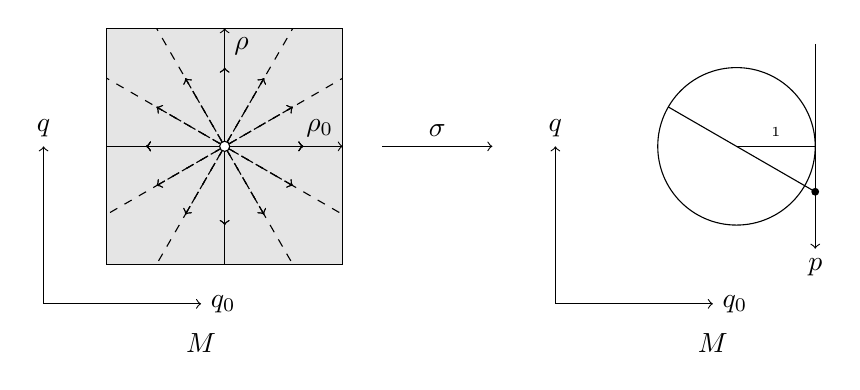
\begin{tikzpicture}
    \draw[->] (0, 0) -- (2, 0) node[anchor=west] {$q_0$};
    \draw[->] (0, 0) -- (0, 2) node[anchor=south] {$q$};
    
    \node (m) at (2.3, 2) {};
    
    \filldraw[draw=black, fill=gray!20] (m) ++(-1.5, -1.5) -- ++(0, 3) -- ++(3, 0) -- ++(0,-3) -- cycle;
    \draw[->] (m) ++(-1.5, 0) -- ++(3, 0) node[anchor=south east] {$\rho_0$};
    \draw[->] (m) ++(0, -1.5) -- ++(0, 3) node[anchor=north west] {$\rho$};
        
    \begin{scope}
        \clip (m) ++(-1.5,-1.5) rectangle ++(3, 3);
        \foreach \i in {0,30,...,180}{
            \draw[<->, dashed] (m) ++({-cos(\i)}, {-sin(\i)}) -- ++({2*cos(\i)}, {2*sin(\i)});
        }
        \foreach \i in {0,30,...,180}{
            \draw[<->, dashed] (m) ++({-cos(\i)}, {-sin(\i)}) -- ++({2*cos(\i)}, {2*sin(\i)});
        }
        \foreach \i in {0,30,...,180}{
            \draw[dashed] (m) ++({-4*cos(\i)}, {-4*sin(\i)}) -- ++({8*cos(\i)}, {8*sin(\i)});
        }
    \end{scope}
    
    \node[circle,draw=black,fill=white,inner sep=1.3pt] at (m) {};
    
    \draw[->] (6.5, 0) -- (8.5, 0) node[anchor=west] {$q_0$};
    \draw[->] (6.5, 0) -- (6.5, 2) node[anchor=south] {$q$};
    
    \node[fill=none] (m2) at (8.8, 2) {};
    
    \draw (m2) circle (1);
    \draw[->] (m2) ++(1, 1.3) -- ++(0, -2.6) node[anchor=north] {$p$} ;
    \draw (m2.center) ++(-0.866, 0.5) -- (9.8, 1.423) node[circle,fill=black, inner sep = 1pt] {};
    \draw (m2.center) -- ++(1, 0) node[pos=0.5,anchor=south] {\tiny{1}};
    %\draw[->] (m) ++(-1.5, 0) -- ++(3, 0) node[anchor=west] {$\rho_0$};
    %\draw[->] (m) ++(0, -1.5) -- ++(0, 3) node[anchor=south] {$\rho$};
    
    \draw[->] (4.3, 2) -- (5.7, 2) node[pos=0.5,anchor=south] {$\sigma$};
     
    \node at (2, -0.5) {$\ctzbundle{M}$};
    \node at (8.5, -0.5) {$\pctbundle{M}$};
\end{tikzpicture}

    \caption{Illustration of the principal $\mgroup$-bundle $\bundle{\ctzbundle{M}}{\pi}{\pctbundle{M}}$. $x$ is a point in the extended configuration space $Q_e$, where we attach fibers $\ctzspace{x}{Q_e}$ and $\pctspace{x}{Q_e}$. The orbits of the group action $\raction{\mgroup}$ on $\ctzbundle{Q_e}$ are identified by $\sigma$ and mapped to the orbit space $\pctbundle{M}$. }
    \label{fig:principal_bundle}
\end{figure}

The space of all orbits is a circle with antipodal points identified, which also has the topology of a circle: this is the space $\mathbb{P}\real$, and it is the fiber $\pctspace{x}{Q_e}$ of $\pctbundle{Q_e}$ at the point $x$. The projection map that takes a point in $\pctbundle{x}{Q_e}$ to its associated orbit in the orbit space is $\sigma$. 

In \cref{fig:principal_bundle}, the coordinate chart used for $\pctbundle{Q_e}$ is indicated as well: $p = -\rho/\rho_0$, which is as the negative of the slope of that line. This coordinate chart covers almost the entire fiber, apart from one `point' (i.e. orbit): the north and south pole of the circle on the right.

From the perspective of $\pctbundle{Q_e}$, $\rho_0$ and $\rho$ can also be seen as \emph{homogeneous coordinates} for this space.

\paragraph{Principal bundles in system theory}
To illustrate the concept of principal bundles and their relevance, we give an instructive example of principal bundles in control theory. For more information, the reader is referred to \citet{Hermann1984}. 

LTI systems can be represented both as a collection of state-space matrices, or in the frequency domain using a transfer matrix. The state-space representation is typically given in the specified by a collection four matrices: $A, B, C, D$. For an LTI system with $n$ states, $m$ inputs and $o$ outputs, we have:
$$ A \in \real^{n \times n} \quad B \in \real^{n \times m} \quad C \in \real^{o \times n} \quad D \in \real^{o \times m}. $$
Hence, the `manifold of LTI systems' given these dimensions is diffeomorphic to \cite{Verhaegen2007} $$\real^{\ell}, \quad \ell = n^2 + nm + on + om.$$  
This is the total space of the principal bundle.

A state space representation of a transfer matrix is not unique: any similarity transform of the state space yields different state space matrices that correspond to the same transfer matrix. Hence, the \emph{structure group} is in this case the general linear group of of dmension $n$, $\glgroup{n}{\real}$, which contains all the similarity transforms. The group action $\raction{\glgroup{n}{\real}} $ is defined as follows:
$$  (A, B, C, D) \raction{T} = (T A T^{-1}, TB, CT^{-1}, D). $$

The orbit space $\real^\ell/\glgroup{n}{\real}$ can be identified with the space of transfer matrices. The projection map that takes the state space represention to a transfer matrix is given by
$$ \sigma(A, B, C, D) = C(s I - A )^{-1} B + D, $$
which is invariant with respect to group action.

The topology of the orbit space, and therefore of the space of transfer matrices, is highly nontrivial. This makes the process of system identification very challenging, for there are usually no easy coordinate charts of this space \cite{Verhaegen2007,Hermann1984}.

\subsubsection{Homogeneous Hamiltonian systems}
In this section, we will lift the contact Hamiltonian system defined in \cref{ssec:contact_dissipation} to the symplectified manifold, resulting in a symplectic Hamiltonian system with an \emph{Liouville structure} additional structure.

\paragraph{Liouville structures} The symplectified space $\ctzbundle{Q_e}$ has a symplectic structure because the cotangent bundle (with zero section removed) is canonically equipped with one. Moreover, the group action that makes it into a principal bundle provides an additional structure: a \emph{symplectic Liouville structure}, which requires that the symplectic 2-form is \emph{homogeneous of degree 1} with respect to the group action $\raction{\mgroup}$. That is,
$$ (\raction{\lambda})^* \omega_e = \lambda\,\omega_e, \qquad \lambda \in \mgroup, $$
which is indeed the case for $\omega_e$ as defined in \cref{eq:symplectic_form_extended} \cite{Libermann1987}. Because the group action $\raction{\mgroup}$ is free, the symplectic Liouville structure is said to be \emph{fibered} \cite{Libermann1987}.

It can be shown that there is again an mapping between the smooth functions on the manifold with Liouville structure and vector fields that preserve this structure\footnote
{For a vector field $X$ to preserve the Liouville structure means (i) that it preserves $\omega_e$, i.e. $\lied{X}{\omega_e} = 0$, and (ii) that it is invariant under the group action: $ (\raction{\lambda})_* X = X$ ($\lambda \in \mgroup)$. }, along the same line as for the symplectic manifolds in \cref{sec:symplectic} and the contact manifolds earlier in this section.

The smooth functions in this case are not completely arbitrary, since they must also comply with the Liouville structure. More precisely, they must be \emph{homogeneous} of degree 1 with respect to the group action $\raction{\mgroup}$. For a function $\mathscr{H}$ on $\ctzbundle{Q_e}$ to be homogeneous means it must satisfy the following condition
$$ (\raction \lambda )^* \mathscr{H} = \lambda \mathscr{H}. $$
In the coordinates defined above, this is equivalent to:
$$ \mathscr{H}(q_0, q, \lambda \rho_0, \lambda \rho) = \lambda\mathscr{H}(q_0, q, \rho_0, \rho) \qquad \lambda \in \mgroup,$$
which is to say that $\mathscr{H}$ \emph{commutes} with the group action.

Thus, we have an isomorphism between the vector fields preserving the Liouville structure and the homogeneous functions on the manifold. 
This manifold is symplectic, so isomorphism is defined in terms of the symplectic form $\omega_e$ like so (and in identical fashion to \cref{eq:symplectic_isomorphism}),
$$ \fromDual{\omega_e}(\dd{\mathscr{H}}) = X_\mathscr{H}. $$

This gives rise to the notion of \emph{homogeneous Hamiltonian systems}, consisting of a manifold with fibered symplectic Liouville structure and a homogeneous Hamiltonian function $\mathscr{H}$.

\paragraph{Equations of motion} The contact Hamiltonian system for the damped harmonic oscillator, as defined by \cref{eq:dho_contact_hamiltonian_e}, can now be lifted to a homogeneous Hamiltonian system on the symplectified space. The relation between the contact Hamiltonian and the corresponding homogeneous Hamiltonian is defined as \cite{VanderSchaft2021a,Libermann1987,Arnold1989}
$$ K_e(q_0, q, p) = \mathscr{H}(q_0, q, -1, \rho), $$
or equivalently
\begin{equation}
    K_e\qty(q_0, q, -\frac{\rho}{\rho_0}) = \mathscr{H}(q_0, q, \rho_0, \rho). 
    \label{eq:H_contact_homo}
\end{equation}

Based on \cref{eq:dho_contact_hamiltonian_e}, we obtain the following expression for the homogeneous Hamiltonian:
\begin{equation}
    \mathscr{H}(q_0, q, \rho_0, \rho) = -\rho_0\,\qty[\frac{1}{2m}\qty(-\frac{\rho}{\rho_0})^2 + \frac{1}{2}kq^2 + \gamma q_0]. 
    \label{eq:H_dho_homo}
\end{equation}

The Hamiltonian vector field is easily obtained, for we can use the mapping $\fromDual{\omega_e}$. As already mentioned this is a major advantage of performing calculations in the symplectified space. We have
$$ X_\mathscr{H} = \fromDual{\omega_e}(\dd{\mathscr{H}}),$$ 
with
$$ \dd{\mathscr{H}} = \pdv{\mathscr{H}}{q_0}\dd{q_0} 
                      + \pdv{\mathscr{H}}{q}\dd{q}
                      + \pdv{\mathscr{H}}{\rho_0}\dd{\rho_0}
                      + \pdv{\mathscr{H}}{\rho}\dd{\rho}.
$$

It is instructive to first specify the partial derivatives of $\mathscr{H}$ in terms of $K_e$, so as to compare the generic equations of motion obtained from $\mathscr{H}$ to those obtained from $K_e$ (cf. \cref{eq:ham_vf_e}). Using \cref{eq:H_contact_homo}, the partial derivatives can be expressed in terms of the contact Hamiltonian $K_e$:
\begin{equation}
    \begin{split}
        \pdv{\mathscr{H}}{q} &= -\rho_0 \pdv{K_e}{q}, \\
        \pdv{\mathscr{H}}{q_0} &= -\rho_0 \pdv{K_e}{q_0}, \\
        \pdv{\mathscr{H}}{\rho} &= -\rho_0 \pdv{K_e}{p}\pdv{p}{\rho} = \pdv{K_e}{p}, \\
        \pdv{\mathscr{H}}{\rho_0} &= -H - \rho_0 \pdv{K_e}{p}\pdv{p}{\rho_0} = -K_e - \pdv{H}{p}\frac{\rho}{\rho_0} = \pdv{H}{p}p - K_e.\\
    \end{split}
    %\label{eq:partial_relation}
\end{equation}
The homogeneous Hamiltonian vector field is then
\begin{equation}
    X_\mathscr{H} = \qty(\pdv{K_e}{p}p - K_e)\pdv{}{q_0}
                    + \pdv{K_e}{p}\pdv{}{q}
                    + \rho_0\pdv{K_e}{q_0}\pdv{}{\rho_0}
                    + \rho_0\pdv{K_e}{q}\pdv{}{\rho}.
    \label{eq:hom_ham_vf}
\end{equation}
%\begin{equation}
%    \begin{split}
%        &\dot{q}_0      = \pdv{H}{p}p - H, \\
%        &\dot{q}        = \pdv{H}{p}, \\
%        &\dot{\rho}_0   = \rho_0\pdv{H}{q_0}, \\
%        &\dot{\rho}     = \rho_0 \pdv{H}{q}.
%    \end{split}
%\end{equation}
The equations of motion $q_0$ and $q$ remain identical to those obtained earlier; this is to be expected since otherwise the dynamics would not correspond. 

For $\rho_0$, we have
$$ \dot{\rho}_0 = \rho_0 \pdv{K_e}{q_0} = \rho_0 \pdv{K_e}{q_0}  = \gamma\rho_0 \quad \Rightarrow \quad \rho_0 = \ec^{\gamma t} + C, $$ 
where $C$ is an integration constant which we can choose to be 0, so $\rho_0(t) = \ec^{\gamma t}$.

In addition, $\dot{\rho} = \rho_0 kq = \ec^{\gamma t} kq$. Since $p = -\rho/\rho_0$, the dynamics of $p$ can be obtained from  $\dot{\rho}_0$ and $\dot{\rho}$ using the product rule:
\begin{equation} 
    \dot{p} = -\frac{\dot{\rho}}{\rho_0} + \frac{\rho}{\rho_0}\frac{\dot{\rho}_0}{\rho_0} = -kq - \gamma p,
    \label{eq:pdot}
\end{equation}
which is equivalent to the expression obtained in \cref{ssec:contact_dissipation}.

Observe that these equations of motion are invariant under the earlier defined group action $\raction{\mgroup}$, which means that the vector field indeed preserves the Liouville structure. The other condition is that it preserves $\omega_e$, but this is satisfied rather trivially as a result of the mapping $\fromDual{\omega_e}$.
%The Hamiltonian vector field then becomes
%\begin{equation}
%    X_{\mathscr{H}} = -\frac{1}{m}\frac{\rho}{\rho_0}\pdv{}{q}\: + \: \qty[\frac{1}{2m}\qty(\frac{\rho}{\rho_0})^2 - \frac{1}{2}kq^2 - \gamma q_0]\pdv{}{q_0}\: + \: \rho_0 kq \pdv{}{\rho}\: + \: \gamma \rho_0 \pdv{}{\rho_0}.
%    \label{eq:homo_vf}
%\end{equation}

\paragraph{Liouville submanifolds} In \cref{ssec:contact_dissipation} we devoted considerable attention to the fact that the contact Hamiltonian should numerically be equal to zero for the equations of motion to represent a physical trajectory. This is equivalent to stating that the trajectories lie in Legendre submanifolds.

As pointed out by \citet{VanderSchaft2021a} and \citet{Libermann1987}, because of the equivalence between contact and Liouville structures, the notion of Legendre submanifolds can be lifted to the symplectified space as well. Indeed, from \cref{eq:liouville_form_extended} we can observe that if $\alpha_e$ pulls back to zero on the trajectories in the contact manifold, so should $\theta_e$ on the lifted trajectories, for they only differ by multiplication with $\rho_0$. These are called \emph{Liouville submanifolds}, and are a special subclass of Lagrangian submanifolds\footnote{Lagrangian submanifolds satisfy the weaker condition that the symplectic 2-form $\omega_e$ vanishes when restricted to them. This is also the case when $\theta_e$ vanishes, but the converse is not necessarily true.}

Using \cref{eq:hom_ham_vf}, we find that 
$$ \intpr{X_\mathscr{H}}{\theta_e} = -K_e, $$
which means that the contact Hamiltonian (i.e. the total energy in the system)
must be equal to zero for the lifted trajectories to lie in a Liouville submanifold.

For yet another perspective regarding this point, we can make use of the symplectic nature of the homogeneous Hamiltonian. Indeed, no matter what the value of $K_e$, the homogeneous Hamiltonian $\mathscr{H}$ \emph{must} be constant over time, because it does explicitly depend on it. Since the dynamics are symplectic, we can simply use Poisson brackets support this fact:
$$ \dot{\mathscr{H}} = \poisson{\mathscr{H}}{\mathscr{H}} + \pdv{\mathscr{H}}{t} = 0.$$

Hence, we can set the Hamiltonian equal to a constant, say $\mathscr{H}(t) = \mathscr{H}_0$. But, we also know from $\mathscr{H} = \rho_0 K_e = \ec^{\gamma t} K_e$. Hence, it is now very easy to see that $K_e$ eithe  decays exponentially (if $\gamma > 0$), for it then cancels exactly the exponential growth of $\rho_0$, or it equal to zero. This is equivalent to \cref{eq:contact_ham_growth}. On Liouville submanifolds, both the homogeneous Hamiltonian and the contact Hamiltonian vanish, which amounts to the particular choice that $\mathscr{H}_0 = 0$.

If we assume that the dynamics take place on a Liouville submanifold, the Hamiltonian vector field becomes
$$ X_\mathscr{H}\vert_{\mathscr{H}_0 = 0} =  -\frac{1}{m}\frac{\rho}{\rho_0}\pdv{}{q}\: + \: \pdv{}{q_0}\: + \: \rho_0 kq \pdv{}{\rho}\: + \: \gamma \rho_0 \pdv{}{\rho_0}. $$
If this vector field is be projected to $\pctbundle{Q_e}$ using the pushforward of the projection map $\sigma$, we obtain \cref{eq:ham_vf_e_liouville}.\footnote{This is the `differential geometric' way of deriving the equation for $\dot{p}$ as we did above.}

\subsubsection{Relation with the Caldirola-Kanai Hamiltonian}
In this section, we show that the homogeneous Hamiltonian is equivalent to a well-known existing model for the damped harmonic oscillator, the Caldirola-Kanai Hamiltonian (and Lagrangian).

The Caldirola-Kanai Hamiltonian, commonly attributed to \citet{Caldirola1941} and \citet{Kanai1948}, is a method to describe the linearly damped harmonic oscillator using a Lagrangian or Hamiltonian function that explicitly depend on time. It was originally motivated for the purposes of quantum mechanics.

We depart from the Lagrangian function for it depends directly on physical coordinates $q$ and $\dot{q}$, as opposed to the Hamiltonian. The Caldirola-Kanai Lagrangian is
\begin{equation}
    \Lck(q, \dot{q}, t) = \ec^{\gamma t}\qty(\frac{1}{2}m\dot{q}^2 - \frac{1}{2}kq^2).
    \label{eq:lag_CK}
\end{equation}
The correct equations of motion are readily derived through the Euler-Lagrange equations:
\begin{equation}
    \begin{split}
        \dv{}{t}\qty(\pdv{\Lck}{\dot{q}}) - \pdv{\Lck}{q} &= 0, \\
        \dv{}{t}\qty(\ec^{\gamma t } m \dot{q}) + \ec^{\gamma t} kq &= 0, \\
        \ec^{\gamma t } \qty(m\ddot{q} + m\gamma\dot{q} + kq)  &= 0, \\
        m\ddot{q} + m\gamma\dot{q} + kq &= 0. \\
    \end{split}
\end{equation}

The Caldirola-Kanai Hamiltonian is obtained from the Lagrangian by means of a Legendre transform. The Legendre transfrom is effected with respect to the \emph{canonical momentum}
$$ \rho = \pdv{\Lck}{\dot{q}} = \ec^{\gamma t} m \dot{q}, $$
which is manifestly different from the kinematic momentum $p = m\dot{q} = \rho \ec^{-\gamma t}$.

The Hamiltonian is then equal to
$$ \Hck = \rho\dot{q} - \Lck =  \frac{\Pcan^2}{2m}\ec^{-\gamma t} + \frac{1}{2}kq^2\ec^{\gamma t}. $$
Because the Hamiltonian is explicitly time-dependent, the associated Hamiltonian vector field will be time-dependent as well\footnote
{A \emph{time-dependent vector field} on a manifold $N$ is a mapping $X: N\times\real \to \tbundle{N}$ such that for each $t \in \real$, the restriction $X_t$ of $X$ to $N \times \{t\}$ is a vector field on $N$. \cite{Libermann1987} An additional construction of importance, called the \emph{suspension} of the vector field, is a mapping $$ \tilde{X}: \real \times N \to \tbundle{(\real \times N)} \quad (t, n) \mapsto ((t, 1), (n, X(t, n))),$$ that is to say, the suspension lifts the vector field to the extended space that also includes $t$ and assigns the time coordinate with a trivial velocity of 1 \cite{Abraham1978}.}.

The construction of the vector field associated with a time-dependent Hamiltonian follows the same construction rules as a normal Hamiltonian using the isomorphism given by $\fromDual{\omega}$, but `frozen' at each instant of $t$. The Hamiltonian vector field on $\ctbundle{Q}$ is
$$ X_{\Hck} = -\ec^{\gamma t}kq\pdv{}{\Pcan} + \ec^{-\gamma t}\frac{\Pcan}{m}\pdv{}{q}.$$

The suspension of this vector field on $\ctbundle{Q}\times \real$ is
$$ \tilde{X}_{\Hck} = -\ec^{\gamma t}kq\pdv{}{\Pcan} + \ec^{-\gamma t}\frac{\Pcan}{m}\pdv{}{q} + \pdv{}{t}.$$
The suspension is important because it allows us to perform the time-dependent transformation from the canonical momentum $\rho$ to the kinematic momentum $p$:
$\phi: (q, \Pcan, t) \mapsto (q, \ec^{\gamma t}p, t).$
The transformed vector field in terms of the physical coordinates $p, q, t$ is
$$ \phi_*(\tilde{X}_{\Hck}) = \qty(-kq - \gamma p)\pdv{}{p} + \frac{p}{m}\pdv{}{q} + \pdv{}{t}.$$
The extra term in $p$ arises as a consequence of the fact that the mapping from $\rho$ to $p$ depends also on $t$. 

The similarity between the derivation of the equations of motion --- in particular, the crucial role of the product rule --- and the one given by \cref{eq:pdot} is striking. Indeed, if we substitute into the Caldirola-Kanai Hamiltonian $-\rho_0 = \ec^{\gamma t}$, we obtain
$$ \Hck = -\frac{\rho^2}{2m\rho_0} - \rho_0 \frac{1}{2}kq^2 = -\rho_0 \qty (\frac{1}{2m}\qty(\frac{\rho}{\rho_0})^2 + \frac{1}{2}kq^2), $$
which is precisely equal to the homogeneous Hamiltonian given in \cref{eq:H_dho_homo} excluding the term in $q_0$. The depence on $q_0$ is not required, since it is replaced by an explicit dependence on time that would otherwise generate the exponential factor $\ec^{\gamma t}$. 

Many interpretations have already been given for the particular form of $\Hck$; for example through time-dependent canonical transformations, or by a rescaling of time itself (see i.a. \citet{Tokieda2021}, \citet{Caldirola1941} and \citet{Bravetti2017}). Here we can see that the Caldirola-Kanai can be regarded as  directly equivalent to the homogeneous Hamiltonian system, where the dynamics of the additional coordinates $\rho_0$ and $q_0$ are replaced by their explicit solution in time. Additionally, the role of the `mysterious' canonical momentum $\rho$ is explained as being a coordinate of the symplectified space, or homogeneous coordinate for the underlying contact space\footnote{This has caused considerable confusion in literature, as stated by \citet{Schuch1997}.}.

\subsection{The harmonic oscillator with serial damping}
In this section, we extend the method outlined in \cref{ssec:contact_dissipation} to a harmonic oscillator with two dampers: one in series and one in parallel. This system will play an important role in \cref{chap:quaternion}.
\begin{figure}[ht!]
    \centering
    \begin{tikzpicture}[every node/.style={outer sep=0pt,thick}]
    % Spring style
    \tikzstyle{spring} = [thick, 
                          decorate,
                          decoration={zigzag,pre length=0.2cm,post length=0.2cm,segment length=6}]

    % Damper style
    \tikzstyle{damper}= [thick, 
                         decoration={markings,  
                         mark connection node=dmp,
                         mark=at position 0.5 with 
                         {
                           \node (dmp) [thick,inner sep=0pt,transform shape,rotate=-90,minimum width=15pt,minimum height=3pt,draw=none] {};
                           \draw [thick] ($(dmp.north east)+(2pt,0)$) -- (dmp.south east) -- (dmp.south west) -- ($(dmp.north west)+(2pt,0)$);
                           \draw [thick] ($(dmp.north)+(0,-5pt)$) -- ($(dmp.north)+(0,5pt)$);
                         }
                        }, decorate]
                        
    \tikzstyle{ground} = [fill, 
                          pattern = north east lines, 
                          draw = none,
                          minimum width = 0.75cm,
                          minimum height = 0.3cm]

    \node (M) [draw,minimum width=1cm, minimum height=1.5cm] {$m$};

    \node (ground) [ground,anchor=north,yshift=-0.25cm,minimum width=1.5cm] at (M.south) {};
    \draw (ground.north east) -- (ground.north west);
    \draw [thick] (M.south west) ++ (0.2cm,-0.125cm) circle (0.125cm)  (M.south east) ++ (-0.2cm,-0.125cm) circle (0.125cm);

    \node (wall) [ground, rotate=-90, minimum width=2.5cm,yshift=-3cm] {};
    \node [xshift=-1.2cm, circle, fill=black, inner sep = 1pt] (p1) at ($(M.north west)!(wall.160)!(M.south west)$) {};
    %\node [yshift=0.3cm] at (p1) {$q_1$};
    \draw (wall.north east) -- (wall.north west);
    %\node[anchor=south] at (M.north) {$q_2$};

    \node[above=1.5cm of wall, outer sep = 0mm, inner sep=0mm] (p3) {};
    \node[above=2.3cm of wall, outer sep = 0mm, inner sep=0mm] (p4) {};


    \path (p3) -| node[outer sep = 0mm, inner sep=0mm] (p5) {} (p1);
    \path (p4) -| node[outer sep = 0mm, inner sep=0mm] (p6) {} (M);

    \draw[|->] (p3) -- (p5) node[anchor=south,pos=0.5] {$q$};
    \draw[|->] (p4) -- (p6) node[anchor=south,pos=0.5] {$q_1$};

    \draw (p5) ++(0, 0.2) -- ++(0,-1.2);
    \draw (p6) ++(0, 0.2) -- ++(0,-1.7);

    %\node (coord1) [yshift=1.5cm, minimum width=0.3cm] at (wall) {};
    %\draw[->] (coord1) -- ++(1cm, 0);

    \draw [spring] (wall.160) -- (p1) node[pos=0.5,anchor=south, outer sep=4pt] {$k$};
    \draw [damper] (wall.20) -- ($(M.north west)!(wall.20)!(M.south west)$) node[pos=0.5, anchor=north, outer sep=8pt] {$b_p$};
    \draw[damper] (p1) -- ($(M.north west)!(wall.160)!(M.south west)$) node[pos=0.5, anchor=south, outer sep=8pt] {$b_s$};


    \node[bgelement, label=west:$q$] (J0) at (3.5, 0.5) {0};

    \node[bgelement, label=east:$p$] (J1) at (5, 0.5) {1};

    \node[bgelement, label=north:$k$] (C) at (3.5, 2) {C};
    \node[bgelement, label=south:$b_s$] (Rs) at (3.5, -1) {R};

    \node[bgelement, label=north:$m$]  (I) at (5, 2) {I};
    \node[bgelement, label=south:$b_p$]  (Rp) at (5, -1) {R};

    % test
    \draw[bonds] 
        (J1) edge[e_out] (I)
        (J1) edge[f_out] (Rp)

        (J0) edge[f_out] (C)
        (J0) edge[e_out] (Rs)
        (J0) edge[e_out] (J1);

\end{tikzpicture}

    \caption{Schematic of the harmonic oscillator with two dampers: one in series and one in parallel. The corresponding bond graph representation is shown on the right.}
    \label{fig:double_damped_osc}
\end{figure}

The harmonic oscillator with two dampers is shown in \cref{fig:double_damped_osc}, together with the corresponding bond graph representation. Comparing this to \cref{fig:dho}, there is another 0-junction present in the system that compares flows (velocities) rather than efforts (forces). The equations of motion can be readily derived:
\begin{equation}
    \begin{split}
        m\ddot{q}_1 &= -kq - b_p \dot{q}_1 \\
        kq &= b_s(\dot{q}_1 - \dot{q}) \\
    \end{split}
    \label{eq:serial_eom_raw}
\end{equation}
Due to the presence of the serial damper, the situation is somewhat curious, since there are two positions in the system; one measuring the spring deflection $q$ and the position of the mass $q_1$. The subscript `1' refers to the fact that $q_1$ is the position measured at the 1-junction in the bond graph shown in \cref{fig:dho}. However, the node connecting the serial damper and the spring has no mass, and therefore no second-order dynamics: as such, the overall order of the system is two. 

In accordance with the economic analogy, we will say that position is stored in the spring, but momentum is stored in a mass.
Hence, we let $p = m\dot{q}_1$ --- but $\dot{q} \neq p/m$ in general. That is to say, the spring is naturally associated with a position coordinate, while the mass has a momentum, though its position does not partake in the dynamics directly.

Using the damping coefficients defined in \cref{tab:ddho_params}, the equations om motion become:
\begin{equation}
    \begin{split}
        \dot{q} &= -\gamma_s q + p/m  \\
        \dot{p} &= -\gamma_p p - kq.
    \end{split}
    \label{eq:serial_eom_pq}
\end{equation}

%In addition to $q_1$ being the position measured at the 1-juncton, we can also measure the momentum at the 0-junction, this momentum is $p_0 \coloneq m\dot{q}$. Again, the subscript `0` refers to the fact that is momentum is based on the 0-junction, along the same line as the position coordinate $q_1$. Hence, we have four coordinates, two of which  ($p$ and $q$), are natural because they are measured at the component of the where they are effectively stored. In addition there are $p_0$ and $q_1$, which are somewhat artificial definitions.
\begin{table}[ht!]
    \caption{Substition parameters for the harmonic oscillator with serial and parallel damping, shown in \cref{fig:double_damped_osc}.}
    \label{tab:ddho_params}
    \centering
    \begin{tabular}{llll}
        \toprule
        \textbf{Name} & \textbf{Symbol} & \textbf{Value} & \textbf{Units} \\
        \midrule
            Serial damping coefficient & $\gamma_s$ & $k/b_s$ & \si{\per \second} \\
            Parallel damping coefficient & $\gamma_p$ & $b_p/m$ & \si{\per \second} \\
            Natural frequency & $\Omega_n$ & $\sqrt{k/m}$ & \si{\per \second} \\
            Damped frequency & $\Omega_d$ &  & \si{\per \second} \\
        \bottomrule
    \end{tabular}
\end{table}

\paragraph{Contact Hamiltonian system} In order to establish the contact structure for the harmonic oscillator with two dampers, we must find the expression for the work done by the system on the dampers. We will do so using the structure of the bond graph shwon in \cref{fig:double_damped_osc}. 

Bonds carry two signals: an effort and a flow. Both can be assigned a `direction'; they are always opposite. The direction indicates whether either the effort or flow should be regarded as the `input' of the model. For example, \emph{traditionally} (though this is a matter of convention), an I-element takes efforts as an input, and returns a flow. That is to say, one applies a force to a mass, with a change in velocity as a result. Conversely, when a spring is stretched along a certain distance to return a force proportional to it; it takes a flow and returns an effort \cite{Borutzky2010}. In a bond graph, this is indicated by a causality stroke, which is placed at the side of the bond that determines the flow.

If a causality convention is chosen, all the I- and C-elements in the bond graph should conform to this convention\footnote{Not doing so leads to a differential algebraic system (DAE).}. This is \emph{not} the case for R-elements; they are \emph{indifferent to causality}. The reason for this is that there is no integral/derivative present in the mathematical description of their dynamic behavior: they relate an effort and flow, which are both time derivatives. So, depending on the system architecture, a particular R-element may receive an effort and return a flow, or vice versa \cite{Borutzky2010}.

This can be observed from \cref{fig:double_damped_osc}: the serial damper (on the 0-junction) receives an effort and returns a flow, while the parallel damper receives a flow and returns an effort (1-junction). This distinction is reflected in the work form associated to the damper. For the parallel damper, we have
$$ \beta_p = \underbrace{\gamma_p p}_\text{\textsc{effort}} \; \underbrace{\dd{q}.}_\text{\textsc{flow}} $$
The variable that is `varied' externally is the flow, hence $\dd{q}$ 

For the serial damper, we have the opposite situation. Here, the effort is varied externally, which is equal to $-\dd{p}$. The flow is equal to $\dot{q}_1 - \dot{q} = kq/b_s = \gamma_s q$ (using \cref{eq:serial_eom_raw}). Hence, we have
$$ \beta_s = \underbrace{\gamma_s q}_\text{\textsc{flow}} \; \underbrace{-\dd{p}.}_\text{\textsc{effort}}$$

Combining these work forms, we find the contact form for the system with two dampers:
\begin{equation}
    \alpha = \dd{U} - \gamma_p p\dd{q} + \gamma_s q \dd{p}.
    \label{eq:serial_dho_contact_form}
\end{equation}
The exterior derivative of the contact form $\alpha$ is then equal to
$$ \dd{\alpha} = (\gamma_s + \gamma_p) \wedgep{\dd{q}}{\dd{p}}, $$
and the Reeb vector field is simply
$$ R_\alpha = \pdv{}{U}. $$

Now to find the Hamiltonian and the system dynamics. In the following, we will only consider the horizontal component of the Hamiltonian vector field, for the various reasons pointed out in \cref{ssec:contact_dissipation,ssec:symplectification}. The horizontal component is given by (cf. \cref{eq:horizontal_vf}):
\begin{equation}
    \begin{split}
        X^\text{hor}_K &= \fromDual{\dd{\alpha}}\qty(\dd{K} - (\intpr{R_\alpha}{\dd{K}})\alpha) \\
                       &= \fromDual{\dd{\alpha}}\qty(\qty(\pdv{K}{q} + \gamma_p p \pdv{K}{U})\dd{q} + \qty(\pdv{K}{p} - \gamma_s q \pdv{K}{U})\dd{p}).
    \end{split}
\end{equation}

The mapping $\fromDual{\dd{\alpha}}$ acts on the basis 1-forms as follows:
$$ 
    \fromDual{\dd{\alpha}}(\dd{p}) = \frac{1}{\gamma_s + \gamma_p}\qty(\pdv{}{q} + \gamma_p p\pdv{}{U}) \qquad
    \fromDual{\dd{\alpha}}(\dd{q}) = \frac{1}{\gamma_s + \gamma_p}\qty(-\pdv{}{p} + \gamma_s q\pdv{}{U}).
$$
The extra terms in $\pdv{}{U}$ appear again to ensure that the vector field be horizontal.

Using the same reasoning applied in \cref{ssec:contact_dissipation}, we can observe that the contact Hamiltonian must be proportional to the sum of the mechanical and internal energy of the system. In addition, we wish to cancel the factor $(\gamma_s + \gamma_p)$ present in the mapping $\fromDual{\dd{\alpha}}$ by multiplying the contact Hamiltonian with the same factor. Hence we, have
$$ K = (\gamma_s + \gamma_p)\qty(\frac{p^2}{2m} + \frac{1}{2}kq^2 + U). $$

Assuming again that $K = 0$, the contact Hamiltonian vector field is then:
$$ X_K = X_K^\text{hor} = \qty(\frac{p}{m} - \gamma_s q)\pdv{}{q} + \qty(-kq -\gamma_p p)\pdv{}{p} + \qty(\gamma_p\frac{p^2}{m} + \gamma_s kq^2 )\pdv{}{U}, $$
since the cross terms in $\pdv{}{U}$ cancel out. Next to the familiar dissipated power for the parallel damper, we also have the dissipated power of the serial damper
$$ \gamma_s kq^2 = \underbrace{\gamma_s q}_\text{\textsc{flow}} \: \times \underbrace{kq}_\text{\textsc{effort}}, $$ 
in the dynamics of $U$. Hence, this vector field yields the correct dynamics for $p$ and $q$ as given by \cref{eq:serial_eom_pq}, in addition to the internal energy $U$.

%In order to apply the procedure outlined in \cref{ssec:contact_dissipation}, we first perform a coordinate transform to get rid of one of the two junctions in the system. This can be done by expressing the dynamics either in terms of $q$ and $p_0$, or alternatively, in terms of $p$ and $q_1$. This is equivalent to moving all the bond graph elements to one of the two junctions. 
%
%Using the equations of motion \cref{eq:serial_eom_raw} and the definition of $p_0$ to find that
%$$ p_0 = p -m\gamma_s q, $$
%which is in reality not so much a momentum as the impulse that acts on the connection point between the serial damper and the spring. Hence, we have a linear coordinate transformation
%$$ \phi:\quad \mqty(q \\ p_0) = \mqty(1 & 0 \\ -m\gamma_s & 1)\mqty(q \\ p). $$
%Observe that this is a symplectic transformation\footnote
%{
%    A symplectic matrix $T$ is a matrix that satisfies the relation \cite{Abraham1978}
%    $$ T^\top J T = J \qquad \text{with}\quad J = \mqty(0 & I \\ -I & 0 ).$$
%
%}.
%The vector field corresponding to the equations of motion \cref{eq:serial_eom_pq} is
%$$ X = \qty(-\gamma_s q + \frac{p}{m})\pdv{}{q} + \qty(-\gamma_p p - kq)\pdv{}{p}. $$
%The unit vectors transform under $\phi_*$ as follows,
%$$ \phi_* \pdv{}{q} = \pdv{}{q} - \gamma_s \pdv{}{p_0} \qquad \phi_* \pdv{}{p} = \pdv{}{p_0}. $$
%Hence, the transformed vector field is
%$$ \phi_* X = \frac{p_0}{m}\pdv{}{q} + \big[-(\gamma_p + \gamma_s)p_0 - (m \gamma_s \gamma_p + kq)q\big]\pdv{}{p_0}. $$
%The transformed vector field is \emph{second-order} (when expressed in the velocities) in contrast to the original one. Roughly speaking, in a second order vector field the rate of change of the position coordinates is actually equal to the velocity coordinate. For a more rigorous definition, the reader is referred to \cref{app:symplectic_geometry}. 
%
%The transformed vector field is of the same form as the one used in \cref{ssec:contact_dissipation}, but now for adjusted expressions for the damping coefficient 
%$$\gamma \mapsto \gamma_s + \gamma_p,$$ 
%and the spring constant 
%$$k \mapsto k + m\gamma_s\gamma_p.$$ 
%Hence, we can translate this to a contact Hamiltonian system in a completely analogous fashion. The contact 1-form is
%$$ \alpha = \dd{U} - (\gamma_s + \gamma_p)p_0\dd{q}, $$
%and contact Hamiltonian
%$$ K = \frac{p_0^2}{2m} + \frac{1}{2}(m \gamma_s\gamma_p + k)q^2. $$

%The nontrivial relation between momentum and precludes the associated vector field from being second-order, when expressed in terms of the velocities. A second-order vector field implies that the velocities really are the time derivatives of the positions, (cf. \cref{app:symplectic_geometry} for a more formal discussion).



